\documentclass[11pt]{report}
\usepackage[
  dissertation
 ,final
 ,raggedbottom
]{USCthesis}


% Brandon's packages
\usepackage{tikz}
\usepackage{pgfplots}
\pgfplotsset{compat=1.11}
\usepgfplotslibrary{groupplots}
\usetikzlibrary{decorations}
\usetikzlibrary{decorations.markings}
\usepgfplotslibrary{fillbetween}
\pgfplotsset{%
	actfunc/.style = {%
		domain=-5:3,
		samples = 400,
		smooth,
		thick,
		on layer={axis foreground},
	}
}

\usepackage{listings}
%\usepackage{amsmath}
\usepackage{mathtools}
\usepackage{xcolor}

\lstset{ %
	backgroundcolor=\color{white},   % choose the background color
	basicstyle=\footnotesize\ttfamily,        % size of fonts used for the
	%code
	columns=fullflexible,
	breaklines=true,                 % automatic line breaking only at
	%whitespace
	captionpos=b,                    % sets the caption-position to bottom
	tabsize=4,
	commentstyle=\color{mygreen},    % comment style
	escapeinside={\%*}{*)},          % if you want to add LaTeX within your
	%code
	keywordstyle=\color{blue},       % keyword style
	stringstyle=\color{mymauve}\ttfamily,     % string literal style
	frame=single,
	rulesepcolor=\color{red!20!green!20!blue!20},
	% identifierstyle=\color{red},
	language=c++,
	escapechar=!
}

\usepackage{comment}
\usepackage{algorithm2e}
\usepackage{amsthm}
\usepackage{multirow}
\usepackage{makecell}
\usepackage{amsmath}
\usepackage{float}

% Brandon's commands
\newcommand{\declarecommand}[1]{\providecommand{#1}{}\renewcommand{#1}}
\DeclareMathOperator*{\argmin}{argmin}
\DeclareMathOperator*{\argmax}{argmax}
\newcommand*{\argminl}{\argmin\limits}
\newcommand*{\argmaxl}{\argmax\limits}


%\tikzset{\font={\fontsize{8pt}{12}\selectfont}}

% guidelines for manuscript formatting:
%http://graduateschool.usc.edu/wp-content/themes/fictional-university-theme/assets/doc/Manuscript_Formatting_and_Documentation_Styles.pdf

%% our customizations %%%%%%%%%%%%%%%%%%%%%%%%%%%%%%%%%%%%%%%%%%%%%%%%%%
\usepackage[export]{adjustbox} % for frame option in \includegraphics
\usepackage{amssymb}
\usepackage{array}
\usepackage[utf8]{inputenc} % load inputenc before csquotes
\usepackage[english]{babel}
\usepackage[
  backend     = biber,
  doi         = true,
  hyperref    = true,
  maxbibnames = 99,
  sortlocale  = en_US,
  style       = numeric,
]{biblatex}
\usepackage{booktabs}
\usepackage{color, colortbl}
\usepackage{csquotes}
\usepackage{efbox}
\usepackage{enumitem}
\usepackage[shortcuts]{extdash} % use `\-/' to hyphenate words/phrases that have a dash in them
\usepackage[tt=false]{libertine} % libertine's \ttfamily isn't that great
\usepackage[T1]{fontenc} % load fonts before fontenc
\usepackage[symbol]{footmisc}
\usepackage[
  showframe = false,% draw a border around textwidth
  pass      = true, % force 8.5"x11" pagesize
]{geometry}
\usepackage{graphicx}
%\usepackage[notquote]{hanging} % enables negative indents in paragraphs
\usepackage{hyphenat}
\usepackage{ifthen}
\usepackage{lipsum}
\usepackage{multirow}
\usepackage{parnotes}
\usepackage{pdflscape} % rotate some pages in an {landscape} environment
\usepackage{pifont}
\usepackage{ragged2e}
\usepackage{seqsplit}
\usepackage{siunitx}
\usepackage{subcaption}
\usepackage{tabularx}
\usepackage{xcolor}
\usepackage{xspace}
\usepackage{url}

\usepackage[
  breaklinks    = true,
  colorlinks    = true,
  hypertexnames = false,
  pdfpagelabels = false,
  citecolor     = {blue!80!black},
  linkcolor     = {blue!80!black},
  urlcolor      = {blue!80!black},
]{hyperref} % load hyperref as the last package

% pkg: biblatex
\setlength\bibitemsep{0.5\baselineskip}                 % add a line between entries
\AtEveryBibitem{\iffieldundef{doi}{}{\clearfield{url}}} % if DOI, hide URL

\addbibresource{paper.bib}

% pkg: siunitx
% some guidelines https://physics.nist.gov/cuu/Units/checklist.html
\sisetup{
  tight-spacing  = true
  ,detect-family = true
  ,detect-mode   = true
  ,binary-units  = true    % support for MB, GB, etc.
  ,range-units   = single  % "3% to 5%" -> "3 to 5%"
  ,range-phrase  = --      % "3 to 5%"  -> "3--5%"
}

% pkg: babel, hyperref
\addto\extrasenglish{%
  \renewcommand{\chapterautorefname}{Chapter}
  \renewcommand{\sectionautorefname}{Section}
  \renewcommand{\subsectionautorefname}{Section}
  \renewcommand{\subsubsectionautorefname}{Section}
}

% pkg: url
\renewcommand{\UrlFont}{\footnotesize\tt}

% our custom commands
\renewcommand{\ttdefault}{cmtt} % use computer modern for teletype

%%% draft mode / toggle commands %%%
\usepackage{etoolbox}
\newtoggle{draft}
\settoggle{draft}{false} % change toggle for draft or final versions

\iftoggle{draft}{
  % if 'draft' toggle is true
  \overfullrule=10pt                       % highlight overfull hboxes
}{
  % if 'draft' toggle is false
  \PassOptionsToPackage{final}{showlabels} % hide labels on figures, etc
}

% if you're including existing papers into your thesis, it helps to put
% content behind a toggle (or conditional) so you only have to maintain
% and keep consistency on one copy. see "introduction.tex".
\newtoggle{thesis}
\settoggle{thesis}{true}

\usepackage[inline]{showlabels}
\renewcommand{\showlabelfont}{\sffamily \color{blue}}
\renewcommand{\showlabelsetlabel}[1]{\efbox{\showlabelfont #1}}
%%%%%%%%%%%%%%%%%%%%%%%%%%%%%%%%%%%%%%%%%%%%%%%%%%%%%%%%%%%%%%%%%%%%%%%%

%%% front matter %%%%%%%%%%%%%%%%%%%%%%%%%%%%%%%%%%%%%%%%%%%%%%%%%%%%%%%
\begin{document}

% title should be all caps
\title{Differential Verification of Deep Neural Networks}

% use your full name!
% https://cs.stanford.edu/~knuth/news19.html
% "Let's celebrate everybody's full names"
\author{Brandon Bruce Paulsen}

% major should be all caps
\majorfield{Computer Science}

% date should be May, August, or December (when degrees are conferred)
\submitdate{August 2022}

%%% preface %%%%%%%%%%%%%%%%%%%%%%%%%%%%%%%%%%%%%%%%%%%%%%%%%%%%%%%%%%%%
\begin{preface}
  \prefacesection{Dedication}
  \input{dedication.tex}

  \prefacesection{Acknowledgements}
  Completing a PhD will be one of the most fulfilling moments in my life. Though
there were countless moments that I doubted I would finish, I was able to
persevere because of the support of many colleagues, friends, and family. I will
always be grateful for their support.

I would first like to acknowledge my biggest advocates: my parents. My entire
academic life, from undergrad until now, has been filled with struggles and
achievements, doubts and confidence, lows and highs. From failing my first
semester in university, to my graduation today, my parents have given me
unwavering support, unconditional compassion, and their unbreakable confidence in
me. I could never have persisted until the end of my PhD without the foundation
they provided me. I am forever grateful to them.

During my PhD, I was also incredibly lucky to have a new advocate and family
member entire my life: my wonderful wife Yixue Zhao. Her love and support
compares only to my parent's. No one in my life has more persistently provided me
with words of encouragement, and built my confidence than she. Her passion for
life and positive vibes helped me overcome some of the lowest lows throughout my
PhD. She has taught me many lessons, not only on how to be a better researcher,
but also on how to live a happy and meaningful life.

Next, I would like to acknowledge my advisor Chao Wang's support and many
contributions to this dissertation. Throughout my PhD, Chao taught me many
valuable lessons about both the theory and practice of formal methods, and about
doing research in general. In addition, during my many struggles, especially in
the beginning of my PhD, he struggled with me, and did not give up. My first
project took nearly two years of effort -- far longer than the average project in
our group. Throughout this time, I asked many naive questions, made many
mistakes, and at times I went months without making progress, but Chao was always
there struggling with me. I learned many invaluable lessons working with Chao
that I will carry with me throughout the rest of my career. I would also like to
thank him for the many thought-provoking and productive discussions we had, which
uncovered the interesting problems and solutions that make up the contributions
of this dissertation.

I would also like to thank those who served on my dissertation committee, namely
Jyotirmoy Deshmukh, Murali Annavaram, Nenad Medvidovic, William G.J. Halfond, and
Bhaskar Krishnamachari. I'd like to thank them for their time serving on my
committee, for their thought-provoking questions, and feedback on my
presentations. I'd also like to thank Jyotirmoy for his interesting discussion,
ideas for future work, and for being an excellent collaborator. I hope we can
continue our collaborations in the future.

Next, I would especially like to thank my Master's program advisor, Peter
Peterson. Peter played a pivotal role in getting me into the PhD program at USC.
I have fond memories of his computer security course, the genuine passion that
went into his lectures and course material, and the one-of-a-kind learning
environment he was able to create. This course helped me discover my passion for
academics and learning, which motivated me to apply to a Master's program, and
eventually a PhD program. In addition, during the Master's program, Peter was
extremely supportive of my academic pursuits. He helped me find an interesting
thesis project, connected me with other researchers which lead to a summer
internship, guided me through PhD application, and so much more that I can't name
them all.

I also had many friends who supported my journey into the PhD program. I'd like
to thank Laura Krebs for being a wonderful friend, a role model student, and for
believing in me during my undergrad and Master's program. If it were not for her
pushing me to achieve excellence during my undergrad, I would never have made it
into the Master's or PhD program. I'd also like to thank the many friends I made
during the Master's program for the wonderful memories that made the program
truly special. I remember fondly the many games of Settlers of Catan played with
Jonathan Beaulieu and Xinru Yan, the countless hours spent rock climbing with
Paul ``The Wall'' Vaynshenk, and the horribly cringy ``Saviors of the Servers''
costumes that Ankit Gupta and I concocted one bored Halloween night.

I'd also like to thank the many friends I made during the PhD program who
supported me. My labmates Jingbo Wang, Tianqin Zhao, Chungha Sung, Farmer Daniel
Guo, Meng Wu, Zunchen Huang, Yannan Li, Chenggang Li, and the colleagues from my
neighboring labs Adriana Sejfia, Marc Juarez, Paul Chiou, Nikola Lukic, Daye Nam,
Yinjun Lyu, and Mian Wan helped make my PhD and enjoyable experience.

% Derek and Paul
Finally, I would like to thank those close friends and family who have supported
me both throughout this journey, and my life as a whole. I'd like to thank my
closest friends Derek Paulsen, Paul Vaynshenk, Jonathan Beaulieu, and Xinru Yan.
Your friendship brings invaluable joy to my life.


  {
  \hypersetup{hidelinks} % color all links black in the preface
  \tableofcontents
  \listoftables
  \listoffigures
  }

  \prefacesection{Abstract}
  Neural networks have become an integral component of cyber-physical systems, such
as autonomous vehicles, automated delivery robots, and factory robots, and they
have great potential in many other systems as well.
%
However, flaws in these models are frequently discovered, and thus in high-stakes
applications, ensuring their safety, robustness, and reliability is crucial.
%
While many prior works have been devoted to this problem domain, they are limited
because they primarily focus on a few narrowly defined safety properties, and
they only focus on the most common neural network architectures and activation
functions.

This dissertation addresses these limitations by (1) studying a new class of
safety properties -- \textit{differential} properties -- for neural networks,
%
and (2)  developing \textit{accurate} algorithms for formally proving (or
disproving) them that are applicable to \textit{general} neural network
architectures and
activation functions.
%
We focus on neural network equivalence as the canonical example for a
differential property, however other safety properties concerning input
sensitivity and stability can be cast as differential properties as well.

This dissertation makes four key contributions towards developing
\textit{accurate} and \textit{general} algorithms for proving differential
properties.
%
First, we formalize the equivalence problem for neural networks, and then develop
a novel technique based on interval analysis for proving equivalence of any two
structurally similar feed-forward neural networks with ReLU activations.
%
The key insight in
this technique is in deriving formulas that relate the intermediate computations
of the two neural networks, which allows us to accurately bound the maximum
difference between the two networks over all inputs.
%
Second, we develop a novel symbolic technique that further improves the
analysis' accuracy.
%
We demonstrate the effectiveness of these two techniques in
proving equivalence of compressed neural networks with respect to the original
neural networks.
%
Finally, we propose two novel techniques for automatically synthesizing
linear approximations for arbitrary nonlinear functions, thus allowing our
differential techniques to apply to architectures and activation functions beyond
feed-forward ReLU networks.
%
We demonstrate that our synthesized linear approximations significantly improve
accuracy versus the best alternative techniques.
\end{preface}

%%% introduction %%%%%%%%%%%%%%%%%%%%%%%%%%%%%%%%%%%%%%%%%%%%%%%%%%%%%%%
\chapter{Introduction}
  \label{ch:introduction}

\graphicspath{}
Neural networks are being deployed in high-stakes applications due to their
state-of-the-art performance for important problems such as image
recognition~\cite{he2016deep}, object detection~\cite{redmon2016you}, and other
perception-related tasks. Among the most famous examples are
self-driving~\cite{grigorescu2020survey}, however they are being studied for
aircraft collision avoidance~\cite{JulianKO18}, drone control~\cite{caps2021}, and
even in medical devices~\cite{tan2021toward}.

While highly performant, neural networks are ``black-boxes'' -- they can have
thousands to millions of parameters, which makes it impossible for a human to
understand their behavior. In addition, they are also notoriously brittle. For
example, they are known to be vulnerable to \textit{adversarial
examples}~\cite{szegedy2013intriguing}, and generally can have undesirable
behaviors~\cite{KatzBDJK17}. This black-box nature combined with their brittleness
raise serious concerns about deploying them in safety-critical systems, where
failures could lead to catastrophe. Indeed, we have already seen catastrophic
failures in self-driving cars, some of which were directly due to failures in deep
learning models~\cite{phil_mccausland_2019}.

This motivates the question: can we ensure that a given neural network behaves
safely? In fact, finding appropriate definitions of safety has proven difficult,
and the main safety property considered by prior work is \textit{robustness},
i.e. proving that semantically meaningless transformations (e.g. adding a small
amount of noise, rotation, scaling, etc.) to a neural network's
input do not cause a change in its output. While important, robustness hardly
covers the entire space of safety properties.

In this dissertation, we focus on safety properties that are
\textit{differential} in nature. Informally, a differential safety property
is a property of two (or more) neural networks or two (or more) executions of a
single network. Various important safety
properties are differential in nature, however in this dissertation, we focus on
\textit{equivalence} as the canonical differential property. Informally,
equivalence means showing that two neural networks produce similar outputs given
the same input.

Equivalence is an important property because neural networks are often
\textit{compressed}~\cite{HanMD16} before being deployed. Compression is a
process that modifies the network's parameters to reduce its size (in terms of
bytes), energy consumption, and runtime. Several works have shown that
uncompressed (i.e. ``larger'') neural networks are more robust and generalize
better~\cite{bubeck2021universal,brutzkus2019larger}, thus showing equivalence
between the uncompressed and compressed model is highly desirable.

We define equivalence as follows: given two neural networks $ f : \mathbb{X} \to
\mathbb{Y} $ and $ f' : \mathbb{X} \to \mathbb{Y} $ trained for the same task,
we aim to prove that $ \forall x \in X $. $ |f'(x) - f(x)| < \epsilon $ where $ X
\subseteq \mathbb{X} $ is an input region of interest, and $ \epsilon $ is some
reasonably small constant. In this work, we make the assumption that $ f $ and $
f' $ are structurally similar, differing only in the numerical values of their
weights. This restriction is permissive enough to allow us to analyze
state-of-the-art neural network compression techniques such as quantization and
edge pruning~\cite{HanMD16}.

To show that equivalence holds we can take one of two approaches: (1) heuristic
based (e.g. testing, fuzzing, dynamic analysis), or (2) formal verification
based. Along the first line, many works have been published, both for
equivalence~\cite{xie2019diffchaser,PeiCYJ17,MaLLZG18} and other
properties~\cite{ma2018deepgauge,xie2019deephunter,SunWRHKK18,TianPJR18,
odena2018tensorfuzz} (mostly robustness). While these techniques
may quickly discover a violation of the equivalence property (i.e an $ x $ where
$ |f'(x) - f(x)| > \epsilon $), they cannot guarantee the
absence of violations. The lack of guarantees is undesirable in general, and
dangerous in safety-critical systems.

This motivates us to use verification because it can provide absolute guarantees
about equivalence. While there have been many works in applying verification for
robustness safety properties~\cite{HuangKWW17,Ehlers17,KatzHIJLLSTWZDK19,RuanHK18,
WangPWYJ18nips,SinghGPV19iclr,MirmanGV18,GehrMDTCV18,FischerBDGZV19} (or reachable
set computation~\cite{hu2020reach,everett2021icra}, which can be
formulated as a robustness property), to the best of our knowledge there was no
prior work on proving equivalence.

Before developing our own solution, we first attempted to adapt current
verification tools to the differential setting using
\textit{composition}~\cite{barthe2011secure,terauchi2005secure,barthe2011relational}
 -- a standard trick in program verification to analyze multiple programs or
executions of a single program. Specifically, for showing equivalence, we can
create a combined network $ f''(x) = f'(x) - f(x) $ as shown in Figure~\ref{fig:}
and then show that $ |f''(x)| < \epsilon $ using a single network verification
tool. The most scalable tools use over-approximation techniques, and would
compute an over-approximation $ Y $ such that $ \{f''(x) \; | \; x \in X \}
\subseteq Y $. We could then compare $ Y $ with $ \epsilon $ to check if
equivalence holds.

Unfortunately, this approach has two major limitations. First, it is not
\textit{accurate}. This approach computes an overly-conservative approximation of
$ f''(x) $ because current tools are not designed specifically for proving
equivalence (or any differential property). Practically, this means that this
approach either cannot prove equivalence at all, or it cannot do so in a
reasonable amount of time. Second, this approach is not general because current
verification tools are designed to analyze ``common'' types of neural networks.
Practically, this means that either their implementations do not support many
state-of-the-art neural networks, or, again, they compute overly-conservative
approximations on novel neural networks, and therefore they cannot prove useful
properties.


This dissertation addresses these two limitations by developing \textit{accurate}
and \textit{general} algorithms for proving or disproving differential properties
of neural networks -- a problem we refer to as differential verification.


\section{Limitations of Current Verification Tools}
We first layout in more detail the limitations of current verification tools
because these lead to insights for how to address them. As previously mentioned,
current tools are neither accurate nor general for differential properties. Here,
we highlight \textit{why} this is the case.

Current tools are not accurate proving equivalence because they do not have the
ability to exploit the structural similarities of two closely related
networks when computing their approximations. They work by computing an
over-approximation on the values of each neuron in a neural network in a forward
layer-by-layer fashion. While the approximations computed for the neurons in the
early layers are relatively accurate, the approximations become overly
conservative in the later layers as the neural network's behavior becomes
increasingly complex. Using the composition
approach illustrated in Figure~\ref{fig:}, these tools would compute an
over-approximation of $ f(x) $ and $ f'(x) $  \textit{independently}, and then
subtract them to approximate the difference of the two networks over all inputs.
However, as previously mentioned, these approximations will be overly
conservative for deeper networks, and thus the resulting approximation on the
difference will be too conservative to verify reasonable equivalence properties.
We empirically demonstrate this in Chapter~\ref{sec:reludiff}.

In addition, current tools are not general because they require an expert to
hand-craft a \textit{linear approximation} for the neural network's activation
functions in order to accurately over-approximate the values of a given neuron.
While there exist techniques to compute linear approximations for arbitrary
functions without the need for an expert, such as those used in rigorous global
optimization~\cite{ibex} and nonlinear constraint solving~\cite{gao2013dreal}, we
show that these approaches produce overly-conservative approximations. This
results in poor accuracy, therefore we say that current tools are not general. We
empirically demonstrate this poor accuracy in Chapters~\ref{sec:linsyn}
and~\ref{sec:offlinesyn}.


\section{Hypotheses and Insights}
Based on these limitations, we propose three testable hypotheses to improve the
accuracy and generality of existing tools for differential properties, and we
present insights that inspired these hypotheses. We begin with hypotheses and
insights for improving the accuracy.

\begin{table}[h]
	\centering
	\large
	\begin{tabular}{|p{0.2\linewidth}|p{0.7\linewidth}|} \hline
		\textbf{Hypothesis 1a}      &
		Approximating the difference layer-by-layer can significantly improve
		accuracy versus existing tools for differential properties. \\ \hline
		\textbf{Insight 1a}        &
		This approach begins approximating the difference \textit{before}
		significant approximation errors accumulate. \\ \hline
		\textbf{Hypothesis 1b}        &
		Symbolic approximations can further improve the accuracy of the
		layer-by-layer approximation. \\ \hline
		\textbf{Insight 1b}        &
		Symbols capture dependency information, allowing terms to
		``cancel,'' and thus reducing approximation errors. \\ \hline
	\end{tabular}
\end{table}

Hypothesis 1a suggests a new technique for approximating the difference between
two structurally similar neural networks. Prior work independently computes
approximations for the output neurons, e.g. $ n_{3,1} $ and $ n'_{3,1} $ in
Figure~\ref{fig:}, and then subtracts them to approximate the difference. In our
new technique, we first approximate the difference between the neurons of the
first layers, e.g. we compute an approximation for $ n_{1,1} - n'_{1,1} $ and $
n_{1,2} - n'_{1,2} $. Then we use this result to approximate $ n_{2,1} - n'_{2,1}
$ and $ n_{2,2} - n'_{2,2} $, and repeat until the final output layer. Our
intuition is laid out in Insight 1a.

Hypothesis 1b suggests a technique for improving the accuracy of the technique
laid out by Hypothesis 1a. Our intuition, described in Insight 1b, is inspired by
program verification techniques such as symbolic
execution~\cite{king1976symbolic} and abstract interpretation~\cite{CousotC77},
which use symbols to represent inputs, resulting in more accurate approximations.
%A prerequisite for symbolic approximations are linear approximations of the
%neural network's activation functions, thus we develop novel linear
%approximations for over-approximating the difference between two neurons of two
%different networks (e.g. $ n_{2,1} - n'_{2,1} $).

Our final hypothesis and insight aim to improve the generality of existing tools.
As previously mentioned, the key challenge to obtaining accurate approximations
lies in computing linear approximations for the neural network's activation
functions. Prior to our work, an expert needed to hand-craft these linear
approximations in order to be accurate, which poses significant limitations on
the generality of existing verification tools.

\begin{table}[h]
	\centering
	\large
	\begin{tabular}{|p{0.2\linewidth}|p{0.7\linewidth}|} \hline
		\textbf{Hypothesis 2}      &
		Automatically synthesizing linear approximations for the activation
		functions can significantly improve accuracy for general activation
		functions. \\ \hline
		\textbf{Insight 2}        &
		Both our work and prior work demonstrated significant accuracy
		improvements. \\ \hline
	\end{tabular}
\end{table}

This hypothesis and insight follow naturally based off the results from prior
work, which demonstrated that linear approximations of the neural network's
activation functions are vital for accuracy.
%To test this hypothesis, we propose
%two novel techniques for automatically synthesizing linear approximations
%(without  the need for an expert's input), and compare their accuracy with the
%best alternative technique.

\section{Contributions}
This dissertation tests the above hypotheses by proposing four novel techniques
for \textit{accurate} and \textit{general} differential verification of deep
neural networks. The first two techniques implement the ideas suggested by
Hypotheses 1a and 1b, which aim to improve the accuracy when approximating the
difference between two networks. These techniques focus specifically on
feed-forward ReLU networks. The third and fourth techniques implement the idea
suggested by Hypothesis 2, which aims to improve the accuracy of approximations
for non-standard neural networks. For each technique, we compare with the best
alternative technique to test our hypotheses. Below we summarize the techniques
and results, which make up the core contribution of this dissertation.

\subsection{Approximating the Difference Layer-by-Layer}
The first technique that we propose improves the accuracy when approximating the
difference between two structurally similar neural networks by approximating
their difference layer-by-layer. To implement such a technique, we make two key
intellectual contributions. First, we formally derive equations that relate the
intermediate computations of the two neural networks, thus allowing the
layer-by-layer approximation. We then use \textit{interval analysis} bound these
equations, resulting in an over-approximation on the difference between the two
networks. Second, we develop a novel refinement technique, which can
iteratively improve the accuracy of the computed approximation. We
design the technique for ReLU networks, and we compare with two state-of-the-art
(single network) verification tools. We demonstrate one to two
orders-of-magnitude improvement in both accuracy of the approximations, and
runtime to prove/disprove equivalence properties, thus confirming Hypothesis 1a.

\subsection{Symbolic Approximations for the Difference}
The second technique that we propose further improves the accuracy of the
layer-by-layer approximation by using symbolic approximations. To implement this
technique, we make two more intellectual contributions. First, we develop a novel
linear approximation for the difference between two neurons, which allows us to
maintain symbols in the intervals. Second, we also propose a technique to
judiciously create new symbolic variables that represent the intermediate neurons
of the two networks. We compare this symbolic approach with our first technique
and demonstrate further improvements in both accuracy and runtime, thus
confirming Hypothesis 1b.

\subsection{Online Synthesis of Linear Approximations}
The third technique that we propose improves the accuracy of approximations for
neural networks with non-standard activation functions (thus improving
generality) by automatically synthesizing linear approximations. To implement
this technique, we develop a novel approach that combines efficient heuristics to
synthesize a candidate (possibly unsound) linear approximation with a nonlinear
SMT solver to guarantee soundness. This technique is \textit{online} because we
directly call SMT solvers to synthesize the linear approximations. We compare our
synthesis approach with hand-crafted approximations, and demonstrate significant
improvements in accuracy, thus confirming Hypothesis 2.

\subsection{Offline Synthesis of Linear Approximations}
A key limitation of the third technique is its online nature. The use of solvers
incurs a significant runtime overhead when attempting to prove a given safety
property. The final technique that we propose again improves generality, but
alleviates the runtime overhead by performing the synthesis \textit{offline}.
Whereas the third technique directly uses a solver to compute the linear
approximation, this technique synthesizes a \textit{static imperative program}
that computes linear approximations. Since the synthesized program does not call
expensive solvers, it computes linear approximations several orders of magnitude
faster than the online synthesis technique. While faster, the offline approach is
not nearly as accurate as the online approach. However, the offline approach is
still significantly more accurate than hand-crafted approximations, thus again
confirming Hypothesis 2.

\section{Overview}
This dissertation is organized as follows...


\chapter{Approximating the Difference Layer-by-Layer}
\label{ch:reludiff}
\newcommand{\diffNN}{\textsc{ReluDiff}}
\newcommand{\ReluVal}{\textsc{ReluVal}}
\newcommand{\DeepPoly}{\textsc{DeepPoly}}

\newcommand{\Reluplex}{\textsc{Reluplex}}
\newcommand{\Neurify}{\textsc{Neurify}}
\newcommand{\RefineZono}{\textsc{RefineZono}}

\newcommand\UB[1]{\mathsf{UB}\big(#1\big)}
\newcommand\LB[1]{\mathsf{LB}\big(#1\big)}

\newcommand\UBconcrete[1]{\overline{\mathsf{UB}}\big(#1\big)}
\newcommand\LBconcrete[1]{\underline{\mathsf{LB}}\big(#1\big)}

\newcommand\ReLU[1]{\proc{ReLU}\left(#1\right)}
\newcommand\ReluOUT[1]{S(#1)}
\newcommand\ReluIN[1]{S^{in}(#1)}
\newcommand\ReluOUTdelta[1]{\delta(#1)}
\newcommand\ReluINdelta[1]{\delta^{in}(#1)}
\newcommand\EdgeOUTdelta[1]{\delta(#1)}

\newcommand\n[0]{n_{k,j}}
\newcommand\np[0]{n'_{k,j}}
\newcommand{\deq}{\Delta}
\newcommand{\deqh}{\hat{\Delta}}

\newcommand{\pluseq}{\mathrel{+}=}


\definecolor{mygreen}{rgb}{0,0.6,0}
\definecolor{mygray}{rgb}{0.5,0.5,0.5}
\definecolor{mymauve}{rgb}{0.58,0,0.82}
\definecolor{dkgreen}{rgb}{0,0.5,0}

\definecolor{lightgray}{rgb}{0.85,0.85,0.85}
\definecolor{lightgreen}{rgb}{0.7,0.9,0.7}
\definecolor{lightblue}{rgb}{0.7,0.7,0.9}
\definecolor{lightred}{rgb}{0.9,0.7,0.7}


\newcommand{\ignore}[1]{}
%\newcommand{\highlight}[1]{\vspace{.15cm}\noindent\textcolor{purple}{{#1}}\\\vspace{5ex}}
\newcommand{\textcode}[1]{\texttt{\footnotesize #1}}
\newcommand{\proc}[1]{\textsc{#1}}

%\newcommand\ReluOUTdelta[1]{.}
%\newcommand\ReluINdelta[1]{.}
%\newcommand\ReluOUT[1]{.}
%\newcommand\ReluIN[1]{.}
%\newcommand\EdgeOUTdelta[1]{.}

As deep neural networks (DNNs) make their way into safety critical
systems such as aircraft collision avoidance~\cite{JulianKO18} and
autonomous driving \cite{bojarski2016end}, where errors may lead to
catastrophes, there is a growing need for formal verification.  The
situation is further exacerbated by \textit{adversarial
examples}~\cite{szegedy2013intriguing,GoodfellowSS15}, which are
security exploits created specifically to cause erroneous
classifications~\cite{NguyenYC15, XuQE16, Moosavi-Dezfooli16,
KurakinGB17a}.
%
There is also a growing need for reducing the size of the neural
networks deployed on energy- and computation-constrained devices.
Consequently, compression techniques~\cite{HanMD16} have emerged to
prune unnecessary edges, quantize the weights of remaining edges, and
retrain the networks, but they do not provide any formal guarantee --
typically the accuracy of a compressed network is only
demonstrated \textit{empirically}.


While empirical evidence or statistical analysis may increase our
confidence that a network behaves as expected for most of the inputs,
they cannot prove that it does so for all inputs.
%
Similarly, while heuristic search and dynamic analysis techniques,
including testing~\cite{PeiCYJ17, TianPJR18, ma2018deepgauge} and
fuzzing~\cite{odena2018tensorfuzz, xie2019deephunter, xie2019diffchaser}, may quickly discover adversarial
examples, they cannot prove the absence of such examples.
%
At the same time, while state-of-the-art verification
techniques~\cite{HuangKWW17,Ehlers17,KatzHIJLLSTWZDK19,RuanHK18,WangPWYJ18nips,SinghGPV19iclr,MirmanGV18,GehrMDTCV18,FischerBDGZV19},
including \Reluplex{}~\cite{KatzBDJK17}, \ReluVal{}~\cite{WangPWYJ18}
and \DeepPoly{}~\cite{SinghGPV19}, can provide formal proofs, they are
designed for analyzing a single network as opposed to the relationship
between two networks.


\begin{figure}
\centering
\scalebox{1.0}{

\tikzset{every picture/.style={line width=0.5pt}} %set default line width to 0.75pt

\begin{tikzpicture}[x=0.75pt,y=0.75pt,yscale=-1,xscale=1]
%uncomment if require: \path (0,319.46665954589844); %set diagram left start at 0, and has height of 319.46665954589844

%Shape: Circle [id:dp9204049738408316]
\draw   (160,45) .. controls (160,36.72) and (166.72,30) .. (175,30) .. controls (183.28,30) and (190,36.72) .. (190,45) .. controls (190,53.28) and (183.28,60) .. (175,60) .. controls (166.72,60) and (160,53.28) .. (160,45) -- cycle ;
%Shape: Circle [id:dp7103560225890297]
\draw   (210,45) .. controls (210,36.72) and (216.72,30) .. (225,30) .. controls (233.28,30) and (240,36.72) .. (240,45) .. controls (240,53.28) and (233.28,60) .. (225,60) .. controls (216.72,60) and (210,53.28) .. (210,45) -- cycle ;
%Shape: Circle [id:dp506809250809305]
\draw  [color={rgb, 255:red, 74; green, 144; blue, 226 }  ,draw opacity=1 ] (210,95) .. controls (210,86.72) and (216.72,80) .. (225,80) .. controls (233.28,80) and (240,86.72) .. (240,95) .. controls (240,103.28) and (233.28,110) .. (225,110) .. controls (216.72,110) and (210,103.28) .. (210,95) -- cycle ;
%Shape: Circle [id:dp884342585452375]
\draw  [color={rgb, 255:red, 74; green, 144; blue, 226 }  ,draw opacity=1 ] (260,95) .. controls (260,86.72) and (266.72,80) .. (275,80) .. controls (283.28,80) and (290,86.72) .. (290,95) .. controls (290,103.28) and (283.28,110) .. (275,110) .. controls (266.72,110) and (260,103.28) .. (260,95) -- cycle ;
%Shape: Circle [id:dp822908230674345]
\draw  [color={rgb, 255:red, 189; green, 16; blue, 224 }  ,draw opacity=1 ] (160,95) .. controls (160,86.72) and (166.72,80) .. (175,80) .. controls (183.28,80) and (190,86.72) .. (190,95) .. controls (190,103.28) and (183.28,110) .. (175,110) .. controls (166.72,110) and (160,103.28) .. (160,95) -- cycle ;
%Shape: Circle [id:dp8363894308909379]
\draw  [color={rgb, 255:red, 189; green, 16; blue, 224 }  ,draw opacity=1 ] (110,95) .. controls (110,86.72) and (116.72,80) .. (125,80) .. controls (133.28,80) and (140,86.72) .. (140,95) .. controls (140,103.28) and (133.28,110) .. (125,110) .. controls (116.72,110) and (110,103.28) .. (110,95) -- cycle ;
%Shape: Circle [id:dp8497915297699957]
\draw  [color={rgb, 255:red, 189; green, 16; blue, 224 }  ,draw opacity=1 ] (110,145) .. controls (110,136.72) and (116.72,130) .. (125,130) .. controls (133.28,130) and (140,136.72) .. (140,145) .. controls (140,153.28) and (133.28,160) .. (125,160) .. controls (116.72,160) and (110,153.28) .. (110,145) -- cycle ;
%Shape: Circle [id:dp4877577801962616]
\draw  [color={rgb, 255:red, 189; green, 16; blue, 224 }  ,draw opacity=1 ] (160,145) .. controls (160,136.72) and (166.72,130) .. (175,130) .. controls (183.28,130) and (190,136.72) .. (190,145) .. controls (190,153.28) and (183.28,160) .. (175,160) .. controls (166.72,160) and (160,153.28) .. (160,145) -- cycle ;
%Shape: Circle [id:dp4262388983828441]
\draw  [color={rgb, 255:red, 74; green, 144; blue, 226 }  ,draw opacity=1 ] (210,145) .. controls (210,136.72) and (216.72,130) .. (225,130) .. controls (233.28,130) and (240,136.72) .. (240,145) .. controls (240,153.28) and (233.28,160) .. (225,160) .. controls (216.72,160) and (210,153.28) .. (210,145) -- cycle ;
%Shape: Circle [id:dp6685783518531574]
\draw  [color={rgb, 255:red, 74; green, 144; blue, 226 }  ,draw opacity=1 ] (260,145) .. controls (260,136.72) and (266.72,130) .. (275,130) .. controls (283.28,130) and (290,136.72) .. (290,145) .. controls (290,153.28) and (283.28,160) .. (275,160) .. controls (266.72,160) and (260,153.28) .. (260,145) -- cycle ;
%Shape: Circle [id:dp44386673453797665]
\draw  [color={rgb, 255:red, 189; green, 16; blue, 224 }  ,draw opacity=1 ] (135,195) .. controls (135,186.72) and (141.72,180) .. (150,180) .. controls (158.28,180) and (165,186.72) .. (165,195) .. controls (165,203.28) and (158.28,210) .. (150,210) .. controls (141.72,210) and (135,203.28) .. (135,195) -- cycle ;
%Shape: Circle [id:dp5902710186002892]
\draw  [color={rgb, 255:red, 74; green, 144; blue, 226 }  ,draw opacity=1 ] (235,195) .. controls (235,186.72) and (241.72,180) .. (250,180) .. controls (258.28,180) and (265,186.72) .. (265,195) .. controls (265,203.28) and (258.28,210) .. (250,210) .. controls (241.72,210) and (235,203.28) .. (235,195) -- cycle ;
%Shape: Circle [id:dp11410611211945154]
\draw   (185,245) .. controls (185,236.72) and (191.72,230) .. (200,230) .. controls (208.28,230) and (215,236.72) .. (215,245) .. controls (215,253.28) and (208.28,260) .. (200,260) .. controls (191.72,260) and (185,253.28) .. (185,245) -- cycle ;
%Straight Lines [id:da3660185657298589]
\draw [color={rgb, 255:red, 189; green, 16; blue, 224 }  ,draw opacity=1 ]   (175,60) -- (175,78) ;
\draw [shift={(175,80)}, rotate = 270] [fill={rgb, 255:red, 189; green, 16; blue, 224 }  ,fill opacity=1 ][line width=0.75]  [draw opacity=0] (10.72,-5.15) -- (0,0) -- (10.72,5.15) -- (7.12,0) -- cycle    ;

%Straight Lines [id:da6340834663498455]
\draw [color={rgb, 255:red, 189; green, 16; blue, 224 }  ,draw opacity=1 ]   (175,60) -- (126.86,79.26) ;
\draw [shift={(125,80)}, rotate = 338.2] [fill={rgb, 255:red, 189; green, 16; blue, 224 }  ,fill opacity=1 ][line width=0.75]  [draw opacity=0] (10.72,-5.15) -- (0,0) -- (10.72,5.15) -- (7.12,0) -- cycle    ;

%Straight Lines [id:da62422960640828]
\draw [color={rgb, 255:red, 74; green, 144; blue, 226 }  ,draw opacity=1 ]   (175,60) -- (273.04,79.61) ;
\draw [shift={(275,80)}, rotate = 191.31] [fill={rgb, 255:red, 74; green, 144; blue, 226 }  ,fill opacity=1 ][line width=0.75]  [draw opacity=0] (10.72,-5.15) -- (0,0) -- (10.72,5.15) -- (7.12,0) -- cycle    ;

%Straight Lines [id:da7161221619909236]
\draw [color={rgb, 255:red, 74; green, 144; blue, 226 }  ,draw opacity=1 ]   (225,60) -- (225,78) ;
\draw [shift={(225,80)}, rotate = 270] [fill={rgb, 255:red, 74; green, 144; blue, 226 }  ,fill opacity=1 ][line width=0.75]  [draw opacity=0] (10.72,-5.15) -- (0,0) -- (10.72,5.15) -- (7.12,0) -- cycle    ;

%Straight Lines [id:da2931692798818335]
\draw [color={rgb, 255:red, 74; green, 144; blue, 226 }  ,draw opacity=1 ]   (175,60) -- (223.14,79.26) ;
\draw [shift={(225,80)}, rotate = 201.8] [fill={rgb, 255:red, 74; green, 144; blue, 226 }  ,fill opacity=1 ][line width=0.75]  [draw opacity=0] (10.72,-5.15) -- (0,0) -- (10.72,5.15) -- (7.12,0) -- cycle    ;

%Straight Lines [id:da7257821808480903]
\draw [color={rgb, 255:red, 74; green, 144; blue, 226 }  ,draw opacity=1 ]   (225,60) -- (273.14,79.26) ;
\draw [shift={(275,80)}, rotate = 201.8] [fill={rgb, 255:red, 74; green, 144; blue, 226 }  ,fill opacity=1 ][line width=0.75]  [draw opacity=0] (10.72,-5.15) -- (0,0) -- (10.72,5.15) -- (7.12,0) -- cycle    ;

%Straight Lines [id:da9549766786831592]
\draw [color={rgb, 255:red, 189; green, 16; blue, 224 }  ,draw opacity=1 ]   (225,60) -- (176.86,79.26) ;
\draw [shift={(175,80)}, rotate = 338.2] [fill={rgb, 255:red, 189; green, 16; blue, 224 }  ,fill opacity=1 ][line width=0.75]  [draw opacity=0] (10.72,-5.15) -- (0,0) -- (10.72,5.15) -- (7.12,0) -- cycle    ;

%Straight Lines [id:da7473462231383561]
\draw [color={rgb, 255:red, 189; green, 16; blue, 224 }  ,draw opacity=1 ]   (225,60) -- (126.96,79.61) ;
\draw [shift={(125,80)}, rotate = 348.69] [fill={rgb, 255:red, 189; green, 16; blue, 224 }  ,fill opacity=1 ][line width=0.75]  [draw opacity=0] (10.72,-5.15) -- (0,0) -- (10.72,5.15) -- (7.12,0) -- cycle    ;

%Straight Lines [id:da6347150163020211]
\draw [color={rgb, 255:red, 189; green, 16; blue, 224 }  ,draw opacity=1 ]   (175,110) -- (175,128) ;
\draw [shift={(175,130)}, rotate = 270] [fill={rgb, 255:red, 189; green, 16; blue, 224 }  ,fill opacity=1 ][line width=0.75]  [draw opacity=0] (10.72,-5.15) -- (0,0) -- (10.72,5.15) -- (7.12,0) -- cycle    ;

%Straight Lines [id:da33585563428931897]
\draw [color={rgb, 255:red, 189; green, 16; blue, 224 }  ,draw opacity=1 ]   (175,110) -- (126.86,129.26) ;
\draw [shift={(125,130)}, rotate = 338.2] [fill={rgb, 255:red, 189; green, 16; blue, 224 }  ,fill opacity=1 ][line width=0.75]  [draw opacity=0] (10.72,-5.15) -- (0,0) -- (10.72,5.15) -- (7.12,0) -- cycle    ;

%Straight Lines [id:da6150681893695612]
\draw [color={rgb, 255:red, 189; green, 16; blue, 224 }  ,draw opacity=1 ]   (125,110) -- (125,128) ;
\draw [shift={(125,130)}, rotate = 270] [fill={rgb, 255:red, 189; green, 16; blue, 224 }  ,fill opacity=1 ][line width=0.75]  [draw opacity=0] (10.72,-5.15) -- (0,0) -- (10.72,5.15) -- (7.12,0) -- cycle    ;

%Straight Lines [id:da24917677142291106]
\draw [color={rgb, 255:red, 189; green, 16; blue, 224 }  ,draw opacity=1 ]   (125,110) -- (173.14,129.26) ;
\draw [shift={(175,130)}, rotate = 201.8] [fill={rgb, 255:red, 189; green, 16; blue, 224 }  ,fill opacity=1 ][line width=0.75]  [draw opacity=0] (10.72,-5.15) -- (0,0) -- (10.72,5.15) -- (7.12,0) -- cycle    ;

%Straight Lines [id:da16536032590300243]
\draw [color={rgb, 255:red, 189; green, 16; blue, 224 }  ,draw opacity=1 ]   (125,160) -- (148.44,178.75) ;
\draw [shift={(150,180)}, rotate = 218.66] [fill={rgb, 255:red, 189; green, 16; blue, 224 }  ,fill opacity=1 ][line width=0.75]  [draw opacity=0] (10.72,-5.15) -- (0,0) -- (10.72,5.15) -- (7.12,0) -- cycle    ;

%Straight Lines [id:da06800155466556901]
\draw [color={rgb, 255:red, 189; green, 16; blue, 224 }  ,draw opacity=1 ]   (175,160) -- (151.56,178.75) ;
\draw [shift={(150,180)}, rotate = 321.34000000000003] [fill={rgb, 255:red, 189; green, 16; blue, 224 }  ,fill opacity=1 ][line width=0.75]  [draw opacity=0] (10.72,-5.15) -- (0,0) -- (10.72,5.15) -- (7.12,0) -- cycle    ;

%Straight Lines [id:da4955822084224828]
\draw    (150,210) -- (198.14,229.26) ;
\draw [shift={(200,230)}, rotate = 201.8] [fill={rgb, 255:red, 0; green, 0; blue, 0 }  ][line width=0.75]  [draw opacity=0] (10.72,-5.15) -- (0,0) -- (10.72,5.15) -- (7.12,0) -- cycle    ;

%Straight Lines [id:da3383340031428528]
\draw    (250,210) -- (201.86,229.26) ;
\draw [shift={(200,230)}, rotate = 338.2] [fill={rgb, 255:red, 0; green, 0; blue, 0 }  ][line width=0.75]  [draw opacity=0] (10.72,-5.15) -- (0,0) -- (10.72,5.15) -- (7.12,0) -- cycle    ;

%Straight Lines [id:da09011875495468658]
\draw [color={rgb, 255:red, 74; green, 144; blue, 226 }  ,draw opacity=1 ]   (225,160) -- (248.44,178.75) ;
\draw [shift={(250,180)}, rotate = 218.66] [fill={rgb, 255:red, 74; green, 144; blue, 226 }  ,fill opacity=1 ][line width=0.75]  [draw opacity=0] (10.72,-5.15) -- (0,0) -- (10.72,5.15) -- (7.12,0) -- cycle    ;

%Straight Lines [id:da22312300392620754]
\draw [color={rgb, 255:red, 74; green, 144; blue, 226 }  ,draw opacity=1 ]   (275,160) -- (251.56,178.75) ;
\draw [shift={(250,180)}, rotate = 321.34000000000003] [fill={rgb, 255:red, 74; green, 144; blue, 226 }  ,fill opacity=1 ][line width=0.75]  [draw opacity=0] (10.72,-5.15) -- (0,0) -- (10.72,5.15) -- (7.12,0) -- cycle    ;

%Straight Lines [id:da8357798363095627]
\draw [color={rgb, 255:red, 74; green, 144; blue, 226 }  ,draw opacity=1 ]   (275,110) -- (275,128) ;
\draw [shift={(275,130)}, rotate = 270] [fill={rgb, 255:red, 74; green, 144; blue, 226 }  ,fill opacity=1 ][line width=0.75]  [draw opacity=0] (10.72,-5.15) -- (0,0) -- (10.72,5.15) -- (7.12,0) -- cycle    ;

%Straight Lines [id:da13412901969707558]
\draw [color={rgb, 255:red, 74; green, 144; blue, 226 }  ,draw opacity=1 ]   (225,110) -- (225,128) ;
\draw [shift={(225,130)}, rotate = 270] [fill={rgb, 255:red, 74; green, 144; blue, 226 }  ,fill opacity=1 ][line width=0.75]  [draw opacity=0] (10.72,-5.15) -- (0,0) -- (10.72,5.15) -- (7.12,0) -- cycle    ;

%Straight Lines [id:da5973635189469982]
\draw [color={rgb, 255:red, 74; green, 144; blue, 226 }  ,draw opacity=1 ]   (225,110) -- (273.14,129.26) ;
\draw [shift={(275,130)}, rotate = 201.8] [fill={rgb, 255:red, 74; green, 144; blue, 226 }  ,fill opacity=1 ][line width=0.75]  [draw opacity=0] (10.72,-5.15) -- (0,0) -- (10.72,5.15) -- (7.12,0) -- cycle    ;

%Straight Lines [id:da6136321172381055]
\draw [color={rgb, 255:red, 74; green, 144; blue, 226 }  ,draw opacity=1 ]   (275,110) -- (226.86,129.26) ;
\draw [shift={(225,130)}, rotate = 338.2] [fill={rgb, 255:red, 74; green, 144; blue, 226 }  ,fill opacity=1 ][line width=0.75]  [draw opacity=0] (10.72,-5.15) -- (0,0) -- (10.72,5.15) -- (7.12,0) -- cycle    ;


% Text Node
\draw (159.5,228.5) node  [align=left] {{\scriptsize -1.0}};
% Text Node
\draw (238.5,228.5) node  [align=left] {{\scriptsize 1.0}};
% Text Node
%\draw (200,245) node   {$n $};
\draw (271,271) node   {$f''(x) = f'(x) - f(x) $};
% Text Node
\draw (175,95) node [scale=0.7]  {$n_{1,2}$};
% Text Node
\draw (125,95) node [scale=0.7]  {$n_{1,1}$};
% Text Node
\draw (225,95) node [scale=0.7]  {$n'_{1,1}$};
% Text Node
\draw (275,95) node [scale=0.7]  {$n'_{1,2}$};
% Text Node
\draw (275,145) node [scale=0.7]  {$n'_{2,2}$};
% Text Node
\draw (225,145) node [scale=0.7]  {$n'_{2,1}$};
% Text Node
\draw (250,195) node [scale=0.7]  {$n'_{3,1}$};
% Text Node
\draw (150,195) node [scale=0.7]  {$n_{3,1}$};
% Text Node
\draw (125,145) node [scale=0.7]  {$n_{2,1}$};
% Text Node
\draw (175,145) node [scale=0.7]  {$n_{2,2}$};
% Text Node
\draw (175,45) node [scale=0.7]  {$n_{0,1}$};
% Text Node
\draw (225,45) node [scale=0.7]  {$n_{0,2}$};
% Text Node
\draw (133,50) node   {\color{rgb, 255:red, 189; green, 16; blue, 224} $f$};
% Text Node
\draw (271,50) node   {\color{rgb, 255:red, 74; green, 144; blue, 226 } $f'$};


\end{tikzpicture}

}
\caption{Differential verification of deep neural networks.}
\label{fig:subbed_nnets}
\end{figure}


In this work, we focus on \textit{differential verification} of two
closely related networks.  In this problem domain, we assume that
$ f $ and $ f' $ are two neural networks trained for the same task;
that is, they accept the same input $x$ and are expected to produce
the same output.  They are also structurally the same while differing
only in the numerical values of edge weights (which allows us to
analyze compression techniques such as quantization and edge pruning~\cite{HanMD16}).
%
In this context, differential verification is concerned with proving
 $\forall x \in X $. $ |f'(x) - f(x)| < \epsilon $, where $ X $
is an input region of interest and $ \epsilon $ is some reasonably
small bound.
%
This problem has not received adequate attention and, as we will show
in this work, existing tools are ill-suited for solving this problem.


The key limitation of existing tools is that, since they are designed
to analyze the behavior of a single network, they do not have the
ability to exploit the structural similarities of two closely related
networks.  They also have difficulty handling the constraint that the inputs
to both $ f $ and $ f' $ are identical.
%
Typically, these tools work by computing the conservative value ranges
of all neurons from input to output in a layer-by-layer style. In the
early layers, they may be able to maintain relationships between the
inputs, but as the functions become increasingly non-linear in
subsequent layers, approximations must be made.  This ``eager''
approximation means relationships between the inputs of $ f $ and $ f'
$ are mostly lost, causing extremely large over-approximations in
the output layer.


In fact, state-of-the-art verification tools that we have investigated
(\ReluVal{}~\cite{WangPWYJ18} and \DeepPoly{}~\cite{SinghGPV19})
struggle to verify that \emph{two identical networks are the same}.
%
To carry out this \emph{litmus test} without drastically altering
these tools, we construct a combined network as shown in
Figure~\ref{fig:subbed_nnets}, where $f$ and $f'$ are actually the
same network (i.e. same structure and edge weights).  Since they share the same input
$x$, we expect $f(x)-f(x)$ to be 0 regardless of the input region for
$x$.  While our method can easily prove that $|f(x)-f(x)|< \epsilon$
for an arbitrarily small $\epsilon$ in less than a second,
none of the existing tools are able to do so.  In fact, \DeepPoly{}
cannot verify it no matter how much time is given (it is not a
complete method) and
\ReluVal{} times out after several hours.


\begin{figure}[t]
	\centering
\scalebox{1.0}{

\tikzset{every picture/.style={line width=0.5pt}} %set default line width to 0.75pt        

\begin{tikzpicture}[x=0.75pt,y=0.75pt,yscale=-1,xscale=1]
%uncomment if require: \path (0,348.3833312988281); %set diagram left start at 0, and has height of 348.3833312988281

%Shape: Circle [id:dp7152159272540431] 
\draw   (180.77,49.38) .. controls (180.77,42.54) and (186.31,37) .. (193.15,37) .. controls (199.99,37) and (205.53,42.54) .. (205.53,49.38) .. controls (205.53,56.22) and (199.99,61.77) .. (193.15,61.77) .. controls (186.31,61.77) and (180.77,56.22) .. (180.77,49.38) -- cycle ;
%Shape: Circle [id:dp04646539879686484] 
\draw   (216,49.38) .. controls (216,42.54) and (221.54,37) .. (228.38,37) .. controls (235.22,37) and (240.77,42.54) .. (240.77,49.38) .. controls (240.77,56.22) and (235.22,61.77) .. (228.38,61.77) .. controls (221.54,61.77) and (216,56.22) .. (216,49.38) -- cycle ;
%Straight Lines [id:da7109037093512959] 
\draw    (193.15,61.77) -- (170.77,77) ;


%Straight Lines [id:da6276333423753138] 
\draw    (193.15,61.77) -- (180.77,77) ;


%Straight Lines [id:da4969102870732922] 
\draw    (193.15,61.77) -- (190.77,77) ;


%Straight Lines [id:da7225305853355375] 
\draw    (193.15,61.77) -- (200.77,77) ;


%Straight Lines [id:da6200013025683152] 
\draw    (228.38,61.77) -- (210.77,77) ;


%Straight Lines [id:da5137193025585023] 
\draw    (193.15,61.77) -- (210.77,77) ;


%Straight Lines [id:da23448223377285293] 
\draw    (228.38,61.77) -- (220.77,77) ;


%Straight Lines [id:da17162994330491155] 
\draw    (228.38,61.77) -- (230.77,77) ;


%Straight Lines [id:da292154544098188] 
\draw    (228.38,61.77) -- (240.77,77) ;


%Straight Lines [id:da5912643055223946] 
\draw    (228.38,61.77) -- (250.77,77) ;


%Shape: Circle [id:dp287465294331098] 
\draw   (240.89,124.66) .. controls (240.92,131.5) and (235.4,137.07) .. (228.56,137.1) .. controls (221.72,137.13) and (216.15,131.61) .. (216.12,124.77) .. controls (216.09,117.93) and (221.61,112.36) .. (228.45,112.33) .. controls (235.29,112.3) and (240.86,117.82) .. (240.89,124.66) -- cycle ;
%Shape: Circle [id:dp7682116606334369] 
\draw   (205.65,124.81) .. controls (205.68,131.65) and (200.16,137.22) .. (193.32,137.25) .. controls (186.49,137.28) and (180.92,131.76) .. (180.89,124.92) .. controls (180.86,118.08) and (186.38,112.51) .. (193.22,112.48) .. controls (200.06,112.45) and (205.62,117.97) .. (205.65,124.81) -- cycle ;
%Straight Lines [id:da8864489137453353] 
\draw    (228.45,112.33) -- (250.77,97) ;


%Straight Lines [id:da594300331233108] 
\draw    (228.45,112.33) -- (240.77,97.04) ;


%Straight Lines [id:da18123980294284903] 
\draw    (228.45,112.33) -- (230.77,97.09) ;


%Straight Lines [id:da9514299483909012] 
\draw    (228.45,112.33) -- (220.77,97.13) ;


%Straight Lines [id:da9370781735277123] 
\draw    (193.22,112.48) -- (210.77,97.17) ;


%Straight Lines [id:da10679957507638171] 
\draw    (228.45,112.33) -- (210.77,97.17) ;


%Straight Lines [id:da5068451423199567] 
\draw    (193.22,112.48) -- (200.77,97.22) ;


%Straight Lines [id:da6365880660318365] 
\draw    (193.22,112.48) -- (190.77,97.26) ;


%Straight Lines [id:da4110447057025819] 
\draw    (193.22,112.48) -- (180.77,97.31) ;


%Straight Lines [id:da02821450988704588] 
\draw    (193.22,112.48) -- (170.77,97.35) ;


%Shape: Circle [id:dp6198779238963972] 
\draw   (266.77,49.38) .. controls (266.77,42.54) and (272.31,37) .. (279.15,37) .. controls (285.99,37) and (291.53,42.54) .. (291.53,49.38) .. controls (291.53,56.22) and (285.99,61.77) .. (279.15,61.77) .. controls (272.31,61.77) and (266.77,56.22) .. (266.77,49.38) -- cycle ;
%Shape: Circle [id:dp8013878548841885] 
\draw   (302,49.38) .. controls (302,42.54) and (307.54,37) .. (314.38,37) .. controls (321.22,37) and (326.77,42.54) .. (326.77,49.38) .. controls (326.77,56.22) and (321.22,61.77) .. (314.38,61.77) .. controls (307.54,61.77) and (302,56.22) .. (302,49.38) -- cycle ;
%Straight Lines [id:da36209514328199066] 
\draw    (279.15,61.77) -- (256.77,77) ;


%Straight Lines [id:da1377506306851034] 
\draw    (279.15,61.77) -- (266.77,77) ;


%Straight Lines [id:da5606320293968905] 
\draw    (279.15,61.77) -- (276.77,77) ;


%Straight Lines [id:da25410139349282135] 
\draw    (279.15,61.77) -- (286.77,77) ;


%Straight Lines [id:da35896407206726677] 
\draw    (314.38,61.77) -- (296.77,77) ;


%Straight Lines [id:da087576219881502] 
\draw    (279.15,61.77) -- (296.77,77) ;


%Straight Lines [id:da018898840805372297] 
\draw    (314.38,61.77) -- (306.77,77) ;


%Straight Lines [id:da5427512642652791] 
\draw    (314.38,61.77) -- (316.77,77) ;


%Straight Lines [id:da48871885114082403] 
\draw    (314.38,61.77) -- (326.77,77) ;


%Straight Lines [id:da2888192027676145] 
\draw    (314.38,61.77) -- (336.77,77) ;


%Shape: Circle [id:dp9352956399495116] 
\draw   (326.89,124.66) .. controls (326.92,131.5) and (321.4,137.07) .. (314.56,137.1) .. controls (307.72,137.13) and (302.15,131.61) .. (302.12,124.77) .. controls (302.09,117.93) and (307.61,112.36) .. (314.45,112.33) .. controls (321.29,112.3) and (326.86,117.82) .. (326.89,124.66) -- cycle ;
%Shape: Circle [id:dp701312119400921] 
\draw   (291.65,124.81) .. controls (291.68,131.65) and (286.16,137.22) .. (279.32,137.25) .. controls (272.49,137.28) and (266.92,131.76) .. (266.89,124.92) .. controls (266.86,118.08) and (272.38,112.51) .. (279.22,112.48) .. controls (286.06,112.45) and (291.62,117.97) .. (291.65,124.81) -- cycle ;
%Straight Lines [id:da2526191046905175] 
\draw    (314.45,112.33) -- (336.77,97) ;


%Straight Lines [id:da09495167482352618] 
\draw    (314.45,112.33) -- (326.77,97.04) ;


%Straight Lines [id:da5173237324344344] 
\draw    (314.45,112.33) -- (316.77,97.09) ;


%Straight Lines [id:da03865203157808883] 
\draw    (314.45,112.33) -- (306.77,97.13) ;


%Straight Lines [id:da531104272381426] 
\draw    (279.22,112.48) -- (296.77,97.17) ;


%Straight Lines [id:da7540794183346655] 
\draw    (314.45,112.33) -- (296.77,97.17) ;


%Straight Lines [id:da6663128216737355] 
\draw    (279.22,112.48) -- (286.77,97.22) ;


%Straight Lines [id:da6789951555339753] 
\draw    (279.22,112.48) -- (276.77,97.26) ;


%Straight Lines [id:da07134276891552338] 
\draw    (279.22,112.48) -- (266.77,97.31) ;


%Straight Lines [id:da6982401265891952] 
\draw    (279.22,112.48) -- (256.77,97.35) ;


%Shape: Rectangle [id:dp7207313265268196] 
\draw  [dash pattern={on 4.5pt off 4.5pt}] (90,150) -- (342,150) -- (342,290) -- (90,290) -- cycle ;
%Shape: Rectangle [id:dp8855441503866821] 
\draw   (90,42) .. controls (90,36.48) and (94.48,32) .. (100,32) -- (154.77,32) .. controls (160.29,32) and (164.77,36.48) .. (164.77,42) -- (164.77,130) .. controls (164.77,135.52) and (160.29,140) .. (154.77,140) -- (100,140) .. controls (94.48,140) and (90,135.52) .. (90,130) -- cycle ;
%Shape: Rectangle [id:dp582517699599862] 
\draw   (166.77,42) .. controls (166.77,36.48) and (171.24,32) .. (176.77,32) -- (243.23,32) .. controls (248.76,32) and (253.23,36.48) .. (253.23,42) -- (253.23,130) .. controls (253.23,135.52) and (248.76,140) .. (243.23,140) -- (176.77,140) .. controls (171.24,140) and (166.77,135.52) .. (166.77,130) -- cycle ;
%Shape: Rectangle [id:dp393014920948757] 
\draw   (255.23,42) .. controls (255.23,36.48) and (259.71,32) .. (265.23,32) -- (331.7,32) .. controls (337.22,32) and (341.7,36.48) .. (341.7,42) -- (341.7,130) .. controls (341.7,135.52) and (337.22,140) .. (331.7,140) -- (265.23,140) .. controls (259.71,140) and (255.23,135.52) .. (255.23,130) -- cycle ;
%Shape: Rectangle [id:dp11213127992111771] 
\draw   (100,250) .. controls (100,244.48) and (104.48,240) .. (110,240) -- (180,240) .. controls (185.52,240) and (190,244.48) .. (190,250) -- (190,260) .. controls (190,265.52) and (185.52,270) .. (180,270) -- (110,270) .. controls (104.48,270) and (100,265.52) .. (100,260) -- cycle ;
%Straight Lines [id:da8765483521478546] 
\draw    (130,216) -- (130,238) ;
\draw [shift={(130,240)}, rotate = 270] [fill={rgb, 255:red, 0; green, 0; blue, 0 }  ][line width=0.75]  [draw opacity=0] (10.72,-5.15) -- (0,0) -- (10.72,5.15) -- (7.12,0) -- cycle    ;

%Straight Lines [id:da06666827936156372] 
\draw    (130,270) -- (130,301) ;
\draw [shift={(130,303)}, rotate = 270] [fill={rgb, 255:red, 0; green, 0; blue, 0 }  ][line width=0.75]  [draw opacity=0] (10.72,-5.15) -- (0,0) -- (10.72,5.15) -- (7.12,0) -- cycle    ;

%Shape: Rectangle [id:dp17761324818881252] 
\draw   (230,170) .. controls (230,164.48) and (234.48,160) .. (240,160) -- (324,160) .. controls (329.52,160) and (334,164.48) .. (334,170) -- (334,190) .. controls (334,195.52) and (329.52,200) .. (324,200) -- (240,200) .. controls (234.48,200) and (230,195.52) .. (230,190) -- cycle ;
%Straight Lines [id:da19234154678829019] 
\draw    (230,170) -- (190,170) ;
\draw [shift={(188,170)}, rotate = 360] [fill={rgb, 255:red, 0; green, 0; blue, 0 }  ][line width=0.75]  [draw opacity=0] (10.72,-5.15) -- (0,0) -- (10.72,5.15) -- (7.12,0) -- cycle    ;

%Straight Lines [id:da28911439769074443] 
\draw    (230,190) -- (190,190) ;
\draw [shift={(188,190)}, rotate = 360] [fill={rgb, 255:red, 0; green, 0; blue, 0 }  ][line width=0.75]  [draw opacity=0] (10.72,-5.15) -- (0,0) -- (10.72,5.15) -- (7.12,0) -- cycle    ;

%Shape: Rectangle [id:dp4226912798444853] 
\draw   (250,240) .. controls (250,234.48) and (254.48,230) .. (260,230) -- (320,230) .. controls (325.52,230) and (330,234.48) .. (330,240) -- (330,264) .. controls (330,269.52) and (325.52,274) .. (320,274) -- (260,274) .. controls (254.48,274) and (250,269.52) .. (250,264) -- cycle ;
%Straight Lines [id:da9764181824604549] 
\draw    (190,255) -- (248,255) ;
\draw [shift={(250,255)}, rotate = 180] [fill={rgb, 255:red, 0; green, 0; blue, 0 }  ][line width=0.75]  [draw opacity=0] (10.72,-5.15) -- (0,0) -- (10.72,5.15) -- (7.12,0) -- cycle    ;

%Straight Lines [id:da6363014813844813] 
\draw    (280,230) -- (280,202) ;
\draw [shift={(280,200)}, rotate = 450] [fill={rgb, 255:red, 0; green, 0; blue, 0 }  ][line width=0.75]  [draw opacity=0] (10.72,-5.15) -- (0,0) -- (10.72,5.15) -- (7.12,0) -- cycle    ;

%Straight Lines [id:da28123054866017816] 
\draw    (280,274) -- (280,300) ;
\draw [shift={(280,302)}, rotate = 270] [fill={rgb, 255:red, 0; green, 0; blue, 0 }  ][line width=0.75]  [draw opacity=0] (10.72,-5.15) -- (0,0) -- (10.72,5.15) -- (7.12,0) -- cycle    ;

%Straight Lines [id:da9278161476968401] 
\draw    (130,140) -- (130,156) ;
\draw [shift={(130,158)}, rotate = 270] [fill={rgb, 255:red, 0; green, 0; blue, 0 }  ][line width=0.75]  [draw opacity=0] (10.72,-5.15) -- (0,0) -- (10.72,5.15) -- (7.12,0) -- cycle    ;

%Straight Lines [id:da17456796655825813] 
\draw    (210,140) -- (161.88,157.32) ;
\draw [shift={(160,158)}, rotate = 340.2] [fill={rgb, 255:red, 0; green, 0; blue, 0 }  ][line width=0.75]  [draw opacity=0] (10.72,-5.15) -- (0,0) -- (10.72,5.15) -- (7.12,0) -- cycle    ;

%Straight Lines [id:da3826834580039723] 
\draw    (260,139) -- (161.96,157.63) ;
\draw [shift={(160,158)}, rotate = 349.24] [fill={rgb, 255:red, 0; green, 0; blue, 0 }  ][line width=0.75]  [draw opacity=0] (10.72,-5.15) -- (0,0) -- (10.72,5.15) -- (7.12,0) -- cycle    ;


% Text Node
\draw (210.77,88.5) node [scale=1.7280000000000002] [align=left] {. . .};
% Text Node
\draw (193.15,49.38) node [scale=0.8]  {$x_{1}$};
% Text Node
\draw (228.38,49.38) node [scale=0.8]  {$x_{2}$};
% Text Node
\draw (193.27,124.87) node [scale=0.8]  {$y_{1}$};
% Text Node
\draw (228.5,124.71) node [scale=0.8]  {$y_{2}$};
% Text Node
\draw (296.77,88.5) node [scale=1.7280000000000002] [align=left] {. . .};
% Text Node
\draw (279.15,49.38) node [scale=0.8]  {$x_{1}$};
% Text Node
\draw (314.38,49.38) node [scale=0.8]  {$x_{2}$};
% Text Node
\draw (279.27,124.87) node [scale=0.8]  {$y'_{1}$};
% Text Node
\draw (314.5,124.71) node [scale=0.8]  {$y'_{2}$};
% Text Node
\draw (128,21) node [scale=1.4] [align=left] {Parameters};
% Text Node
\draw (128,85) node [scale=1.0]  {$ \begin{array}{l}
\ \ x_{1} \in X_{1} ,\\
\ \ x_{2} \in X_{2} ,\\\\
\ \ \epsilon 
\end{array}$};
% Text Node
\draw    (98,168) .. controls (98,162.48) and (102.48,158) .. (108,158) -- (178,158) .. controls (183.52,158) and (188,162.48) .. (188,168) -- (188,206) .. controls (188,211.52) and (183.52,216) .. (178,216) -- (108,216) .. controls (102.48,216) and (98,211.52) .. (98,206) -- cycle  ;
\draw (143,187) node  [align=left] {Forward\\$\Delta$-Interval\\Analysis};
% Text Node
\draw (145,255) node   {$\mathrm{Checking} \ \epsilon $};
% Text Node
\draw (147.5,281) node  [align=left] {Safe};
% Text Node
\draw (137.5,311) node  [align=left] {Verified};
% Text Node
\draw (290,252) node  [align=left] {Sampling\\Input Space};
% Text Node
\draw (282,180) node   {$ \begin{array}{l}
\mathrm{Backward}\\ \Delta\mathrm{-Refinement}\\
\end{array}$};
% Text Node
\draw (219,161) node   {$X^{1}$};
% Text Node
\draw (219,181) node   {$X^{2}$};
% Text Node
\draw (215,248) node  [align=left] {Violated};
% Text Node
\draw (311,215) node  [align=left] {No\\Violation};
% Text Node
\draw (290,311) node  [align=left] {Counterexample};
% Text Node
\draw (214.5,21) node [scale=1.4] [align=left] {DNN 1};
% Text Node
\draw (294.5,21) node [scale=1.4] [align=left] {DNN 2};
% Text Node
\draw (167,226) node   {$\Delta\mathrm{-Interval}$};
% Text Node
\draw (311,282) node  [align=left] {Violation};


\end{tikzpicture}

}
\caption{The differential verification flow of \diffNN{}.}
\label{fig:diagram}
\end{figure}


Figure~\ref{fig:diagram} shows the overall flow of our method,
\diffNN{}, whose  input consists of the two networks (DNN1 and DNN2),
an input region ($x_1\in X_1$ and $x_2\in X_2$), and a bound
$\epsilon$ on the output difference.
%
There are three possible outcomes: (1) \emph{verified}, meaning that
the output difference is proved to be less than $\epsilon$;
(2) \emph{falsified}, meaning a counterexample is found; or
(3) \emph{unknown}, meaning that verification remains inconclusive due
to bounds on the computing resources.



Internally, \diffNN{} iterates through two steps: a forward pass and a
backward pass.
%
The forward pass computes over-approximated value differences of
corresponding neurons in the two networks, and propagates them layer
by layer from the input to the output.
%
If the output difference is within the region $[-\epsilon, \epsilon]
$, the property is verified.
%
Otherwise, \diffNN{} samples a fixed number of concrete examples from
the input space and tests if they violate the property. If a violation
is found, the property is falsified; otherwise, \diffNN{} enters the
refinement phase.


The goal of refinement is to identify an input region that should be
divided into subregions.  By using these subregions to perform the
forward pass again, some of the forced over-approximations may be
avoided, thus leading to significant accuracy increase.
%
To identify the right input region for refinement, the \emph{backward
pass} computes the difference of the gradients of the two networks and
uses it to find input regions that, once divided into subregions, are
more likely to result in accuracy increase.


While iterative interval analysis has been used in verifying neural
networks before~\cite{WangPWYJ18}, the focus has always been on a single network.  In
this work, we show that, by focusing on both networks simultaneously,
we can be more efficient and accurate compared to analyzing each
network in isolation.
%
Note that, in differential verification, the two networks have
identical structures and similar behaviors; therefore, we can easily
develop a correspondence between neurons in $ f $ and $ f' $, thus
allowing a lock-step style verification.  Lock-step verification
allows us to directly compute the differences in values of neurons and
propagate these differences through edges. It also allows symbolic
intervals to be used to avoid some of the approximations.
%
Since error caused by approximation grows quickly, sometimes
exponentially~\cite{WangPWYJ18nips}, as it is propagated through edges
and neurons, this can significantly increase accuracy.


When approximation must be made, e.g., due to non-linearity of ReLU,
we can handle them better by focusing on the value differences instead
of the absolute values.  For example, in \ReluVal{}~\cite{WangPWYJ18},
if a symbolic expression that represents the ReLU input may be both
positive and negative, the symbolic expression must be replaced by an
interval with concrete upper and lower bounds, which introduces
additional error.  In contrast, we can be more accurate: even if the
input value of a neuron may be both positive and negative, in many
cases we still can avoid introducing error into the difference.



We have implemented \diffNN{} in a tool and evaluated it on a number
of feed-forward neural network benchmarks, including ACAS Xu for
aircraft collision avoidance~\cite{JulianKO18}, MNIST for hand-written
digit recognition~\cite{LecunBBH98}, and HAR for human activity
recognition~\cite{AnguitaHAR}.  We also experimentally
compared \diffNN{} with state-of-the-art tools,
including \ReluVal{}~\cite{WangPWYJ18}
and \DeepPoly{}~\cite{SinghGPV19}.  Our experimental results show
that, in almost all cases, \diffNN{} outperforms these existing tools
in both speed and accuracy.
%
In total, we evaluate on 842 properties over our benchmark
networks. \diffNN{} was often one to two orders-of-magnitude faster,
and was able to prove 745 out of the 842 properties whereas none of
the other tools can prove more than 413 properties.



To summarize, we make the following contributions:
\begin{itemize}
\item
We propose the first iterative symbolic interval analysis for
differential verification of two neural networks.
\item
We develop a forward pass algorithm for more accurately computing the
value differences for corresponding neurons.
\item
We develop a backward pass algorithm, based on gradient difference,
for computing the refinement.
\item
We implement the method and demonstrate its advantages over existing
tools in terms of both speed and accuracy.
\end{itemize}


The remainder of the chapter is organized as follows.  First, we use
examples to motivate our method in Section~\ref{sec:motivation}.
Then, we review the basics of neural networks and interval analysis in
Section~\ref{sec:prelims}.  Next, we present our method for the
forward pass in Section~\ref{sec:forward-pass}, followed by our method
for the backward pass in Section~\ref{sec:backward-pass}.  We present
our experimental results in Section~\ref{sec:experiment}. Finally, we
summarize the contributions of this chapter in Section~\ref{sec:conclusion}.


\section{Background and Overview}
\label{sec:motivation}

We illustrate the problems of existing verification tools using
examples and then highlight our main contributions.


\subsection{Differential Verification}

Figure~\ref{fig:single-network} shows a feed-forward neural network
with one input layer, two hidden layers, and one output layer.
%
The input layer has two nodes $n_{0,1}$ and $n_{0,2}$, corresponding to
the two input variables $x_1$ and $x_2$.
%
Each hidden layer consists of two neurons, $n_{1,1}, n_{1,2}$ in one
layer and $n_{2,1},n_{2,2}$ in the other layer.  Each of these neurons
has two computation steps: the affine transformation and the ReLU
activation.  For example, inside $n_{1,1}$, the affine transformation
is $1.9 x_1 -2.1 x_2$ and the ReLU activation is $max(0, 1.9 x_1 - 2.1
x_2)$.
%
The output layer has one node, representing the value of $y =
f(x_1,x_2)$. In general, $f$ is a non-linear function over $x_1$ and
$x_2$.



\begin{figure}
	\centering
\scalebox{1.0}{

\tikzset{every picture/.style={line width=0.75pt}} %set default line width to 0.75pt        

\begin{tikzpicture}[x=0.75pt,y=0.75pt,yscale=-1,xscale=1]
%uncomment if require: \path (0,300); %set diagram left start at 0, and has height of 300

%Shape: Circle [id:dp29452950296941915] 
\draw   (90,55) .. controls (90,41.19) and (101.19,30) .. (115,30) .. controls (128.81,30) and (140,41.19) .. (140,55) .. controls (140,68.81) and (128.81,80) .. (115,80) .. controls (101.19,80) and (90,68.81) .. (90,55) -- cycle ;
%Shape: Circle [id:dp7730288688046164] 
\draw   (90,160) .. controls (90,146.19) and (101.19,135) .. (115,135) .. controls (128.81,135) and (140,146.19) .. (140,160) .. controls (140,173.81) and (128.81,185) .. (115,185) .. controls (101.19,185) and (90,173.81) .. (90,160) -- cycle ;
%Shape: Circle [id:dp7848793538270885] 
\draw   (190,160) .. controls (190,146.19) and (201.19,135) .. (215,135) .. controls (228.81,135) and (240,146.19) .. (240,160) .. controls (240,173.81) and (228.81,185) .. (215,185) .. controls (201.19,185) and (190,173.81) .. (190,160) -- cycle ;
%Shape: Circle [id:dp2581761932666119] 
\draw   (190,55) .. controls (190,41.19) and (201.19,30) .. (215,30) .. controls (228.81,30) and (240,41.19) .. (240,55) .. controls (240,68.81) and (228.81,80) .. (215,80) .. controls (201.19,80) and (190,68.81) .. (190,55) -- cycle ;
%Shape: Circle [id:dp03162623697960232] 
\draw   (290,160) .. controls (290,146.19) and (301.19,135) .. (315,135) .. controls (328.81,135) and (340,146.19) .. (340,160) .. controls (340,173.81) and (328.81,185) .. (315,185) .. controls (301.19,185) and (290,173.81) .. (290,160) -- cycle ;
%Shape: Circle [id:dp02546394024001375] 
\draw   (290,55) .. controls (290,41.19) and (301.19,30) .. (315,30) .. controls (328.81,30) and (340,41.19) .. (340,55) .. controls (340,68.81) and (328.81,80) .. (315,80) .. controls (301.19,80) and (290,68.81) .. (290,55) -- cycle ;
%Shape: Circle [id:dp12084775666404268] 
\draw   (371,105) .. controls (371,91.19) and (382.19,80) .. (396,80) .. controls (409.81,80) and (421,91.19) .. (421,105) .. controls (421,118.81) and (409.81,130) .. (396,130) .. controls (382.19,130) and (371,118.81) .. (371,105) -- cycle ;
%Straight Lines [id:da34998381745971496] 
\draw    (140,160) -- (188,160) ;
\draw [shift={(190,160)}, rotate = 180] [fill={rgb, 255:red, 0; green, 0; blue, 0 }  ][line width=0.75]  [draw opacity=0] (10.72,-5.15) -- (0,0) -- (10.72,5.15) -- (7.12,0) -- cycle    ;

%Straight Lines [id:da4638805061238097] 
\draw    (140,160) -- (189.14,56.81) ;
\draw [shift={(190,55)}, rotate = 475.46] [fill={rgb, 255:red, 0; green, 0; blue, 0 }  ][line width=0.75]  [draw opacity=0] (10.72,-5.15) -- (0,0) -- (10.72,5.15) -- (7.12,0) -- cycle    ;

%Straight Lines [id:da15742477491714235] 
\draw    (140,55) -- (188,55) ;
\draw [shift={(190,55)}, rotate = 180] [fill={rgb, 255:red, 0; green, 0; blue, 0 }  ][line width=0.75]  [draw opacity=0] (10.72,-5.15) -- (0,0) -- (10.72,5.15) -- (7.12,0) -- cycle    ;

%Straight Lines [id:da9054930639679811] 
\draw    (140,55) -- (189.14,158.19) ;
\draw [shift={(190,160)}, rotate = 244.54000000000002] [fill={rgb, 255:red, 0; green, 0; blue, 0 }  ][line width=0.75]  [draw opacity=0] (10.72,-5.15) -- (0,0) -- (10.72,5.15) -- (7.12,0) -- cycle    ;

%Straight Lines [id:da0727882271401632] 
\draw    (240,160) -- (289.14,56.81) ;
\draw [shift={(290,55)}, rotate = 475.46] [fill={rgb, 255:red, 0; green, 0; blue, 0 }  ][line width=0.75]  [draw opacity=0] (10.72,-5.15) -- (0,0) -- (10.72,5.15) -- (7.12,0) -- cycle    ;

%Straight Lines [id:da02068180741540726] 
\draw    (240,55) -- (289.14,158.19) ;
\draw [shift={(290,160)}, rotate = 244.54000000000002] [fill={rgb, 255:red, 0; green, 0; blue, 0 }  ][line width=0.75]  [draw opacity=0] (10.72,-5.15) -- (0,0) -- (10.72,5.15) -- (7.12,0) -- cycle    ;

%Straight Lines [id:da4941096166166473] 
\draw    (340,55) -- (369.95,103.3) ;
\draw [shift={(371,105)}, rotate = 238.2] [fill={rgb, 255:red, 0; green, 0; blue, 0 }  ][line width=0.75]  [draw opacity=0] (10.72,-5.15) -- (0,0) -- (10.72,5.15) -- (7.12,0) -- cycle    ;

%Straight Lines [id:da0005753242144755921] 
\draw    (340,160) -- (370.02,106.74) ;
\draw [shift={(371,105)}, rotate = 479.41] [fill={rgb, 255:red, 0; green, 0; blue, 0 }  ][line width=0.75]  [draw opacity=0] (10.72,-5.15) -- (0,0) -- (10.72,5.15) -- (7.12,0) -- cycle    ;

%Straight Lines [id:da6663993224468625] 
\draw    (240,160) -- (288,160) ;
\draw [shift={(290,160)}, rotate = 180] [fill={rgb, 255:red, 0; green, 0; blue, 0 }  ][line width=0.75]  [draw opacity=0] (10.72,-5.15) -- (0,0) -- (10.72,5.15) -- (7.12,0) -- cycle    ;

%Straight Lines [id:da971612493075633] 
\draw    (240,55) -- (288,55) ;
\draw [shift={(290,55)}, rotate = 180] [fill={rgb, 255:red, 0; green, 0; blue, 0 }  ][line width=0.75]  [draw opacity=0] (10.72,-5.15) -- (0,0) -- (10.72,5.15) -- (7.12,0) -- cycle    ;


% Text Node
\draw (162.5,39) node [scale=1] [align=left] {1.9};
% Text Node
\draw (132.5,90) node [scale=1] [align=left] {1.1};
% Text Node
\draw (130,120) node [scale=1] [align=left] {\mbox{-}2.1};
% Text Node
\draw (161.5,171) node [scale=1] [align=left] {1.0};
% Text Node
\draw (264.5,39) node [scale=1] [align=left] {2.1};
% Text Node
\draw (238,90) node [scale=1] [align=left] {\mbox{-}0.9};
% Text Node
\draw (252.5,171) node [scale=1] [align=left] {1.1};
% Text Node
\draw (238,120) node [scale=1] [align=left] {\mbox{-}1.0};
% Text Node
\draw (372.5,69) node [scale=1] [align=left] {1.0};
% Text Node
\draw (375,141) node [scale=1] [align=left] {\mbox{-}1.0};
% Text Node
\draw (115,55) node   {$n_{0,1}$};
% Text Node
\draw (115,160) node  {$n_{0,2}$};
% Text Node
\draw (215,160) node   {$n_{1,2}$};
% Text Node
\draw (215,55) node   {$n_{1,1}$};
% Text Node
\draw (315,55) node   {$n_{2,1}$};
% Text Node
\draw (315,160) node   {$n_{2,2}$};
% Text Node
\draw (396,105) node   {$n_{3,1}$};

% Text Node
\draw (70,55) node   {$x_1$};
% Text Node
\draw (70,160) node  {$x_2$};
% Text Node
\draw (470,105) node   {$y = f (x_1,x_2)$};

\end{tikzpicture}

}
\caption{A neural network with two inputs and one output.}
\label{fig:single-network}
\end{figure}


In differential verification, we are concerned with the relationship
between $f(x_1,x_2)$ and another network $f'(x_1,x_2)$.  For the sake
of example, we focus on a network compression technique
called \textit{quantiziation}~\cite{HanMD16} in which the edge weights
of $f$ are rounded to the nearest whole number to obtain $f'$.
However, we note that our method can be used on \textit{any} two
networks with similar structures, e.g., when $f'$ is created using
other techniques including \emph{edge pruning} and \emph{network
retraining}~\cite{HanMD16,HeLLWLH18,JulianKO18,SehwagWMJ19}.

These techniques, in general, raise the concern on how they affect the
network's behavior.  In particular, we would like to verify that the
new network produces outputs within some bound relative to the
original network.  Formally, let $ f' : \mathbb{X} \to \mathbb{Y} $ be
the second network and $ f : \mathbb{X} \to \mathbb{Y} $ be the first
network. We would like to verify that $ |f'(x) - f(x)| < \epsilon $
for all $ x \in X $, where $ X \subseteq \mathbb{X}$ is some region of
importance in the input domain $\mathbb{X}$.


\subsection{Existing Approaches}


Existing tools for verifying neural networks target only a single
network at a time, and are often geared toward proving the absence
of \textit{adversarial examples}.
%
That is, given an input region of interest, they decide if the output
stays in a desired region.  For the network in
Figure~\ref{fig:single-network}, in particular, the input region may
be $x_1\in[4,6]$ and $x_2\in [1,5]$, and the desired output
may be $f(x_1,x_2) < 15$.
%
However, these tools are not designed for verifying the relationship
between two networks.  While we could try and re-use them for our
purpose, they lack the ability to exploit the similarities of the two
networks.





For example, we could use the existing
tool \ReluVal{}~\cite{WangPWYJ18} on both $ f $ and $ f' $ to compare
the concrete output intervals it computes for an input region of
interest, e.g., $ [f_{low}, f_{up}] $ and $ [f'_{low}, f'_{up}]$.  In
order to conservatively estimate the difference between $ f $ and $ f'
$, we must assume the maximum difference falls in the interval $
[f'_{low} - f_{up}, f'_{up} - f_{low}] $.
%
In Figure~\ref{fig:single-network}, the interval difference would be
$[-25.76, 22.93]$, which is too large to be useful.



Even though \ReluVal{} could tighten the interval by refining the
input intervals, this naive approach cannot even verify that two
identical networks always produce the same output, since the output
intervals do not capture that the corresponding inputs to $ f $ and $
f' $ (i.e., values of $x_1$ and $x_2$) are always the same.


To compensate, we could encode the constraint that values of the
corresponding inputs are always the same by composing $ f $ and $ f' $
into a single feed-forward network equivalent to $ f' - f $, as shown
in Figure~\ref{fig:composed-network}. In theory, a sound and complete
technique would be able to verify, \textit{eventually}, that the
output difference is bounded by an arbitrarily small $\epsilon$, but
with a caveat.


\begin{figure}
\centering
\scalebox{0.8}{

\tikzset{every picture/.style={line width=0.75pt}} %set default line width to 0.75pt        

\begin{tikzpicture}[x=0.75pt,y=0.75pt,yscale=-1,xscale=1]
%uncomment if require: \path (0,490.8666687011719); %set diagram left start at 0, and has height of 490.8666687011719

%Shape: Circle [id:dp29452950296941915] 
\draw   (58,135) .. controls (58,121.19) and (69.19,110) .. (83,110) .. controls (96.81,110) and (108,121.19) .. (108,135) .. controls (108,148.81) and (96.81,160) .. (83,160) .. controls (69.19,160) and (58,148.81) .. (58,135) -- cycle ;
%Shape: Circle [id:dp7730288688046164] 
\draw   (58,260) .. controls (58,246.19) and (69.19,235) .. (83,235) .. controls (96.81,235) and (108,246.19) .. (108,260) .. controls (108,273.81) and (96.81,285) .. (83,285) .. controls (69.19,285) and (58,273.81) .. (58,260) -- cycle ;
%Shape: Circle [id:dp7848793538270885] 
\draw   (189,155) .. controls (189,141.19) and (200.19,130) .. (214,130) .. controls (227.81,130) and (239,141.19) .. (239,155) .. controls (239,168.81) and (227.81,180) .. (214,180) .. controls (200.19,180) and (189,168.81) .. (189,155) -- cycle ;
%Shape: Circle [id:dp2581761932666119] 
\draw   (189,50) .. controls (189,36.19) and (200.19,25) .. (214,25) .. controls (227.81,25) and (239,36.19) .. (239,50) .. controls (239,63.81) and (227.81,75) .. (214,75) .. controls (200.19,75) and (189,63.81) .. (189,50) -- cycle ;
%Shape: Circle [id:dp03162623697960232] 
\draw   (289,155) .. controls (289,141.19) and (300.19,130) .. (314,130) .. controls (327.81,130) and (339,141.19) .. (339,155) .. controls (339,168.81) and (327.81,180) .. (314,180) .. controls (300.19,180) and (289,168.81) .. (289,155) -- cycle ;
%Shape: Circle [id:dp02546394024001375] 
\draw   (289,50) .. controls (289,36.19) and (300.19,25) .. (314,25) .. controls (327.81,25) and (339,36.19) .. (339,50) .. controls (339,63.81) and (327.81,75) .. (314,75) .. controls (300.19,75) and (289,63.81) .. (289,50) -- cycle ;
%Shape: Circle [id:dp12084775666404268] 
\draw   (370,100) .. controls (370,86.19) and (381.19,75) .. (395,75) .. controls (408.81,75) and (420,86.19) .. (420,100) .. controls (420,113.81) and (408.81,125) .. (395,125) .. controls (381.19,125) and (370,113.81) .. (370,100) -- cycle ;
%Straight Lines [id:da34998381745971496] 
\draw    (108,260) -- (188.73,161.55) ;
\draw [shift={(190,160)}, rotate = 489.35] [fill={rgb, 255:red, 0; green, 0; blue, 0 }  ][line width=0.75]  [draw opacity=0] (10.72,-5.15) -- (0,0) -- (10.72,5.15) -- (7.12,0) -- cycle    ;

%Straight Lines [id:da4638805061238097] 
\draw    (108,260) -- (189.26,56.86) ;
\draw [shift={(190,55)}, rotate = 471.8] [fill={rgb, 255:red, 0; green, 0; blue, 0 }  ][line width=0.75]  [draw opacity=0] (10.72,-5.15) -- (0,0) -- (10.72,5.15) -- (7.12,0) -- cycle    ;

%Straight Lines [id:da15742477491714235] 
\draw    (108,135) -- (188.57,56.4) ;
\draw [shift={(190,55)}, rotate = 495.71] [fill={rgb, 255:red, 0; green, 0; blue, 0 }  ][line width=0.75]  [draw opacity=0] (10.72,-5.15) -- (0,0) -- (10.72,5.15) -- (7.12,0) -- cycle    ;

%Straight Lines [id:da9054930639679811] 
\draw    (108,135) -- (188.09,159.42) ;
\draw [shift={(190,160)}, rotate = 196.96] [fill={rgb, 255:red, 0; green, 0; blue, 0 }  ][line width=0.75]  [draw opacity=0] (10.72,-5.15) -- (0,0) -- (10.72,5.15) -- (7.12,0) -- cycle    ;

%Straight Lines [id:da0727882271401632] 
\draw    (239,155) -- (288.14,51.81) ;
\draw [shift={(289,50)}, rotate = 475.46] [fill={rgb, 255:red, 0; green, 0; blue, 0 }  ][line width=0.75]  [draw opacity=0] (10.72,-5.15) -- (0,0) -- (10.72,5.15) -- (7.12,0) -- cycle    ;

%Straight Lines [id:da02068180741540726] 
\draw    (239,50) -- (288.14,153.19) ;
\draw [shift={(289,155)}, rotate = 244.54000000000002] [fill={rgb, 255:red, 0; green, 0; blue, 0 }  ][line width=0.75]  [draw opacity=0] (10.72,-5.15) -- (0,0) -- (10.72,5.15) -- (7.12,0) -- cycle    ;

%Straight Lines [id:da4941096166166473] 
\draw    (339,50) -- (368.95,98.3) ;
\draw [shift={(370,100)}, rotate = 238.2] [fill={rgb, 255:red, 0; green, 0; blue, 0 }  ][line width=0.75]  [draw opacity=0] (10.72,-5.15) -- (0,0) -- (10.72,5.15) -- (7.12,0) -- cycle    ;

%Straight Lines [id:da0005753242144755921] 
\draw    (339,155) -- (369.02,101.74) ;
\draw [shift={(370,100)}, rotate = 479.41] [fill={rgb, 255:red, 0; green, 0; blue, 0 }  ][line width=0.75]  [draw opacity=0] (10.72,-5.15) -- (0,0) -- (10.72,5.15) -- (7.12,0) -- cycle    ;

%Straight Lines [id:da6663993224468625] 
\draw    (239,155) -- (287,155) ;
\draw [shift={(289,155)}, rotate = 180] [fill={rgb, 255:red, 0; green, 0; blue, 0 }  ][line width=0.75]  [draw opacity=0] (10.72,-5.15) -- (0,0) -- (10.72,5.15) -- (7.12,0) -- cycle    ;

%Straight Lines [id:da971612493075633] 
\draw    (239,50) -- (287,50) ;
\draw [shift={(289,50)}, rotate = 180] [fill={rgb, 255:red, 0; green, 0; blue, 0 }  ][line width=0.75]  [draw opacity=0] (10.72,-5.15) -- (0,0) -- (10.72,5.15) -- (7.12,0) -- cycle    ;

%Shape: Circle [id:dp8030324477506318] 
\draw   (189,340) .. controls (189,326.19) and (200.19,315) .. (214,315) .. controls (227.81,315) and (239,326.19) .. (239,340) .. controls (239,353.81) and (227.81,365) .. (214,365) .. controls (200.19,365) and (189,353.81) .. (189,340) -- cycle ;
%Shape: Circle [id:dp9566727026160943] 
\draw   (189,235) .. controls (189,221.19) and (200.19,210) .. (214,210) .. controls (227.81,210) and (239,221.19) .. (239,235) .. controls (239,248.81) and (227.81,260) .. (214,260) .. controls (200.19,260) and (189,248.81) .. (189,235) -- cycle ;
%Shape: Circle [id:dp8944834318096129] 
\draw   (289,340) .. controls (289,326.19) and (300.19,315) .. (314,315) .. controls (327.81,315) and (339,326.19) .. (339,340) .. controls (339,353.81) and (327.81,365) .. (314,365) .. controls (300.19,365) and (289,353.81) .. (289,340) -- cycle ;
%Shape: Circle [id:dp6658185650363042] 
\draw   (289,235) .. controls (289,221.19) and (300.19,210) .. (314,210) .. controls (327.81,210) and (339,221.19) .. (339,235) .. controls (339,248.81) and (327.81,260) .. (314,260) .. controls (300.19,260) and (289,248.81) .. (289,235) -- cycle ;
%Shape: Circle [id:dp6593939092378183] 
\draw   (370,285) .. controls (370,271.19) and (381.19,260) .. (395,260) .. controls (408.81,260) and (420,271.19) .. (420,285) .. controls (420,298.81) and (408.81,310) .. (395,310) .. controls (381.19,310) and (370,298.81) .. (370,285) -- cycle ;
%Straight Lines [id:da0626477302136288] 
\draw    (239,340) -- (288.14,236.81) ;
\draw [shift={(289,235)}, rotate = 475.46] [fill={rgb, 255:red, 0; green, 0; blue, 0 }  ][line width=0.75]  [draw opacity=0] (10.72,-5.15) -- (0,0) -- (10.72,5.15) -- (7.12,0) -- cycle    ;

%Straight Lines [id:da25385329899344744] 
\draw    (239,235) -- (288.14,338.19) ;
\draw [shift={(289,340)}, rotate = 244.54000000000002] [fill={rgb, 255:red, 0; green, 0; blue, 0 }  ][line width=0.75]  [draw opacity=0] (10.72,-5.15) -- (0,0) -- (10.72,5.15) -- (7.12,0) -- cycle    ;

%Straight Lines [id:da4375525698439158] 
\draw    (339,235) -- (368.95,283.3) ;
\draw [shift={(370,285)}, rotate = 238.2] [fill={rgb, 255:red, 0; green, 0; blue, 0 }  ][line width=0.75]  [draw opacity=0] (10.72,-5.15) -- (0,0) -- (10.72,5.15) -- (7.12,0) -- cycle    ;

%Straight Lines [id:da5029544441411445] 
\draw    (339,340) -- (369.02,286.74) ;
\draw [shift={(370,285)}, rotate = 479.41] [fill={rgb, 255:red, 0; green, 0; blue, 0 }  ][line width=0.75]  [draw opacity=0] (10.72,-5.15) -- (0,0) -- (10.72,5.15) -- (7.12,0) -- cycle    ;

%Straight Lines [id:da06144890935208547] 
\draw    (239,340) -- (287,340) ;
\draw [shift={(289,340)}, rotate = 180] [fill={rgb, 255:red, 0; green, 0; blue, 0 }  ][line width=0.75]  [draw opacity=0] (10.72,-5.15) -- (0,0) -- (10.72,5.15) -- (7.12,0) -- cycle    ;

%Straight Lines [id:da7385323890839256] 
\draw    (239,235) -- (287,235) ;
\draw [shift={(289,235)}, rotate = 180] [fill={rgb, 255:red, 0; green, 0; blue, 0 }  ][line width=0.75]  [draw opacity=0] (10.72,-5.15) -- (0,0) -- (10.72,5.15) -- (7.12,0) -- cycle    ;

%Straight Lines [id:da604469571522999] 
\draw    (108,135) -- (187.74,233.45) ;
\draw [shift={(189,235)}, rotate = 230.99] [fill={rgb, 255:red, 0; green, 0; blue, 0 }  ][line width=0.75]  [draw opacity=0] (10.72,-5.15) -- (0,0) -- (10.72,5.15) -- (7.12,0) -- cycle    ;

%Straight Lines [id:da8204872885054236] 
\draw    (108,135) -- (188.27,338.14) ;
\draw [shift={(189,340)}, rotate = 248.44] [fill={rgb, 255:red, 0; green, 0; blue, 0 }  ][line width=0.75]  [draw opacity=0] (10.72,-5.15) -- (0,0) -- (10.72,5.15) -- (7.12,0) -- cycle    ;

%Straight Lines [id:da3336919681677607] 
\draw    (108,260) -- (187.09,235.59) ;
\draw [shift={(189,235)}, rotate = 522.85] [fill={rgb, 255:red, 0; green, 0; blue, 0 }  ][line width=0.75]  [draw opacity=0] (10.72,-5.15) -- (0,0) -- (10.72,5.15) -- (7.12,0) -- cycle    ;

%Straight Lines [id:da8269093039211755] 
\draw    (108,260) -- (187.58,338.59) ;
\draw [shift={(189,340)}, rotate = 224.64] [fill={rgb, 255:red, 0; green, 0; blue, 0 }  ][line width=0.75]  [draw opacity=0] (10.72,-5.15) -- (0,0) -- (10.72,5.15) -- (7.12,0) -- cycle    ;

%Shape: Circle [id:dp7976205398734493] 
\draw   (430,196) .. controls (430,182.19) and (441.19,171) .. (455,171) .. controls (468.81,171) and (480,182.19) .. (480,196) .. controls (480,209.81) and (468.81,221) .. (455,221) .. controls (441.19,221) and (430,209.81) .. (430,196) -- cycle ;
%Straight Lines [id:da7001345449021252] 
\draw    (420,100) -- (429.79,194.01) ;
\draw [shift={(430,196)}, rotate = 264.05] [fill={rgb, 255:red, 0; green, 0; blue, 0 }  ][line width=0.75]  [draw opacity=0] (10.72,-5.15) -- (0,0) -- (10.72,5.15) -- (7.12,0) -- cycle    ;

%Straight Lines [id:da5574944153517596] 
\draw    (420,285) -- (429.78,197.99) ;
\draw [shift={(430,196)}, rotate = 456.41] [fill={rgb, 255:red, 0; green, 0; blue, 0 }  ][line width=0.75]  [draw opacity=0] (10.72,-5.15) -- (0,0) -- (10.72,5.15) -- (7.12,0) -- cycle    ;


% Text Node
\draw (165.5,56) node [scale=1] [align=left] {1.9};
% Text Node
\draw (192.5,83) node [scale=1] [align=left] {\mbox{-}2.1};
% Text Node
\draw (177,141) node [scale=1] [align=left] {1.1};
% Text Node
\draw (189.5,184) node [scale=1] [align=left] {1.0};
% Text Node
\draw (263.5,34) node [scale=1] [align=left] {2.1};
% Text Node
\draw (237,85) node [scale=1] [align=left] {\mbox{-}0.9};
% Text Node
\draw (251.5,166) node [scale=1] [align=left] {1.1};
% Text Node
\draw (237,115) node [scale=1] [align=left] {\mbox{-}1.0};
% Text Node
\draw (371.5,64) node [scale=1] [align=left] {1.0};
% Text Node
\draw (374,136) node [scale=1] [align=left] {\mbox{-}1.0};
% Text Node
\draw (263.5,219) node [scale=1] [align=left] {2};
% Text Node
\draw (237,270) node [scale=1] [align=left] {\mbox{-}1};
% Text Node
\draw (251.5,351) node [scale=1] [align=left] {1};
% Text Node
\draw (237,300) node [scale=1] [align=left] {\mbox{-}1};
% Text Node
\draw (371.5,249) node [scale=1] [align=left] {1};
% Text Node
\draw (374,321) node [scale=1] [align=left] {\mbox{-}1};
% Text Node
\draw (186.5,210) node [scale=1] [align=left] {2};
% Text Node
\draw (186.5,309) node  [align=left] {1};
% Text Node
\draw (179.5,251) node  [align=left] {\mbox{-}2};
% Text Node
\draw (170.5,339) node  [align=left] {1};
% Text Node
\draw (83,135) node   {$n_{0,1}$};
% Text Node
\draw (83,260) node   {$n_{0,2}$};
% Text Node
\draw (214,50) node   {$n_{1,1}$};
% Text Node
\draw (214,155) node   {$n_{1,2}$};
% Text Node
\draw (314,50) node   {$n_{2,1}$};
% Text Node
\draw (314,155) node   {$n_{2,2}$};
% Text Node
\draw (395,100) node   {$n_{3,1}$};
% Text Node
\draw (214,235) node   {$n'_{1,1}$};
% Text Node
\draw (214,340) node   {$n'_{1,2}$};
% Text Node
\draw (314,235) node   {$n'_{2,1}$};
% Text Node
\draw (314,340) node   {$n'_{2,2}$};
% Text Node
\draw (395,285) node   {$n'_{3,1}$};
% Text Node
\draw (455,196) node   {$\delta $};
% Text Node
\draw (437.5,141) node [scale=1] [align=left] {\mbox{-}1};
% Text Node
\draw (436.5,249) node [scale=1] [align=left] {1};


% Text Node
\draw (43,135) node   {$x_1$};
% Text Node
\draw (43,260) node   {$x_2$};

\draw (510,196) node   {$f'-f$};

\end{tikzpicture}

}
\caption{Naive differential verification of the two networks.}
\label{fig:composed-network}
\end{figure}%



That is, to maintain the relationships between the input variables and
the difference in the outputs of the two networks, each neuron must
remain in a linear state across the entire input region; otherwise,
approximation must be made to maintain the soundness of the interval
analysis.  However, approximation inevitably loses some of the
relationships between the inputs and the outputs.
%
Indeed, we constructed some merged
networks in the same way as in Figure~\ref{fig:composed-network} and
then fed them to existing tools.  Unfortunately, they all exhibit the
``worst-case'' value range blowup in the output.

%To be concrete, consider our attempt to verify that $ f(x_1,x_2) -
%f'(x_1,x_2) < \epsilon $ using \ReluVal{}~\cite{WangPWYJ18}, which
%uses symbolic intervals to represent the value ranges whenever
%possible.  That is, upper and lower bounds of these intervals are
%represented as linear functions of $x_1$ and $x_2$.  However, due to
%the non-linear nature of $f$ and $f'$, approximations have to be made
%during the forward analysis, which result in the maximum absolute
%difference being 21.36.  This is far more than the actual maximum of
%$ \approx 4.945 $.

The key reason is that existing tools such as \ReluVal{} are forced to
approximate ReLU activations by concretizing, which is then followed by
interval subtractions, thus causing error introduced by these approximations
to be quickly amplified.
%
The forward pass over $ f $ computes an output interval of $ [-1.2 x_1
- 1.1 x_2, -1.1 x_1 - x_2 + 19.53] $, and for $ f' $ it computes $
[-x_1 - x_2, -x_1 - x_2 + 20] $.  Although the equations are symbolic,
the difference $[-21.36, 19.13]$, computed conservatively
by \ReluVal{}, is still too large to be useful.



\subsection{Our Method}

Existing tools cannot exploit structural and behavioral similarities
of the two networks in differential verification.  Our insight is to
leverage such similarities to drastically improve both the efficiency
and the accuracy of the verification tool.


Specifically, in this work, we pair neurons and edges of the first
network with those of the second network and then perform
a \emph{lock-step} verification.  This allows us to focus on the value
differences of the corresponding neurons as opposed to their absolute
values. The benefit is that doing so results in both fewer and tighter approximations
and more error reduction due to the use of symbolic intervals.
%
We also perform better refinement by focusing on inputs that have the
greatest influence on the output difference, rather than the
absolute output values.

While focusing on the \emph{difference} as opposed to \emph{absolute
values} \textit{seems} to be a straightforward idea, there are many technical challenges.
For example, there will be significantly more complex ReLU activation
patterns to consider since we have to handle both networks
simultaneously, instead of one network at a time.  Approximating
symbolic intervals when considering the output difference of two ReLU
activations (i.e., ReLU($ x' $) - ReLU($ x $)) has yet to be studied
and is non-trivial.  Furthermore, how to determine which input neuron
to refine when the goal is to reduce error in the output difference
between two networks has not been considered either.


In this work, we develop solutions to overcome these challenges.
During forward interval analysis, we carefully consider the ReLU
activation patterns, and propose a technique for handling each pattern
soundly while minimizing the approximation error.  During the
refinement, we compute the difference between gradients of the two
networks, and use it to identify the input neuron most likely to
increase the accuracy of the differential verification result.


\begin{figure}
\centering
\scalebox{1.0}{

\tikzset{every picture/.style={line width=0.75pt}} %set default line width to 0.75pt        

\begin{tikzpicture}[x=0.75pt,y=0.75pt,yscale=-1,xscale=1]
%uncomment if require: \path (0,300); %set diagram left start at 0, and has height of 300

%Shape: Circle [id:dp29452950296941915] 
\draw   (90,96) .. controls (90,82.19) and (101.19,71) .. (115,71) .. controls (128.81,71) and (140,82.19) .. (140,96) .. controls (140,109.81) and (128.81,121) .. (115,121) .. controls (101.19,121) and (90,109.81) .. (90,96) -- cycle ;
%Shape: Circle [id:dp7730288688046164] 
\draw   (90,201) .. controls (90,187.19) and (101.19,176) .. (115,176) .. controls (128.81,176) and (140,187.19) .. (140,201) .. controls (140,214.81) and (128.81,226) .. (115,226) .. controls (101.19,226) and (90,214.81) .. (90,201) -- cycle ;
%Shape: Circle [id:dp7848793538270885] 
\draw   (190,201) .. controls (190,187.19) and (201.19,176) .. (215,176) .. controls (228.81,176) and (240,187.19) .. (240,201) .. controls (240,214.81) and (228.81,226) .. (215,226) .. controls (201.19,226) and (190,214.81) .. (190,201) -- cycle ;
%Shape: Circle [id:dp2581761932666119] 
\draw   (190,96) .. controls (190,82.19) and (201.19,71) .. (215,71) .. controls (228.81,71) and (240,82.19) .. (240,96) .. controls (240,109.81) and (228.81,121) .. (215,121) .. controls (201.19,121) and (190,109.81) .. (190,96) -- cycle ;
%Shape: Circle [id:dp03162623697960232] 
\draw   (290,201) .. controls (290,187.19) and (301.19,176) .. (315,176) .. controls (328.81,176) and (340,187.19) .. (340,201) .. controls (340,214.81) and (328.81,226) .. (315,226) .. controls (301.19,226) and (290,214.81) .. (290,201) -- cycle ;
%Shape: Circle [id:dp02546394024001375] 
\draw   (290,96) .. controls (290,82.19) and (301.19,71) .. (315,71) .. controls (328.81,71) and (340,82.19) .. (340,96) .. controls (340,109.81) and (328.81,121) .. (315,121) .. controls (301.19,121) and (290,109.81) .. (290,96) -- cycle ;
%Shape: Circle [id:dp12084775666404268] 
\draw   (371,146) .. controls (371,132.19) and (382.19,121) .. (396,121) .. controls (409.81,121) and (421,132.19) .. (421,146) .. controls (421,159.81) and (409.81,171) .. (396,171) .. controls (382.19,171) and (371,159.81) .. (371,146) -- cycle ;
%Straight Lines [id:da34998381745971496] 
\draw    (140,201) -- (188,201) ;
\draw [shift={(190,201)}, rotate = 180] [fill={rgb, 255:red, 0; green, 0; blue, 0 }  ][line width=0.75]  [draw opacity=0] (10.72,-5.15) -- (0,0) -- (10.72,5.15) -- (7.12,0) -- cycle    ;

%Straight Lines [id:da4638805061238097] 
\draw    (140,201) -- (189.14,97.81) ;
\draw [shift={(190,96)}, rotate = 475.46] [fill={rgb, 255:red, 0; green, 0; blue, 0 }  ][line width=0.75]  [draw opacity=0] (10.72,-5.15) -- (0,0) -- (10.72,5.15) -- (7.12,0) -- cycle    ;

%Straight Lines [id:da15742477491714235] 
\draw    (140,96) -- (188,96) ;
\draw [shift={(190,96)}, rotate = 180] [fill={rgb, 255:red, 0; green, 0; blue, 0 }  ][line width=0.75]  [draw opacity=0] (10.72,-5.15) -- (0,0) -- (10.72,5.15) -- (7.12,0) -- cycle    ;

%Straight Lines [id:da9054930639679811] 
\draw    (140,96) -- (189.14,199.19) ;
\draw [shift={(190,201)}, rotate = 244.54000000000002] [fill={rgb, 255:red, 0; green, 0; blue, 0 }  ][line width=0.75]  [draw opacity=0] (10.72,-5.15) -- (0,0) -- (10.72,5.15) -- (7.12,0) -- cycle    ;

%Straight Lines [id:da0727882271401632] 
\draw    (240,201) -- (289.14,97.81) ;
\draw [shift={(290,96)}, rotate = 475.46] [fill={rgb, 255:red, 0; green, 0; blue, 0 }  ][line width=0.75]  [draw opacity=0] (10.72,-5.15) -- (0,0) -- (10.72,5.15) -- (7.12,0) -- cycle    ;

%Straight Lines [id:da02068180741540726] 
\draw    (240,96) -- (289.14,199.19) ;
\draw [shift={(290,201)}, rotate = 244.54000000000002] [fill={rgb, 255:red, 0; green, 0; blue, 0 }  ][line width=0.75]  [draw opacity=0] (10.72,-5.15) -- (0,0) -- (10.72,5.15) -- (7.12,0) -- cycle    ;

%Straight Lines [id:da4941096166166473] 
\draw    (340,96) -- (369.95,144.3) ;
\draw [shift={(371,146)}, rotate = 238.2] [fill={rgb, 255:red, 0; green, 0; blue, 0 }  ][line width=0.75]  [draw opacity=0] (10.72,-5.15) -- (0,0) -- (10.72,5.15) -- (7.12,0) -- cycle    ;

%Straight Lines [id:da0005753242144755921] 
\draw    (340,201) -- (370.02,147.74) ;
\draw [shift={(371,146)}, rotate = 479.41] [fill={rgb, 255:red, 0; green, 0; blue, 0 }  ][line width=0.75]  [draw opacity=0] (10.72,-5.15) -- (0,0) -- (10.72,5.15) -- (7.12,0) -- cycle    ;

%Straight Lines [id:da6663993224468625] 
\draw    (240,201) -- (288,201) ;
\draw [shift={(290,201)}, rotate = 180] [fill={rgb, 255:red, 0; green, 0; blue, 0 }  ][line width=0.75]  [draw opacity=0] (10.72,-5.15) -- (0,0) -- (10.72,5.15) -- (7.12,0) -- cycle    ;

%Straight Lines [id:da971612493075633] 
\draw    (240,96) -- (288,96) ;
\draw [shift={(290,96)}, rotate = 180] [fill={rgb, 255:red, 0; green, 0; blue, 0 }  ][line width=0.75]  [draw opacity=0] (10.72,-5.15) -- (0,0) -- (10.72,5.15) -- (7.12,0) -- cycle    ;


% Text Node
\draw (115,201) node [scale=1]  {$n_{0,2}$};
% Text Node
\draw (115,96) node [scale=1]  {$n_{0,1}$};
% Text Node
\draw (215,201) node [scale=1]  {$n_{1,2}$};
% Text Node
\draw (215,96) node [scale=1]  {$n_{1,1}$};
% Text Node
\draw (315,96) node [scale=1]  {$n_{2,1}$};
% Text Node
\draw (315,201) node [scale=1]  {$n_{2,2}$};
% Text Node
\draw (396,146) node [scale=1]  {$n_{3,1}$};
% Text Node
\draw (162.5,80) node [scale=1] [align=left] {1.9};
% Text Node
\draw (132.5,131) node [scale=1] [align=left] {1.1};
% Text Node
\draw (130,161) node [scale=1] [align=left] {\mbox{-}2.1};
% Text Node
\draw (161.5,212) node [scale=1] [align=left] {1.0};
% Text Node
\draw (264.5,80) node [scale=1] [align=left] {2.1};
% Text Node
\draw (238,131) node [scale=1] [align=left] {\mbox{-}0.9};
% Text Node
\draw (252.5,212) node [scale=1] [align=left] {1.1};
% Text Node
\draw (238,161) node [scale=1] [align=left] {\mbox{-}1.0};
% Text Node
\draw (372.5,110) node [scale=1] [align=left] {1.0};
% Text Node
\draw (375,182) node [scale=1] [align=left] {\mbox{-}1.0};
% Text Node
\draw (215,58)  node   {$\ReluOUT{n_{1,1}} =[ -2.2,9.3]$};
% Text Node
\draw (345,58)  node   {$\ReluOUT{n_{2,1}} =[ -4.7,11.8]$};
% Text Node
\draw (215,238) node   {$\ReluOUT{n_{1,2}} =[ 5.4,11.6]$};
% Text Node
\draw (345,238) node   {$\ReluOUT{n_{2,2}} =[ -.2,2.6]$};
% Text Node
\draw (52,83)   node   {$x_1 \in [ 4,6]$};
% Text Node
\draw (52,201)  node   {$x_2 \in [ 1,5]$};
% Text Node
\draw (50.5,103) node   {\textcolor{dkgreen}{$\ReluOUTdelta{x_1} =[ 0,0]$}};
% Text Node
\draw (50.5,220) node   {\textcolor{dkgreen}{$\ReluOUTdelta{x_2} =[ 0,0]$}};
% Text Node
\draw (215,40)   node   {\textcolor{dkgreen}{$\ReluOUTdelta{n_{1,1}} =[ 0,1.1]$}};
% Text Node
\draw (215,256)  node   {\textcolor{dkgreen}{$\ReluOUTdelta{n_{1,2}} =[ -.6,-.4]$}};
% Text Node
\draw (345,42)   node   {\textcolor{dkgreen}{$\ReluOUTdelta{n_{2,1}} =[ -.53,3.02]$}};
% Text Node
\draw (345,256)  node   {\textcolor{dkgreen}{$\ReluOUTdelta{n_{2,2}} =[ -3.8,0]$}};
% Text Node
\draw (430,102) node   {\textcolor{dkgreen}{$\ReluOUTdelta{n_{3,1}} =[ -.53,6.81]$}};


\end{tikzpicture}

}
\caption{Forward interval analysis of a neural network.}
\label{fig:forward-pass-example}
\end{figure}



As a result, our method can solve the differential verification
problems much more efficiently.  Consider the litmus test of verifying the
equivalence of two identical networks.  Our method can obtain a formal
proof (that $|f'-f|<\epsilon$) after performing the forward interval
analysis once; in contrast, all other existing tools have failed to do
so.
%
For the example in Figure~\ref{fig:forward-pass-example}, we can prove
the output difference $\ReluOUTdelta{n_{3,1}}$ is bounded by $[-0.53,
6.81]$ after only the first pass.
%
It also outperforms existing tools on other verification problems
where $f'$ is obtained from $f$ through quantization; details of the
experimental comparisons are in Section~\ref{sec:experiment}.


\section{Preliminaries}
\label{sec:prelims}

First, we review the basics of interval analysis for neural networks.


\subsection{Neural Networks}

We consider a neural network as a non-linear function that takes some
value in $\mathbb{R}^n$ as input and returns some value in
$\mathbb{R}^m$ as output, where $n$ is the number of input variables
and $m$ is the number of output variables.
%
Let the network $ f $ be denoted $f: \mathbb{X} \to \mathbb{Y}$, where
$\mathbb{X} \subseteq \mathbb{R}^n$ is the input domain and
$ \mathbb{Y} \subseteq \mathbb{R}^m $ is the output domain.
%
In image recognition applications, for instance, $\mathbb{X}$ may be a vector of pixels representing an image and
$\mathbb{Y}$ may be a vector of probabilities for class labels.  In
aircraft collision detection, on the other hand, $\mathbb{X}$ may be
sensor data and $\mathbb{Y}$ may be a set of actions to take.


In this work, we consider fully-connected feed-forward networks with
rectified linear unit (ReLU) activations, which are the most popular
in practical hardware/software implementations.
%
Thus, $y = f(x)$ is a series of affine transformations (e.g., $x \cdot
W_1$ = $\Sigma_i x_i w_{1,i}$) followed by point-wise ReLU (e.g.,
$\ReLU{x\cdot W_1} = max(0, x\cdot W_1)$).
%
Let $W_k$, where $1 \leq k \leq l$, be the weight matrix associated
with the $k$-th layer, and $l$ be the number of layers; the affine
transformation in the $k$-th layer is a standard matrix
multiplication, followed by the point-wise application of ReLU.


Formally, $ f = f_l( f_{l-1} (... f_2( f_1(x \cdot W_1) \cdot W_2 ))
... \cdot W_{l-1}) $, where each $ f_k $, $1\leq k \leq l$, is a
point-wise ReLU.
For the network in Figure~\ref{fig:single-network}, in particular, the
input is a vector $x = \{x_1,x_2\}$, the weight matrix $W_3 = \{ 1.0,
-1.0 \}^T$, and $x \cdot W_1 = \{ 1.9 x_1 -2.1 x_2, 1.1 x_1 + 1.0
x_2 \}$.




For ease of presentation, we denote the weight of the edge from
the $i$-th neuron of layer $ k - 1 $ to the $j$-th neuron of layer $ k
$ as $ W_k[i,j] $. We also denote the $j$-th neuron of layer $ k $ as
$ n_{k,j} $.





\subsection{Interval Analysis}
\label{sec:int_analysis}
To ensure that our analysis is over-approximated, we use interval
analysis~\cite{moore2009introduction}, which can be viewed as a
specific instantiation of the general abstract
interpretation~\cite{CousotC77} framework.
%It is capable of
%approximating the output of a mathematical function over a defined
%input interval region.
Interval analysis is well-suited for analyzing ReLU neural networks as
it has well-defined transformers over addition, subtraction, and
scaling (i.e., multiplication by a constant).

Interval addition as denoted $[a,b] + [c,d] = [a+c, b+d]$
does not lead to loss of accuracy.
%
Scaling as denoted $[a,b] * c = [a*c, b*c]$ when $c\geq 0$, or
$[a,b]*c = [b*c, a*c]$ when $c<0$, does not lead to loss of accuracy either.
%
Interval subtraction as denoted $[a,b] - [c,d] = [a-d, b-c]$, however,
may lead to accuracy loss.


To illustrate, consider $ f(x) = 2.1x $ and $ f'(x) = 2x $, and say we
want to approximate their difference for the input region $ x\in [-1,1] $. Using
interval arithmetic, we would compute $ f([-1,1]) - f'([-1,1]) =
[-2.1,2.1] - [-2,2] = [-4.1, 4.1] $. Clearly this is far from the
exact interval of $f(x) -f'(x) = 2.1x - 2x = 0.1x$ over $x\in[-1,1]$,
which is $ [-0.1, 0.1] $.
%
The reason for such loss of accuracy is that, during interval
arithmetic, the relationship between values of $2.1x$ and $2x$ (i.e.,
they are for the same value of $x$) is lost.


\subsection{Symbolic Interval}

One way to overcome the accuracy loss is using \textit{symbolic
intervals}~\cite{WangPWYJ18}, which can encode the constraint that
inputs to $ f $ and $ f' $ are actually related.  With this technique,
we would use the symbol $ x $ with the constraint $ x \in [-1,1] $ to
initialize the input intervals. Then, the computation becomes $ f([x,
x]) - f'([x,x]) = [2.1x, 2.1x] - [2x, 2x] = [0.1x, 0.1x] $. Finally,
we would compute the upper and lower bounds for $x\in [-1,1]$ and
return the precise interval $ [-0.1, 0.1] $.


Unfortunately, symbolic intervals depend on $ f $ and $ f' $ being
linear in the entire input region in order to be sound.  Indeed, if we
add ReLU to the functions, i.e., $\ReLU{ f(x) } = max(0,2.1x) $
and $\ReLU{ f'(x) } = max(0,2x) $, where $x\in [-1,1]$, then the
lower and upper bounds are no longer precise nor sound.
%
\textcolor{black}{
%
The reason is because $max(0, 2.1x)$ is non-linear in $x\in [-1,1]$.
Thus, we have to approximate using the concrete interval $[0,2.1]$.
Similarly, $max(0,2x)$ is approximated using $[0,2]$.  Thus, $[0, 2.1]
- [0, 2] = [-2, 2.1]$.
%
}


\subsection{Refinement}

To improve the accuracy of the symbolic interval analysis, we need to
divide the input region into subregions.  The intuition is that,
within a smaller subregion, the ReLU is less likely to exhibit
non-linear behavior and force the analyzer to over-approximate.
Consider $\ReLU{2.1x} = max(0, 2.1x)$, where $x\in
[-1,1]$. After the input region is divided into subregions $x\in
[-1,0] \cup [0,1]$, we have $max(0,2.1x) = [0,0]$ for $x\in[-1,0]$ and
$max(0,2.1x) = [2.1x,2.1x]$ for $x\in[0,1]$.  In both cases, the
intervals are precise -- there is no approximation at all.


When we only have one input variable, we do not have a choice on which
variable to refine. However, neural networks have many inputs, and
refining some of them will not always yield benefit. Thus, we have to
identify the right input to split.


Consider $f(x_1,x_2) = \ReLU{5x_1} + \ReLU{2x_2}
- \ReLU{x_2}$, where $x_1\in [1,3]$ and $x_2\in [-1,1]$.
%
The initial analysis is not very accurate due to approximations caused
by the ReLU:
%
$\ReLU{5 * [1,3]} + \ReLU{2* [-1,1]} + \ReLU{ [-1,1] }$
%
$=  \ReLU{[5,15]} + \ReLU{[-2,2]} + \ReLU{[-1,1]}$
%
$=  [5,15] + [0,2] - [0,1]$
%
$=  [4,17]$.


\begin{comment}
To compute the refinement, \ReluVal{} would compute the partial
derivative $\partial f/\partial x_1$, represented as an interval gradient $g_{x_1} =
[5,5]$.  Similarly, $\partial f/\partial x_2$ is an interval gradient $g_{x_2} = [0,2]
- [0,1] = [-1,2]$.  The width of the input ranges are $wd_{x_1} = 3-1
= 2$ and $wd_{x_2} = 1 - (-1) = 2$.  Therefore, the smear values are
computed as follows:
%
$ \UB{g_{x_1}} \times wd_{x_1} =  5 \times 2 = 10$ and
$ \UB{g_{x_2}} \times wd_{x_2} =  2 \times 2 = 8$.
\end{comment}


If we split $x_1 \in [1,3]$ into $x_1\in [1,2] \cup [2,3]$ and
perform interval analysis for both subregions, the output would be
$[4,12]\cup[9,17] = [4,17]$, which does not improve over the initial
result.
%
\begin{comment}
\[\begin{array}{rl}
FwdPass\#2: & \mbox{ splitting variable } x_1 \\
       x\in [1,2]&    \proc{ReLu}(5 * [1,2]]) + \proc{ReLu}(2* [-1,1]) + \proc{ReLu}( [-1,1] ) \\
                 & =  \proc{ReLu}([5,10]) + \proc{ReLu}([-2,2]) + \proc{ReLu}([-1,1]) \\
                 & =  [5,10] + [0,2] - [0,1]\\
                 & =  [5,10] + [-1,2]\\
                 & =  [4,12]\\
       x\in [2,3]&    \proc{ReLu}(5 * [2,3]]) + \proc{ReLu}(2* [-1,1]) + \proc{ReLu}( [-1,1] ) \\
                 & =  \proc{ReLu}([10,15]) + \proc{ReLu}([-2,2]) + \proc{ReLu}([-1,1]) \\
                 & =  [10,15] + [0,2] - [0,1]\\
                 & =  [10,15] + [-1,2]\\
                 & =  [9,17]\\
        combined &  [4,12] \cup [9,17] = [4,17]   \mbox{ no improvement }\\
\end{array}\]
\end{comment}


In contrast, if we split $x_2\in[-1,1]$ into $x_2\in[-1,0] \cup
[0,1]$, the accuracy would improve significantly.
%
\begin{comment}
\[\begin{array}{rl}
FwdPass\#2: & \mbox{ splitting variable } x_2 \\
      y\in [-1,0]&    \proc{ReLu}(5 * [1,3]]) + \proc{ReLu}(2* [-1,0]) + \proc{ReLu}( [-1,0] ) \\
                 & =  \proc{ReLu}([5,15]) + \proc{ReLu}([-2,0]) + \proc{ReLu}([-1,0]) \\
                 & =  [5,15] + [0,0] - [0,0]\\
                 & =  [5,15]\\
       y\in [0,1]&    \proc{ReLu}(5 * [1,3]]) + \proc{ReLu}(2* [0,1]) + \proc{ReLu}( [0,1] ) \\
                 & =  \proc{ReLu}([5,15]) + \proc{ReLu}([0,2]) + \proc{ReLu}([0,1]) \\
                 & =  [5,15] + [2y,2y] - [y,y]\\
                 & =  [5,15] + [y,y]\\
                 & =  [5,16]\\
        combined &  [5,15] \cup [5,16] = [5,16]   \mbox{ improved }\\
\end{array}
\]
\end{comment}
%
Since the ReLU is always activated for $x_2\in[0,1]$,
$\ReLU{2x_2}$ and $\ReLU{x_2}$ can be represented by
$[2x_2,2x_2]$ and $[x_2,x_2]$, respectively, and $\ReLU{2x_2}
- \ReLU{x_2} = [x_2,x_2] = [0,1]$.
%
Since the ReLU is always de-activated for $x_2\in[-1,0]$, we have
$\ReLU{2x_2} - \ReLU{x_2} = [0,0]$.
%
Thus, the combined output $[5,15]\cup[5,16] = [5,16]$ is more accurate
than the initial approximation $[4,17]$.



While how to analyze non-linear activation functions such as ReLU has
been studied in prior work~\cite{WangPWYJ18nips, SinghGPV19, KatzHIJLLSTWZDK19}, none of the existing techniques touch
upon the complex scenarios arising from differential verification of
two closely related networks. Our work fills the gap.  Specifically,
we propose a more accurate forward pass for the interval analysis
(Section~\ref{sec:forward-pass}) and a more accurate backward pass for
the refinement (Section~\ref{sec:backward-pass}).

\begin{comment}%chao: too complex for now...
\begin{figure*}
	\scalebox{1}{
		

\tikzset{every picture/.style={line width=0.75pt}} %set default line width to 0.75pt        

\begin{tikzpicture}[x=0.75pt,y=0.75pt,yscale=-1,xscale=1]
%uncomment if require: \path (0,300); %set diagram left start at 0, and has height of 300

%Straight Lines [id:da11872729237335633] 
\draw    (62,109) -- (218,109) ;
\draw [shift={(220,109)}, rotate = 180] [color={rgb, 255:red, 0; green, 0; blue, 0 }  ][line width=0.75]    (10.93,-4.9) .. controls (6.95,-2.3) and (3.31,-0.67) .. (0,0) .. controls (3.31,0.67) and (6.95,2.3) .. (10.93,4.9)   ;
\draw [shift={(60,109)}, rotate = 0] [color={rgb, 255:red, 0; green, 0; blue, 0 }  ][line width=0.75]    (10.93,-4.9) .. controls (6.95,-2.3) and (3.31,-0.67) .. (0,0) .. controls (3.31,0.67) and (6.95,2.3) .. (10.93,4.9)   ;
%Straight Lines [id:da600553337325822] 
\draw    (120,105) -- (120,114) ;


%Straight Lines [id:da6925063730922737] 
\draw [color={rgb, 255:red, 0; green, 0; blue, 0 }  ,draw opacity=1 ]   (140,100) -- (140,120) ;


%Straight Lines [id:da41896108813189903] 
\draw    (80,93.5) -- (120,93.5) ;
\draw [shift={(120,93.5)}, rotate = 180] [color={rgb, 255:red, 0; green, 0; blue, 0 }  ][line width=0.75]    (0,5.59) -- (0,-5.59)   ;
\draw [shift={(80,93.5)}, rotate = 180] [color={rgb, 255:red, 0; green, 0; blue, 0 }  ][line width=0.75]    (0,5.59) -- (0,-5.59)   ;
%Straight Lines [id:da9199383015570599] 
\draw    (160,105) -- (160,114) ;


%Straight Lines [id:da30378076777253915] 
\draw    (180,105) -- (180,114) ;


%Straight Lines [id:da1230166122978178] 
\draw    (200,105) -- (200,114) ;


%Straight Lines [id:da5509311321252514] 
\draw    (100,105) -- (100,114) ;


%Straight Lines [id:da5738472999384122] 
\draw    (80,105) -- (80,114) ;


%Straight Lines [id:da31838287108942553] 
\draw    (60,68.5) -- (100,68.5) ;
\draw [shift={(100,68.5)}, rotate = 180] [color={rgb, 255:red, 0; green, 0; blue, 0 }  ][line width=0.75]    (0,5.59) -- (0,-5.59)   ;
\draw [shift={(60,68.5)}, rotate = 180] [color={rgb, 255:red, 0; green, 0; blue, 0 }  ][line width=0.75]    (0,5.59) -- (0,-5.59)   ;
%Straight Lines [id:da5300644743097899] 
\draw    (120,68.5) -- (160,68.5) ;
\draw [shift={(160,68.5)}, rotate = 180] [color={rgb, 255:red, 0; green, 0; blue, 0 }  ][line width=0.75]    (0,5.59) -- (0,-5.59)   ;
\draw [shift={(120,68.5)}, rotate = 180] [color={rgb, 255:red, 0; green, 0; blue, 0 }  ][line width=0.75]    (0,5.59) -- (0,-5.59)   ;
%Straight Lines [id:da557198192275369] 
\draw    (180,68.5) -- (220,68.5) ;
\draw [shift={(220,68.5)}, rotate = 180] [color={rgb, 255:red, 0; green, 0; blue, 0 }  ][line width=0.75]    (0,5.59) -- (0,-5.59)   ;
\draw [shift={(180,68.5)}, rotate = 180] [color={rgb, 255:red, 0; green, 0; blue, 0 }  ][line width=0.75]    (0,5.59) -- (0,-5.59)   ;
%Straight Lines [id:da3479388864134221] 
\draw    (262,109) -- (418,109) ;
\draw [shift={(420,109)}, rotate = 180] [color={rgb, 255:red, 0; green, 0; blue, 0 }  ][line width=0.75]    (10.93,-4.9) .. controls (6.95,-2.3) and (3.31,-0.67) .. (0,0) .. controls (3.31,0.67) and (6.95,2.3) .. (10.93,4.9)   ;
\draw [shift={(260,109)}, rotate = 0] [color={rgb, 255:red, 0; green, 0; blue, 0 }  ][line width=0.75]    (10.93,-4.9) .. controls (6.95,-2.3) and (3.31,-0.67) .. (0,0) .. controls (3.31,0.67) and (6.95,2.3) .. (10.93,4.9)   ;
%Straight Lines [id:da27337312143474957] 
\draw    (320,105) -- (320,114) ;


%Straight Lines [id:da004642906603924524] 
\draw [color={rgb, 255:red, 0; green, 0; blue, 0 }  ,draw opacity=1 ]   (340,100) -- (340,120) ;


%Straight Lines [id:da7707671882963331] 
\draw    (360,93.5) -- (400,93.5) ;
\draw [shift={(400,93.5)}, rotate = 180] [color={rgb, 255:red, 0; green, 0; blue, 0 }  ][line width=0.75]    (0,5.59) -- (0,-5.59)   ;
\draw [shift={(360,93.5)}, rotate = 180] [color={rgb, 255:red, 0; green, 0; blue, 0 }  ][line width=0.75]    (0,5.59) -- (0,-5.59)   ;
%Straight Lines [id:da24024391283790048] 
\draw    (360,105) -- (360,114) ;


%Straight Lines [id:da2929384554675015] 
\draw    (380,105) -- (380,114) ;


%Straight Lines [id:da10259102279978471] 
\draw    (400,105) -- (400,114) ;


%Straight Lines [id:da9352077377686366] 
\draw    (300,105) -- (300,114) ;


%Straight Lines [id:da7201568177647115] 
\draw    (280,105) -- (280,114) ;


%Straight Lines [id:da18496092702143696] 
\draw    (260,68.5) -- (300,68.5) ;
\draw [shift={(300,68.5)}, rotate = 180] [color={rgb, 255:red, 0; green, 0; blue, 0 }  ][line width=0.75]    (0,5.59) -- (0,-5.59)   ;
\draw [shift={(260,68.5)}, rotate = 180] [color={rgb, 255:red, 0; green, 0; blue, 0 }  ][line width=0.75]    (0,5.59) -- (0,-5.59)   ;
%Straight Lines [id:da7030258587697158] 
\draw    (320,68.5) -- (360,68.5) ;
\draw [shift={(360,68.5)}, rotate = 180] [color={rgb, 255:red, 0; green, 0; blue, 0 }  ][line width=0.75]    (0,5.59) -- (0,-5.59)   ;
\draw [shift={(320,68.5)}, rotate = 180] [color={rgb, 255:red, 0; green, 0; blue, 0 }  ][line width=0.75]    (0,5.59) -- (0,-5.59)   ;
%Straight Lines [id:da18319994704099463] 
\draw    (380,68.5) -- (420,68.5) ;
\draw [shift={(420,68.5)}, rotate = 180] [color={rgb, 255:red, 0; green, 0; blue, 0 }  ][line width=0.75]    (0,5.59) -- (0,-5.59)   ;
\draw [shift={(380,68.5)}, rotate = 180] [color={rgb, 255:red, 0; green, 0; blue, 0 }  ][line width=0.75]    (0,5.59) -- (0,-5.59)   ;
%Straight Lines [id:da8676491597243607] 
\draw    (462,109) -- (618,109) ;
\draw [shift={(620,109)}, rotate = 180] [color={rgb, 255:red, 0; green, 0; blue, 0 }  ][line width=0.75]    (10.93,-4.9) .. controls (6.95,-2.3) and (3.31,-0.67) .. (0,0) .. controls (3.31,0.67) and (6.95,2.3) .. (10.93,4.9)   ;
\draw [shift={(460,109)}, rotate = 0] [color={rgb, 255:red, 0; green, 0; blue, 0 }  ][line width=0.75]    (10.93,-4.9) .. controls (6.95,-2.3) and (3.31,-0.67) .. (0,0) .. controls (3.31,0.67) and (6.95,2.3) .. (10.93,4.9)   ;
%Straight Lines [id:da7665666001409754] 
\draw    (520,105) -- (520,114) ;


%Straight Lines [id:da7116808096314916] 
\draw [color={rgb, 255:red, 0; green, 0; blue, 0 }  ,draw opacity=1 ]   (540,100) -- (540,120) ;


%Straight Lines [id:da6710345877428927] 
\draw    (520,93.5) -- (560,93.5) ;
\draw [shift={(560,93.5)}, rotate = 180] [color={rgb, 255:red, 0; green, 0; blue, 0 }  ][line width=0.75]    (0,5.59) -- (0,-5.59)   ;
\draw [shift={(520,93.5)}, rotate = 180] [color={rgb, 255:red, 0; green, 0; blue, 0 }  ][line width=0.75]    (0,5.59) -- (0,-5.59)   ;
%Straight Lines [id:da11105361795736979] 
\draw    (560,105) -- (560,114) ;


%Straight Lines [id:da5592748972289237] 
\draw    (580,105) -- (580,114) ;


%Straight Lines [id:da17007679477600934] 
\draw    (600,105) -- (600,114) ;


%Straight Lines [id:da4958249540911923] 
\draw    (500,105) -- (500,114) ;


%Straight Lines [id:da7667411096254836] 
\draw    (480,105) -- (480,114) ;


%Straight Lines [id:da5732477206119907] 
\draw    (460,68.5) -- (500,68.5) ;
\draw [shift={(500,68.5)}, rotate = 180] [color={rgb, 255:red, 0; green, 0; blue, 0 }  ][line width=0.75]    (0,5.59) -- (0,-5.59)   ;
\draw [shift={(460,68.5)}, rotate = 180] [color={rgb, 255:red, 0; green, 0; blue, 0 }  ][line width=0.75]    (0,5.59) -- (0,-5.59)   ;
%Straight Lines [id:da19340730667070205] 
\draw    (520,68.5) -- (560,68.5) ;
\draw [shift={(560,68.5)}, rotate = 180] [color={rgb, 255:red, 0; green, 0; blue, 0 }  ][line width=0.75]    (0,5.59) -- (0,-5.59)   ;
\draw [shift={(520,68.5)}, rotate = 180] [color={rgb, 255:red, 0; green, 0; blue, 0 }  ][line width=0.75]    (0,5.59) -- (0,-5.59)   ;
%Straight Lines [id:da07649523530764757] 
\draw    (580,68.5) -- (620,68.5) ;
\draw [shift={(620,68.5)}, rotate = 180] [color={rgb, 255:red, 0; green, 0; blue, 0 }  ][line width=0.75]    (0,5.59) -- (0,-5.59)   ;
\draw [shift={(580,68.5)}, rotate = 180] [color={rgb, 255:red, 0; green, 0; blue, 0 }  ][line width=0.75]    (0,5.59) -- (0,-5.59)   ;
%Straight Lines [id:da05140543632041794] 
\draw    (95,48) -- (99.35,60.61) ;
\draw [shift={(100,62.5)}, rotate = 250.97] [fill={rgb, 255:red, 0; green, 0; blue, 0 }  ][line width=0.75]  [draw opacity=0] (10.72,-5.15) -- (0,0) -- (10.72,5.15) -- (7.12,0) -- cycle    ;

%Straight Lines [id:da8342695589631017] 
\draw    (36,47) -- (57.34,61.38) ;
\draw [shift={(59,62.5)}, rotate = 213.98] [fill={rgb, 255:red, 0; green, 0; blue, 0 }  ][line width=0.75]  [draw opacity=0] (10.72,-5.15) -- (0,0) -- (10.72,5.15) -- (7.12,0) -- cycle    ;

%Shape: Circle [id:dp03137610153553194] 
\draw   (330.4,48.7) .. controls (330.4,43.56) and (334.56,39.4) .. (339.7,39.4) .. controls (344.84,39.4) and (349,43.56) .. (349,48.7) .. controls (349,53.84) and (344.84,58) .. (339.7,58) .. controls (334.56,58) and (330.4,53.84) .. (330.4,48.7) -- cycle ;
%Shape: Circle [id:dp08091651712311876] 
\draw   (131.4,49.3) .. controls (131.4,44.16) and (135.56,40) .. (140.7,40) .. controls (145.84,40) and (150,44.16) .. (150,49.3) .. controls (150,54.44) and (145.84,58.6) .. (140.7,58.6) .. controls (135.56,58.6) and (131.4,54.44) .. (131.4,49.3) -- cycle ;
%Shape: Circle [id:dp6201286499407466] 
\draw   (190.4,49.3) .. controls (190.4,44.16) and (194.56,40) .. (199.7,40) .. controls (204.84,40) and (209,44.16) .. (209,49.3) .. controls (209,54.44) and (204.84,58.6) .. (199.7,58.6) .. controls (194.56,58.6) and (190.4,54.44) .. (190.4,49.3) -- cycle ;
%Shape: Circle [id:dp5185679422590702] 
\draw   (270.4,49.3) .. controls (270.4,44.16) and (274.56,40) .. (279.7,40) .. controls (284.84,40) and (289,44.16) .. (289,49.3) .. controls (289,54.44) and (284.84,58.6) .. (279.7,58.6) .. controls (274.56,58.6) and (270.4,54.44) .. (270.4,49.3) -- cycle ;
%Shape: Circle [id:dp8826762874752647] 
\draw   (390.4,49.3) .. controls (390.4,44.16) and (394.56,40) .. (399.7,40) .. controls (404.84,40) and (409,44.16) .. (409,49.3) .. controls (409,54.44) and (404.84,58.6) .. (399.7,58.6) .. controls (394.56,58.6) and (390.4,54.44) .. (390.4,49.3) -- cycle ;
%Shape: Circle [id:dp8292363959238713] 
\draw   (471,49.3) .. controls (471,44.16) and (475.16,40) .. (480.3,40) .. controls (485.44,40) and (489.6,44.16) .. (489.6,49.3) .. controls (489.6,54.44) and (485.44,58.6) .. (480.3,58.6) .. controls (475.16,58.6) and (471,54.44) .. (471,49.3) -- cycle ;
%Shape: Circle [id:dp5959814799788277] 
\draw   (530,49.3) .. controls (530,44.16) and (534.16,40) .. (539.3,40) .. controls (544.44,40) and (548.6,44.16) .. (548.6,49.3) .. controls (548.6,54.44) and (544.44,58.6) .. (539.3,58.6) .. controls (534.16,58.6) and (530,54.44) .. (530,49.3) -- cycle ;
%Shape: Circle [id:dp0907426457863042] 
\draw   (591,49.3) .. controls (591,44.16) and (595.16,40) .. (600.3,40) .. controls (605.44,40) and (609.6,44.16) .. (609.6,49.3) .. controls (609.6,54.44) and (605.44,58.6) .. (600.3,58.6) .. controls (595.16,58.6) and (591,54.44) .. (591,49.3) -- cycle ;

% Text Node
\draw (100,85.5) node   {$\hat{n}$};
% Text Node
\draw (38.5,38) node   {$\underline{\hat{n}} +\underline{\hat{n}}^{\delta }$};
% Text Node
\draw (97.5,38) node   {$\overline{\hat{n}} +\overline{\hat{n}}^{\delta }$};
% Text Node
\draw (339.7,48.7) node  [align=left] {5};
% Text Node
\draw (140.7,49.3) node  [align=left] {2};
% Text Node
\draw (199.7,49.3) node  [align=left] {3};
% Text Node
\draw (279.7,49.3) node  [align=left] {4};
% Text Node
\draw (399.7,49.3) node  [align=left] {6};
% Text Node
\draw (480.3,49.3) node  [align=left] {7};
% Text Node
\draw (539.3,49.3) node  [align=left] {8};
% Text Node
\draw (600.3,49.3) node  [align=left] {9};


\end{tikzpicture}


	}
	\caption{The nine cases for the ReLU transformation.\label{fig:relu_cases}}
\end{figure*}
\end{comment}

\begin{figure}
	\centering
	\scalebox{0.8}{
	

\tikzset{every picture/.style={line width=0.75pt}} %set default line width to 0.75pt        

\begin{tikzpicture}[x=0.75pt,y=0.75pt,yscale=-1,xscale=1]
%uncomment if require: \path (0,300); %set diagram left start at 0, and has height of 300

%Shape: Circle [id:dp13857136549466964] 
\draw   (100,90) .. controls (100,78.95) and (108.95,70) .. (120,70) .. controls (131.05,70) and (140,78.95) .. (140,90) .. controls (140,101.05) and (131.05,110) .. (120,110) .. controls (108.95,110) and (100,101.05) .. (100,90) -- cycle ;
%Shape: Circle [id:dp8027912343340515] 
\draw   (220,130) .. controls (220,118.95) and (228.95,110) .. (240,110) .. controls (251.05,110) and (260,118.95) .. (260,130) .. controls (260,141.05) and (251.05,150) .. (240,150) .. controls (228.95,150) and (220,141.05) .. (220,130) -- cycle ;
%Shape: Circle [id:dp6531860577539721] 
\draw   (100,160) .. controls (100,148.95) and (108.95,140) .. (120,140) .. controls (131.05,140) and (140,148.95) .. (140,160) .. controls (140,171.05) and (131.05,180) .. (120,180) .. controls (108.95,180) and (100,171.05) .. (100,160) -- cycle ;
%Straight Lines [id:da3593349023905198] 
\draw    (140,90) -- (220.18,118.98) ;
\draw [shift={(223,120)}, rotate = 199.87] [fill={rgb, 255:red, 0; green, 0; blue, 0 }  ][line width=0.08]  [draw opacity=0] (10.72,-5.15) -- (0,0) -- (10.72,5.15) -- (7.12,0) -- cycle    ;

%Straight Lines [id:da8904753170585369] 
\draw    (140,160) -- (220.08,140.7) ;
\draw [shift={(223,140)}, rotate = 526.45] [fill={rgb, 255:red, 0; green, 0; blue, 0 }  ][line width=0.08]  [draw opacity=0] (10.72,-5.15) -- (0,0) -- (10.72,5.15) -- (7.12,0) -- cycle    ;

%Straight Lines [id:da007203855246534552] 
\draw    (140,120) -- (217.01,126.74) ;
\draw [shift={(220,127)}, rotate = 185] [fill={rgb, 255:red, 0; green, 0; blue, 0 }  ][line width=0.08]  [draw opacity=0] (10.72,-5.15) -- (0,0) -- (10.72,5.15) -- (7.12,0) -- cycle    ;

%Straight Lines [id:da72260506902163] 
\draw    (140,134) -- (217,130.15) ;
\draw [shift={(220,130)}, rotate = 537.14] [fill={rgb, 255:red, 0; green, 0; blue, 0 }  ][line width=0.08]  [draw opacity=0] (10.72,-5.15) -- (0,0) -- (10.72,5.15) -- (7.12,0) -- cycle    ;


% Text Node
\draw (120,125) node  [rotate=-90] [align=left] {. . .};
% Text Node
\draw (120,90) node    {$n_{k-1,1}$};
% Text Node
\draw (240,130) node    {$n_{k,j}$};
% Text Node
\draw (120,160) node    {$n_{k-1,i}$};
% Text Node
\draw (199.5,91) node  [font=\Large]  {$W_{k}[ 1,j]$};
% Text Node
\draw (199.5,164) node  [font=\Large]  {$W_{k}[ i,j]$};
% Text Node
\draw (127.5,60) node    {$layer\ k-1$};
% Text Node
\draw (245.5,60) node    {$layer\ k$};


\end{tikzpicture}

	}
	\caption{Diagram of weight notations.\label{fig:neuron_weights}}
\end{figure}

\section{Forward Interval Analysis}
\label{sec:forward-pass}

In this section, we describe our forward pass for computing the value
differences between neurons in the two networks.
Recall that network $f$ has $l$ layers and weight matrices $W_k$,
$1 \leq k \leq l$, and $n_{k,j}$ is the $j$-th node in the $k$-th
layer. Furthermore, $W_k[i,j]$ is the weight of the edge from
$n_{{k-1},i}$ to $n_{k,j}$. We illustrate these notations in Figure~\ref{fig:neuron_weights}.
%
Similarly, network $f'$ has weight matrices $ W'_k$, nodes $n'_{k,j}$,
and weights $W'_k[i,j]$ .
%
Let $ W^\Delta_k[i,j] $ be the weight difference, i.e $ W^\Delta_k[i,j] = W'_k[i,j]-W_k[i,j] $.


We now define notations for the interval values of neurons.
%
Since each neuron $n_{k,j}$ has an affine transformation (multiplying by the incoming weights)
and a ReLU, we denote the input interval to the neuron (after applying the affine transform) as $\ReluIN{n_{k,j}}$,
%
and we denote the output interval of the neuron (after applying
the ReLU) as $\ReluOUT{n_{k,j}}$.
%
\ignore{Similarly, $\ReluIN{n'_{k,j}}$ is the input of the ReLU
and $\ReluOUT{n'_{k,j}}$ is the ReLU output.}
%
We denote the interval bound on the difference between the inputs to
$ \np $ and $ \n $ as
$\ReluINdelta{n_{k,j}}$, and we denote the interval
difference between the outputs as $\ReluOUTdelta{n_{k,j}}$.
%
Finally, we denote the symbolic upper and lower bound of any value using the notation
$\UB{}$ and $\LB{}$. For example, $ \UB{\ReluOUT{n_{k,j}}} $ and $ \LB{\ReluOUT{n_{k,j}}}$
denote the symbolic upper and lower bound for the output of neuron $ n_{k,j} $.


With this notation, our forward pass is shown in
Algorithms~\ref{alg:fwdpass} and~\ref{alg:relu}.  The input consists of the two networks,
$f$ and $f'$, and the input region of interest $ X $, which defines
an interval for each input neuron.
%
After initializing the input intervals, the algorithm iteratively computes each
$\ReluOUT{n_{k,j}}, \ReluOUT{n'_{k,j}}$, and $ \ReluOUTdelta{n_{k,j}}$ of the
subsequent layer by applying the affine transformation followed by the ReLU
transformation. The algorithm iterates until the output layer is reached.
%
In addition, it computes the \textit{gradient masks} for the neurons of $ f $ and $ f' $, denoted as $ R $ and $ R' $,
which record the state of each neuron in the forward pass ($ [0,0] $ is inactive, $ [1,1] $ is active, and $ [0,1] $ is both).
These are used in the refinement phase (Section~\ref{sec:backward-pass}) to
determine which input neuron to refine.

We omit discussion of computing $ \ReluIN{n_{k,j}} $ and $ \ReluOUT{n_{k,j}} $
because it has been studied in previous work \cite{WangPWYJ18}. We focus on
computing
$ \ReluINdelta{n_{k,j}} $ and $ \ReluOUTdelta{n_{k,j}} $ in the following section.

\begin{algorithm}[t]
\caption{Forward symbolic interval analysis.}
\label{alg:fwdpass}
{\footnotesize
	\SetAlgoLined
	\KwIn{ network $f$, network $f'$, input region $X$}
	\KwResult{ difference $\{ \ReluOUTdelta{n_{l,j}} \}$ for output }

	Initialize $\{ \ReluOUT{n_{0,j}} \}, \{ \ReluOUT{n'_{0,j}} \}$ to input region $X$ and
                   $\{ \ReluOUTdelta{n_{0,j}} \}$ to  $0$\\

	\For{k \textbf{in} 1..$N_{Layer}$}{

		\textcolor{dkgreen}{// Affine transformer} \\
                \For{j \textbf{in} 1..layerSize[k]}{
                   $\ReluIN{ n_{k,j}} \leftarrow \sum_i  \ReluOUT{n_{k-1,i} } \cdot  W_k[i,j]$\\
                   $\ReluIN{n'_{k,j}} \leftarrow \sum_i  \ReluOUT{n'_{k-1,i}} \cdot W'_k[i,j]$\\
  		   		   $ \ReluINdelta{n_{k,j}} \leftarrow  \sum_i ( \ReluOUT{n_{k-1,i}} \cdot W^\Delta_k[i,j]
                                                        +  \ReluOUTdelta{n_{k-1,i}} \cdot W'_k[i,j] )$\\
                   %$\ReluIN{n'_{k,j}} \leftarrow \ReluIN{n_{k,j}} + \ReluINdelta{n_{k,j}}$\\
                }

		\If{k = $N_{Layer}$}{
		    \Return \{$\ReluINdelta{n_{k,j}}$\}
		}

		\textcolor{dkgreen}{// ReLU transformer} \\
                \For{j \textbf{in} 1..layerSize[k]}{
                   $\langle \ReluOUT{n_{k,j}}, \ReluOUT{n'_{k,j}},  \ReluOUTdelta{n_{k,j}} \rangle   \leftarrow$
                   \proc{ReLuTransform}$( \ReluIN{n_{k,j}}, \ReluIN{n'_{k,j}},  \ReluINdelta{n_{k,j}} )$\\
                }
	}
}
\end{algorithm}



\subsection{The Affine Transformer}

Computing $\ReluINdelta{n_{k,j}}$ involves two steps.
First, we compute $\EdgeOUTdelta{W_k[i,j]}$ for each incoming edge to
$n_{k,j}$. Here, $\EdgeOUTdelta{W_k[i,j]}$ is the difference in values produced
by the edges from $n_{k-1,i}$ to $n_{k,j}$ and from $n'_{k-1,i}$ to
$n'_{k,j}$.
%
Second, we sum them to obtain $\ReluINdelta{n_{k,j}}$.



In the first step, there are two components to consider when computing
$\EdgeOUTdelta{W_k[i,j]}$.
%
First, there is the ``new quantity''
introduced by the difference in edge weights, which formally is
$\ReluOUT{n_{k-1,i}} \cdot W^\Delta_k[i,j]$. In English,
this is the interval of neuron $n_{k-1,i}$ in the previous layer multiplied by the edge
weight difference in the current layer.
%
Second, there is the ``old quantity'' accumulated in previous
layers being scaled by the edge weight in the current layer. Formally this is
$\ReluOUTdelta{n_{k-1,i}} \cdot W'_k[i,j]$. Below we write out the formal
derivation:
\begin{align*}
 \EdgeOUTdelta{W_k[i,j]} &= W'_k[i,j] \cdot S(n'_{k-1,i}) - W_k[i,j] \cdot S(n_{k-1, i}) \\
 			&= W'_k[i,j] \cdot S(n'_{k-1,i}) - W_k[i,j] \cdot S(n_{k-1, i}) + \\
			&   (\textcolor{red}{W'_k[i,j] \cdot S(n_{k-1, i})} \textcolor{red}{- W'_k[i,j] \cdot S(n_{k-1, i})}) \\
 			&=  (W'_k[i,j] \cdot S(n'_{k-1,i}) \textcolor{red}{- W'_k[i,j] \cdot S(n_{k-1, i})}) + \\
			&   (\textcolor{red}{W'_k[i,j] \cdot S(n_{k-1, i})} - W_k[i,j] \cdot S(n_{k-1, i})) \\
 			&= \ReluOUTdelta{n_{k-1,i}} \cdot W'_k[i,j] + \ReluOUT{n_{k-1,i}} \cdot W^\Delta_k[i,j]
                            ~.
\end{align*}


In the second step, we sum together each incoming
$\EdgeOUTdelta{W_k[i,j]}$ term to obtain $\ReluINdelta{n_{k,j}}$,
which is the difference of the values $\ReluIN{n_{k,j}}$ and
$\ReluIN{n'_{k,j}}$.  That is,
\[
  \ReluINdelta{n_{k,j}} = \sum_i \EdgeOUTdelta{W_k[i,j]}   ~.
\]


We demonstrate the computation on the example in
Figure~\ref{fig:forward-pass-example}.  First, we compute
$\EdgeOUTdelta{W_1[1,1]} = 0.1 \cdot [4,6] + 2 \cdot [0,0] = [0.4,
0.6] $ and $\EdgeOUTdelta{W_1[2,1]} = 0.1 \cdot [1,5] + 2 \cdot [0,0]
= [0.1,0.5] $.
%
Then, we compute
$\EdgeOUTdelta{W_1[1,2]} = [-0.6, -0.4] $ and
$\EdgeOUTdelta{W_1[2,2]} = [0,0] $.

Next, we compute
$\ReluINdelta{n_{1,1}} = \EdgeOUTdelta{W_1[1,1]} + \EdgeOUTdelta{W_1[2,1]} =$ \\$ [0.5, 1.1] $ and
$\ReluINdelta{n_{1,2}} = \EdgeOUTdelta{W_1[1,2]} + \EdgeOUTdelta{W_1[2,2]} = [-0.6, -0.4] $.


\subsection{The ReLU Transformer}

Next, we apply the ReLU activation to $\ReluINdelta{n_{k,j}}$ to obtain
$\ReluOUTdelta{n_{k,j}}$.
%
We consider  nine cases
based on whether the ReLUs of $n_{k,j}$ and $n'_{k,j}$
are \emph{always activated}, \emph{always deactivated},
or \emph{non-linear}.
%
In the remainder of the section, we discuss how to soundly
over-approximate. Algorithm~\ref{alg:relu} shows the details.

%\newpage
\begin{algorithm}
\caption{Over-approximating ReLU activation function.}
\label{alg:relu}
{\scriptsize

	\SetAlgoLined
	\KwIn{ value $ \ReluIN{n_{k,j}}$, value $\ReluIN{n'_{k,j}}$, difference $\ReluINdelta{n_{k,j}}$ }
	\KwResult{ value $\ReluOUT{n_{k,j}}$, value $\ReluOUT{n'_{k,j}}$, difference $\ReluOUTdelta{n_{k,j}}$ }

        \uIf{$ \UB{\ReluIN{n_{k,j}}} \leq 0$}{

				 $R [k][j] = [0,0]$\\
                 $\ReluOUT{n_{k,j}} = [ 0, 0 ] $

                 \uIf{ $\UB{\ReluIN{n'_{k,j}}} \leq 0$}{
                                $R'[k][j] = [0,0]$\\
                                $\ReluOUT{n'_{k,j}} = [ 0, 0 ] $\\

                                $\ReluOUTdelta{n_{k,j}}  = [0, 0]$
                 } \uElseIf{$\LB{\ReluIN{n'_{k,j}}} >0$} {
                                $R'[k][j] = [1,1]$\\
                                $\ReluOUT{n'_{k,j}} = \ReluIN{n'_{k,j}}$\\

                                $\ReluOUTdelta{n_{k,j}}  =  \ReluIN{n'_{k,j}}$
                 } \uElse {
                                $R'[k][j] = [0,1]$\\
                                $\ReluOUT{n'_{k,j}} = [ 0, \UBconcrete{\ReluIN{n'_{k,j}}} ]$\\

                                $\ReluOUTdelta{n'_{k,j}} = [ 0, \UBconcrete{\ReluIN{n'_{k,j}}} ]$
                 }

        } \uElseIf{$ \LB{\ReluIN{n_{k,j}}} > 0 $}{

                 $R [k][j] = [1,1]$\\
                 $\ReluOUT{n_{k,j}} = \ReluIN{n_{k,j}}$

                 \uIf{ $\UB{\ReluIN{n'_{k,j}}} \leq 0$}{
                                $R'[k][j] = [0,0]$\\
                                $\ReluOUT{n'_{k,j}} = [ 0, 0 ] $\\

                                $\ReluOUTdelta{n_{k,j}} = - \ReluIN{n_{k,j}}$\\
                 } \uElseIf{$\LB{\ReluIN{n'_{k,j}}} >0$} {
                                $R'[k][j] = [1,1]$\\
                                $\ReluOUT{n'_{k,j}} = \ReluIN{n'_{k,j}}$

                                $\ReluOUTdelta{n_{k,j}} = \ReluINdelta{n_{k,j}}$\\
                 } \uElse {
                                $R'[k][j] = [0,1]$\\
                                $\ReluOUT{n'_{k,j}} = [ 0, \UBconcrete{\ReluIN{n'_{k,j}}} ]$\\

                                \textcolor{black}{$\ReluOUTdelta{n_{k,j}} = [-\UB{\ReluIN{n_{k,j}}},
                                                          \UBconcrete{\ReluIN{n'_{k,j}}}- \LB{\ReluIN{n_{k,j}}}]$}\\

\textcolor{dkgreen}{		Opt. 1: \\
                                $\ReluOUTdelta{n_{k,j}} = [
                                      max\big( - \UBconcrete{\ReluIN{n_{k,j}}}, \LBconcrete{\ReluINdelta{n_{k,j}}} \big)$,\\
                                      $\qquad \qquad \;\; max\big( -\LBconcrete{\ReluIN{n_{k,j}}}, \UBconcrete{\ReluINdelta{n_{k,j}}} \big) ]$\\
}
                 }

	} \uElse{

                 $R [k][j] = [0,1]$\\
                 $\ReluOUT{n_{k,j}} = [ 0, \UBconcrete{\ReluIN{n_{k,j}}} ]$

                 \uIf{ $\UB{\ReluIN{n'_{k,j}}} \leq 0$}{
                                $R'[k][j] = [0,0]$\\
                                $\ReluOUT{n'_{k,j}} = [ 0, 0 ] $\\

                                $\ReluOUTdelta{n_{k,j}} = [ - \UBconcrete{\ReluIN{n_{k,j}}},  0 ]$
                 } \uElseIf{$\LB{\ReluIN{n'_{k,j}}} >0$} {
                                $R'[k][j] = [1,1]$\\
                                $\ReluOUT{n'_{k,j}} = \ReluIN{n'_{k,j}}$

                                \textcolor{black}{$\ReluOUTdelta{n_{k,j}} = [ \LB{\ReluIN{n'_{k,j}}}-\UBconcrete{\ReluIN{n_{k,j}}}, \UB{\ReluIN{n'_{k,j}}} ]$}\\
\textcolor{dkgreen}{            Opt. 2: \\
				$\ReluOUTdelta{n_{k,j}} = [ min\big(\LBconcrete{\ReluIN{n'_{k,j}}}, \LBconcrete{\ReluINdelta{n_{k,j}}} \big),$\\
                                           $\qquad \qquad \;\;\; min\big(\UBconcrete{\ReluINdelta{n_{k,j}}}, \UBconcrete{\ReluIN{n'_{k,j}}} \big) ] $\\
                                }

                 } \uElse {
                                $R'[k][j] = [0,1]$\\
                                $\ReluOUT{n'_{k,j}} = [ 0, \UBconcrete{\ReluIN{n'_{k,j}}} ]$\\
\textcolor{black}{
                                $\ReluOUTdelta{n_{k,j}} =  [-\UBconcrete{\ReluIN{n_{k,j}}},
                                                            \UBconcrete{\ReluIN{n'_{k,j}}}]$}\\

\textcolor{dkgreen}{		Opt. 3: \\
                                \uIf{$\LB{\ReluINdelta{n_{k,j}}} \geq 0$}{
                                     $\ReluOUTdelta{n_{k,j}} = [ 0, \UBconcrete{\ReluINdelta{n_{k,j}}} ]$
                                } \uElseIf{$ \UB{\ReluINdelta{n_{k,j}}} \leq 0 $} {
                            		$\ReluOUTdelta{n_{k,j}} = [max\big(\LBconcrete{\ReluINdelta{n_{k,j}}}, -\UBconcrete{\ReluIN{\n}}\big), 0 ]$
                        		} \uElse {
                                    $\ReluOUTdelta{n_{k,j}} = [ max\big(  \LBconcrete{\ReluINdelta{n_{k,j}}},
 								     -\UBconcrete{\ReluIN{n_{k,j}}} \big)$, \\
                                          $ \qquad \qquad \;\;\; \UBconcrete{\ReluIN{n'_{k,j}}} ]$
                                }
                            }
                 }
         }
}

\end{algorithm}


First, we consider the three cases when the ReLU in $\n$ is
\emph{always deactivated}.
%
(1) If the ReLU in $ \np $ is also \emph{always deactivated}, the
outputs of both ReLUs are 0, and the difference is 0.
%
(2) If the ReLU in $ \np $ is \emph{always activated}, the output
difference will be $\ReluIN{\np} - [0,0] = \ReluIN{\np}$.  Note that
we can maintain symbolic equations here.
%
(3) If the ReLU in $ \np $ is \emph{non-linear}, the
difference will be $[0, \UBconcrete{\ReluIN{\np}}] $.
%
While $\UB{\ReluIN{\np}}$ is the symbolic upper bound of
$\ReluIN{\np}$, $\UBconcrete{\ReluIN{\np}}$ is the
concrete upper bound. Note that since $ \np $ is non-linear,
we must concretize to be sound.

Next, we consider the three cases when the ReLU in $\n$ is
\emph{always activated}.
%
(1) If the ReLU in $\np$ is \emph{always deactivated},  the
difference is $[0,0] - \ReluIN{\n}$. Again, we can soundly
maintain symbolic equations.
%
(2) If the ReLU in $\np$ is \emph{always activated}, then the
difference is the same as $\ReluINdelta{\n}$.
%
(3) If the ReLU in $\np$ is \emph{non-linear},  the
difference is $[0, \UBconcrete{\ReluIN{\np}}] -
\ReluIN{\n}$, which is  the same as
$[-\UB{\ReluIN{\n}}, \UBconcrete{\ReluIN{\np}}
- \LB{\ReluIN{\n}}]$. Again, we concretize to ensure
soundness.

Third, we consider the three cases where the ReLU in $\n$
is \emph{non-linear}.
%
(1) If the ReLU in $ \np $ is \emph{always deactivated}, the
difference is $[0,0] - [0, \UBconcrete{\ReluIN{\n}}]$.
%
(2) If the ReLU in $ \np $ is \emph{always activated}, the
difference is $\ReluIN{\np} - [0,
\UBconcrete{\ReluIN{\n}}]$, which is the same as
$[ \LB{\ReluIN{\np}}-\UBconcrete{\ReluIN{\n}}, $  $ \UB{\ReluIN{\np}}
]$.
%
%
(3) If the ReLU in $\np$ is also \emph{non-linear}, then the
difference is $[0, \UBconcrete{\ReluIN{\np}}] - [0,
\UBconcrete{\ReluIN{\n}}]$, which is  $[-\UBconcrete{\ReluIN{\n}},
\UBconcrete{\ReluIN{\np}}]$.



\subsection{Optimization}
\label{sec:opt}
\newcommand{\R}[1]{\proc{ReLU}\big(#1\big)}
The most important optimization we make in the forward pass when computing
$ \ReluOUTdelta{\n} $ is in shifting from bounding the equation
\[
\R{\ReluIN{\np}} - \R{\ReluIN{\n}}
\]
to bounding one the following \textit{equivalent} equations
\begin{align}
\R{\ReluIN{\n} + \ReluINdelta{\n}} - \R{\ReluIN{\n}} \label{eq:1}\\
\R{\ReluIN{\np}} - \R{\ReluIN{\np} - \ReluINdelta{\n}} \label{eq:2}
\end{align}
Equation~\ref{eq:1} says that for any concrete $ \n \in \ReluIN{\n} $
, the most $ \np $ can change is bounded by $ \ReluINdelta{\n} $,
and similarly for Equation~\ref{eq:2}.
As shown in Algorithm~\ref{alg:relu}, we have identified three
optimization opportunities, marked as \emph{Opt.1-3}.\ignore{\footnote{
We note that the bounds from Equations~\ref{eq:1} and~\ref{eq:2} can actually be soundly applied
in all optimization cases. However, at the
time of submission, we had not yet proved this to be sound. This is
why we only apply the bounds from Equation~\ref{eq:1} to opt. 1,
etc...\label{fn:1}.
See our arXiv paper~\cite{arxivPaper} for the most accurate version of the forward pass.}} We note that,
even though we widen the difference
interval in some of these cases, the interval is almost always tighter
than if we subtract the bounds of $ \np $ and $ \n $, even when they
are symbolic. Below, we give formal proofs for most of the bounds,
and the remaining proofs can be found in the appendix
of our arXiv paper~\cite{arxivPaper}.

\subsubsection{Opt. 1: $ \n $ is active, $ \np $ is non-linear.}
\label{sec:opt1}
Using Equation~\ref{eq:1}, we can potentially tighten the
lower bound. To reduce the notation complexity, we rewrite Equation~\ref{eq:1} as the function:
\begin{align}
\deq(n, d) & = \ReLU{n + d} - \ReLU{n} \label{eq:3}\\
        & = \ReLU{n + d} - n \label{eq:4}
\end{align}
where $n \in \ReluIN{\n}$ and $d \in \ReluINdelta{\n}$, and we can simplify
from Equation~\ref{eq:3} to~\ref{eq:4} because $ \n $ is active. Now, computing
$ \ReluOUTdelta{\n} $ amounts to finding the upper and lower bounds on $ \deq(n,d) $.

Observe that if $ n + d \geq 0 $ then $ \deq(n, d) = d $ because $ \proc{ReLU}(n + d)$
simplifies to $ n + d $, and the like terms cancel.
Otherwise $ \deq(n, d) = -n$ because $ \proc{ReLU}(n + d) = 0 $.
Observing that $ n + d \geq 0 = d \geq -n $, this means $ \deq(n,d) $
is equivalent to:
\[
\deq(n, d) = \begin{cases}
d & d \geq -n\\
-n & d < -n
\end{cases} = max(-n, d)
\]

$ max() $ is well-defined for intervals.
Specifically, for two intervals $ [a,b], [c,d] $, we have:
\[
	max([a,b], [c,d]) = [max(a, c), max(b, d)].
\]
Now plugging in the the bounds of $ n $ and $ d $ we get:
\begin{align*}
\deq(n,d) & = max\Big( [-\UBconcrete{\ReluIN{\n}}, -\LBconcrete{\ReluIN{\n}}], \\
& \qquad \quad \;\; [\LBconcrete{\ReluINdelta{\n}}, \UBconcrete{\ReluINdelta{\n}}]\Big)\\
 & = [max\Big(-\UBconcrete{\ReluIN{\n}}, \LBconcrete{\ReluINdelta{\n}} \Big),  \\
& \qquad \quad \;\; max\Big(-\LBconcrete{\ReluIN{\n}}, \UBconcrete{\ReluINdelta{\n}}\Big)]
\end{align*}

\ignore{To illustrate, let $ \ReluIN{\n} = [1,3] $ and $ \ReluINdelta{\n} = [-4,-2] $.
Using the above property, the minimum difference is
$ \ReLU{3 + (-4)} - \ReLU{3} = 0 - 3 = -3 $, so we can tighten the
lower bound to $ -3 $. The maximum difference is
$ \ReLU{1 + (-2)} - \ReLU{1} = 0 - 1 = -1 $, so we must increase the upper
bound.}

\subsubsection{Opt. 2: $ \n $ is non-linear, $ \np $ is active.}
Using Equation~\ref{eq:2}, we can tighten the upper bound.
We first rewrite Equation~\ref{eq:2} as:
\begin{align}
\deq'(n', d) = n' - \ReLU{n' - d}. \label{eq:5}
\end{align}
Just like Equation~\ref{eq:4}, Equation~\ref{eq:5} can be broken into
two cases based on the inequality $ n' - d \geq 0 = n' \geq d $, which
gives us the piece-wise equation:
\[
\deq'(n', d) = \begin{cases}
d & n' \geq d\\
n' & n' < d
\end{cases} = min(n', d)
\]
For two intervals $[a,b],[c,d]$, we have
\[
min([a,b],[c,d]) = [min(a, c), min(b, d)].
\]
Replacing $ n' $ and $ d $ with the proper bounds gives us the
$ min() $ function in Algorithm~\ref{alg:relu}.

\ignore{To illustrate, let $ \ReluIN{\np} = [1, 3] $ and $ \ReluINdelta{\n} = [2, 4] $.
The minimum value is $ \ReLU{1} - \ReLU{1 - 2} = 1 $, and the
max value is $ \ReLU{3} - \ReLU{3-4} = 3 $, so we update the bounds
accordingly.}

\subsubsection{Opt. 3: both $ \n $ and $ \np $ are non-linear.}
We consider three cases.
First, let $ \LBconcrete{\ReluINdelta{\n}} \geq 0 $.
This means that $ \np \geq \n $ before applying $ \proc{ReLU} $, and
then we can derive 0 as a lower bound as follows:
\begin{align*}
\np \geq \n \implies & \R{\np} \geq \R{\n} \\
&= \R{\np} - \R{\n} \geq 0
\end{align*}
In addition, $ \UBconcrete{\ReluINdelta{\n}} $
can be derived as an upper bound
\footnote{
	In fact, the tighter upper bound $ min(\UBconcrete{\ReluINdelta{\n}}, \UBconcrete{\ReluIN{\np}}) $ can
	be derived, however we had not yet proved this at the time of submission.\label{fn:1}}
from Equation~\ref{eq:2}~\cite{arxivPaper}.
This is the case in our motivating
example, so $ \ReluOUTdelta{n_{1,1}} = [0, 1.1] $. Second, we consider
$ \UBconcrete{\ReluINdelta{\n}} \leq 0 $. This means $\np \leq \n$ before $ \proc{ReLU} $, which allows
us to derive an upper bound of 0 in a symmetric manner to the first case. The lower bound shown in Algorithm~\ref{alg:relu}
can be derived from Equation~\ref{eq:1}~\cite{arxivPaper}. In the third case where
$ \LBconcrete{\ReluINdelta{\n}} < 0 < \UBconcrete{\ReluINdelta{\n}} $, the lower bound
and the upper bound shown in Algorithm~\ref{alg:relu} can be derived from Equations~\ref{eq:1} and~\ref{eq:2}, respectively~\cite{arxivPaper} (also see Footnote~\ref{fn:1}).


\subsection{On the Correctness}
The operations of the affine transformation are soundly defined for intervals as
described in Section~\ref{sec:int_analysis}. For the $ \proc{ReLU} $
transformation, we give formal explanations to show that they over-approximate.
Since composing over-approximations also results in an over-approximation,
the forward analysis is itself a sound over-approximation.


\section{Gradient Based Refinement}
\label{sec:backward-pass}

After performing the forward pass, the computed difference may not be
tight enough to prove the desired property. In this section, we
discuss how we can improve the analysis result.

\subsection{Splitting Input Intervals}

As mentioned in Section~\ref{sec:prelims}, a common way to improve the
result of interval analysis is dividing an input interval into
disjoint sub-intervals, and then performing interval analysis on the
sub-intervals.
%
After unioning the output intervals, the result will be \textit{at
least} as good as the original result~\cite{moore2009introduction}.
Prior work~\cite{WangPWYJ18} also shows a nice property of ReLU
networks: after a finite number of such splits, the result of the interval
analysis can be arbitrarily accurate.


However, determining the optimal order of refinement  is difficult and,
so far, the best algorithms are all heuristic based. For example, the
method used in \ReluVal{} chooses to split the input interval that has
\emph{the most influence} on the output value.
The intuition is that splitting such an input interval reduces the
approximation error of the output interval.


However, the approach is not suitable in our case because we focus on
the difference between the two networks: the input interval with the most
influence on the absolute value of the output may not have the most
influence on the output difference.  To account for this difference,
we develop a method for determining which input interval to split.


\subsection{The Refinement Algorithm}


Our idea is to compute the difference of the gradients for the two
networks, denoted $\nabla^\delta$.  Toward this end, we compute the
gradient of the first network ($\nabla$) and the gradient of the
second network ($\nabla'$).  Then, we use them to compute the
difference $\nabla^\delta$.


Formally, $\nabla = \{ \partial f/\partial x_1, \ldots, \partial
f/\partial x_n\}$ is a vector whose $i$-th element, $\nabla_i
= \partial f/\partial x_i$, is the partial derivative of the output
$f$ with respect to the input $x_i$.  Similarly, $\nabla' = \{\partial
f'/\partial x_1,\dots, \partial f'/\partial x_n\}$.
%
The difference is $\nabla^\delta = \{\partial (f'-f)/\partial
x_1, \dots, \partial (f'-f)/\partial x_n\}$ = $\nabla' - \nabla$.
That is, the derivative of a difference of functions is the difference
of their derivatives.


During interval analysis, the accurate gradient is difficult to
compute. Therefore, we compute the approximated gradient, where each
element $\nabla_i$ is represented by a concrete interval.


\begin{algorithm}[t]
\caption{Computing the gradient of a network.}
\label{alg:gradient}
{\footnotesize
	\SetAlgoLined
	\KwIn{network $f$,  mask matrix $R$}
	\KwResult{gradient $\nabla$}
        \textcolor{dkgreen}{// Initialize to edge weights in the output layer}\\
	$ \UB{\nabla_1} = \LB{\nabla_1} = 1 $\\
	\For{$ k = l-1..2 $}{
		$\nabla^{New} = \{ [0,0], \dots, [0,0] \}$\\
		\For{$ j = 1..layerSize[k] $}{
			\textcolor{dkgreen}{// Perform ReLU for node $n_{k,j}$}\\
			\uIf{$ R[k][j] == [0, 0] $} {
				$ \LB{\nabla_j} = \UB{\nabla_j} = 0 $
			} \uElseIf {$ R[k][j] = [0,1] $} {
				$ \LB{\nabla_j} = min(0, \LB{\nabla_j}) $\\
				$ \UB{ \nabla_j} = max(0, \UB{ \nabla_j}) $
			}
			\textcolor{dkgreen}{// Multiply by weights of incoming edges to node $n_{k,j}$}\\
			\For{$ i = 1..layerSize[k-1] $}{
				\uIf{$ W_{k}[i,j] \geq 0$}{
					$ \UB{\nabla^{New}_i}  \pluseq W_k[i,j]*\UB{ \nabla_j} $\\
					$ \LB{\nabla^{New}_i} \pluseq W_k[i,j]*\LB{\nabla_j} $\\
				} \uElse {
					$ \UB{\nabla^{New}_i}  \pluseq W_k[i,j]*\LB{\nabla_j} $\\
					$ \LB{\nabla^{New}_i} \pluseq W_k[i,j]*\UB{ \nabla_j} $\\
				}
			}
		}
		$ \nabla = \nabla^{NEW}$
	}
	\Return{$ \nabla $}
}
\end{algorithm}


Algorithm~\ref{alg:gradient} shows our gradient computation procedure.
In addition to the network, which may be either $f$ or $f'$, it also
takes the mask matrix $R$ as input.  Recall that both $R[k][j]$ and
$R'[k][j]$ have been computed by Algorithm~\ref{alg:relu} during the
forward pass.  $R[k][i]$ may be $[0,0]$, $[1,1]$, or $[0,1]$,
indicating if the ReLU in $n_{k,j}$ is \emph{always
de-activated}, \emph{always activated}, or \emph{non-linear},
respectively.  It can be understood as the gradient interval of the
ReLU.

The gradient computation is performed backwardly beginning at the
output layer and then moving through the previous layers. In each
layer, the computation has two steps. First we apply ReLU to the
current gradient and update the upper and lower bounds of the gradient
if needed. Then, we scale the gradient interval by the weights of the previous
layer.


After computing $\nabla$ and $\nabla'$ by invoking
Algorithm~\ref{alg:gradient} on $f$ and $f'$, respectively, we compute
the gradient difference $\nabla^\delta$.


Then, we use the gradient difference to determine which input has the
most influence on the output difference.  Note that the gradient
itself is not sufficient to act as an indicator of influence.  For
example, while an input's gradient may be large, but the width of
its input interval is small, splitting it will not have much impact on
the output interval.
%
Thus, we split the input interval with the maximum \textit{smear}
value~\cite{kearfott1990algorithm, kearfott2013rigorous}.  The smear value of an input $x_i$ is defined as the width
of its input interval $|\UBconcrete{x_i} - \LBconcrete{x_i}|$ scaled
by the upper bound of its corresponding gradient difference
$\UBconcrete{\nabla^\delta}_i$.



\subsection{An Example}

We now walk through the gradient computation in
Algorithm~\ref{alg:gradient} for the example in
Figure~\ref{fig:refine_ex}, where blue weights are for network $f$,
and green weights are for network $f'$.  We focus on the gradient of
$f$ first.  After performing the forward pass, we know that $n_1$ is
in a linear state, i.e., $ R[1][0] = [1,1] $, and $ n_2 $ is in a
non-linear state, i.e., $ R[1][1] = [0,1] $.


\begin{figure}
	\centering
	\scalebox{1.0}{
	

\tikzset{every picture/.style={line width=0.75pt}} %set default line width to 0.75pt        

\begin{tikzpicture}[x=0.75pt,y=0.75pt,yscale=-1,xscale=1]
%uncomment if require: \path (0,300); %set diagram left start at 0, and has height of 300

%Shape: Circle [id:dp06612404457840415] 
\draw   (80,60) .. controls (80,48.95) and (88.95,40) .. (100,40) .. controls (111.05,40) and (120,48.95) .. (120,60) .. controls (120,71.05) and (111.05,80) .. (100,80) .. controls (88.95,80) and (80,71.05) .. (80,60) -- cycle ;
%Shape: Circle [id:dp685015234974003] 
\draw   (80,120) .. controls (80,108.95) and (88.95,100) .. (100,100) .. controls (111.05,100) and (120,108.95) .. (120,120) .. controls (120,131.05) and (111.05,140) .. (100,140) .. controls (88.95,140) and (80,131.05) .. (80,120) -- cycle ;
%Shape: Circle [id:dp36531807362590973] 
\draw   (160,60) .. controls (160,48.95) and (168.95,40) .. (180,40) .. controls (191.05,40) and (200,48.95) .. (200,60) .. controls (200,71.05) and (191.05,80) .. (180,80) .. controls (168.95,80) and (160,71.05) .. (160,60) -- cycle ;
%Shape: Circle [id:dp8605838523620923] 
\draw   (160,120) .. controls (160,108.95) and (168.95,100) .. (180,100) .. controls (191.05,100) and (200,108.95) .. (200,120) .. controls (200,131.05) and (191.05,140) .. (180,140) .. controls (168.95,140) and (160,131.05) .. (160,120) -- cycle ;
%Shape: Circle [id:dp18951934248445623] 
\draw   (240,90) .. controls (240,78.95) and (248.95,70) .. (260,70) .. controls (271.05,70) and (280,78.95) .. (280,90) .. controls (280,101.05) and (271.05,110) .. (260,110) .. controls (248.95,110) and (240,101.05) .. (240,90) -- cycle ;
%Straight Lines [id:da2027373665168457] 
\draw    (120,60) -- (158,60) ;
\draw [shift={(160,60)}, rotate = 180] [color={rgb, 255:red, 0; green, 0; blue, 0 }  ][line width=0.75]    (10.93,-3.29) .. controls (6.95,-1.4) and (3.31,-0.3) .. (0,0) .. controls (3.31,0.3) and (6.95,1.4) .. (10.93,3.29)   ;

%Straight Lines [id:da534577266557194] 
\draw    (120,120) -- (158,120) ;
\draw [shift={(160,120)}, rotate = 180] [color={rgb, 255:red, 0; green, 0; blue, 0 }  ][line width=0.75]    (10.93,-3.29) .. controls (6.95,-1.4) and (3.31,-0.3) .. (0,0) .. controls (3.31,0.3) and (6.95,1.4) .. (10.93,3.29)   ;

%Straight Lines [id:da6712362717076668] 
\draw    (200,120) -- (238.4,91.2) ;
\draw [shift={(240,90)}, rotate = 503.13] [color={rgb, 255:red, 0; green, 0; blue, 0 }  ][line width=0.75]    (10.93,-3.29) .. controls (6.95,-1.4) and (3.31,-0.3) .. (0,0) .. controls (3.31,0.3) and (6.95,1.4) .. (10.93,3.29)   ;

%Straight Lines [id:da7166627548154052] 
\draw    (200,60) -- (238.4,88.8) ;
\draw [shift={(240,90)}, rotate = 216.87] [color={rgb, 255:red, 0; green, 0; blue, 0 }  ][line width=0.75]    (10.93,-3.29) .. controls (6.95,-1.4) and (3.31,-0.3) .. (0,0) .. controls (3.31,0.3) and (6.95,1.4) .. (10.93,3.29)   ;


% Text Node
\draw (132.5,51) node [scale=1.44,color={rgb, 255:red, 74; green, 144; blue, 226 }  ,opacity=1 ] [align=left] {1.1};
% Text Node
\draw (133,129) node [scale=1.44,color={rgb, 255:red, 74; green, 144; blue, 226 }  ,opacity=1 ] [align=left] {0.5};
% Text Node
\draw (213,57) node [scale=1.44,color={rgb, 255:red, 74; green, 144; blue, 226 }  ,opacity=1 ] [align=left] {1};
% Text Node
\draw (210,99) node [scale=1.44,color={rgb, 255:red, 105; green, 179; blue, 20 }  ,opacity=1 ] [align=left] {\mbox{-}1};
% Text Node
\draw (100,60) node [scale=1.44]  {$x_1$};
% Text Node
\draw (100,120) node [scale=1.44]  {$x_2$};
% Text Node
\draw (53.5,60) node [scale=1.44]  {$[ 0,1.5]$};
% Text Node
\draw (42,120) node [scale=1.44]  {$[ -0.5,0.5]$};
% Text Node
\draw (180,60) node [scale=1.44]  {$n_{1}$};
% Text Node
\draw (180,120) node [scale=1.44]  {$n_{2}$};
% Text Node
\draw (260,90) node [scale=1.44]  {$n_{3}$};
% Text Node
\draw (132,69) node [scale=1.44,color={rgb, 255:red, 105; green, 179; blue, 20 }  ,opacity=1 ] [align=left] {1.0};
% Text Node
\draw (133,111) node [scale=1.44,color={rgb, 255:red, 105; green, 179; blue, 20 }  ,opacity=1 ] [align=left] {1.0};
% Text Node
\draw (213,79) node [scale=1.44,color={rgb, 255:red, 105; green, 179; blue, 20 }  ,opacity=1 ] [align=left] {1};
% Text Node
\draw (210,123) node [scale=1.44,color={rgb, 255:red, 74; green, 144; blue, 226 }  ,opacity=1 ] [align=left] {\mbox{-}1};


\end{tikzpicture}


	}
	\caption{Example for backward refinement.\label{fig:refine_ex}}
\end{figure}


We initialize the gradient to the weights of the final layer; that is,
$ \UB{\nabla_1} = \LB{\nabla_1} = 1 $ and $ \UB{\nabla_2}
= \LB{\nabla_2} = -1 $.
%
Next, we apply ReLU. Since $ n_1 $ is in the \emph{always activated}
mode, we leave its gradient unchanged. However, $ n_2 $ is in
the \emph{non-linear} mode, meaning the gradient could be 0, and hence
we must ensure that 0 is in the gradient interval.  We update
$ \LB{\nabla_2} = 0 $.
%
Then, we scale the gradient interval by weights of the incoming edges,
which gives us the gradient intervals for input variables: $ \nabla_1
= [1.1, 1.1] $ for $x_1$ and $ \nabla_2 = [-0.5, 0] $ for $x_2$.


Here, we point out a problem with \ReluVal{}'s refinement method.  It
would compute the smear value of $ x_1 $ and $ x_2 $ to be $ |(1.5
- 0)*1.1| = 1.65 $ and $ |(0.5 - (-0.5))*-0.5| = 0.5 $, respectively,
which means it would split on $ x_1 $.  However, this is not appropriate for
differential verification, since the two networks differ the most in
the weights of the outgoing edge of $x_2$.


Our method, instead, would compute the gradient difference
$\nabla^\delta = \nabla - \nabla'$.  Therefore, we have
$\nabla^\delta_1 = [-0.1, -0.1]$ for $ x_1 $ and $ \nabla^\delta_2 =
[-0.5, 1] $ for $ x_2 $.  Based on the new smear values, we would
choose to split the input interval of $x_2$.



%\clearpage
%\newpage
\section{Experiments}
\label{sec:experiment}

We have implemented \diffNN{} and compared it experimentally with
state-of-the-art neural network verification tools.  Like \ReluVal,
\diffNN{} is written in C using OpenBLAS~\cite{ZhangWZ12} as the
library for matrix multiplications. We also note that we implement outward-rounding to soundly handle floating point arithmetic. Symbolic interval arithmetic is
implemented using matrix multiplication.  \diffNN{} takes two
networks $f$ and $f'$ together with a small $\epsilon$ and input
region $ X $ as input, and then decides whether $\forall
x \in X$. $|f'(x)-f(x)|<\epsilon$ for the target label's value.
%
Since \diffNN{} is the only tool currently available for differential
verification of neural networks, to facilitate the experimental
comparison with existing tools, we developed a tool to
merge $f$ and $f'$ into a combined network $f''$, as shown in
Figure~\ref{fig:composed-network}, before feeding $f''$ to these existing
tools as input.


\subsection{Benchmarks}

Our benchmarks are 49 feed-forward neural networks
from three applications: aircraft collision detection, image
recognition, and human activity recognition. We produce $ f' $ by
truncating each network's weights from 32-bit floats to 16-bit
floats.


\subsubsection{ACAS Xu~\cite{JulianKO18}}

ACAS Xu is a set of 45 neural networks commonly used in evaluating
neural network verification tools. They are designed to be used in an
aircraft to advise the pilot of what action to take in the presence of
an intruder aircraft. They each take five inputs: distance between
self and the intruder, angle of self relative to the intruder, angle
of intruder relative to self, speed of self, and speed of
intruder. They output a score in the range $[-0.5, 0.5]$ for five
different actions: clear-of-conflict, weak left, weak right, strong
left, and strong right. The action with the minimum score is the action
advised.  In addition to the input and output layers, each network has
6 hidden layers of 50 neurons each, for a total of 300 neurons.  For
differential verification, we use the same input ranges as
in \cite{KatzBDJK17, WangPWYJ18} as our regions of interest.

\subsubsection{MNIST~\cite{LecunBBH98}}

MNIST is a data set of labeled images of hand-written digits that are
often used as a benchmark to test image classifiers. The images are
28x28 pixels, and each pixel has a gray-scale value in the range $[0,
255]$. Neural networks trained on this data set take in 784 inputs
(one per pixel) each in the range $[0, 255]$, and output 10
scores, typically in the range of $[-10, 10]$ for our networks, for each of the 10
digits. The digit with the highest score is the chosen classification.
%
We use three neural networks trained on the MNIST data set with
architectures of 3x100, 2x512, and 4x1024; that is, the networks have
3, 2, and 4 hidden layers, with layer size 100, 512, and 1024 neurons, respectively.  Thus,
in addition to the input and output layers, these networks have
300, 1024, and 4096 hidden neurons, respectively.  Empirical
analysis shows that each network has > 95\% accuracy on hold-out test
data.

\subsubsection{Human Activity Recognition (HAR)~\cite{AnguitaHAR}}
HAR is a labeled data set used to train models to recognize specific
human activities based on input from a smartphone's accelerometer and gyroscope.
Input examples in this data set are labeled with one of six activities:
walking, walking upstairs, walking downstairs, sitting,
standing, and laying down. The input data for the model are statistics computed from a smartphone's accelerometer and gyroscope sensor,
such as mean, median, min, max, etc. In total, 561 input statistics are computed from these two
sensors. Inputs to the network are normalized to be in the range of $[-1, 1]$.
We use a network trained on this data set with an architecture of
1x500, meaning there is a hidden layer with 500 neurons. The network
takes the 561 inputs, and produces a score in the range
of $[-20, 20]$ for each of the 6 outputs, one per
activity.  The output with the maximum score is the classification.


Table~\ref{tbl:benchmark} shows the statistics of these benchmarks, including the number
of input neurons, the number of output neurons, the number of hidden
layers, as well as the total number of neurons in these hidden layers. The last two columns list the experimental parameters we used, namely the number of ``regions of interest'' in the verification problems and the output $ \epsilon $ we attempt to verify.


\begin{table}
	\centering
\caption{Statistics of the benchmarks: The total number of verification problems is 842.}
\label{tbl:benchmark}
\scalebox{1.0}{
\begin{tabular}{|l|c|c|c|c|c|c|c|}\hline
Name                      & \#  & \multicolumn{4}{c|}{in  each network}             & \# input    & out \\
\cline{3-6}
                          &   NN's      &  \# in & \# out & \# hidden  & \# neurons      & region  & $\epsilon$ \\
\hline\hline
ACAS-$\phi_1$-$\phi_2$ &   45    &   5    &     5       &      6 * 50   &    300     & 1           & 0.05  \\
ACAS-$\phi_3$          &   42    &   5    &     5       &      6 * 50   &    300     & 1           & 0.05 \\
ACAS-$\phi_4$          &   42    &   5    &     5       &      6 * 50   &    300     & 1           & 0.05 \\
ACAS-$\phi_5$-$\phi_{13} $ &   1 &   5    &     5       &      6 * 50   &    300     & 1  		   & 0.05 \\
ACAS-$\phi_{14}$       &   2    &   5    &     5       &      6 * 50   &    300     & 1           & 0.05 \\
ACAS-$\phi_{15}$       &   2    &   5    &     5       &      6 * 50   &    300     & 1           & 0.05  \\
\hline
MNIST 3x100     &    1    & 784    &     10      &      3 * 100  &    300     & 200           & 1 \\
MNIST 2x512     &    1    & 784    &     10      &      2 * 512  &  1,024     & 200           & 1 \\
MNIST 4x1024    &    1    & 784    &     10      &      4 * 1024 &  4,096     & 200           & 1 \\
\hline
HAR   1x500     &    1    & 561    &     6       &      1 * 500  &    500     & 100          &   0.25 \\
\hline
\end{tabular}
}
\end{table}



\subsection{Experimental Evaluation}

We want to answer the following research questions:
\begin{enumerate}
\item Is \diffNN{} more efficient than existing methods in differential verification of neural networks
		in that it can both verify properties faster and verify more properties in general?
\item Is \diffNN{} more accurate than existing methods in the forward pass?
\end{enumerate}
%
%
Toward this end, we directly compared \diffNN{} to two
state-of-the-art verification tools: \ReluVal{}~\cite{WangPWYJ18}
and \DeepPoly{}~\cite{SinghGPV19}. Both are designed to
formally verify the absence of adversarial examples.
\ignore{Since \diffNN{}
and \ReluVal{} accept the same type of networks as input, we are able
to compare them on all 292 verification problems.  \DeepPoly{}, in
contrast, does not support the input range format for our ACAS Xu and
HAR benchmarks, so we are not able to have a direct comparison;
nevertheless, we are able to compare with \DeepPoly{} on the
MNIST benchmarks.}


A comparison with \Reluplex{}~\cite{KatzBDJK17} was not possible since
it does not support affine hidden layers, which are necessary for
analyzing the combined network $f''(x)$ as shown in Figure~\ref{fig:composed-network}, however we note
that \ReluVal{} previously has been shown to significantly outperform \Reluplex{} on
all ACAS Xu benchmarks~\cite{WangPWYJ18}.
%
\DeepPoly{},  a followup of \textsc{AI2}~\cite{GehrMDTCV18}, has also
been shown to outperform \textsc{AI2}.
%
\ignore{We also attempted to run \RefineZono{}~\cite{SinghGPV19iclr}, however
the tool was crashing on our benchmarks and the authors were actively
fixing the tool at the time of writing.}


We ran all experiments on a Linux server running Ubuntu 16.04, an Intel Xeon CPU E5-2620, and 124 GB memory. Timeout is set at 30 minutes for each verification
problem.  When available, we enable parallelization in all tools and
configure them to allow up to 10 threads at a time.

\begin{comment}
\subsection{Results: Accuracy Comparison}


To evaluate accuracy, we run each method to a specified depth (instead
of stopping when an adversarial example is found or when a property is
satisfied), and we measure the tightness of the bound verified. We run
this experiment with properties $ \varphi_1 - \varphi_4 $ on at least
10 of the ACAS Xu networks, with each network rounded to 1 significant
figure. Plots are shown in Figure~\ref{fig:eval_acc}. The y-axis is
the ratio of the $ \epsilon $ verified between \diffNN~and ReluVal,
and the x-axis is the depth that we ran the tools to. Points above the
line $ y = 10^0 = 1 $ indicate we did $ y $-times better.

\begin{figure}

	\centering
	\begin{subfigure}{0.45\linewidth}
		\centering
		\includegraphics[width=\linewidth]{prelim_res_reludiff/figs/ACAS_p1_sigfig1.png}
		\caption{ACAS property 1 on networks rounded to 1 sig. fig.}
	\end{subfigure}%
	\begin{subfigure}{0.45\linewidth}
		\centering
		\includegraphics[width=\linewidth]{prelim_res_figs/ACAS_p2_sigfig1.png}
		\caption{ACAS property 2 on networks rounded to 1 sig. fig.}
	\end{subfigure}

	\begin{subfigure}{0.45\linewidth}
		\centering
		\includegraphics[width=\linewidth]{prelim_res_figs/ACAS_p3_sigfig1.png}
		\caption{ACAS property 3 on networks rounded to 1 sig. fig.}
	\end{subfigure}%
	\begin{subfigure}{0.45\linewidth}
		\centering
		\includegraphics[width=\linewidth]{prelim_res_figs/ACAS_p4_sigfig1.png}
		\caption{ACAS property 4 on networks rounded to 1 sig. fig.}
	\end{subfigure}

\textcolor{red}{add this figure?}
\caption{Plots comparing the tightness of the $ \epsilon $ verified for \diffNN{} and ReluVal to arbitrary depths. The y-axis is the ratio between \diffNN{} and ReluVal. A point at $ y = 10^0 = 1$ indicates \diffNN{} and ReluVal performed equally well. Points above this line indicate \diffNN{} did y-times better than ReluVal.
\label{fig:eval_acc}}
\end{figure}


We also run a similar experiment on a fully-connected feed-forward
network trained on the MNIST data set. This network has 784 inputs, 3
hidden layers of 1024 nodes each, and an output layer of 10
neurons. The $ \epsilon $ verified at each depth decreases much slower
than in the ACAS networks due to it's high-dimensionality, so instead
we only report the $ \epsilon $ verified at depth 8. We round the
network to 3 significant figures, and generate 29 properties to verify
by taking a test image (image of a digit) and allowing a perturbation
of $ L_\infty = 3 $. A scatter-plot is shown in
Figure~\ref{fig:eval_acc_mnist}. Lines above the line $ y = x $
indicate \diffNN~outperforms ReluVal.


\begin{figure}
\includegraphics[width=\linewidth]{prelim_res_figs/MNIST_4_1024_p422_sigfig3.png}
\caption{Comparison between \diffNN{} and ReluVal on a 4x1024 FNN MNIST network. Network rounded to 3 sig. figs. Each test image is allowed a perturbation of 3.}
\label{fig:eval_acc_mnist}
\end{figure}

\end{comment}


\subsection{Results}


To evaluate efficiency and accuracy, we truncate each network's weights from 32-bit floats to 16-bit floats, and attempt to verify the $ \epsilon $ shown in Table~\ref{tbl:benchmark}. We measure the number of properties verified and the execution time to verify each property.

\begin{table}
%
% for a table, the caption should be at the top
% for a figure, the caption should be at the bottom
%
%\caption{Accuracy comparison of \diffNN{} and \ReluVal{} on ACAS networks, where
%network $f'$ is network $f$ rounded to 2 significant figures, and $\epsilon=0.1$.
%}
\centering
\caption{Accuracy of comparison of the three tools on ACAS.}
\label{tbl:ACAS_accuracy}
\scalebox{1.0}{
\begin{tabular}{|l|c|cc|cc|cc|}\hline
Benchmark              & Verif.       & \multicolumn{2}{c|}{\diffNN{} (new)} & \multicolumn{2}{c|}{\ReluVal{}} & \multicolumn{2}{c|}{\DeepPoly} \\
\cline{3-8}
                       & problems     & proved  & undet. & proved & undet. & proved & undet. \\\hline
\hline
ACAS $\phi_1$-$\phi_2$  & 45	&   28    &  17     &    7   &   38     &  0  &   45              \\\hline
ACAS $\phi_3$           & 42	&   42    &   0     &   24   &   18     &  6  &   36              \\\hline
ACAS $\phi_4$	        & 42	&	42    &   0     &   34   &   8     &   2  &   40              \\\hline
ACAS $\phi_5$           &  1	&	1    &   0     &    0   &    1     &   0  &   1           \\\hline
ACAS $\phi_6$           &  1	&	1    &   0     &    1   &    0     &   0  &   1     \\\hline
ACAS $\phi_7$           &  1	&	0    &   1     &    0   &    1     &   0  &   1      \\\hline
ACAS $\phi_8$           &  1	&	0    &   1     &    0   &    1     &   0  &   1      \\\hline
ACAS $\phi_9$           &  1	&	1    &   0     &    0   &    1     &   0  &   1       \\\hline
ACAS $\phi_{10}$        &  1	&	1    &   0     &    1   &    0     &   0  &   1       \\\hline
ACAS $\phi_{11}$        &  1	&	1    &   0     &    0   &    1     &   0  &   1      \\\hline
ACAS $\phi_{12}$        &  1	&	0    &   1     &    0   &    1     &   0  &   1      \\\hline
ACAS $\phi_{13}$        &  1	&	1    &   0     &    1   &    0     &   0  &   1      \\\hline
ACAS $\phi_{14}$        &  2	&	2    &   0     &    0   &    2     &   0  &   2      \\\hline
ACAS $\phi_{15}$        &  2	&	2    &   0     &    0   &    2     &   0  &   2      \\\hline
\hline
Total                   & 142         &    123   &  19     &   69   &    73    & 8  & 134 \\\hline
\end{tabular}
}
\end{table}





\begin{table}
%
% for a table, the caption should be at the top
% for a figure, the caption should be at the bottom
%
%\caption{Efficiency comparison of \diffNN{} and \ReluVal{} on ACAS networks,
%where network $f'$ is network $f$ rounded to 2 significant figures, and
%$\epsilon=0.1$. }
\centering
\caption{Efficiency of \diffNN{} vs. \ReluVal{} on ACAS Xu. }
\label{tbl:ACAS_efficiency}
\scalebox{1.0}{
\begin{tabular}{|l|c|r|r|r|}\hline
Benchmark         & Verif.      & \multicolumn{3}{c|}{ Total Time (s) }\\\cline{3-5}
                  & problems    & \diffNN{} (new)     & \ReluVal{}        &  Avg. Speedup \\\hline
\hline
ACAS $\phi_{1--2}$ 	&	45	&	40595.6	&	69167.5		&	$ 1.7 $			\\\hline
ACAS $\phi_{3}$    	&	42	&	175.4	&	38414.2		&	$ \geq 219 $	\\\hline
ACAS $\phi_{4}$   	&	42	&	46.8	&	22159.2		&	$ \geq 473.4 $	\\\hline
ACAS $\phi_{5}$   	&   1	&	9.6		&	1800.0		&	$ \geq 187.5 $	\\\hline
ACAS $\phi_{6}$   	&   1	&	11.0	&	50.8		&	$ 4.6 $			\\\hline
ACAS $\phi_{7}$   	&   1	&	1800.0	&	1800.0		&	$ 1.00$			\\\hline
ACAS $\phi_{8}$   	&   1	&	1800.0	&	1800.0		&	$ 1.00$			\\\hline
ACAS $\phi_{9}$   	&   1	&	52.3	&	1800.0		&	$ \geq 34.4 $	\\\hline
ACAS $\phi_{10}$  	&   1	&	31.0	&	53.3		&	$ 1.6 $			\\\hline
ACAS $\phi_{11}$  	&   1	&	10.2	&	1800.0		&	$ \geq 177.3 $	\\\hline
ACAS $\phi_{12}$  	&   1	&	1800.0	&	1800.0		&	$ 1.0 $			\\\hline
ACAS $\phi_{13}$  	&   1	&	157.9	&	999.2		&	$ 6.3 $			\\\hline
ACAS $\phi_{14}$  	&   2	&	859.0	&	3600.0		&	$ \geq 4.2 $	\\\hline
ACAS $\phi_{15}$  	&   2	&	453.8	&	3600.0		&	$ \geq 7.9  $	\\\hline
\end{tabular}
}
\end{table}



\subsubsection{ACAS Xu}
The results for ACAS Xu are shown in Tables~\ref{tbl:ACAS_accuracy} and~\ref{tbl:ACAS_efficiency}.
%
In Table~\ref{tbl:ACAS_accuracy}, columns 1 and 2 show the input property
used, and the number of networks we verified the property on, which are taken from~\cite{KatzBDJK17, WangPWYJ18}.
%
Columns 3-5 show the number of neural networks for which the
property was verified and undetermined for each tool.
%
Undetermined means that either the tool reported it could not verify the problem (due to over-approximation),
or the timeout of 30 minutes was reached.

In Table~\ref{tbl:ACAS_efficiency}, Columns 3-4 show the time taken
by \diffNN{} and \ReluVal{} for all problems verified. The last column
shows the time of \ReluVal{} divided by the time of \diffNN{}.  For
timeouts, we add 30 minutes to the total, which is why we display that the
speedup is \textit{greater than or equal to }$ X $ for some
properties. We omit the timing data for \DeepPoly{} since it cannot
verify most properties.

These results emphasize the improvement that \diffNN{} can obtain in both
speed and accuracy. It achieves orders of magnitude speedups over \ReluVal. For
example, \diffNN~finishes the 42 networks for $ \phi_4 $ in 48.6
seconds, whereas \ReluVal~ takes \textit{at least} more than 6
hours. Overall \diffNN~ verifies 54 more problems for
which \ReluVal~times out, and 115 more problems for which \DeepPoly{}
is too inaccurate to verify.


To understand why \diffNN{} performs better, we plot the distribution
of the depth at which each sub-interval was finally able to be
verified for $ \phi_4 $, shown in Figure~\ref{fig:prop4_depth}. We
can see that \diffNN{} consistently verifies sub-intervals at much
shallower split depths. We point out that the number of sub problems grows
exponentially as the split depth increases. Indeed, even though the
difference between the average depths does not seem large (about 14
for \diffNN{} and 29 for \ReluVal{}), \ReluVal{} had to verify > 66 million
sub-intervals for $ \phi_4 $, whereas \diffNN{} only had to verify
66K.

\begin{figure}[t]
	\begin{minipage}[t]{0.49\linewidth}
		\captionsetup{width=0.8\textwidth}
		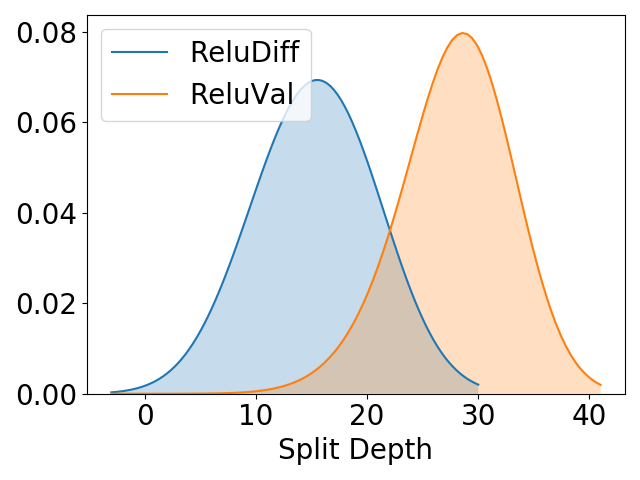
\includegraphics[width=\linewidth]{reludiff/figs/prop4_split_depth.png}
		\caption{$ \phi_4 $ max depth distribution.\label{fig:prop4_depth}}
	\end{minipage}
	\begin{minipage}[t]{0.495\linewidth}
				\captionsetup{width=0.9\textwidth}
			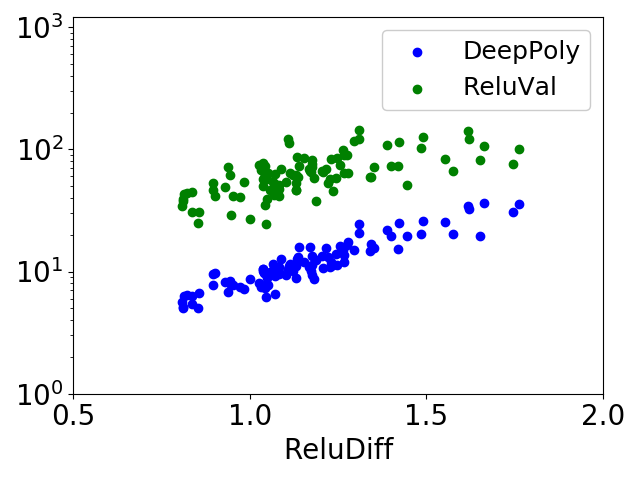
\includegraphics[width=\linewidth]{reludiff/figs/deeppoly_mnist_4_1024_compare.png}
			\caption{$\Delta $-interval on MNIST 4x1024\label{fig:deeppoly_comp}.}
	\end{minipage}%
\end{figure}

\subsubsection{MNIST}

While in ACAS Xu the input region to verify is defined by the
property, for MNIST, we must generate the input region ourselves. We
generate 200 input regions for MNIST using two methods. The first
method is based on global perturbation~\cite{SinghGPV19}. We take 100
test images, and for each one, we allow each of the pixels to be
perturbed by +/-3 gray scale units. The second method is based on
targeted pixel perturbation~\cite{GopinathPWZK19,GopinathKPB18}. We
take the same 100 test images, and for each one, we set the range of 3 random
pixels to $ [0,255] $, while the remaining 781 remain fixed.

\begin{table}
%\caption{Accuracy comparison of \diffNN{}, \ReluVal{} and \DeepPoly{} on MNIST
%networks, where network $f'$ is derived from network $f$ by rounding the weights
%to 3 significant figures, and setting  $\epsilon=2.5$.}
\centering
\caption{Accuracy comparison of the three tools on MNIST.}
\label{tbl:MNIST_accuracy}
\scalebox{1.0}{
\begin{tabular}{|l|c|cc|cc|cc|}\hline
Benchmark & Verif. & \multicolumn{2}{c|}{\diffNN{} (new)}
& \multicolumn{2}{c|}{\ReluVal{}} & \multicolumn{2}{c|}{\DeepPoly} \\
\cline{3-8}
                & problems & proved  & undet. & proved & undet. & proved & undet. \\\hline
\hline

3x100-global     & 100      & 100     &   0    &   47    & 53     & 34    & 66     \\\hline
2x512-global     & 100      & 100     &   0    &   0    & 100     & 0    & 100     \\\hline
4x1024-global    & 100      & 22     &  78    &   0    & 100     & 0   & 100      \\\hline
\hline
3x100-3-pixel     & 100     & 100     &   0    &   100    & 0     & 100    & 0     \\\hline
2x512-3-pixel     & 100     & 100     &   0    &   100    & 0     & 80   & 20     \\\hline
4x1024-3-pixel    & 100     & 100     &  0    &   97    & 3     & 100   & 0      \\\hline


\end{tabular}
}
\end{table}

\begin{table}
%\caption{Efficiency comparison of \diffNN{}, \ReluVal{} and \DeepPoly{} on MNIST
%networks, where network $f'$ is derived from network $f$ by rounding the weights
%to 3 significant figures, and setting  $\epsilon=2.5$.}
\centering
\caption{Efficiency comparison of the three tools on MNIST.}
\label{tbl:MNIST_efficiency}
\scalebox{1.0}{
\begin{tabular}{|l|c|r|r|r|}\hline
Benchmark         & Verif.  & \multicolumn{3}{c|}{ Total Time (s) }\\\cline{3-5}
                  & problems & \diffNN{} (new) & \ReluVal{} & \DeepPoly{} \\\hline
\hline
3x100-global       &     100    &        29.47     &        95458.32          &   118823.09          \\\hline
2x512-global       &     100    &        77.83     &        180000.00          &   180000.0          \\\hline
4x1024-global      &     100    &     141604.53    &        180000.00       &      180000.0     \\\hline
\hline
3x100-3-pixel       &     100   &     23.90    &        32.60            &   163.75         \\\hline
2x512-3-pixel       &     100   &     79.24    &        715.16             &   37674.40         \\\hline
4x1024-3-pixel      &     100   &     296.59       &     92100.10          &    49042.98    \\\hline
\end{tabular}
}
\end{table}


We can again see in Tables~\ref{tbl:MNIST_accuracy}
and \ref{tbl:MNIST_efficiency} that \diffNN{} is significantly more
accurate and efficient than both \ReluVal{} and \DeepPoly{}.
%
Both competing techniques struggle to handle global perturbations even
on the small 3x100 network, let alone the larger 2x512 and 4x1024 networks.
%
On the other hand, \diffNN{} can easily handle both the 3x100 and 2x512 networks,
achieving at least 3 orders of magnitude speedup on these networks.
%
We also see a three orders of magnitude speedup on the two largest networks
for our targeted-pixel perturbation experiments.

Even though \diffNN{} begins to reach its limit in the global perturbation experiment
on the largest 4x1024 network, we point out that \diffNN{} is significantly outperforming
both \DeepPoly{} and \ReluVal{} in the accuracy of their forward passes.
%
Figure~\ref{fig:deeppoly_comp} compares the output bound verified on the
\textit{first, single} forward pass of each technique.
%
The comparison is presented as a scatter plot, where the x-axis is the
bound verified by \diffNN{}, and the y-axis is that of the competing technique.

The graph shows that \diffNN{} is nearly two orders of magnitude more accurate
than \ReluVal{} and one order of magnitude more than \DeepPoly.
%
The improvement over \DeepPoly{} especially emphasizes the promise of \diffNN{}'s
approach. This is because \diffNN{} is already outperforming \DeepPoly{}, yet it
uses a simpler \emph{concretization} approach during the forward pass, whereas
\DeepPoly{} uses a more sophisticated \emph{linear relaxation}.
%
We believe that \diffNN{} can be extended to use more accurate techniques such as
linear relaxation which would further improve the accuracy, however we leave
this as future work.


\subsubsection{HAR}

For HAR, we also created our verification problems using input
perturbation.  We take 100 concrete test inputs, and for each one, we
allow a global perturbation of +/-0.1.
%
The results are summarized in Tables~\ref{tbl:HAR_accuracy} and~\ref{tbl:HAR_efficiency}.
%
%
Again, the experimental comparison shows that \diffNN{} is
significantly more accurate and efficient.



\begin{table}
	\centering
	\caption{Accuracy comparison of the three tools on HAR.}
	\label{tbl:HAR_accuracy}
	\scalebox{1.0}{
		\begin{tabular}{|l|c|cc|cc|cc|}\hline
			Benchmark & Verif. & \multicolumn{2}{c|}{\diffNN{} (new)}
			& \multicolumn{2}{c|}{\ReluVal{}} & \multicolumn{2}{c|}{\DeepPoly} \\
			\cline{3-8}
			& problems & proved  & undet. & proved & undet. & proved & undet. \\\hline
			\hline

			1x500     & 100      & 100     &   0    &   0    &   100   &  0 &  100   \\\hline

		\end{tabular}
	}
\end{table}

\begin{table}
	\centering
	\caption{Efficiency comparison of the three tools on HAR.}
	\label{tbl:HAR_efficiency}
	\scalebox{1.0}{
		\begin{tabular}{|l|c|r|r|r|}\hline
			Benchmark         & Verif.  & \multicolumn{3}{c|}{ Total Time (s) }\\\cline{3-5}
			& problems & \diffNN{} (new) & \ReluVal{} & \DeepPoly{} \\\hline
			\hline
			1x500       &     100    &        28.79     &        180000.00   &   180000.00   \\\hline
		\end{tabular}
	}
\end{table}

\subsection{Threats to Validity}


Our method is designed for verifying neural networks typically found
in control applications, where the number of input signals is not
large. In this context, dividing the input region turns out to be a
very effective way of increasing the accuracy of interval analysis.
However, neural networks in different application domains may have
different characteristics.  Therefore, it remains an open problem
whether bi-section of individual input intervals is always an
effective way of performing refinement.


Our method is designed for feed-forward ReLU networks.  Although there
is no significant technical hurdle for it to be extended to
convolutional neural networks or other activation functions, such as
sigmoid, tanh and max-pool as shown recently by Singh et
al.~\cite{SinghGPV19}, we have not evaluated the effectiveness.
Specifically, linear relaxation can be used to handle these features
when it comes to approximating non-linear behavior.  While we use
concretization in \diffNN{}, extending it with linear relaxation is
possible~\cite{WangPWYJ18nips}. However, we leave these extensions for
future work.


%\section{Related Work}
%\label{sec:related}
%
%While there is a large and growing body of work on detecting
%adversarial examples for neural networks, they are typically based on
%heuristic search or other dynamic analysis techniques such as
%testing~\cite{CarliniW17,PeiCYJ17,TianPJR18,SunWRHKK18,WickerHK18,MaLLZG18}.
%Although they are effective in finding security vulnerabilities and
%violations of other critical properties, we consider them as being
%orthogonal to formal verification.  The reason is because these
%techniques are geared toward finding violations, as opposed to proving
%the absence of violations.
%
%
%Early work on formal verification of deep neural networks relies on
%using SMT solvers~\cite{HuangKWW17,Ehlers17}, or SMT solving
%algorithms~\cite{KatzBDJK17,KatzHIJLLSTWZDK19} designed for
%efficiently reasoning about constraints from the ReLU activation
%function. Along this line, a state-of-the-art tool
%is \Reluplex{}~\cite{KatzBDJK17}.  In theory, these SMT solver based
%techniques can solve the neural network verification problem in a
%sound and complete fashion, i.e., returning a proof if and only if the
%network satisfies the property.  In practice, however, their
%scalability is often limited and they may run out of time for larger
%networks.
%
%
%Another line of work on verification of deep neural networks is based
%on interval analysis, which can be more scalable than
%SMT solver based techniques~\cite{WangPWYJ18}.  They compute
%conservative bounds on the value ranges of the neurons and output
%signals for an input region of interest.  They also exploit the fact
%that neural networks are Lipschitz continuous~\cite{RuanHK18} to
%ensure that the interval analysis results are
%sound.  \ReluVal{}~\cite{WangPWYJ18} and \DeepPoly{}~\cite{SinghGPV19}
%are two representatives, among other similar
%tools~\cite{WangPWYJ18nips,SinghGPV19iclr,MirmanGV18,GehrMDTCV18,FischerBDGZV19}.
%
%
%
%In addition to formal verification, there are techniques for
%evaluating and certifying the robustness of neural
%networks~\cite{BastaniILVNC16,CarliniW17,WengZCSHDBD18,DvijothamSGMK18}
%or certified defense against adversarial
%examples~\cite{RaghunathanSL18,WongK18}.
%%
%However, neither they nor the existing verification techniques
%were designed for \emph{differential verification} of two closely
%related neural networks, which is the focus of this paper.
%%
%%
%As shown by the examples in Section~\ref{sec:motivation} and the
%experimental results in Section~\ref{sec:experiment}, directly
%applying these techniques to differential verification is often
%extremely inefficient.  In contrast, our method is designed
%specifically for solving the differential verification problem efficiently.





At a higher level, our method relies on symbolic interval analysis,
which can be viewed as a specific form of abstract
interpretation~\cite{CousotC77}.  While the abstract interpretation
framework allows approximations to be performed in a more general way,
e.g., using relational abstract domains~\cite{Mine04} such as the
octagon~\cite{Mine01} and polyhedral~\cite{CousotH78} domains, so far,
it has not be adequately explored.  We plan to explore the use of
these abstract domains as part
of the future work.



Finally, the term \textit{differential verification} has been used
in the context of verifying a new version of a program with
respect to a previous version, which is treated as an ``oracle''~\cite{DAC13}.
In a sense, the truncated network is a ``new version'' of the original
network, and the original network can be thought of as an oracle.



\section{Summary}
\label{sec:conclusion}

We have presented a new method, named \diffNN{}, for differential
verification of two closely related neural networks.  It is capable of
formally proving the accuracy of a compressed network with respect to
the original network.  Internally, \diffNN{} relies on symbolic
interval analysis to more accurately compute and propagate differences
in the values of neurons of the two networks from the input to the
output, and then relies on the gradient difference to more accurately
compute the refinement.  Our experimental comparison of \diffNN{} with
state-of-the-art formal verification techniques shows that it can often
achieve two orders of magnitude speedup and produce many more proofs.


\section{Optimization 3 Proofs}
Here we give formal proofs for the un-proven bounds in Section~\ref{sec:opt}.
As in section~\ref{sec:opt}, we rewrite Equations~\ref{eq:1} and~\ref{eq:2} as
\begin{align*}
\deq(n,d) & = \R{n + d} - \R{n}\\
\deq'(n', d) & = \R{n'} - \R{n' - d}.
\end{align*}
where $ n \in \ReluIN{\n}, n' \in \ReluIN{\np}, $ and $ d \in \ReluINdelta{\n} $.

\subsection{Upper Bound of First Case}
Recall this case is $ \LBconcrete{\ReluINdelta{\n}} \geq 0 $.
We derive the bound from Equation~\ref{eq:2} by dividing into two cases, and then combining their result
to get the lower bound.

\subsection*{Case 1: $ n' - d > 0 = n' > d $}
Based on the above constraint, we can simplify $ \deq'(n',d) $ to
\[
	\deq'(n',d) = \R{n'} - (n' - d).
\]
In addition, since we are considering the case where $ \LBconcrete{\ReluINdelta{\n}} \geq 0 $,
we have $ d \geq 0 $. Combining this with our case 1 constraint $ n' > d $,
we have
\[
	n' > d \wedge d \geq 0 \implies n' > 0.
\]
Thus, in case 1, we have that $ \deq'(n',d) $ is just
\[
	\deq'(n',d) = n' - (n' - d) = d.
\]

We also note that $ n' > 0 $ means that
\[
n' > d \iff max(0, n') > d
\]
because $ n' > 0 $ means that $ max(0, n') = n' $. We use this fact when we combine the two cases.

\subsection*{Case 2: $ n' - d \leq 0 = n' \leq d $}
The above constraint allows us to simplify $ \deq'(n',d) $ to
\[
	\deq'(n',d) = \R{n'} - 0 = \R{n'} = max(0, n').
\]
We also note that under our constraints we have
\[
n' \leq d \iff max(0, n') \leq d,
\]
which we will use when we combine the cases. To prove this, first observe that
\[
0 \leq d \wedge n' \leq d \implies max(0, n') \leq d.
\]
That is, if $ d $ is greater-than-or-equal to both 0 and $ n' $, then clearly
it is greater-than-or-equal to the max of the two. And for the other way,
\[
max(0, n') \leq d \implies  n' \leq d.
\]
That is, if $ d $ is greater-than-or-equal to the max of 0 and $ n' $, then clearly
it is greater-than-or-equal to $ n' $.

\subsection*{Combing the Two Cases}
Combining our two cases, we get the function
\[
	\deq'(n',d) = \begin{cases}
	d & n' > d\\
	max(0, n') & n' \leq d
	\end{cases}
\]
and then substituting with the equations we derived at the end of case 1 and 2, we get
\[
\deq'(n',d) = \begin{cases}
d & max(0, n') > d\\
max(0, n') & max(0, n') \leq d
\end{cases} = min(max(0, n'), d)
\]
Since the upper bound of both $ min() $ and $ max() $ occur when we take the upper bounds of their input variables, we get that the upper bound of $ \deq'(n',d) $ is
\begin{align*}
min(max(0, \UBconcrete{\ReluIN{\np}}), \UBconcrete{\ReluINdelta{\n}})\\
= min(\UBconcrete{\ReluIN{\np}}, \UBconcrete{\ReluINdelta{\n}}).
\end{align*}
We can remove the $ max() $ function because $ \np $ is non-linear, so
$ \UBconcrete{\ReluIN{\np}} > 0 $.


\subsection{Lower Bound of Second Case}
Recall this case is $ \UBconcrete{\ReluINdelta{\n}} \leq 0 $. We derive the lower bound from Equation~\ref{eq:1} by dividing into two cases. The proof is symmetric to the previous case.
\subsection*{Case 1: $ n + d > 0 = n > -d = d > -n $}
In this case, we can immediately simplify
\[
	\deq(n,d) = n + d - \R{n}.
\]
Then, since $ \UBconcrete{\ReluINdelta{\n}} \leq 0 $ implies $ d \leq 0 = -d \geq 0 $,
we can use our case 1 constraint $ n > -d $ to derive
\[
	n > -d \wedge -d \geq 0 \implies n > 0.
\]
Thus we can further simplify
\[
	\deq(n,d) = n + d - n = d.
\]

We also note that $ n > 0 = -n < 0 \implies min(0, -n) = -n $, so we also have
\[
	d > -n \iff d > min(0, -n).
\]
We use this fact when combining the two cases.

\subsection*{Case 2: $ n + d \leq 0 = d \leq -n $}
In this case, we can immediately simplify
\[
	\deq(n,d) = 0 - \R{n} = -max(0, n) = min(0, -n).
\]
We also not here that
\[
	d \leq -n \wedge d \leq 0 \iff d \leq min(0, -n).
\]
We use this fact when combining the two cases.

\subsection*{Combining the Cases}
Combing our two cases, we get the function
\[
	\deq(n,d) = \begin{cases}
	d & d > -n\\
	min(0, -n) & d \leq -n
	\end{cases}
\]
and rewriting this equation using the inequalities we derived at the end of case 1 and 2
we get
\[
\deq(n,d) = \begin{cases}
d & d > min(0, -n)\\
min(0, -n) & d \leq min(0, -n)
\end{cases} = max(d, min(0, -n)).
\]
Since the lower bound of both $ min() $ and $ max() $ occur when we minimize their inputs, we get the lower bound of $ \deq(n,d) $ is
\begin{align*}
max(\LBconcrete{\ReluINdelta{\n}}, min(0, -\UBconcrete{\ReluIN{\n}}))\\
= max(\LBconcrete{\ReluINdelta{\n}}, -\UBconcrete{\ReluIN{\n}}).
\end{align*}
We can remove the $ min() $ function because $ \n $ is non-linear so $ -\UBconcrete{\ReluIN{\n}} < 0 $.

\subsection{Lower Bound of Third Case}
Recall this case is $ \LBconcrete{\ReluINdelta{\n}} < 0 < \UBconcrete{\ReluINdelta{\n}} $. We derive the lower bound from Equation~\ref{eq:1}. We divide into two cases and then combine them as done previously.

\subsection*{Case 1: $ n + d > 0 = d > -n $}
$ \deq(n,d) $ simplifies to
\[
	\deq(n,d) = n + d - \R{n}.
\]
We further divide into two sub-cases.

\subsection*{Case 1.1: $ n > 0 $}
$ \deq(n,d) $ further simplifies to
\[
	\deq(n,d) = n + d - n = d.
\]
Since we only care about the lower bound, observe that the lower bound of
case 1.1 occurs when we take the \textit{minimum} value of $ d $, which is \textit{always} less than 0.

\subsection*{Case 1.2: $ n \leq 0 $}
$ \deq(n,d) $ further simplifies to
\[
	\deq(n,d) = n + d - 0 = n + d.
\]
Observe that the lower bound cannot be less than 0 in case 1.2 because of the case 1 constraint.
This means the lower bound \textit{always} occurs in case 1.1, so we can safely ignore case 1.2. (But we emphasize this \textit{only} applies when evaluating $ \deq(n,d) $ for the lower bound).

\subsection*{Case 2: $ n + d \leq 0 = d \leq -n $}
$ \deq(n,d) $ further simplifies to
\[
	\deq(n,d) = 0 - \R{n} = -\R{n}.
\]
We consider the two cases of this function.
\subsection*{Case 2.1: $ n > 0 $}
$ \deq(n,d) $ becomes
\[
	\deq(n,d) = -n.
\]
The minimum value here occurs at the upper bound of $ n $, which is \textit{always} less than 0 because $ \n $ is non-linear.

\subsection*{Case 2.2: $ n \leq 0 $}
$ \deq(n,d) = 0 $ in this case. Since the lower bound of case 2.1 is \textit{always} less than 0, the minimum value will never occur in this case, so we can safely ignore it.


\subsection*{Combining the Cases}
We've shown that the minimum value occurs in either case 1.1 or case 2.1, which gives us the function (however only for the \textit{minimum} value and not the maximum)
\[
\deq(n,d) = \begin{cases}
d & d > -n\\
-n & d \leq -n
\end{cases} = max(-n,d).
\]
Evaluating this function for its lower bounds gives us
\[
 max(-\UBconcrete{\ReluIN{\n}}, \LBconcrete{\ReluINdelta{\n}}).
\]

\subsection{Upper Bound of Third Case}
Recall this case is $ \LBconcrete{\ReluINdelta{\n}} < 0 < \UBconcrete{\ReluINdelta{\n}} $. We derive the upper bound from Equation~\ref{eq:2}. We divide into two cases and then combine them as done previously. This proof mirrors the proof for the lower bound of the third case.

\subsection*{Case 1: $ n' - d > 0 = n' > d $}
$ \deq'(n',d) $ simplifies to
\[
\deq'(n',d) = \R{n'} - n' + d.
\]
We further divide into two sub-cases.

\subsection*{Case 1.1: $ n' > 0 $}
$ \deq'(n',d) $ further simplifies to
\[
\deq'(n',d) = n' - n' + d = d.
\]
Since we only care about the upper bound, observe that the upper bound of
case 1.1 occurs when we take the \textit{maximum} value of $ d $, which is always greater than 0.

\subsection*{Case 1.2: $ n' \leq 0 $}
$ \deq'(n',d) $ further simplifies to
\[
\deq'(n',d) = 0 - n' + d = -n' + d.
\]
Our case 1 constraint $ n' - d > 0 = 0 > -n' + d $ implies the upper bound in case 1.2
can be no greater than 0. This means the upper bound $ \deq'(n',d) $ always occurs in case 1.1, so we
can ignore case 1.2.

\subsection*{Case 2: $ n' - d \leq 0 = n' \leq d $}
$ \deq'(n',d) $ further simplifies to
\[
\deq'(n',d) = \R{n'} - 0 = \R{n'}.
\]
We consider the two cases of this function.
\subsection*{Case 2.1: $ n' > 0 $}
$ \deq'(n',d) $ becomes
\[
	\deq'(n',d) = n',
\]
which has its maximum value at the upper bound of $ n' $.

\subsection*{Case 2.2: $ n' \leq 0 $}
$ \deq(n,d) = 0 $ in this case. Since the upper bound of $ n' $ is greater than 0, the maximum value will never occur in this case, so we can safely ignore it.


\subsection*{Combining the Cases}
We've shown that the maximum value occurs in either case 1.1 or case 2.1, which gives us the function (only for the \textit{maximum} value and not the minimum)
\[
\deq'(n',d) = \begin{cases}
d & n' > d\\
n' & n' \leq d
\end{cases} = min(n',d).
\]
Evaluating this function for its upper bound gives us

\[
	min(\UBconcrete{\ReluIN{\np}}, \UBconcrete{\ReluINdelta{\n}}).
\]





\chapter{Symbolic Approximations for the Difference}
\label{ch:neurodiff}
\declarecommand{\Name}{\textsc{NeuroDiff}}
\declarecommand{\ReluDiffP}{\textsc{ReluDiff+}}
\declarecommand{\ReluDiff}{\textsc{ReluDiff}}

\declarecommand{\ReluVal}{\textsc{ReluVal}}
\declarecommand{\DeepPoly}{\textsc{DeepPoly}}

\declarecommand{\Reluplex}{\textsc{Reluplex}}
\declarecommand{\Neurify}{\textsc{Neurify}}
\declarecommand{\RefineZono}{\textsc{RefineZono}}

\declarecommand{\nj}[0]{n_{k,j}}
\declarecommand{\n}[2]{n_{#1,#2}}
\declarecommand{\np}[2]{n'_{#1,#2}}
\declarecommand{\npj}[0]{n'_{k,j}}
\declarecommand{\nd}[2]{\Delta_{#1,#2}}
\declarecommand{\ndj}{\Delta_{k,j}}
\declarecommand{\W}[3]{W_{#1}[#2,#3]}
\declarecommand{\Wp}[3]{W_{#1}'[#2,#3]}
\declarecommand{\Wk}[1]{W_{#1}}
\declarecommand{\Wd}[3]{W_{#1}^\Delta[#2,#3]}

\declarecommand{\IntIn}[1]{S^{in}(#1)}
\declarecommand{\IntOut}[1]{S(#1)}

\declarecommand{\relu}[1]{ReLU(#1)}

\declarecommand{\UBEq}[1]{\mathsf{UB}(#1)}
\declarecommand{\LBEq}[1]{\mathsf{LB}(#1)}
\declarecommand{\UBU}[1]{\overline{\mathsf{UB}}(#1)}
\declarecommand{\UBL}[1]{\underline{\mathsf{UB}}(#1)}
\declarecommand{\LBL}[1]{\underline{\mathsf{LB}}(#1)}
\declarecommand{\LBU}[1]{\overline{\mathsf{LB}}(#1)}



\theoremstyle{plain}
\newtheorem{thm}{Theorem}
\newtheorem{lemma}{Lemma}

\newtheoremstyle{case}{}{}{}{}{}{:}{ }{}
\theoremstyle{case}
\newtheorem{case}{Case}

%\subsubsection{Need for differential verification}
There is a growing need for rigorous analysis techniques that can
compare the behaviors of two or more neural networks trained for the
same task. For example, such techniques have applications in
better understanding the representations learned by different
networks~\cite{wang2018towards}, and finding inputs where networks
disagree~\cite{xie2019diffchaser}.
%
The need is further motivated by the increasing use of neural network
compression~\cite{HanMD16} -- a technique that alters the network's
parameters to reduce its energy and computational cost -- where
we \textit{expect} the compressed network to be functionally
equivalent to the original network.
%
In safety-critical systems where a single instance of misbehavior can
lead to catastrophe, having \textit{formal guarantees} on the
equivalence of the original and compressed networks is
highly desirable.


%\subsubsection{Limitations of existing methods}
Unfortunately, most work aimed at verifying or testing neural networks
does not provide formal guarantees on their equivalence.  For example,
testing techniques geared toward \emph{refutation} can provide inputs
where a single network misbehaves~\cite{ma2018deepgauge,
xie2019deephunter, SunWRHKK18, TianPJR18, odena2018tensorfuzz} or
multiple networks disagree~\cite{xie2019diffchaser,PeiCYJ17,MaLLZG18},
but they do not guarantee the absence of misbehaviors or disagreements.
%
While techniques geared toward \emph{verification} can prove safety or
robustness properties of a single
network~\cite{HuangKWW17,Ehlers17,KatzHIJLLSTWZDK19,RuanHK18,
WangPWYJ18nips,SinghGPV19iclr,MirmanGV18,GehrMDTCV18,FischerBDGZV19},
they lack crucial information needed to prove the equivalence of
multiple networks.
%
One exception is the \ReluDiff{} tool of Paulsen et
al.~\cite{paulsen2020reludiff}, which computes a sound approximation of the
difference of two neural networks, a problem known as
\textit{differential verification}.  While \ReluDiff{} performs
better than other techniques, the overly conservative approximation it
computes often causes both accuracy and efficiency to suffer.


%\subsubsection{Our main contributions}
To overcome these problems, we propose \Name{}, a new \emph{symbolic}
and \emph{fine-grained} approximation technique that significantly increases the
accuracy of differential verification while achieving many
orders-of-magnitude speedup.
%
\Name{} has two key contributions.  The first contribution is the development
of \emph{convex approximations}, a fine-grained approximation technique
for bounding the output difference of neurons for all possible inputs,
which drastically improves over the
coarse-grained \emph{concretizations} used by \ReluDiff{}.
%
The second contribution is judiciously introducing symbolic variables
to represent neurons in hidden layers whose difference bounds have
accumulated significant approximation error.
%
These two techniques are also complementary, i.e., when combined, the
benefit is significantly greater than the sum of their individual
benefits.



\begin{figure}[t]
	\centering
\scalebox{1.25}{

\tikzset{every picture/.style={line width=0.75pt}} %set default line width to 0.75pt

\begin{tikzpicture}[x=0.75pt,y=0.75pt,yscale=-1,xscale=1]
%uncomment if require: \path (0,300); %set diagram left start at 0, and has height of 300

%Rounded Rect [id:dp4236892252286144]
\draw  [fill={rgb, 255:red, 252; green, 202; blue, 120 }  ,fill opacity=0.5 ] (112,65.85) .. controls (112,62.62) and (114.62,60) .. (117.85,60) -- (164.15,60) .. controls (167.38,60) and (170,62.62) .. (170,65.85) -- (170,171.15) .. controls (170,174.38) and (167.38,177) .. (164.15,177) -- (117.85,177) .. controls (114.62,177) and (112,174.38) .. (112,171.15) -- cycle ;
%Shape: Circle [id:dp7068459723221313]
\draw   (123.61,89.44) .. controls (123.61,85.33) and (126.94,82) .. (131.06,82) .. controls (135.17,82) and (138.5,85.33) .. (138.5,89.44) .. controls (138.5,93.56) and (135.17,96.89) .. (131.06,96.89) .. controls (126.94,96.89) and (123.61,93.56) .. (123.61,89.44) -- cycle ;
%Shape: Circle [id:dp10436586105910262]
\draw   (143.61,89.44) .. controls (143.61,85.33) and (146.94,82) .. (151.06,82) .. controls (155.17,82) and (158.5,85.33) .. (158.5,89.44) .. controls (158.5,93.56) and (155.17,96.89) .. (151.06,96.89) .. controls (146.94,96.89) and (143.61,93.56) .. (143.61,89.44) -- cycle ;
%Shape: Circle [id:dp04586875504356169]
\draw   (113.61,114.56) .. controls (113.61,110.44) and (116.94,107.11) .. (121.06,107.11) .. controls (125.17,107.11) and (128.5,110.44) .. (128.5,114.56) .. controls (128.5,118.67) and (125.17,122) .. (121.06,122) .. controls (116.94,122) and (113.61,118.67) .. (113.61,114.56) -- cycle ;
%Shape: Circle [id:dp23529117657421317]
\draw   (133.61,114.56) .. controls (133.61,110.44) and (136.94,107.11) .. (141.06,107.11) .. controls (145.17,107.11) and (148.5,110.44) .. (148.5,114.56) .. controls (148.5,118.67) and (145.17,122) .. (141.06,122) .. controls (136.94,122) and (133.61,118.67) .. (133.61,114.56) -- cycle ;
%Shape: Circle [id:dp18975621582850755]
\draw   (153.61,114.56) .. controls (153.61,110.44) and (156.94,107.11) .. (161.06,107.11) .. controls (165.17,107.11) and (168.5,110.44) .. (168.5,114.56) .. controls (168.5,118.67) and (165.17,122) .. (161.06,122) .. controls (156.94,122) and (153.61,118.67) .. (153.61,114.56) -- cycle ;
%Straight Lines [id:da39358625060202257]
\draw    (131.06,96.89) -- (121.06,107.11) ;
%Straight Lines [id:da7050149301027024]
\draw    (131.06,96.89) -- (141.06,107.11) ;
%Straight Lines [id:da078846190833607]
\draw    (131.06,96.89) -- (161.06,107.11) ;
%Straight Lines [id:da2611151157782621]
\draw    (151.06,96.89) -- (161.06,107.11) ;
%Straight Lines [id:da854791249594143]
\draw    (151.06,96.89) -- (141.06,107.11) ;
%Straight Lines [id:da003907601781767633]
\draw    (151.06,96.89) -- (121.06,107.11) ;
%Shape: Circle [id:dp5156337693032028]
\draw   (158.5,164.56) .. controls (158.5,168.67) and (155.17,172) .. (151.06,172) .. controls (146.94,172) and (143.61,168.67) .. (143.61,164.56) .. controls (143.61,160.44) and (146.94,157.11) .. (151.06,157.11) .. controls (155.17,157.11) and (158.5,160.44) .. (158.5,164.56) -- cycle ;
%Shape: Circle [id:dp06607101355690326]
\draw   (138.5,164.56) .. controls (138.5,168.67) and (135.17,172) .. (131.06,172) .. controls (126.94,172) and (123.61,168.67) .. (123.61,164.56) .. controls (123.61,160.44) and (126.94,157.11) .. (131.06,157.11) .. controls (135.17,157.11) and (138.5,160.44) .. (138.5,164.56) -- cycle ;
%Shape: Circle [id:dp10601416223357618]
\draw   (168.5,139.44) .. controls (168.5,143.56) and (165.17,146.89) .. (161.06,146.89) .. controls (156.94,146.89) and (153.61,143.56) .. (153.61,139.44) .. controls (153.61,135.33) and (156.94,132) .. (161.06,132) .. controls (165.17,132) and (168.5,135.33) .. (168.5,139.44) -- cycle ;
%Shape: Circle [id:dp25720293065397004]
\draw   (148.5,139.44) .. controls (148.5,143.56) and (145.17,146.89) .. (141.06,146.89) .. controls (136.94,146.89) and (133.61,143.56) .. (133.61,139.44) .. controls (133.61,135.33) and (136.94,132) .. (141.06,132) .. controls (145.17,132) and (148.5,135.33) .. (148.5,139.44) -- cycle ;
%Shape: Circle [id:dp4093542080553124]
\draw   (128.5,139.44) .. controls (128.5,143.56) and (125.17,146.89) .. (121.06,146.89) .. controls (116.94,146.89) and (113.61,143.56) .. (113.61,139.44) .. controls (113.61,135.33) and (116.94,132) .. (121.06,132) .. controls (125.17,132) and (128.5,135.33) .. (128.5,139.44) -- cycle ;
%Straight Lines [id:da8322313642706787]
\draw    (151.06,157.11) -- (161.06,146.89) ;
%Straight Lines [id:da4076421006538775]
\draw    (151.06,157.11) -- (141.06,146.89) ;
%Straight Lines [id:da22036650281611347]
\draw    (151.06,157.11) -- (121.06,146.89) ;
%Straight Lines [id:da5955438584611725]
\draw    (131.06,157.11) -- (121.06,146.89) ;
%Straight Lines [id:da6153976114126399]
\draw    (131.06,157.11) -- (141.06,146.89) ;
%Straight Lines [id:da9953813996835473]
\draw    (131.06,157.11) -- (161.06,146.89) ;

%Straight Lines [id:da23986906826746157]
\draw    (121.06,122) -- (141.06,132) ;
%Straight Lines [id:da2936393327105673]
\draw    (121.06,122) -- (161.06,132) ;
%Straight Lines [id:da5774592223000948]
\draw    (141.06,122) -- (121.06,132) ;
%Straight Lines [id:da027247136169882613]
\draw    (141.06,122) -- (141.06,132) ;
%Straight Lines [id:da2078286476738037]
\draw    (141.06,122) -- (161.06,132) ;
%Straight Lines [id:da07067307391973043]
\draw    (161.06,122) -- (161.06,132) ;
%Straight Lines [id:da5480660909270823]
\draw    (161.06,122) -- (141.06,132) ;
%Straight Lines [id:da6293253437621619]
\draw    (161.06,122) -- (121.06,132) ;
%Straight Lines [id:da7407175241217754]
\draw    (121.06,122) -- (121.06,132) ;

%Rounded Rect [id:dp2355420157466821]
\draw  [fill={rgb, 255:red, 252; green, 202; blue, 120 }  ,fill opacity=0.5 ] (50,182.02) .. controls (50,180.9) and (50.9,180) .. (52.02,180) -- (105.98,180) .. controls (107.1,180) and (108,180.9) .. (108,182.02) -- (108,197.98) .. controls (108,199.1) and (107.1,200) .. (105.98,200) -- (52.02,200) .. controls (50.9,200) and (50,199.1) .. (50,197.98) -- cycle ;
%Rounded Rect [id:dp39333818742980176]
\draw  [fill={rgb, 255:red, 144; green, 195; blue, 255 }  ,fill opacity=0.5 ] (180,74.13) .. controls (180,66.33) and (186.33,60) .. (194.13,60) -- (355.87,60) .. controls (363.67,60) and (370,66.33) .. (370,74.13) -- (370,185.87) .. controls (370,193.67) and (363.67,200) .. (355.87,200) -- (194.13,200) .. controls (186.33,200) and (180,193.67) .. (180,185.87) -- cycle ;
%Rounded Rect [id:dp15859389295109172]
\draw   (246,70.5) .. controls (253.73,70.5) and (260,76.77) .. (260,84.5) -- (260,176) .. controls (260,183.73) and (253.73,190) .. (246,190) -- (204,190) .. controls (196.27,190) and (190,183.73) .. (190,176) -- (190,84.5) .. controls (190,76.77) and (196.27,70.5) .. (204,70.5) -- cycle ;
%Straight Lines [id:da09167228503135971]
\draw    (170,100) -- (187,100) ;
\draw [shift={(190,100)}, rotate = 180] [fill={rgb, 255:red, 0; green, 0; blue, 0 }  ][line width=0.08]  [draw opacity=0] (8.93,-4.29) -- (0,0) -- (8.93,4.29) -- cycle    ;
%Straight Lines [id:da15082942023264767]
\draw    (170,190) -- (189.35,102.93) ;
\draw [shift={(190,100)}, rotate = 462.53] [fill={rgb, 255:red, 0; green, 0; blue, 0 }  ][line width=0.08]  [draw opacity=0] (8.93,-4.29) -- (0,0) -- (8.93,4.29) -- cycle    ;
%Rounded Rect [id:dp19836331083326175]
\draw  [fill={rgb, 255:red, 252; green, 202; blue, 120 }  ,fill opacity=0.5 ] (112,182.02) .. controls (112,180.9) and (112.9,180) .. (114.02,180) -- (167.98,180) .. controls (169.1,180) and (170,180.9) .. (170,182.02) -- (170,197.98) .. controls (170,199.1) and (169.1,200) .. (167.98,200) -- (114.02,200) .. controls (112.9,200) and (112,199.1) .. (112,197.98) -- cycle ;
%Rounded Rect [id:dp3414447171885684]
\draw   (190,163.86) .. controls (190,156.2) and (196.2,150) .. (203.86,150) -- (246.14,150) .. controls (253.8,150) and (260,156.2) .. (260,163.86) -- (260,176.14) .. controls (260,183.8) and (253.8,190) .. (246.14,190) -- (203.86,190) .. controls (196.2,190) and (190,183.8) .. (190,176.14) -- cycle ;
%Rounded Rect [id:dp7331605414728447]
\draw   (190,123.36) .. controls (190,115.7) and (196.2,109.5) .. (203.86,109.5) -- (246.14,109.5) .. controls (253.8,109.5) and (260,115.7) .. (260,123.36) -- (260,135.64) .. controls (260,143.3) and (253.8,149.5) .. (246.14,149.5) -- (203.86,149.5) .. controls (196.2,149.5) and (190,143.3) .. (190,135.64) -- cycle ;
%Rounded Rect [id:dp724286819012004]
\draw   (356,170) .. controls (358.21,170) and (360,171.79) .. (360,174) -- (360,186) .. controls (360,188.21) and (358.21,190) .. (356,190) -- (294,190) .. controls (291.79,190) and (290,188.21) .. (290,186) -- (290,174) .. controls (290,171.79) and (291.79,170) .. (294,170) -- cycle ;
%Rounded Rect [id:dp8526981920637079]
\draw   (355.84,125) .. controls (358.14,125) and (360,126.86) .. (360,129.16) -- (360,141.62) .. controls (360,143.92) and (358.14,145.78) .. (355.84,145.78) -- (294.16,145.78) .. controls (291.86,145.78) and (290,143.92) .. (290,141.62) -- (290,129.16) .. controls (290,126.86) and (291.86,125) .. (294.16,125) -- cycle ;
%Rounded Rect [id:dp6803009958438129]
\draw   (354,70) .. controls (357.31,70) and (360,72.69) .. (360,76) -- (360,94) .. controls (360,97.31) and (357.31,100) .. (354,100) -- (296,100) .. controls (292.69,100) and (290,97.31) .. (290,94) -- (290,76) .. controls (290,72.69) and (292.69,70) .. (296,70) -- cycle ;
%Straight Lines [id:da323377208231176]
\draw    (300,170) -- (300,149) ;
\draw [shift={(300,146)}, rotate = 450] [fill={rgb, 255:red, 0; green, 0; blue, 0 }  ][line width=0.08]  [draw opacity=0] (8.93,-4.29) -- (0,0) -- (8.93,4.29) -- cycle    ;
%Straight Lines [id:da9479303756560082]
\draw    (301,125) -- (301,103) ;
\draw [shift={(301,100)}, rotate = 450] [fill={rgb, 255:red, 0; green, 0; blue, 0 }  ][line width=0.08]  [draw opacity=0] (8.93,-4.29) -- (0,0) -- (8.93,4.29) -- cycle    ;
%Straight Lines [id:da32236695764284484]
\draw    (260,180) -- (287,180) ;
\draw [shift={(290,180)}, rotate = 180] [fill={rgb, 255:red, 0; green, 0; blue, 0 }  ][line width=0.08]  [draw opacity=0] (8.93,-4.29) -- (0,0) -- (8.93,4.29) -- cycle    ;
%Straight Lines [id:da551116351892766]
\draw    (360,135) -- (397,135) ;
\draw [shift={(400,135)}, rotate = 180] [fill={rgb, 255:red, 0; green, 0; blue, 0 }  ][line width=0.08]  [draw opacity=0] (8.93,-4.29) -- (0,0) -- (8.93,4.29) -- cycle    ;
%Rounded Rect [id:dp9869780674255966]
\draw  [fill={rgb, 255:red, 252; green, 202; blue, 120 }  ,fill opacity=0.5 ] (50,65.85) .. controls (50,62.62) and (52.62,60) .. (55.85,60) -- (102.15,60) .. controls (105.38,60) and (108,62.62) .. (108,65.85) -- (108,171.15) .. controls (108,174.38) and (105.38,177) .. (102.15,177) -- (55.85,177) .. controls (52.62,177) and (50,174.38) .. (50,171.15) -- cycle ;
%Shape: Circle [id:dp8539692235458093]
\draw   (61.61,89.44) .. controls (61.61,85.33) and (64.94,82) .. (69.06,82) .. controls (73.17,82) and (76.5,85.33) .. (76.5,89.44) .. controls (76.5,93.56) and (73.17,96.89) .. (69.06,96.89) .. controls (64.94,96.89) and (61.61,93.56) .. (61.61,89.44) -- cycle ;
%Shape: Circle [id:dp1487342990764624]
\draw   (81.61,89.44) .. controls (81.61,85.33) and (84.94,82) .. (89.06,82) .. controls (93.17,82) and (96.5,85.33) .. (96.5,89.44) .. controls (96.5,93.56) and (93.17,96.89) .. (89.06,96.89) .. controls (84.94,96.89) and (81.61,93.56) .. (81.61,89.44) -- cycle ;
%Shape: Circle [id:dp35573619874650775]
\draw   (51.61,114.56) .. controls (51.61,110.44) and (54.94,107.11) .. (59.06,107.11) .. controls (63.17,107.11) and (66.5,110.44) .. (66.5,114.56) .. controls (66.5,118.67) and (63.17,122) .. (59.06,122) .. controls (54.94,122) and (51.61,118.67) .. (51.61,114.56) -- cycle ;
%Shape: Circle [id:dp43998418948198004]
\draw   (71.61,114.56) .. controls (71.61,110.44) and (74.94,107.11) .. (79.06,107.11) .. controls (83.17,107.11) and (86.5,110.44) .. (86.5,114.56) .. controls (86.5,118.67) and (83.17,122) .. (79.06,122) .. controls (74.94,122) and (71.61,118.67) .. (71.61,114.56) -- cycle ;
%Shape: Circle [id:dp11364870191253851]
\draw   (91.61,114.56) .. controls (91.61,110.44) and (94.94,107.11) .. (99.06,107.11) .. controls (103.17,107.11) and (106.5,110.44) .. (106.5,114.56) .. controls (106.5,118.67) and (103.17,122) .. (99.06,122) .. controls (94.94,122) and (91.61,118.67) .. (91.61,114.56) -- cycle ;
%Straight Lines [id:da5311768222051036]
\draw    (69.06,96.89) -- (59.06,107.11) ;
%Straight Lines [id:da8245862905976873]
\draw    (69.06,96.89) -- (79.06,107.11) ;
%Straight Lines [id:da9037048113348528]
\draw    (69.06,96.89) -- (99.06,107.11) ;
%Straight Lines [id:da6775367181725077]
\draw    (89.06,96.89) -- (99.06,107.11) ;
%Straight Lines [id:da20764974600729147]
\draw    (89.06,96.89) -- (79.06,107.11) ;
%Straight Lines [id:da4787036285423938]
\draw    (89.06,96.89) -- (59.06,107.11) ;
%Shape: Circle [id:dp6787178527201608]
\draw   (96.5,164.56) .. controls (96.5,168.67) and (93.17,172) .. (89.06,172) .. controls (84.94,172) and (81.61,168.67) .. (81.61,164.56) .. controls (81.61,160.44) and (84.94,157.11) .. (89.06,157.11) .. controls (93.17,157.11) and (96.5,160.44) .. (96.5,164.56) -- cycle ;
%Shape: Circle [id:dp8189142658483558]
\draw   (76.5,164.56) .. controls (76.5,168.67) and (73.17,172) .. (69.06,172) .. controls (64.94,172) and (61.61,168.67) .. (61.61,164.56) .. controls (61.61,160.44) and (64.94,157.11) .. (69.06,157.11) .. controls (73.17,157.11) and (76.5,160.44) .. (76.5,164.56) -- cycle ;
%Shape: Circle [id:dp21275076334366427]
\draw   (106.5,139.44) .. controls (106.5,143.56) and (103.17,146.89) .. (99.06,146.89) .. controls (94.94,146.89) and (91.61,143.56) .. (91.61,139.44) .. controls (91.61,135.33) and (94.94,132) .. (99.06,132) .. controls (103.17,132) and (106.5,135.33) .. (106.5,139.44) -- cycle ;
%Shape: Circle [id:dp1824568474340943]
\draw   (86.5,139.44) .. controls (86.5,143.56) and (83.17,146.89) .. (79.06,146.89) .. controls (74.94,146.89) and (71.61,143.56) .. (71.61,139.44) .. controls (71.61,135.33) and (74.94,132) .. (79.06,132) .. controls (83.17,132) and (86.5,135.33) .. (86.5,139.44) -- cycle ;
%Shape: Circle [id:dp825767248504503]
\draw   (66.5,139.44) .. controls (66.5,143.56) and (63.17,146.89) .. (59.06,146.89) .. controls (54.94,146.89) and (51.61,143.56) .. (51.61,139.44) .. controls (51.61,135.33) and (54.94,132) .. (59.06,132) .. controls (63.17,132) and (66.5,135.33) .. (66.5,139.44) -- cycle ;
%Straight Lines [id:da6766885451674735]
\draw    (89.06,157.11) -- (99.06,146.89) ;
%Straight Lines [id:da08122409377631135]
\draw    (89.06,157.11) -- (79.06,146.89) ;
%Straight Lines [id:da8441374241505181]
\draw    (89.06,157.11) -- (59.06,146.89) ;
%Straight Lines [id:da7442737845395763]
\draw    (69.06,157.11) -- (59.06,146.89) ;
%Straight Lines [id:da9566636567575862]
\draw    (69.06,157.11) -- (79.06,146.89) ;
%Straight Lines [id:da19409192754236826]
\draw    (69.06,157.11) -- (99.06,146.89) ;

%Straight Lines [id:da39227385116907143]
\draw    (59.06,122) -- (79.06,132) ;
%Straight Lines [id:da16288130182449367]
\draw    (59.06,122) -- (99.06,132) ;
%Straight Lines [id:da19810001689574364]
\draw    (79.06,122) -- (59.06,132) ;
%Straight Lines [id:da24191813694330322]
\draw    (79.06,122) -- (79.06,132) ;
%Straight Lines [id:da1525732415062876]
\draw    (79.06,122) -- (99.06,132) ;
%Straight Lines [id:da22405676573237499]
\draw    (99.06,122) -- (99.06,132) ;
%Straight Lines [id:da9334192766546668]
\draw    (99.06,122) -- (79.06,132) ;
%Straight Lines [id:da3285219924463475]
\draw    (99.06,122) -- (59.06,132) ;
%Straight Lines [id:da28988712234136327]
\draw    (59.06,122) -- (59.06,132) ;

%Straight Lines [id:da08693151331707771]
\draw    (290,80) -- (263,80) ;
\draw [shift={(260,80)}, rotate = 360] [fill={rgb, 255:red, 0; green, 0; blue, 0 }  ][line width=0.08]  [draw opacity=0] (8.93,-4.29) -- (0,0) -- (8.93,4.29) -- cycle    ;
%Straight Lines [id:da3246311983059058]
\draw    (290,90) -- (263,90) ;
\draw [shift={(260,90)}, rotate = 360] [fill={rgb, 255:red, 0; green, 0; blue, 0 }  ][line width=0.08]  [draw opacity=0] (8.93,-4.29) -- (0,0) -- (8.93,4.29) -- cycle    ;

% Text Node
\draw (53,47) node [anchor=north west][inner sep=0.75pt]   [align=left] {\small
Inputs};
% Text Node
\draw (184,48) node [anchor=north west][inner sep=0.75pt]   [align=left] {\small
NeuroDiff};
% Text Node
\draw (196,76.5) node [anchor=north west][inner sep=0.75pt]   [align=left] {\begin{minipage}[lt]{40.70935600000001pt}\setlength\topsep{0pt}
	\begin{center}
	{\small Forward}\\{\small Analysis}
	\end{center}

	\end{minipage}};
% Text Node
\draw (183,114.5) node [anchor=north west][inner sep=0.75pt]   [align=left] {\begin{minipage}[lt]{61.370000000000005pt}\setlength\topsep{0pt}
	\begin{center}
	{\scriptsize Convex}\\{\scriptsize Approximation}
	\end{center}

	\end{minipage}};
% Text Node
\draw (187.5,157) node [anchor=north west][inner sep=0.75pt]   [align=left] {\begin{minipage}[lt]{53.720000000000006pt}\setlength\topsep{0pt}
	\begin{center}
	{\scriptsize Intermediate}\\{\scriptsize Variables}
	\end{center}

	\end{minipage}};
% Text Node
\draw (296,173.5) node [anchor=north west][inner sep=0.75pt]   [align=left] {\begin{minipage}[lt]{39.848000000000006pt}\setlength\topsep{0pt}
	\begin{center}
	Check $\displaystyle \epsilon $
	\end{center}

	\end{minipage}};
% Text Node
\draw (369,125) node [anchor=north west][inner sep=0.75pt]  [font=\footnotesize] [align=left] {\begin{minipage}[lt]{16.025356000000002pt}\setlength\topsep{0pt}
	\begin{center}
	Yes
	\end{center}

	\end{minipage}};
% Text Node
\draw (397,129) node [anchor=north west][inner sep=0.75pt]  [font=\footnotesize] [align=left] {\begin{minipage}[lt]{29.931356pt}\setlength\topsep{0pt}
	\begin{center}
	Verified
	\end{center}

	\end{minipage}};
% Text Node
\draw (296.5,72) node [anchor=north west][inner sep=0.75pt]   [align=left] {\begin{minipage}[lt]{40.154pt}\setlength\topsep{0pt}
	\begin{center}
	{\footnotesize Partition $\displaystyle X$}
	\end{center}

	\end{minipage}};
% Text Node
\draw (307,111) node [anchor=north west][inner sep=0.75pt]  [font=\footnotesize] [align=left] {\begin{minipage}[lt]{13.146644000000002pt}\setlength\topsep{0pt}
	\begin{center}
	No
	\end{center}

	\end{minipage}};
% Text Node
\draw (57.56,65.5) node [anchor=north west][inner sep=0.75pt]   [align=left] {\begin{minipage}[lt]{30.498000000000005pt}\setlength\topsep{0pt}
	\begin{center}
	$ f $
	\end{center}

	\end{minipage}};
% Text Node
\draw (119.56,65.5) node [anchor=north west][inner sep=0.75pt]   [align=left] {\begin{minipage}[lt]{30.498000000000005pt}\setlength\topsep{0pt}
	\begin{center}
	$ f' $
	\end{center}

	\end{minipage}};
% Text Node
\draw (113.06,183.5) node [anchor=north west][inner sep=0.75pt]   [align=left] {\begin{minipage}[lt]{40.63pt}\setlength\topsep{0pt}
	\begin{center}
	$\displaystyle X\subseteq \mathbb{R}^{n}$
	\end{center}

	\end{minipage}};
% Text Node
\draw (73.56,186.5) node [anchor=north west][inner sep=0.75pt]   [align=left] {\begin{minipage}[lt]{8.67pt}\setlength\topsep{0pt}
	\begin{center}
	$\displaystyle \epsilon $
	\end{center}

	\end{minipage}};
% Text Node
\draw (269,67) node [anchor=north west][inner sep=0.75pt]   [align=left] {\begin{minipage}[lt]{16.127356000000002pt}\setlength\topsep{0pt}
	\begin{center}
	$\displaystyle X_{1}$
	\end{center}

	\end{minipage}};
% Text Node
\draw (269,92) node [anchor=north west][inner sep=0.75pt]   [align=left] {\begin{minipage}[lt]{16.127356000000002pt}\setlength\topsep{0pt}
	\begin{center}
	$\displaystyle X_{2}$
	\end{center}

	\end{minipage}};
% Text Node
\draw (296.5,128.83) node [anchor=north west][inner sep=0.75pt]   [align=left] {\begin{minipage}[lt]{40.732pt}\setlength\topsep{0pt}
	\begin{center}
	Proven?
	\end{center}

	\end{minipage}};


\end{tikzpicture}
}
\caption{The overall flow of \Name{}.}
\label{neurodiff:fig:diagram}
\end{figure}


%\subsubsection{Overall flow of our method}
The overall flow of \Name{} is shown in Figure~\ref{neurodiff:fig:diagram},
where it takes as input two neural networks $ f $ and $ f' $, a set of
inputs to the neural networks $ X $ defined by box intervals, and a small
constant $ \epsilon $ that quantifies the tolerance for disagreement. We assume
that $ f $ and $ f' $ have the same network topology and only differ in the
numerical values of their weights. In practice, $ f' $ could be the compressed
version of $ f $, or they could be networks constructed using the same network
topology but slightly different training data. We also note that this
assumption can support compression techniques such as weight
pruning~\cite{HanMD16} (by setting edges' weights to 0) and even neuron
removal~\cite{gokulanathan2019simplifying} (by setting all of a neuron's
incoming edge weights to 0). \Name{} then aims to prove $
\forall
x \in X. |f'(x) - f(x)| < \epsilon $. It can return
(1) \emph{verified} if a proof can be found, or
(2) \emph{undetermined} if a specified timeout is reached.


Internally, \Name{} first performs a forward analysis using symbolic
interval arithmetic to bound both the absolute value ranges of all
neurons, as in single network verification, and the difference between
the neurons of the two networks. \Name{} then checks if the difference
between the output neurons satisfies $ \epsilon $, and if so
returns \emph{verified}. Otherwise,
\Name{} uses a gradient-based refinement to partition $ X
$ into two disjoint sub regions $ X_1 $ and $ X_2 $, and attempts the
analysis again on the individual regions. Since $ X_1 $ and $ X_2 $
form independent sub-problems, we can do these analyses in parallel,
hence gaining significant speedup.
%  (a) interval arithmetic to propagate absolute value ranges
%  (b) interval arithmetic to propagate difference value ranges
%  (c) multi-threading to perform forward interval analysis
%  (d) gradient based refinement to partition input regions


%\subsubsection{Convex approximation: what's new?}
The new convex approximations used in \Name{} are significantly more
accurate than not only the coarse-grained \emph{concretizations}
in \ReluDiff{}~\cite{paulsen2020reludiff} but also the standard convex
approximations in single-network verification tools~\cite{SinghGPV19,
Singh2019krelu, WangPWYJ18nips, zhang2018efficient}.
%
While these (standard) convex approximations aim to bound the absolute
value range of $ y = \relu{x} $, where $x$ is the input of
the \textit{rectified linear unit} (ReLU) activation function, our new
convex approximations aim to bound the difference $ z = \relu{x
+ \Delta} - \relu{x} $, where $x$ and $x+\Delta$ are ReLU inputs of
two corresponding neurons.
%
This is significantly more challenging because it involves the search
of bounding planes in a three-dimensional space (defined by $x$,
$\Delta$ and $z$) as opposed to a two-dimensional space as in the
prior work.


%\subsubsection{Symbolic variables: what's new?}
The symbolic variables we judiciously add to represent values of
neurons in hidden layers should not be confused with the symbolic
inputs used by existing tools either.
%
While the use of symbolic inputs is well understood, e.g., both in
single-network verification~\cite{SinghGPV19, Singh2019krelu,
WangPWYJ18nips, zhang2018efficient} and differential
verification~\cite{paulsen2020reludiff}, this is the first time that symbolic
variables are used to substitute values of hidden neurons during
differential verification.
%
While the impact of symbolic inputs often diminishes after the first
few layers of neurons, the impact of these new symbolic variables,
when judiciously added, can be maintained in any hidden layer.


%\subsubsection{Experiments: does it work?}
We have implemented the proposed \Name{} in a tool and evaluated it on
a large set of differential verification tasks. Our benchmarks
consists of 49 networks, from applications such as aircraft collision
avoidance, image classification, and human activity recognition.  We
have experimentally compared with \ReluDiff{}~\cite{paulsen2020reludiff}, the
state-of-the-art tool which has also been shown to be superior to
\ReluVal{}~\cite{WangPWYJ18} and \DeepPoly{}~\cite{SinghGPV19} for differential
verification.
%
Our results show that \Name{} is up to 1,000X faster and 5X more
accurate.  In addition, \Name{} is able to prove many of the same properties
as \ReluDiff{} while considering much larger input regions.


To summarize, this paper makes the following contributions:
\begin{itemize}
\item
We propose new convex approximations to more accurately bound the
difference between corresponding neurons of two structurally similar
neural networks.
\item
We propose a method for judiciously introducing symbolic variables to
neurons in hidden layers to mitigate the propagation of approximation
error.
\item
We implement and evaluate the proposed technique on a large number of
differential verification tasks and demonstrate its significant speed
and accuracy gains.
\end{itemize}


The remainder of this chapter is organized as follows.  First, we
provide a brief overview of our method in Section~\ref{neurodiff:sec:overview}.
Then, we provide the technical background in
Section~\ref{neurodiff:sec:preliminary}.  Next, we present the detailed
algorithms in Section~\ref{neurodiff:sec:approach} and the experimental results
in Section~\ref{neurodiff:sec:experiment}. Finally, we summarize the contributions
of this chapter in Section~\ref{neurodiff:sec:conclusion}.



\section{Overview}
\label{neurodiff:sec:overview}

In this section, we highlight our main contributions and illustrate
the shortcomings of previous work on a motivating example.


\begin{figure}
	\centering
\scalebox{1.25}{

\tikzset{every picture/.style={line width=0.75pt}} %set default line width to 0.75pt

\begin{tikzpicture}[x=0.75pt,y=0.75pt,yscale=-1,xscale=1]
%uncomment if require: \path (0,395); %set diagram left start at 0, and has height of 395

%Shape: Circle [id:dp29452950296941915]
%\draw   (90,55) .. controls (90,41.19) and (101.19,30) .. (115,30) .. controls (128.81,30) and (140,41.19) .. (140,55) .. controls (140,68.81) and (128.81,80) .. (115,80) .. controls (101.19,80) and (90,68.81) .. (90,55) -- cycle ;
\draw (115,55) +(-25,-20) rectangle +(25,20) ;
%Shape: Circle [id:dp7730288688046164]
%\draw   (90,160) .. controls (90,146.19) and (101.19,135) .. (115,135) .. controls (128.81,135) and (140,146.19) .. (140,160) .. controls (140,173.81) and (128.81,185) .. (115,185) .. controls (101.19,185) and (90,173.81) .. (90,160) -- cycle ;
\draw (115,160) +(-25,-20) rectangle +(25,20) ;
%Shape: Circle [id:dp7848793538270885]
\draw   (190,160) .. controls (190,146.19) and (201.19,135) .. (215,135) .. controls (228.81,135) and (240,146.19) .. (240,160) .. controls (240,173.81) and (228.81,185) .. (215,185) .. controls (201.19,185) and (190,173.81) .. (190,160) -- cycle ;
%Shape: Circle [id:dp2581761932666119]
\draw   (190,55) .. controls (190,41.19) and (201.19,30) .. (215,30) .. controls (228.81,30) and (240,41.19) .. (240,55) .. controls (240,68.81) and (228.81,80) .. (215,80) .. controls (201.19,80) and (190,68.81) .. (190,55) -- cycle ;
%Shape: Circle [id:dp03162623697960232]
\draw   (290,160) .. controls (290,146.19) and (301.19,135) .. (315,135) .. controls (328.81,135) and (340,146.19) .. (340,160) .. controls (340,173.81) and (328.81,185) .. (315,185) .. controls (301.19,185) and (290,173.81) .. (290,160) -- cycle ;
%Shape: Circle [id:dp02546394024001375]
\draw   (290,55) .. controls (290,41.19) and (301.19,30) .. (315,30) .. controls (328.81,30) and (340,41.19) .. (340,55) .. controls (340,68.81) and (328.81,80) .. (315,80) .. controls (301.19,80) and (290,68.81) .. (290,55) -- cycle ;
%Shape: Circle [id:dp12084775666404268]
%\draw   (371,105) .. controls (371,91.19) and (382.19,80) .. (396,80) .. controls (409.81,80) and (421,91.19) .. (421,105) .. controls (421,118.81) and (409.81,130) .. (396,130) .. controls (382.19,130) and (371,118.81) .. (371,105) -- cycle ;
\draw (396,105) +(-25,-20) rectangle +(25,20) ;
%Straight Lines [id:da34998381745971496]
\draw    (140,160) -- (187,160) ;
\draw [shift={(190,160)}, rotate = 180] [fill={rgb, 255:red, 0; green, 0; blue, 0 }  ][line width=0.08]  [draw opacity=0] (10.72,-5.15) -- (0,0) -- (10.72,5.15) -- (7.12,0) -- cycle    ;
%Straight Lines [id:da4638805061238097]
\draw    (140,160) -- (188.71,57.71) ;
\draw [shift={(190,55)}, rotate = 475.46] [fill={rgb, 255:red, 0; green, 0; blue, 0 }  ][line width=0.08]  [draw opacity=0] (10.72,-5.15) -- (0,0) -- (10.72,5.15) -- (7.12,0) -- cycle    ;
%Straight Lines [id:da15742477491714235]
\draw    (140,55) -- (187,55) ;
\draw [shift={(190,55)}, rotate = 180] [fill={rgb, 255:red, 0; green, 0; blue, 0 }  ][line width=0.08]  [draw opacity=0] (10.72,-5.15) -- (0,0) -- (10.72,5.15) -- (7.12,0) -- cycle    ;
%Straight Lines [id:da9054930639679811]
\draw    (140,55) -- (188.71,157.29) ;
\draw [shift={(190,160)}, rotate = 244.54000000000002] [fill={rgb, 255:red, 0; green, 0; blue, 0 }  ][line width=0.08]  [draw opacity=0] (10.72,-5.15) -- (0,0) -- (10.72,5.15) -- (7.12,0) -- cycle    ;
%Straight Lines [id:da0727882271401632]
\draw    (240,160) -- (288.71,57.71) ;
\draw [shift={(290,55)}, rotate = 475.46] [fill={rgb, 255:red, 0; green, 0; blue, 0 }  ][line width=0.08]  [draw opacity=0] (10.72,-5.15) -- (0,0) -- (10.72,5.15) -- (7.12,0) -- cycle    ;
%Straight Lines [id:da02068180741540726]
\draw    (240,55) -- (288.71,157.29) ;
\draw [shift={(290,160)}, rotate = 244.54000000000002] [fill={rgb, 255:red, 0; green, 0; blue, 0 }  ][line width=0.08]  [draw opacity=0] (10.72,-5.15) -- (0,0) -- (10.72,5.15) -- (7.12,0) -- cycle    ;
%Straight Lines [id:da4941096166166473]
\draw    (340,55) -- (369.42,102.45) ;
\draw [shift={(371,105)}, rotate = 238.2] [fill={rgb, 255:red, 0; green, 0; blue, 0 }  ][line width=0.08]  [draw opacity=0] (10.72,-5.15) -- (0,0) -- (10.72,5.15) -- (7.12,0) -- cycle    ;
%Straight Lines [id:da0005753242144755921]
\draw    (340,160) -- (369.53,107.61) ;
\draw [shift={(371,105)}, rotate = 479.41] [fill={rgb, 255:red, 0; green, 0; blue, 0 }  ][line width=0.08]  [draw opacity=0] (10.72,-5.15) -- (0,0) -- (10.72,5.15) -- (7.12,0) -- cycle    ;
%Straight Lines [id:da6663993224468625]
\draw    (240,160) -- (287,160) ;
\draw [shift={(290,160)}, rotate = 180] [fill={rgb, 255:red, 0; green, 0; blue, 0 }  ][line width=0.08]  [draw opacity=0] (10.72,-5.15) -- (0,0) -- (10.72,5.15) -- (7.12,0) -- cycle    ;
%Straight Lines [id:da971612493075633]
\draw    (240,55) -- (287,55) ;
\draw [shift={(290,55)}, rotate = 180] [fill={rgb, 255:red, 0; green, 0; blue, 0 }  ][line width=0.08]  [draw opacity=0] (10.72,-5.15) -- (0,0) -- (10.72,5.15) -- (7.12,0) -- cycle    ;

% Text Node
\draw (165,43) node  [font=\normalsize] [align=left] {1.9};
% Text Node
\draw (140,90) node  [font=\normalsize] [align=left] {1.1};
% Text Node
\draw (140,120) node  [font=\normalsize] [align=left] {\mbox{-}1.9};
% Text Node
\draw (165,172.5) node  [font=\normalsize] [align=left] {1.0};
% Text Node
\draw (265,42.5) node  [font=\normalsize] [align=left] {2.1};
% Text Node
\draw (238,90) node  [font=\normalsize] [align=left] {0.9};
% Text Node
\draw (265,172.5) node  [font=\normalsize] [align=left] {1.1};
% Text Node
\draw (238,120) node  [font=\normalsize] [align=left] {\mbox{-}1.0};
% Text Node
\draw (366.5,69) node  [font=\normalsize] [align=left] {1.0};
% Text Node
\draw (369,141) node  [font=\normalsize] [align=left] {\mbox{-}1.0};
% Text Node
\draw (115,55) node  {$n_{0,1}$};
% Text Node
\draw (115,160) node    {$n_{0,2}$};
% Text Node
\draw (215,160) node    {$n_{1,2}$};
% Text Node
\draw (215,55) node    {$n_{1,1}$};
% Text Node
\draw (315,55) node    {$n_{2,1}$};
% Text Node
\draw (315,160) node    {$n_{2,2}$};
% Text Node
\draw (396,105) node    {$n_{3,1}$};
% Text Node
\draw (52,57) node    {$x_{1} \in [ -2,2]$};
% Text Node
\draw (52,161) node    {$x_{2} \in [ -2,2]$};
% Text Node
\draw (118.5,120) node  [font=\normalsize,color={rgb, 255:red, 74; green, 144; blue, 226 }  ,opacity=1 ] [align=left] {\mbox{-}2.0};
% Text Node
\draw (119.5,90) node  [font=\normalsize,color={rgb, 255:red, 74; green, 144; blue, 226 }  ,opacity=1 ] [align=left] {1.0};
% Text Node
\draw (165,29.5) node  [font=\normalsize,color={rgb, 255:red, 74; green, 144; blue, 226 }  ,opacity=1 ] [align=left] {2.0};
% Text Node
\draw (165,185.5) node  [font=\normalsize,color={rgb, 255:red, 74; green, 144; blue, 226 }  ,opacity=1 ] [align=left] {1.0};
% Text Node
\draw (213.5,120) node  [font=\normalsize,color={rgb, 255:red, 74; green, 144; blue, 226 }  ,opacity=1 ] [align=left] {\mbox{-}1.0};
% Text Node
\draw (213.5,90) node  [font=\normalsize,color={rgb, 255:red, 74; green, 144; blue, 226 }  ,opacity=1 ] [align=left] {1.0};
% Text Node
\draw (265,29.5) node  [font=\normalsize,color={rgb, 255:red, 74; green, 144; blue, 226 }  ,opacity=1 ] [align=left] {2.0};
% Text Node
\draw (265,185.5) node  [font=\normalsize,color={rgb, 255:red, 74; green, 144; blue, 226 }  ,opacity=1 ] [align=left] {1.0};
% Text Node
\draw (366.5,56.5) node  [font=\normalsize,color={rgb, 255:red, 74; green, 144; blue, 226 }  ,opacity=1 ] [align=left] {1.0};
% Text Node
\draw (369,154.5) node  [font=\normalsize,color={rgb, 255:red, 74; green, 144; blue, 226 }  ,opacity=1 ] [align=left] {\mbox{-}1.0};


\end{tikzpicture}
}
\caption{Motivating example.}
\label{neurodiff:fig:motex}
\end{figure}



\subsection{Differential Verification}

We use the neural network in Figure~\ref{neurodiff:fig:motex} as a running
example. The network has two input nodes $ \n{0}{1}, \n{0}{2} $, two
hidden layers with two neurons each ($ \n{1}{1}, \n{1}{2} $ and
$ \n{2}{1}, \n{2}{2}$), and one output node $ \n{3}{1} $.  Each neuron
in the hidden layer performs a summation of their inputs, followed by
a \textit{rectified linear unit} (ReLU) activation function, defined
as $ y = max(0,x) $, where $ x $ is the input to the ReLU activation
function, and $ y $ is the output.

Let this entire network be $ f $, and the value of the output node be
$ \n{3}{1} = f(x_1, x_2) $, where $ x_1$ and $x_2 $ are the values of
input nodes $ \n{0}{1}$ and $\n{0}{2} $, respectively.
%
The network can be evaluated on a specific input by performing a
series matrix multiplications (i.e., affine transformations) followed
by element-wise ReLU transformations. For example, the output of
the neurons of the first hidden layer is
\[
\begin{bmatrix}
\n{1}{1} \\
\n{1}{2}
\end{bmatrix}
=
ReLU\Bigg(
\begin{bmatrix}
1.9 & -1.9 \\
1.0 & 1.1
\end{bmatrix}
\cdot
\begin{bmatrix}
x_1 \\
x_2
\end{bmatrix}
\Bigg)
=
\begin{bmatrix}
ReLU(1.9x_1 - 1.9x_2) \\
ReLU(1.1x_1 + 1.0x_2)
\end{bmatrix}
\]

Differential verification aims to compare $ f $ to another network $
f' $ that is structurally similar. For our example, $f'$ is
obtained by rounding the edge weights of $ f $ to the nearest whole
numbers, a network compression technique known as \textit{weight
quantization}.
%
Thus, $ f' $, $ \np{k}{j} $ and $ \np{3}{1} = f'(x_1, x_2) $ are
counterparts of $ f $, $ \n{k}{j} $ and $ \n{3}{1} = f(x_1, x_2) $ for
$0\leq k\leq 2$ and $1\leq j\leq 2$.
%
Our goal is to prove that $ |f'(x_1, x_2) - f(x_1, x_2)| $ is less
than some reasonably small $ \epsilon $ for all inputs defined by the
intervals $ x_1 \in [-2,2]$ and $x_2 \in [-2,2] $.
%
For ease of understanding, we show the edge weights of $ f $ in black, and
$ f' $ in light blue in Figure~\ref{neurodiff:fig:motex}.


\subsection{Limitations of Existing Methods}

Naively, one could adapt any state-of-the-art, single-network
verification tool for our task,
including \DeepPoly{}~\cite{SinghGPV19}
and \Neurify{}~\cite{WangPWYJ18nips}.
%
\Neurify{}, in particular, takes a neural network and
an input region of the network, and uses interval
arithmetic~\cite{moore2009introduction, WangPWYJ18} to produce sound
symbolic lower and upper bounds for each output node.
Typically, \Neurify{} would then use the computed bounds to certify
the absence of \textit{adversarial
examples}~\cite{szegedy2013intriguing} for the network.

However, for our task, the bounds must be computed for both networks $
f $ and $ f' $.  Then, we subtract them, and concretize to compute
lower and upper bounds on $ f'(x_1, x_2) - f(x_1, x_2) $.
%
In our example, the individual bounds would be (approximately, due to
rounding) $[LB(f),UB(f)] = [-0.94x_1 -0.62x_2 -6.51, $ $ 0.71x_1
-2.35x_2 +7.98] $ and $ [LB(f'),UB(f')] = [-0.94x_1 -0.44x_2 -6.75,$ $
0.75x_1 -2.25x_2 +8.00] $ for nodes $ \n{3}{1} $ and $ \np{3}{1} $,
respectively.  After the subtraction, we would obtain the bounds
$[LB(f')-UB(f), UB(f')-LB(f)] = $ $ [-1.65x_1 + 1.9x_2 - 14.73,
1.68x_1 - 1.63x_2 + 14.5] $.  After concretization, we would obtain
the bounds $ [-21.83, 21.12] $.  Unfortunately, the bounds are far
from being accurate.

The \ReluDiff{} method of Paulsen et al.~\cite{paulsen2020reludiff} showed
that, by directly computing a \textit{difference interval}
layer-by-layer, the accuracy can be greatly improved.  For the running
example, \ReluDiff{} would first compute bounds on the difference
between the neurons $ \n{1}{1} $ and $ \np{1}{1} $, which is $ [0,
1.1] $, and then similarly compute bounds on the difference between
outputs of $ \n{1}{2} $ and $ \np{1}{2} $. Then, the results would be
used to compute difference bounds of the subsequent layer.
%
The reason it is more accurate is because it begins computing part of
the difference bound \emph{before} errors have accumulated, whereas
the naive approach first accumulates significant errors at each
neuron, and \emph{then} computes the difference bound.
%
In our running example, \ReluDiff{}~\cite{paulsen2020reludiff} would
compute the tighter bounds $ [-3.1101, 2.5600] $.


While \ReluDiff{} improves over the naive approach, in many cases,
it uses \emph{concrete} values for the upper and lower bounds.
In practice, this approach can suffer from severe error-explosion.
Specifically,
whenever a neuron of either network is in an \textit{unstable} state --
i.e., when a ReLU's input interval contains the value 0 -- it has to
concretize the symbolic expressions.



\subsection{Our Method}


\begin{figure*}
\centering
%
\begin{minipage}[t]{0.45\linewidth}
\centering
%\captionsetup{width=0.98\textwidth}
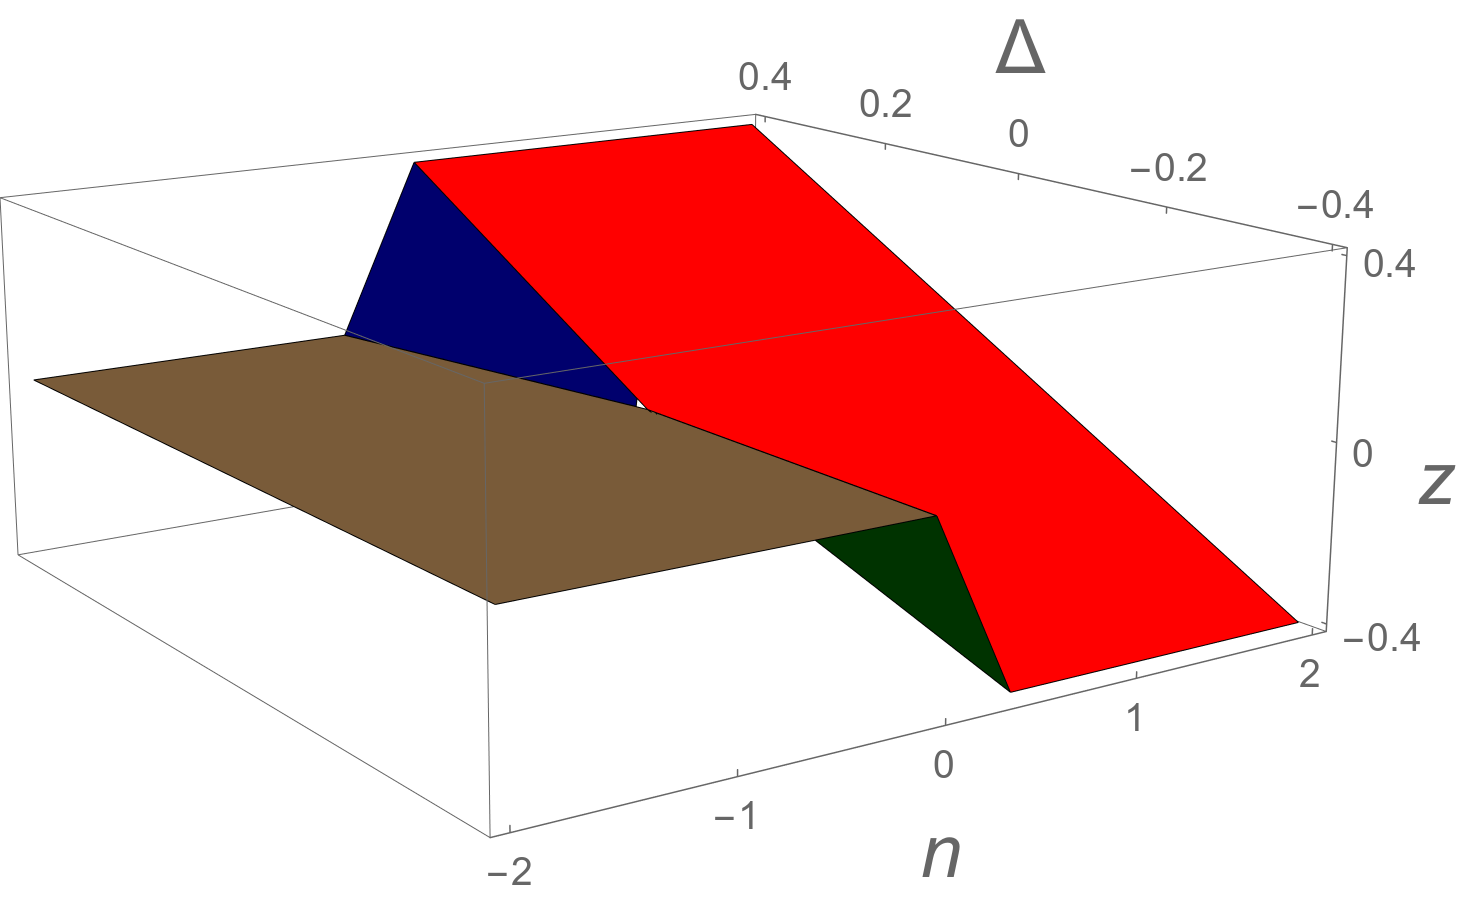
\includegraphics[width=\linewidth]{neurodiff/figs/equation1.png}
\caption{The shape of $ z = ReLU(n + \Delta) - ReLU(n) $.}
\label{neurodiff:fig:equation1}
\end{minipage}%
%
\hspace{0.09\linewidth}
%
\begin{minipage}[t]{0.45\linewidth}
\centering
%\captionsetup{width=0.98\textwidth}
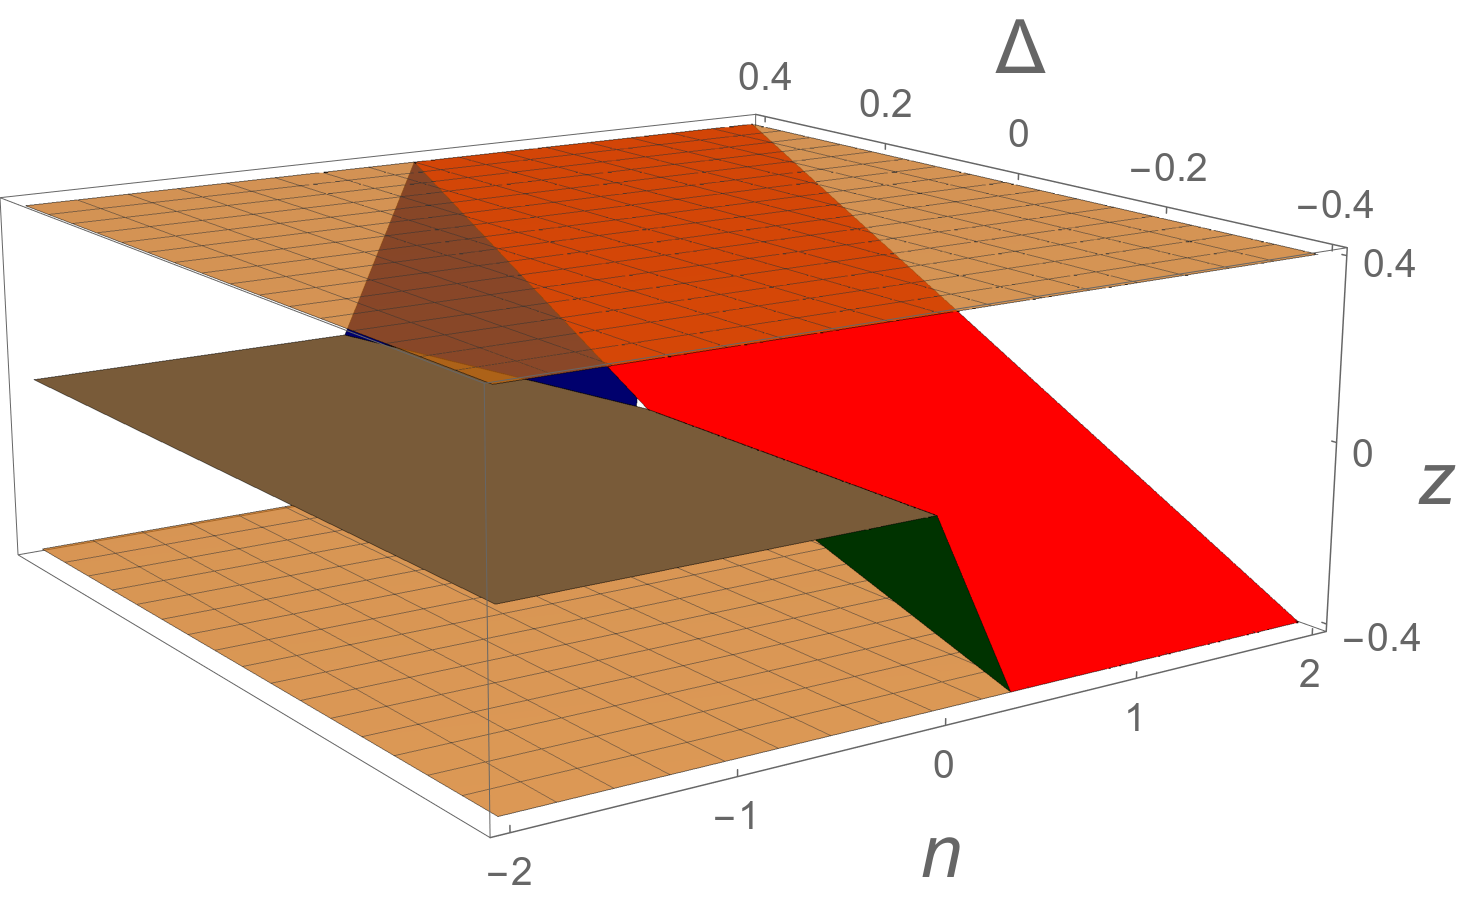
\includegraphics[width=\linewidth]{neurodiff/figs/naiveboundingplanes.png}
\caption{Bounding planes computed by \ReluDiff{}~\cite{paulsen2020reludiff}.}
\label{neurodiff:fig:naiveboundingplanes}
\end{minipage}

\begin{minipage}[t]{0.45\linewidth}
\centering
%\captionsetup{width=0.98\textwidth}
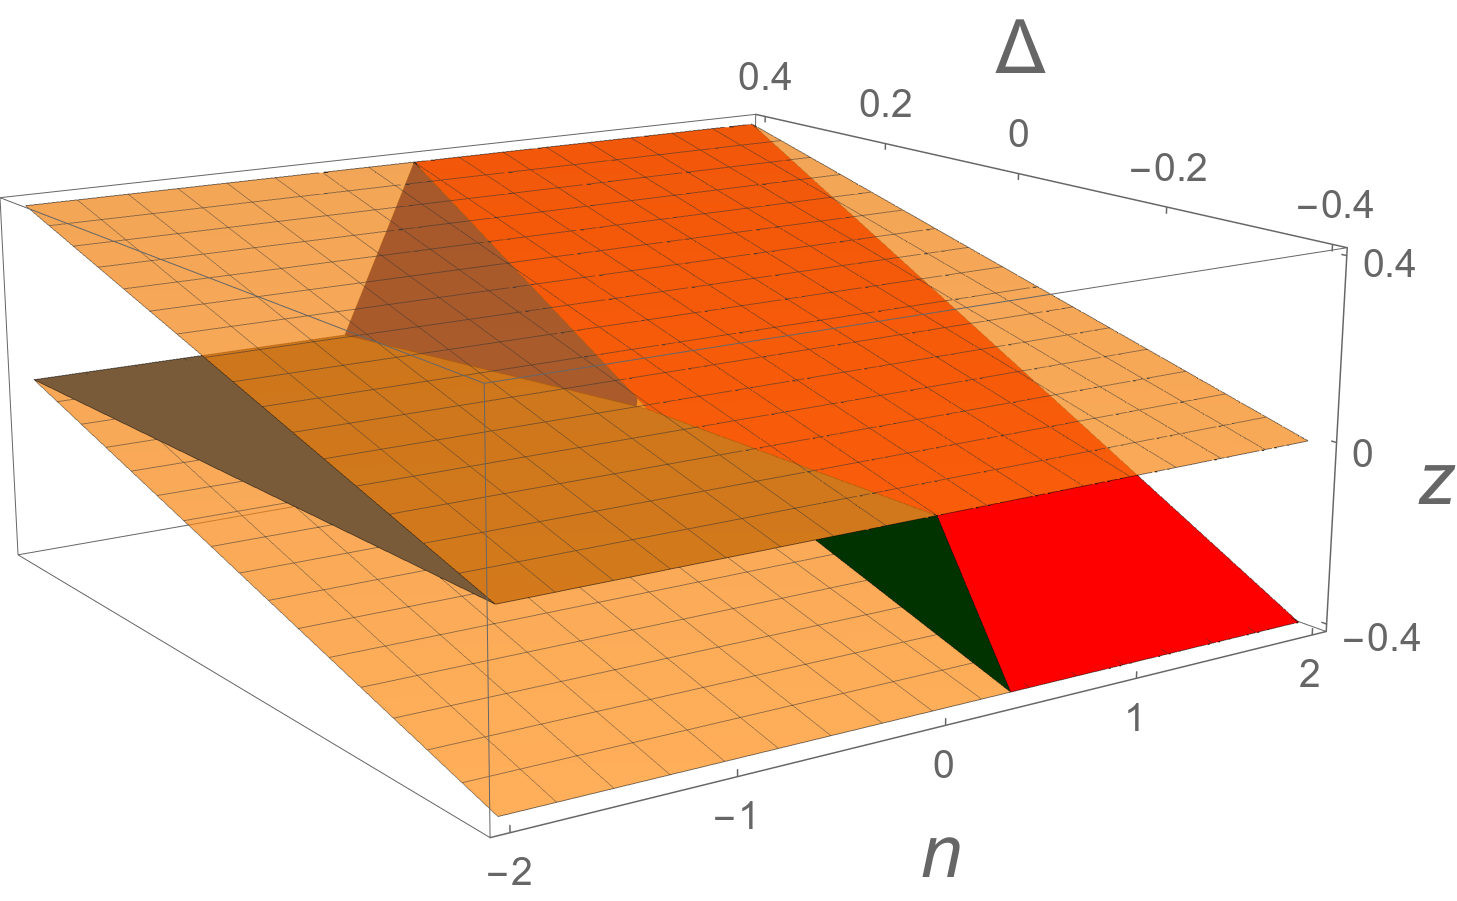
\includegraphics[width=\linewidth]{neurodiff/figs/linearboundingplanes.png}
\caption{Bounding planes computed by our new method.}
\label{neurodiff:fig:linearboundingplanes}
\end{minipage}%
%
\hspace{0.09\linewidth}
%
\begin{minipage}[t]{0.45\linewidth}
\centering
\scalebox{.65}{

\tikzset{every picture/.style={line width=0.75pt}} %set default line width to 0.75pt        

\begin{tikzpicture}[x=0.75pt,y=0.75pt,yscale=-1,xscale=1]
%uncomment if require: \path (0,300); %set diagram left start at 0, and has height of 300

%Straight Lines [id:da5621186100506654] 
\draw [color={rgb, 255:red, 199; green, 199; blue, 199 }  ,draw opacity=1 ]   (102,180) -- (338,180) ;
\draw [shift={(340,180)}, rotate = 180] [color={rgb, 255:red, 199; green, 199; blue, 199 }  ,draw opacity=1 ][line width=0.75]    (10.93,-3.29) .. controls (6.95,-1.4) and (3.31,-0.3) .. (0,0) .. controls (3.31,0.3) and (6.95,1.4) .. (10.93,3.29)   ;
\draw [shift={(100,180)}, rotate = 0] [color={rgb, 255:red, 199; green, 199; blue, 199 }  ,draw opacity=1 ][line width=0.75]    (10.93,-3.29) .. controls (6.95,-1.4) and (3.31,-0.3) .. (0,0) .. controls (3.31,0.3) and (6.95,1.4) .. (10.93,3.29)   ;
%Straight Lines [id:da9708804498380784] 
\draw [color={rgb, 255:red, 199; green, 199; blue, 199 }  ,draw opacity=1 ]   (220,62) -- (220,238) ;
\draw [shift={(220,240)}, rotate = 270] [color={rgb, 255:red, 199; green, 199; blue, 199 }  ,draw opacity=1 ][line width=0.75]    (10.93,-3.29) .. controls (6.95,-1.4) and (3.31,-0.3) .. (0,0) .. controls (3.31,0.3) and (6.95,1.4) .. (10.93,3.29)   ;
\draw [shift={(220,60)}, rotate = 90] [color={rgb, 255:red, 199; green, 199; blue, 199 }  ,draw opacity=1 ][line width=0.75]    (10.93,-3.29) .. controls (6.95,-1.4) and (3.31,-0.3) .. (0,0) .. controls (3.31,0.3) and (6.95,1.4) .. (10.93,3.29)   ;
%Straight Lines [id:da43894388755903013] 
\draw [color={rgb, 255:red, 74; green, 144; blue, 226 }  ,draw opacity=1 ][line width=1.5]    (220,180) -- (340,60) ;
%Straight Lines [id:da1261778605228432] 
\draw [color={rgb, 255:red, 74; green, 144; blue, 226 }  ,draw opacity=1 ][line width=1.5]    (220,180) -- (100,180) ;
%Straight Lines [id:da002818047409691604] 
\draw [color={rgb, 255:red, 0; green, 0; blue, 0 }  ,draw opacity=1 ] [dash pattern={on 4.5pt off 4.5pt}]  (320,80) -- (120,180) ;
%Straight Lines [id:da1715235527986837] 
\draw [color={rgb, 255:red, 0; green, 0; blue, 0 }  ,draw opacity=1 ] [dash pattern={on 4.5pt off 4.5pt}]  (320,130) -- (120,230) ;
%Straight Lines [id:da21391376020902975] 
\draw    (120,175.28) -- (120,180) ;
%Straight Lines [id:da9349071337756625] 
\draw    (120,180) -- (120,184.72) ;
%Straight Lines [id:da2699517570437805] 
\draw    (320,175.28) -- (320,180) ;
%Straight Lines [id:da4265291468096436] 
\draw    (320,180) -- (320,184.72) ;

% Text Node
\draw (117.5,196) node  [font=\Large]  {$\underline{LB}\left( n \right)$};
% Text Node
\draw (337,196) node  [font=\Large]  {$\overline{UB}\left( n \right)$};
% Text Node
\draw (166.5,140.5) node  [font=\Large,rotate=-333.19]  {$UB( ReLU(n) )$};
% Text Node
\draw (300,152.46) node  [font=\Large,rotate=-333.19]  {$LB( ReLU(n) )$};


\end{tikzpicture}
}
\caption{Bounding planes computed by \Neurify{}~\cite{WangPWYJ18nips}.}
\label{neurodiff:fig:wangconvex}
\end{minipage}
\end{figure*}


The key contribution in \Name{}, our new method, is a \emph{symbolic}
and \emph{fine-grained} approximation technique that both reduces the
approximation error introduced when a neuron is in an unstable state,
and mitigates the explosion of such approximation error after it is
introduced.


\subsubsection{Convex Approximation for the Difference Interval}

Our first contribution is developing convex approximations to directly
bound the difference between two neurons after these ReLU activations.
Specifically, for a neuron $ n $ in $ f $ and corresponding neuron $
n' $ in $ f' $, we want to bound the value of $ \relu{n'} - \relu{n}
$. We illustrate the various choices using
Figures~\ref{neurodiff:fig:equation1}, \ref{neurodiff:fig:naiveboundingplanes},
and~\ref{neurodiff:fig:linearboundingplanes}.


The naive way to bound this difference is to first compute
approximations of $ y = \relu{n} $ and $ y' = \relu{n'} $ separately,
and then subtract them.  Since each of these functions has a single
variable, convex approximation is simple and is already used by
single-network verification tools~\cite{SinghGPV19,WangPWYJ18nips,WengZCSHDBD18}.
Figure~\ref{neurodiff:fig:wangconvex} shows the function $y=\relu{n}$ and its
bounding planes (shown as dashed-lines) in a two-dimensional space (details in
Section~\ref{neurodiff:sec:preliminary}).
%
However, as we have already mentioned, approximation errors would be
accumulated in the bounds of $\relu{n}$ and $\relu{n'}$ and then amplified
by the interval subtraction.  This is precisely why the naive approach
performs poorly.


The \ReluDiff{} method of Paulsen et al.~\cite{paulsen2020reludiff} improves
upon the new approximation by computing an interval bound on $ n' - n
$, denoted $ \Delta $, then rewriting $z = \relu{n'} - \relu{n} $ as $
z= \relu{n + \Delta} - \relu{n} $, and finally bounding this new
function instead.
%
Figure~\ref{neurodiff:fig:equation1} shows the shape of $ z = \relu{n
+ \Delta}- \relu{n} $ in a three-dimensional space. Note that it has
four piece-wise linear subregions, defined by values of the input
variables $n$ and $\Delta$.
%
While the bounds computed by \ReluDiff{}~\cite{paulsen2020reludiff}, shown as
the (horizontal) yellow planes in
Figure~\ref{neurodiff:fig:naiveboundingplanes}, are sound, in practice they tend
to be loose because the upper and lower bounds are both concrete
values.  Such eager concretization eliminates symbolic information
that $ \Delta $ contained before applying the ReLU activation.


In contrast, our method computes a convex approximation of $ z $,
shown by the (tilted) yellow planes in
Figure~\ref{neurodiff:fig:linearboundingplanes}.
%
Since these tilted bounding planes are in a three-dimensional space,
they are significantly more challenging to compute than the standard
two-dimensional convex approximations (shown in
Figure~\ref{neurodiff:fig:wangconvex})
used by single network verification tools.
%convex approximation (shown in Figure~\ref{neurodiff:fig:wangconvex}) in a
%two-dimentionsl space, which was used by single-network verification
%tools.
%
Our approximations have the advantage of introducing significantly less
error than the horizontal planes used
in \ReluDiff{}~\cite{paulsen2020reludiff}, while maintaining some of the
symbolic information for $ \Delta $ before applying the ReLU
activation.


We will show through experimental evaluation
(Section~\ref{neurodiff:sec:experiment}) that our convex approximation can
drastically improve the accuracy of the difference bounds, and are
particularly effective when the input region being considered is
large.  Furthermore, the tilted planes shown in
Figure~\ref{neurodiff:fig:linearboundingplanes} are for the general case.  For
certain special cases, we obtain even tighter bounding planes (details
in Section~\ref{neurodiff:sec:approach}).
%
In the running example, using our new convex approximations would
improve the final bounds to $ [-1.97, 1.42] $.


\subsubsection{Symbolic Variables for Hidden Neurons}

Our second contribution is introducing symbolic variables to represent
the output values of some unstable neurons, with the goal of limiting
the propagation of approximation errors after they are introduced.
%
In the running example, since both $ \n{1}{1} $ and $ \np{1}{1} $ are in unstable states,
i.e., the input intervals of the ReLUs contain the value 0, we may introduce a
new
symbol $ x_3 = \relu{\np{1}{1}} - \relu{\n{1}{1}} $.  In all
subsequent layers, whenever the value of $\relu{\np{1}{1}}
- \relu{\n{1}{1}}$ is needed, we use the bounds $[x_3,x_3]$ instead of
the actual bounds.


The reason why using $x_3$ can lead to more accurate results is
because, even though our convex approximations reduce the error
introduced, there is inevitably some error that accumulates. Introducing $
x_3 $ allows this error to partially cancel in the subsequent
layers. In our running example, introducing the new symbolic variable
$x_3$ would be able to improve the final bounds to $ [-1.65, 1.18] $.


While creating $ x_3 $ improved the result
in this case, carelessly introducing new variables for all the unstable
neurons can actually reduce the overall benefit (see
Section~\ref{neurodiff:sec:approach}). In addition, the
computational cost of introducing new variables is not negligible.
%While substituting the values of unstable neurons with new symoblic
%variables may increases the accuracy of interval analysis, it may also
%add computational cost.
Therefore, in practice, we must introduce
these symbolic variables judiciously, to maximize the benefit.
%
Part of our contribution in \Name{} is in developing heuristics to
automatically determine when to create new symbolic variables (details
in Section~\ref{neurodiff:sec:approach}).



\section{Background}
\label{neurodiff:sec:preliminary}

In this section, we review the technical background and then introduce
notations that we use throughout the paper.

\subsection{Neural Networks}

% Define a neural network
% Limit ourselves to FFN ReLU networks
% Weight matrix notation
%	- W_k is the matrix for layer k
%	- W_k[i,j] is the weight of connection from n_k-1,i to n_k,j
We focus on feed-forward neural networks, which we define as a function $ f $ that takes
an $ n $-dimensional vector of real values $x \in \mathbb{X}$, where
$\mathbb{X} \subseteq \mathbb{R}^n $, and maps it to an $ m
$-dimensional vector $ y \in \mathbb{Y}$, where
$\mathbb{Y} \subseteq \mathbb{R}^m $.  We denote this function as $ f
: \mathbb{X} \to \mathbb{Y} $.  Typically, each dimension of $ y $
represents a score, such as a probability, that the input $ x $
belongs to class $ i $, where $ 1 \leq i \leq m $.

A network with $l$ layers has $ l $ weight matrices, each of which is
denoted $ \Wk{k}, $ for $ 1 \leq k \leq l $. For each weight matrix, we
have $ \Wk{k} \in \mathbb{R}^{l_{k-1} \times l_k} $ where $ l_{k-1} $
is the number of neurons in layer $ (k-1) $ and likewise for $ l_k $,
and $ l_0 = n $.
Each element in $ \Wk{k} $ represents the weight of an edge from a
neuron in layer $ (k-1) $ to one in layer $ k $. Let $ \n{k}{j} $
denote the $ j^{th} $ neuron of layer $ k $, and $ \n{k-1}{i} $ denote
the $ i^{th} $ neuron of layer $ (k-1) $.  We use $ \W{k}{i}{j} $ to
denote the edge weight from $ \n{k-1}{i} $ to $ \n{k}{j} $.
%
In our motivating example, we have $ W_1[1,1] = 1.9 $ and $ W_1[1,2] =
1.1 $.

Mathematically, the entire neural network can be represented by $ f(x)
= f_l(\, W_l \cdot \, f_{l-1}( \, W_{l-1} \, \cdot ...f_1(W_1 \cdot
x)...)) $, where $ f_k $ is the activation function of the $
k^{th} $ layer and $1\leq k\leq l$. We focus on neural networks with
ReLU activations because they are the most widely implemented in
practice, but our method can be extended to other activation
functions, such as $sigmoid$ and $tanh$, and other layer types, such
as convolutional and max-pooling. We leave this as future work.

\subsection{Symbolic Intervals}

% Introduce notation for intervals
To compute approximations of the output nodes that are sound for all
input values, we leverage interval
arithmetic~\cite{moore2009introduction}, which can be viewed as an
instance of the abstract interpretation framework~\cite{CousotC77}. It
is well-suited to the verification task because interval arithmetic is
soundly defined for basic operations of the network such as addition,
subtraction, and scaling.

Let $ I = [\LBEq{I}, \UBEq{I}] $ be an interval with lower bound
$ \LBEq{I} $ and upper bound $ \UBEq{I} $. Then, for intervals $ I_1,
I_2 $, we have addition and subtraction defined as $ I_1 + I_2 =
[\LBEq{I_1} + \LBEq{I_2}, \UBEq{I_1} + \UBEq{I_2}] $ and $ I_1 - I_2 =
[\LBEq{I_1} - \UBEq{I_2}, \UBEq{I_1} - \LBEq{I_2}] $, respectively.
For a constant $ c $, scaling is defined as $ c \times I_1 =
[c \times \LBEq{I_1}, c \times \UBEq{I_1} $ when $ c > 0 $, and $
c \times I_1 = [c \times \UBEq{I_1}, c \times \LBEq{I_1}] $ otherwise.

While interval arithmetic is a sound over-approximation, it is not
always accurate.  To illustrate, let $ f(x) = 3x - x $, and say we are
interested in bounding $ f(x) $ when $ x \in [-1, 1] $. One way to
bound $ f $ is by evaluating $ f(I) $ where $ I = [-1, 1] $. Doing so
yields $ 3 \times [-1, 1] - [-1, 1] = [-4, 4] $. Unfortunately, the most
accurate bounds are $ [-2, 2] $.


There are (at least) two ways we can improve the accuracy. First, we can
soundly refine the result by dividing the input intervals into disjoint
partitions, performing the analysis independently on each partition, and then
unioning the resulting output intervals together. Previous work has shown the
result will be \textit{at least} as precise~\cite{WangPWYJ18}, and often
better. For example, if we partition $ x \in [-1, 1] $ into $x\in[-1,0]$ and
$x\in[0,1]$, and perform the analysis for each partition, the
resulting bounds improve to $ [-3, 3] $.

% Introduce symblic interval concept and notation
Second, the dependence between the two intervals are
not leveraged when we subtract them, i.e., that they were both $ x $
terms and hence could partially cancel out.
To capture the dependence, we can use \textit{symbolic} lower and
upper bounds~\cite{WangPWYJ18}, which are expressions in
terms of the input variable, i.e., $ I = [x, x] $.  Evaluating $ f(I)
$ then yields the interval $ I_f = [2x, 2x] $, for $x\in[-1,1]$.  When using
symbolic bounds, eventually, we must concretize the lower and upper
bound equations. We denote concretization of $\LBEq{I_f}=2x$ and
$\UBEq{I_f}=2x$ as $ \LBL{I_f} = -2 $ and $ \UBU{I_f} = 2 $,
respectively.  Compared to the naive solution, $[-4,4]$, this is a
significant improvement.

When approximating the output of a given function $ f
: \mathbb{X} \to \mathbb{Y} $ over an input interval $
X \subseteq \mathbb{X} $, one may prove soundness by showing that the
evaluation of the lower and upper bounds on any input $ x \in X $ are
always greater than and less than, respectively, to the true value of
$ f(x) $.
%
Formally, for an interval $ I $, let $ \LBEq{I}(x) $ be the evaluation
of the lower bound equation on input $ x $, and similarly for
$ \UBEq{I}(x) $. Then, the approximation is considered sound if
$ \forall x \in X$, we have $\LBEq{I}(x) \leq f(x) \leq \UBEq{I}(x) $.

\subsection{Convex Approximations}
While symbolic intervals are exact for linear operations
(i.e. they do not introduce error), this is not the case
for non-linear operations, such as the ReLU activation.
%While using symbolic intervals in linear operations can avoid
%approximation errors, this is no longer possible for non-linear
%operations such as ReLU activation.
This is because, for efficiency
reasons, the symbolic lower and upper bounds must be kept linear.
Thus, developing linear approximations for non-linear activation
functions has become a signifciant area of research for single neural
network
verification~\cite{WangPWYJ18nips,SinghGPV19,WengZCSHDBD18,zhang2018efficient}. We
review the basics below, but caution that they are different from our
new convex approximations in \Name{}.

We denote the input to the ReLU of a neuron $ \nj $ as $ \IntIn{\nj} $
and the output as $ \IntOut{\nj} $. The approach used by existing
single-network verification tools is to apply an affine transformation
to the upper bound of $ \IntIn{\nj} $ such that
$ \UBEq{\IntIn{\nj}}(x) \geq 0 $, where $ x \in X $, and $ X $ is the
input region for the entire network.  For the lower bound, there exist
several possible transformations, including the one used
by \Neurify{}~\cite{WangPWYJ18nips}, shown in
Figure~\ref{neurodiff:fig:wangconvex}, where $n = \IntIn{\nj}$ and the dashed
lines are the upper and lower bounds.

We illustrate the upper bound transformation for $ \n{1}{1} $ of our
motivating example. After computing the upper bound of the ReLU
input $ \UBEq{\IntIn{\n{1}{1}}} = 1.9x_1 - 1.9x_2 $, where
$x_1\in[-2,2]$ and $x_2\in[-2,2]$, it computes the concrete lower and
upper bounds. We denote these as $ \UBL{\IntIn{\n{1}{1}}} = -7.6 $
and $ \UBU{\IntIn{\n{1}{1}}} = 7.6 $. We refer to them as $ l $ and $
u $, respectively, for short hand. Then, it computes the line that
passes through $ (u, u) $ and $ (0, l) $.
%
Letting $ y = \UBEq{\IntIn{\n{1}{1}}} $ be the upper bound equation of the ReLU
input, it computes the upper bound of the ReLU output as
$ \UBEq{\IntOut{\n{1}{1}}} $ $ = \frac{u}{u - l}(y - l) = $ $ 0.95x_1
-0.95x_2 +3.81 $.

When considering a single ReLU of a single network, convex
approximation is simple because there are only three states that the
neuron can be in, namely active, inactive, and unstable. Furthermore,
in only one of these states, convex approximation is needed.
%
In contrast, differential verification has to consider a pair of
neurons, which has up to nine states to consider between the two
ReLUs.  Furthermore, different states may result in different linear
approximations, and some states can even have multiple linear
approximations depending on the difference bound of $ \Delta = n' - n
$. As we will show in Section~\ref{neurodiff:sec:approach}, there are
significantly more considerations in our problem domain.

\ignore{
\subsection{Refinement}
% Interval analysis
Often times, the output interval will not be tight enough to verify the desired property. One way to improve the result is to divide the input interval into disjoint sub-intervals, perform the analysis on each region, and then union the output intervals together. The resulting output interval is guaranteed to be at least as tight the original output interval~\cite{moore2009introduction}. In fact, previous work showed that, for ReLU networks, the analysis result can be made arbitrarily accurate through input partitioning based refinement~\cite{WangPWYJ18}.

The key challenge in this type of refinement is deciding how to partition the
input interval. Previous work~\cite{paulsen2020reludiff, WangPWYJ18,
WangPWYJ18nips} has seen success by computing \textit{smear
values}~\cite{kearfott1990algorithm, kearfott2013rigorous} for each input.
Informally, the smear value is a measure of how much influence a single input
neuron has on the output values.

For example, ....
}



\section{Our Approach}
\label{neurodiff:sec:approach}

We first present our baseline procedure for differential verification
of feed-forward neural networks (Section~\ref{neurodiff:sec:baseline}), and then
present our algorithms for computing convex approximations
(Section~\ref{neurodiff:sec:convex}) and introducing symbolic variables
(Section~\ref{neurodiff:sec:symbolic}).


\subsection{Differential Verification -- Baseline}
\label{neurodiff:sec:baseline}

We build off the work of Paulsen et al.~\cite{paulsen2020reludiff}, so in this
section
we review the relevant pieces. We assume that the input
to \Name{} consists of two networks $ f $ and $ f' $, each with $ l $ layers
of the same size.  Let $ \npj $ in $ f' $ be the neuron paired with
$ \nj $ in $ f $. This implicitly creates a pairing of the edge
weights between the two networks. We first introduce additional notation.
%
\begin{itemize}
\item
We denote the difference between a pair of neurons as $ \ndj = \npj
- \nj $. For example, $ \nd{1}{1} = 0.1 $ under the input $ x_1 = 2, x_2 =
1 $ in our motivating example shown in Figure~\ref{neurodiff:fig:motex}.
\item
We denote the difference in a pair of edge weights as $ \Wd{k}{i}{j}
= \Wp{k}{i}{j} - \W{k}{i}{j} $. For example, $ \Wd{1}{1}{1} = 2.0 -
1.9 = 0.1 $.
\item
We extend the symbolic interval notation to these terms. That is,
$ \IntIn{\ndj} $ denotes the interval that bounds $ \npj - \nj $
before applying ReLU, and $ \IntOut{\ndj} $ denotes the interval after
applying ReLU.
\end{itemize}

Given that we have computed $ \IntOut{\n{k-1}{i}}$,
$\IntOut{\np{k-1}{i}}$, $\IntOut{\nd{k-1}{i}} $ for every neuron in
the layer $ k - 1 $, now, we compute a single $ \IntOut{\nd{k}{j}} $
in the subsequent layer $k$ in two steps (and then repeat for each $ 1 \leq
j \leq l_k $).

%\begin{enumerate}
%\item
First, we compute $ \IntIn{\nd{k}{j}} $ by propagating the output
intervals from the previous layer through the edges connecting to the
target neuron. This is defined as
%
\[
	\IntIn{\nd{k}{j}} = \sum_{i} \bigg( \IntOut{\nd{k-1}{i}} \times \Wp{k}{i}{j} + \IntOut{\n{k-1}{i}} \times \Wd{k-1}{i}{j} \bigg)
\]
%
We illustrate this computation on node $ \nd{1}{1} $ in our
example. First, we initialize $ \IntOut{\nd{0}{1}} $  $ = $  $ [0,0] $ ,
$\IntOut{\nd{0}{2}} = [0,0]$. Then we compute $ \IntIn{\nd{1}{1}} $  $ =
[0, 0] \times 2.0 +$$ [x_1, x_1] \times 0.1 + $$ [0, 0] \times -2.0 +
$ $ [x_2, x_2] \times -0.1 = $ $[0.1x_1 - 0.1x_2,$ $ 0.1x_1 - 0.1x_2]
$.

%\item
For the second step, we apply ReLU to $ \IntIn{\nd{k}{j}} $ to obtain
$ \IntOut{\nd{k}{j}} $. This is where we apply the new convex
approximations (Section~\ref{neurodiff:sec:convex}) to obtain tighter bounds.
Toward this end, we will focus on the following two equations:
%
\begin{align}
z_1 = \relu{{\nj} + {\ndj}} - \relu{{\nj}} \label{neurodiff:eq:1}\\
z_2 = \relu{{\npj}} - \relu{{\npj} - {\ndj}} \label{neurodiff:eq:2}
\end{align}
%
While Paulsen et al.~\cite{paulsen2020reludiff} also compute bounds of these
two equations, they use \emph{concretizations} instead of \emph{linear
approximations}, thus throwing away all the symbolic information.  For
the running example, their method would result in the bounds of
$ \IntOut{\nd{1}{1}} = [-.4, .4] $. In contrast, our method will be
able to maintain some or all of the symbolic information, thus
improving the accuracy.
%\end{enumerate}




\subsection{Two Useful Lemmas}

\begin{figure}[t]
	\centering
	\scalebox{1.0}{

\tikzset{every picture/.style={line width=0.75pt}} %set default line width to 0.75pt        

\begin{tikzpicture}[x=0.75pt,y=0.75pt,yscale=-1,xscale=1]
%uncomment if require: \path (0,300); %set diagram left start at 0, and has height of 300

%Straight Lines [id:da5621186100506654] 
\draw [color={rgb, 255:red, 0; green, 0; blue, 0 }  ,draw opacity=1 ][fill={rgb, 255:red, 0; green, 0; blue, 0 }  ,fill opacity=1 ]   (102,180) -- (338,180) ;
\draw [shift={(340,180)}, rotate = 180] [color={rgb, 255:red, 0; green, 0; blue, 0 }  ,draw opacity=1 ][line width=0.75]    (10.93,-3.29) .. controls (6.95,-1.4) and (3.31,-0.3) .. (0,0) .. controls (3.31,0.3) and (6.95,1.4) .. (10.93,3.29)   ;
\draw [shift={(100,180)}, rotate = 0] [color={rgb, 255:red, 0; green, 0; blue, 0 }  ,draw opacity=1 ][line width=0.75]    (10.93,-3.29) .. controls (6.95,-1.4) and (3.31,-0.3) .. (0,0) .. controls (3.31,0.3) and (6.95,1.4) .. (10.93,3.29)   ;
%Straight Lines [id:da9708804498380784] 
\draw [color={rgb, 255:red, 0; green, 0; blue, 0 }  ,draw opacity=1 ][fill={rgb, 255:red, 0; green, 0; blue, 0 }  ,fill opacity=1 ]   (220,92) -- (220,268) ;
\draw [shift={(220,270)}, rotate = 270] [color={rgb, 255:red, 0; green, 0; blue, 0 }  ,draw opacity=1 ][line width=0.75]    (10.93,-3.29) .. controls (6.95,-1.4) and (3.31,-0.3) .. (0,0) .. controls (3.31,0.3) and (6.95,1.4) .. (10.93,3.29)   ;
\draw [shift={(220,90)}, rotate = 90] [color={rgb, 255:red, 0; green, 0; blue, 0 }  ,draw opacity=1 ][line width=0.75]    (10.93,-3.29) .. controls (6.95,-1.4) and (3.31,-0.3) .. (0,0) .. controls (3.31,0.3) and (6.95,1.4) .. (10.93,3.29)   ;
%Straight Lines [id:da43894388755903013] 
\draw [color={rgb, 255:red, 74; green, 144; blue, 226 }  ,draw opacity=1 ][line width=1.5]    (140,260) -- (300,100) ;
%Straight Lines [id:da002818047409691604] 
\draw [color={rgb, 255:red, 0; green, 0; blue, 0 }  ,draw opacity=1 ] [dash pattern={on 4.5pt off 4.5pt}]  (300,100) -- (140,200) ;
%Straight Lines [id:da1715235527986837] 
\draw [color={rgb, 255:red, 0; green, 0; blue, 0 }  ,draw opacity=1 ] [dash pattern={on 4.5pt off 4.5pt}]  (300,160) -- (140,260) ;
%Straight Lines [id:da5537839721735281] 
\draw    (140,174) -- (140,186) ;
%Straight Lines [id:da6486767585115278] 
\draw    (300,174) -- (300,186) ;

% Text Node
\draw (136,125.4) node [anchor=north west][inner sep=0.75pt]    {$( x-l)\frac{u-l'}{u-l} +l'$};
% Text Node
\draw (223,207.4) node [anchor=north west][inner sep=0.75pt]    {$( x-u)\frac{u'-l}{u-l} +u'$};
% Text Node
\draw (137,160.4) node [anchor=north west][inner sep=0.75pt]    {$l$};
% Text Node
\draw (296,187.4) node [anchor=north west][inner sep=0.75pt]    {$u$};


\end{tikzpicture}
}
	\caption{Illustration of Lemmas~\ref{neurodiff:lemma:1}
	and~\ref{neurodiff:lemma:2}.\label{neurodiff:fig:lemma_fig}}
\end{figure}

Before presenting our new linear approximations, we introduce two
useful lemmas, which will simplify our presentation as well as our
soundness proofs.

\begin{lemma}\label{neurodiff:lemma:1}
	Let $ x $ be a variable such that $ l \leq x \leq u $ for constants $ l \leq 0 $ and $ 0 \leq u $. For a constant $ l' $ such that $ l \leq l' \leq 0 $, we have $ x \leq (x - l) * \frac{u - l'}{u - l} + l' \geq l' $.
\end{lemma}
\begin{lemma}\label{neurodiff:lemma:2}
	Let $ x $ be a variable such that $ l \leq x \leq u $ for constants $ l \leq 0 $ and $ 0 \leq u $. For a constant $ u' $ such that $ 0 \leq u' \leq u $, we have $ u' \geq (x - u) * \frac{u' - l}{u - l} + u' \leq x $.
\end{lemma}

We illustrate these lemmas in Figure~\ref{neurodiff:fig:lemma_fig}. The solid
blue line shows the equation $ y = x $ for the input interval $ l \leq
x \leq u $. The upper dashed line illustrates the transformation of
Lemma~\ref{neurodiff:lemma:1}, and the lower dashed line illustrates
Lemma~\ref{neurodiff:lemma:2}. Specifically, Lemma~\ref{neurodiff:lemma:1} shows a
transformation applied to $ x $ whose result is always greater than
both $ l' $ and $ x $. Similarly, Lemma~\ref{neurodiff:lemma:2} shows a
transformation applied to $ x $ whose result is always less than both
$ u' $ and $ x $. These lemmas will be useful in bounding
Equations~\ref{neurodiff:eq:1}
and~\ref{neurodiff:eq:2}.

\subsection{New Convex Approximations for $ \IntOut{\ndj} $}
\label{neurodiff:sec:convex}

Now, we are ready to present our new approximations, which are
linear symbolic expressions derived from Equations~\ref{neurodiff:eq:1}
and~\ref{neurodiff:eq:2}.


We first assume that $ \nj $ and $ \npj $ could both be unstable,
i.e., they could take values both greater than and less than 0. This
yields bounds for the general case in that they are sound in all
states of $ \nj $ and $ \npj $ (Sections~\ref{neurodiff:sec:upper}
and \ref{neurodiff:sec:lower}).
%
Then, we consider special cases of $ \nj $ and $ \npj $, in
which even tighter upper and lower bounds are derived
(Section~\ref{neurodiff:sec:tighter}).

\declarecommand{\nn}[0]{n}
\declarecommand{\nnp}[0]{n'}
\declarecommand{\nnd}[0]{\Delta}

To simplify notation, we let $ \nn, \nnp,$ and $ \nnd $ stand in for $ \nj,
\npj, $ and $ \ndj $ in the remainder of this section.

\subsubsection{Upper Bound for the General Case}
\label{neurodiff:sec:upper}

Let $ l = \UBL{\IntIn{\nnd}}$ and $ u = \UBU{\IntIn{\nnd}} $. The
upper bound approximation is:
%
\[
\UBEq{\IntOut{\nnd}} = \begin{cases}
\UBEq{\IntIn{\nnd}} & \UBL{\IntIn{\nnd}} \geq 0\\
0 & \UBU{\IntIn{\nnd}} \leq 0 \\
(\UBEq{\IntIn{\nnd}} - l)*\frac{u}{u - l} & otherwise
\end{cases}
\]
%
That is, when the input's (delta) upper bound is greater than 0 for all $
x \in X $, we can use the input's upper bound unchanged.  When the
upper bound is always less than 0, the new output's upper
bound is then 0. Otherwise, we apply a linear transformation to the
upper bound, which results in the upper plane illustrated in
Figure~\ref{neurodiff:fig:linearboundingplanes}. We prove all three cases sound.

\begin{proof}

We consider each case above separately. In the following, we use
Equation~\ref{neurodiff:eq:1} to derive the bounds, but we note a symmetric proof
using
Equation~\ref{neurodiff:eq:2} exists and produces the same bounds.

\paragraph{Case 1: $ \UBL{\IntIn{\nnd}} \geq 0 $.}
We first show that, according to Equation~\ref{neurodiff:eq:1}, when $ 0 \leq
\nnd $ we have $ z_1 \leq \nnd $. This then implies that, if
$ \UBL{\IntIn{\nnd}} \geq 0 $, then $ z_1 \leq \UBEq{\IntIn{\nnd}}(x)
$ for all $ x \in X $, and hence it is a valid upper bound for the output
interval.

Assume $ 0 \leq \nnd $. We consider two cases of $ \nn $. First, consider
$ 0 \leq \nn $. Observe $ 0 \leq \nn \wedge 0 \leq \nnd $ $ \implies $
$ 0 \leq \nn + \nnd $. Thus, the ReLU's of Equation~\ref{neurodiff:eq:1}
simplify to $ z_1 = \nn + \nnd - \nn = \nnd \implies z_1 \leq \nnd
$. When $ \nn < 0 $, Equation~\ref{neurodiff:eq:1} simplifies to $ z_1
= \relu{\nn + \nnd} $. Since $ \nn < 0 $, we have $ \nn
+ \nnd \leq \nnd \wedge 0 \leq \Delta $ $ \implies $ $ \relu{\nn + \nnd}
\leq \nnd$. Thus,
$ z_1 = \relu{\nn + \nnd} \leq \nnd $, so the approximation is
sound.

\paragraph{Case 2: $ \UBU{\IntIn{\nnd}} \leq 0 $.}
This case was previously proven~\cite{paulsen2020reludiff}, but we restate it
here.  $ \UBU{\IntIn{\nnd}} \leq 0 $ $ \iff $ $ \nnp \leq \nn $ $ \implies $
$\relu{\nnp} \leq \relu{\nn} $
$ \iff $ $ \relu{\nnp} - \relu{\nn} \leq 0 $.

\paragraph{Case 3.}
By case 1, any $ \UBEq{\IntOut{\nnd}} $ that satisfies
$ \UBEq{\IntOut{\nnd}}(x) $ $ \geq 0 $ and $ \UBEq{\IntOut{\nnd}}(x) \geq
$ $ \UBEq{\IntIn{\nnd}}(x) $ for all $ x \in X $ is sound. Both
inequalities hold by Lemma~\ref{neurodiff:lemma:1}, with $ x
= \UBEq{\IntIn{\nnd}} $, $l=\UBL{\IntIn{\nnd}}$,
$u=\UBU{\IntIn{\nnd}}$ and $ l' = 0 $.

\end{proof}


We illustrate the upper bound computation on node $ \n{1}{1} $ of our
motivating example. Recall that $ \UBEq{\IntIn{\n{1}{1}}} = 0.1x_1 -
0.1x_2 $. Since $ \UBL{\IntIn{\n{1}{1}}} = -0.4 $ and
$ \UBU{\IntIn{\n{1}{1}}} = 0.4 $, we are in the third case of our
linear approximation above. Thus, we have $ \UBEq{\IntIn{\n{1}{1}}}
= $$ ( 0.1x_1 - 0.1x_2 - (-0.4))*\frac{0.4}{0.4 - (-0.4)} = $$ 0.5x_1
- 0.5x_2 + 0.2 $. This is the upper bounding plane illustrated in
Figure~\ref{neurodiff:fig:linearboundingplanes}. The volume under this plane is
50\% less
than the upper bounding plane of \ReluDiff{} shown in
Figure~\ref{neurodiff:fig:naiveboundingplanes}.



\subsubsection{Lower Bound for the General Case}
\label{neurodiff:sec:lower}

Let $ l = \LBL{\IntIn{\nnd}} $ and $ u = $ $ \LBU{\IntIn{\nnd}} $, the
lower bound approximation  is:
\[
\LBEq{\IntOut{\nnd}} = \begin{cases}
\LBEq{\IntIn{\nnd}} 	& 		\LBU{\IntIn{\nnd}} \leq 0\\
0 				& 		\LBL{\IntIn{\nnd}} \geq 0 \\
(\LBEq{\IntIn{\nnd}} - u)*\frac{-l}{u - l} & otherwise
\end{cases}
\]
That is, when the input lower bound is always less than 0, we can
leave it unchanged. When it is always greater than 0, the new lower
bound is then 0.  Otherwise, we apply a transformation to the lower
bound, which results in the lower plane illustrated in
Figure~\ref{neurodiff:fig:linearboundingplanes}. We prove all three cases sound.


\begin{proof}
We consider each case above separately. In the following, we use
Equation~\ref{neurodiff:eq:1} to derive the bounds, but we note a symmetric proof
using
Equation~\ref{neurodiff:eq:2} exists and produces the same bounds.

\paragraph{Case 1: $ \LBU{\IntIn{\nnd}} \leq 0 $.}
We first show that according to Equation~\ref{neurodiff:eq:1}, when $ \nnd \leq 0
$ we
have $ \nnd \leq z_1 $. This then implies that, if $ \LBU{\IntIn{\nnd}} \leq 0
$, we have $ \LBEq{\IntIn{\nnd}}(x) \leq z_1 $ for all $ x \in X $, and hence
it is a valid lower bound for the output interval.

Assume $ \nnd \leq 0 $. We consider two cases of $ \nn + \nnd
$. First, let $ 0 \leq $ $ \nn + \nnd $. Observe $ 0 \leq $ $ \nn
+ \nnd \wedge \nnd \leq 0 $ $ \implies $ $ 0 \leq \nn $, so we can
simplify Equation~\ref{neurodiff:eq:1} to $ z_1 = \nn + \nnd - \nn
= \nnd \implies \nnd \leq z_1 $. Second, let $ \nn + \nnd <
0 \iff \nnd < -\nn $. Then, Equation~\ref{neurodiff:eq:1} simplifies to $ z_1 =
- \relu{\nn} = -max(0,\nn) = min(0, -\nn) $. Now observe $ \nnd <
-\nn \wedge \nnd < 0 \implies \nnd < min(0, -\nn) = z_1 $.

\paragraph{Case 2: $ \LBL{\IntIn{\nnd}} \geq 0 $.}
This case was previously proven sound \cite{paulsen2020reludiff}, but we
restate it here.
\\
$ \LBL{\IntIn{\nnd}} $  $ \geq 0 $ $ \iff $ $ \nnp \geq \nn $ $
\implies $ $ \relu{\nnp} \geq \relu{\nn} $ $ \iff $ $ \relu{\nnp} - \relu{\nn}
\geq 0 $.

\paragraph{Case 3.}
By case 1, any $ \LBEq{\IntOut{\nnd}} $ that satisfies
$ \LBEq{\IntOut{\nnd}}(x) \leq 0 $ and $ \LBEq{\IntOut{\nnd}}(x) $
$ \leq $ $ \LBEq{\IntIn{\nnd}}(x) $ for all $ x \in X $ will be valid. Both
inequalities hold by Lemma~\ref{neurodiff:lemma:2}, with $ x =
\LBEq{\IntIn{\nnd}}, u'
= 0, l = \LBL{\IntIn{\nnd}}, $ and $ u = \LBU{\IntIn{\nnd}} $.

\end{proof}


We illustrate the lower bound computation on node $ \n{1}{1} $ of our
motivating example. Recall that $ \LBEq{\IntIn{\n{1}{1}}} = 0.1x_1 -
0.1x_2 $. Since $ \LBL{\IntIn{\n{1}{1}}} = -0.4 $ and
$ \LBU{\IntIn{\n{1}{1}}} = 0.4 $, we are in the third case of our
linear approximation. Thus, we have $ \LBEq{\IntOut{\n{1}{1}}} = $ $
(0.1x_1 - 0.1x_2 - (-0.4))*\frac{-(-0.4)}{0.4 - (-0.4)} $$ = 0.05x_1 -
0.05x_2 - 0.2$. This is the lower bounding plane illustrated in
Figure~\ref{neurodiff:fig:linearboundingplanes}. The volume above this plane is
50\% less
than the lower bounding plane of \ReluDiff{} shown in
Figure~\ref{neurodiff:fig:naiveboundingplanes}.


\subsubsection{Tighter Bounds for Special Cases}
\label{neurodiff:sec:tighter}

While the bounds presented so far apply in all states of $ \nn $ and
$ \nnp $, under certain conditions, we are able to tighten these
bounds even further.
%
Toward this end, we restate the following two lemmas proved by Paulsen
et al.~\cite{paulsen2020reludiff}, which will come in handy.  They are related
to properties of Equations~\ref{neurodiff:eq:1} and \ref{neurodiff:eq:2},
respectively.
%
\begin{lemma} \label{neurodiff:lemma:prev1}
	$ \relu{{\nn} + {\nnd}} - \nn \equiv max(-\nn, \nnd)$
\end{lemma}
\begin{lemma} \label{neurodiff:lemma:prev2}
	$ \nnp - \relu{{\nnp} - {\nnd}} \equiv min(\nnp, \nnd)$
\end{lemma}
%
These lemmas provide bounds when $ \nn $ and $ \nnp $ are proved to be
linear based on the absolute bounds that we compute.

\paragraph{Tighter Upper Bound When $ \nnp $ Is Linear.}

In this case, we have $ \UBEq{\IntOut{\nnd}} $ $ = $
$ \UBEq{\IntIn{\nnd}}$, which is an improvement for the second or
third case of our general upper bound.

\begin{proof}
By our case assumption, Equation~\ref{neurodiff:eq:2} simplifies to the one in
Lemma~\ref{neurodiff:lemma:prev2}. Thus, $ z_2 =$ $ min(\nnp, \nnd) $ $\implies
z_2 \leq \nnd $.
\end{proof}

\begin{figure*}
	\centering
	%
	\begin{minipage}[t]{0.45\linewidth}
		\centering
		%\captionsetup{width=0.98\textwidth}
		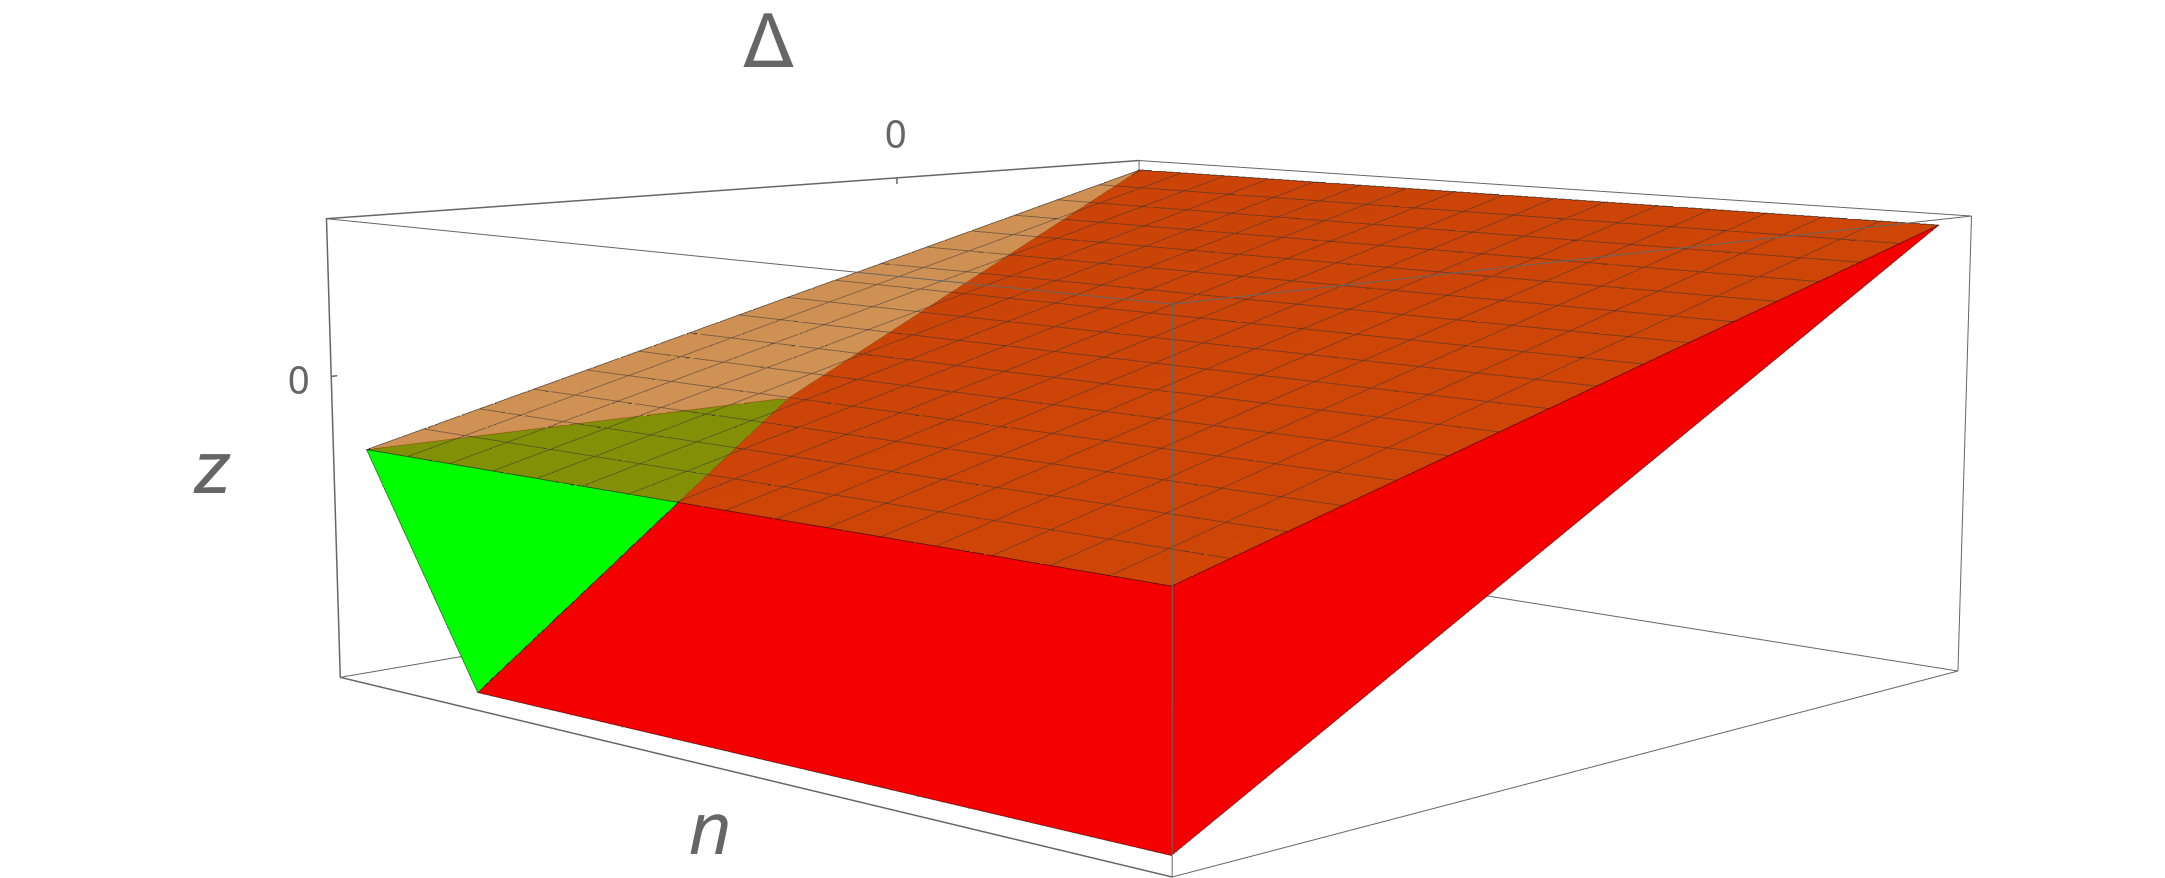
\includegraphics[width=\linewidth]{neurodiff/figs/specialcase1.png}
		\caption{Tighter upper bounding plane.}
		\label{neurodiff:fig:specialcase1}
	\end{minipage}%
	%
	\hspace{0.09\linewidth}
	%
	\begin{minipage}[t]{0.45\linewidth}
		\centering
		%\captionsetup{width=0.98\textwidth}
		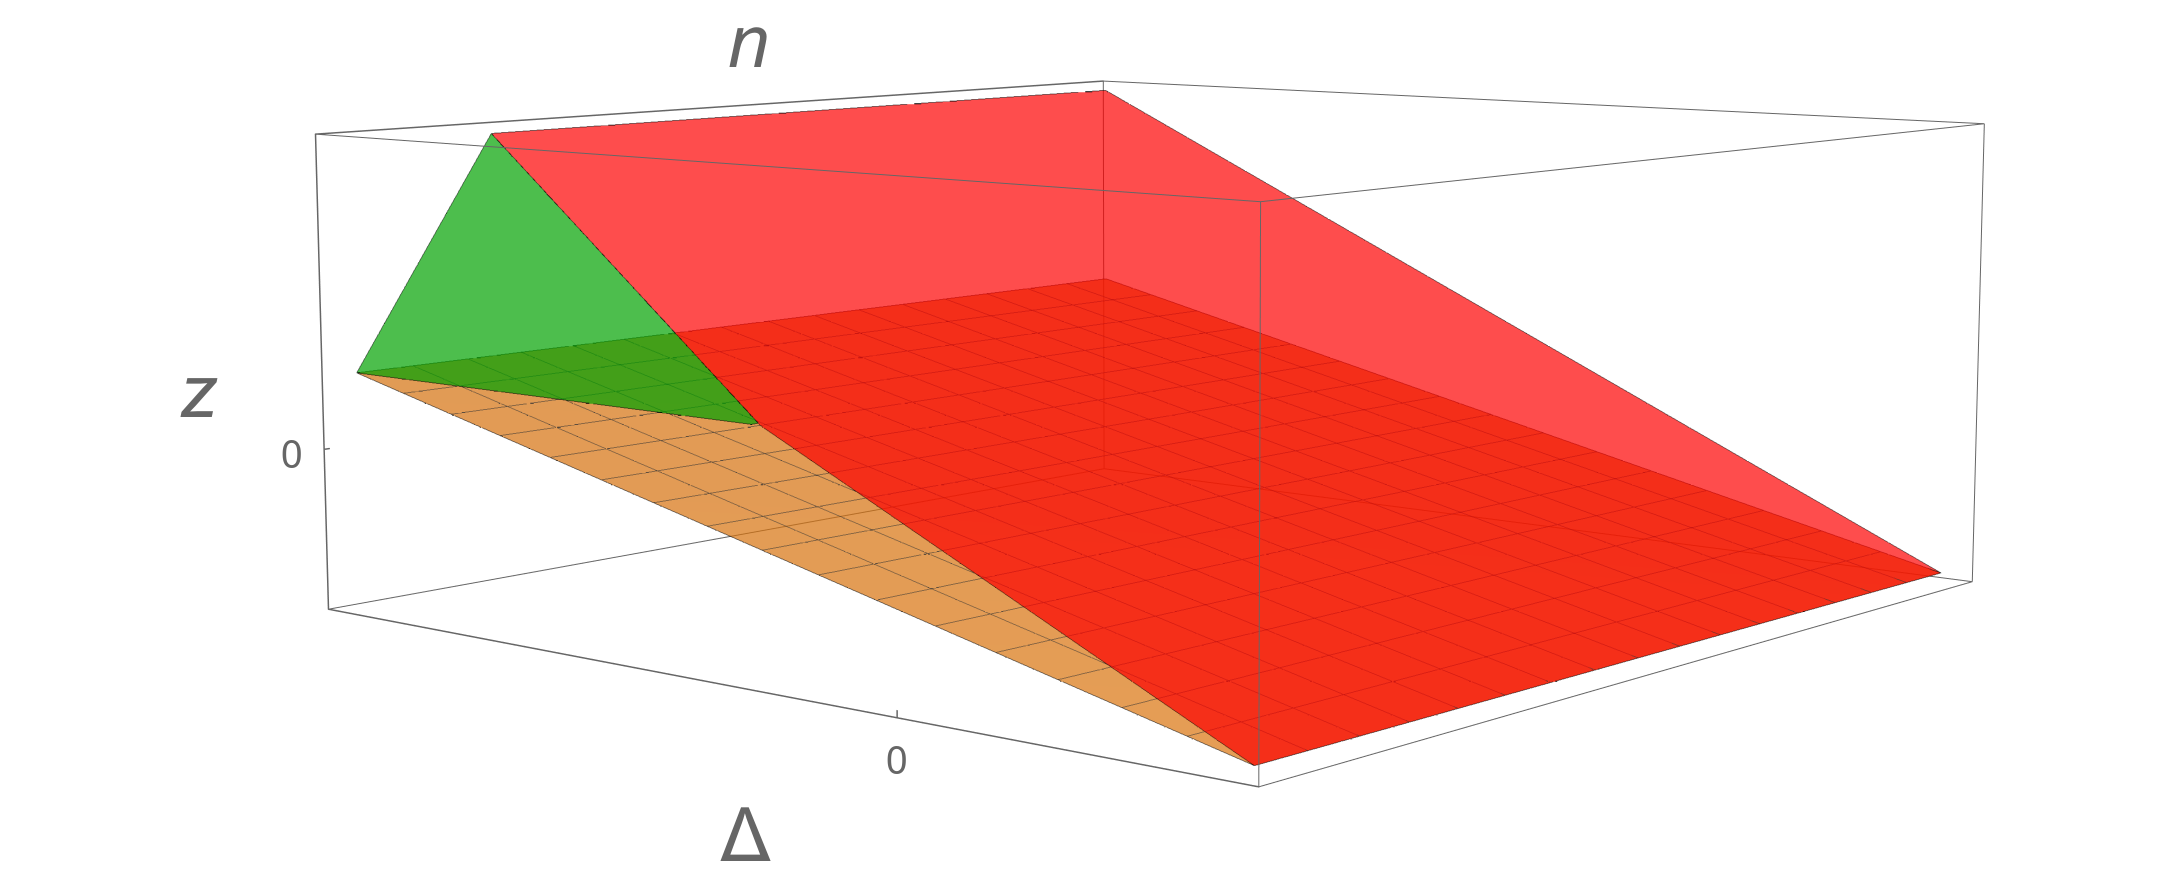
\includegraphics[width=\linewidth]{neurodiff/figs/specialcase2.png}
		\caption{Tighter lower bounding plane.}
		\label{neurodiff:fig:specialcase2}
	\end{minipage}
\end{figure*}
%
%\begin{figure}
%	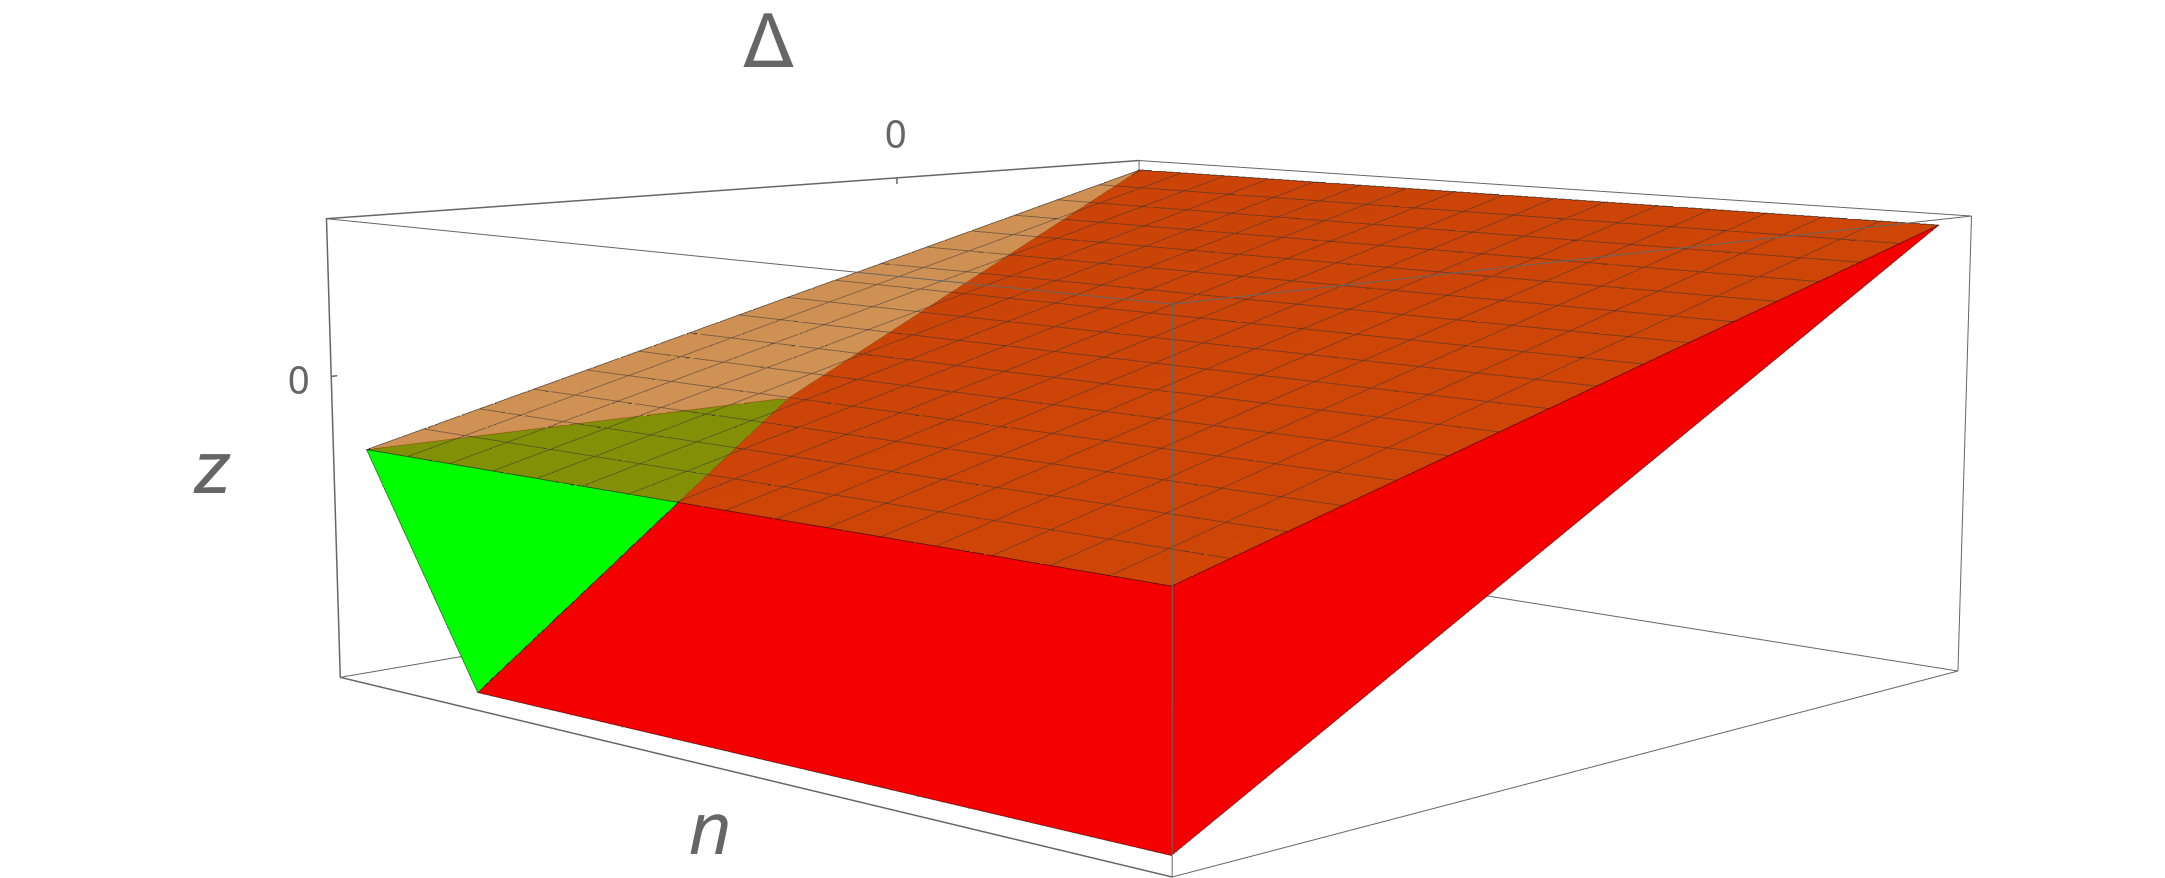
\includegraphics[width=\linewidth]{neurodiff/figs/specialcase1.png}
%	\caption{Tighter upper bounding plane.\label{neurodiff:fig:specialcase1}}
%\end{figure}
%
%\begin{figure}
%	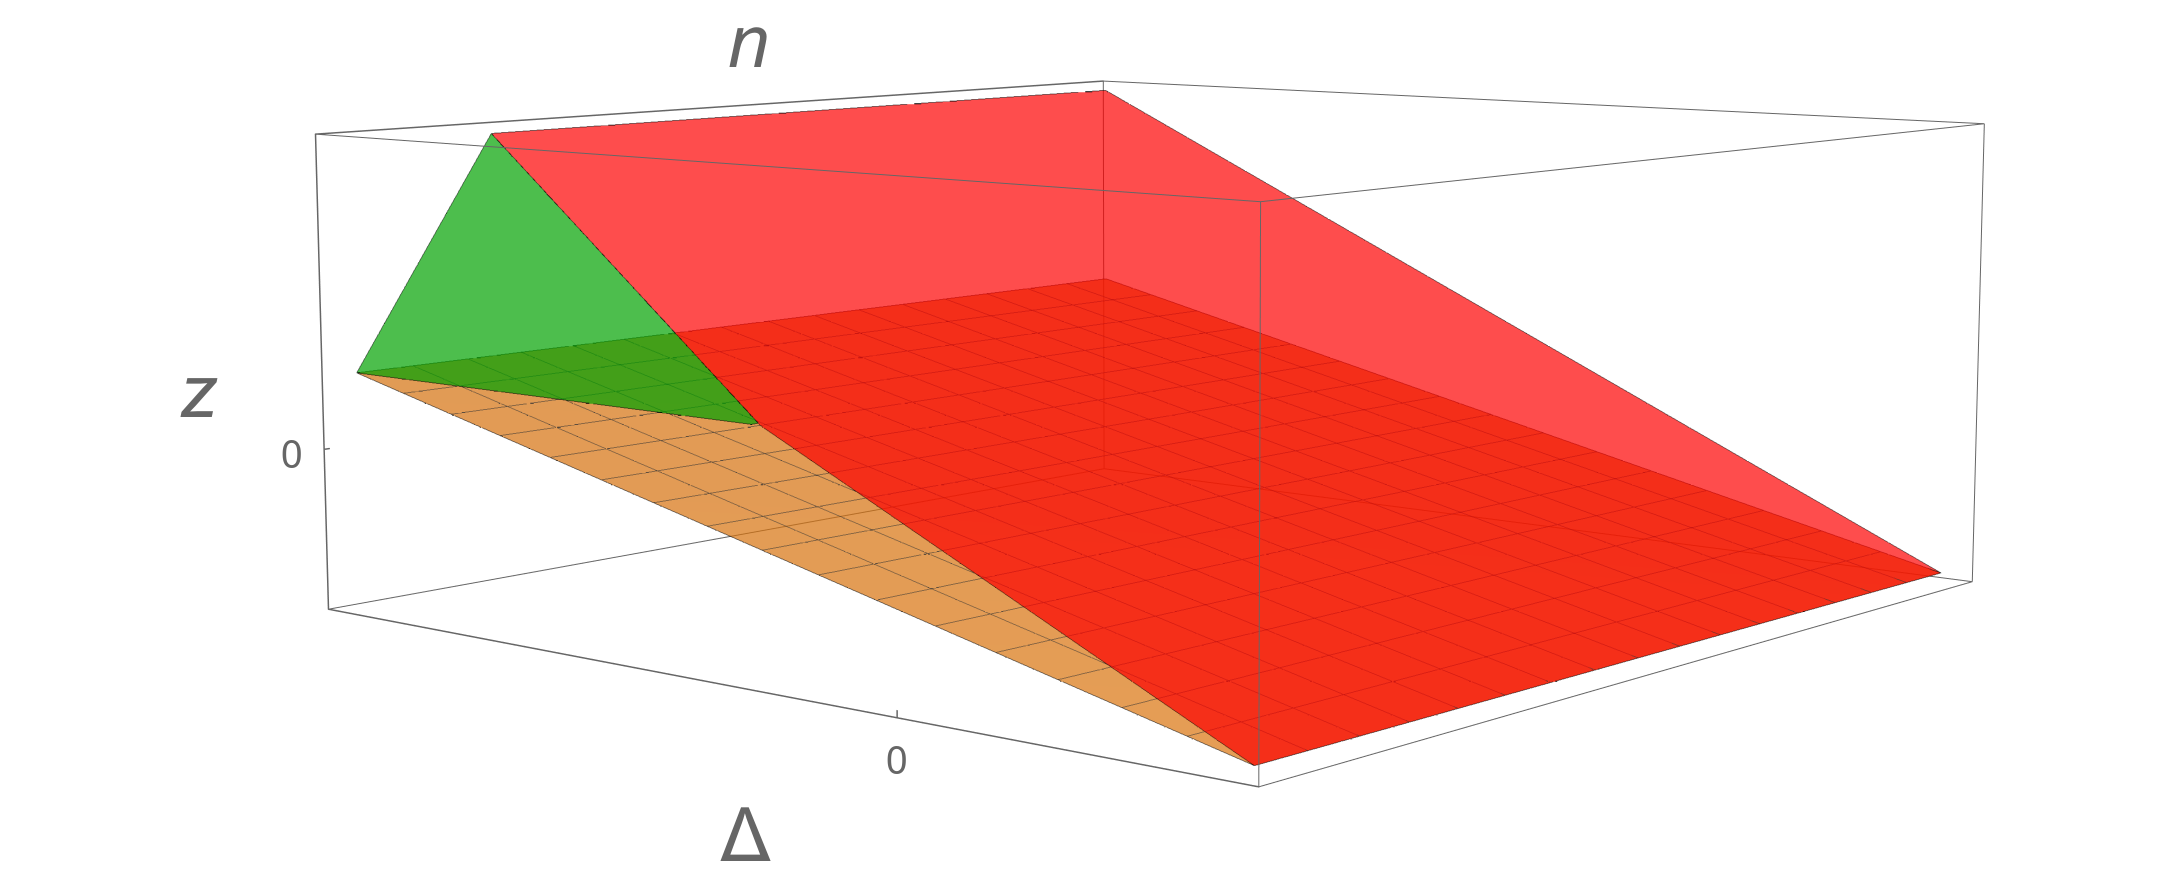
\includegraphics[width=\linewidth]{neurodiff/figs/specialcase2.png}
%	\caption{Tighter lower bounding plane.\label{neurodiff:fig:specialcase2}}
%\end{figure}

\paragraph{Tighter Upper Bound When $ \nn $ Is Linear, $ \UBL{\IntIn{\nnd}}
\leq $  $-\LBL{\IntIn{\nn}} $ $ \leq \UBU{\IntIn{\nnd}} $.}
We illustrate the $ z_1 $ plane under these constraints in
Figure~\ref{neurodiff:fig:specialcase1}.
Let $ l = \UBL{\IntIn{\nnd}} $, and let $ u = \UBU{\IntIn{\nnd}} $, and $ l' =
-\LBL{\IntIn{\nn}} $, we use Lemma~\ref{neurodiff:lemma:1} to derive
$ \UBEq{\IntOut{\nnd}} =$ $ (\UBEq{\IntIn{\nnd}} - l)*\frac{u - l'}{u
- l} + l' $. This results in the upper plane of
Figure~\ref{neurodiff:fig:specialcase1}.
This improves over the third case in our general upper
bound because it allows the lower bound of $ \UBEq{\IntOut{\nnd}} $ to
be less than 0.

\begin{proof}
By our case assumption, Equation~\ref{neurodiff:eq:1} simplifies to the one in
Lemma~\ref{neurodiff:lemma:prev1}. By Lemma~\ref{neurodiff:lemma:1}, we have for
all $ x \in X $,
$ \UBEq{\IntOut{\nnd}}(x) \geq -\LBL{\IntIn{\nn}} $ and
$ \UBEq{\IntOut{\nnd}}(x) \geq \UBEq{\IntIn{\nnd}}(x) $. These two inequalities
imply $ \UBEq{\IntOut{\nnd}} \geq max(-\nn, \nnd) $.
\end{proof}

\paragraph{Tighter Lower Bound When $ \nn $ Is Linear.}

We can use the approximation $ \LBEq{\IntOut{\nnd}}
= \LBEq{\IntIn{\nnd}} $. This improves over the second and third cases
of our general lower bound.

\begin{proof}
By our case assumption, Equation~\ref{neurodiff:eq:1} simplifies to the one in
Lemma~\ref{neurodiff:lemma:prev1}. Thus, $ z_1 = max(-\nn, \nnd) $ $ \implies $
$ z_1 \geq \nnd $.
\end{proof}

\paragraph{Tighter Lower Bound when $ \nnp $ is Linear, $ \LBL{\IntIn{\nnd}}
$ $ \leq \LBL{\IntIn{\nnp}} $ $ \leq \LBU{\IntIn{\nnd}}$.}
We illustrate the $ z_2 $ plane under these constraints in
Figure~\ref{neurodiff:fig:specialcase2}.
Here, letting $ l = \LBL{\IntIn{\nnd}} $, $ u = \LBU{\IntIn{\nnd}} $,
and $ u' = \LBL{\IntIn{\nnp}} $, we can use Lemma~\ref{neurodiff:lemma:2} to
derive the approximation $ \LBEq{\IntOut{\nnd}} $ $ =
(\LBEq{\IntIn{\nnd}} - u)*\frac{u - l'}{u - l} + u' $. This results in the
lower plane of Figure~\ref{neurodiff:fig:specialcase2}. This improves
over the third case, since it allows the upper bound to be greater
than 0.

\begin{proof}
By our case assumption, Equation~\ref{neurodiff:eq:2} simplifies to the one shown
in
Lemma~\ref{neurodiff:lemma:prev2}. By Lemma~\ref{neurodiff:lemma:2}, we have for
all $ x \in X $,
$ \LBEq{\IntOut{\nnd}}(x) \leq \LBEq{\IntIn{\nnd}}(x) $ and
$ \LBEq{\IntOut{\nnd}}(x) \leq \LBL{\IntIn{\nnp}} $. These two inequalities
imply
$ \LBEq{\IntOut{\nnd}}(x)$ $ \leq min(\nnp, \nnd) $.
\end{proof}


\subsection{Intermediate Symbolic Variables for $\IntOut{\nnd}$}
\label{neurodiff:sec:symbolic}


While convex approximations reduce the error introduced by ReLU, even
small errors tend to be amplified significantly after a few layers.
To combat the error explosion, we introduce new symbolic terms to represent the
output values of unstable neurons, which allow their accumulated
errors to cancel out.


We illustrate the impact of symbolic variables on $ \n{1}{1} $ of our
motivating example. Recall we have $ \IntOut{\nd{1}{1}} =$$ [0.05x_1 -
0.05x_2 - 0.2,$ $ 0.05x_1 - 0.05x_2 + 0.2] $. After applying the
convex approximation, we introduce a new variable $ x_3$
such that $ x_3 = $ $ [0.05x_1 - 0.05x_2 - 0.2, $ $
0.05x_1 - 0.05x_2 + 0.2 ]$.
Then we set $ \IntOut{\nd{1}{1}} = [x_3, x_3] $, and
propagate this interval as before. After propagating through
$ \n{2}{1} $ and $ \n{2}{2} $ and combining them at $ \n{3}{1} $, the
$ x_3 $ terms partially cancel out, resulting in the tighter final
output interval $ [-1.65, 1.18] $.

In principle, symbolic variables may be introduced at any unstable
neurons that introduce approximation errors,
however there are efficiency vs. accuracy tradeoffs when
introducing these symbolic variables.  One consideration
is how to deal with intermediate variables referencing other
intermediate variables. For example, if we decide to introduce a
variable $ x_4 $ for $ \n{2}{1} $, then $ x_4 $ will have an $ x_3 $
term in its equation. Then, when we are evaluating a symbolic bound that
contains
an $ x_4 $ term, which will be the case for $ \n{3}{1} $, we will have to
recursively substitute the bounds of the
previous intermediate variables, such as $ x_3 $. This becomes expensive,
especially when it is used together with our bisection-based
refinement~\cite{WangPWYJ18,paulsen2020reludiff}.
%
Thus, in practice, we first remove any back-references to intermediate
variables by substituting in their lower bounds and upper bounds into the
new intermediate variable's lower and upper bounds, respectively.

Given that we do not allow back-references, there are two
additional considerations.
%
First, we must consider that introducing a new intermediate
variable wipes out all the other intermediate variables.  For
example, introducing a new variable at $ \n{2}{1} $ wipes out references
to $ x_3 $, thus preventing any $ x_3 $ terms from canceling at $ \n{3}{1} $.
%
Second, the runtime cost of introducing symbolic variables is not
negligible. The bulk of computation time in \Name{} is spent
multiplying the network's weight matrices by the neuron's symbolic
bound equations, which is implemented using matrix multiplication. Since adding
variables increases the matrix size, this increases the matrix
multiplication cost.

Based on these considerations, we have developed heuristics for adding
new variables judiciously.
%
First, since the errors introduced by unstable neurons in
the \emph{earliest} layers are the most prone to explode, and hence
benefit the most when we create variables for them, we
rank them higher when choosing where to add symbolic variables.
%
Second, we bound the total number of symbolic variables that may be
added, since our experience shows that introducing symbolic variables
for the earliest $ N $ unstable neurons gives drastic improvements in
both run time and accuracy.
%
In practice, $N$ is set to a number proportional
to the weighted sum of unstable neurons in all layers. Formally,
$N=\Sigma_{k=1}^L \gamma^k \times N_k$, where $N_k$ is the number of
unstable neurons in layer $k$ and $\gamma^k = \frac{1}{k}$ is the discount
factor.
%
%\cwnote{Seriously, we have to fix $N$ in our tool, one way or
%another.  The reason is becuase changing $N$ for each benchmark
%arbitrarily sounds really bad!}



\section{Experiments}
\label{neurodiff:sec:experiment}

% Experiments we want to cover
% - ACAS
% 	- eps = 0.05, 0.01
%	- One big table or two small tables
% - MNIST
% 	- 4x1024
%		- increasing perturbation
%		- increasing number of pixels
%		- accuracy on perturb = 8
%	- 6x500
%		- increasing perturbation
%	- Have one line graph for increasing perturbs on both arches
%	- Also do an accuracy comparison for both arches

We have implemented \Name{} and compared it
with \ReluDiff{}~\cite{paulsen2020reludiff}, the state-of-the-art tool for
differential verification of neural networks.
%
\Name{} builds upon the codebase of \ReluDiff{}~\cite{reludiffrepo},
which was also used by single-network verification tools such
as \ReluVal{}~\cite{WangPWYJ18} and \Neurify{}~\cite{WangPWYJ18nips}.
All use OpenBLAS~\cite{ZhangWZ12} to optimize the symbolic
interval arithmetic (namely in applying the weight matrices to the
symbolic intervals).
%
We note that \Name{} uses the algorithm from \Neurify{} to compute
$ \IntOut{\nj} $ and $ \IntOut{\npj} $, whereas \ReluDiff{} uses
the algorithm of \ReluVal{}. Since \Neurify{} is known to compute
tighter bounds than \ReluVal{}~\cite{WangPWYJ18nips},
we compare to both \ReluDiff{}, and an upgraded version of \ReluDiff{}
which uses the bounds from \Neurify{} to ensure
that any performance gain is due to our optimizations and not due to
using \Neurify{}'s bounds. We use the name \ReluDiffP{} to refer
to \ReluDiff{} upgraded with \Neurify{}'s bounds.
%We also
%improved \ReluDiff{} to use a more accurate algorithm for computing
%the absolute values: the original \ReluDiff{} uses the algorithm
%from \ReluVal{}~\cite{WangPWYJ18} to compute $ \IntOut{\nj} $ and
%$ \IntOut{\npj} $, whereas the improved \ReluDiff{} uses the more
%accurate algorithm from \Neurify{}~\cite{WangPWYJ18nips}.
%
%Since our \Name{} also uses the more accurate algorithm
%from \Neurify{}, upgrading \ReluDiff{} to \ReluDiffP{} (the new
%version) allows us to have a more fair experimental comparison.


%To sum up, both \ReluDiff{}/\ReluDiffP{} and \Name{} take two
%structurally similiar networks $ f $ and $ f' $, an input region $ X
%$, and a small $ \epsilon $ value. They then attempt to prove that
%$ \forall x \in X$. $|f'(x) - f(x)| < \epsilon $ for each of the
%network's output nodes.


\subsection{Benchmarks}

Our benchmarks consist of the 49 feed-forward neural networks used by
Paulsen et al.~\cite{paulsen2020reludiff}, taken from three applications:
aircraft collision avoidance, image classification, and human activity
recognition. We briefly describe them here. As in Paulsen et
al.~\cite{paulsen2020reludiff}, the second
network $ f' $ is generated by truncating the edge weights of $f$ from
32 bit to 16 bit floats.

\paragraph{ACAS Xu~\cite{JulianKO18}}
ACAS (aircraft collision avoidance system) Xu is a set of
forty-five neural networks, each with five inputs, six hidden layers of 50 units each, and five outputs,
designed to advise a pilot (the ownship) how to steer an aircraft in the presence of an intruder aircraft.
The inputs describe the position and speed of the intruder relative to the ownship, and the
outputs represent scores for different actions that the ownship should take.
The scores range from $ [-0.5, 0.5] $. We use the input regions defined by the properties of previous
work~\cite{KatzBDJK17, WangPWYJ18}.

\paragraph{MNIST~\cite{LecunBBH98}}
MNIST is a standard image classification task, where the goal is to
correctly classify $ 28 \times 28 $ pixel greyscale images of handwritten
digits. Neural networks trained for this task take 784 inputs (one for
each pixel) each in the range $ [0,255] $, and compute ten outputs -- one
score for each of the ten possible digits. We use three networks of size
3x100 (three hidden layers of 100 neurons each), 2x512, and 4x1024 taken from Weng et al.~\cite{WengZCSHDBD18} and
Wang et al.\cite{WangPWYJ18nips}. All achieve at least 95\% accuracy on
holdout test data.

\paragraph{Human Activity Recognition (HAR)~\cite{AnguitaHAR}}
The goal for this task is to classify
the current activity of human (e.g. walking, sitting, laying down) based
on statistics from a smartphone's gyroscopic sensors. Networks trained
on this task take 561 statistics computed from the sensors and output six
scores for six different activities. We use a 1x500 network.

\subsection{Experimental Setup}

Our experiments aim to answer the following research questions:

\begin{enumerate}
	\item Is \Name{} significantly faster than state-of-the-art?
	\item Is \Name{}'s forward pass significantly more accurate?
	\item Can \Name{} handle significantly larger input regions?
	\item How much does each technique contribute to the overall improvement?
\end{enumerate}

To answer these questions, we run both \Name{}
and \ReluDiff{}/\ReluDiffP{} on all benchmarks and compare their
results.  Both \Name{} and \ReluDiff{}/\ReluDiffP{} can be
parallelized to use multithreading, so we configure a maximum of 12
threads for all experiments.  Our experiments are run on a computer
with an AMD Ryzen Threadripper 2950X 16-core processor, with a
30-minute timeout per differential verification task.


While we could try and adapt a single-network verification tool to our
task as done previously~\cite{paulsen2020reludiff}, we note that \ReluDiff{}
has been shown to significantly outperform (by several orders of
magnitude) this naive approach.



\subsection{Results}

In the remainder of this section, we present our experimental results
in two steps.  First, we present the overall verification results on
all benchmarks. Then, we focus on the detailed verification results on
the more difficult verification tasks.


\subsubsection{Summary of Results on All Benchmarks}


Our experimental results show that, on all benchmarks, the
improved \ReluDiffP{} slightly but consistently outperforms the
original \ReluDiff{} due to its use of the more accurate component
from \Neurify{} instead of \ReluVal{} for bounding the absolute values
of individual neurons.  Thus, to save space, we will only show the
results that compare \Name{} (our method) and \ReluDiffP{}.


\begin{figure}
\centering
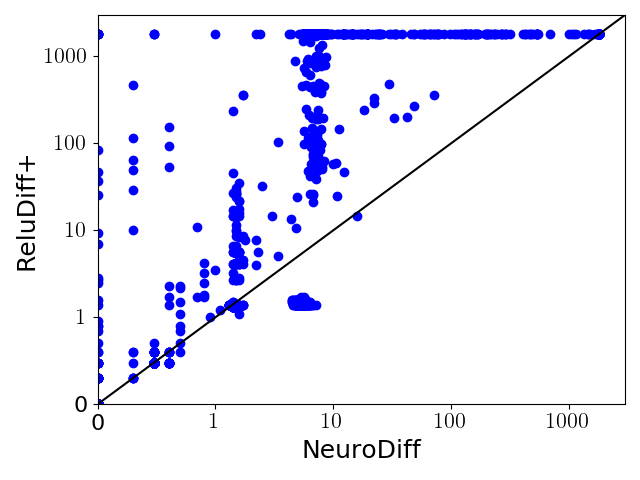
\includegraphics[width=0.7\linewidth]{neurodiff/figs/exp_summary.png}
\caption{Comparing the execution times of \Name{} and \ReluDiffP{} on all verification tasks.}
\label{neurodiff:fig:expsummary}
\end{figure}


We summarize the comparison between \Name{} and \ReluDiffP{} using a
scatter plot in Figure~\ref{neurodiff:fig:expsummary}, where each point
represents a differential verification task: the x-axis is the
execution time of \Name{} in seconds, and the y-axis the execution
time of \ReluDiffP{} in seconds.  Thus, points on the diagonal line
are ties, while points above the diagonal line are wins for \Name{}.


The results show that \Name{} outperformed \ReluDiffP{} for most
verification tasks.  Since the execution time is in logrithmic scale
 the speedups of \Name{} are more
than 1000X for many of these verification tasks.
%
While there are cases where \Name{} is slower than \ReluDiffP{}, due
to the overhead of adding symbolic variables, the differences are on the
order of seconds.  Since they are all on the small MNIST networks and the
HAR network that are very easy for both tools, we omit
an in-depth analysis of them.


In the remainder of this section, we present an in-depth analysis of
the more difficult verification tasks.



\subsubsection{Results on ACAS Networks}


\begin{table}
	\centering
\caption{Results for ACAS networks with $ \epsilon = 0.05 $.}
\label{neurodiff:tbl:acas_orig}
		\begin{tabular}{|c|ccc|ccc|c|}\hline
			\multirow{2}{*}{\makecell[c]{Property}} &  \multicolumn{3}{c|}{\Name{} (new)}
			& \multicolumn{3}{c|}{\ReluDiffP{}} & \multirow{2}{*}{Speedup} \\
			\cline{2-7}
			& proved  & undet. & time (s) & proved & undet. & time (s) &  \\\hline
			\hline

        $\varphi_{1}$   & 45    & 0     & 522.6         & 44    & 1     & 4800.6        &   9.2         \\\hline
$\varphi_{3}$   & 42    & 0     &   2.3         & 42    & 0     &   4.1         &   1.8         \\\hline
$\varphi_{4}$   & 42    & 0     &   1.7         & 42    & 0     &   2.8         &   1.7         \\\hline
$\varphi_{5}$   & 1     & 0     &   0.2         & 1     & 0     &   0.2         &   1.4         \\\hline
$\varphi_{6}$  & 2     & 0     &   0.6         & 2     & 0     &   0.4         &   0.7         \\\hline
$\varphi_{7}$   & 1     & 0     & 1404.4        & 0     & 1     & 1800.0        &   1.3         \\\hline
$\varphi_{8}$   & 1     & 0     & 132.2         & 1     & 0     & 361.8         &   2.7         \\\hline
$\varphi_{9}$   & 1     & 0     &   0.6         & 1     & 0     &   2.3         &   3.7         \\\hline
$\varphi_{10}$  & 1     & 0     &   0.9         & 1     & 0     &   0.7         &   0.8         \\\hline
$\varphi_{11}$  & 1     & 0     &   0.2         & 1     & 0     &   0.3         &   1.6         \\\hline
$\varphi_{12}$  & 1     & 0     &   2.8         & 1     & 0     & 360.9         & 129.4         \\\hline
$\varphi_{13}$  & 1     & 0     &   5.8         & 1     & 0     &   5.1         &   0.9         \\\hline
$\varphi_{14}$  & 2     & 0     &   0.5         & 2     & 0     &  95.9         & 196.2         \\\hline
$\varphi_{15}$  & 2     & 0     &   0.6         & 2     & 0     &  65.0         & 113.2         \\\hline

		\end{tabular}
\end{table}

\begin{table}
	\centering
\caption{Results for ACAS networks with $ \epsilon = 0.01 $.}
\label{neurodiff:tbl:acas_new}
		\begin{tabular}{|c|ccc|ccc|c|}\hline
			\multirow{2}{*}{\makecell[c]{Property}} &  \multicolumn{3}{c|}{\Name{} (new)}
			& \multicolumn{3}{c|}{\ReluDiffP{}} & \multirow{2}{*}{Speedup} \\
			\cline{2-7}
			& proved  & undet. & time (s) & proved & undet. & time (s) &  \\\hline
			\hline

        $\varphi_{1}$   & 41    & 4     & 11400.1       & 15    & 30    & 55778.6       &   4.9         \\\hline
$\varphi_{3}$   & 42    & 0     &  14.3         & 35    & 7     & 13642.2       & 957.2         \\\hline
$\varphi_{4}$   & 42    & 0     &   3.8         & 37    & 5     & 9115.0        & 2390.1        \\\hline
$\varphi_{5}$   & 1     & 0     &   0.3         & 0     & 1     & 1800.0        & 5520.5        \\\hline
$\varphi_{16}$  & 2     & 0     &   1.0         & 2     & 0     &   0.8         &   0.8         \\\hline
$\varphi_{7}$   & 0     & 1     & 1800.0        & 0     & 1     & 1800.0        &   1.0         \\\hline
$\varphi_{8}$   & 1     & 0     & 1115.9        & 0     & 1     & 1800.0        &   1.6         \\\hline
$\varphi_{9}$   & 1     & 0     &   2.4         & 0     & 1     & 1800.0        & 738.2         \\\hline
$\varphi_{10}$  & 1     & 0     &   1.6         & 1     & 0     &   1.1         &   0.7         \\\hline
$\varphi_{11}$  & 1     & 0     &   0.3         & 0     & 1     & 1800.0        & 5673.8        \\\hline
$\varphi_{12}$  & 1     & 0     & 132.2         & 0     & 1     & 1800.0        &  13.6         \\\hline
$\varphi_{13}$  & 1     & 0     &  15.9         & 1     & 0     &  14.8         &   0.9         \\\hline
$\varphi_{14}$  & 2     & 0     & 1589.3        & 0     & 2     & 3600.0        &   2.3         \\\hline
$\varphi_{15}$  & 2     & 0     & 579.4         & 0     & 2     & 3600.0        &   6.2         \\\hline

		\end{tabular}
\end{table}


For ACAS networks, we consider two different sets of properties,
namely the original properties from Paulsen et al.~\cite{paulsen2020reludiff}
where $ \epsilon = 0.05 $, and the same properties but with $ \epsilon
= 0.01 $.  We emphasize that, while verifying $ \epsilon = 0.05 $ is
useful, this means that the output value can vary by up to
10\%. Considering $ \epsilon = 0.01 $ means that the output value can
vary by up to 2\%, which is much more useful.
%For all properties, we
%let \Name{} use up to 15 intermediate variables. We tuned the number
%on property $ \varphi_1 $ on the first of the 45 networks
%(i.e. network 1\_1).

Our results are shown in Tables~\ref{neurodiff:tbl:acas_orig}
and~\ref{neurodiff:tbl:acas_new}, where the first column shows the property,
which defines the input space considered. The next three columns show
the results for \Name{}, specifically the number of verified networks
(out of the 45 networks), the number of unverified networks, and the
total run time across all networks. The next three show the same
results, but for \ReluDiffP{}. The final column shows the average
speed up of \Name{}.

The results show that \Name{} makes significant gains in both speed
and accuracy. Specifically, the speedups are up to two and three
orders of magnitude for $ \epsilon = 0.05 $ and $ 0.01 $,
respectively. In addition, at the more accurate $ \epsilon = 0.01 $
level, \Name{} is able to complete 53 more verification tasks, out of
the total 142 verification tasks.


\subsubsection{Results on MNIST Networks}

\begin{figure*}[t]
\centering
	\begin{minipage}[t]{0.498\linewidth}
        \centering
		\captionsetup{width=0.9\textwidth}
		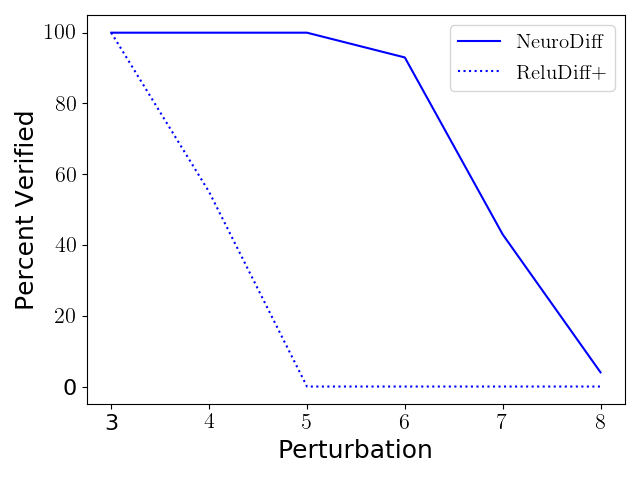
\includegraphics[width=.99\linewidth]{neurodiff/figs/4x1024_comp.png}
		\caption{Percentage of verification tasks completed on the MNIST 4x1024
		network for various perturbations.\label{neurodiff:fig:perturbation_comp}}
	\end{minipage}%
	\begin{minipage}[t]{0.498\linewidth}
        \centering
		\captionsetup{width=0.9\textwidth}
		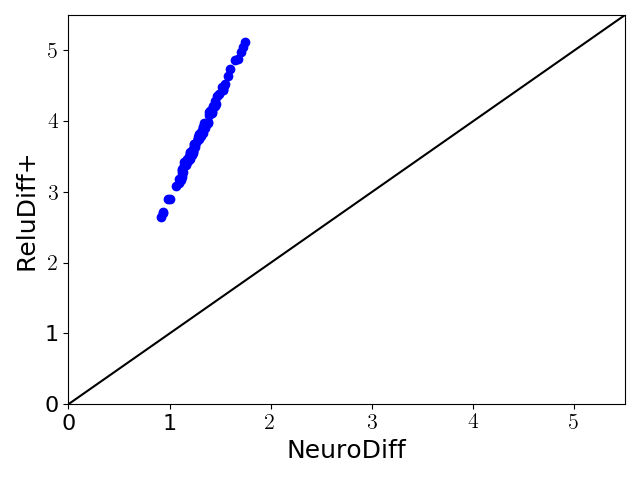
\includegraphics[width=.99\linewidth]{neurodiff/figs/mnist_4x1024_scatterplot.png}
		\caption{Accuracy comparison for a single forward pass on the MNIST 4x1024
		network with perturbation of 8.\label{neurodiff:fig:accuracy_comp}}
	\end{minipage}%
\end{figure*}

For MNIST, we focus on the 4x1024 network, which is the largest
network considered by Paulsen et al.~\cite{paulsen2020reludiff}.  In contrast,
since the smaller networks, namely 3x100 and 2x512 networks, were
handled easily by both tools, we omit their results.
%
In the MNIST-related verification tasks, the goal is to verify
$ \epsilon = 1 $ for the given input region. We consider the two types
of input regions from the previous work, namely global perturbations
and targeted pixel perturbations, however we use input regions that
are hundreds of orders of magnitude larger.
%For all verification
%tasks, we allow 1,000 intermediate variables for \Name{}. We tuned the
%number on the first of our global perturbation properties.

First, we look at the global perturbation. For these, the input space
is created by taking an input image and then allowing a perturbation
of +/- $ p $ greyscale units to all of its pixels. In the previous
work, the largest perturbation was $ p = 3$.
%
Figure~\ref{neurodiff:fig:perturbation_comp} compares \Name{} and \ReluDiffP{}
on $ p = 3 $ all the way up to 8, where the x-axis is the perturbation
applied, and the y-axis is the percentage of verification tasks (out
of 100) that each can handle.


The results show that \Name{} can handle perturbations up to +/-
6 units, whereas \ReluDiffP{} begins to struggle at 4. While the
difference between 4 and 6, may seem small, the volume of input space
for a perturbation of 6 is $ 6^{784}/4^{784} \approx 1.1 \times
10^{138} $ times larger than 4, or in other words, 138 orders of
magnitude larger.


Next, we show a comparison of the epsilon verified by a single forward pass
for a perturbation of 8 on the MNIST 4x1024 network in
Figure~\ref{neurodiff:fig:accuracy_comp}.
Points above the blue line indicate \Name{} performed
better. Overall, \Name{} is between two and three times more accurate
than \ReluDiffP{}.

Finally, we look at the targeted pixel perturbation properties. For
these, the input space is created by taking an image, randomly
choosing $ n $ pixels, and setting there bounds to $ [0,255] $, i.e.,
allowing arbitrary changes to the chosen pixels. We again use the
4x1024 MNIST network. The results are summarized in
Table~\ref{neurodiff:tbl:MNIST_pix}. The first column shows the number of
randomly perturbed pixels. We can again see very large speedups, and a
significant increase in the size of the input region that \Name{} can
handle.


\begin{table}
	\centering
	\caption{Results of the MNIST 4x1024  pixel experiment.}
	\label{neurodiff:tbl:MNIST_pix}
	\scalebox{1.0}{
		\begin{tabular}{|c|ccc|ccc|c|}\hline
			\multirow{2}{*}{\makecell[c]{Num. \\ Pixels}} &  \multicolumn{3}{c|}{\Name{} (new)}
			& \multicolumn{3}{c|}{\ReluDiffP{}} & \multirow{2}{*}{Speedup} \\
			\cline{2-7}
			& proved  & undet. & time (s) & proved & undet. & time (s) &  \\\hline
			\hline

15      & 100   & 0     & 236.5 & 100   & 0     & 1610.2        &   6.8 \\\hline
18      & 100   & 0     & 540.8 & 88    & 12    & 34505.8       &  63.8 \\\hline
21      & 100   & 0     & 1004.0        & 30    & 70    & 145064.5      & 144.5 \\\hline
24      & 99    & 1     & 7860.1        & 1     & 99    & 179715.9      &  22.9 \\\hline
27      & 83    & 17    & 49824.0       & 0     & 100   & 180000.0      &   3.6 \\\hline


		\end{tabular}
	}
\end{table}


\subsubsection{Contribution of Each Technique}

Here, we analyze the contribution of individual techniques, namely
convex approximations and symbolic variables, to the overall
performance improvement.

%We look at the benefit in two of our experiments: the ACAS
%experiments with $ \epsilon = 0.01 $ presented in
%Table~\ref{neurodiff:tbl:acas_comp} and MNIST with varying degrees of global
%perturbations presented in Table~\ref{neurodiff:tbl:MNIST_comp}.


\begin{comment}
In Table~\ref{neurodiff:tbl:acas_comp}, we compare the performance of \Name{}
with both techniques enabled and \Name{} with only intermediate
variables. The right most column essentially shows the speedup with
the addition convex approximations. Overall we can see that the
speedup is relatively small, and that the intermediate variables do
most of the heavy-lifting in the ACAS experiments.


\begin{table}
	\caption{Comparison of full \Name{} and  \Name{} with only symbolic variables
	on ACAS experiments with $ \epsilon = 0.01 $. \label{neurodiff:tbl:acas_comp}}
	\scalebox{0.75}{
		\begin{tabular}{|c|ccc|ccc|c|}\hline
			\multirow{2}{*}{\makecell[c]{Property}} &  \multicolumn{3}{c|}{\Name{}}
			& \multicolumn{3}{c|}{Int. Vars. Only} & \multirow{2}{*}{Speedup} \\
			\cline{2-7}
			& proved  & undet. & time (s) & proved & undet. & time &  \\\hline
			\hline

			$\varphi_{1}$ 	& 40 	& 5 	& 11930.8 	& 40 	& 5 	& 12102.5 	&   1.0 	\\\hline
			$\varphi_{3}$ 	& 42 	& 0 	&  12.0 	& 42 	& 0 	&  46.8 	&   3.9 	\\\hline
			$\varphi_{4}$ 	& 42 	& 0 	&   3.4 	& 42 	& 0 	&   7.9 	&   2.3 	\\\hline
			$\varphi_{5}$ 	& 1 	& 0 	&   0.2 	& 1 	& 0 	&   0.3 	&   1.3 	\\\hline
			$\varphi_{6}$ 	& 2 	& 0 	&   0.6 	& 2 	& 0 	&   0.6 	&   1.1 	\\\hline
			$\varphi_{7}$ 	& 0 	& 1 	& 1800.0 	& 0 	& 1 	& 1800.0 	&   1.0 	\\\hline
			$\varphi_{8}$ 	& 1 	& 0 	& 756.5 	& 1 	& 0 	& 1154.9 	&   1.5 	\\\hline
			$\varphi_{9}$ 	& 1 	& 0 	&   1.8 	& 1 	& 0 	&   3.2 	&   1.8 	\\\hline
			$\varphi_{10}$ 	& 1 	& 0 	&   1.0 	& 1 	& 0 	&   1.1 	&   1.1 	\\\hline
			$\varphi_{11}$ 	& 1 	& 0 	&   0.2 	& 1 	& 0 	&   0.3 	&   1.3 	\\\hline
			$\varphi_{12}$ 	& 1 	& 0 	& 148.5 	& 1 	& 0 	& 228.3 	&   1.5 	\\\hline
			$\varphi_{13}$ 	& 1 	& 0 	&  10.6 	& 1 	& 0 	&  12.6 	&   1.2 	\\\hline
			$\varphi_{14}$ 	& 2 	& 0 	& 1798.0 	& 2 	& 0 	& 2116.3 	&   1.2 	\\\hline
			$\varphi_{15}$ 	& 2 	& 0 	& 513.3 	& 2 	& 0 	& 690.8 	&   1.3 	\\\hline

		\end{tabular}
	}
\end{table}

\end{comment}



In Table~\ref{neurodiff:tbl:MNIST_comp}, we present the average $ \epsilon $
that was able to be verified after a single forward pass on the
4x1024 MNIST network for each of
the four techniques: \ReluDiffP{} (baseline), \Name{} with only convex
approximations, \Name{} with only intermediate variables, and the
full \Name{}.


Overall, the individual benefits of the two proposed approximation
techniques are obvious.  While convex approximation
(alone) consistently provides benefit as perturbation increases, the
benefit of symbolic variables (alone) tends to decrease.
%
In addition, combining the two provides much greater benefit than the
sum of their individual contributions. With perturbation of 8, for
example, convex approximations alone are 1.59 times more accurate than
\ReluDiffP{}, and intermediate variables alone are 1.01 times more accurate.
However, together they are 2.93 times more accurate.


\begin{table}
	\centering
	\caption{Evaluating the individual contributions of convex approximation and symbolic variables using the  MNIST 4x1024 global perturbation experiment.}
	\label{neurodiff:tbl:MNIST_comp}
	\scalebox{1.0}{
		\begin{tabular}{|c|c|c|c|c|}\hline
			\multirow{2}{*}{Perturb} &  \multicolumn{4}{c|}{Average $ \epsilon $ Verified} \\
			\cline{2-5}
			& \ReluDiffP{} & Conv. Approx. & Int. Vars. & \Name{} \\
			\hline
3 & 0.59 & 0.42 (+1.39x) & 0.43 (+1.38x) & 0.20 (+2.93x) \\\hline
4 & 1.02 & 0.70 (+1.46x) & 0.87 (+1.18x) & 0.36 (+2.85x) \\\hline
5 & 1.60 & 1.06 (+1.52x) & 1.47 (+1.09x) & 0.56 (+2.87x) \\\hline
6 & 2.29 & 1.47 (+1.55x) & 2.19 (+1.04x) & 0.79 (+2.90x) \\\hline
7 & 3.02 & 1.92 (+1.58x) & 2.96 (+1.02x) & 1.04 (+2.91x) \\\hline
8 & 3.80 & 2.39 (+1.59x) & 3.77 (+1.01x) & 1.30 (+2.93x) \\\hline
		\end{tabular}
	}
\end{table}


The results suggest two things.
%
First, intermediate
symbolic variables perform well when a significant portion of the
network is already in the stable state.  We confirm, by manually
inspecting the experimental results, that it is indeed the case when
we use a perturbation of 3 and 8 in the MNIST experiments.
%, and we believe
%this is the case for ACAS as well, once the input space is
%sufficiently partitioned.
Second, the convex approximations provide the most benefit when the
pre-ReLU delta intervals are (1) significantly wide, and (2) still
contain a significant amount of symbolic information. This is also
confirmed by manually inspecting our MNIST results: increasing the
perturbation increases the overall width of the delta intervals.
%In
%addition, this is very likely why we do not see a significant benefit
%from convex approximations in the ACAS results. Since the ACAS
%networks have many fewer parameters than the MNIST network, the total
%amount of change in the network from rounding to 16 bits is relatively
%small. This leads to relatively narrow delta intervals, and hence
%there is little opportunity for benefit.

%\subsection{Threats to Validity}
%We note that the refinement of both \Name{} and \ReluDiff{} typically does not work well with large input spaces. However, the LP solving-based refinement of Wang et al.~\cite{WangPWYJ18nips} has been shown to scale better to higher-dimensional input spaces, and could straightforwardly be integrated into \Name{}.
%
%We also focus on feed-forward ReLU networks. ReLU activations are preferable in safety critical systems because they are the most amenable to verification. Still, much previous work~\cite{SinghGPV19, SinghGPV19iclr, zhang2018efficient} has shown that convex approximations can be extended non-linear activations as well. We believe \Name{} can be extended as such too.


%\section{Related Work}
%\label{neurodiff:sec:related}
%
%
%% Single network verification
%% - complete techniques
%Aside from \ReluDiff{}~\cite{paulsen2020reludiff}, the most closely related to
%our work are those that focus on verifying properties of single
%networks as opposed to two or more networks. These verification
%approaches can be broadly categorized into those that use exact,
%constraint solving-based techniques and those that use approximations.
%
%
%On the constraint solving side, several works have adapted
%off-the-shelf solvers~\cite{CarliniW17, tjeng2019evaluating,
%BastaniILVNC16, Ehlers17, baluta2019quantitative}, or even implemented
%solvers specifically for neural networks~\cite{KatzBDJK17,
%KatzHIJLLSTWZDK19}.
%%
%On the approximation side, many use techniques that fit into the framework of
%abstract interpretation~\cite{CousotC77}. For example, many works have leveraged
%abstract domains such as intervals~\cite{WangPWYJ18, WengZCSHDBD18,
%zhang2018efficient, JulianKO18}, polyhedra~\cite{Singh2019krelu, SinghGPV19}, and
%zonotopes~\cite{SinghGPV19iclr, GehrMDTCV18}.
%
%
%In addition, these verification techniques have also been
%combined~\cite{SinghGPV19iclr, WangPWYJ18nips, HuangKWW17}, or
%entirely different approaches~\cite{RuanHK18, DvijothamSGMK18,
%GopinathKPB18}, such as bounding a network's lipschitz constant, have
%been studied. These verification techniques can also be integrated
%into the training process to produce more robust and easier to verify
%networks~\cite{FischerBDGZV19, MirmanGV18, WongK18,
%balunovic2020adversarial}. These works are orthogonal, though we
%believe their techniques can be adapted to our domain.
%
%
%% Various heuristic based approaches, focus on discovering but not proving the
%%absence of adversarial examples
%A related but tangential line of work focuses on discovering
%interesting behaviors of neural networks, though without any
%guarantees.
%%
%Most closely related to our work are differential testing
%techniques~\cite{xie2019diffchaser, PeiCYJ17, MaLLZG18}, which focus
%on finding disagreements between a set of networks.
%%
%However, these techniques do not attempt to prove the equivalence or
%similarity of multiple networks.
%
%Other works are more geared towards single network testing, and use
%white-box testing techniques~\cite{ma2018deepgauge, xie2019deephunter,
%SunWRHKK18, TianPJR18, odena2018tensorfuzz}, such as neuron coverage
%statistics, to assess how well a network has been tested, and also
%report interesting behaviors. Both of these can be thought of as
%adapting software engineering techniques to machine learning.
%
%
%In addition, many works use machine learning techniques, such as
%gradient optimization, to find interesting behaviors, such as
%adversarial examples\cite{KurakinGB17a, madry2017towards, NguyenYC15,
%XuQE16, Moosavi-Dezfooli16}. These interesting behaviors can then be
%used to retrain the network to improve
%robustness~\cite{GoodfellowSS15, RaghunathanSL18}. Again, these
%techniques do not provide guarantees, though we believe they could be
%integrated into \Name{} to quickly find counterexamples.
%
%Finally, our work draws inspiration from classic software engineering
%techniques, such as regression testing~\cite{rothermel1997safe},
%differential assertion checking~\cite{lahiri2013differential},
%differential fuzzing~\cite{NilizadehNP19}, and incremental symbolic
%execution~\cite{Person11,GuoKW16}, where one version of a program is
%used as an ``oracle'', to more efficiently test or verify a new
%version of the same program.  In our case, $ f $ can be thought of as
%the oracle, while $ f' $ is the new version.


\section{Summary}
\label{neurodiff:sec:conclusion}

We have presented \Name{}, a scalable differential verification
technique for soundly bounding the difference between two feed-forward
neural networks. \Name{} leverages novel convex approximations, which
reduce the overall approximation error, and intermediate symbolic
variables, which control the error explosion, to significantly improve
efficiency and accuracy of the analysis. Our experimental evaluation
shows that \Name{} can achieve up to 1000X speedup and is up to five
times as accurate.




\chapter{Online Synthesis of Linear Approximations}
\label{ch:onlinesyn}
\newcommand\bpnote[1]{\textcolor{blue}{{\textbf{Brandon Says: #1}}}}
\declarecommand\jwnote[1]{\textcolor{purple}{{\textbf{Jingbo Says: #1}}}}
\declarecommand\cwnote[1]{\textcolor{red}{{\textbf{Chao Says: #1}}}}

\declarecommand{\Name}{\textsc{LinSyn}}
\declarecommand{\ReluDiff}{\textsc{ReluDiff}}
\declarecommand{\ReluVal}{\textsc{ReluVal}}
\declarecommand{\DeepPoly}{\textsc{DeepPoly}}
\declarecommand{\Reluplex}{\textsc{Reluplex}}
\declarecommand{\Neurify}{\textsc{Neurify}}
\declarecommand{\Crown}{\textsc{Crown}}
\declarecommand{\Popqorn}{\textsc{Popqorn}}
\declarecommand{\RefineZono}{\textsc{RefineZono}}
\declarecommand{\dReal}{\textsc{dReal}}
\declarecommand{\autolipra}{\textsc{AutoLiRPA}}
\declarecommand{\popqorn}{\textsc{POPQORN}}

\declarecommand{\nj}[0]{n_{k,j}}
\declarecommand{\n}[2]{n_{#1,#2}}
\declarecommand{\np}[2]{n'_{#1,#2}}
\declarecommand{\npj}[0]{n'_{k,j}}
\declarecommand{\nd}[2]{\Delta_{#1,#2}}
\declarecommand{\ndj}{\Delta_{k,j}}
\declarecommand{\W}[3]{W_{#1}[#2,#3]}
\declarecommand{\Wp}[3]{W_{#1}'[#2,#3]}
\declarecommand{\Wk}[1]{W_{#1}}
\declarecommand{\Wd}[3]{W_{#1}^\Delta[#2,#3]}

%\subsubsection{\textcolor{red}{There is a need for verifying the robustness of
%neural network...}}
Prior work has shown that neural networks are vulnerable to various types of
(adversarial) perturbations, such as small $l$-norm bounded
perturbations~\cite{szegedy2013intriguing}, geometric
transformations~\cite{engstrom2019exploring,kanbak2018geometric}, and word
substitutions~\cite{alzantot2018generating}. Such perturbations can often
cause a misclassification for any given input, which may have serious
consequences, especially in safety critical systems.
%
Certifying robustness to these perturbations has become an important problem as
it can show the network does not exhibit these misclassifications, and
furthermore
previous work has shown that a given input feature's
certified robustness can be a useful indicator to determine the feature's
importance in the network's decision~\cite{shi2020robustness,ko2019popqorn}.

%\subsubsection{\textcolor{red}{The most scalable approach relies on computing
%symbolic ranges}}
Indeed, many approaches have been proposed for certifying the
robustness of inputs to these perturbations. Previous work typically
leverages two types of techniques: (1) fast and scalable, but approximate
techniques~\cite{SinghGPV19,GehrMDTCV18,WengZCSHDBD18,shi2020robustness,ko2019popqorn},
 and (2) expensive but exact techniques that leverage some type of
constraint
solver~\cite{KatzBDJK17,KatzHIJLLSTWZDK19,tjeng2019evaluating}. Several works
have also
combined the
two~\cite{SinghGPV19iclr,Singh2019krelu,WangPWYJ18nips,tran2019star}. The
most successful approaches, in terms of scalability in practice, are built on top of the approximate techniques, which
all depend on computing \textit{linear bounds} for the non-linear activation functions.

%\begin{itemize}
%\item don't forget to cite papers such as ReluPlex
%\item don't forget to cite papers such as ReluVal and DeepPoly
%\item cite other important papers as well
%\end{itemize}

%\subsubsection{\textcolor{red}{However, existing techniques for computing the
%linear bounds have limitations}}

However, a key limitation is that the linear bounds must be handcrafted and
proven sound by experts. Not only is this process difficult, but also ensuring
the tightness of the crafted bounds presents an additional challenge.
Unfortunately, prior work has only crafted bounds for the most common
activation functions and architectures, namely ReLU~\cite{WangPWYJ18nips},
sigmoid, tanh~\cite{SinghGPV19,zhang2018efficient,wu2021tightening}, the exp
function~\cite{shi2020robustness}, and some
2-dimensional activations found in LSTM networks~\cite{ko2019popqorn}.
%
As a result, existing tools for neural network verification
cannot handle a large number of activation functions that are
frequently used in practice.  Examples include the \emph{GELU}
function~\cite{hendrycks2016gaussian}, which is currently the activation
function used in OpenAI's GPT~\cite{radford2018improving}, and the \emph{Swish}
function which has been shown to outperform the standard ReLU function in some
applications~\cite{ramachandran2017searching} and, in particular, can reduce
over-fitting in adversarial training~\cite{singla2021low}. In addition, these
recently introduced activation
functions are often significantly more complex than previous activation
functions, e.g., we have $
\mathit{gelu}(x) = 0.5 x ( 1 + \tanh{[ \sqrt{2 / \pi } (x + 0.044715x ^{3} ) ]
} )
$.
%
%In addition, even for activation functions that can be handled by
%existing tools, many of the hand-crafted bounds are suboptimal and/or
%do not come with tightness guarantees.

%\begin{itemize}
%	\item They require linear bounds to be provided by experts
%	\item The bounds can be difficult to craft, e.g. the best known bounds for
%LSTM activations are heuristic
%    \item They are often sub-optimal, i.e., these bounds are not tight enough
%\end{itemize}

%\subsubsection{\textcolor{red}{Problem statement}}



%TODO:
% - change to z = sigma(x)
% - change n to d
In this work, we study the problem of \textit{efficiently} and
\textit{automatically}
synthesizing \textit{sound} and \textit{tight} linear bounds for any
\textit{arbitrary activation function}.
%
By \emph{arbitrary activation function}, we mean \textit{any} (non-linear)
computable function $ z = \sigma(x_1,\dots,x_d) $ used inside a neural network
with $ d $ input variables.
%
By \textit{sound} we mean, given an interval bound on each
variable $ x_1 \in
[l_1, u_1], x_2 \in [l_2, u_2], \dots, x_d \in [l_d, u_d]$, the problem is to \textit{efficiently}
compute lower bound coefficients $ c^l_1, c^l_2, \dots, c^l_{d+1} $, and upper
bound coefficients $ c^u_1, c^u_2, \dots, c^u_{d+1} $ such that the following
holds:
\begin{equation}\label{onlinesyn:eq:intro-sound}
\begin{gathered}
	\forall x_1 \in [l_1, u_1], x_2 \in [l_2, u_2], \dots,  x_d \in [l_d, u_d]\\
	c^l_1x_1 + c^l_2x_2 + \dots + c^l_{d+1}
	\leq \sigma(x_1,\dots,x_d) \leq
	c^u_1x_1 + c^u_2x_2 + \dots + c^u_{d+1}
\end{gathered}
\end{equation}
%
By \textit{automatically}, we mean that the above is done using only the
definition of the activation function itself.
%
Finally, by \textit{tight}, we mean that some formal measure, such as the
volume above/below the linear bound, is minimized/maximized.

\begin{figure}[t]
	%\textcolor{red}{We need to draw a block diagram, to illustrate the three
	%steps
	%of \Name{}.}
	%\vspace{5ex}
	%\textcolor{red}{We also need to show the input to \Name{} (defintion of
	%the
	%activation function, provided \emph{a priori}, and given input region,
	%provide
	%at run time).}
	%\vspace{5ex}
	%\textcolor{red}{Perhaps we can also show how \Name{} fits into a generic
	%verification tool (could be, but doesn't have to be, AutoLiPRA).}
	\centering
	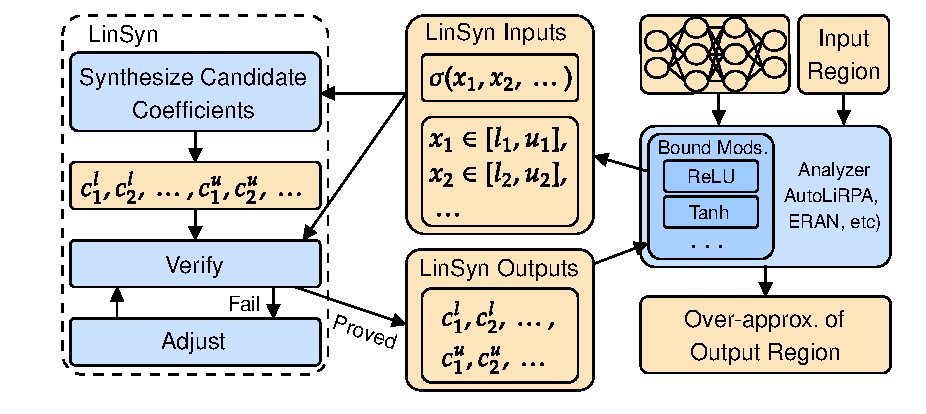
\includegraphics[width=.9\linewidth]{onlinesyn/figs/flow_diagram.pdf}
\caption{The overall flow of~\Name{}.\label{onlinesyn:fig:block-diagram}}
\end{figure}

%\subsubsection{\textcolor{red}{High-level description of our method}}

We have developed a new method, named~\Name{}, that can \emph{automatically}
synthesize tight linear bounds for \emph{any arbitrary} non-linear activation
function $ \sigma(\cdot) $.
%
We illustrate the flow of our method on the left-hand side of
Fig.~\ref{onlinesyn:fig:block-diagram}. As shown,~\Name{} takes two inputs: a
definition of the activation function, and an interval for each of its
inputs.~\Name{} outputs linear coefficients such that
Equation~\ref{onlinesyn:eq:intro-sound} holds.
%
Internally,~\Name{}
uses sampling and an LP (linear programming) solver to synthesize
candidate lower and upper bound coefficients.
Next, it uses an
efficient local minimizer to compute a good estimate of the offset
needed to ensure soundness of the linear bounds.
%
Since the candidate bounding functions constructed in this manner may
still be unsound, finally, we use a highly optimized branch-and-bound
nonlinear SMT solver, named~\dReal{}~\cite{gao2013dreal}, to verify the
soundness of the linear bounds.
%
Even though our new method involves the use of solvers and
optimizers, the entire process typically takes less than 1/100th of a
second per pair of bounds.

Fig.~\ref{onlinesyn:fig:block-diagram} also illustrates how~\Name{} fits in with
existing neural network verification frameworks, such as ERAN~\cite{eran},
and~\autolipra{}~\cite{autolipra}. These tools take as input a neural network,
and a region of the neural networks input space, and compute an
over-approximation of the neural network's outputs. Internally, these
frameworks have modules that compute linear bounds for a specific activation
functions.~\Name{} is a one-size-fits-all drop-in replacement for these modules
that are invoked at runtime whenever a linear bound of a non-linear activation function is needed.
%Furthermore, we propose an optimization that can exploit
%convex/concave regions of $ \sigma $.

% Our approach
% - bound activation without decomposition
% - actually supports any sigma composed of computable mathematical operations
% - comes with (asymptotic) tightness guarantees

% our approach can serve as a useful comparison point for handcrafted linear
%approximations
% it can be used as a bound tightening technique



%\subsubsection{\textcolor{red}{How is it different from the problem solved by
%AutoLipra~\cite{autolipra}?}}

%\begin{wrapfigure}{R}{0.5\textwidth}
%	\centering
%	\vspace{-4ex}
%	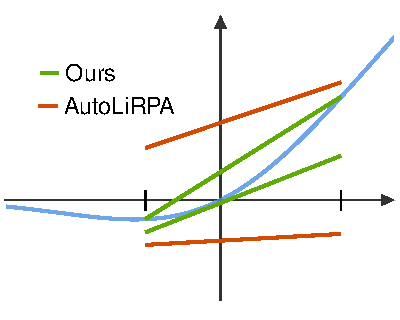
\includegraphics[width=0.8\linewidth]{onlinesyn/figs/ours_vs_autolirpa.pdf}
%	\caption{Linear bounds for $ gelu(x) $.\label{onlinesyn:fig:boundcompare}}
%	\vspace{-2ex}
%\end{wrapfigure}

Our method differs from these existing frameworks because a user (usually an
expert in neural network verification) must provide
hand-crafted, sound linear bounds for the activation functions of a
neural network.
%
%However, to date, they only supports common activations
%like ReLU, sigmoid, tanh, and the exp function, and binary operations,
%namely addition, subtraction, multiplication, and division.
%
However, to date, they only support the previously mentioned activation
functions. We note however that the recent framework~\autolipra{} supports
binary operations (namely addition, subtraction, multiplication, and division)
as ``activation functions''. Thus, while it's not explicitly designed to handle
complex
activations, it has the ability to by decomposing, e.g., $ gelu(x) $ into
operations that it supports, and then combining them. In contrast,~\Name{}
bounds the activation function \textit{as a whole}, which we will show produces
much tighter linear bounds.
%
%Specifically, for $ \mathit{gelu}(x) $, it could first decompose $ x + x^3 $
%into $ x + x
%\times x \times x $, then bound $ x \times x $ twice, and then bound an
%addition with $ x $. It would then bound a multiplication, a $ tanh $, an
%addition, and finally two more multiplications.
%%
%We illustrate the effect of such decomposition in
%Fig.~\ref{onlinesyn:fig:boundcompare}
%by
%showing the linear bounds computed by this approach vs.~\Name{}, which does not
%perform decomposition. We can see~\Name{}'s bounds are significantly tighter
%while being fully automatic.

%While decomposing makes these frameworks applicable to a wide
%variety of network architectures and activation functions, decomposing loses
%any tightness guarantees for the activation function as a whole, and we show
%experimentally that it drastically reduces the precision of the analysis.
%This decomposition loses any tightness guarantees for $ \sigma $ as a whole,
%leading to looser bounds, and significantly reducing the precision of the
%analysis.

% lacks support for several operations and activations
% decomposing loses any guarantees on tightness




%\subsubsection{\textcolor{red}{Does it work in practice?}}

We have implemented our method in tool called \Name{}, and evaluated it on
benchmarks in computer vision and natural language processing (NLP).
Our evaluation shows that we can obtain final output bounds often 2-5X
tighter than the most general tool~\cite{autolipra}, thus allowing us to drastically
increase certified robustness.
%
In addition, our tool achieves accuracy equal to or better
than the handcrafted LSTM bounds of \Popqorn{}~\cite{ko2019popqorn}, which is
currently the most accurate tool for analyzing LSTM-based NLP models, at a
comparable runtime.



%\subsubsection{\textcolor{red}{List of the innovative claims}}

To summarize, this paper makes the following contributions:
\begin{itemize}
	\item We propose the first method for automatically synthesizing  tight linear bounds for
	arbitrary activation functions.
	\item We implement our approach in a tool called~\Name{}, and integrate it
	as a bounding module into the~\autolipra{} framework, thus producing a
	neural network verification tool that can theoretically compute tight linear
	bounds for any arbitrary activation function.
	\item We extensively evaluate our approach and show it outperforms
	state-of-the-art tools in terms of accuracy and certified robustness by a
	large margin.
\end{itemize}


The rest of this chapter is organized as follows.  First, we provide the
technical background in Section~\ref{onlinesyn:sec:preliminaries}.  Then, we
present our method for synthesizing the linear bounds in
Section~\ref{onlinesyn:sec:method-1} and our method for verifying the linear
bounds in Section~\ref{onlinesyn:sec:method-2}.  Next, we present the
experimental results in Section~\ref{onlinesyn:sec:experiment}. Finally, we
summarize the contributions of this chapter in
Section~\ref{onlinesyn:sec:conclusion}.



\section{Preliminaries}
\label{onlinesyn:sec:preliminaries}

In this section, we define the neural network verification problem, and
illustrate both how state-of-the-art verification techniques work, and their
limitations.

\subsection{Neural Networks}

%\subsubsection{introduce the canonical problem: given an input region, compute
%	an over-approximation of the output region}
%\subsubsection{this problem formulation allows us to verify all sorts of good
%	properties like robustness to L-norm perturbations}

Following conventional notation, we refer to matrices with capital bold letters
(e.g. $ \mathbf{W} \in \mathbb{R}^{n \times m}$), vectors as lower case bold
letters (e.g. $ \mathbf{x} \in \mathbb{R}^n $), and scalars or variables with
lower case letters (e.g. $ x \in \mathbb{R} $). Slightly deviating from the
convention, we refer to a set of elements with capital letters (e.g. $ X
\subseteq \mathbb{R}^n $).

We consider two types of networks in our work: feed-forward and recurrent. We
consider a feed-forward neural network to be a (highly) non-linear function $f :
\mathbb{X} \to \mathbb{Y} $, where $\mathbb{X} \subseteq \mathbb{R}^n$ and $
\mathbb{Y} \subseteq \mathbb{R}^m $. We focus on neural network
\textit{classifiers}. For an input $ \mathbf{x} \in \mathbb{X} $, each element
in the output $ f(\mathbf{x}) $ represents a score for a particular class, and
the class
associated with the largest element is the chosen class. For example, in image
classification, $ \mathbb{X} $ would be the set of all images, each element of
an input $ \mathbf{x} \in \mathbb{X} $ represents a pixel's value, and each
element in $ \mathbb{Y} $ is associated with a particular object that the image
might contain.
%We refer to each element (or dimension) of $ \mathbb{X} $ with
%the variables $ x_1, ..., x_n $, and each element of $ \mathbb{Y} $ with $
%y_1,
%..., y_m $.


In feed-forward neural networks the output $ f(\mathbf{x}) $ is computed by
performing a
series of affine transformations, i.e., multiplying by a weight matrix, followed
by application of an activation function $ \sigma(\cdot) $. Formally, a neural
network with $ l $ layers has $ l $ two-dimensional weight matrices and $ l $
one-dimensional bias vectors $ \mathbf{W_i}, \mathbf{b_i},$ where $i
\in {1..l}
$, and thus we have $ f(\mathbf{x}) = \mathbf{W_l} \cdot \sigma(\mathbf{W_{l-1}}
\dots \cdot \sigma(\mathbf{W_1} \cdot \mathbf{x} + \mathbf{b_1}) \dots +
\mathbf{b_{l-1}}) + \mathbf{b_l} $, where $ \sigma(
\cdot ) $
is the activation function applied element-wise
to the input vector. The default choice of activation is typically the
sigmoid $ \sigma(x) = 1 / (1 + e^{-x}) $, $ \tanh{} $, or ReLU
function $\sigma(x) = max(0, x) $, however recent
work~\cite{hendrycks2016gaussian,ramachandran2017searching,radford2018improving}
 has shown that functions such as $ gelu(x) $ and $ \mathit{swish}(x) = x
\times \mathit{sigmoid}(x) $ can have better performance and desirable
theoretical properties.

Unlike feed-forward neural networks, recurrent neural networks receive a
sequence of inputs $ [\mathbf{x^{(1)}}, $  $ \dots, $  $ \mathbf{x^{(t)}} ] $, and
the
final
output of $ f $ on $ \mathbf{x_t} $ is used to perform the classification of
the whole sequence. Recurrent neural networks are
\textit{state-ful}, meaning they maintain a state vector
that contains information about inputs previously given to
$ f $, which also gets updated on each call to $ f $.
%
In particular, we focus on \textit{long short-term memory} (LSTM) networks, which
have seen wide adoption in natural language processing (NLP) tasks due to their
sequential nature. For LSTMs trained for NLP tasks, the network receives a
sequence of \textit{word embeddings}. A word embedding is an $ n $-dimensional
vector that is associated with a particular word in a (natural) language. The
distance between word embeddings carries semantic significance -- two word
embeddings that are close to each other in $ \mathbb{R}^n $ typically have
similar meanings or carry a semantic relatedness (e.g. \textit{dog} and
\textit{cat} or \textit{king} and \textit{queen}), whereas unrelated words
typically are farther apart.

LSTM networks further differ from feed-forward networks in
that their internal activation functions are \textit{two}-dimensional.
Specifically, we have the following two activation patterns: $ \sigma_1(x)
\times \sigma_2(y) $ and $ x \times \sigma_1(y) $. The default choices are $
\sigma_1(x) = sigmoid(x) $, and $ \sigma_2(x) = tanh(x) $. However, we can swap
$ \sigma_1 $ with any function with output range bounded by $ [0, 1] $, and
swap $ \sigma_2 $ with any function with output range bounded by $ [-1, 1] $.
Indeed, prior work~\cite{gomes2008complementary} has shown that $ \sigma_1(x) =
1 - e^{e^{-x}} $ can achieve better results in some applications.

%We focus on \textit{long-term
%short-term}  (LSTM) recurrent neural networks, which maintain two state
%vectors, namely a hidden state $ \mathbf{h} $ and a cell state $ \mathbf{c} $.
%A (1-layer) LSTM has four weight matrices and bias vectors $ \mathbf{W_i},
%\mathbf{b_i}, i \in \{1..5\} $. Given the current input $ \mathbf{x_j} $,
%current cell state and hidden state $ \mathbf{c_{j-1}}, \mathbf{h_{j-1}} $, we
%compute the next state vectors $ \mathbf{c_j}, \mathbf{h_j} $ and output $
%f(\mathbf{x_j}) $ as follows:


% keep a hidden state vector based on previous inputs
% typically, used in NLP, so the inputs are word embeddings
% 	- word embeddings are an n-dimensional vector assigned to words, typically
% words that are related will be closer to each other
%

\subsection{Neural Network Verification}

%\begin{figure}[h]
%	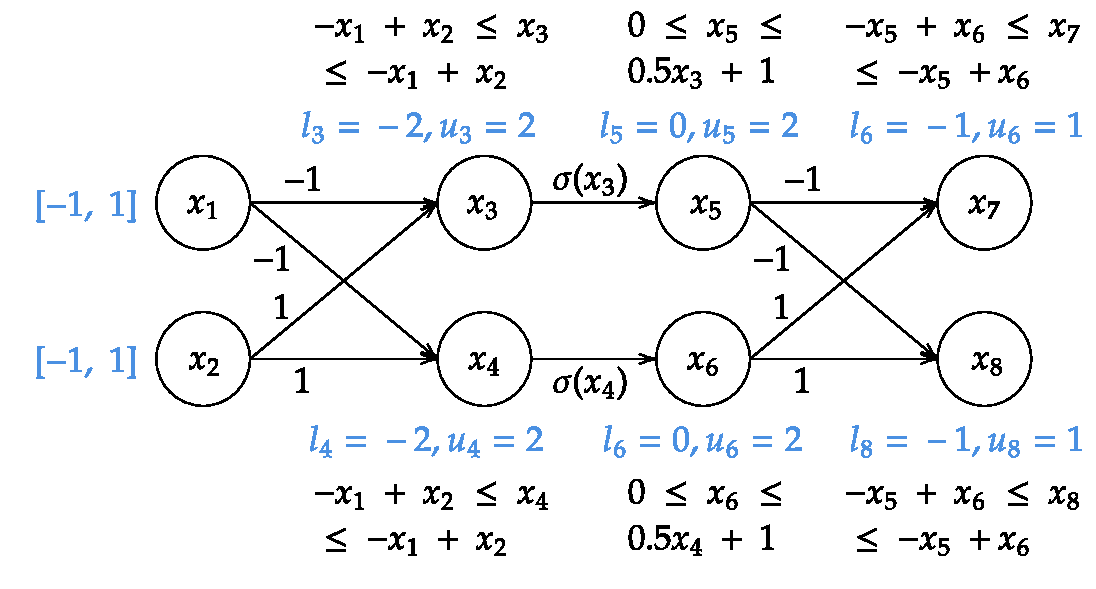
\includegraphics[width=0.6\linewidth]{onlinesyn/figs/motex.pdf}
%	\caption{Neural network verification example. \label{onlinesyn:fig:motex}}
%\end{figure}

%A common verification problem for neural networks is to prove that a point $
%x_0 \in \mathbb{X} $ is \textit{robust}, i.e. making small perturbations to $
%x_0 $ does not change the classification. The set of all small perturbations
%is
%represented by an $ l_p $ ball with radius $ \epsilon $ and center $ x_0 $. We
%focus on $ p = \infty $, though core technique of our approach and others
%extends to other $ p $.

A large number of problems in neural network verification can be phrased as the
following:
%The most common verification problem for neural networks is to prove that a
%region of the input space always maps to the correct class.
%Formally,
given an input region $ X \subseteq \mathbb{X} $, compute an
over-approximation $ Y $, such that $ \{ f(\mathbf{x})\;  | \; \mathbf{x} \in X
\} \subseteq Y \subseteq \mathbb{Y} $. Typically $ X $ and $ Y
$ are hyper-boxes represented by an interval for each of their elements.
A common problem is to prove that a point $ \mathbf{x} \in
\mathbb{X} $ is \textit{robust}, meaning that small perturbations will not
cause an incorrect classification. In this case, $ X $
is the set of all perturbed versions of $ \mathbf{x} $, and
to prove robustness, we check that the element of the correct class in $ Y $
has a lower bound that is greater than the upper bound of all other elements.

%Then, given an input region $ X \subseteq \mathbb{X} $, the standard
%verification problem is to compute an over-approximation $ Y $, such that $ \{
%f(x)\;  | \; x \in X \} \subseteq Y \subseteq \mathbb{Y} $. We can then
%analyze
%the region $ Y $ and potentially prove, for example, that the classification
%is
%always the same for all $ x \in X $. In the literature, $ X $ is often an $
%l_\infty $ ball of radius $ \epsilon $ with center point $ x_0 \in \mathbb{X}
%$. For example, $ x_0 $ may be an image, the $ l_\infty $ ball around this
%point represents all possible small perturbations to the image, and computing
%$
%Y $ may allow us to prove that the classification of $ x_0 $ is robust to all
%small perturbations.

We illustrate a simple verification problem on the neural network shown in
Fig.~\ref{onlinesyn:fig:motex}. The network has two inputs, $ x_1, x_2 $, and two
outputs
$ x_7, x_8 $ which represent scores for two different classes. We refer to the
remaining hidden neurons as $ x_i, i \in {3..6} $. Following prior
work~\cite{SinghGPV19}, we break the affine transformation and application of
the activation function into two separate neurons, and the neurons are assumed
to be ordered such that, if $ x_i $ is in a layer before $ x_j $, then $ i < j
$.
For simplicity, in this motivating example, we let $ \sigma(x) = max(0, x) $ (the ReLU function).
We are interested in proving that the region $ x_1 \in [-1, 1], x_2 \in [-1 ,1]
$ always maps to the first class, or in other words, we want to show that the
lower bound of $ x_7 $ is greater than the upper bound $ x_8 $.

\begin{figure}[t]
	\centering
	\begin{minipage}{.63\textwidth}
		\centering
		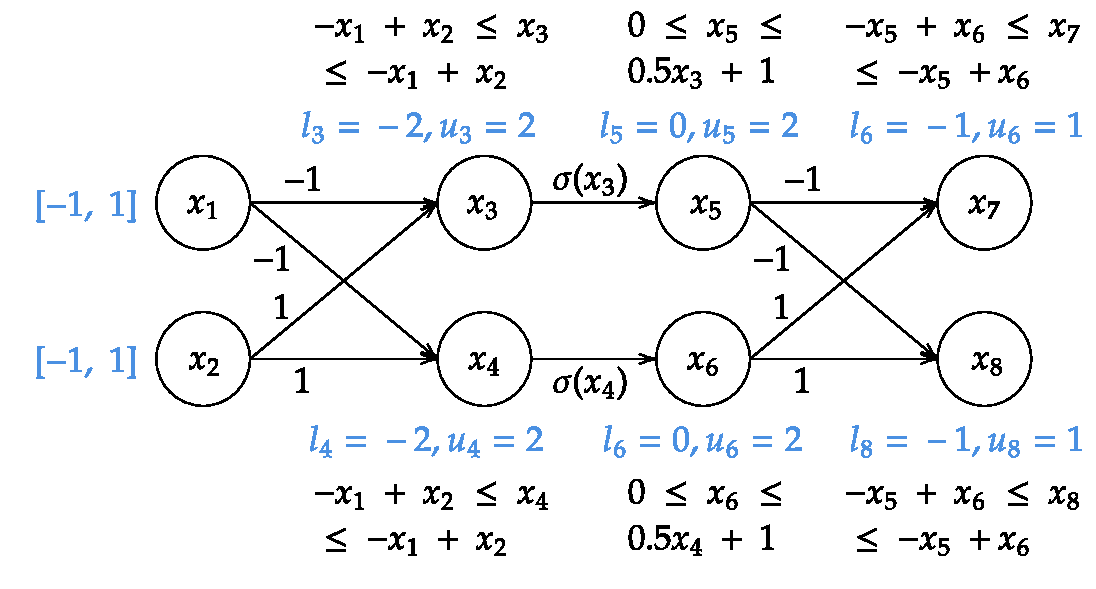
\includegraphics[width=\linewidth]{onlinesyn/figs/motex.pdf}
		%		\captionof{figure}{A figure}
		\caption{Example of neural network verification.}
		\label{onlinesyn:fig:motex}
	\end{minipage}\hspace{24pt}%
	\begin{minipage}{.27\textwidth}
		\centering
		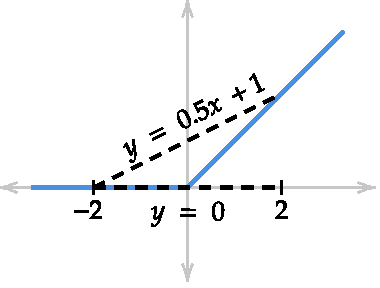
\includegraphics[width=\linewidth]{onlinesyn/figs/relu_relax.pdf}
		%		\captionof{figure}{Another figure}
		\caption{Linear bounds for ReLU activation.}
		\label{onlinesyn:fig:linearbound}
	\end{minipage}
\end{figure}


\subsection{Existing Methods}

%\subsubsection{SOTA is based on linear bounding and back-substitution,
%sometimes referred to as polyhedral constraints, or symbolic intervals}
% TODO: add references to
The most scalable approaches (to date) for neural network verification are
based on linear bounding and back-substitution~\cite{autolipra}, also referred
to
as abstract interpretation in the polyhedral abstract domain~\cite{SinghGPV19} or symbolic
interval analysis~\cite{WangPWYJ18nips} in prior work.


For each
neuron $ x_j $ in the network, these approaches compute a concrete lower and
upper bound $ l_j, u_j $, and a linear lower and upper bound in terms of the
previous layer's neurons. The linear bounds (regardless of the choice of $
\sigma(\cdot) $) have the following form:
$ \sum_{i=0}^{j-1} x_i \cdot c^l_i + c^l_j \leq x_j \leq \sum_{i=0}^{j-1}
x_i \cdot c^u_i + c^u_j $. The bounds are computed in a forward, layer-by-layer
fashion which guarantees that any referenced neurons will already have a bound
computed when back-substitution is performed.


To obtain the concrete bounds $ l_j, u_j $ for a neuron $ x_j $, the bounds of
any non-input neurons are recursively substituted into the linear bounds of $
x_j $ until only input nodes $ x_1, ..., x_n $ remain. Finally, the concrete
input intervals are substituted into the bound to obtain $ l_j, u_j $.


\paragraph{Example}

%\subsubsection{first we multiply by edge weights, then we apply activation
%function}
We illustrate on the two-layer network in Fig.~\ref{onlinesyn:fig:motex} for the
previously defined property. We trivially have $ l_1 = l_2 = -1 $, $ u_1 = u_2
= 1 $, $ -1 \leq x_1 \leq 1 $, and $ -1 \leq x_2 \leq 1 $. We then compute
linear bounds for $ x_3, x_4 $ in terms of previous layer's neurons $ x_1, x_2
$.
We multiply $ x_1, x_2 $ by the edge weights, obtaining $ -x_1 + x_2 $ as the
lower and upper bound for both of $ x_3 $ and $ x_4 $.
Since this bound is already in terms of the input variables, we substitute the
concrete bounds into this equation and obtain $ l_3 = l_4 = -2 $ and $ u_3 =
u_4 = 2 $.

Next, we need to compute the linear bounds for $ x_5 = \sigma(x_3) $ and $ x_6
= \sigma(x_4) $ after
applying the activation function. Solving this challenge has been the focus of
many prior works. There are two requirements. First, they need to be
\textit{sound}. For example, for $ x_5 $ we need to find coefficients $
c_1^l,c_2^l,c_1^u,c_2^u $ such that
$c_1^l x_3 + c_2^l
\leq \sigma(x_3) \leq c_1^ux_3 + c_2^u $ for all $x_3 \in [l_3, u_3]$, and similarly for $ x_6 $. Second, we
want them to be \textit{tight}. Generally, this means that volume below the
upper bound is minimized, and volume below the lower bound is maximized.


As an example, prior work~\cite{SinghGPV19,zhang2018efficient} has proposed the
following
sound and 	tight bound for $ \sigma(x) $  $ = $  $ max(0, x) $:
\[
	\forall x_i \in [l_i, u_i] ~.~ \frac{u_i}{u_i - l_i}x_i +
	\frac{-l_iu_i}{u_i-l_i} \leq \sigma(x_i)
	\leq \begin{cases}
	0 & -l_i \geq u_i\\
	x_i & -l_i < u_i
	\end{cases}
\]
We illustrate the bound for $ x_5 $ in Fig.~\ref{onlinesyn:fig:linearbound}. After
computing this bound, we recursively substitute variables in the
bounds of $ x_5 $ with the appropriate bound, and compute $ l_5, u_5 $. The
process then repeats for $ x_6 $, followed by $ x_7 $ and $ x_8 $. We then
check $ l_7 > u_8 $ to verify the property, which fails in this case.


\subsection{Limitations of Existing Methods}

Current approaches only support a limited number of activation functions, and
designing linear bounds for new activation functions often requires a
significant amount of effort even for a domain expert.
%Proving that these bounds are indeed sound also requires a
%domain expert.
%
For example, handcrafted sound and
tight linear
bounds for activation functions such as ReLU, sigmoid, and
tanh~\cite{SinghGPV19,WengZCSHDBD18,zhang2018efficient,wu2021tightening,WangPWYJ18,WangPWYJ18nips},
convolution layers and pooling operations~\cite{boopathy2019cnn}, the
two-dimensional activations found in
LSTMs~\cite{ko2019popqorn,ryou2021scalable}, and those
 in transformer networks~\cite{shi2020robustness} are worthy of publication.
%
Furthermore, even bounds that are hand-crafted by experts are not always
tight. For example, a recent
work~\cite{wu2021tightening} was able to nearly triple the precision
of previous state-of-the-art sigmoid and tanh linear bounds simply by
improving tightness.

%\begin{figure}[t]%% chao: we have plenty of space...
%\begin{wrapfigure}{R}{0.5\textwidth}
%	\centering
%	\vspace{-2ex}
%	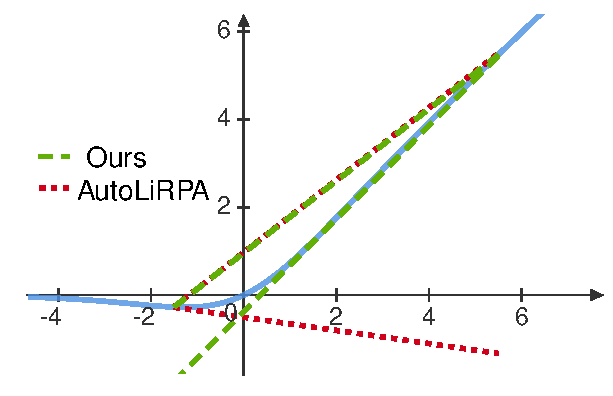
\includegraphics[width=\linewidth]{onlinesyn/figs/ours_vs_autolirpa2.pdf}
%	\caption{Bounds computed by~\Name{} and~\autolipra{} for $ swish(x),
%	x \in [-1.5, 5.5] $.\label{onlinesyn:fig:boundcompare2}}
%	\vspace{-2ex}
%\end{wrapfigure}
%\end{figure}

To the best of our knowledge,~\autolipra{}~\cite{autolipra} is the only tool
that has the ability to handle more complex activation functions, though it was
not originally designed for this. It
can do so by decomposing them into simpler
operations, and then composing the bounds together. We illustrate with $
swish(x) = x \times sigmoid(x) $, where $ x \in [-1.5, 5.5] $.~\autolipra{}
would first bound $ sigmoid(x) $ over the region $ [-1.5, 5.5] $, resulting in
the bound $ .11x + .35 \leq sigmoid(x) \leq .22x + .51 $.
%
For the left-hand side of the function, we
trivially have $ x \leq x \leq x $.
%
~\autolipra{} would then bound a multiplication $ y \times z $, where
in this case $ y = x $ and $ z = sigmoid(x) $, resulting in the final bound
$ -.15x - .495 \leq x\times sigmoid(x) \leq 0.825x + .96 $. We illustrate this
bound in Fig.~\ref{onlinesyn:fig:boundcompare2}, and we provide bounds computed
by~\Name{} as a comparison point.~\Name{} provides a slightly better upper
bound, and a significantly better lower bound. The reason for the looseness is
because when~\autolipra{} bounds $ sigmoid(x) $, it necessarily accumulates some
approximation error because it is approximating the behavior of a non-linear
function with linear bounds. The approximation error effectively ``loses some
information'' about about its input variable $ x $. Then, when bounding the
multiplication operation, it has partially lost the information that $ y $ and
$ z $ are related (i.e. they are both derived from $ x $).
%
In
contrast,~\Name{} overcomes this issue by considering $ swish(x) $ as a whole.
We explain how in the following sections.
%\textcolor{red}{Please  explain
%%
%(1) how  AutoLiPRA works, and
%%
%(2) why its linear bounding technique can be less accurate.
%%
%It might be good to use \texttt{Swish} as an example.
%%
%Use it to show why AutoLiPRA does not work well (error adds up significantly
%during composition),
%%
%and then give the reason why our method is better (computing bounds for the
%entire function in one shot, thus reducing the error)}



%\subsubsection{Require hand-crafted bounds: requires an expert to prove sound,
%and may not be tight}

\section{Synthesizing the Candidate Linear Bounds}
\label{onlinesyn:sec:method-1}

In this section, we describe our method for synthesizing candidate, possibly
unsound linear bounds.

\subsection{Problem Statement and Challenges}

%\highlight{What are the inputs (given the activation function $\sigma()$ and
%the input region)?}

We assume we are given a $ d $-dimensional activation function $ z =
\sigma(x_1,...,x_d) $, and an input interval $ x_i \in [l_i, u_i] $ for each $ i
\in \{1..d\} $. Our goal is to synthesize linear coefficients $ c^l_i, c^u_i$, where $i
\in \{1..d+1\} $ that are sound, meaning that the following condition holds:
\begin{equation} \label{onlinesyn:eq:generalsound}
\begin{gathered}
\forall x_1 \in [l_1, u_1], x_2 \in [l_2, u_2], \dots, x_d \in [l_d, u_d]\\
c^l_1x_1 + c^l_2x_2 + \dots + c^l_{d+1}
\leq \sigma(x_1, x_2, \dots) \leq
c^u_1x_1 + c^u_2x_2 + \dots + c^u_{d+1}
\end{gathered}
\end{equation}

In addition, we want to ensure that the bounds are \textit{tight}. The ideal
definition of tightness would choose linear bounds that maximize the precision
of the overall analysis, for example minimizing the width of the output
neuron's intervals.
%
Unfortunately, such a measure would involve all of the neurons of the network,
and so is impractical to compute.
Instead, the common practice is to settle for tightness that's local to the specific neuron we are
bounding.

\begin{figure}[t]%% chao: we have plenty of space...
	\centering
	\begin{minipage}{0.48\textwidth}
		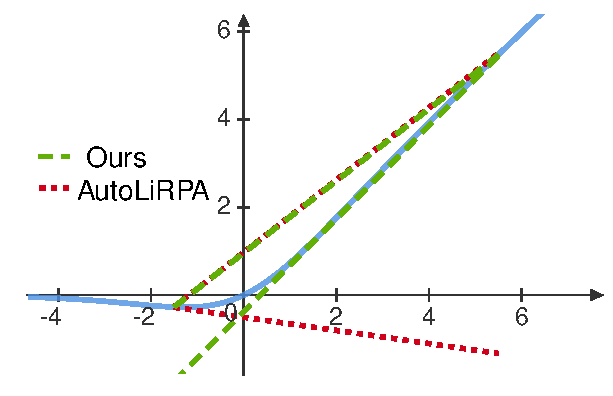
\includegraphics[width=0.9\linewidth]{onlinesyn/figs/ours_vs_autolirpa2.pdf}
		\caption{Bounds computed by~\Name{} and~\autolipra{} for $ swish(x)$, $
			x \in [-1.5, 5.5] $.\label{onlinesyn:fig:boundcompare2}}
	\end{minipage}%
	\begin{minipage}{0.48\textwidth}
		\centering
		\scalebox{1.0}{
			\begin{tikzpicture}
    \begin{axis}[
        height = .85\textwidth,
        width = \textwidth,
        axis on top = true,
        axis x line = bottom,
        axis y line = left,
        x axis line style = -,
        y axis line style = -,
        tick align = outside,
        every tick/.append style = {
            black,
            thin,
            font=\tiny
        },
%       grid = major,
        ymin = 0,
        ymax = 1.1,
		xmin=-5,
		xmax=5,
        xlabel = $x_1$,
%        ylabel = $ z $
    ]
    % sigmoid function
        \addplot[
            blue,
            domain = -5:5,
            samples = 100,
			postaction={
        decoration={
          markings,
          mark=between positions 0.38 and .9 step 0.15
               with { \fill circle[radius=1.5pt]; },
        },
        decorate,
      },
        ]
            {1/(1+exp(-x))};

		% upper bound line
       \addplot[
			name path=f,
            dkgreen,
            domain = -1:3.5,
            samples = 200,
        ]
            {0.649906 + 0.104561*x};

		%min shift text
			\node[label={{\textcolor{red}{min shift}}},inner sep=1pt] (source)
			at (axis cs:0.5,.9) {};

		       \node (destination) at (axis
		       cs:2.005,0.881321){};

		% arrow pointing to min shift line
		\draw[->,>=stealth,red](source.south) to [out=270,in=180] (destination);
%        \draw[->](source.south)--(destination);
	    \addplot[
					thick,
            red,
            domain = 2.005:2.08,
            samples = 200,
        ]
            {0.881321 + -(0.02/0.104561)*(x - 2.005)};


		\path[name path=axis] (axis cs:-1,0) -- (axis cs:3.5,0);
		\addplot [
        thick,
        color=blue,
        fill=blue,
        fill opacity=0.05
    ]
	fill between[
        of=f and axis,
        soft clip={domain=-1:3.5},
    ];

		\node at (axis cs:2.0,0.2)
		{$\displaystyle\int_{-1}^{3.5} c_1^ux_1 +
		c_2^u \, dx$};
    \end{axis}
\end{tikzpicture}
		}
		\caption{Candidate plane synthesis.\label{onlinesyn:fig:running_example}}
	\end{minipage}
\end{figure}
Informally, we say a bound is \textit{tight} if the volume below the
upper bound is minimized, and volume below the lower bound is maximized.
%
Prior work~\cite{zhang2018efficient,SinghGPV19,ko2019popqorn} has
found this to be a good heuristic\footnote{We also experimented with minimizing
the volume between the linear bound and the activation function, which gave
almost identical results.}.
%\footnote{Minimizing the volume below
%the upper bound is computationally cheaper, and yet has the effect
%of \emph{indirectly} minimizing the region between the upper bound and
%the activation function, since the volume below the activation
%function is fixed.}.
%
%Formally, the tightness objective for the coefficients of the
%upper bound is:
Formally, volume is defined as the following integral:
%\begin{equation}
$
\int_{l_1}^{u_1} \dots \int_{l_d}^{u_d} \sum_{i=1}^{d}
c^u_ix_i + c^u_{d+1} \; dx_1 \dots dx_d
$
%\end{equation}
which, for the upper bound, should be minimized subject to
Equation~\ref{onlinesyn:eq:generalsound}. This
integral has the following closed-form solution:
\begin{equation} \label{onlinesyn:eq:vol}
\sum_{i=0}^{d} \left[
\frac{1}{2}c_i \times \prod_{j=0}^{d}
\left(
u_i^{1 + \mathbf{1}_{i=j}} - l_i^{1 + \mathbf{1}_{i=j}}
\right)
\right] +
c_{d+1} * \prod_{i=0}^d (u_i - l_i)
\end{equation}
where $ \mathbf{1}_{i=j} $ is the (pseudo Boolean) indicator function that
returns $ 1 $ when its predicate is true.
%
We omit the proof, but note that the above expression can be
derived inductively on $ d $. Also note that, since each $ l_i, u_i $ are
concrete, the above expression is linear in terms of the coefficients, which
will be advantageous in our approach below.

While recent approaches in solving non-linear optimization
problems~\cite{kong2018delta,chabert2009contractor} could directly minimize
Equation~\ref{onlinesyn:eq:vol}
subject to Equation~\ref{onlinesyn:eq:generalsound} in one step, we find the
runtime to
be very slow. Instead, we adopt a two-step approach that
first uses efficient procedures for computing candidate coefficients that are
almost sound (explained in this section), and second, only calls an SMT
solver when necessary to verify Equation~\ref{onlinesyn:eq:generalsound}
(explained in
the next
section).
%In the first step, we compute candidates for the coefficients $ c^l_i, c^u_i $
%by using an efficient sampling based approach. We design this procedure  Since
%these coefficients are generally not sound, we add a second step we estimate a
%\textit{shift} to be added to the bound as a best-effort to make it sound.
%Finally, we add the shift to the bound, and use an SMT solver to verify
%it's soundness, further adjusting if necessary.
We illustrate the approach on a concrete example.


\subsection{Synthesizing Candidate Bounds}

The first step in our approach computes candidate coefficients for the linear
bound. In this step we focus on satisfying the tightness requirement, while
making a best effort for soundness. We draw inspiration from prior
work~\cite{ryou2021scalable,balunovic2019certifying} that leverages sampling to
estimate the curvature of a particular function, and then uses a linear
programming (LP) solver to compute a plane that is sound. However, unlike prior
work which targeted a fixed function, we target arbitrary (activation)
functions, and thus these are special cases of our approach.

%Since the volume is our objective function, we hand-derive the solution to the
%integral in Equation~\ref{onlinesyn:eq:synth}:
%\begin{equation} \label{onlinesyn:eq:vol}
%	\sum_{i=0}^{d} \left[
%		\frac{1}{2}c_i \times \prod_{j=0}^{d}
%		\left(
%			u_i^{1 + \\mathds{1}_{i=j}} - l_i^{1 + \\mathds{1}_{i=j}}
%		\right)
%	\right] +
%	c_{d+1} * \prod_{i=0}^d (u_i - l_i)
%\end{equation}
%where $ \\mathds{1}_{i=j} $ is the (pseudo Boolean) indicator function that
%returns $ 1 $ when
%its predicate is true. We omit the proof, but note that the above expression
%can be
%derived inductively on $ d $. Also note that the above expression is linear in
%terms of the
%coefficients, which are the variables in the linear program, and thus can be
%directly used as the objective for the LP solver.


The constraints of the LP are
determined by a set of sample points $ S \subset \mathbb{R}^d $. For the upper
bound, we
minimize Equation~\ref{onlinesyn:eq:vol}, subject to the constraint that the
linear bound
is above $ \sigma(\cdot) $ at the points in $ S $. Using $ \mathbf{s}_i $ to
refer to the $ i^{th} $ element of the vector $ \mathbf{s} \in S $, the linear
program we solve is:
\begin{equation}\label{onlinesyn:eq:lp}
\begin{gathered}
	\text{minimize}\;\text{Equation}\;(\ref{onlinesyn:eq:vol}) ~~
	\text{subject to} \bigwedge_{\mathbf{s} \in S} c_1\mathbf{s}_1 +
	c_2\mathbf{s}_2  + \dots + c_{d+1} \geq \sigma(\mathbf{s})
\end{gathered}
\end{equation}
We generate $ S $ by sampling uniformly-spaced points over the input intervals.


\paragraph{Example}

We demonstrate our approach on the running example illustrated in
Fig.~\ref{onlinesyn:fig:running_example}. For the example, let
$ \sigma(x_1) = \frac{1}{1 + e^{-x_1}} $ (the sigmoid function, shown as the
blue curve), where $ x_1 \in [-1, 3.5] $. We focus only on the upper bound, but
the lower bound is computed analogously.


Plugging in the variables into
Equation~\ref{onlinesyn:eq:vol}, the objective of the LP that we minimize is:
%\begin{equation}
$
\displaystyle\int_{-1}^{3.5} c_1^ux_1 + c_2^u \,dx_1 = 6.625c_1^u + 4.5c_2^u
$
%\end{equation}
which is shown as the shaded region in Fig.~\ref{onlinesyn:fig:running_example}.

We
sample the points  $ S = \{-1, 0.25, 1.5, 2.75\} $, resulting in the following
four constraints:
$ -c_1 + c_2 \geq \sigma(-1) \wedge 0.25c_1 + c_2 \geq \sigma(0.25) \wedge
1.5c_1 + c_s \geq \sigma(1.5) \wedge 2.75c_1 + c_2 \geq \sigma(2.75) $.	Solving
the LP program results in $ c_1 = 0.104, c_2 = 0.649 $, which is illustrated by the
green line in Fig.~\ref{onlinesyn:fig:running_example}.


%Solving Equation~\ref{onlinesyn:eq:lp} typically produces good estimates for the
%coefficients of the bound, however most often the overall bound will not be
%sound.

%We first define the violation of the upper bound as:
%\begin{equation}
%	v(x_1, x_2,\dots) := c^u_1x_1 + c^u_2x_2 + \dots + c^u_{d+1} + shift -
%\sigma(x_1, x_2, \dots)
%\end{equation}


%We make the bound sound by computing a \textit{minimum shift}, that
%adjusts the bound upward (resp. downward for the lower bound) to make it sound.
%The minimum shift is illustrated by the red line in
%Fig.~\ref{onlinesyn:fig:running_example}. Formally, this shift is:
%\begin{equation}
%	\text{shift} = \text{minimize } c_1x_2 + c_2x_2 + \dots + c_{d+1} -
%	\sigma(x_1, x_2, \dots)
%\end{equation}
%Since failed calls to the SMT solver can be expensive, we first estimate
%a \textit{minimum shift} to make the plane sound.

% sampling
% the volume forumla

%\subsubsection{how to do it}



%\subsubsection{Running Example}

%We demonstrate our approach for synthesizing an upper bound on an example
%where $ \sigma(x) = \frac{1}{1 + e^{-x}} $ (the sigmoid function), where $ x
%\in [-1, 3.5] $. Our goal is then is to synthesize coefficients $ c_1^u, c_2^u
%$
%such that the following holds:
%\begin{equation} \label{onlinesyn:eq:sound_motex}
%\begin{gathered}
%	\forall x_1 \in [l_1, u_1]. \; \sigma(x_1) \leq c_1^ux_1 + c_2^u
%\end{gathered}
%\end{equation}




%\subsection{Computing the Candidate Coefficients}
%The first step is to compute candidate coefficients $ c_1^u, c_2^u $ that
%minimize/maximize some objective function. In our work, the objective function
%is to minimize the volume below the bound. This volume is illustrated by the
%shaded region in Fig.~\ref{onlinesyn:fig:cand_syn}, and the formal definition of
%the
%volume is shown by the integral. We note that, when the integral is evaluated,
%it results in a \textit{linear} equation in terms of $ c_1^u, c_2^u $, and
%hence can be efficiently minimized by an LP solver. Specifically, we have:
%\begin{equation}
%\displaystyle\int_{-1}^{3.5} c_1^ux + c_2^u \,dx = 6.625c_1^u + 4.5c_2^u
%\end{equation}
%
%Additionally, we need to encode the constraint that
%\begin{gather*}
%\forall x_1 \in [l_1, u_1].\; \sigma(x_1) \leq c_1^ux_1 + c_2^u
%\end{gather*}
%Since $ \sigma(x_1) $ is non-linear, we cannot directly encode this constraint
%for an LP-solver. Instead, we estimate the curve of $ \sigma $ by uniformly
%sampling many points on it over $ x_1 \in [-1, 3.5] $, as shown by the dots
%in Fig.~\ref{onlinesyn:fig:cand_syn}, and then encoding the constraint that $
%c_1^ux_1
%+  c_2^u $ should be greater than all of these points. Formally, given $ n $
%sample points $ \{(s_1, \sigma(s_1)), ..., (s_n, \sigma(s_n))\} $, the
%constraint we make is:
%\begin{equation} \label{onlinesyn:eq:sample_constr}
%	\bigwedge_{i \in \{1..n\}} \sigma(s_i) \leq c_1^us_i + c_2^u
%\end{equation}
%Finally, we use an LP solver to minimize Equation~\ref{onlinesyn:eq:vol} subject
%to the
%constraint in~\ref{onlinesyn:eq:sample_constr}.

%\subsection{Estimating the Shift}
%The result of the first step is candidate values for $ c_1^u, c_2^u $. These
%coefficients may not be sound, i.e. Equation~\ref{onlinesyn:eq:sound} does not
%hold,
%since the sampled points do not fully capture the curvature of $ \sigma $. In
%order to make it sound, we need to compute an (upward) shift to make
%Equation~\ref{onlinesyn:eq:sound} hold. Formally, the smallest shift is:
%\[
%\mathrm{shift} = \min \; c_1^ux_1 + c_2^u  - \sigma(x_1)
%\]
%We estimate this minimum using the L-BFGS-B~\cite{byrd1995limited} local
%optimization procedure, which typically produces a minimum value within $
%10^{-8} $ of the true minimum. This quantity is illustrated by the small red
%line in Fig.~\ref{onlinesyn:fig:cand_syn}. We add the value of $ \mathrm{shift} $
%plus
%a small tolerance ($ 10^{-7} $) to $ c_2^u $.

\section{Making the Bound Sound}
\label{onlinesyn:sec:method-2}

In this section, we present our method for obtaining soundness because the
candidate bounds synthesized in the previous section may not be
sound. Here, we focus only on making the upper bound sound, but note the
procedure for the lower bound is similar.

\subsection{Problem Statement and Challenges}
We are given the activation function $ \sigma(\cdot) $, the input intervals $
x_i \in [l_i, u_i] $, and the candidate coefficients $ c_1, c_2,
\dots,c_{d+1} $. The goal is to compute an upward shift, if needed, to make the upper bound sound. First,
we define the violation of the upper bound as:
\begin{equation}
	v(x_1, x_2,\dots,x_d) := c^u_1x_1 + c^u_2x_2 + \dots + c^u_{d+1} -
	\sigma(x_1, x_2, \dots,x_d)
\end{equation}
A negative value indicates the upper bound is not sound. We then need to compute a
lower bound on $ v(\cdot) $, which we term $ v_l $. Then the equation we pass
to the verifier is:
\begin{equation} \label{onlinesyn:eq:makesound}
\begin{gathered}
\forall x_1 \in [l_1, u_1], x_2 \in [l_2, u_2], \dots, x_d\in[l_d, u_d]\\
v(x_1, x_2, \dots, x_d) + (-v_l) \geq 0
\end{gathered}
\end{equation}
Expanding $ v(\cdot) $ with its definition in the above equation results in the
soundness definition of Equation~\ref{onlinesyn:eq:generalsound}. Thus, if the
verifier
proves Equation~\ref{onlinesyn:eq:makesound}, then shifting the upper
bound upward by $ -v_l $ ensures its soundness.
%
For our running example, the quantity $ v_l $ is shown by the red line in
Fig.~\ref{onlinesyn:fig:running_example}.


This problem is non-trivial because finding a solution for $ v_l $ requires a
search for a sound global minimum/maximum of a function involving $
\sigma(\cdot) $, which may be highly non-linear.
State-of-the-art  SMT solvers such as  Z3 do not support all non-linear
operations, and furthermore, since we assume arbitrary $ \sigma(\cdot) $, the
problem may even be (computationally) undecidable.
% z3 doesn't support nonlinear theories
% other solvers
% dreal gets slower with

\subsection{Verifying the Bound}
We first assume we have a candidate (possibly unsound) $ v_l $, and explain our
verification method.
To ensure decidability and tractability, we
leverage the \textit{$ \delta $-decision procedure} implemented
by~\dReal{}~\cite{gao2013dreal}. To the best of our knowledge this is is the only
framework that is decidable for all computable functions.

In this context, instead of verifying Equation~\ref{onlinesyn:eq:makesound}, the
formula
is first negated thus changing it into an existentially quantified one, and
then applying a $ \delta $\textit{-relaxation}. Formally, the formula~\dReal{}
attempts to solve is:
\begin{equation} \label{onlinesyn:eq:relaxed_makesound}
\begin{gathered}
\exists x_1 \in [l_1, u_1], x_2 \in [l_2, u_2], \dots, x_d \in [l_d, u_d]\\
v(x_1, x_2, \dots) + (-v_l) \leq \delta
\end{gathered}
\end{equation}
where $ \delta $ is a small constant (e.g. $ 10^{-5} $), which we explain in a
moment. The
above is formulated such that Equation~\ref{onlinesyn:eq:makesound} holds if (but
not
only if) there does \textit{not} exist a solution to
Equation~\ref{onlinesyn:eq:relaxed_makesound}.

Internally,~\dReal{} performs interval constraint propagation (ICP) on the
left-hand
side of Equation~\ref{onlinesyn:eq:relaxed_makesound} over the
intervals defined by each $ [l_i, u_i] $ to compute an upper bound, and
compares this upper bound with $ \delta $. If the upper bound is less than $
\delta $, then no solution exists (i.e.,
Equation~\ref{onlinesyn:eq:relaxed_makesound} is
unsatisfiable, and we have proven the original
Equation~\ref{onlinesyn:eq:makesound} holds). Otherwise
a solution \textit{may} exist. In this case,~\dReal{} iteratively partitions
the input space defined by the $ [l_i, u_i ] $ and repeats this process on
each partition separately.

\dReal{} stops partitioning either when
it proves all partitions do not have solutions
, or when a partition whose intervals all
have width less than some $ \epsilon $ is found. Here, $ \epsilon $ is
proportional to $
\delta $ (i.e., smaller $ \delta $ means smaller $ \epsilon $). In the latter
case,~\dReal{} returns this partition as a ``solution''.


While Equation~\ref{onlinesyn:eq:makesound} holds if there does not exist a
solution to
Equation~\ref{onlinesyn:eq:relaxed_makesound}, the converse does not hold true both
because of the error inherent in ICP, and because
we ``relaxed'' the right-hand side of
Equation~\ref{onlinesyn:eq:relaxed_makesound}.
This means that $ \delta $ controls the
\textit{precision} of the analysis. $ \delta $ controls both the size of the
false solution space, and determines how many times we will sub-divide the
input space before giving up on proving
Equation~\ref{onlinesyn:eq:relaxed_makesound} to
be unsatisfiable.

Practically, this has two implications for our approach. The first one is that our
approach naturally inherits a degree of looseness in the linear bounds defined
by $ \delta $. Specifically, we must shift our plane upward by $
\delta $ in addition to the true $ v_l $, so that~\dReal{} can verify the
bound. The second is that we have to make a trade-off between computation and precision. While
smaller $ \delta $ will allow us to verify a tighter bound, it generally will
also mean a longer verification time.
In our experiments, we find that $ \delta = 10^{-7} $ gives tight bounds at an
acceptable runtime, though we may be able to achieve a shorter  runtime with a
larger $\delta$.

\subsection{Computing $ v_l $}
Now that we have defined how we can verify a candidate bound, we explain our
approach for computing $ v_l $. The implementation is outlined in
Algorithm~\ref{onlinesyn:alg:viol}. Since failed calls to the verifier can be
expensive, at lines 1-2, we first use a relatively cheap (and unsound) local
optimization procedure to estimate the true $ v_l $.
%
While local optimization may get stuck
in local minima, neural network activation functions typically do not have many
local minima, so neither will $ v(\cdot) $.
%
We use L-BFGS-B~\cite{byrd1995limited}, the bounded version of L-BFGS, to
perform the optimization. At a high-level, L-BFGS-B takes as input $ v(\cdot)
$, the input bounds $ x_i \in [l_i, u_i] $, and an initial guess $ \textbf{g}
\in
\mathbb{R}^d $ at the location of the local minimum.
%
It then uses the
Jacobian matrix (i.e., derivatives) of $ v(\cdot) $ to iteratively move towards
the local minimum (the Jacobian can be estimated using the finite differences
method or provided explicitly -- we use Mathematica~\cite{Mathematica} to
obtain it).
%
We find that sampling points uniformly in $ v(\cdot) $ can usually find a good
$ \textbf{g} $, and thus L-BFGS-B often converges in a small number of
iterations.
L-BFGS-B typically produces an estimate within $ 10^{-8} $ of the true value.
%
To account for estimation error we add an additional $ 10^{-6} $, plus $ 2
\times \delta $ to account for the $ \delta $-relaxation (line 3).
%
Finally, we
iteratively decrease $ v_l $ by a small amount ($ 10^{-6} $)
until~\dReal{} verifies it (lines 4-9).


Going back to our motivating example, we would estimate $ v_l $ with a local
minimizer, and then use \dReal{} to verify the following:
\begin{gather*}
\forall x_1 \in [-1, 3.5] ~. \; \sigma(x_1) \leq c_1^ux_1 + c_2^u + (-v_l) + 2
\times \delta + 10^{-6}
\end{gather*}
If verification fails, we iteratively decrease the value of $ v_l $ by $
10^{-6} $, and call \dReal{} until the bound is verified. The final
value of $ c_1^ux_1 + c_2^u + (-v_l) + 2 \times \delta + 10^{-6} $ is the final
sound upper bound.

\subsection{On the Correctness and Generality of~\Name{}}
The full~\Name{} procedure is shown in Algorithm~\ref{onlinesyn:alg:synth}. The
correctness (i.e. soundness) of the synthesized bounds is guaranteed if the $
v_l $ returned by Algorithm~\ref{onlinesyn:alg:viol} is a true lower bound on $
v(\cdot)
$. Since Algorithm~\ref{onlinesyn:alg:viol} does not return until~\dReal{}
verifies $ v_l
$ at line 6, the correctness is guaranteed.
%In addition, the while loop in
%Algorithm~\ref{onlinesyn:alg:viol} is guaranteed to terminate if $ v(\cdot) $ is
%bounded
%over the input space. This will generally be the case if $ \sigma(\cdot) $ is
%bounded, which should always be the case for neural network activation
%functions.

Both our procedure in Section~\ref{onlinesyn:sec:method-1} and L-BFGS-B require
only
black-box access to $ \sigma(\cdot) $, so the only potential limit to the
arbitrariness of our approach lies in what elementary operations are supported
by~\dReal{}. During our investigation, we did not find activations that use
operations unsupported by~\dReal{}, however if an unsupported operation is
encountered, one would only need to define an \textit{interval
extension}~\cite{moore2009introduction} for the operation, which can be done
for any computable function.

\begin{algorithm}[t]
	\SetAlgoLined
	\KwIn{Activation $ \sigma(x_1, x_2, \dots) $, Candidate Coefficients
	$c_1^u, c_2^u, \dots, c_{d+1}^u$, $ ~~~~ $Input Bounds
		$x_1 \in [l_1, u_1], x_2 \in [l_2, u_2],\dots$, Jacobian $\nabla v$
		(optional)}
	\KwOut{Lower Bound on Violation $v_l$}
	$\textbf{g} \gets $ sample points on $v(x_1,x_2,\dots)$ and take minimum\;
	$v_l \gets \textbf{L-BFGS-B}( v(x_1,x_2,\dots),
	x_1 \in [l_1, u_1], x_2 \in [l_2, u_2], \dots, \textbf{g}, \nabla v )$ \;
	$ v_l \gets v_l - 10^{-6} - 2\delta$\;
	\While{$\textbf{True}$}{
		// Call dReal \\
%		\If{$\forall x_1 \in [l_1, u_1], x_2 \in [l_2, u_2], \dots ~.~
%			v(x_1, x_2, \dots) + (-v_l) \geq 0$}
		\If{$ \text{Equation~\ref{onlinesyn:eq:generalsound} holds} $}
		{
			\Return{} $v_l$;
		}
		$v_l \gets v_l - 10^{-6}$;
	}
	\caption{BoundViolation\label{onlinesyn:alg:viol}}
\end{algorithm}
\begin{algorithm}[t]
	\SetAlgoLined
	\KwIn{Activation $\sigma(x_1, x_2, \dots)$, Input Bounds $x_1 \in [l_1,
	u_1],
		x_2 \in [l_2, u_2], \dots$, Jacobian $\nabla v$ (optional)}
	\KwOut{Sound Coefficients $c_1^u, c_2^u, \dots, c_{d+1}^u$}
	$c_1^u, c_2^u, \dots, c_{d+1}^u \gets  \text{Sampling and LP procedure on }
	\sigma(x) \text{ over Input Bounds}$\;
	$v_l \gets \text{BoundViolation}(c_1^u, c_2^u, \dots, c_{d+1}^u, x_1 \in
	[l_1, u_1], x_2 \in [l_2, u_2], \dots, \nabla v)$\;
	$c_{d+1}^u \gets c_{d+1}^u + (-v_l)$\;
	\Return{} $c_1^u, c_2^u, \dots, c_{d+1}^u $\;
	\caption{SynthesizeUpperBoundCoefficients\label{onlinesyn:alg:synth}}
\end{algorithm}

\section{Evaluation}
\label{onlinesyn:sec:experiment}


We have implemented our method in a module called~\Name{}, and
integrated it into the \autolipra{} neural network verification framework~\cite{autolipra}.
A user instantiates \Name{} with a definition of an activation
function, which results in an executable software module capable of
computing the sound linear lower and upper bounds for the activation
function over a given input region.
%
\Name{} uses Gurobi~\cite{gurobi} to solve the LP problem described in
Section~\ref{onlinesyn:sec:method-1}, and \dReal{}~\cite{gao2013dreal} as the
verifier
described in~\ref{onlinesyn:sec:method-2}.
%
In total, \Name{} is implemented in about 1200 lines of Python
code.


\subsection{Benchmarks}

\paragraph{Neural Networks}
Our benchmarks are nine deep neural networks trained on the three
different datasets shown below. In the following, a neuron is a node in the
neural network where a linear bound must be computed, and thus the neuron counts
indicate the number of calls to~\Name{} that must be made.
\begin{itemize}
\item
\textbf{MNIST:}
MNIST is a dataset of hand-written integers labeled with the
corresponding integer in the image. The images have 28x28 pixels, with
each pixel taking a gray-scale value between 0 to 255. We trained
three variants of a 4-layer CNN (convolutional neural network). Each takes as
input a 28x28 = 784-dimensional input vector and outputs 10 scores, one for
each
class. In total, each network has 2,608 neurons -- 1568, 784, and 256 in
the first, second, and third layers, respectively.

\item
\textbf{CIFAR:}
CIFAR is a dataset of RGB images from 10 different classes. The images
have 32x32 pixels, with each pixel having an R, G, and B value in the
range 0 to 255. We trained three variants of a 5-layer CNN. Each takes a
32x32x3 = 3072-dimensional input vector and outputs 10 scores, one for each
class. In total, each network has 5376 neurons, 2048, 2048, 1024, and 256
neurons in the first, second, third, and fourth layers, respectively.

\item
\textbf{SST-2:}
The Stanford Sentiment Treebank (SST) dataset consists of sentences
taken from movie reviews that are human annotated with either positive
or negative, indicating the sentiment expressed in the sentence. We
trained three different variants of the standard LSTM architecture. These
networks take as input a sequence 64-dimensional word embeddings and
output 2 scores, one for positive and one for negative. Each network has a
hidden size of 64, which works out to 384 neurons per input in the input
sequence.
\end{itemize}

\begin{figure}[h]
	\centering
	\scalebox{0.5}{
	\begin{tikzpicture}
        \begin{axis}[
            xmin = -5, xmax = 3,
            ymin = -1.2, ymax = 2.5,
            xtick distance = 10,
            ytick distance = 10,
            %grid = both,
            %minor tick num = 1,
            %major grid style = {lightgray},
            %minor grid style = {lightgray!25},
            width = \linewidth,
            height = 0.75\linewidth,
            xticklabel=\empty,yticklabel=\empty,
            minor tick num=0,
%            major tick num=0,
%            hide axis,
            axis lines = middle,
            legend cell align = {left},
%            legend pos = north west,
			set layers=standard,
	        legend to name=grouplegend,
	        legend entries={{$ 0.5 x ( 1 + \tanh{( \sqrt{2 / \pi } (x + 0.044715
	        x ^{3} ) )} ) $ \\ (GeLU)},
	        	{$ min(1, max(x, -1)) $ (Hard Tanh)},
	        	{$ 1 - e^{-e^{x}} $ (Log-Log)},
	        	{$ x * \sigma(x) $ (Swish)},},
        	legend style={nodes={scale=1.75, transform shape},font=\scriptsize,
        	draw=none,fill=white,align=left},
        ]
            \addplot[actfunc, cyan] {0.5*x * ( 1 + tanh(sqrt(2/pi) * (x+
            	0.044715 * (x ^3) ) ) )};
            \addplot[actfunc, purple] {min(max(-1, x), 1)};
            \addplot[actfunc, green] {1 - exp(-exp(x))};
            \addplot[actfunc, blue] {x * (1 / (1 + exp(-x)))};

			\coordinate (leg) at (rel axis cs:-0.1,1);

%            \legend{
%             {$ 0.5 x ( 1 + \tanh{ \sqrt{2 / \pi } (x + 0.044715 x ^{3} ) } ) $
%              \\ (GeLU)},
%             {$ min(1, max(x, -1)) $ (Hard Tanh)},
%             $ 1 - e^{-e^{x}} $ (Log-Log),
%    	     $ x * \sigma(x) $ (Swish),
%                }
        \end{axis}
        \node[anchor= north west] at
        (leg){\pgfplotslegendfromname{grouplegend}};
\end{tikzpicture}
}
	\caption{Nonlinear activation functions.\label{onlinesyn:fig:actfuncs}}
\end{figure}

\paragraph{Activation Functions}
We experimented with the four activation functions as shown in
Fig.~\ref{onlinesyn:fig:actfuncs}.
%
\emph{GELU} and \emph{Swish} were recently proposed
alternatives to the standard ReLU
function due to their desirable
theoretical properties~\cite{hendrycks2016gaussian} such as reduced
overfitting~\cite{singla2021low}, and they have seen use in
OpenAI's GPT~\cite{radford2018improving} and very deep feed forward
networks~\cite{ramachandran2017searching}.
%
Similarly, \emph{Hard-Tanh} is an optimized version of the common
$\tanh{}$ function, while the \emph{Log-Log}
function~\cite{gomes2008complementary} is a sigmoid-like function
used in forecasting.

\paragraph{The Verification Problem}
% define certified
The verification problem we consider is to certify that an input is robust to
bounded perturbations of magnitude $ \epsilon $, where $\epsilon$ is a small number. \textit{Certifying} means
proving that the classification result of the neural network does not change in the presence of
perturbations. We focus on $ l_{\infty} $ robustness, where we take an input $
\mathbf{x} \in \mathbb{R}^n $ and allow a bounded perturbation of $ +/-
\epsilon $ to each element in $ \mathbf{x} $. For each network, we take 100
random test inputs, filter out those that are incorrectly classified, apply an
$ \epsilon $ bounded perturbation to the correctly classified inputs, and then
attempt to prove the classification remains correct. We choose $ \epsilon $
values common in prior work. For MNIST networks, in particular, we choose $ \epsilon = 8/255
$. For CIFAR networks, we  choose $ \epsilon = 1/255 $. For SST-2 networks, we
choose $ \epsilon = 0.04 $, and we only apply it to the first word embedding in
the input sequence.
% robustness verification problems
% take an input and allow a bounded perturbation of $\epsilon$
% for each network, take 100 inputs, filter out mis-classifed


\subsection{Experimental Results}


Our experiments were designed to answer the following two questions:
%\begin{enumerate}
%\item
(1) How do~\Name{}'s linear bounds compare with handcrafted bounds?
%\item
(2) How does the runtime of~\Name{} compare to state-of-the-art linear
bounding techniques?
%\end{enumerate}
To answer these questions, we compare the effectiveness of~\Name{}'s
linear bounds with the state-of-the-art linear bounding technique
implemented in~\autolipra{}. To the best of our knowledge this is the only tool
that can handle the activation functions we use in our benchmarks.
As another comparison point, we also compare
with~\popqorn{}, a state-of-the-art linear bounding technique for LSTM
networks.~\popqorn{} tackles the challenge of computing tight linear bounds for
$ sigmoid(x) \times tanh(y) $ and $ x \times sigmoid(y) $ using an expensive
gradient descent based approach, and thus makes a good comparison point for
runtime and accuracy.
%
Our experiments were conducted on a computer with an Intel 2.6 GHz i7-6700
8-core CPU and 32GB RAM.
%
Both~\autolipra{} and~\Name{} are engineered to bound individual neurons in
parallel. We configure each method to use up to 6 threads.

\paragraph{Overall Comparison}

\begin{table}[t]
	\centering
	\caption{Comparing certified accuracy and run time of \Name{} and
	\autolipra{}.}
	\label{onlinesyn:tbl:1}
	\scalebox{0.85}{
		\begin{tabular}{|ll|c|r|c|r|}\hline
			& \multicolumn{1}{c|}{\multirow{2}{*}{Network Architecture}}
			& \multicolumn{2}{l|}{\autolipra{}~\cite{autolipra}}
			& \multicolumn{2}{l|}{Our Method	(new)}          \\ \cline{3-6}
			& \multicolumn{1}{c|}{} & \% certified       & time (s)
			& \multicolumn{1}{l|}{\% certified} & time(s)		\\ \hline\hline

			\multicolumn{1}{|l|}{MNIST} & 4-Layer CNN with Swish   & 0.34
			&    15 & 0.76   &   796   \\ \cline{2-6}
			\multicolumn{1}{|l|}{}      & 4-Layer CNN with Gelu    & 0.01   &
			359 & 0.72   &   814   \\ \cline{2-6}
			\multicolumn{1}{|l|}{}      & 4-Layer CNN with Log Log & 0.00
			&    38 & 0.24   &   867   \\ \hline\hline
			\multicolumn{1}{|l|}{CIFAR} & 5-Layer CNN with Swish   & 0.03
			&    69 & 0.35   & 1,077   \\ \cline{2-6}
			\multicolumn{1}{|l|}{}      & 5-Layer CNN with Gelu    & 0.00   &
			1,217 & 0.31   & 1,163   \\ \cline{2-6}
			\multicolumn{1}{|l|}{}      & 5-Layer CNN with Log Log & 0.59
			&    98 & 0.69   &   717   \\ \hline\hline
			\multicolumn{1}{|l|}{SST-2} & LSTM with sig tanh       & 0.93
			&    37 & 0.91   & 1,074   \\ \cline{2-6}
			\multicolumn{1}{|l|}{}      & LSTM with hard tanh      & -
			& -      & 0.64   &    2300     \\ \cline{2-6}
			\multicolumn{1}{|l|}{}      & LSTM with log  log       & 0.16   &
			1,072 & 0.82   & 2,859   \\ \hline
		\end{tabular}
	}
\end{table}


\begin{table}[t]
	\centering
	\caption{Comparing certified accuracy and run time of~\Name{} and
		\popqorn{}.}
	\label{onlinesyn:tbl:2}
	\scalebox{0.85}{
		\begin{tabular}{|ll|c|r|c|r|}\hline
			& \multicolumn{1}{c|}{\multirow{2}{*}{Network Architecture}}
			& \multicolumn{2}{l|}{\popqorn{}~\cite{ko2019popqorn}}
			& \multicolumn{2}{l|}{Our Method	(new)}          \\ \cline{3-6}
			& \multicolumn{1}{c|}{} & \% certified       & time (s)
			& \multicolumn{1}{l|}{\% certified} & time(s)		\\ \hline\hline

			\multicolumn{1}{|l|}{SST-2} & LSTM with sig tanh       & 0.93
			&    1517 & 0.90   & 1,074  \\ \hline
		\end{tabular}
	}
\end{table}

First, we compare the overall performance of our new method and the
default linear bounding technique in~\autolipra{}.  The results are shown
in Table~\ref{onlinesyn:tbl:1}.  Here, Columns 1 and 2 show the name of the dataset
and the type of neural networks.  Columns 3 and 4 show the results of the
default~\autolipra{}, including the percentage of inputs certified and
the analysis time in seconds.  Similarly, Columns 5 and 6 show the results
of our new method.

The results in Table~\ref{onlinesyn:tbl:1} show that, in terms of the analysis
time,
our method is slower, primarily due to the use of constraint solvers (namely~\dReal{} and
the LP solver) but overall, the analysis speed is
comparable to~\autolipra{}.
%
However, in terms of accuracy, our method significantly
outperforms~\autolipra{}.  In almost all
cases, our method was able to certify a much higher percentage of the inputs.
For example,~\Name{} more than quadruples the certified robustness of the
\emph{LSTM with log log} benchmark, and handles very well the relatively
complex GeLU function.
%
As for \emph{SST-2: LSTM with hard tanh},~\autolipra{} does not support the
general $ max(x, y) $ operation, so a comparison is not possible without
significant engineering work.

The only exception to the improvement is \emph{SST-2: LSTM with sig tanh},
for which the results are similar (.93 versus .91).
%
In this case, there is likely little to be gained over the default, decomposition-based approach of \autolipra{} in terms of tightness because
the inputs to $ sigmoid(x) \times tanh(y) $ and $ x \times sigmoid(y) $ are not
related, i.e., $ x $ and $ y
$ are two separate variables. This is in contrast to, e.g., $ swish(x) = x
\times sigmoid(x) $, where the left-hand side and right-hand side of the
multiplication \textit{are} related.
%

In Table~\ref{onlinesyn:tbl:2}, we show a comparison between~\Name{}
and~\popqorn{}. The
result shows that our approach achieves similar certified robustness and
runtime, even though~\popqorn{} was designed to specifically target this particular type of  LSTM architecture,
while~\Name{} is entirely generic.

\paragraph{Detailed Comparison}

\begin{figure}[t]
	\centering
	\begin{minipage}{.42\textwidth}
		\centering
		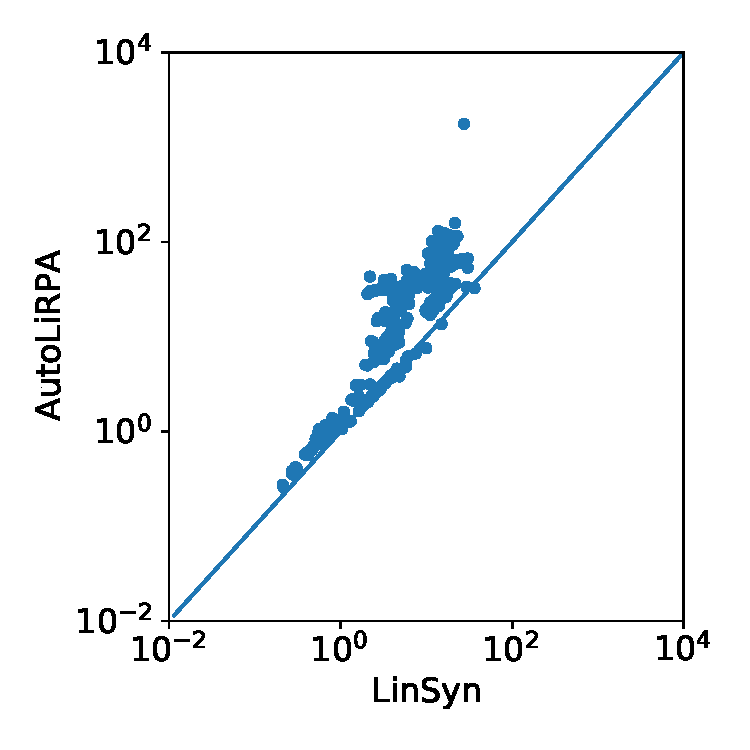
\includegraphics[width=\linewidth]{onlinesyn/figs/width_scatter.pdf}
		%
		\caption{Scatter plot comparing the final output interval width of
		\Name{} and~\autolipra{}.}
		\label{onlinesyn:fig:scatter-plot}
	\end{minipage}\hspace{24pt}%
	\begin{minipage}{.5\textwidth}
		\centering
%                \vspace{2ex}
		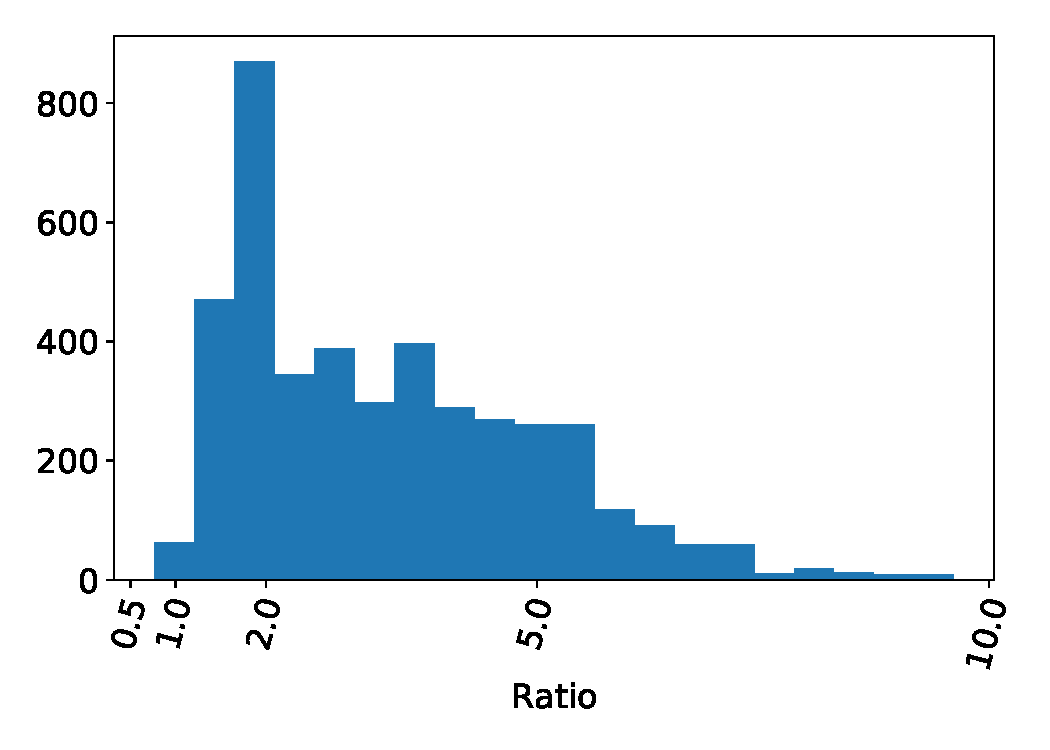
\includegraphics[width=\linewidth]{onlinesyn/figs/ratio_hist.pdf}
%                \vspace{1ex}

		\caption{Histogram of width ratios between \autolipra{} and \Name{}. Ratio reported as $
		\frac{\autolipra{}}{\Name{}} $.}
		\label{onlinesyn:fig:ratio-hist}
	\end{minipage}
\end{figure}

%\begin{figure}[t]
%	\centering
%	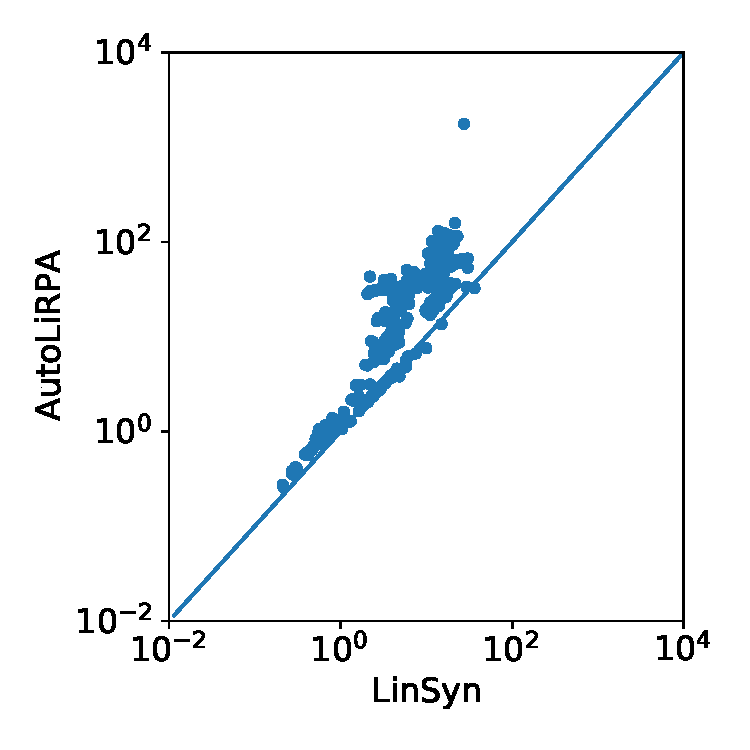
\includegraphics[width=0.5\linewidth]{onlinesyn/figs/width_scatter.pdf}
%	%
%	\caption{Comparing the accuracy of final outputs of \Name{}
%	and~\autolipra{}: each point above the diagonal line is a
%		winning case for our method.}
%	\label{onlinesyn:fig:scatter-plot}
%\end{figure}

Next, we perform a more in depth comparison of accuracy by comparing the widths
of the final output neuron's intervals that are computed by~\autolipra{}
and~\Name{}. The results are shown in the scatter plot in
Fig.~\ref{onlinesyn:fig:scatter-plot} and the histogram in
Fig.~\ref{onlinesyn:fig:ratio-hist}.
Each point in the scatter plot represents a single output neuron $ x_i
$ for a single verification problem. The $ x $-axis is the width of the
interval of the output neuron $ x_i $ (i.e. $ u_i - l_i $) computed by~\Name{},
and the $ y $-axis is the width computed by~\autolipra{}. A point above the
diagonal line
indicates that~\Name{} computed a tighter (smaller) final output interval.
%
In the histogram, we further illustrate the accuracy gain as the width ratio,
measured as $ \frac{\autolipra{}}{\Name{}} $.
%Note
%that, since the
%figure is in logarithmic scale, a slight diviation from the diagonal
%line means a significant win for our method.
%
Overall, the results show that~\Name{} is more accurate in nearly all cases,
and~\Name{} often produces final output bounds 2-5X tighter than~\autolipra{}.

%
%\section{Related Work}
%\label{onlinesyn:sec:related}

%\textit{Linear Bound-based Neural Network Verification}
%There is a large body of work on using linear-bounding
%techniques~\cite{SinghGPV19,zhang2018efficient,shi2020robustness,boopathy2019cnn,WengZCSHDBD18,paulsen2020reludiff,paulsen2020neurodiff,wu2021tightening,mohammadinejad2020diffrnn}
%and other abstract domains such as concrete intervals, symbolic
%intervals~\cite{WangPWYJ18}, and Zonotopes~\cite{GehrMDTCV18},
%for the purpose of neural network verification.
%%
%All of these can be thought of as leveraging restricted versions of the
%polyhedral abstract domain~\cite{CousotH78,CousotC77}.
%%
%%Such approaches can be thought
%%of as leveraging a restricted version of the polyhedral abstract
%%domain~\cite{CousotH78,CousotC77}. In addition, other abstract domains have
%%been leveraged as well, such as concrete intervals, symbolic
%%intervals~\cite{WangPWYJ18}, and Zonotopes~\cite{GehrMDTCV18}. All of these can
%%be thought
%%of as restricted versions of the full polyhedral domain.
%To the best
%of our knowledge, these approaches are the most scalable (in terms of network
%size) due to the use of approximations, but this also means they are less
%accurate than exact approaches. In addition, all these approaches have the
%limitation that they depend on bounds that are hand-crafted by an expert.
%%
%%For
%%example, DeepPoly~\cite{SinghGPV19}, a state-of-the-art tool based on linear
%%bounding, only handles the ReLU, sigmoid, tanh, and leaky ReLU activations.
%
%%There are also neural network verifiers based on over-approximated
%%interval analysis...  They rely on linear bounds to \emph{approximate}
%%the nonlinear activation functions...  Due to the use of
%%approximation, these techniques are often significantly faster than
%%SMT-solver based techniques; at the same time, they are also less
%%accurate.
%%%
%%The main problem is that, unlike our method, all of these existing
%%methods rely on linear bounds hand-crafted by domain experts.  As
%%such, they can only handle a very limited number of activation
%%functions used in the real world. For example, DeepPoly, which is a
%%state-of-the-art verification tool based on interval analysis, can
%%only handle \#\# types of activation functions.
%
%\textit{SMT solver-based Neural Network Verification}
%There is also a large body of work on using exact constraint solving for neural
%network verification. Early works include solvers specifically designed for
%neural networks, such as Reluplex and
%Marabou~\cite{KatzBDJK17,KatzHIJLLSTWZDK19} and others~\cite{DvijothamSGMK18},
%and leveraging existing
%solvers~\cite{Ehlers17,HuangKWW17,BastaniILVNC16,HuangKWW17,baluta2019quantitative,tjeng2019evaluating,hu2020reach}.
% While more accurate, the reliance on an SMT solver typically limits their
% scalability. More recent work
%often uses solvers to refine the bounds computed by linear
%bounding~\cite{Singh2019krelu,SinghGPV19iclr,WangPWYJ18nips,tran2019star,tran2020verification}.
%Since the solvers leveraged in these approaches usually involve linear
%constraint solving techniques, they are usually only applicable to piece-wise
%linear activation functions such as ReLU and Max/Min-pooling.
%To handle
%non-piece-wise linear activations, an expert would likely need to hand-craft
%the constraints.

%This is a large body of work on neural network verification based on the use
%of
%SMT solvers. Examples include ... and ...
%Unfortunately, due to the higher computational complexity, tools based on
%these
%techniques are often significantly slower, and the size of the networks that
%can be verified is signficantly smaller.

%\paragraph{Handling Arbitrary Activation Functions}
%
%To the best of our knowledge,~\autolipra{}~\cite{autolipra} is the only tool
%that attempts to automate the computation of linear
%bounds for arbitrary activation functions.  However, as mentioned
%earlier, its main disadvantage is that it must decompose complex activation
%functions into operations that it supports, which typically results in loose
%bounds. Our method, in contrast, overcomes this limitation and as a result, is
%significantly more accurate.

%\paragraph{Other Papers? or Future Work}
%
%Are there other papers that are closed related to our method?
%%
%If not, perhaps we can say a few words about future work
%on \emph{statically synthesizing the linear bounds}, as opposed to
%invoking the expensive solvers at run time for each given input
%region.



\section{Summary}
\label{onlinesyn:sec:conclusion}

We have presented~\Name{}, a method for synthesizing linear bounds for
arbitrary activation functions.
%
%Internally,~\Name{} relies on sampling and an
%LP solver to synthesize candidate linear bounds, and then
%leverages the SMT solver~\dReal{} to verify the soundness of the bounds,
%adjusting them if necessary.
%
The key advantage of~\Name{} is that it can handle complex
activation functions, such as Swish, GELU, and Log Log as a whole, allowing it
to synthesize much tighter linear bounds than existing tools.
%
Our experimental
results show this increased tightness leads to drastically increased certified
robustness, and tighter final output bounds.





\chapter{Offline Synthesis of Linear Approximations}
\label{ch:offlinesyn}
\declarecommand\bpnote[1]{\textcolor{blue}{{\textbf{Brandon Says: #1}}}}
\declarecommand\jwnote[1]{\textcolor{purple}{{\textbf{Jingbo Says: #1}}}}
\declarecommand\cwnote[1]{\textcolor{red}{{\textbf{Chao Says: #1}}}}

\declarecommand{\Name}{\textsc{LinSyn}}
\declarecommand{\ReluDiff}{\textsc{ReluDiff}}
\declarecommand{\ReluVal}{\textsc{ReluVal}}
\declarecommand{\DeepPoly}{\textsc{DeepPoly}}
\declarecommand{\Reluplex}{\textsc{Reluplex}}
\declarecommand{\Neurify}{\textsc{Neurify}}
\declarecommand{\Crown}{\textsc{Crown}}
\declarecommand{\Popqorn}{\textsc{Popqorn}}
\declarecommand{\RefineZono}{\textsc{RefineZono}}
\declarecommand{\dReal}{\textsc{dReal}}
\declarecommand{\autolipra}{\textsc{AutoLiRPA}}
\declarecommand{\popqorn}{\textsc{POPQORN}}

% NN verification is important due to adversarial behaviors
Neural networks have become a popular model choice in machine learning due to
their performance across a wide variety of tasks ranging from image
classification~\cite{he2016deep}, natural language
processing~\cite{vaswani2017attention}, and
control~\cite{hu2020reach,JulianKO18}. However, they are also
known to misclassify inputs in the presence of both small amounts of input
noise and seemingly insignificant perturbations to the
inputs~\cite{szegedy2013intriguing}. Indeed, many works have shown they are
vulnerable to a variety of seemingly benign input
transformations~\cite{engstrom2019exploring,kanbak2018geometric,alzantot2018generating},
which raises concerns about their deployment in safety-critical systems.
% Linear approximations have a wide range of applications,
% including NN verification
As a result, a large number of works have proposed verification techniques to
prove that a neural network is not vulnerable to these
perturbations~\cite{SinghGPV19,WangPWYJ18,WengZCSHDBD18}, or in
general satisfies some
specification~\cite{KatzBDJK17,KatzHIJLLSTWZDK19,hu2020reach}. Crucial to the
precision and scalability of these verification techniques are \textit{linear
approximations} of the network's activation functions.


% What is actually the problem?

In essence, given some arbitrary activation function $ \sigma(x) $, a linear
approximation is a \textit{coefficient generator function}
$ \mathcal{G}: (l, u) \to \langle a_l, b_l, a_u, b_u \rangle $, where $ l, u
\in \mathbb{R} $ are real values that correspond to the interval $ [l, u] $,
and $ a_l, b_l, a_u, b_u \in \mathbb{R} $ are real-valued coefficients
in the linear lower and upper bounds such that the following condition holds:
\begin{equation}
\begin{gathered}
\forall x \in [l, u]. \;\; a_l \cdot x + b_l \leq \sigma(x) \leq a_u
\cdot x + b_u
\end{gathered}
\end{equation}
Indeed, a key contribution in many seminal works on neural network verification
was a hand-crafted $ \mathcal{G}(l, u)
$~\cite{SinghGPV19,WangPWYJ18,WangPWYJ18nips,balunovic2019certifying,du2021cert,ko2019popqorn,zhang2018efficient,WengZCSHDBD18,wu2021tightening,ryou2021scalable,shi2020robustness}
and follow-up work built off these
hand-crafted
approximations~\cite{KatzHIJLLSTWZDK19,tjeng2019evaluating,SinghGPV19iclr,Singh2019krelu}.
Furthermore, linear approximations have applications beyond neural network
verification, such as rigorous global optimization and
verification~\cite{lebbah2007efficient,trombettoni2011inner}.

However, crafting $ \mathcal{G}(l, u) $ is tedious, error-prone, and requires
an expert. Unfortunately, in the case of neural network activation functions,
experts have only crafted approximations for the most common functions, namely
ReLU, sigmoid, tanh, max-pooling, and those in vanilla LSTMs. As a result,
existing techniques cannot handle new and cutting-edge activation functions,
such as Swish~\cite{ramachandran2017searching},
GELU~\cite{hendrycks2016gaussian}, Mish~\cite{misra2019mish}, and
LiSHT~\cite{roy2019lisht}.

In this work, we consider the problem of automatically synthesizing the coefficient generator function
$\mathcal{G}(l, u) $, which can alternatively be viewed as four individual
functions $\mathcal{G}_{a_l}(l,u)$, $\mathcal{G}_{b_l}(l,u)$,
$\mathcal{G}_{a_u}(l,u)$, and $\mathcal{G}_{b_u}(l,u)$, one
for each
coefficient.
However, synthesizing the generator functions is a challenging task because (1)
the search space for each function is very large (in fact, technically
infinite), (2) the optimal generator functions are highly nonlinear for all
activation functions considered both in our work and prior work, and (3) to
prove soundness of the synthesized generator functions, we must show:
\begin{equation}
\begin{gathered}\label{offlinesyn:eq:intro-sound}
\forall [l, u] \in \mathbb{IR}, x \in [l, u] ~.\\
(\mathcal{G}_{a_l}(l,u) \cdot x + \mathcal{G}_{b_l}(l,u))
\leq \sigma(x) \leq
(\mathcal{G}_{a_u}(l,u) \cdot x + \mathcal{G}_{b_u}(l,u))
\end{gathered}
\end{equation}
where $ \mathbb{IR} = \{[l, u] ~|~ l, u \in \mathbb{R}, l \leq u \} $ is the
set of all real intervals. The above equation has
highly non-linear constraints, which cannot be directly handled by
standard verification tools, such as the Z3~\cite{de2008z3} SMT solver.

%\textcolor{red}{Synthesizing such generator functions is  a challenging task
%for two reasons.
%%
%First, it is difficult to find generator functions that can produce
%tight linear bounds for a wide range of input intervals.
%%
%Second, it is difficult to prove that the generator functions are
%sound.  While the resulting bounds are linear in terms of $x$, the
%generator functions themselves may be highly non-linear in terms of
%$l$ and $u$.  To ensure that the linear bounds are sound for all
%possible ways of instantiating $l$ and $u$, we must prove the
%soundness of the generator functions as follows:
%%
%\begin{equation}
%\begin{gathered}\label{offlinesyn:eq:intro-sound}
%\forall x \in [l, u]  ~.~
%  (\mathcal{G}_{c^l_1}(l,u) \cdot x + \mathcal{G}_{c^l_2}(l,u))
%  \leq \sigma(x) \leq
%  (\mathcal{G}_{c^u_1}(l,u) \cdot x + \mathcal{G}_{c^u_2}(l,u))
%\end{gathered}
%\end{equation}
%%
%However, such non-linear constraints cannot be directly handled by
%standard verification tools, such as the Z3 SMT solver.
%%
%}


To solve the problem, we propose a novel example-guided synthesis and
verification approach, which is applicable to any differentiable,
Lipschitz-continuous activation function $ \sigma(x) $. (We note that
activation functions are typically required to be differentiable and
Lipschitz-continuous in order to be trained by gradient descent, thus our
approach applies to any \textit{practical} activation function).
%
To tackle the potentially infinite search space of $ \mathcal{G}(l, u) $, we
first propose two \textit{templates} for $ \mathcal{G}(l, u) $, which are
inspired by the hand-crafted coefficient functions of prior work.
%
The ``holes'' in each template are filled by a machine learning model, in our
case a small neural network or linear regression model.
%
Then, the first step is to partition the input space of $ \mathcal{G}(l,
u) $, and then assign a single template to each subset in the partition.
%
The second step is to fill in the holes of each template. Our approach
leverages an example-generation procedure to produce a large number of training
examples of the form $((l, u), (a_l, b_l, a_u, b_u)) $, which can then be used
to train the machine learning component in the template.
%
However, a template instantiated with a trained model may still violate
Equation~\ref{offlinesyn:eq:intro-sound}, specifically the lower bound (resp.
upper bound) may be above (resp. below) the activation function over some
interval $ [l, u] $.
%
To ensure soundness, the final step is to bound the
\textit{maximum violation} of a particular template instance using a rigorous
global optimization technique based on interval analysis, which is implemented
by the tool IbexOpt~\cite{chabert2009contractor}.
%
We then use the computed maximum violation to adjust the template to ensure
Equation~\ref{offlinesyn:eq:intro-sound} always holds.

\begin{figure}[t]
\centering
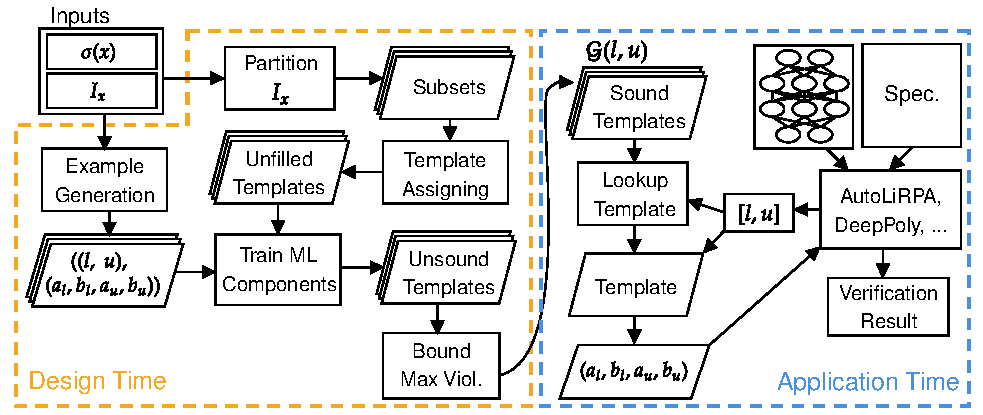
\includegraphics[width=.95\linewidth]{offlinesyn/figs/flow.pdf}
\caption{Overview of our method for synthesizing the \emph{coefficient generator
function}.}
\label{offlinesyn:fig:overview}
\end{figure}

The overall flow of our method is shown in Figure~\ref{offlinesyn:fig:overview}.
%
It takes as input the activation function $ \sigma(x) $, and the set of input
intervals $ I_x \subseteq \mathbb{IR} $ for which $ \mathcal{G}(l, u) $ will be
valid.
%
During \textit{design time}, we follow the previously described approach, which
outputs a set of sound, instantiated templates which make up $ \mathcal{G}(l,
u) $. Then the synthesized $ \mathcal{G}(l, u) $ is integrated into an existing
verification tool such as~\autolipra{}~\cite{autolipra}
or~\DeepPoly{}~\cite{SinghGPV19}.
These tools take as input a neural network and a specification, and output the
verification result (proved, counterexample, or unknown).
%
At \textit{application time} (i.e., when attempting to verify the input
specification), when these tools need a linear approximation for
$ \sigma(x) $ over the interval $ [l, u] $, we lookup the appropriate template
instance, and use it to compute the linear approximation $(a_l, b_l, a_u, b_u)$,
and return it to the tool.

To the best of our knowledge, our method is the first to synthesize a linear
approximation generator function $ \mathcal{G}(l, u) $ for any given activation function $ \sigma(x)
$. Our approach is fundamentally different from the ones used by state-of-the-art neural network verification tools such as~\autolipra{}
and~\DeepPoly{}, which require an expert to hand-craft the approximations. We
note that, while~\autolipra{} can handle activations that it does not
explicitly support by \textit{decomposing} $ \sigma(x) $ into
elementary operations for which it has (hand-crafted) linear approximations,
and then combining them, the resulting bounds are often not tight.
In contrast, our method synthesizes linear approximations for $
\sigma(x) $ as a whole, and we show experimentally that our synthesized
approximations significantly outperform~\autolipra{}.

%We note that our method is fundamentally different from existing approaches
%such as~\DeepPoly{}~\cite{SinghGPV19},~\autolipra{}~\cite{autolipra},
%and~\popqorn{}.
%Our method is fundamentally different from existing approaches adopted
%by tools
%%
%\textcolor{red}{
%%
%such as \DeepPoly{}, \popqorn{} and \autolipra{}.
%%
%Specifically, \DeepPoly{} ...
%%
%\popqorn{}...
%%
%\autolipra{}...
%%
%In contrast, our method synthesizes a \emph{bounds-generating
%function} capable of producing sound and tight linear bounds at run
%time for any concrete interval $[l,u]$.
%%
%}


We have implemented our approach and evaluated it on popular neural
network verification problems (specifically, robustness verification problems in the presence of input perturbations).
Compared against state-of-the-art linear approximation based
verification tools, our synthesized linear approximations can drastically
outperform these existing tools in terms of the number of problems verified on
recently published activation functions such as Swish~\cite{ramachandran2017searching},
GELU~\cite{hendrycks2016gaussian}, Mish~\cite{misra2019mish}, and
LiSHT~\cite{roy2019lisht}.

To summarize, we make the following contributions:
\begin{itemize}
	\item We propose the first method for synthesizing the linear
	approximation generator function $ \mathcal{G}(l, u) $ for any given activation function.
	\item We implement our method, use it to synthesize linear approximations
	for several novel activation functions, and integrate these approximations
	into a state-of-the-art neural network verification tool.
	\item We evaluate our method on a large number of neural network
	verification problems, and
	show that our synthesized approximations significantly outperform
	the state-of-the-art tools.
\end{itemize}



\section{Preliminaries}
\label{offlinesyn:sec:preliminaries}

In this section, we discuss background knowledge necessary to understand our
work. Throughout the paper, we will use the following notations: for variables or scalars we use lower
case letters (e.g., $ x \in \mathbb{R} $), for vectors we use bold lower case
letters (e.g., $ \mathbf{x} \in \mathbb{R}^n $) and for matrices we use bold
upper case letters (e.g., $ \mathbf{W} \in \mathbb{R}^{n \times m} $). In
addition, we use standard interval notation: we let $ [l,u] = \{x \in
\mathbb{R}| l \leq x \leq u \} $ be a real-valued interval, we denote the set
of all real intervals as $
\mathbb{IR} = \{[l,u] | l, u \in \mathbb{R}, l \leq u\} $, and finally we
define the set of $ n $-dimensional intervals as
$ \mathbb{IR}^n = \{
\bigtimes_{i=1}^n [l_i, u_i] \; | \; [l_i, u_i] \in \mathbb{IR} \} $, where $
\bigtimes $ is the Cartesian product.

\subsection{Neural Networks}

We consider a neural network to be a function $ f: \mathbb{X} \subseteq
\mathbb{R}^n \to \mathbb{Y} \subseteq \mathbb{R}^m $, which has $ n $ inputs
and $ m $ outputs.
%
\begin{comment}
$ \mathbb{X} $ may be, for example, the set of all images, and an
input $ \mathbf{x} \in \mathbb{X} $ would be the pixels of an image
flattened into a vector. We focus on neural networks classifiers where
each element in the output vector $ f(\mathbf{x})
\in \mathbb{Y} $ represents a score for one of $ m $ classes, and the highest
score is the predicted class.
\end{comment}
%
For ease of presentation, we focus the discussion
on \textit{feed-forward, fully-connected} neural networks (although
the bounds synthesized by our method apply to all neural
network architectures).
%
For $ \mathbf{x} \in \mathbb{X} $, such networks compute $ f(\mathbf{x}) $ by
performing an alternating
series of matrix multiplications followed by the element-wise
application of an activation function $
\sigma(x) $.


Formally, an $ l $-layer neural network with $ k_i $ neurons in each
layer (and letting $ k_0 = n, k_l = m $) has $ l $ weight matrices
and bias vectors $ \mathbf{W}_i \in \mathbb{R}^{k_{i-1} \times k_i} $
and $ \mathbf{b}_i
\in \mathbb{R}^{k_{i}} $ for $ i \in \{1..l\} $. The input of the network is $
f_0 =
\mathbf{x}^T $, and the output of layer $ i $ is given by the function:
$ f_i = \sigma(f_{i-1} \cdot \mathbf{W}_i + \mathbf{b}_i) $
which can be applied recursively until the output layer of the network is reached.

Initially, common choices for the activation function $ \sigma(x) $ were $ ReLU(x) = max(0, x) $, $
sigmoid(x) = \frac{e^x}{e^x + 1} $, and $ tanh(x) = \frac{e^x - e^{-x}}{e^x +
e^{-x}}  $, however the field has advanced rapidly in recent years and, as a result,
automatically discovering novel activations has become a
research subfield of its own~\cite{ramachandran2017searching}. Many recently proposed activations,
such as Swish and GELU~\cite{ramachandran2017searching,hendrycks2016gaussian},
have been shown to outperform the common choices in important machine learning tasks.


\subsection{Existing Neural Network Verification Techniques and Limitations}

We consider neural network verification problems of the following form: given a neural
network $ f : \mathbb{X} \to \mathbb{Y} $ and an input set $ X \subseteq
\mathbb{X} $, compute an over-approximation $ Y $ such that $ \{f(\mathbf{x}) \mid
\mathbf{x} \in X \} \subseteq Y \subseteq \mathbb{Y} $.
%
The most scalable approaches to neural network verification
(where scale is measured by number of neurons in the network)
 use linear bounding techniques to compute
$ Y $, which require a \textit{linear approximation} of the network's
activation function.
%
This is an extension of \textit{interval
analysis}~\cite{moore2009introduction} (e.g., intervals with linear
lower/upper bounds~\cite{SinghGPV19,autolipra}) to compute $ Y $, and thus
$ X $ and $ Y $ are represented as elements of $
\mathbb{IR}^n $ and $ \mathbb{IR}^m $, respectively.

\begin{comment}
In classification, we are typically interested in showing that for
some set of inputs $ X \subseteq
\mathbb{R} $, $ f $ always produces the same classification. If $ j \in
\{1..m\} $ is the target class, and we
compute $ Y = \bigtimes_{i=1}^m [l_i, u_i] $, then this amounts to checking
that $ l_j > u_i, i \neq j, i \in \{1..m\} $ (i.e., class $ j $'s lower bound is
greater than all other classes upper bound).
\end{comment}

We use Figure~\ref{offlinesyn:fig:motex} to illustrate a typical neural network
verification problem.
The network has input neurons $ x_1, x_2 $,
output neurons $ x_7, x_8 $ and a single hidden layer. We assume the activation
function is $ swish(x) = x \cdot sigmoid(x) $, which is shown by the blue line
in Figure~\ref{offlinesyn:fig:motex-linapprox}. Our input space is $ X = [-1, 1]
\times
[-1, 1] $ (i.e., $ x_1, x_2 \in [-1, 1] $), and we want to prove  $
x_7 > x_8 $, which can be accomplished by first computing the bounds $ x_7 \in [l_7, u_7],
x_8 \in [l_8, u_8] $, and then showing $ l_7 > u_8 $. Following the prior
work~\cite{SinghGPV19} and for simplicity, we split the affine transformation
and application of activation function in the hidden layer into two steps, and we assume the
neurons $ x_i$, where $i \in \{1..8\} $, are ordered such that $ i < j $ implies that $
x_i $ is in either the same layer as $ x_j $, or a layer prior to $ x_j $.

\begin{figure}[t]
\centering
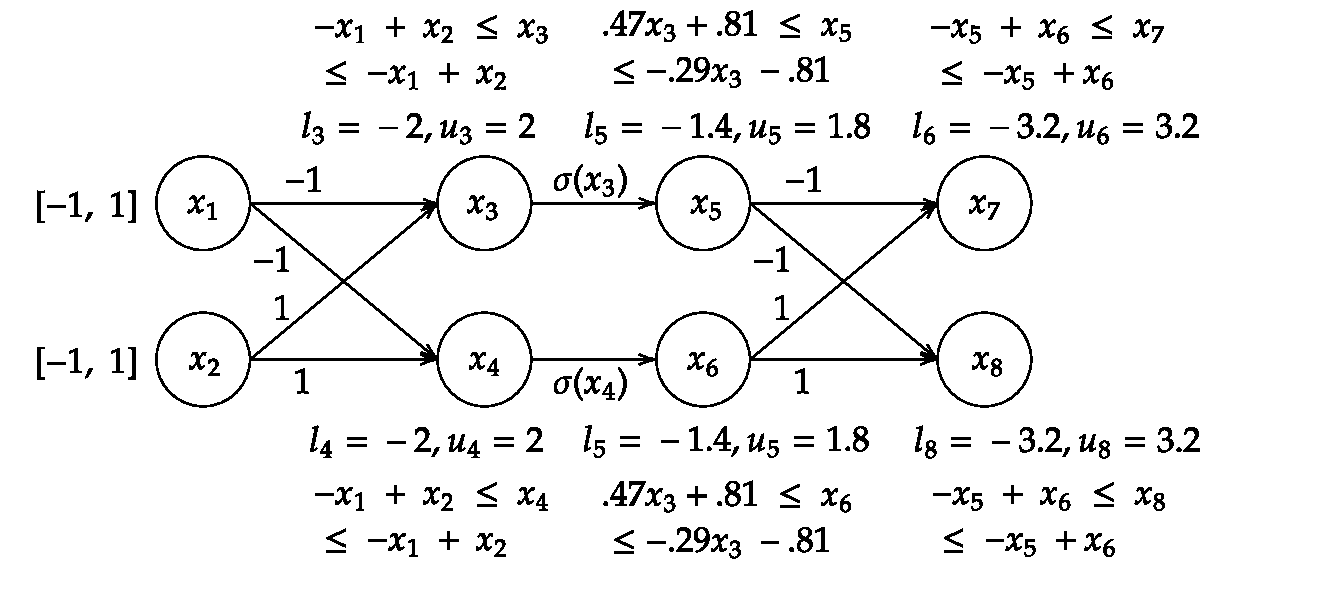
\includegraphics[width=0.9\linewidth]{offlinesyn/figs/motex.pdf}
\caption{An example of linear bounding for neural network verification.
\label{offlinesyn:fig:motex}}
\end{figure}

Linear bounding based neural network verification techniques work as follows.
For each neuron $
x_i $, they compute the concrete lower and upper bounds $ l_i$ and $u_i $,
together with symbolic
lower and upper bounds.  The symbolic lower and upper bounds are linear constraints $
\sum_{j=0}^{i-1} c^l_j \cdot x_j + c^l_i \leq x_i \leq \sum_{j=0}^{i-1} c^u_j
\cdot x_j + c^u_i $, where each of $ c^l_i, c^u_i $ is a constant. Both bounds are
computed in a forward layer-by-layer fashion, using the result of the previous
layers to compute bounds for the current layer.

We illustrate the computation in Figure~\ref{offlinesyn:fig:motex}. In the
beginning, we have $
x_1 \in [-1, 1] $ as the concrete bounds, and $ -1 \leq x_1 \leq 1 $ as the
symbolic  bounds, and similarly for $ x_2 $. To obtain bounds for $ x_3, x_4 $, we
multiply $ x_1, x_2 $ by the edge weights, which for $ x_3 $ gives the linear
bounds $ -x_1 + x_2 \leq x_3 \leq -x_1 + x_2 $ . Then, to compute $ l_3 $ and $
u_3 $, we minimize and maximize the linear lower and upper bounds,
respectively, over $ x_1, x_2 \in [-1, 1] $. Doing so results in $ l_3 = -2,
u_3 = 2 $. We obtain the same result for $ x_4 $.

However, we encounter a key challenge when attempting to bound $ x_5 $, as
we need a linear approximation of $ \sigma(x_3) $ over $ [l_3, u_3] $ when
bounding $ x_5 $, and similarly for $ x_6 $. Here, a linear approximation
for $ x_5 $ can be regarded as a set of coefficients $ a_l, b_l, a_u, b_u $ such that the
following \textit{soundness} condition holds: $ \forall x_3 \in
[l_3, u_3] ~.~ a_l \cdot x_3 + b_l \leq \sigma(x_3) \leq a_u \cdot
x_3 + b_u $.
%
In addition, a sub goal for the bounds is \textit{tightness},
which typically means the volume between the bounds and $ \sigma(x) $ is
minimized.
%
Crafting a function to generate these coefficients has been the
subject of many prior works. Many seminal papers on neural network verification
have focused on solving this problem alone. Broadly speaking, they fall into
the following categories.


\paragraph{Hand-crafted Approximation Techniques} The first category of
techniques use hand-crafted functions for generating $ a_l, b_l, a_u, b_u $.
Hand-crafted functions are generally fast because they are static, and tight
because an expert designed them.
%
Unfortunately, current works in this category are not \textit{general} -- they
only considered the most common activation functions, and thus cannot currently
handle our motivating example or any recent, novel activation functions.
%
For these works to apply to our motivating example, an expert would need to hand-craft an
approximation for the activation function, which is both difficult and error-prone.

\paragraph{Expensive Solver-Aided Techniques}
The second category use expensive solvers and optimization tools to compute
sound and tight bounds in a general way, but at the cost of runtime.
%
Recent works include DiffRNN~\cite{mohammadinejad2020diffrnn} and
POPQORN~\cite{ko2019popqorn}. The former uses (unsound) optimization to
synthesize candidate coefficients and then uses an SMT solver to
verify soundness of the bounds. The latter uses constrained-gradient descent to
compute coefficients. We note that, while these works do not
explicitly target an arbitrary activation function $ \sigma(x) $, their
techniques can be naturally extended.
%
Their high runtime and computational cost are undesirable and, in general, make
them less scalable than the first category.

%\begin{wrapfigure}{R}{0.5\textwidth}
\begin{figure}[t]
	\centering
%	\vspace{-2ex}
	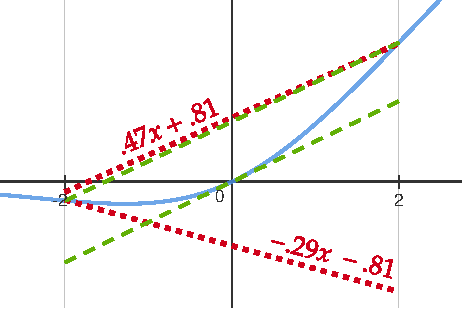
\includegraphics[width=.5\linewidth]{offlinesyn/figs/motex-linapprox.pdf}
	\caption{Approximation of~\autolipra{} (red) and our approach
		(green).\label{offlinesyn:fig:motex-linapprox}}
\end{figure}
%\end{wrapfigure}
\paragraph{Decomposing Based Techniques} The third category combine
hand-crafted approximations with a decomposing based technique to obtain
generality and efficiency, but at the cost of tightness. Interestingly, this is
similar to the approach used by nonlinear SMT solvers and optimizers such as
dReal~\cite{gao2013dreal} and Ibex~\cite{chabert2009contractor}.
%
To the best of our knowledge, only one
work~\autolipra{}~\cite{autolipra} implements this approach for neural network
verification.
%
Illustrating on our example,~\autolipra{} does not have a static linear
approximation for $ \sigma(x_3) = x_3 \cdot sigmoid(x_3) $, but it has
static approximations for $ sigmoid(x_3) $ and $ x_3 \cdot y $.
%
Thus we can
bound $ sigmoid(x_3) $ over $ x_3 \in [-2,2] $, and then, letting $ y =
sigmoid(x_3) $, bound $ x_3 \cdot y $. Doing so results in the approximation
shown as red lines in Figure~\ref{offlinesyn:fig:motex-linapprox}.
%
While useful, they are
suboptimal because they do not minimize the area between the two bounding
lines. This suboptimality occurs due to the decomposing, i.e., the static
approximations used here were not designed for $ swish(x) $ as a whole, but designed
for the individual elementary operations.

\paragraph{Our Work: Synthesizing Static Approximations} Our work overcomes the
limitation of prior work by automatically synthesizing a \textit{static}
function specifically for any given activation function $ \sigma(x) $
\textit{without} decomposing. Since the
synthesis is automatic, and results in a bound generator function, we obtain generality
and efficiency, and since the synthesis targets $ \sigma(x) $ specifically, we
\textit{usually} (demonstrated empirically) obtain tightness.
%
In Figure~\ref{offlinesyn:fig:motex-linapprox}, for example, the bounds computed
by our method are represented by the green lines.
%
The synthesized bound generator function can then be integrated
to state-of-the-art neural network verification tools, including \autolipra{}.

\paragraph{Wrapping Up the Example}
For our running example, using~\autolipra{}'s linear approximation,
we would add the linear bounds for $ x_5 $ shown in
Figure~\ref{offlinesyn:fig:motex}. To
compute $ l_5, u_5 $, we would substitute the linear bounds for $ x_3 $ into $
x_5 $'s linear bounds, resulting in linear bounds with only $ x_1, x_2 $ terms
that can be minimized/maximized for $ l_5, l_6 $ respectively. We do the same
for $ x_6 $, and then we repeat the entire process until the output layer is
reached.

\section{Problem Statement and Challenges}

In this section, we formally define the synthesis problem and then explain the
technical challenges.
%
During the discussion, we focus on synthesizing the generator
functions for the upper bound. We note that we can synthesize lower bound
generator functions analogously.
%

\subsection{The Synthesis Problem}
\label{offlinesyn:sec:synthesis-problem}

Given an activation function $ \sigma(x) $ and an input universe $ x
\in [l_x, u_x] $, we define the set of all intervals over $ x $ in this universe
as $ I_x = \{ \; [l, u] \;|\; [l, u] \in \mathbb{IR}, l, u \in [l_x, u_x] \}$.
(In our experiments, for instance, we use $ l_x = -10$ and $u_x = 10 $).


Our goal is to synthesize a generator function $\mathcal{G}:
(l,u)\to \langle a_u,b_u\rangle$, or equivalently, two generator
functions $\mathcal{G}_{a_u}(l,u)$ and $\mathcal{G}_{b_u}(l,u)$ such that
%
$\forall [l, u] \in I_x, x \in \mathbb{R}$, the condition $
  x \in [l, u] \implies  \sigma(x) \leq \mathcal{G}_{a_u}(l, u) \cdot x
  +\mathcal{G}_{b_u}(l,u)
$ holds.
%
This is the same as requiring that the following condition does
\textbf{not} hold (i.e., the formula is unsatisfiable):
%
\begin{gather*}\label{offlinesyn:eq:sound}
\exists [l, u] \in I_x, x \in \mathbb{R} ~.~ x \in [l, u] \wedge \sigma(x) >
\mathcal{G}_{a_u}(l, u) \cdot x +
\mathcal{G}_{b_u}(l,u)
\end{gather*}
The formula above expresses the search for a counterexample, i.e., an input interval $
[l, u] $ such that $ \mathcal{G}_{a_u}(l, u) \cdot x + \mathcal{G}_{b_u}(l, u)
$ is not a sound upper bound of $\sigma(x) $ over the interval $ [l, u] $.
%
Thus, if the above formula is unsatisfiable, the soundness of the coefficient
functions $ \mathcal{G}_{a_u}, \mathcal{G}_{b_u} $ is proved.
%The first  conjunct ($ l < u $)
%restricts the search space to only valid input intervals. The next two
%conjuncts ($ l \leq x \wedge x \leq u \; $) ensure the validity of the
%counterexample. The last conjunct expresses the unsoundness of the upper bound
%for a given input interval $ [l, u] $ at point $ x $.
%
%Alternatively, we can
%view our goal as finding $ a_u, b_u $ such that the following \textbf{does}
%hold:
%\begin{gather*}
%\forall l \in [l_x, u_x], u \in [l_x, u_x], x \in [l_x, u_x] \\
%l \geq u \vee l > x \vee x > u \; \vee \\
%\sigma(x) \leq a_u(l, u)x + b_u(l, u)
%\end{gather*}

In addition to \textit{soundness}, we want the bound to be \textit{tight},
which in our context has two complementary goals.
%
For a given $ [l, u] \in I_x $ we should have (1) $
\sigma(z) = \mathcal{G}_{a_u}(l, u) \cdot z + \mathcal{G}_{b_u}(l, u) $ for at
least one $ z \in [l, u] $ (i.e., the bound touches $ \sigma(x) $ at
some point $ z $),
%
and (2) the volume below $ \mathcal{G}_{a_u}(l, u) \cdot x +
\mathcal{G}_{b_u}(l, u) $ should be minimized (which we note is equivalent to
minimizing the volume between the upper bound and $\sigma(x)$ since $\sigma(x)$ is fixed).
%
We will illustrate the volume by the shaded green region below the dashed
bounding line in Figure~\ref{offlinesyn:fig:samplelp}.


The first goal is intuitive: if the bound does not touch $
\sigma(x) $, then it can be shifted downward by some constant. The second goal
is a heuristic taken from prior work that has been shown to yield a precise
approximation of the neural network's output set.
%TODO: introduce tightness (in preliminaries?)


\subsection{Challenges and Our Solution}

We face three challenges in searching for the generator functions $
\mathcal{G}_{a_u}$ and $ \mathcal{G}_{b_u} $. First, we must restrict
the search space so that a candidate can be found in a reasonable amount of
time (i.e., the search is tractable). The second challenge, which is at odds
with the first, is that we must have a large enough search space such that it
permits candidates that represent tight bounds.
%If our search space is
%overly-restricted the synthesized $ \mathcal{G}_{a_u}, \mathcal{G}_{b_u} $ may
%be useless.
Finally, the
third challenge, which is at odds with the second, is that we must be able to
formally verify $ \mathcal{G}_{a_u}, \mathcal{G}_{b_u} $ to be sound. While
more complex geneator functions ($ \mathcal{G}_{a_u}, \mathcal{G}_{b_u} $) will
likely
produce tighter bounds, they will be more difficult (if not
impractical) to verify.

%\begin{wrapfigure}{R}{0.5\textwidth}
\begin{figure}[t]
	\centering
%	\vspace{-2ex}
	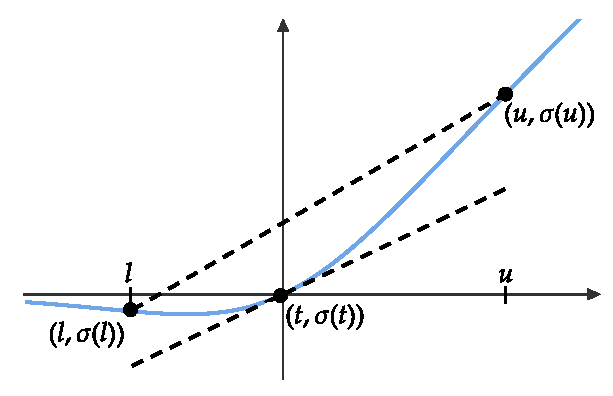
\includegraphics[width=0.5\linewidth]{offlinesyn/figs/twopt_tanpt.pdf}
	\caption{Illustration of the two-point form bound (upper dashed line) and
	tangent-line form bound (lower dashed line).\label{offlinesyn:fig:twopttanpt}}
%	\vspace{-2ex}
\end{figure}
%\end{wrapfigure}
We tackle these challenges by proposing two templates for $ \mathcal{G}_{a_u},
\mathcal{G}_{b_u} $ and then
developing an approach for selecting the appropriate template.
%
We observe that prior work has always expressed the linear bound for $
\sigma(x) $ over an interval $ x \in [l, u] $
%We observe that
%linear bounds of a 1-D activation function $ \sigma(x) $ over a region $ x \in
%[l, u] $ can usually be expressed
as either the line connecting the points $ (l, \sigma(l)), (u, \sigma(u)) $,
referred to as the \textit{two-point form}, or as the line tangent to $
\sigma(x) $ at a point $ t $, referred to as \textit{tangent-line form}.
%
We illustrate both forms in
Figure~\ref{offlinesyn:fig:twopttanpt}.
Assuming that $ \sigma'(x) $ is the derivative of $ \sigma(x) $,
the two templates for $ \mathcal{G}_{a_u}$ and $\mathcal{G}_{b_u} $ as follows:
\begin{align}
\begin{aligned}
&\mathcal{G}_{a_u}(l, u) = \frac{\sigma(u) - \sigma(l)}{u - l} \\
&\mathcal{G}_{b_u}(l, u) = - \mathcal{G}_{a_u}(l, u) \cdot l + \sigma(l) +
\epsilon
\end{aligned} &\hspace{36pt}
\begin{aligned}
\text{two-point}\\
\text{form template}
\end{aligned}
\label{offlinesyn:eq:template-2pt}\\[2ex]
\begin{aligned}
&\mathcal{G}_{a_u}(l, u) = \sigma'(g(l, u)) \\
&\mathcal{G}_{b_u}(l, u) = -\mathcal{G}_{a_u}(l, u) \cdot g(l, u) +
\sigma(g(l, u)) + \epsilon
\end{aligned} &\hspace{36pt}
\begin{aligned}
\text{tangent-line}\\
\text{form template}
\end{aligned}
\label{offlinesyn:eq:template-tan}
\end{align}
In these templates, there are two \emph{holes} to fill during synthesis:
$ \epsilon $ and $ g(l, u) $. Here, $\epsilon $
is a real-valued constant upward (positive) shift that ensures soundness of the
linear bounds computed by both templates.
%
We compute $ \epsilon $ when we verify the soundness of the template (discussed
in Section~\ref{offlinesyn:sec:soundness}).
%
In addition to $\epsilon$, for the
tangent-line template, we must synthesize a function $ g(l, u) = t$, which
takes the interval $ [l, u] $ as input and returns the tangent point $ t $ as output.
%
%Since the function $g(l,u)$ is different for each activation function
%$\sigma(x)$, it must be synthesized by our method.

These two templates, together, address the previously mentioned three challenges. For the
first challenge, the two-point form actually does not have a search space, and thus can be computed efficiently, and
for the tangent-line form, we only need to synthesize the function $g(l,u)$. In
Section~\ref{offlinesyn:sec:learning}, we will show empirically that $ g(l, u) $
tends to be
much easier to learn than a function that directly predicts the coefficients $
a_u, b_u $.
%
For the second
challenge, if the two-point form is sound, then it is also tight since the
bound touches $ \sigma(x) $ by construction. Similarly, the tangent-line form
touches $ \sigma(x) $ at $ t $.
%
For the third challenge, we will show empirically that these templates can be
verified to be sound in a reasonable amount of time (on the order of an hour).
%Finally, for the third challenge, by
%formulating the templates in this way, we can exploit the convex/concave
%regions of $ \sigma(x) $ to
%%implicitly verify
%prove the soundness of $ \mathcal{G}_{a_u}, \mathcal{G}_{b_u} $ for large
%regions of their input
%space without calling a verifier.

%However, taking this approach requires us to decide which one to use for a
%given input interval $ [l, u] $.
%
At a high level, our approach contains three steps.
The first step is to partition $ I_x $ into subsets, and then for each
subset we assign a fixed template -- either the two-point form template or
tangent-line form template.
%
The advantage of partitioning is two-fold. First, no single template is a
good fit for the entire $ I_x $, and thus partitioning results in overall
tighter bounds.
%
And second, if the final verified template for a particular
subset has a large violation (which results in a large upward shift and thus
less tight bounds) the effect is localized to that subset only.
%We collectively
%refer to the union of all subsets assigned a two-point form template as $
%I_{2pt} $, and the union of all subsets assigned a tangent-point form template
%as $ I_{tan} $. Note that $ I_{2pt} \cup I_{tan} = I_x $ and $ I_{2pt} \cap
%I_{tan} = \emptyset$.
Once we have assigned a template to each subset of $ I_x $, the second step is
to learn a $ g(l, u) $ for each subset that was assigned a tangent-line
template. We use an example-generation procedure to generate training examples,
which are then used to train a machine learning model.
%
After learning each $ g(l, u) $, the third step is to compute $ \epsilon $ for
all of the templates. We phrase the search for a sound $ \epsilon $ as a
nonlinear global optimization problem, and then use the interval-based solver
IbexOpt~\cite{chabert2009contractor} to bound $ \epsilon $.

%Letting $ \sigma'(x) $ be the first derivative of $ \sigma(x) $, we define
%our templates for $ a_u, b_u $ as follows:
%\begin{align}
%	\begin{aligned}
%		&a_u(l, u) = \frac{\sigma(u) - \sigma(l)}{u - l} \\
% 		&b_u(l, u) = - a_u(l, u) \times l + \sigma(l) + \epsilon
%	\end{aligned} &\hspace{36pt}
%	\text{two-point template}
%%	\; \text{if} \; (l, u) \in I_{2pt}
%	\label{offlinesyn:eq:template-2pt}\\[2ex]
%	\begin{aligned}
%		&a_u(l, u) = \sigma'(g(l, u)) \\
%		&b_u(l, u) = -a_u(l, u) \times g(l, u) + \sigma(g(l, u)) + \epsilon
%	\end{aligned} &\hspace{36pt}
%	\text{tangent-point template}
%%	\; \text{if} \; (l, u) \in I_{tan}
%	\label{offlinesyn:eq:template-tan}
%\end{align}
%%
%Here, $\epsilon$ is a small shift (constant value) computed by our
%method at the design time in order to make the overall bound sound.
%%
%Once we have this partition, the next step is to synthesize the
%function $ g(l, u) $ over $ I_{tan} $ that results in tight
%bounds. Then, we verify that the bounds are sound and, if necessary, adjust the
%coefficient functions to ensure soundness.



\section{Our Approach}
\label{offlinesyn:sec:method-1}

In this section, we first present our method for partitioning $ I_x $,
the input interval space, into disjoint subsets and then assigning a
template to each subset. Then, we present the method for synthesizing
the bounds-generating function for a subset in the partition of
$I_x$ (see Section~\ref{offlinesyn:sec:synthesis-problem}).
Next, we present the method for making the bounds-generating
functions sound. Finally, we present the method for efficiently
looking up the appropriate template at runtime.

%\begin{wrapfigure}{R}{0.5\textwidth}
\begin{figure}[t]
	\centering
%	\vspace{-2ex}
	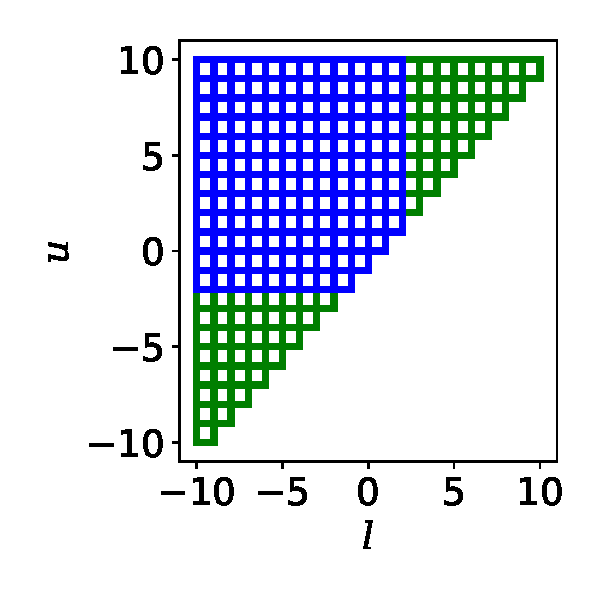
\includegraphics[width=0.4\linewidth]{offlinesyn/figs/partition.pdf}
	\caption{Partition of $ I_x $ for the Swish activation function, where the blue boxes belong
	to $ I_{tan} $, and the green boxes belong to $ I_{2pt} $.
	\label{offlinesyn:fig:partition}}
%	\vspace{-3ex}
\end{figure}
%\end{wrapfigure}

\subsection{Partitioning the Input Interval Space ($I_x$)}

A key consideration when partitioning $ I_x $ is how to represent each disjoint
subset of input intervals. While we could use a highly expressive representation such as polytope
or even use non-linear constraints, for efficiency reasons, we represent each
subset (of input intervals) as a box. Since a subset uses either the two-point
form template or the tangent-line form template, the input interval space can
be divided into
$I_x = I_{2pt}\cup I_{tan}$.
%
Each of $I_{2pt} $ and $ I_{tan} $ is  a set of boxes.


At a high-level, our
approach first partitions $ I_x $ into uniformly sized disjoint boxes, and then
assigns each box to either $ I_{2pt} $ or $ I_{tan} $. In
Figure~\ref{offlinesyn:fig:partition}, we illustrate the partition computed for $
swish(x)
= x \cdot sigmoid(x) $. The $x$-axis and $y$-axis represent the lower bound $ l
$ and
the upper bound $ u $, respectively, and thus a point $ (l, u) $ on this graph
represents the interval $ [l, u] $, and a box on this graph denotes  the set
of intervals represented by the points contained within it. We give details on
computing the partition below.

\paragraph{Defining the Boxes}

We first define a constant parameter $ c_s $, which is the width and height
of each box in the partition of $ I_x $. In Figure~\ref{offlinesyn:fig:partition},
$ c_s =
1 $. The benefits of using a smaller $ c_s $ value is two-fold. First, it allows
us to more accurately choose the proper template (two-point or tangent) for a
given interval $ [l, u] $. Second, as mentioned previously, the negative impact
of a template with a large violation (i.e., large $ \epsilon $) is localized to
a smaller set of input intervals.

Assuming that $ (u_x - l_x) $ can be divided by $c_s$, then we have $
(\frac{u_x -l_x}{c_s})^2 $ disjoint boxes in the partition of $ I_x $, which we
represent by $ I_{i,j} $ where $ i,j \in \{1..\frac{u_x - l_x}{c_s}\} $.
%
$ I_{i,j} $ represents the box whose lower-left corner is located at $ (l_x + i
\cdot c_s, l_x + j \cdot c_s) $, or
%
alternatively we have $ I_{i, j} = \{ [l,u] \mid l\in [l_x + i \cdot c_s, l_x +
i \cdot c_s + c_s], u \in [l_x + j \cdot c_s, l_x + j \cdot c_s + c_s]\}$.


To determine which boxes $ I_{i,j} $ belong to the subset $ I_{2pt} $, we
uniformly sample intervals $ [l, u] \in I_{i,j} $. Then, for each sampled
interval $ [l, u] $, we compute the two-point form for $ [l, u] $, and attempt
to search for a counter-example to the equation $ \sigma(x) \leq
\mathcal{G}_{a_u}(l, u)x + \mathcal{G}_{b_u}(l, u) $ by sampling $ x
\in [l, u] $.
%
If a counter-example is not found for more than half of the
sampled $ [l, u] \in I_{i,j} $, we add the box $ I_{i, j} $ to $ I_{2pt} $,
otherwise we add the box to $ I_{tan} $.

We note that more sophisticated (probably more expensive) strategies for
assigning templates exist. We use this strategy simply because it is efficient.
We also note that some boxes in the partition may contain invalid intervals
(i.e., we have $ [l, u] \in I_{i,j} $ where $ u < l $). These invalid intervals
are filtered out during the final verification step  described in
Section~\ref{offlinesyn:sec:soundness}, and thus do not affect the soundness of our
algorithm.

\subsection{Learning the Function $ g(l, u) $}\label{offlinesyn:sec:learning}

In this step, for each box $ I_{i,j} \in I_{tan} $, we want to learn a
function $ g(l, u) = t $ that returns the tangent point for any given
interval $[l,u] \in I_{i,j}$, where $ t $ will be used to compute the
tangent-line form upper bound as defined in
Equation~\ref{offlinesyn:eq:template-tan}.
%
This process is done for all boxes in $ I_{tan} $,
resulting in a separate $ g(l, u) $ for each box $ I_{i,j} $.
%
A sub-goal when learning $
g(l, u) $ is to maximize the tightness of the resulting upper bound, which in
our case means minimizing the volume below the tangent line.

We leverage machine learning techniques (specifically linear regression
or a small neural network with ReLU activation) to learn $ g(l, u) $, which means we need a
procedure to generate training examples. The examples must have the form $ ((l,
u), t) $. To generate the training examples, we
(uniformly) sample $ [l, u] \in I_{i,j} $, and for each sampled $ [l, u] $, we
attempt to find a tangent point $ t $ whose tangent line represents a tight
upper bound of
$\sigma(x)$. Then, given the training examples, we use standard machine
learning techniques to learn $ g(l, u) $.

The crux of our approach is generating the training examples. To generate a
single example for a fixed $ [l, u] $, we follows two steps: (1) generate
upper bound coefficients $ a_u, b_u $, and then (2) find a tangent point
$ t $ whose tangent line is close to $ a_u, b_u $. In the following paragraphs, we
describe the process for a fixed $ [l, u] $, and then discuss the machine
learning procedure.

%\begin{wrapfigure}{R}{0.5\textwidth}
\begin{figure}[t]
	\centering
	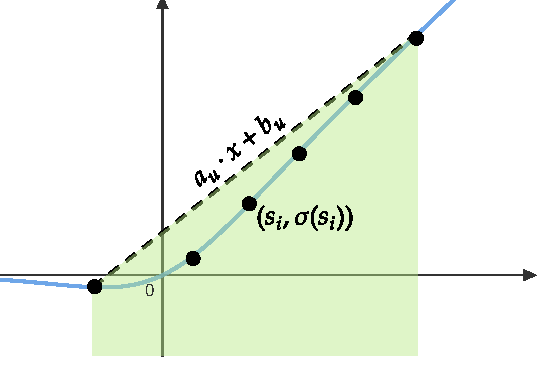
\includegraphics[width=0.5\linewidth]{offlinesyn/figs/sampling-lp.pdf}
	\caption{Illustration of the sampling and linear programming procedure for
	computing an upper bound. Shaded green region illustrates the volume below
	the upper bound.\label{offlinesyn:fig:samplelp}}
\end{figure}
%\end{wrapfigure}

\subsubsection{Generating Example Coefficients $ a_u, b_u $}
Given a fixed $ [l, u] $, we aim to generate upper bound coefficients $ a_u,
b_u $. A good generation procedure has three criteria: (1) the coefficients
should be tight for the input interval $ [l, u] $, (2) the coefficients should
be sound, and (3)
the generation should be fast. The first two criteria are intuitive: good training examples
will result in a good learned model. The third is to ensure that we can
generate a large number of examples in a reasonable amount of time.
Unfortunately, the second and third criteria are at odds, because proving
soundness is inherently expensive. To ensure a reasonable runtime, we relax the
second criteria to \textit{probably} sound. Thus our final goal is to minimize
volume below $ a_u, b_u $ such that $ \sigma(x) \leq a_u\cdot x + b_u $
\textit{probably} holds for $ x \in [l, u] $.

Our approach is inspired by a prior
work~\cite{ryou2021scalable,balunovic2019certifying}, which formulates the goal of a non-linear optimization problem
as a linear program that can be solved efficiently. Our approach samples points
$ (s_i, \sigma(s_i)) $ on the activation function for  $ s_i \in [l, u] $,
which are used to to convert the nonlinear constraint $ \sigma(x) \leq a_u\cdot
x + b_u $ into a linear one, and then uses volume as the objective (which is
linear). For a set $ S $ of sample points $ s_i \in [l, u] $, the
linear program we solve is:
\begin{gather*}
	\mathrm{minimize:} \; \mathrm{volume \;below}\;\; a_u\cdot x + b_u \\
	\mathrm{subj.\; to:} \;\; \bigwedge_{s_i \in S}
	\sigma(s_i) \leq a_u\cdot s_i + b_u
\end{gather*}
We illustrate this in Figure~\ref{offlinesyn:fig:samplelp}.
Solving the above problem results in $ a_u, b_u $, and the prior
work~\cite{ryou2021scalable,balunovic2019certifying} proved that the solution
(theoretically) approaches the optimal and sound $ a_u, b_u $ as the number of
samples goes to infinity. We use Gurobi~\cite{gurobi} to solve the linear
program.

\subsubsection{Converting $ a_u, b_u $ to a Tangent Line}
To use the generated $ a_u, b_u $ in the tangent-line form template,
we must find a point $ t $ whose tangent line is close to $ a_u, b_u $.
That is, we require that the following condition (almost) holds:
\begin{gather*}
	(\sigma'(t) = a_u) \wedge (\sigma'(t)\cdot t + \sigma(t) = b_u)
\end{gather*}
To solve the above problem, we use local optimization techniques (specifically a
modified Powell's method~\cite{powell1964efficient} implemented in
SciPy~\cite{2020SciPy-NMeth}, but most common techniques would work) to find a
solution to $ \sigma'(t) = a_u $.


We then check that the right side of the above formula almost holds
(specifically, we check ($ |(\sigma'(t)\cdot t + \sigma(t)) - b_u
| \leq 0.01 $). If the local optimization does not converge (i.e., it
does not find a $ t $ such that $ \sigma'(t) = a_u $), or the check on
$ b_u $ fails, we throw away the example and do not use it in
training.
\begin{figure}[t]
	\centering
	\begin{minipage}{.48\linewidth}
		\centering
		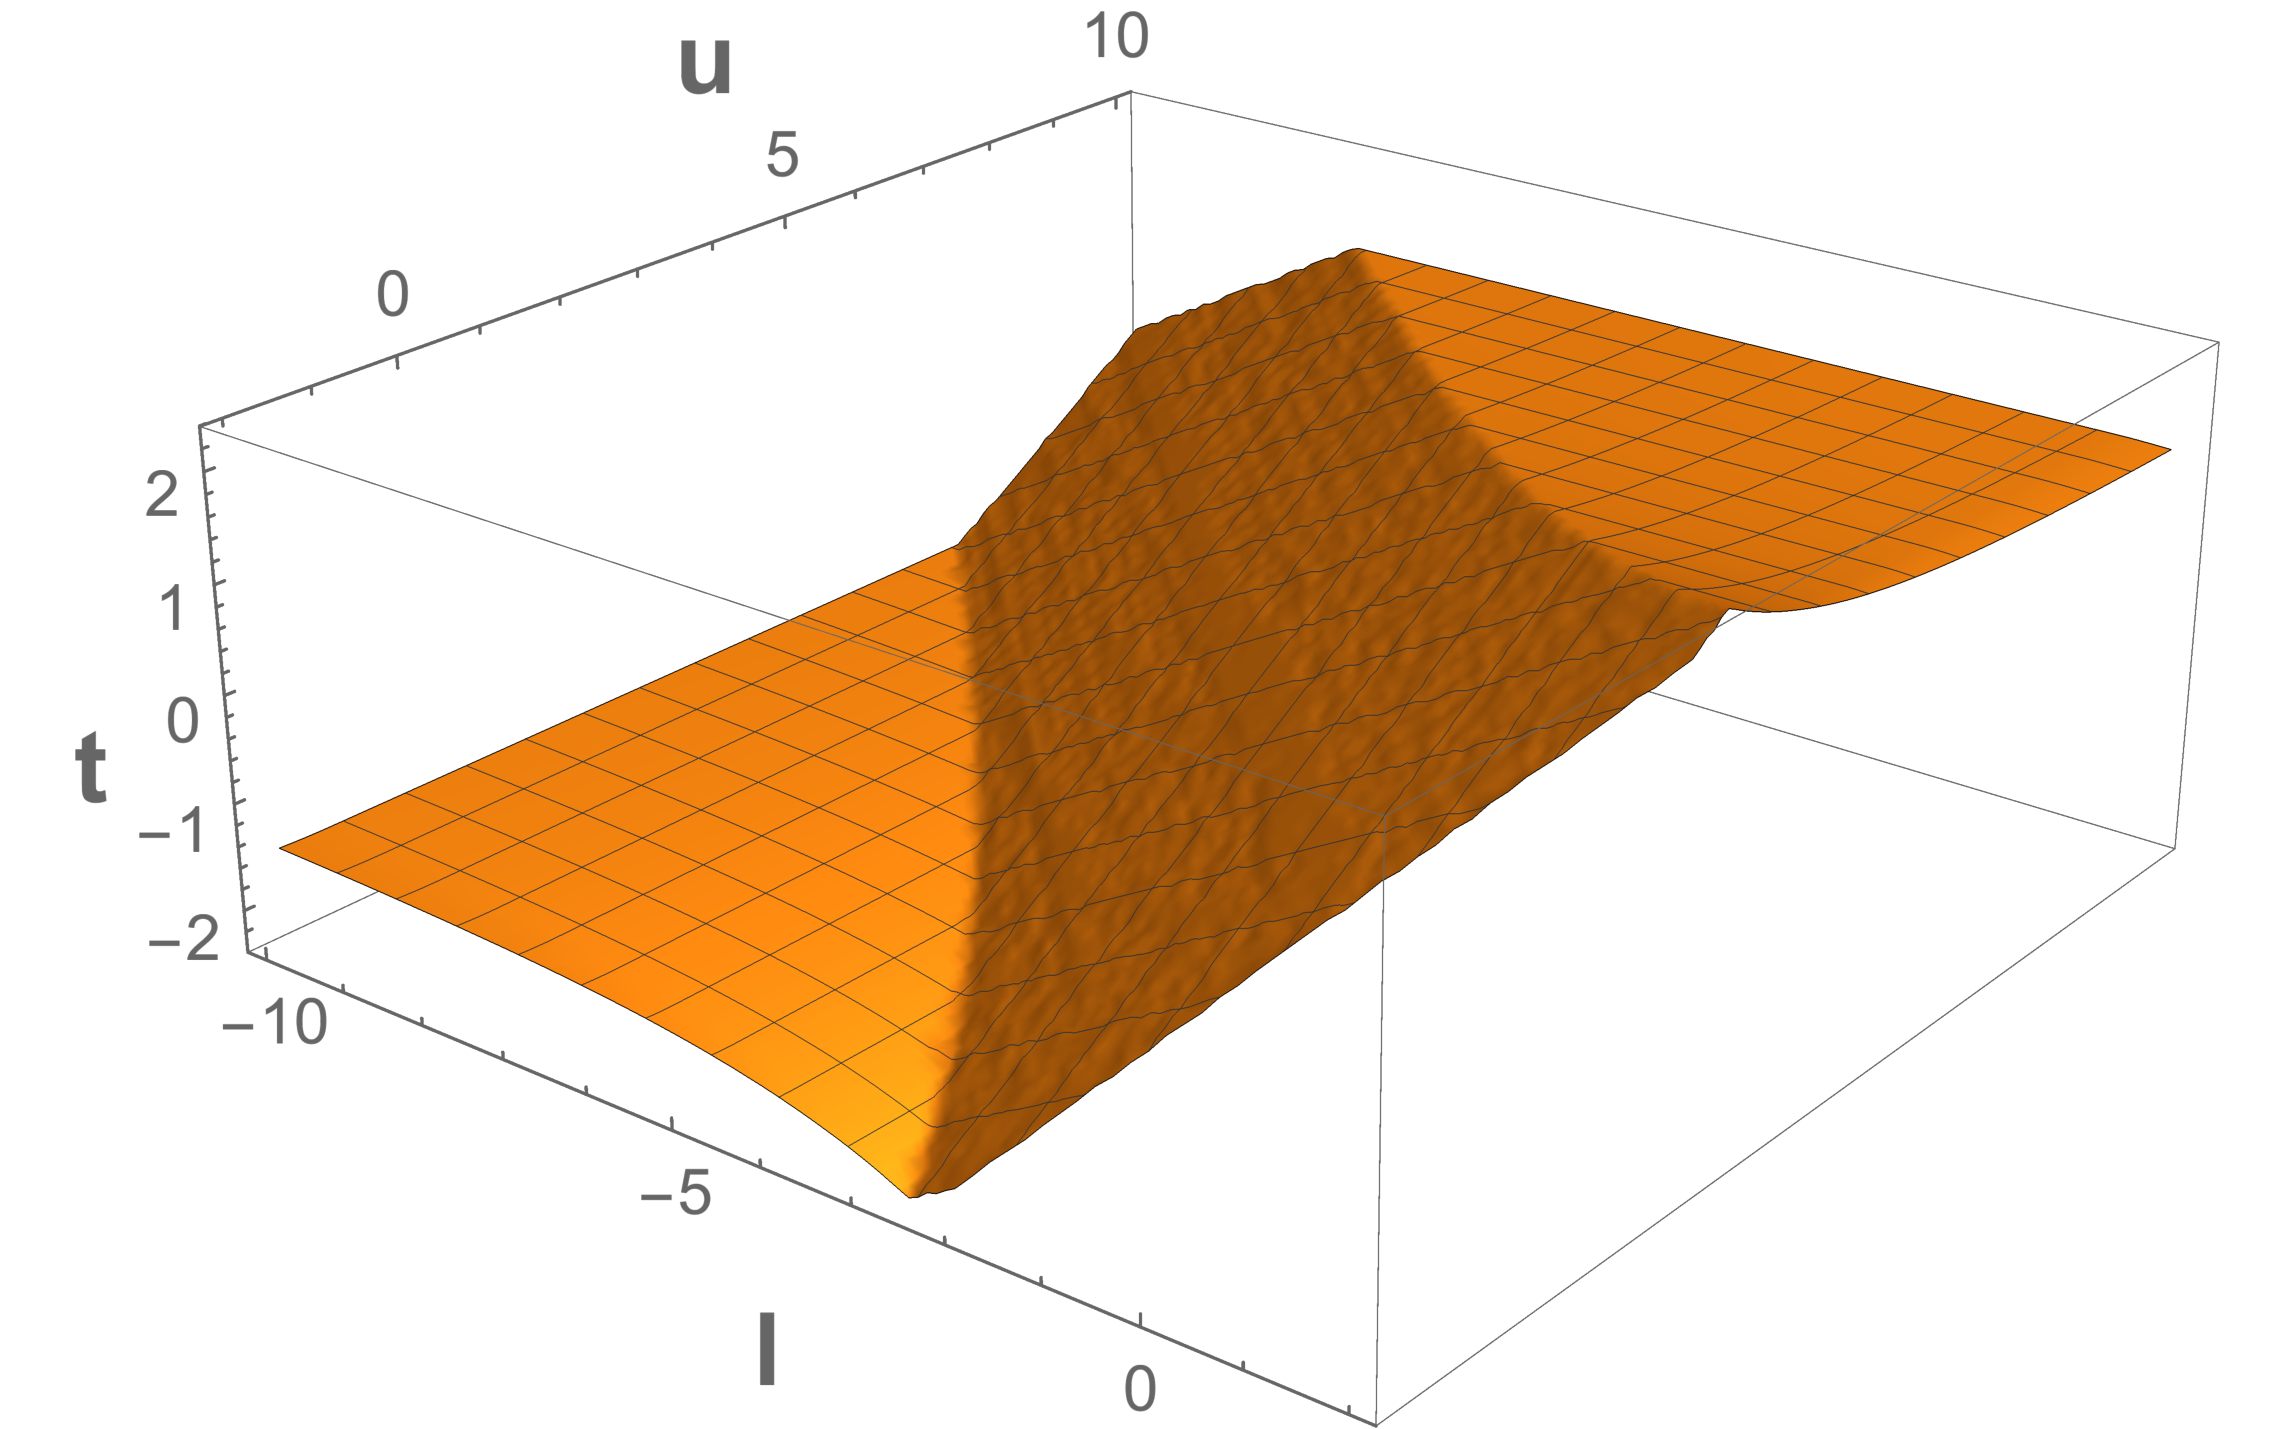
\includegraphics[width=\linewidth]{offlinesyn/figs/tanplot.pdf}
	\end{minipage}\hspace{12pt}%
	\begin{minipage}{.48\linewidth}
		\centering
		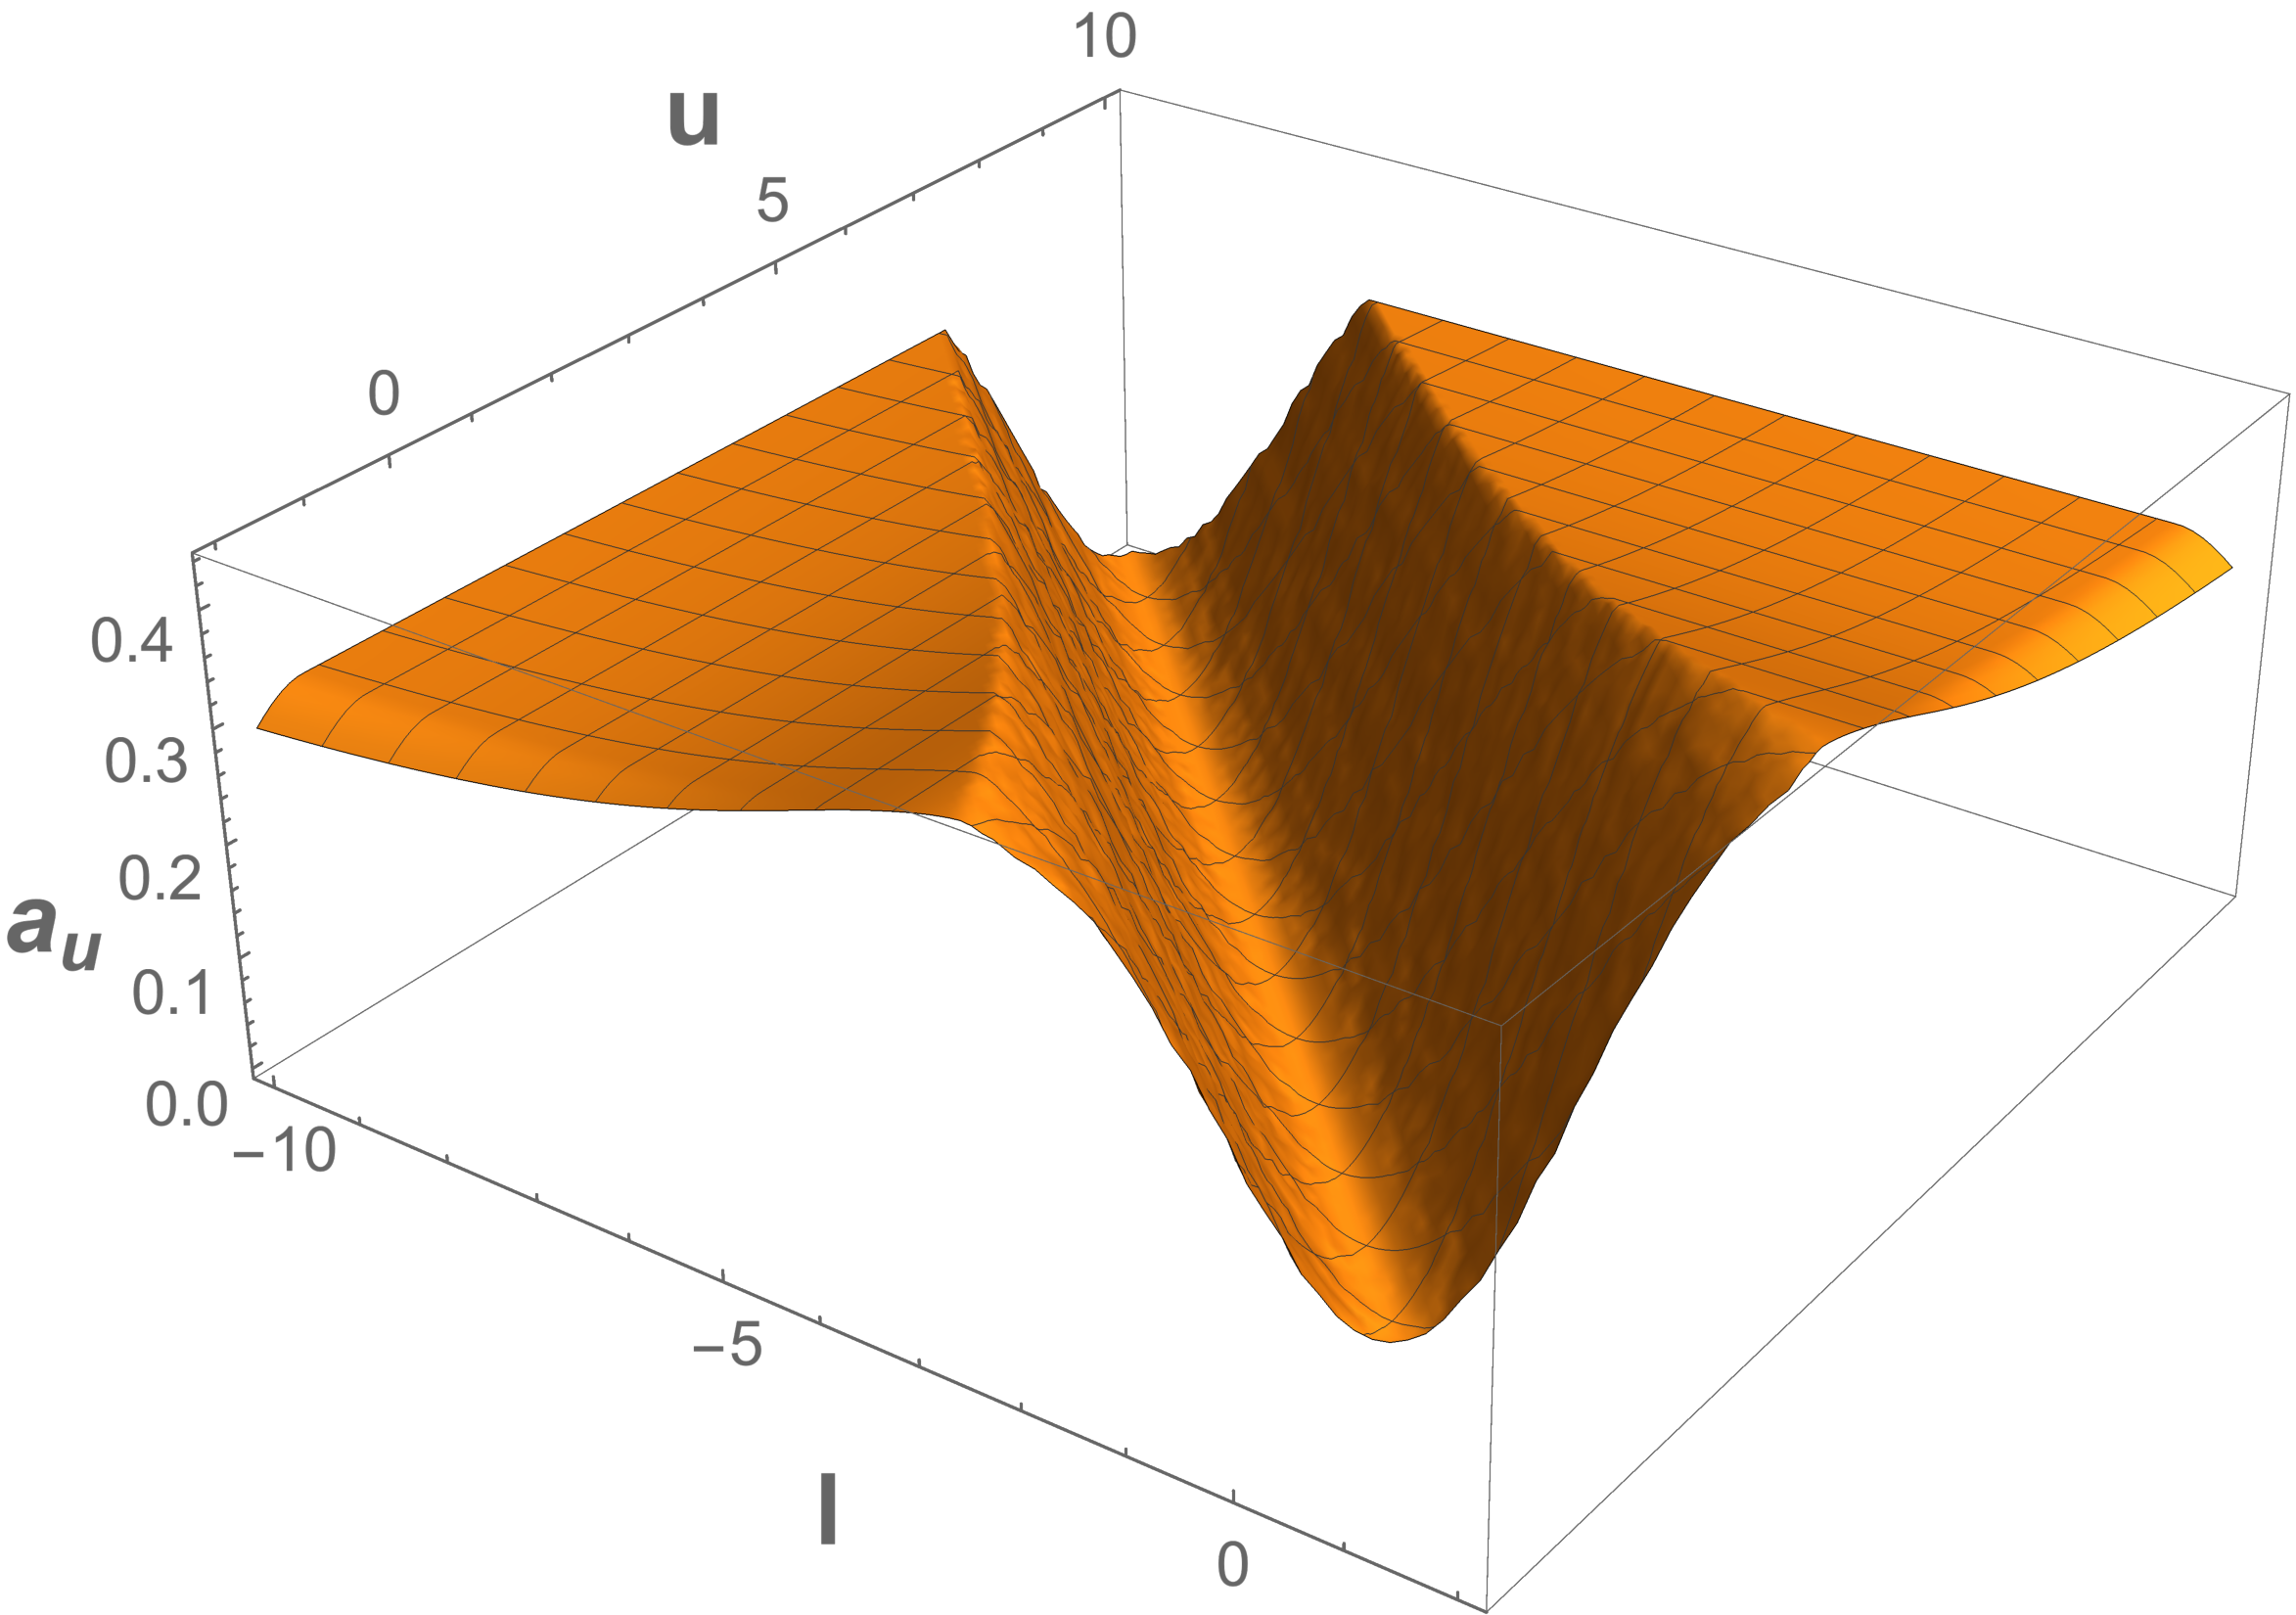
\includegraphics[width=\linewidth]{offlinesyn/figs/aplot.pdf}
	\end{minipage}
	\caption{Plots of the training examples, smoothed with linear
	interpolation. On the left: a plot of $ ((l, u), (t)) $, and on the right:
	a plot of $ ((l, u), (a_u)). $\label{offlinesyn:fig:targetfunc}}
	\label{offlinesyn:fig:funcstolearn}
\end{figure}

One may ask the question: could we simply train a model to directly predict the
coefficients $ a_u $ and $ b_u $, instead of predicting a tangent point and
then converting it to the tangent line? The answer is yes, however this
approach has two caveats. The first caveat is that we will lose the inherent
tightness that we gain with the tangent-line form -- we no longer have a
guarantee that the computed linear bound will touch $ \sigma(x) $ at
any point. The second caveat is  that the relationship between $ l, u $ and $ t $
tends to be close to linear, and thus easier to learn, whereas the relationship
between $ l, u$ and  $a_u $, or between $ l, u$ and $ b_u $,  is highly nonlinear.
We illustrate these
relationships as plots in Figure~\ref{offlinesyn:fig:targetfunc}. The left graph
plots the
generated training examples $ ((l, u), t) $, converted to a smooth function
using linear interpolation. We can see most regions are linear, as shown by the
flat sections. The right plot shows $ ((l, u), a_u) $, where we can see
the center region is highly nonlinear.

\subsubsection{Training on the Examples}
% TODO: Need ALGORITHMS!!!!!
Using the procedure presented so far, we sample $ [l, u] $ uniformly from $
I_{i,j} $ and generate the corresponding $ t $ for each of them. This results
in a training dataset of $ r $ examples $ \mathcal{D}_{train} = \{ ((l_i, u_i),
t_i) ~|~ i \in \{1..r\} \} $. We then choose between one of two models -- a
linear regression model or a 2-layer, 50-hidden-neuron, ReLU network -- to become
the final function $ g(l, u) $. To decide, we train both model types, and choose the one
with the lowest error, where error is measured as the mean absolute error. We give
details below.

A linear regression model is a function $ g(l, u) = c_1 \cdot l +
c_2 \cdot u + c_3 $, where $ c_i \in \mathbb{R} $ are coefficients
learned by minimizing the \textit{squared error}, which formally is:
\begin{equation}\label{offlinesyn:eq:sqerror}
	\sum_{((l_i, u_i), t_i) \in D_{train}} (g(l_i, u_i) - t_i)^2
\end{equation}
Finding the coefficients $ c_i $ that minimize the above constraint has a closed-form
solution, thus convergence is guaranteed and optimal, which is desirable.

However, sometimes the relationship between $ (l, u) $ and $ t $ is nonlinear,
and thus using a linear regression model may result in a poor-performing $ g(l,
u) $, even though the solution is optimal. To capture more complex
relationships, we also consider a 2-layer ReLU network where $
\mathbf{W}_0 \in \mathbb{R}^{2\times50} $, $ \mathbf{W}_1 \in
\mathbb{R}^{50\times1} $, $ \mathbf{b}_0 \in \mathbb{R}^{50} $, $ \mathbf{b}_1
\in \mathbb{R} $, and we have $ g(l, u) = \text{ReLU}(\langle l,u \rangle^T
\cdot \mathbf{W}_0 + \mathbf{b}_0) \cdot \mathbf{W}_1 + \mathbf{b}_1 $. The
weights and biases are initialized randomly, and then we minimize the
squared error (Equation~\ref{offlinesyn:eq:sqerror}) using gradient
descent. While convergence to the optimal weights is not guaranteed in
theory, we find in practice it usually converges.

We choose these two models because they can capture a diverse set of $ g(l , u) $ functions. While
we could use other prediction models, such as polynomial regression, generally, a neural
network will be equally (if not more) expressive. However, we believe exploring
other model types or architectures of neural networks would be an interesting
direction to explore.

%\textcolor{red}{Need to explain, in more detail,  how ``vanilla machine
%learning models'' are actually used.  I am sure people what to know more about
%this -- merely saying vanilla machine learning model is not good enough.  For
%example, was it a linear regression, or a low-degree polynomial regression,
%and
%what does the neural network look like, and what ``small'' really means?}


\subsection{Ensuring Soundness of the Linear
Approximations}\label{offlinesyn:sec:soundness}
For a given $ I_{i, j} $, we must ensure that its corresponding coefficient
generator functions $ \mathcal{G}_{a_u}(l ,u)$ and $ \mathcal{G}_{b_u}(l ,u) $
are sound, or in other
words, that the following condition does \textbf{not} hold:
\begin{gather*}\label{offlinesyn:eq:sound-opt}
\exists [l, u] \in I_{i, j}, \; x \in [l, u] ~.~
\sigma(x) > \mathcal{G}_{a_u}(l, u)\cdot x + \mathcal{G}_{b_u}(l, u)
\end{gather*}
We ensure the above condition does not hold (the formula is unsatisfiable) by bounding the \textit{maximum violation} on
the clause $ \sigma(x) > \mathcal{G}_{a_u}(l, u)\cdot x + \mathcal{G}_{b_u}(l,
u) $,
which we formally define as
$ \Delta(l, u, x) =  \sigma(x) - (\mathcal{G}_{a_u}(l, u)\cdot x +
\mathcal{G}_{b_u}(l, u)) $. $ \Delta $ is
positive when the previous clause holds.  Thus, if we can compute an upper bound
$ \Delta_u $, we can set the $ \epsilon $ term in $ \mathcal{G}_{b_u}(l, u) $
to $ \Delta_u $
to ensure the clause does not hold, thus making the coefficient generator functions sound.

To compute $ \Delta_u $, we solve (i.e., bound) the following optimization
problem:
\begin{gather*}\label{offlinesyn:eq:opt}
\mathrm{for:}\;\; l, u, x \in [l_{i,j}, u_{i,j}] \\
\mathrm{maximize:}\;\; \Delta(l, u, x)\\
\mathrm{subj. \; to:}\;\;
l < u \wedge l \leq x \wedge x \leq u
\end{gather*}
where $ l_{i,j}, u_{i,j} $ are the minimum lower bound and maximum upper bound,
respectively, for any interval in $ I_{i, j} $.
The above problem can be solved using the general framework of interval
analysis~\cite{moore2009introduction} and branch-and-prune
algorithms~\cite{benhamou2006continuous}.

Letting
$ \Delta_{search} = \{(l, u, x) | l, u, x \in [l_{i,j}, u_{i,j}] \} $
be the domain over which we want to bound $ \Delta $,
we can bound $ \Delta $ over $ \Delta_{search} $ using interval analysis.
%
In
addition, we can improve the bound in two ways: \textit{branching} (i.e.,
partitioning $ \Delta_{search} $ and bounding $ \Delta $ on each subset
separately) and \textit{pruning} (i.e., removing from $ \Delta_{search} $
values that violate the constraints $ l < u \wedge l \leq x \wedge x \leq u $).
The tool IbexOpt~\cite{chabert2009contractor} implements such an algorithm, and
we use it solve the above optimization problem.

One practical consideration when solving the above optimization problem is the
presence of division by zero error. In the two-point template, we have
$ \mathcal{G}_{a_u}(l, u) = \frac{\sigma(u) - \sigma(l)}{u - l} $. While we
have the
constraint $ l < u $, from an interval analysis perspective, $
\mathcal{G}_{a_u}(l, u) $ goes
to infinity as $ u - l $ goes to 0, and indeed, if we gave the above problem to
IbexOpt, it would report that $ \Delta $ is unbounded. To account for this, we
enforce a minimum interval width of $ 0.01 $ by changing $ l < u $ to $ 0.01 <
u - l $.

%\begin{figure}[t]
%	\centering
%	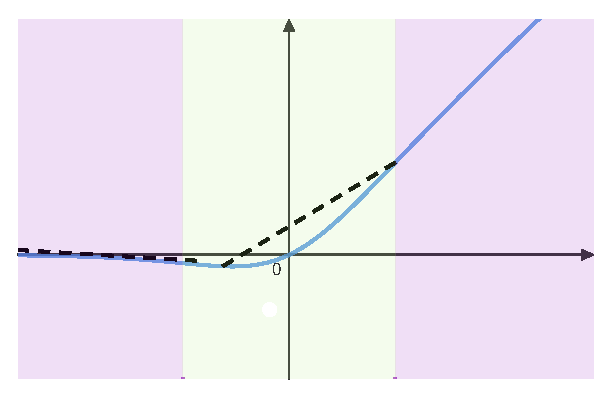
\includegraphics[width=0.5\linewidth]{offlinesyn/figs/convex.pdf}
%	\caption{An illustration of the convex (green) and concave (purple) regions
%	of Swish, and two linear upper bounds.\label{offlinesyn:fig:convex}}
%\end{figure}
%\subsubsection{Exploiting Convex and Concave Regions}
%Another advantage of structuring our templates as two-point and tangent-point
%templates is that they allow us to exploit the convex ($ \cup $-shaped) and
%concave ($ \cap $-shaped) regions of $ \sigma(x) $. Formally, we denote by $
%[l_i^\cup, u_i^\cup] $ an interval over which $ \sigma(x) $ is convex (there
%may be several, hence the $ i $), and $ [l_i^\cap, u_i^\cap] $ a concave
%region. We defer discussing how to obtain these intervals until the end of this
%subsection. In Figure~\ref{offlinesyn:fig:convex}, we illustrate the convex and
%concave
%regions of Swish.
%
%For the two-point template, we can exploit the convex regions. For a convex
%interval $ [l_i^\cup, u_i^\cup] $, the two-point form for any interval $ [l, u]
%\subseteq [l_i^\cup, u_i^\cup] $ is guaranteed to be a sound
%upper bound (this follows from the definition of convexity). We illustrate such
%a two-point form bound in Figure~\ref{offlinesyn:fig:convex} in the shaded green
%region.
%We can exploit this to skip verification for some two-point form $ I_{i, j} $.
%Formally, let $ I_\cup = \bigcup_i [l_i^\cup, u_i^\cup] \times [l_i^\cup,
%u_i^\cup] $ be the set of all intervals contained in a convex region. If we
%have $ I_{i, j} \ I_\cup = \emptyset $, then we can skip the verification of $
%I_{i,j} $'s template all together (i.e. set $ \epsilon = 0 $).
%
%In addition, we can exploit concave regions to partially or
%completely verify a tangent-point template. Concave regions have the following
%property: given a concave interval $ [l_i^\cap, u_i^\cap] $,
%a line tangent to $ \sigma(x) $ at point $ t \in [l_i^\cap, u_i^\cap] $ must
%be entirely above $ \sigma(x) $ over the interval $ [l_i^\cap, u_i^\cap] $
%(this follows the from the definition of concavity). We illustrate such a
%tangent line in the shaded purple region in Figure~\ref{offlinesyn:fig:convex}.
%To verify
%soundness of this tangent line, we would only need to look for violations
%outside the purple shaded region.
%
%However, we cannot directly exploit concavity without modifying our
%tangent-point template. In order to exploit it, we must ensure that, for some
%fixed concave region $ [l_i^\cap, u_i^\cap] $, $  g(l, u) \in [l_i^\cap,
%u_i^\cap] $ for all $ [l, u] \in I_{i,j} $. If we can ensure this, then we
%modify the domain of the variable $ x $ in the optimization problem in
%Equation~\ref{offlinesyn:eq:opt} to be $ x \in [l_{i,j}, u_{i,j}] \ [l_i^\cap,
%u_i^\cap] $ because there cannot be any violations of
%Equation~\ref{offlinesyn:eq:sound-opt} for $ x \in [l_i^\cap, u_i^\cap] $. This
%reduction
%in domain greatly speeds up solving Equation~\ref{offlinesyn:eq:opt}.
%
%To choose the appropriate $ [l_i^\cap, u_i^\cap] $ for a given $ I_{i, j} $, we
%use the training examples $ D_{train} $ described in
%Section~\ref{offlinesyn:sec:learning}.
%
%
%\textit{Finding Convex/Concave Intervals}
%We take a very simple sampling approach for finding the convex and concave
%intervals, and we omit a full discussion. At a high-level, we sample points on
%the second derivative $ \sigma''(x) $ to find intervals where it is always
%positive and always negative. We then verify that these intervals are indeed
%convex/concave by using Ibex~\cite{chabert2009contractor} to prove $ \forall x
%\in [l_i^\cup, u_i^\cup] ~.~ \sigma''(x) > 0 $.

%\subsubsection{Verifying the Two-Point Form Bounds}
%
%In this step, we are given $ I_{2pt} $, which is simply a list of $ n_{2pt} $
%boxes that we refer to simply as $ I_{k} $ for $ k \in \{1..n_{2pt}\} $. For
%each $ I_k $, we must verify:
%% TODO: put the proper bound on x
%\begin{gather*}
%\forall x, (l, u) \in I_k \\
%l \geq u \vee l > x \vee x > u \; \vee \\
%\sigma(x) \leq a_u(l, u)x + b_u(l, u)
%\end{gather*}
%
%% removing intervals that are entirely convex in a convex region
%Let $ I_\smile $ be the set of all intervals that are entirely contained in a
%convex region. We only need to verify the portion of $ I_k $ not in $ I_\smile
%$, i.e., $ I_k - I_\smile $.
%
%% optimizing verification of intervals that cross a
%
%\subsubsection{Verifying the Tangent Line Form Bounds}
%
%We restrict $ g(l, u) $ so that it is always in a concave region $ [ l_\frown,
%u_\frown ] $, so we can always prune the concave region from the search space.

\subsection{Efficient Lookup of the Linear Bounds}

Due to partitioning $ I_x $, we must have a procedure for looking up the
appropriate template instance for a given $ [l, u] $ at the application time.
Formally, we need to find the box
$ I_{i, j} $, which we denote $ [l_l, u_l] \times [l_u, u_u] $,
such that $ l \in [l_l, u_l] $ and $ u \in [l_u, u_u] $, and retrieve the
corresponding template. Lookup can actually present a significant runtime overhead if
not done with care. One approach is to use a data structure similar to an interval
tree or a quadtree~\cite{finkel1974quad}, the latter of which has $
\mathcal{O}(log(n)) $ complexity. While the quadtree would be the most
efficient for an arbitrary partition of $ I_x $ into boxes, we can in fact
obtain $ \mathcal{O}(1) $ lookup for our partition strategy.

We first note that each box, $ I_{i, j} $,
can be uniquely identified by $ l_l $ and $ u_u $. The point $ (l_l, u_u) $
corresponds to the top-left corner of a box in
Figure~\ref{offlinesyn:fig:partition}.
%
Thus we build a lookup dictionary keyed by $ (l_l, u_u) $ for each box that
maps to the corresponding linear bound template.
%
To perform lookup, we exploit the structure of the partition: specifically,
each box in the partition is aligned to a multiple of $ c_s $.
%
Thus, to lookup $ I_{i,j} $ for a given $ [l, u] $, we view $ (l, u) $ as a
point on the graph of Figure~\ref{offlinesyn:fig:partition}, and the lookup
corresponds to
moving left-ward and upward from the point $ (l, u) $ to the nearest upper-left
corner of a box.
%
More formally, we perform lookup by rounding $ l $ down to the nearest
multiple of $ c_s $, and $ u $ upward to the nearest multiple of $ c_s $.
The top-left corner can then be used to lookup the appropriate template.


%\begin{itemize}
%	\item min width to ensure efficiency of bounding max viol of two point form
%	(there could be a zero denom if we don't have a min width)
%	\item what if we encounter $ [l, u] $ at runtime that is out of the $ l_x,
%	u_x $ range? we fall back to IBP
%	\item efficient lookup
%\end{itemize}

\section{Evaluation}
\label{offlinesyn:sec:experiment}

We have implemented our approach as a software tool that synthesizes a linear
bound generator function $ \mathcal{G}(l,u) $ for any given activation function
$ \sigma(x) $ in the input universe $ x \in
[l_x, u_x] $. The output is a function that takes as input $ [l, u] $ and
returns
coefficients $ a_l, b_l, a_u, b_u $ as output. For all experiments, we use $ l_x = -10,
u_x = 10 $, $ c_s = 0.25 $, and a minimum interval width of $ 0.01 $.
%
After the generator function is synthesized, we integrate it into
\autolipra{}, a state-of-the-art neural network verification tool, which allows us to analyze neural networks
with $ \sigma(x) $ as activation functions.

\subsection{Benchmarks}


\subsubsection{Neural Networks and Datasets}
Our benchmarks are eight deep neural networks trained on the following two
datasets.

\textit{MNIST}. MNIST~\cite{LecunBBH98} is a set of images of hand-written
digits
each of which are labeled with the corresponding written digit. The images are
28x28 grayscale images with one of ten written digits. We use a convolutional
network architecture with 1568, 784, and 256 neurons in its first, second, and
third layer, respectively. We train a model for each of the activation
functions described below.

\textit{CIFAR}. CIFAR~\cite{krizhevsky2009learning} is a set of images
depicting one of 10
objects (a dog, a truck, etc.), which are hand labeled with the
corresponding object. The images are 32x32 pixel RGB images. We use a
convolutional architecture with 2048, 2048, 1024, and 256 neurons in the first,
second, third, and fourth layers, respectively. We train a model for each of
the activation functions described below.

\subsubsection{Activation Functions}
Our neural networks use one of the activation functions shown
Figure~\ref{offlinesyn:fig:acts} and defined in Table~\ref{offlinesyn:tbl:acts}.
They are
Swish~\cite{hendrycks2016gaussian,ramachandran2017searching},
GELU~\cite{hendrycks2016gaussian}, Mish~\cite{misra2019mish},
LiSHT~\cite{roy2019lisht}, and AtanSq~\cite{ramachandran2017searching}. The
first two are used in language models such as
GPT~\cite{radford2018improving}, and have been shown to achieve
the best performance for some image classification
tasks~\cite{ramachandran2017searching}. The third and fourth two are variants
of the first two, which are shown to have desirable theoretical properties. The
last was discovered using automatic search
techniques~\cite{ramachandran2017searching}, and found to perform on par with
the state-of-the-art. We chose these activations because they are representative of
recent developments in deep learning research.

\begin{figure}[t]
	\centering
	\begin{minipage}{.48\textwidth}
		\centering
		\begin{table}[H]
			\caption{Definitions of activation functions used in our experiments.}
			\scalebox{0.86}{%
				\renewcommand{\arraystretch}{1.2}
				\begin{tabular}{|l|l|}
					\hline
					Name  &
					Definition
					\\
					\hline
					Swish & $x \cdot
					sigmoid(x)$                                              \\
					\hline
					GELU  & $ 0.5 x ( 1 + \tanh{[ \sqrt{2 / \pi } (x + 0.044715x
						^{3} ) ] } )$ \\ \hline
					Mish  & $x \cdot \tanh{[\text{ln}( 1 + e^x
						)]}$                                    \\ \hline
					LiSHT & $x \cdot
					\tanh{(x)}$
					\\
					\hline
					AtanSq & $ (\text{tan}^{-1}(x))^2  - x $ \\ \hline
				\end{tabular}}
			\label{offlinesyn:tbl:acts}
		\end{table}
	\end{minipage}\hspace{12pt}%
	\begin{minipage}{.48\textwidth}
		\centering
		\scalebox{1.1}{
			\begin{tikzpicture}
        \begin{axis}[
            xmin = -5, xmax = 3,
            ymin = -1.2, ymax = 3.5,
            xtick distance = 10,
            ytick distance = 10,
            %grid = both,
            %minor tick num = 1,
            %major grid style = {lightgray},
            %minor grid style = {lightgray!25},
            width = \linewidth,
            height = 0.75\linewidth,
            xticklabel=\empty,yticklabel=\empty,
            minor tick num=0,
%            major tick num=0,
%            hide axis,
            axis lines = middle,
            legend cell align = {left},
%            legend pos = north west,
			set layers=standard,
	        legend to name=grouplegend,
	        legend entries={{Swish},
	        	{LiSHT},
	        	{Mish},
	        	{GELU},
        		{AtanSq},},
        	legend style={nodes={scale=0.9, transform shape},font=\scriptsize,
        	draw=none,fill=white,align=left},
        ]
			\addplot[actfunc, blue] {x * (1 / (1 + exp(-x)))};
            \addplot[actfunc, green,domain=-3:3] {x * tanh(x)};
            \addplot[actfunc, purple] {x * tanh(ln(1+exp(x)))};
            \addplot[actfunc, cyan] {0.5*x * ( 1 + tanh(sqrt(2/pi) * (x+
            0.044715 * (x ^3) ) ) )};
            \addplot[actfunc, purple, domain=-2:2.5] {rad(atan(x))^2 - x};
			\coordinate (leg) at (rel axis cs:-0.15,0.95);

%            \legend{
%             {$ 0.5 x ( 1 + \tanh{ \sqrt{2 / \pi } (x + 0.044715 x ^{3} ) } ) $
%              \\ (GeLU)},
%             {$ min(1, max(x, -1)) $ (Hard Tanh)},
%             $ 1 - e^{-e^{x}} $ (Log-Log),
%    	     $ x * \sigma(x) $ (Swish),
%                }
        \end{axis}
        \node[anchor= north west] at
        (leg){\pgfplotslegendfromname{grouplegend}};
\end{tikzpicture}
}
		\caption{Activation functions used in our experiments.}
		\label{offlinesyn:fig:acts}
	\end{minipage}
\end{figure}

\subsubsection{Robustness Verification}
% TODO: $\epsilon$ is used already!
We evaluate our approach on \textit{robustness} verification problems. Given a
neural network $ f: \mathbb{X} \subseteq \mathbb{R}^n \to \mathbb{Y} \subseteq
\mathbb{R}^m $ and an input $ \mathbf{x} \in \mathbb{X} $, we verify robustness
by proving that making a small $ p $-bounded perturbation ($ p \in \mathbb{R}
$) to $ \mathbf{x} $ does not change the classification. Letting $
\mathbf{x}[i] \in \mathbb{R} $ be the $ i^{th} $ element in $ \mathbf{x} $, we
represent the set of all perturbations as $ X \in \mathbb{IR}^n $, where $ X =
\bigtimes_{i=1}^n [\mathbf{x}[i] - p, \mathbf{x}[i] + p] $. We then compute $ Y
\in \mathbb{IR}^m $ where $ Y = \bigtimes_{i=1}^m [l_i,
u_i] $, and, assuming the target class of $ \mathbf{x} $ is $ j $, where $ j \in
\{1..m\} $, we prove robustness by checking $ (l_j > u_i)$ for all $i \neq j$ and $i \in
\{1..m\} $.

For each network, we take 100 random test images, and following prior
work~\cite{GehrMDTCV18}, we filter out misclassified images. We then take
the remaining images, and create a robustness verification problem for each
one. Again following prior work, we use $ p = 8/255 $ for MNIST networks
and $ p = 1/255 $ for CIFAR networks.

\subsection{Experimental Results}

Our experiments were designed to answer the following question: How do our
synthesized linear approximations compare with other state-of-the-art,
hand-crafted linear approximation techniques on novel activation functions?
%
To the best of our
knowledge,~\autolipra{}~\cite{autolipra} is the only neural network
verification tool capable of handling the activation functions we considered here
using static, hand-crafted approximations.
%
We primarily focus on comparing the number of verification problems solved
%
and we caution against directly comparing the runtime of our approach
against~\autolipra{}, as the latter is highly engineered for parallel computation,
whereas our approach is not currently engineered to take advantage of parallel computation (although it
could be).
%
We conducted all experiments on an 8-core 2.7GHz processor with 32GB of RAM.
\footnotetext[1]{\autolipra{} does not have an approximation for $
	\text{tan}^{-1} $.}
%
%\textcolor{red}{We only have one result able (using synthesized bounds for
%verification). Is it possible to show some statistics about the synthesis
%part?
%For example, during synthesis, what's the percentage boxes in
%$|I_{2pt}|/|I_x|$
%vs.  $|I_{tan}|/|I_x|$? How many boxes use linear regression and how many use
%ReLU network to store the $g(l,u)$? How many boxes failed the soundness
%verification and thus needed to be shifted by $$?  And in general, how
%much time was spent on each step of the synthesis procedure?}


We present results on robustness verification problems in
Table~\ref{offlinesyn:tbl:1}.
The first column shows the dataset and architecture. The next two columns show
the percentage of the total number of verification problems solved (i.e.,
robustness proved) and the total runtime in seconds for~\autolipra{}. The next
two columns show the same statistics for our approach. The final column
compares the
output set sizes of~\autolipra{} and our approach. We first define $ |Y| $ as
the volume of the (hyper)box $ Y $. Then letting $ Y_{auto} $ and $ Y_{ours} $
be the output set computed by~\autolipra{} and our approach, respectively, $
\frac{|Y_{ours}|}{|Y_{auto}|} $ measures the reduction in output set size. In
general, $ |Y_{ours} | < | Y_{auto} | $ indicates our approach is better
because it implies that our approach has more accurately approximated the true
output set, and thus $ \frac{|Y_{ours}|}{|Y_{auto}|} < 1 $ indicates our
approach is more accurate.


\begin{table}[t]
	\centering
	\caption{Comparison of the verification results of our approach and \autolipra{}.}
	\label{offlinesyn:tbl:1}
	\scalebox{0.9}{
		\renewcommand{\arraystretch}{1.15}

		\begin{tabular}{|ll|cr|cr|c|}
			\hline
			& \multicolumn{1}{c|}{\multirow{2}{*}{Network Architecture}} &
			\multicolumn{2}{l|}{AutoLiPRA~\cite{autolipra}}               &
			\multicolumn{2}{l|}{Our Approach }                           &
			\multirow{2}{*}{\ \ $ \frac{|Y_{ours}|}{|Y_{auto}|}$\ \ } \\ \cline{3-6}
			& \multicolumn{1}{c|}{}                                      &
			\multicolumn{1}{c|}{\% certified} & time (s) &
			\multicolumn{1}{l|}{\% certified} & \multicolumn{1}{l|}{time (s)}
			&                                                   \\ \hline \hline
			\multicolumn{1}{|l|}{MNIST} & 4-Layer CNN with
			Swish                                     &
			\multicolumn{1}{c|}{0.34}         & 15       &
			\multicolumn{1}{c|}{0.74}         & 195                           &
			0.59                                              \\ \cline{2-7}
			\multicolumn{1}{|l|}{}      & 4-Layer CNN with
			Gelu                                      &
			\multicolumn{1}{c|}{0.01}         & 359      &
			\multicolumn{1}{c|}{0.70}          & 289                           &
			0.22                                              \\ \cline{2-7}
			\multicolumn{1}{|l|}{}      & 4-Layer CNN with
			Mish                                      &
			\multicolumn{1}{c|}{0.00}         & 50       &
			\multicolumn{1}{c|}{0.28}         & 236                           &
			0.29                                              \\ \cline{2-7}
			\multicolumn{1}{|l|}{}      & 4-Layer CNN with
			LiSHT                                     &
			\multicolumn{1}{c|}{0.00}          & 15       &
			\multicolumn{1}{c|}{0.11}          & 289                           &
			0.32                                              \\ \cline{2-7}
			\multicolumn{1}{|l|}{}      & 4-Layer CNN with
			AtanSq\footnotemark{}                                 &
			\multicolumn{1}{c|}{-}            & -        &
			\multicolumn{1}{c|}{0.16}         & 233                           &
			-                                                 \\ \hline \hline
			\multicolumn{1}{|l|}{CIFAR} & 5-Layer CNN with
			Swish                                     &
			\multicolumn{1}{c|}{0.03}         & 69       &
			\multicolumn{1}{c|}{0.35}         & 300                           &
			0.42                                              \\ \cline{2-7}
			\multicolumn{1}{|l|}{}      & 5-Layer CNN with
			Gelu                                      &
			\multicolumn{1}{c|}{0.00}         & 1,217    &
			\multicolumn{1}{c|}{0.29}          & 419                           &
			0.21                                              \\ \cline{2-7}
			\multicolumn{1}{|l|}{}      & 5-Layer CNN with
			Mish                                      &
			\multicolumn{1}{c|}{0.00}         & 202      &
			\multicolumn{1}{c|}{0.29}         & 363                           &
			0.17                                              \\ \cline{2-7}
			\multicolumn{1}{|l|}{}      & 5-Layer CNN with
			LiSHT                                     &
			\multicolumn{1}{c|}{0.00}         & 68       &
			\multicolumn{1}{c|}{0.00}          & 303                           &
			0.09                                              \\ \cline{2-7}
			\multicolumn{1}{|l|}{}      & 5-Layer CNN with
			AtanSq\footnotemark[1]{}                                    &
			\multicolumn{1}{c|}{-}            & -        &
			\multicolumn{1}{c|}{0.22}          & 347                           &
			-                                                 \\ \hline
		\end{tabular}
	}

\end{table}


We point out three trends in the results. First, our automatically synthesized
linear approximations always result in more verification problems solved. This
is because our approach synthesizes a linear approximation specifically for $
\sigma(x) $, which results in tighter bounds. Second,~\autolipra{} takes longer
on more complex activations such as GELU and Mish, which have more elementary
operations than Swish and LiSHT. This occurs because~\autolipra{} has more
linear approximations to compute (it must compute one for every elementary
operation before composing the results together). On the other hand, our
approach computes the linear approximation in one step, and thus does not have
the additional overhead for the more complex activation functions. Third, our
approach always computes a much smaller output set, in the range of 2-10X
smaller, which again is a reflection of the tighter linear bounds.
%\paragraph{Overall Comparison}

%\textcolor{red}{Need to say a few words about CIFAR -- LiSHT, for which our
%approach proved 0\% -- what's the reason for that?  Furthermore, is it
%possible
%that, although both methods proved 0\%,  our approach is still be better than
%\autolipra{} in some sense?}
\paragraph{Synthesis Results} We also report some key metrics about the
synthesis procedure. Results are shown in Table~\ref{offlinesyn:tbl:synth}. The
first
three columns show the total CPU time for the three steps in our synthesis procedure. We
note that all three steps can be heavily parallelized, thus the wall clock time
is roughly 1/8 the reported times on our 8-core machine. The final column shows
the percentage of boxes in the partition that were assigned a two-point
template (we can take the complement to get the percentage of tangent-line
templates).

%\begin{wrapfigure}{R}{0.5\textwidth}
\begin{table}[t]
	\centering
	\caption{Statistics of the synthesis step in our
	method.\label{offlinesyn:tbl:synth}}
	\scalebox{0.9}{
	\begin{tabular}{|l|r|r|r|c|}
		\hline
		Activation $\sigma(x)$ & \begin{tabular}[c]{@{}l@{}}Partition\ \ \ \\ Time
		(s)\end{tabular} & \begin{tabular}[c]{@{}l@{}}      Learning\ \ \ \ \ \\ Time
		(s)\end{tabular} & \begin{tabular}[c]{@{}l@{}}Verification\\ Time
		(s)\end{tabular} & \ \ \ \ $\frac{|I_{2pt}|}{|I_x|}$\ \ \ \  \\ \hline \hline
		Swish       &
		81                                                           &
		1,762                                                        &
		20,815                                                           &
		0.45                      \\ \hline
		GELU        &
		104                                                          &
		2,113                                                        &
		45,504                                                           &
		0.57                      \\ \hline
		Mish        &
		96                                                           &
		2,052                                                        &
		38,156                                                           &
		0.45                     \\ \hline
		LiSHT       &
		83                                                           &
		1,650                                                        &
		61,910                                                           &
		0.46                      \\ \hline
		AtanSq      &
		85                                                           &
		1,701                                                        &
		18,251                                                           &
		0.38                      \\ \hline
	\end{tabular}
}
\end{table}
%\end{wrapfigure}

\section{Related Work}
\label{offlinesyn:sec:related}

Most closely related to our work are those that leverage
interval-bounding techniques to conduct neural network verification.
Seminal works in this area can
either be thought of as explicit linear bounding, or linear bounding
with some type of restriction (usually for efficiency). Among the explicit
linear bounding techniques are the ones used in
~\DeepPoly{}~\cite{SinghGPV19},~\autolipra{}~\cite{autolipra},
~\Neurify{}~\cite{WangPWYJ18nips}, and
similar
tools~\cite{balunovic2019certifying,du2021cert,ko2019popqorn,zhang2018efficient,WengZCSHDBD18,wu2021tightening,ryou2021scalable,shi2020robustness}.
On the other hand,  techniques using Zonotopes~\cite{GehrMDTCV18,MirmanGV18} and
symbolic intervals~\cite{WangPWYJ18} can be thought of as restricted linear
bounding. Such approaches have an advantage in scalability, although they
may sacrifice completeness and accuracy. In addition, recent work leverages
semi-definite approximations~\cite{hu2020reach}, which allow for more
expressive, nonlinear lower and upper bounds. In addition, linear
approximations are used in nonlinear programming and
optimization~\cite{chabert2009contractor,trombettoni2011inner}.
However, to the best of our
knowledge, none of these prior works attempt to automate the process of crafting
the bound generator function $\mathcal{G}(l, u) $.


Less closely related are neural network verification approaches based
on solving systems of linear
constraints~\cite{KatzBDJK17,KatzHIJLLSTWZDK19,Ehlers17,HuangKWW17,BastaniILVNC16,HuangKWW17,baluta2019quantitative,tjeng2019evaluating}.
Such approaches typically only apply to networks with piece-wise-linear
activations such as ReLU and max pooling, for which there is little need to
automate any part of the verification algorithm's design (at least with respect
to the activation functions). They do not handle novel activation functions such as the ones concerned in our work.  These approaches have the advantage of being
complete, although they tend to be less scalable than interval analysis based
approaches.


Finally, we note that there are many works built off the initial linear approximation
approaches, thus highlighting the importance of designing tight and sound linear
approximations in general~\cite{Singh2019krelu,SinghGPV19iclr,WangPWYJ18nips,tran2019star,tran2020verification}.


%\paragraph{Future Work} An interesting line of future work would be
%to automatically synthesize other types of approximations, such as zonotopes
%or semi-definite
%relaxations. In addition, it is possible that approximations
%synthesized by our approach could be improved further, thus another line of
%future work
%would be \textit{refining} the approximations with additional training
%examples, or using counterexample guided techniques.


\section{Conclusions}
\label{offlinesyn:sec:conclusion}

We have presented the first method for statically
synthesizing a function that can generate tight and sound linear
approximations for neural network activation functions. Our approach
is example-guided, in that we first generate example linear
approximations, and then use these approximations to train a
prediction model for linear approximations at run time. We leverage
nonlinear global optimization techniques to ensure the soundness of
the synthesized approximations. Our evaluation on popular neural
network verification tasks shows that our approach significantly
outperforms state-of-the-art verification tools.

%%% chapter %%%%%%%%%%%%%%%%%%%%%%%%%%%%%%%%%%%%%%%%%%%%%%%%%%%%%%%%%%%%

% if you're "stapling" together papers, it's easy to include your paper
% directory by way of symlinks, or copying the entire paper as a
% subdirectory.
%
% for example, if your paper directory looks like the following:
%
%   foobar/          - top level paper directory
%   foobar/fig/      - where all graphics and figures live
%   foobar/paper.bib - bibliography
%   foobar/paper.tex - monolithic .tex file for paper
%
% then you might use the folloiwng:
%
%   \graphicspath{foobar/fig}
%   \addbibresource{foobar/paper.bib}
%   \documentclass[11pt]{report}
\usepackage[
  dissertation
 ,final
 ,raggedbottom
]{USCthesis}


% Brandon's packages
\usepackage{tikz}
\usepackage{pgfplots}
\pgfplotsset{compat=1.11}
\usepgfplotslibrary{groupplots}
\usetikzlibrary{decorations}
\usetikzlibrary{decorations.markings}
\usepgfplotslibrary{fillbetween}
\pgfplotsset{%
	actfunc/.style = {%
		domain=-5:3,
		samples = 400,
		smooth,
		thick,
		on layer={axis foreground},
	}
}

\usepackage{listings}
%\usepackage{amsmath}
\usepackage{mathtools}
\usepackage{xcolor}

\lstset{ %
	backgroundcolor=\color{white},   % choose the background color
	basicstyle=\footnotesize\ttfamily,        % size of fonts used for the
	%code
	columns=fullflexible,
	breaklines=true,                 % automatic line breaking only at
	%whitespace
	captionpos=b,                    % sets the caption-position to bottom
	tabsize=4,
	commentstyle=\color{mygreen},    % comment style
	escapeinside={\%*}{*)},          % if you want to add LaTeX within your
	%code
	keywordstyle=\color{blue},       % keyword style
	stringstyle=\color{mymauve}\ttfamily,     % string literal style
	frame=single,
	rulesepcolor=\color{red!20!green!20!blue!20},
	% identifierstyle=\color{red},
	language=c++,
	escapechar=!
}

\usepackage{comment}
\usepackage{algorithm2e}
\usepackage{amsthm}
\usepackage{multirow}
\usepackage{makecell}
\usepackage{amsmath}
\usepackage{float}

% Brandon's commands
\newcommand{\declarecommand}[1]{\providecommand{#1}{}\renewcommand{#1}}
\DeclareMathOperator*{\argmin}{argmin}
\DeclareMathOperator*{\argmax}{argmax}
\newcommand*{\argminl}{\argmin\limits}
\newcommand*{\argmaxl}{\argmax\limits}


%\tikzset{\font={\fontsize{8pt}{12}\selectfont}}

% guidelines for manuscript formatting:
%http://graduateschool.usc.edu/wp-content/themes/fictional-university-theme/assets/doc/Manuscript_Formatting_and_Documentation_Styles.pdf

%% our customizations %%%%%%%%%%%%%%%%%%%%%%%%%%%%%%%%%%%%%%%%%%%%%%%%%%
\usepackage[export]{adjustbox} % for frame option in \includegraphics
\usepackage{amssymb}
\usepackage{array}
\usepackage[utf8]{inputenc} % load inputenc before csquotes
\usepackage[english]{babel}
\usepackage[
  backend     = biber,
  doi         = true,
  hyperref    = true,
  maxbibnames = 99,
  sortlocale  = en_US,
  style       = numeric,
]{biblatex}
\usepackage{booktabs}
\usepackage{color, colortbl}
\usepackage{csquotes}
\usepackage{efbox}
\usepackage{enumitem}
\usepackage[shortcuts]{extdash} % use `\-/' to hyphenate words/phrases that have a dash in them
\usepackage[tt=false]{libertine} % libertine's \ttfamily isn't that great
\usepackage[T1]{fontenc} % load fonts before fontenc
\usepackage[symbol]{footmisc}
\usepackage[
  showframe = false,% draw a border around textwidth
  pass      = true, % force 8.5"x11" pagesize
]{geometry}
\usepackage{graphicx}
%\usepackage[notquote]{hanging} % enables negative indents in paragraphs
\usepackage{hyphenat}
\usepackage{ifthen}
\usepackage{lipsum}
\usepackage{multirow}
\usepackage{parnotes}
\usepackage{pdflscape} % rotate some pages in an {landscape} environment
\usepackage{pifont}
\usepackage{ragged2e}
\usepackage{seqsplit}
\usepackage{siunitx}
\usepackage{subcaption}
\usepackage{tabularx}
\usepackage{xcolor}
\usepackage{xspace}
\usepackage{url}

\usepackage[
  breaklinks    = true,
  hypertexnames = false,
  pdfpagelabels = false
]{hyperref} % load hyperref as the last package

% pkg: biblatex
\setlength\bibitemsep{0.5\baselineskip}                 % add a line between entries
\AtEveryBibitem{\iffieldundef{doi}{}{\clearfield{url}}} % if DOI, hide URL

\addbibresource{paper.bib}

% pkg: siunitx
% some guidelines https://physics.nist.gov/cuu/Units/checklist.html
\sisetup{
  tight-spacing  = true
  ,detect-family = true
  ,detect-mode   = true
  ,binary-units  = true    % support for MB, GB, etc.
  ,range-units   = single  % "3% to 5%" -> "3 to 5%"
  ,range-phrase  = --      % "3 to 5%"  -> "3--5%"
}

% pkg: babel, hyperref
\addto\extrasenglish{%
  \renewcommand{\chapterautorefname}{Chapter}
  \renewcommand{\sectionautorefname}{Section}
  \renewcommand{\subsectionautorefname}{Section}
  \renewcommand{\subsubsectionautorefname}{Section}
}

% pkg: url
\renewcommand{\UrlFont}{\footnotesize\tt}

% our custom commands
\renewcommand{\ttdefault}{cmtt} % use computer modern for teletype

%%% draft mode / toggle commands %%%
\usepackage{etoolbox}
\newtoggle{draft}
\settoggle{draft}{false} % change toggle for draft or final versions

\iftoggle{draft}{
  % if 'draft' toggle is true
  \overfullrule=10pt                       % highlight overfull hboxes
}{
  % if 'draft' toggle is false
  \PassOptionsToPackage{final}{showlabels} % hide labels on figures, etc
}

% if you're including existing papers into your thesis, it helps to put
% content behind a toggle (or conditional) so you only have to maintain
% and keep consistency on one copy. see "introduction.tex".
\newtoggle{thesis}
\settoggle{thesis}{true}

\usepackage[inline]{showlabels}
\renewcommand{\showlabelfont}{\sffamily \color{blue}}
\renewcommand{\showlabelsetlabel}[1]{\efbox{\showlabelfont #1}}
%%%%%%%%%%%%%%%%%%%%%%%%%%%%%%%%%%%%%%%%%%%%%%%%%%%%%%%%%%%%%%%%%%%%%%%%

%%% front matter %%%%%%%%%%%%%%%%%%%%%%%%%%%%%%%%%%%%%%%%%%%%%%%%%%%%%%%
\begin{document}


% title should be all caps
\title{Differential Verification of Deep Neural Networks}

% use your full name!
% https://cs.stanford.edu/~knuth/news19.html
% "Let's celebrate everybody's full names"
\author{Brandon Bruce Paulsen}

% major should be all caps
\majorfield{COMPUTER SCIENCE}

% date should be May, August, or December (when degrees are conferred)
\submitdate{August 2022}

%%% preface %%%%%%%%%%%%%%%%%%%%%%%%%%%%%%%%%%%%%%%%%%%%%%%%%%%%%%%%%%%%
\begin{preface}
%  \prefacesection{Dedication}
%  \input{dedication.tex}

  \prefacesection{Acknowledgements}
  Completing a PhD will be one of the most fulfilling moments in my life. Though
there were countless moments that I doubted I would finish, I was able to
persevere because of the support of many colleagues, friends, and family. I will
always be grateful for their support.

I would first like to acknowledge my biggest advocates: my parents. My entire
academic life, from undergrad until now, has been filled with struggles and
achievements, doubts and confidence, lows and highs. From failing my first
semester in university, to my graduation today, my parents have given me
unwavering support, unconditional compassion, and their unbreakable confidence in
me. I could never have persisted until the end of my PhD without the foundation
they provided me. I am forever grateful to them.

During my PhD, I was also incredibly lucky to have a new advocate and family
member entire my life: my wonderful wife Yixue Zhao. Her love and support
compares only to my parent's. No one in my life has more persistently provided me
with words of encouragement, and built my confidence than she. Her passion for
life and positive vibes helped me overcome some of the lowest lows throughout my
PhD. She has taught me many lessons, not only on how to be a better researcher,
but also on how to live a happy and meaningful life.

Next, I would like to acknowledge my advisor Chao Wang's support and many
contributions to this dissertation. Throughout my PhD, Chao taught me many
valuable lessons about both the theory and practice of formal methods, and about
doing research in general. In addition, during my many struggles, especially in
the beginning of my PhD, he struggled with me, and did not give up. My first
project took nearly two years of effort -- far longer than the average project in
our group. Throughout this time, I asked many naive questions, made many
mistakes, and at times I went months without making progress, but Chao was always
there struggling with me. I learned many invaluable lessons working with Chao
that I will carry with me throughout the rest of my career. I would also like to
thank him for the many thought-provoking and productive discussions we had, which
uncovered the interesting problems and solutions that make up the contributions
of this dissertation.

I would also like to thank those who served on my dissertation committee, namely
Jyotirmoy Deshmukh, Murali Annavaram, Nenad Medvidovic, William G.J. Halfond, and
Bhaskar Krishnamachari. I'd like to thank them for their time serving on my
committee, for their thought-provoking questions, and feedback on my
presentations. I'd also like to thank Jyotirmoy for his interesting discussion,
ideas for future work, and for being an excellent collaborator. I hope we can
continue our collaborations in the future.

Next, I would especially like to thank my Master's program advisor, Peter
Peterson. Peter played a pivotal role in getting me into the PhD program at USC.
I have fond memories of his computer security course, the genuine passion that
went into his lectures and course material, and the one-of-a-kind learning
environment he was able to create. This course helped me discover my passion for
academics and learning, which motivated me to apply to a Master's program, and
eventually a PhD program. In addition, during the Master's program, Peter was
extremely supportive of my academic pursuits. He helped me find an interesting
thesis project, connected me with other researchers which lead to a summer
internship, guided me through PhD application, and so much more that I can't name
them all.

I also had many friends who supported my journey into the PhD program. I'd like
to thank Laura Krebs for being a wonderful friend, a role model student, and for
believing in me during my undergrad and Master's program. If it were not for her
pushing me to achieve excellence during my undergrad, I would never have made it
into the Master's or PhD program. I'd also like to thank the many friends I made
during the Master's program for the wonderful memories that made the program
truly special. I remember fondly the many games of Settlers of Catan played with
Jonathan Beaulieu and Xinru Yan, the countless hours spent rock climbing with
Paul ``The Wall'' Vaynshenk, and the horribly cringy ``Saviors of the Servers''
costumes that Ankit Gupta and I concocted one bored Halloween night.

I'd also like to thank the many friends I made during the PhD program who
supported me. My labmates Jingbo Wang, Tianqin Zhao, Chungha Sung, Farmer Daniel
Guo, Meng Wu, Zunchen Huang, Yannan Li, Chenggang Li, and the colleagues from my
neighboring labs Adriana Sejfia, Marc Juarez, Paul Chiou, Nikola Lukic, Daye Nam,
Yinjun Lyu, and Mian Wan helped make my PhD and enjoyable experience.

% Derek and Paul
Finally, I would like to thank those close friends and family who have supported
me both throughout this journey, and my life as a whole. I'd like to thank my
closest friends Derek Paulsen, Paul Vaynshenk, Jonathan Beaulieu, and Xinru Yan.
Your friendship brings invaluable joy to my life.


  {
  \hypersetup{hidelinks} % color all links black in the preface
  \tableofcontents
  \listoftables
  \listoffigures
  }

  \prefacesection{Abstract}
  Neural networks have become an integral component of cyber-physical systems, such
as autonomous vehicles, automated delivery robots, and factory robots, and they
have great potential in many other systems as well.
%
However, flaws in these models are frequently discovered, and thus in high-stakes
applications, ensuring their safety, robustness, and reliability is crucial.
%
While many prior works have been devoted to this problem domain, they are limited
because they primarily focus on a few narrowly defined safety properties, and
they only focus on the most common neural network architectures and activation
functions.

This dissertation addresses these limitations by (1) studying a new class of
safety properties -- \textit{differential} properties -- for neural networks,
%
and (2)  developing \textit{accurate} algorithms for formally proving (or
disproving) them that are applicable to \textit{general} neural network
architectures and
activation functions.
%
We focus on neural network equivalence as the canonical example for a
differential property, however other safety properties concerning input
sensitivity and stability can be cast as differential properties as well.

This dissertation makes four key contributions towards developing
\textit{accurate} and \textit{general} algorithms for proving differential
properties.
%
First, we formalize the equivalence problem for neural networks, and then develop
a novel technique based on interval analysis for proving equivalence of any two
structurally similar feed-forward neural networks with ReLU activations.
%
The key insight in
this technique is in deriving formulas that relate the intermediate computations
of the two neural networks, which allows us to accurately bound the maximum
difference between the two networks over all inputs.
%
Second, we develop a novel symbolic technique that further improves the
analysis' accuracy.
%
We demonstrate the effectiveness of these two techniques in
proving equivalence of compressed neural networks with respect to the original
neural networks.
%
Finally, we propose two novel techniques for automatically synthesizing
linear approximations for arbitrary nonlinear functions, thus allowing our
differential techniques to apply to architectures and activation functions beyond
feed-forward ReLU networks.
%
We demonstrate that our synthesized linear approximations significantly improve
accuracy versus the best alternative techniques.
\end{preface}

%%% introduction %%%%%%%%%%%%%%%%%%%%%%%%%%%%%%%%%%%%%%%%%%%%%%%%%%%%%%%
\chapter{Introduction}
  \label{ch:introduction}

\graphicspath{}
Neural networks are being deployed in high-stakes applications due to their
state-of-the-art performance for important problems such as image
recognition~\cite{he2016deep}, object detection~\cite{redmon2016you}, and other
perception-related tasks. Among the most famous examples are
self-driving~\cite{grigorescu2020survey}, however they are being studied for
aircraft collision avoidance~\cite{JulianKO18}, drone control~\cite{caps2021}, and
even in medical devices~\cite{tan2021toward}.

While highly performant, neural networks are ``black-boxes'' -- they can have
thousands to millions of parameters, which makes it impossible for a human to
understand their behavior. In addition, they are also notoriously brittle. For
example, they are known to be vulnerable to \textit{adversarial
examples}~\cite{szegedy2013intriguing}, and generally can have undesirable
behaviors~\cite{KatzBDJK17}. This black-box nature combined with their brittleness
raise serious concerns about deploying them in safety-critical systems, where
failures could lead to catastrophe. Indeed, we have already seen catastrophic
failures in self-driving cars, some of which were directly due to failures in deep
learning models~\cite{phil_mccausland_2019}.

This motivates the question: can we ensure that a given neural network behaves
safely? In fact, finding appropriate definitions of safety has proven difficult,
and the main safety property considered by prior work is \textit{robustness},
i.e. proving that semantically meaningless transformations (e.g. adding a small
amount of noise, rotation, scaling, etc.) to a neural network's
input do not cause a change in its output. While important, robustness hardly
covers the entire space of safety properties.

In this dissertation, we focus on safety properties that are
\textit{differential} in nature. Informally, a differential safety property
is a property of two (or more) neural networks or two (or more) executions of a
single network. Various important safety
properties are differential in nature, however in this dissertation, we focus on
\textit{equivalence} as the canonical differential property. Informally,
equivalence means showing that two neural networks produce similar outputs given
the same input.

Equivalence is an important property because neural networks are often
\textit{compressed}~\cite{HanMD16} before being deployed. Compression is a
process that modifies the network's parameters to reduce its size (in terms of
bytes), energy consumption, and runtime. Several works have shown that
uncompressed (i.e. ``larger'') neural networks are more robust and generalize
better~\cite{bubeck2021universal,brutzkus2019larger}, thus showing equivalence
between the uncompressed and compressed model is highly desirable.

We define equivalence as follows: given two neural networks $ f : \mathbb{X} \to
\mathbb{Y} $ and $ f' : \mathbb{X} \to \mathbb{Y} $ trained for the same task,
we aim to prove that $ \forall x \in X $. $ |f'(x) - f(x)| < \epsilon $ where $ X
\subseteq \mathbb{X} $ is an input region of interest, and $ \epsilon $ is some
reasonably small constant. In this work, we make the assumption that $ f $ and $
f' $ are structurally similar, differing only in the numerical values of their
weights. This restriction is permissive enough to allow us to analyze
state-of-the-art neural network compression techniques such as quantization and
edge pruning~\cite{HanMD16}.

To show that equivalence holds we can take one of two approaches: (1) heuristic
based (e.g. testing, fuzzing, dynamic analysis), or (2) formal verification
based. Along the first line, many works have been published, both for
equivalence~\cite{xie2019diffchaser,PeiCYJ17,MaLLZG18} and other
properties~\cite{ma2018deepgauge,xie2019deephunter,SunWRHKK18,TianPJR18,
odena2018tensorfuzz} (mostly robustness). While these techniques
may quickly discover a violation of the equivalence property (i.e an $ x $ where
$ |f'(x) - f(x)| > \epsilon $), they cannot guarantee the
absence of violations. The lack of guarantees is undesirable in general, and
dangerous in safety-critical systems.

This motivates us to use verification because it can provide absolute guarantees
about equivalence. While there have been many works in applying verification for
robustness safety properties~\cite{HuangKWW17,Ehlers17,KatzHIJLLSTWZDK19,RuanHK18,
WangPWYJ18nips,SinghGPV19iclr,MirmanGV18,GehrMDTCV18,FischerBDGZV19} (or reachable
set computation~\cite{hu2020reach,everett2021icra}, which can be
formulated as a robustness property), to the best of our knowledge there was no
prior work on proving equivalence.

Before developing our own solution, we first attempted to adapt current
verification tools to the differential setting using
\textit{composition}~\cite{barthe2011secure,terauchi2005secure,barthe2011relational}
 -- a standard trick in program verification to analyze multiple programs or
executions of a single program. Specifically, for showing equivalence, we can
create a combined network $ f''(x) = f'(x) - f(x) $ as shown in Figure~\ref{fig:}
and then show that $ |f''(x)| < \epsilon $ using a single network verification
tool. The most scalable tools use over-approximation techniques, and would
compute an over-approximation $ Y $ such that $ \{f''(x) \; | \; x \in X \}
\subseteq Y $. We could then compare $ Y $ with $ \epsilon $ to check if
equivalence holds.

Unfortunately, this approach has two major limitations. First, it is not
\textit{accurate}. This approach computes an overly-conservative approximation of
$ f''(x) $ because current tools are not designed specifically for proving
equivalence (or any differential property). Practically, this means that this
approach either cannot prove equivalence at all, or it cannot do so in a
reasonable amount of time. Second, this approach is not general because current
verification tools are designed to analyze ``common'' types of neural networks.
Practically, this means that either their implementations do not support many
state-of-the-art neural networks, or, again, they compute overly-conservative
approximations on novel neural networks, and therefore they cannot prove useful
properties.


This dissertation addresses these two limitations by developing \textit{accurate}
and \textit{general} algorithms for proving or disproving differential properties
of neural networks -- a problem we refer to as differential verification.


\section{Limitations of Current Verification Tools}
We first layout in more detail the limitations of current verification tools
because these lead to insights for how to address them. As previously mentioned,
current tools are neither accurate nor general for differential properties. Here,
we highlight \textit{why} this is the case.

Current tools are not accurate proving equivalence because they do not have the
ability to exploit the structural similarities of two closely related
networks when computing their approximations. They work by computing an
over-approximation on the values of each neuron in a neural network in a forward
layer-by-layer fashion. While the approximations computed for the neurons in the
early layers are relatively accurate, the approximations become overly
conservative in the later layers as the neural network's behavior becomes
increasingly complex. Using the composition
approach illustrated in Figure~\ref{fig:}, these tools would compute an
over-approximation of $ f(x) $ and $ f'(x) $  \textit{independently}, and then
subtract them to approximate the difference of the two networks over all inputs.
However, as previously mentioned, these approximations will be overly
conservative for deeper networks, and thus the resulting approximation on the
difference will be too conservative to verify reasonable equivalence properties.
We empirically demonstrate this in Chapter~\ref{sec:reludiff}.

In addition, current tools are not general because they require an expert to
hand-craft a \textit{linear approximation} for the neural network's activation
functions in order to accurately over-approximate the values of a given neuron.
While there exist techniques to compute linear approximations for arbitrary
functions without the need for an expert, such as those used in rigorous global
optimization~\cite{ibex} and nonlinear constraint solving~\cite{gao2013dreal}, we
show that these approaches produce overly-conservative approximations. This
results in poor accuracy, therefore we say that current tools are not general. We
empirically demonstrate this poor accuracy in Chapters~\ref{sec:linsyn}
and~\ref{sec:offlinesyn}.


\section{Hypotheses and Insights}
Based on these limitations, we propose three testable hypotheses to improve the
accuracy and generality of existing tools for differential properties, and we
present insights that inspired these hypotheses. We begin with hypotheses and
insights for improving the accuracy.

\begin{table}[h]
	\centering
	\large
	\begin{tabular}{|p{0.2\linewidth}|p{0.7\linewidth}|} \hline
		\textbf{Hypothesis 1a}      &
		Approximating the difference layer-by-layer can significantly improve
		accuracy versus existing tools for differential properties. \\ \hline
		\textbf{Insight 1a}        &
		This approach begins approximating the difference \textit{before}
		significant approximation errors accumulate. \\ \hline
		\textbf{Hypothesis 1b}        &
		Symbolic approximations can further improve the accuracy of the
		layer-by-layer approximation. \\ \hline
		\textbf{Insight 1b}        &
		Symbols capture dependency information, allowing terms to
		``cancel,'' and thus reducing approximation errors. \\ \hline
	\end{tabular}
\end{table}

Hypothesis 1a suggests a new technique for approximating the difference between
two structurally similar neural networks. Prior work independently computes
approximations for the output neurons, e.g. $ n_{3,1} $ and $ n'_{3,1} $ in
Figure~\ref{fig:}, and then subtracts them to approximate the difference. In our
new technique, we first approximate the difference between the neurons of the
first layers, e.g. we compute an approximation for $ n_{1,1} - n'_{1,1} $ and $
n_{1,2} - n'_{1,2} $. Then we use this result to approximate $ n_{2,1} - n'_{2,1}
$ and $ n_{2,2} - n'_{2,2} $, and repeat until the final output layer. Our
intuition is laid out in Insight 1a.

Hypothesis 1b suggests a technique for improving the accuracy of the technique
laid out by Hypothesis 1a. Our intuition, described in Insight 1b, is inspired by
program verification techniques such as symbolic
execution~\cite{king1976symbolic} and abstract interpretation~\cite{CousotC77},
which use symbols to represent inputs, resulting in more accurate approximations.
%A prerequisite for symbolic approximations are linear approximations of the
%neural network's activation functions, thus we develop novel linear
%approximations for over-approximating the difference between two neurons of two
%different networks (e.g. $ n_{2,1} - n'_{2,1} $).

Our final hypothesis and insight aim to improve the generality of existing tools.
As previously mentioned, the key challenge to obtaining accurate approximations
lies in computing linear approximations for the neural network's activation
functions. Prior to our work, an expert needed to hand-craft these linear
approximations in order to be accurate, which poses significant limitations on
the generality of existing verification tools.

\begin{table}[h]
	\centering
	\large
	\begin{tabular}{|p{0.2\linewidth}|p{0.7\linewidth}|} \hline
		\textbf{Hypothesis 2}      &
		Automatically synthesizing linear approximations for the activation
		functions can significantly improve accuracy for general activation
		functions. \\ \hline
		\textbf{Insight 2}        &
		Both our work and prior work demonstrated significant accuracy
		improvements. \\ \hline
	\end{tabular}
\end{table}

This hypothesis and insight follow naturally based off the results from prior
work, which demonstrated that linear approximations of the neural network's
activation functions are vital for accuracy.
%To test this hypothesis, we propose
%two novel techniques for automatically synthesizing linear approximations
%(without  the need for an expert's input), and compare their accuracy with the
%best alternative technique.

\section{Contributions}
This dissertation tests the above hypotheses by proposing four novel techniques
for \textit{accurate} and \textit{general} differential verification of deep
neural networks. The first two techniques implement the ideas suggested by
Hypotheses 1a and 1b, which aim to improve the accuracy when approximating the
difference between two networks. These techniques focus specifically on
feed-forward ReLU networks. The third and fourth techniques implement the idea
suggested by Hypothesis 2, which aims to improve the accuracy of approximations
for non-standard neural networks. For each technique, we compare with the best
alternative technique to test our hypotheses. Below we summarize the techniques
and results, which make up the core contribution of this dissertation.

\subsection{Approximating the Difference Layer-by-Layer}
The first technique that we propose improves the accuracy when approximating the
difference between two structurally similar neural networks by approximating
their difference layer-by-layer. To implement such a technique, we make two key
intellectual contributions. First, we formally derive equations that relate the
intermediate computations of the two neural networks, thus allowing the
layer-by-layer approximation. We then use \textit{interval analysis} bound these
equations, resulting in an over-approximation on the difference between the two
networks. Second, we develop a novel refinement technique, which can
iteratively improve the accuracy of the computed approximation. We
design the technique for ReLU networks, and we compare with two state-of-the-art
(single network) verification tools. We demonstrate one to two
orders-of-magnitude improvement in both accuracy of the approximations, and
runtime to prove/disprove equivalence properties, thus confirming Hypothesis 1a.

\subsection{Symbolic Approximations for the Difference}
The second technique that we propose further improves the accuracy of the
layer-by-layer approximation by using symbolic approximations. To implement this
technique, we make two more intellectual contributions. First, we develop a novel
linear approximation for the difference between two neurons, which allows us to
maintain symbols in the intervals. Second, we also propose a technique to
judiciously create new symbolic variables that represent the intermediate neurons
of the two networks. We compare this symbolic approach with our first technique
and demonstrate further improvements in both accuracy and runtime, thus
confirming Hypothesis 1b.

\subsection{Online Synthesis of Linear Approximations}
The third technique that we propose improves the accuracy of approximations for
neural networks with non-standard activation functions (thus improving
generality) by automatically synthesizing linear approximations. To implement
this technique, we develop a novel approach that combines efficient heuristics to
synthesize a candidate (possibly unsound) linear approximation with a nonlinear
SMT solver to guarantee soundness. This technique is \textit{online} because we
directly call SMT solvers to synthesize the linear approximations. We compare our
synthesis approach with hand-crafted approximations, and demonstrate significant
improvements in accuracy, thus confirming Hypothesis 2.

\subsection{Offline Synthesis of Linear Approximations}
A key limitation of the third technique is its online nature. The use of solvers
incurs a significant runtime overhead when attempting to prove a given safety
property. The final technique that we propose again improves generality, but
alleviates the runtime overhead by performing the synthesis \textit{offline}.
Whereas the third technique directly uses a solver to compute the linear
approximation, this technique synthesizes a \textit{static imperative program}
that computes linear approximations. Since the synthesized program does not call
expensive solvers, it computes linear approximations several orders of magnitude
faster than the online synthesis technique. While faster, the offline approach is
not nearly as accurate as the online approach. However, the offline approach is
still significantly more accurate than hand-crafted approximations, thus again
confirming Hypothesis 2.

\section{Overview}
This dissertation is organized as follows...


\chapter{Related Work}
\label{ch:background}
In this chapter, we review related work. We begin with the work that is most
closely related to the two key problems studied in our work: proving/disproving
differential properties, and synthesizing linear approximations. We then review
more general related work.

\section{Related Work on Differential Verification}
% Various heuristic based approaches, focus on discovering but not proving the
%absence of adversarial examples
Most closely related to analyzing differential properties of neural networks are
differential \textit{testing} techniques~\cite{xie2019diffchaser, PeiCYJ17,
MaLLZG18, asyrofi2021can}. These works focus on \textit{disproving} a differential
property, but, unlike our work, cannot prove that they hold.

We note that two recent works ~\cite{teuber2021geometric,kleine2020verifying}
propose techniques targeted proving equivalence of two \textit{arbitrary} neural
networks (whereas we target structurally similar networks). This work is
orthogonal to ours -- our technique significantly outperforms theirs when the
weights of the two DNN's are relatively close, whereas their technique does
significantly better when there is no relation between the two neural networks'
weights.

Also closely related are equivalence preserving neural network compression
techniques~\cite{lahav2021pruning,serra2021scaling}, also referred to as ``exact
neural network compression.'' Here, the equivalence verification is implicit (i.e.
there is no equivalence verification routine), however we believe inspiration for
future work could be drawn from these works.


\section{Related Work on Synthesizing Linear Approximations}
To the best of our knowledge, there is no work that directly addresses
automatically synthesizing linear approximations, however computing linear
approximations for arbitrary functions is a core component for rigorous global
optimization~\cite{chabert2009contractor} and SMT solving for nonlinear
theories~\cite{gao2013dreal}. These approaches work by \textit{decomposing} the
target function into its elementary operations, and combining linear
approximations for these elementary operations, to obtain a linear approximation
for the target function as a whole. While this produces a sound approximation, we
show in Chapters~\ref{ch:onlinesyn} and~\ref{ch:offlinesyn} that it is often
overly-conservative, which results in poor accuracy. A recent neural network
verification framework~\cite{autolipra} made it possible to easily apply this
decomposing-based approach, but supporting arbitrary activation functions was not
the original intent.

\section{Related Work on Verification of Neural Networks}
\textit{Approximation-based Neural Network Verification.}
There is a large body of work on using linear approximation
techniques~\cite{SinghGPV19,zhang2018efficient,shi2020robustness,boopathy2019cnn,WengZCSHDBD18,paulsen2020reludiff,paulsen2020neurodiff,wu2021tightening,mohammadinejad2020diffrnn}
and other abstract domains such as concrete intervals, symbolic
intervals~\cite{WangPWYJ18}, and Zonotopes~\cite{GehrMDTCV18},
for the purpose of neural network verification.
%
All of these can be thought of as leveraging restricted versions of the
polyhedral abstract domain~\cite{CousotH78,CousotC77}.
%
To the best
of our knowledge, these approaches are the most scalable (in terms of network
size) due to the use of approximations, but this also means they are less
accurate than exact approaches. In addition, all these approaches have the
limitation that they depend on bounds that are hand-crafted by an expert.
%
In addition, several works used semi-definite
relaxations~\cite{dathathri2020enabling,hu2020reach}, which essentially allow for
quadratic lower and upper bounds, as the approximations. These approximations
allow for more expressive lower and upper bounds, and thus often outperform linear
approximations in terms of accuracy. However, this approach adds a significant
amount of overhead when the lower and upper bounds need to be evaluated, thus they
are significantly less scalable.

\textit{SMT solver-based Neural Network Verification}
There is also a large body of work on using exact constraint solving for neural
network verification. Early works include solvers specifically designed for
neural networks, such as Reluplex and
Marabou~\cite{KatzBDJK17,KatzHIJLLSTWZDK19} and others~\cite{DvijothamSGMK18},
and leveraging existing
solvers~\cite{Ehlers17,HuangKWW17,BastaniILVNC16,HuangKWW17,baluta2019quantitative,tjeng2019evaluating,hu2020reach}.
While more accurate, the reliance on an SMT solver typically limits their
scalability. More recent work
often uses solvers to refine the bounds computed by linear
bounding~\cite{Singh2019krelu,SinghGPV19iclr,WangPWYJ18nips,tran2019star,tran2020verification}.
Since the solvers leveraged in these approaches usually involve linear
constraint solving techniques, they are usually only applicable to piece-wise
linear activation functions such as ReLU and Max/Min-pooling.

\section{Related Work on Testing Neural Networks}
Other works are more geared towards single network testing, and use
white-box testing techniques~\cite{ma2018deepgauge, xie2019deephunter,
	SunWRHKK18, TianPJR18, odena2018tensorfuzz}, such as neuron coverage
statistics, to assess how well a network has been tested, and also
report interesting behaviors. Both of these can be thought of as
adapting software engineering techniques to machine learning. In addition, many
works use machine learning techniques, such as
gradient optimization, to find interesting behaviors, such as
adversarial examples\cite{KurakinGB17a, madry2017towards, NguyenYC15,
	XuQE16, Moosavi-Dezfooli16}. These interesting behaviors can then be
used to retrain the network to improve
robustness~\cite{GoodfellowSS15, RaghunathanSL18}. Again, these
techniques do not provide guarantees, though we believe they could be
integrated into with our techniques to quickly disprove a property.

\chapter{Approximating the Difference Layer-by-Layer}
\label{ch:reludiff}
\newcommand{\diffNN}{\textsc{ReluDiff}}
\newcommand{\ReluVal}{\textsc{ReluVal}}
\newcommand{\DeepPoly}{\textsc{DeepPoly}}

\newcommand{\Reluplex}{\textsc{Reluplex}}
\newcommand{\Neurify}{\textsc{Neurify}}
\newcommand{\RefineZono}{\textsc{RefineZono}}

\newcommand\UB[1]{\mathsf{UB}\big(#1\big)}
\newcommand\LB[1]{\mathsf{LB}\big(#1\big)}

\newcommand\UBconcrete[1]{\overline{\mathsf{UB}}\big(#1\big)}
\newcommand\LBconcrete[1]{\underline{\mathsf{LB}}\big(#1\big)}

\newcommand\ReLU[1]{\proc{ReLU}\left(#1\right)}
\newcommand\ReluOUT[1]{S(#1)}
\newcommand\ReluIN[1]{S^{in}(#1)}
\newcommand\ReluOUTdelta[1]{\delta(#1)}
\newcommand\ReluINdelta[1]{\delta^{in}(#1)}
\newcommand\EdgeOUTdelta[1]{\delta(#1)}

\newcommand\n[0]{n_{k,j}}
\newcommand\np[0]{n'_{k,j}}
\newcommand{\deq}{\Delta}
\newcommand{\deqh}{\hat{\Delta}}

\newcommand{\pluseq}{\mathrel{+}=}


\definecolor{mygreen}{rgb}{0,0.6,0}
\definecolor{mygray}{rgb}{0.5,0.5,0.5}
\definecolor{mymauve}{rgb}{0.58,0,0.82}
\definecolor{dkgreen}{rgb}{0,0.5,0}

\definecolor{lightgray}{rgb}{0.85,0.85,0.85}
\definecolor{lightgreen}{rgb}{0.7,0.9,0.7}
\definecolor{lightblue}{rgb}{0.7,0.7,0.9}
\definecolor{lightred}{rgb}{0.9,0.7,0.7}


\newcommand{\ignore}[1]{}
%\newcommand{\highlight}[1]{\vspace{.15cm}\noindent\textcolor{purple}{{#1}}\\\vspace{5ex}}
\newcommand{\textcode}[1]{\texttt{\footnotesize #1}}
\newcommand{\proc}[1]{\textsc{#1}}

%\newcommand\ReluOUTdelta[1]{.}
%\newcommand\ReluINdelta[1]{.}
%\newcommand\ReluOUT[1]{.}
%\newcommand\ReluIN[1]{.}
%\newcommand\EdgeOUTdelta[1]{.}

As deep neural networks (DNNs) make their way into safety critical
systems such as aircraft collision avoidance~\cite{JulianKO18} and
autonomous driving \cite{bojarski2016end}, where errors may lead to
catastrophes, there is a growing need for formal verification.  The
situation is further exacerbated by \textit{adversarial
examples}~\cite{szegedy2013intriguing,GoodfellowSS15}, which are
security exploits created specifically to cause erroneous
classifications~\cite{NguyenYC15, XuQE16, Moosavi-Dezfooli16,
KurakinGB17a}.
%
There is also a growing need for reducing the size of the neural
networks deployed on energy- and computation-constrained devices.
Consequently, compression techniques~\cite{HanMD16} have emerged to
prune unnecessary edges, quantize the weights of remaining edges, and
retrain the networks, but they do not provide any formal guarantee --
typically the accuracy of a compressed network is only
demonstrated \textit{empirically}.


While empirical evidence or statistical analysis may increase our
confidence that a network behaves as expected for most of the inputs,
they cannot prove that it does so for all inputs.
%
Similarly, while heuristic search and dynamic analysis techniques,
including testing~\cite{PeiCYJ17, TianPJR18, ma2018deepgauge} and
fuzzing~\cite{odena2018tensorfuzz, xie2019deephunter, xie2019diffchaser}, may quickly discover adversarial
examples, they cannot prove the absence of such examples.
%
At the same time, while state-of-the-art verification
techniques~\cite{HuangKWW17,Ehlers17,KatzHIJLLSTWZDK19,RuanHK18,WangPWYJ18nips,SinghGPV19iclr,MirmanGV18,GehrMDTCV18,FischerBDGZV19},
including \Reluplex{}~\cite{KatzBDJK17}, \ReluVal{}~\cite{WangPWYJ18}
and \DeepPoly{}~\cite{SinghGPV19}, can provide formal proofs, they are
designed for analyzing a single network as opposed to the relationship
between two networks.


\begin{figure}
\centering
\scalebox{1.0}{

\tikzset{every picture/.style={line width=0.5pt}} %set default line width to 0.75pt

\begin{tikzpicture}[x=0.75pt,y=0.75pt,yscale=-1,xscale=1]
%uncomment if require: \path (0,319.46665954589844); %set diagram left start at 0, and has height of 319.46665954589844

%Shape: Circle [id:dp9204049738408316]
\draw   (160,45) .. controls (160,36.72) and (166.72,30) .. (175,30) .. controls (183.28,30) and (190,36.72) .. (190,45) .. controls (190,53.28) and (183.28,60) .. (175,60) .. controls (166.72,60) and (160,53.28) .. (160,45) -- cycle ;
%Shape: Circle [id:dp7103560225890297]
\draw   (210,45) .. controls (210,36.72) and (216.72,30) .. (225,30) .. controls (233.28,30) and (240,36.72) .. (240,45) .. controls (240,53.28) and (233.28,60) .. (225,60) .. controls (216.72,60) and (210,53.28) .. (210,45) -- cycle ;
%Shape: Circle [id:dp506809250809305]
\draw  [color={rgb, 255:red, 74; green, 144; blue, 226 }  ,draw opacity=1 ] (210,95) .. controls (210,86.72) and (216.72,80) .. (225,80) .. controls (233.28,80) and (240,86.72) .. (240,95) .. controls (240,103.28) and (233.28,110) .. (225,110) .. controls (216.72,110) and (210,103.28) .. (210,95) -- cycle ;
%Shape: Circle [id:dp884342585452375]
\draw  [color={rgb, 255:red, 74; green, 144; blue, 226 }  ,draw opacity=1 ] (260,95) .. controls (260,86.72) and (266.72,80) .. (275,80) .. controls (283.28,80) and (290,86.72) .. (290,95) .. controls (290,103.28) and (283.28,110) .. (275,110) .. controls (266.72,110) and (260,103.28) .. (260,95) -- cycle ;
%Shape: Circle [id:dp822908230674345]
\draw  [color={rgb, 255:red, 189; green, 16; blue, 224 }  ,draw opacity=1 ] (160,95) .. controls (160,86.72) and (166.72,80) .. (175,80) .. controls (183.28,80) and (190,86.72) .. (190,95) .. controls (190,103.28) and (183.28,110) .. (175,110) .. controls (166.72,110) and (160,103.28) .. (160,95) -- cycle ;
%Shape: Circle [id:dp8363894308909379]
\draw  [color={rgb, 255:red, 189; green, 16; blue, 224 }  ,draw opacity=1 ] (110,95) .. controls (110,86.72) and (116.72,80) .. (125,80) .. controls (133.28,80) and (140,86.72) .. (140,95) .. controls (140,103.28) and (133.28,110) .. (125,110) .. controls (116.72,110) and (110,103.28) .. (110,95) -- cycle ;
%Shape: Circle [id:dp8497915297699957]
\draw  [color={rgb, 255:red, 189; green, 16; blue, 224 }  ,draw opacity=1 ] (110,145) .. controls (110,136.72) and (116.72,130) .. (125,130) .. controls (133.28,130) and (140,136.72) .. (140,145) .. controls (140,153.28) and (133.28,160) .. (125,160) .. controls (116.72,160) and (110,153.28) .. (110,145) -- cycle ;
%Shape: Circle [id:dp4877577801962616]
\draw  [color={rgb, 255:red, 189; green, 16; blue, 224 }  ,draw opacity=1 ] (160,145) .. controls (160,136.72) and (166.72,130) .. (175,130) .. controls (183.28,130) and (190,136.72) .. (190,145) .. controls (190,153.28) and (183.28,160) .. (175,160) .. controls (166.72,160) and (160,153.28) .. (160,145) -- cycle ;
%Shape: Circle [id:dp4262388983828441]
\draw  [color={rgb, 255:red, 74; green, 144; blue, 226 }  ,draw opacity=1 ] (210,145) .. controls (210,136.72) and (216.72,130) .. (225,130) .. controls (233.28,130) and (240,136.72) .. (240,145) .. controls (240,153.28) and (233.28,160) .. (225,160) .. controls (216.72,160) and (210,153.28) .. (210,145) -- cycle ;
%Shape: Circle [id:dp6685783518531574]
\draw  [color={rgb, 255:red, 74; green, 144; blue, 226 }  ,draw opacity=1 ] (260,145) .. controls (260,136.72) and (266.72,130) .. (275,130) .. controls (283.28,130) and (290,136.72) .. (290,145) .. controls (290,153.28) and (283.28,160) .. (275,160) .. controls (266.72,160) and (260,153.28) .. (260,145) -- cycle ;
%Shape: Circle [id:dp44386673453797665]
\draw  [color={rgb, 255:red, 189; green, 16; blue, 224 }  ,draw opacity=1 ] (135,195) .. controls (135,186.72) and (141.72,180) .. (150,180) .. controls (158.28,180) and (165,186.72) .. (165,195) .. controls (165,203.28) and (158.28,210) .. (150,210) .. controls (141.72,210) and (135,203.28) .. (135,195) -- cycle ;
%Shape: Circle [id:dp5902710186002892]
\draw  [color={rgb, 255:red, 74; green, 144; blue, 226 }  ,draw opacity=1 ] (235,195) .. controls (235,186.72) and (241.72,180) .. (250,180) .. controls (258.28,180) and (265,186.72) .. (265,195) .. controls (265,203.28) and (258.28,210) .. (250,210) .. controls (241.72,210) and (235,203.28) .. (235,195) -- cycle ;
%Shape: Circle [id:dp11410611211945154]
\draw   (185,245) .. controls (185,236.72) and (191.72,230) .. (200,230) .. controls (208.28,230) and (215,236.72) .. (215,245) .. controls (215,253.28) and (208.28,260) .. (200,260) .. controls (191.72,260) and (185,253.28) .. (185,245) -- cycle ;
%Straight Lines [id:da3660185657298589]
\draw [color={rgb, 255:red, 189; green, 16; blue, 224 }  ,draw opacity=1 ]   (175,60) -- (175,78) ;
\draw [shift={(175,80)}, rotate = 270] [fill={rgb, 255:red, 189; green, 16; blue, 224 }  ,fill opacity=1 ][line width=0.75]  [draw opacity=0] (10.72,-5.15) -- (0,0) -- (10.72,5.15) -- (7.12,0) -- cycle    ;

%Straight Lines [id:da6340834663498455]
\draw [color={rgb, 255:red, 189; green, 16; blue, 224 }  ,draw opacity=1 ]   (175,60) -- (126.86,79.26) ;
\draw [shift={(125,80)}, rotate = 338.2] [fill={rgb, 255:red, 189; green, 16; blue, 224 }  ,fill opacity=1 ][line width=0.75]  [draw opacity=0] (10.72,-5.15) -- (0,0) -- (10.72,5.15) -- (7.12,0) -- cycle    ;

%Straight Lines [id:da62422960640828]
\draw [color={rgb, 255:red, 74; green, 144; blue, 226 }  ,draw opacity=1 ]   (175,60) -- (273.04,79.61) ;
\draw [shift={(275,80)}, rotate = 191.31] [fill={rgb, 255:red, 74; green, 144; blue, 226 }  ,fill opacity=1 ][line width=0.75]  [draw opacity=0] (10.72,-5.15) -- (0,0) -- (10.72,5.15) -- (7.12,0) -- cycle    ;

%Straight Lines [id:da7161221619909236]
\draw [color={rgb, 255:red, 74; green, 144; blue, 226 }  ,draw opacity=1 ]   (225,60) -- (225,78) ;
\draw [shift={(225,80)}, rotate = 270] [fill={rgb, 255:red, 74; green, 144; blue, 226 }  ,fill opacity=1 ][line width=0.75]  [draw opacity=0] (10.72,-5.15) -- (0,0) -- (10.72,5.15) -- (7.12,0) -- cycle    ;

%Straight Lines [id:da2931692798818335]
\draw [color={rgb, 255:red, 74; green, 144; blue, 226 }  ,draw opacity=1 ]   (175,60) -- (223.14,79.26) ;
\draw [shift={(225,80)}, rotate = 201.8] [fill={rgb, 255:red, 74; green, 144; blue, 226 }  ,fill opacity=1 ][line width=0.75]  [draw opacity=0] (10.72,-5.15) -- (0,0) -- (10.72,5.15) -- (7.12,0) -- cycle    ;

%Straight Lines [id:da7257821808480903]
\draw [color={rgb, 255:red, 74; green, 144; blue, 226 }  ,draw opacity=1 ]   (225,60) -- (273.14,79.26) ;
\draw [shift={(275,80)}, rotate = 201.8] [fill={rgb, 255:red, 74; green, 144; blue, 226 }  ,fill opacity=1 ][line width=0.75]  [draw opacity=0] (10.72,-5.15) -- (0,0) -- (10.72,5.15) -- (7.12,0) -- cycle    ;

%Straight Lines [id:da9549766786831592]
\draw [color={rgb, 255:red, 189; green, 16; blue, 224 }  ,draw opacity=1 ]   (225,60) -- (176.86,79.26) ;
\draw [shift={(175,80)}, rotate = 338.2] [fill={rgb, 255:red, 189; green, 16; blue, 224 }  ,fill opacity=1 ][line width=0.75]  [draw opacity=0] (10.72,-5.15) -- (0,0) -- (10.72,5.15) -- (7.12,0) -- cycle    ;

%Straight Lines [id:da7473462231383561]
\draw [color={rgb, 255:red, 189; green, 16; blue, 224 }  ,draw opacity=1 ]   (225,60) -- (126.96,79.61) ;
\draw [shift={(125,80)}, rotate = 348.69] [fill={rgb, 255:red, 189; green, 16; blue, 224 }  ,fill opacity=1 ][line width=0.75]  [draw opacity=0] (10.72,-5.15) -- (0,0) -- (10.72,5.15) -- (7.12,0) -- cycle    ;

%Straight Lines [id:da6347150163020211]
\draw [color={rgb, 255:red, 189; green, 16; blue, 224 }  ,draw opacity=1 ]   (175,110) -- (175,128) ;
\draw [shift={(175,130)}, rotate = 270] [fill={rgb, 255:red, 189; green, 16; blue, 224 }  ,fill opacity=1 ][line width=0.75]  [draw opacity=0] (10.72,-5.15) -- (0,0) -- (10.72,5.15) -- (7.12,0) -- cycle    ;

%Straight Lines [id:da33585563428931897]
\draw [color={rgb, 255:red, 189; green, 16; blue, 224 }  ,draw opacity=1 ]   (175,110) -- (126.86,129.26) ;
\draw [shift={(125,130)}, rotate = 338.2] [fill={rgb, 255:red, 189; green, 16; blue, 224 }  ,fill opacity=1 ][line width=0.75]  [draw opacity=0] (10.72,-5.15) -- (0,0) -- (10.72,5.15) -- (7.12,0) -- cycle    ;

%Straight Lines [id:da6150681893695612]
\draw [color={rgb, 255:red, 189; green, 16; blue, 224 }  ,draw opacity=1 ]   (125,110) -- (125,128) ;
\draw [shift={(125,130)}, rotate = 270] [fill={rgb, 255:red, 189; green, 16; blue, 224 }  ,fill opacity=1 ][line width=0.75]  [draw opacity=0] (10.72,-5.15) -- (0,0) -- (10.72,5.15) -- (7.12,0) -- cycle    ;

%Straight Lines [id:da24917677142291106]
\draw [color={rgb, 255:red, 189; green, 16; blue, 224 }  ,draw opacity=1 ]   (125,110) -- (173.14,129.26) ;
\draw [shift={(175,130)}, rotate = 201.8] [fill={rgb, 255:red, 189; green, 16; blue, 224 }  ,fill opacity=1 ][line width=0.75]  [draw opacity=0] (10.72,-5.15) -- (0,0) -- (10.72,5.15) -- (7.12,0) -- cycle    ;

%Straight Lines [id:da16536032590300243]
\draw [color={rgb, 255:red, 189; green, 16; blue, 224 }  ,draw opacity=1 ]   (125,160) -- (148.44,178.75) ;
\draw [shift={(150,180)}, rotate = 218.66] [fill={rgb, 255:red, 189; green, 16; blue, 224 }  ,fill opacity=1 ][line width=0.75]  [draw opacity=0] (10.72,-5.15) -- (0,0) -- (10.72,5.15) -- (7.12,0) -- cycle    ;

%Straight Lines [id:da06800155466556901]
\draw [color={rgb, 255:red, 189; green, 16; blue, 224 }  ,draw opacity=1 ]   (175,160) -- (151.56,178.75) ;
\draw [shift={(150,180)}, rotate = 321.34000000000003] [fill={rgb, 255:red, 189; green, 16; blue, 224 }  ,fill opacity=1 ][line width=0.75]  [draw opacity=0] (10.72,-5.15) -- (0,0) -- (10.72,5.15) -- (7.12,0) -- cycle    ;

%Straight Lines [id:da4955822084224828]
\draw    (150,210) -- (198.14,229.26) ;
\draw [shift={(200,230)}, rotate = 201.8] [fill={rgb, 255:red, 0; green, 0; blue, 0 }  ][line width=0.75]  [draw opacity=0] (10.72,-5.15) -- (0,0) -- (10.72,5.15) -- (7.12,0) -- cycle    ;

%Straight Lines [id:da3383340031428528]
\draw    (250,210) -- (201.86,229.26) ;
\draw [shift={(200,230)}, rotate = 338.2] [fill={rgb, 255:red, 0; green, 0; blue, 0 }  ][line width=0.75]  [draw opacity=0] (10.72,-5.15) -- (0,0) -- (10.72,5.15) -- (7.12,0) -- cycle    ;

%Straight Lines [id:da09011875495468658]
\draw [color={rgb, 255:red, 74; green, 144; blue, 226 }  ,draw opacity=1 ]   (225,160) -- (248.44,178.75) ;
\draw [shift={(250,180)}, rotate = 218.66] [fill={rgb, 255:red, 74; green, 144; blue, 226 }  ,fill opacity=1 ][line width=0.75]  [draw opacity=0] (10.72,-5.15) -- (0,0) -- (10.72,5.15) -- (7.12,0) -- cycle    ;

%Straight Lines [id:da22312300392620754]
\draw [color={rgb, 255:red, 74; green, 144; blue, 226 }  ,draw opacity=1 ]   (275,160) -- (251.56,178.75) ;
\draw [shift={(250,180)}, rotate = 321.34000000000003] [fill={rgb, 255:red, 74; green, 144; blue, 226 }  ,fill opacity=1 ][line width=0.75]  [draw opacity=0] (10.72,-5.15) -- (0,0) -- (10.72,5.15) -- (7.12,0) -- cycle    ;

%Straight Lines [id:da8357798363095627]
\draw [color={rgb, 255:red, 74; green, 144; blue, 226 }  ,draw opacity=1 ]   (275,110) -- (275,128) ;
\draw [shift={(275,130)}, rotate = 270] [fill={rgb, 255:red, 74; green, 144; blue, 226 }  ,fill opacity=1 ][line width=0.75]  [draw opacity=0] (10.72,-5.15) -- (0,0) -- (10.72,5.15) -- (7.12,0) -- cycle    ;

%Straight Lines [id:da13412901969707558]
\draw [color={rgb, 255:red, 74; green, 144; blue, 226 }  ,draw opacity=1 ]   (225,110) -- (225,128) ;
\draw [shift={(225,130)}, rotate = 270] [fill={rgb, 255:red, 74; green, 144; blue, 226 }  ,fill opacity=1 ][line width=0.75]  [draw opacity=0] (10.72,-5.15) -- (0,0) -- (10.72,5.15) -- (7.12,0) -- cycle    ;

%Straight Lines [id:da5973635189469982]
\draw [color={rgb, 255:red, 74; green, 144; blue, 226 }  ,draw opacity=1 ]   (225,110) -- (273.14,129.26) ;
\draw [shift={(275,130)}, rotate = 201.8] [fill={rgb, 255:red, 74; green, 144; blue, 226 }  ,fill opacity=1 ][line width=0.75]  [draw opacity=0] (10.72,-5.15) -- (0,0) -- (10.72,5.15) -- (7.12,0) -- cycle    ;

%Straight Lines [id:da6136321172381055]
\draw [color={rgb, 255:red, 74; green, 144; blue, 226 }  ,draw opacity=1 ]   (275,110) -- (226.86,129.26) ;
\draw [shift={(225,130)}, rotate = 338.2] [fill={rgb, 255:red, 74; green, 144; blue, 226 }  ,fill opacity=1 ][line width=0.75]  [draw opacity=0] (10.72,-5.15) -- (0,0) -- (10.72,5.15) -- (7.12,0) -- cycle    ;


% Text Node
\draw (159.5,228.5) node  [align=left] {{\scriptsize -1.0}};
% Text Node
\draw (238.5,228.5) node  [align=left] {{\scriptsize 1.0}};
% Text Node
%\draw (200,245) node   {$n $};
\draw (271,271) node   {$f''(x) = f'(x) - f(x) $};
% Text Node
\draw (175,95) node [scale=0.7]  {$n_{1,2}$};
% Text Node
\draw (125,95) node [scale=0.7]  {$n_{1,1}$};
% Text Node
\draw (225,95) node [scale=0.7]  {$n'_{1,1}$};
% Text Node
\draw (275,95) node [scale=0.7]  {$n'_{1,2}$};
% Text Node
\draw (275,145) node [scale=0.7]  {$n'_{2,2}$};
% Text Node
\draw (225,145) node [scale=0.7]  {$n'_{2,1}$};
% Text Node
\draw (250,195) node [scale=0.7]  {$n'_{3,1}$};
% Text Node
\draw (150,195) node [scale=0.7]  {$n_{3,1}$};
% Text Node
\draw (125,145) node [scale=0.7]  {$n_{2,1}$};
% Text Node
\draw (175,145) node [scale=0.7]  {$n_{2,2}$};
% Text Node
\draw (175,45) node [scale=0.7]  {$n_{0,1}$};
% Text Node
\draw (225,45) node [scale=0.7]  {$n_{0,2}$};
% Text Node
\draw (133,50) node   {\color{rgb, 255:red, 189; green, 16; blue, 224} $f$};
% Text Node
\draw (271,50) node   {\color{rgb, 255:red, 74; green, 144; blue, 226 } $f'$};


\end{tikzpicture}

}
\caption{Differential verification of deep neural networks.}
\label{fig:subbed_nnets}
\end{figure}


In this work, we focus on \textit{differential verification} of two
closely related networks.  In this problem domain, we assume that
$ f $ and $ f' $ are two neural networks trained for the same task;
that is, they accept the same input $x$ and are expected to produce
the same output.  They are also structurally the same while differing
only in the numerical values of edge weights (which allows us to
analyze compression techniques such as quantization and edge pruning~\cite{HanMD16}).
%
In this context, differential verification is concerned with proving
 $\forall x \in X $. $ |f'(x) - f(x)| < \epsilon $, where $ X $
is an input region of interest and $ \epsilon $ is some reasonably
small bound.
%
This problem has not received adequate attention and, as we will show
in this work, existing tools are ill-suited for solving this problem.


The key limitation of existing tools is that, since they are designed
to analyze the behavior of a single network, they do not have the
ability to exploit the structural similarities of two closely related
networks.  They also have difficulty handling the constraint that the inputs
to both $ f $ and $ f' $ are identical.
%
Typically, these tools work by computing the conservative value ranges
of all neurons from input to output in a layer-by-layer style. In the
early layers, they may be able to maintain relationships between the
inputs, but as the functions become increasingly non-linear in
subsequent layers, approximations must be made.  This ``eager''
approximation means relationships between the inputs of $ f $ and $ f'
$ are mostly lost, causing extremely large over-approximations in
the output layer.


In fact, state-of-the-art verification tools that we have investigated
(\ReluVal{}~\cite{WangPWYJ18} and \DeepPoly{}~\cite{SinghGPV19})
struggle to verify that \emph{two identical networks are the same}.
%
To carry out this \emph{litmus test} without drastically altering
these tools, we construct a combined network as shown in
Figure~\ref{fig:subbed_nnets}, where $f$ and $f'$ are actually the
same network (i.e. same structure and edge weights).  Since they share the same input
$x$, we expect $f(x)-f(x)$ to be 0 regardless of the input region for
$x$.  While our method can easily prove that $|f(x)-f(x)|< \epsilon$
for an arbitrarily small $\epsilon$ in less than a second,
none of the existing tools are able to do so.  In fact, \DeepPoly{}
cannot verify it no matter how much time is given (it is not a
complete method) and
\ReluVal{} times out after several hours.


\begin{figure}[t]
	\centering
\scalebox{1.0}{

\tikzset{every picture/.style={line width=0.5pt}} %set default line width to 0.75pt        

\begin{tikzpicture}[x=0.75pt,y=0.75pt,yscale=-1,xscale=1]
%uncomment if require: \path (0,348.3833312988281); %set diagram left start at 0, and has height of 348.3833312988281

%Shape: Circle [id:dp7152159272540431] 
\draw   (180.77,49.38) .. controls (180.77,42.54) and (186.31,37) .. (193.15,37) .. controls (199.99,37) and (205.53,42.54) .. (205.53,49.38) .. controls (205.53,56.22) and (199.99,61.77) .. (193.15,61.77) .. controls (186.31,61.77) and (180.77,56.22) .. (180.77,49.38) -- cycle ;
%Shape: Circle [id:dp04646539879686484] 
\draw   (216,49.38) .. controls (216,42.54) and (221.54,37) .. (228.38,37) .. controls (235.22,37) and (240.77,42.54) .. (240.77,49.38) .. controls (240.77,56.22) and (235.22,61.77) .. (228.38,61.77) .. controls (221.54,61.77) and (216,56.22) .. (216,49.38) -- cycle ;
%Straight Lines [id:da7109037093512959] 
\draw    (193.15,61.77) -- (170.77,77) ;


%Straight Lines [id:da6276333423753138] 
\draw    (193.15,61.77) -- (180.77,77) ;


%Straight Lines [id:da4969102870732922] 
\draw    (193.15,61.77) -- (190.77,77) ;


%Straight Lines [id:da7225305853355375] 
\draw    (193.15,61.77) -- (200.77,77) ;


%Straight Lines [id:da6200013025683152] 
\draw    (228.38,61.77) -- (210.77,77) ;


%Straight Lines [id:da5137193025585023] 
\draw    (193.15,61.77) -- (210.77,77) ;


%Straight Lines [id:da23448223377285293] 
\draw    (228.38,61.77) -- (220.77,77) ;


%Straight Lines [id:da17162994330491155] 
\draw    (228.38,61.77) -- (230.77,77) ;


%Straight Lines [id:da292154544098188] 
\draw    (228.38,61.77) -- (240.77,77) ;


%Straight Lines [id:da5912643055223946] 
\draw    (228.38,61.77) -- (250.77,77) ;


%Shape: Circle [id:dp287465294331098] 
\draw   (240.89,124.66) .. controls (240.92,131.5) and (235.4,137.07) .. (228.56,137.1) .. controls (221.72,137.13) and (216.15,131.61) .. (216.12,124.77) .. controls (216.09,117.93) and (221.61,112.36) .. (228.45,112.33) .. controls (235.29,112.3) and (240.86,117.82) .. (240.89,124.66) -- cycle ;
%Shape: Circle [id:dp7682116606334369] 
\draw   (205.65,124.81) .. controls (205.68,131.65) and (200.16,137.22) .. (193.32,137.25) .. controls (186.49,137.28) and (180.92,131.76) .. (180.89,124.92) .. controls (180.86,118.08) and (186.38,112.51) .. (193.22,112.48) .. controls (200.06,112.45) and (205.62,117.97) .. (205.65,124.81) -- cycle ;
%Straight Lines [id:da8864489137453353] 
\draw    (228.45,112.33) -- (250.77,97) ;


%Straight Lines [id:da594300331233108] 
\draw    (228.45,112.33) -- (240.77,97.04) ;


%Straight Lines [id:da18123980294284903] 
\draw    (228.45,112.33) -- (230.77,97.09) ;


%Straight Lines [id:da9514299483909012] 
\draw    (228.45,112.33) -- (220.77,97.13) ;


%Straight Lines [id:da9370781735277123] 
\draw    (193.22,112.48) -- (210.77,97.17) ;


%Straight Lines [id:da10679957507638171] 
\draw    (228.45,112.33) -- (210.77,97.17) ;


%Straight Lines [id:da5068451423199567] 
\draw    (193.22,112.48) -- (200.77,97.22) ;


%Straight Lines [id:da6365880660318365] 
\draw    (193.22,112.48) -- (190.77,97.26) ;


%Straight Lines [id:da4110447057025819] 
\draw    (193.22,112.48) -- (180.77,97.31) ;


%Straight Lines [id:da02821450988704588] 
\draw    (193.22,112.48) -- (170.77,97.35) ;


%Shape: Circle [id:dp6198779238963972] 
\draw   (266.77,49.38) .. controls (266.77,42.54) and (272.31,37) .. (279.15,37) .. controls (285.99,37) and (291.53,42.54) .. (291.53,49.38) .. controls (291.53,56.22) and (285.99,61.77) .. (279.15,61.77) .. controls (272.31,61.77) and (266.77,56.22) .. (266.77,49.38) -- cycle ;
%Shape: Circle [id:dp8013878548841885] 
\draw   (302,49.38) .. controls (302,42.54) and (307.54,37) .. (314.38,37) .. controls (321.22,37) and (326.77,42.54) .. (326.77,49.38) .. controls (326.77,56.22) and (321.22,61.77) .. (314.38,61.77) .. controls (307.54,61.77) and (302,56.22) .. (302,49.38) -- cycle ;
%Straight Lines [id:da36209514328199066] 
\draw    (279.15,61.77) -- (256.77,77) ;


%Straight Lines [id:da1377506306851034] 
\draw    (279.15,61.77) -- (266.77,77) ;


%Straight Lines [id:da5606320293968905] 
\draw    (279.15,61.77) -- (276.77,77) ;


%Straight Lines [id:da25410139349282135] 
\draw    (279.15,61.77) -- (286.77,77) ;


%Straight Lines [id:da35896407206726677] 
\draw    (314.38,61.77) -- (296.77,77) ;


%Straight Lines [id:da087576219881502] 
\draw    (279.15,61.77) -- (296.77,77) ;


%Straight Lines [id:da018898840805372297] 
\draw    (314.38,61.77) -- (306.77,77) ;


%Straight Lines [id:da5427512642652791] 
\draw    (314.38,61.77) -- (316.77,77) ;


%Straight Lines [id:da48871885114082403] 
\draw    (314.38,61.77) -- (326.77,77) ;


%Straight Lines [id:da2888192027676145] 
\draw    (314.38,61.77) -- (336.77,77) ;


%Shape: Circle [id:dp9352956399495116] 
\draw   (326.89,124.66) .. controls (326.92,131.5) and (321.4,137.07) .. (314.56,137.1) .. controls (307.72,137.13) and (302.15,131.61) .. (302.12,124.77) .. controls (302.09,117.93) and (307.61,112.36) .. (314.45,112.33) .. controls (321.29,112.3) and (326.86,117.82) .. (326.89,124.66) -- cycle ;
%Shape: Circle [id:dp701312119400921] 
\draw   (291.65,124.81) .. controls (291.68,131.65) and (286.16,137.22) .. (279.32,137.25) .. controls (272.49,137.28) and (266.92,131.76) .. (266.89,124.92) .. controls (266.86,118.08) and (272.38,112.51) .. (279.22,112.48) .. controls (286.06,112.45) and (291.62,117.97) .. (291.65,124.81) -- cycle ;
%Straight Lines [id:da2526191046905175] 
\draw    (314.45,112.33) -- (336.77,97) ;


%Straight Lines [id:da09495167482352618] 
\draw    (314.45,112.33) -- (326.77,97.04) ;


%Straight Lines [id:da5173237324344344] 
\draw    (314.45,112.33) -- (316.77,97.09) ;


%Straight Lines [id:da03865203157808883] 
\draw    (314.45,112.33) -- (306.77,97.13) ;


%Straight Lines [id:da531104272381426] 
\draw    (279.22,112.48) -- (296.77,97.17) ;


%Straight Lines [id:da7540794183346655] 
\draw    (314.45,112.33) -- (296.77,97.17) ;


%Straight Lines [id:da6663128216737355] 
\draw    (279.22,112.48) -- (286.77,97.22) ;


%Straight Lines [id:da6789951555339753] 
\draw    (279.22,112.48) -- (276.77,97.26) ;


%Straight Lines [id:da07134276891552338] 
\draw    (279.22,112.48) -- (266.77,97.31) ;


%Straight Lines [id:da6982401265891952] 
\draw    (279.22,112.48) -- (256.77,97.35) ;


%Shape: Rectangle [id:dp7207313265268196] 
\draw  [dash pattern={on 4.5pt off 4.5pt}] (90,150) -- (342,150) -- (342,290) -- (90,290) -- cycle ;
%Shape: Rectangle [id:dp8855441503866821] 
\draw   (90,42) .. controls (90,36.48) and (94.48,32) .. (100,32) -- (154.77,32) .. controls (160.29,32) and (164.77,36.48) .. (164.77,42) -- (164.77,130) .. controls (164.77,135.52) and (160.29,140) .. (154.77,140) -- (100,140) .. controls (94.48,140) and (90,135.52) .. (90,130) -- cycle ;
%Shape: Rectangle [id:dp582517699599862] 
\draw   (166.77,42) .. controls (166.77,36.48) and (171.24,32) .. (176.77,32) -- (243.23,32) .. controls (248.76,32) and (253.23,36.48) .. (253.23,42) -- (253.23,130) .. controls (253.23,135.52) and (248.76,140) .. (243.23,140) -- (176.77,140) .. controls (171.24,140) and (166.77,135.52) .. (166.77,130) -- cycle ;
%Shape: Rectangle [id:dp393014920948757] 
\draw   (255.23,42) .. controls (255.23,36.48) and (259.71,32) .. (265.23,32) -- (331.7,32) .. controls (337.22,32) and (341.7,36.48) .. (341.7,42) -- (341.7,130) .. controls (341.7,135.52) and (337.22,140) .. (331.7,140) -- (265.23,140) .. controls (259.71,140) and (255.23,135.52) .. (255.23,130) -- cycle ;
%Shape: Rectangle [id:dp11213127992111771] 
\draw   (100,250) .. controls (100,244.48) and (104.48,240) .. (110,240) -- (180,240) .. controls (185.52,240) and (190,244.48) .. (190,250) -- (190,260) .. controls (190,265.52) and (185.52,270) .. (180,270) -- (110,270) .. controls (104.48,270) and (100,265.52) .. (100,260) -- cycle ;
%Straight Lines [id:da8765483521478546] 
\draw    (130,216) -- (130,238) ;
\draw [shift={(130,240)}, rotate = 270] [fill={rgb, 255:red, 0; green, 0; blue, 0 }  ][line width=0.75]  [draw opacity=0] (10.72,-5.15) -- (0,0) -- (10.72,5.15) -- (7.12,0) -- cycle    ;

%Straight Lines [id:da06666827936156372] 
\draw    (130,270) -- (130,301) ;
\draw [shift={(130,303)}, rotate = 270] [fill={rgb, 255:red, 0; green, 0; blue, 0 }  ][line width=0.75]  [draw opacity=0] (10.72,-5.15) -- (0,0) -- (10.72,5.15) -- (7.12,0) -- cycle    ;

%Shape: Rectangle [id:dp17761324818881252] 
\draw   (230,170) .. controls (230,164.48) and (234.48,160) .. (240,160) -- (324,160) .. controls (329.52,160) and (334,164.48) .. (334,170) -- (334,190) .. controls (334,195.52) and (329.52,200) .. (324,200) -- (240,200) .. controls (234.48,200) and (230,195.52) .. (230,190) -- cycle ;
%Straight Lines [id:da19234154678829019] 
\draw    (230,170) -- (190,170) ;
\draw [shift={(188,170)}, rotate = 360] [fill={rgb, 255:red, 0; green, 0; blue, 0 }  ][line width=0.75]  [draw opacity=0] (10.72,-5.15) -- (0,0) -- (10.72,5.15) -- (7.12,0) -- cycle    ;

%Straight Lines [id:da28911439769074443] 
\draw    (230,190) -- (190,190) ;
\draw [shift={(188,190)}, rotate = 360] [fill={rgb, 255:red, 0; green, 0; blue, 0 }  ][line width=0.75]  [draw opacity=0] (10.72,-5.15) -- (0,0) -- (10.72,5.15) -- (7.12,0) -- cycle    ;

%Shape: Rectangle [id:dp4226912798444853] 
\draw   (250,240) .. controls (250,234.48) and (254.48,230) .. (260,230) -- (320,230) .. controls (325.52,230) and (330,234.48) .. (330,240) -- (330,264) .. controls (330,269.52) and (325.52,274) .. (320,274) -- (260,274) .. controls (254.48,274) and (250,269.52) .. (250,264) -- cycle ;
%Straight Lines [id:da9764181824604549] 
\draw    (190,255) -- (248,255) ;
\draw [shift={(250,255)}, rotate = 180] [fill={rgb, 255:red, 0; green, 0; blue, 0 }  ][line width=0.75]  [draw opacity=0] (10.72,-5.15) -- (0,0) -- (10.72,5.15) -- (7.12,0) -- cycle    ;

%Straight Lines [id:da6363014813844813] 
\draw    (280,230) -- (280,202) ;
\draw [shift={(280,200)}, rotate = 450] [fill={rgb, 255:red, 0; green, 0; blue, 0 }  ][line width=0.75]  [draw opacity=0] (10.72,-5.15) -- (0,0) -- (10.72,5.15) -- (7.12,0) -- cycle    ;

%Straight Lines [id:da28123054866017816] 
\draw    (280,274) -- (280,300) ;
\draw [shift={(280,302)}, rotate = 270] [fill={rgb, 255:red, 0; green, 0; blue, 0 }  ][line width=0.75]  [draw opacity=0] (10.72,-5.15) -- (0,0) -- (10.72,5.15) -- (7.12,0) -- cycle    ;

%Straight Lines [id:da9278161476968401] 
\draw    (130,140) -- (130,156) ;
\draw [shift={(130,158)}, rotate = 270] [fill={rgb, 255:red, 0; green, 0; blue, 0 }  ][line width=0.75]  [draw opacity=0] (10.72,-5.15) -- (0,0) -- (10.72,5.15) -- (7.12,0) -- cycle    ;

%Straight Lines [id:da17456796655825813] 
\draw    (210,140) -- (161.88,157.32) ;
\draw [shift={(160,158)}, rotate = 340.2] [fill={rgb, 255:red, 0; green, 0; blue, 0 }  ][line width=0.75]  [draw opacity=0] (10.72,-5.15) -- (0,0) -- (10.72,5.15) -- (7.12,0) -- cycle    ;

%Straight Lines [id:da3826834580039723] 
\draw    (260,139) -- (161.96,157.63) ;
\draw [shift={(160,158)}, rotate = 349.24] [fill={rgb, 255:red, 0; green, 0; blue, 0 }  ][line width=0.75]  [draw opacity=0] (10.72,-5.15) -- (0,0) -- (10.72,5.15) -- (7.12,0) -- cycle    ;


% Text Node
\draw (210.77,88.5) node [scale=1.7280000000000002] [align=left] {. . .};
% Text Node
\draw (193.15,49.38) node [scale=0.8]  {$x_{1}$};
% Text Node
\draw (228.38,49.38) node [scale=0.8]  {$x_{2}$};
% Text Node
\draw (193.27,124.87) node [scale=0.8]  {$y_{1}$};
% Text Node
\draw (228.5,124.71) node [scale=0.8]  {$y_{2}$};
% Text Node
\draw (296.77,88.5) node [scale=1.7280000000000002] [align=left] {. . .};
% Text Node
\draw (279.15,49.38) node [scale=0.8]  {$x_{1}$};
% Text Node
\draw (314.38,49.38) node [scale=0.8]  {$x_{2}$};
% Text Node
\draw (279.27,124.87) node [scale=0.8]  {$y'_{1}$};
% Text Node
\draw (314.5,124.71) node [scale=0.8]  {$y'_{2}$};
% Text Node
\draw (128,21) node [scale=1.4] [align=left] {Parameters};
% Text Node
\draw (128,85) node [scale=1.0]  {$ \begin{array}{l}
\ \ x_{1} \in X_{1} ,\\
\ \ x_{2} \in X_{2} ,\\\\
\ \ \epsilon 
\end{array}$};
% Text Node
\draw    (98,168) .. controls (98,162.48) and (102.48,158) .. (108,158) -- (178,158) .. controls (183.52,158) and (188,162.48) .. (188,168) -- (188,206) .. controls (188,211.52) and (183.52,216) .. (178,216) -- (108,216) .. controls (102.48,216) and (98,211.52) .. (98,206) -- cycle  ;
\draw (143,187) node  [align=left] {Forward\\$\Delta$-Interval\\Analysis};
% Text Node
\draw (145,255) node   {$\mathrm{Checking} \ \epsilon $};
% Text Node
\draw (147.5,281) node  [align=left] {Safe};
% Text Node
\draw (137.5,311) node  [align=left] {Verified};
% Text Node
\draw (290,252) node  [align=left] {Sampling\\Input Space};
% Text Node
\draw (282,180) node   {$ \begin{array}{l}
\mathrm{Backward}\\ \Delta\mathrm{-Refinement}\\
\end{array}$};
% Text Node
\draw (219,161) node   {$X^{1}$};
% Text Node
\draw (219,181) node   {$X^{2}$};
% Text Node
\draw (215,248) node  [align=left] {Violated};
% Text Node
\draw (311,215) node  [align=left] {No\\Violation};
% Text Node
\draw (290,311) node  [align=left] {Counterexample};
% Text Node
\draw (214.5,21) node [scale=1.4] [align=left] {DNN 1};
% Text Node
\draw (294.5,21) node [scale=1.4] [align=left] {DNN 2};
% Text Node
\draw (167,226) node   {$\Delta\mathrm{-Interval}$};
% Text Node
\draw (311,282) node  [align=left] {Violation};


\end{tikzpicture}

}
\caption{The differential verification flow of \diffNN{}.}
\label{fig:diagram}
\end{figure}


Figure~\ref{fig:diagram} shows the overall flow of our method,
\diffNN{}, whose  input consists of the two networks (DNN1 and DNN2),
an input region ($x_1\in X_1$ and $x_2\in X_2$), and a bound
$\epsilon$ on the output difference.
%
There are three possible outcomes: (1) \emph{verified}, meaning that
the output difference is proved to be less than $\epsilon$;
(2) \emph{falsified}, meaning a counterexample is found; or
(3) \emph{unknown}, meaning that verification remains inconclusive due
to bounds on the computing resources.



Internally, \diffNN{} iterates through two steps: a forward pass and a
backward pass.
%
The forward pass computes over-approximated value differences of
corresponding neurons in the two networks, and propagates them layer
by layer from the input to the output.
%
If the output difference is within the region $[-\epsilon, \epsilon]
$, the property is verified.
%
Otherwise, \diffNN{} samples a fixed number of concrete examples from
the input space and tests if they violate the property. If a violation
is found, the property is falsified; otherwise, \diffNN{} enters the
refinement phase.


The goal of refinement is to identify an input region that should be
divided into subregions.  By using these subregions to perform the
forward pass again, some of the forced over-approximations may be
avoided, thus leading to significant accuracy increase.
%
To identify the right input region for refinement, the \emph{backward
pass} computes the difference of the gradients of the two networks and
uses it to find input regions that, once divided into subregions, are
more likely to result in accuracy increase.


While iterative interval analysis has been used in verifying neural
networks before~\cite{WangPWYJ18}, the focus has always been on a single network.  In
this work, we show that, by focusing on both networks simultaneously,
we can be more efficient and accurate compared to analyzing each
network in isolation.
%
Note that, in differential verification, the two networks have
identical structures and similar behaviors; therefore, we can easily
develop a correspondence between neurons in $ f $ and $ f' $, thus
allowing a lock-step style verification.  Lock-step verification
allows us to directly compute the differences in values of neurons and
propagate these differences through edges. It also allows symbolic
intervals to be used to avoid some of the approximations.
%
Since error caused by approximation grows quickly, sometimes
exponentially~\cite{WangPWYJ18nips}, as it is propagated through edges
and neurons, this can significantly increase accuracy.


When approximation must be made, e.g., due to non-linearity of ReLU,
we can handle them better by focusing on the value differences instead
of the absolute values.  For example, in \ReluVal{}~\cite{WangPWYJ18},
if a symbolic expression that represents the ReLU input may be both
positive and negative, the symbolic expression must be replaced by an
interval with concrete upper and lower bounds, which introduces
additional error.  In contrast, we can be more accurate: even if the
input value of a neuron may be both positive and negative, in many
cases we still can avoid introducing error into the difference.



We have implemented \diffNN{} in a tool and evaluated it on a number
of feed-forward neural network benchmarks, including ACAS Xu for
aircraft collision avoidance~\cite{JulianKO18}, MNIST for hand-written
digit recognition~\cite{LecunBBH98}, and HAR for human activity
recognition~\cite{AnguitaHAR}.  We also experimentally
compared \diffNN{} with state-of-the-art tools,
including \ReluVal{}~\cite{WangPWYJ18}
and \DeepPoly{}~\cite{SinghGPV19}.  Our experimental results show
that, in almost all cases, \diffNN{} outperforms these existing tools
in both speed and accuracy.
%
In total, we evaluate on 842 properties over our benchmark
networks. \diffNN{} was often one to two orders-of-magnitude faster,
and was able to prove 745 out of the 842 properties whereas none of
the other tools can prove more than 413 properties.



To summarize, we make the following contributions:
\begin{itemize}
\item
We propose the first iterative symbolic interval analysis for
differential verification of two neural networks.
\item
We develop a forward pass algorithm for more accurately computing the
value differences for corresponding neurons.
\item
We develop a backward pass algorithm, based on gradient difference,
for computing the refinement.
\item
We implement the method and demonstrate its advantages over existing
tools in terms of both speed and accuracy.
\end{itemize}


The remainder of the chapter is organized as follows.  First, we use
examples to motivate our method in Section~\ref{sec:motivation}.
Then, we review the basics of neural networks and interval analysis in
Section~\ref{sec:prelims}.  Next, we present our method for the
forward pass in Section~\ref{sec:forward-pass}, followed by our method
for the backward pass in Section~\ref{sec:backward-pass}.  We present
our experimental results in Section~\ref{sec:experiment}. Finally, we
summarize the contributions of this chapter in Section~\ref{sec:conclusion}.


\section{Background and Overview}
\label{sec:motivation}

We illustrate the problems of existing verification tools using
examples and then highlight our main contributions.


\subsection{Differential Verification}

Figure~\ref{fig:single-network} shows a feed-forward neural network
with one input layer, two hidden layers, and one output layer.
%
The input layer has two nodes $n_{0,1}$ and $n_{0,2}$, corresponding to
the two input variables $x_1$ and $x_2$.
%
Each hidden layer consists of two neurons, $n_{1,1}, n_{1,2}$ in one
layer and $n_{2,1},n_{2,2}$ in the other layer.  Each of these neurons
has two computation steps: the affine transformation and the ReLU
activation.  For example, inside $n_{1,1}$, the affine transformation
is $1.9 x_1 -2.1 x_2$ and the ReLU activation is $max(0, 1.9 x_1 - 2.1
x_2)$.
%
The output layer has one node, representing the value of $y =
f(x_1,x_2)$. In general, $f$ is a non-linear function over $x_1$ and
$x_2$.



\begin{figure}
	\centering
\scalebox{1.0}{

\tikzset{every picture/.style={line width=0.75pt}} %set default line width to 0.75pt        

\begin{tikzpicture}[x=0.75pt,y=0.75pt,yscale=-1,xscale=1]
%uncomment if require: \path (0,300); %set diagram left start at 0, and has height of 300

%Shape: Circle [id:dp29452950296941915] 
\draw   (90,55) .. controls (90,41.19) and (101.19,30) .. (115,30) .. controls (128.81,30) and (140,41.19) .. (140,55) .. controls (140,68.81) and (128.81,80) .. (115,80) .. controls (101.19,80) and (90,68.81) .. (90,55) -- cycle ;
%Shape: Circle [id:dp7730288688046164] 
\draw   (90,160) .. controls (90,146.19) and (101.19,135) .. (115,135) .. controls (128.81,135) and (140,146.19) .. (140,160) .. controls (140,173.81) and (128.81,185) .. (115,185) .. controls (101.19,185) and (90,173.81) .. (90,160) -- cycle ;
%Shape: Circle [id:dp7848793538270885] 
\draw   (190,160) .. controls (190,146.19) and (201.19,135) .. (215,135) .. controls (228.81,135) and (240,146.19) .. (240,160) .. controls (240,173.81) and (228.81,185) .. (215,185) .. controls (201.19,185) and (190,173.81) .. (190,160) -- cycle ;
%Shape: Circle [id:dp2581761932666119] 
\draw   (190,55) .. controls (190,41.19) and (201.19,30) .. (215,30) .. controls (228.81,30) and (240,41.19) .. (240,55) .. controls (240,68.81) and (228.81,80) .. (215,80) .. controls (201.19,80) and (190,68.81) .. (190,55) -- cycle ;
%Shape: Circle [id:dp03162623697960232] 
\draw   (290,160) .. controls (290,146.19) and (301.19,135) .. (315,135) .. controls (328.81,135) and (340,146.19) .. (340,160) .. controls (340,173.81) and (328.81,185) .. (315,185) .. controls (301.19,185) and (290,173.81) .. (290,160) -- cycle ;
%Shape: Circle [id:dp02546394024001375] 
\draw   (290,55) .. controls (290,41.19) and (301.19,30) .. (315,30) .. controls (328.81,30) and (340,41.19) .. (340,55) .. controls (340,68.81) and (328.81,80) .. (315,80) .. controls (301.19,80) and (290,68.81) .. (290,55) -- cycle ;
%Shape: Circle [id:dp12084775666404268] 
\draw   (371,105) .. controls (371,91.19) and (382.19,80) .. (396,80) .. controls (409.81,80) and (421,91.19) .. (421,105) .. controls (421,118.81) and (409.81,130) .. (396,130) .. controls (382.19,130) and (371,118.81) .. (371,105) -- cycle ;
%Straight Lines [id:da34998381745971496] 
\draw    (140,160) -- (188,160) ;
\draw [shift={(190,160)}, rotate = 180] [fill={rgb, 255:red, 0; green, 0; blue, 0 }  ][line width=0.75]  [draw opacity=0] (10.72,-5.15) -- (0,0) -- (10.72,5.15) -- (7.12,0) -- cycle    ;

%Straight Lines [id:da4638805061238097] 
\draw    (140,160) -- (189.14,56.81) ;
\draw [shift={(190,55)}, rotate = 475.46] [fill={rgb, 255:red, 0; green, 0; blue, 0 }  ][line width=0.75]  [draw opacity=0] (10.72,-5.15) -- (0,0) -- (10.72,5.15) -- (7.12,0) -- cycle    ;

%Straight Lines [id:da15742477491714235] 
\draw    (140,55) -- (188,55) ;
\draw [shift={(190,55)}, rotate = 180] [fill={rgb, 255:red, 0; green, 0; blue, 0 }  ][line width=0.75]  [draw opacity=0] (10.72,-5.15) -- (0,0) -- (10.72,5.15) -- (7.12,0) -- cycle    ;

%Straight Lines [id:da9054930639679811] 
\draw    (140,55) -- (189.14,158.19) ;
\draw [shift={(190,160)}, rotate = 244.54000000000002] [fill={rgb, 255:red, 0; green, 0; blue, 0 }  ][line width=0.75]  [draw opacity=0] (10.72,-5.15) -- (0,0) -- (10.72,5.15) -- (7.12,0) -- cycle    ;

%Straight Lines [id:da0727882271401632] 
\draw    (240,160) -- (289.14,56.81) ;
\draw [shift={(290,55)}, rotate = 475.46] [fill={rgb, 255:red, 0; green, 0; blue, 0 }  ][line width=0.75]  [draw opacity=0] (10.72,-5.15) -- (0,0) -- (10.72,5.15) -- (7.12,0) -- cycle    ;

%Straight Lines [id:da02068180741540726] 
\draw    (240,55) -- (289.14,158.19) ;
\draw [shift={(290,160)}, rotate = 244.54000000000002] [fill={rgb, 255:red, 0; green, 0; blue, 0 }  ][line width=0.75]  [draw opacity=0] (10.72,-5.15) -- (0,0) -- (10.72,5.15) -- (7.12,0) -- cycle    ;

%Straight Lines [id:da4941096166166473] 
\draw    (340,55) -- (369.95,103.3) ;
\draw [shift={(371,105)}, rotate = 238.2] [fill={rgb, 255:red, 0; green, 0; blue, 0 }  ][line width=0.75]  [draw opacity=0] (10.72,-5.15) -- (0,0) -- (10.72,5.15) -- (7.12,0) -- cycle    ;

%Straight Lines [id:da0005753242144755921] 
\draw    (340,160) -- (370.02,106.74) ;
\draw [shift={(371,105)}, rotate = 479.41] [fill={rgb, 255:red, 0; green, 0; blue, 0 }  ][line width=0.75]  [draw opacity=0] (10.72,-5.15) -- (0,0) -- (10.72,5.15) -- (7.12,0) -- cycle    ;

%Straight Lines [id:da6663993224468625] 
\draw    (240,160) -- (288,160) ;
\draw [shift={(290,160)}, rotate = 180] [fill={rgb, 255:red, 0; green, 0; blue, 0 }  ][line width=0.75]  [draw opacity=0] (10.72,-5.15) -- (0,0) -- (10.72,5.15) -- (7.12,0) -- cycle    ;

%Straight Lines [id:da971612493075633] 
\draw    (240,55) -- (288,55) ;
\draw [shift={(290,55)}, rotate = 180] [fill={rgb, 255:red, 0; green, 0; blue, 0 }  ][line width=0.75]  [draw opacity=0] (10.72,-5.15) -- (0,0) -- (10.72,5.15) -- (7.12,0) -- cycle    ;


% Text Node
\draw (162.5,39) node [scale=1] [align=left] {1.9};
% Text Node
\draw (132.5,90) node [scale=1] [align=left] {1.1};
% Text Node
\draw (130,120) node [scale=1] [align=left] {\mbox{-}2.1};
% Text Node
\draw (161.5,171) node [scale=1] [align=left] {1.0};
% Text Node
\draw (264.5,39) node [scale=1] [align=left] {2.1};
% Text Node
\draw (238,90) node [scale=1] [align=left] {\mbox{-}0.9};
% Text Node
\draw (252.5,171) node [scale=1] [align=left] {1.1};
% Text Node
\draw (238,120) node [scale=1] [align=left] {\mbox{-}1.0};
% Text Node
\draw (372.5,69) node [scale=1] [align=left] {1.0};
% Text Node
\draw (375,141) node [scale=1] [align=left] {\mbox{-}1.0};
% Text Node
\draw (115,55) node   {$n_{0,1}$};
% Text Node
\draw (115,160) node  {$n_{0,2}$};
% Text Node
\draw (215,160) node   {$n_{1,2}$};
% Text Node
\draw (215,55) node   {$n_{1,1}$};
% Text Node
\draw (315,55) node   {$n_{2,1}$};
% Text Node
\draw (315,160) node   {$n_{2,2}$};
% Text Node
\draw (396,105) node   {$n_{3,1}$};

% Text Node
\draw (70,55) node   {$x_1$};
% Text Node
\draw (70,160) node  {$x_2$};
% Text Node
\draw (470,105) node   {$y = f (x_1,x_2)$};

\end{tikzpicture}

}
\caption{A neural network with two inputs and one output.}
\label{fig:single-network}
\end{figure}


In differential verification, we are concerned with the relationship
between $f(x_1,x_2)$ and another network $f'(x_1,x_2)$.  For the sake
of example, we focus on a network compression technique
called \textit{quantiziation}~\cite{HanMD16} in which the edge weights
of $f$ are rounded to the nearest whole number to obtain $f'$.
However, we note that our method can be used on \textit{any} two
networks with similar structures, e.g., when $f'$ is created using
other techniques including \emph{edge pruning} and \emph{network
retraining}~\cite{HanMD16,HeLLWLH18,JulianKO18,SehwagWMJ19}.

These techniques, in general, raise the concern on how they affect the
network's behavior.  In particular, we would like to verify that the
new network produces outputs within some bound relative to the
original network.  Formally, let $ f' : \mathbb{X} \to \mathbb{Y} $ be
the second network and $ f : \mathbb{X} \to \mathbb{Y} $ be the first
network. We would like to verify that $ |f'(x) - f(x)| < \epsilon $
for all $ x \in X $, where $ X \subseteq \mathbb{X}$ is some region of
importance in the input domain $\mathbb{X}$.


\subsection{Existing Approaches}


Existing tools for verifying neural networks target only a single
network at a time, and are often geared toward proving the absence
of \textit{adversarial examples}.
%
That is, given an input region of interest, they decide if the output
stays in a desired region.  For the network in
Figure~\ref{fig:single-network}, in particular, the input region may
be $x_1\in[4,6]$ and $x_2\in [1,5]$, and the desired output
may be $f(x_1,x_2) < 15$.
%
However, these tools are not designed for verifying the relationship
between two networks.  While we could try and re-use them for our
purpose, they lack the ability to exploit the similarities of the two
networks.





For example, we could use the existing
tool \ReluVal{}~\cite{WangPWYJ18} on both $ f $ and $ f' $ to compare
the concrete output intervals it computes for an input region of
interest, e.g., $ [f_{low}, f_{up}] $ and $ [f'_{low}, f'_{up}]$.  In
order to conservatively estimate the difference between $ f $ and $ f'
$, we must assume the maximum difference falls in the interval $
[f'_{low} - f_{up}, f'_{up} - f_{low}] $.
%
In Figure~\ref{fig:single-network}, the interval difference would be
$[-25.76, 22.93]$, which is too large to be useful.



Even though \ReluVal{} could tighten the interval by refining the
input intervals, this naive approach cannot even verify that two
identical networks always produce the same output, since the output
intervals do not capture that the corresponding inputs to $ f $ and $
f' $ (i.e., values of $x_1$ and $x_2$) are always the same.


To compensate, we could encode the constraint that values of the
corresponding inputs are always the same by composing $ f $ and $ f' $
into a single feed-forward network equivalent to $ f' - f $, as shown
in Figure~\ref{fig:composed-network}. In theory, a sound and complete
technique would be able to verify, \textit{eventually}, that the
output difference is bounded by an arbitrarily small $\epsilon$, but
with a caveat.


\begin{figure}
\centering
\scalebox{0.8}{

\tikzset{every picture/.style={line width=0.75pt}} %set default line width to 0.75pt        

\begin{tikzpicture}[x=0.75pt,y=0.75pt,yscale=-1,xscale=1]
%uncomment if require: \path (0,490.8666687011719); %set diagram left start at 0, and has height of 490.8666687011719

%Shape: Circle [id:dp29452950296941915] 
\draw   (58,135) .. controls (58,121.19) and (69.19,110) .. (83,110) .. controls (96.81,110) and (108,121.19) .. (108,135) .. controls (108,148.81) and (96.81,160) .. (83,160) .. controls (69.19,160) and (58,148.81) .. (58,135) -- cycle ;
%Shape: Circle [id:dp7730288688046164] 
\draw   (58,260) .. controls (58,246.19) and (69.19,235) .. (83,235) .. controls (96.81,235) and (108,246.19) .. (108,260) .. controls (108,273.81) and (96.81,285) .. (83,285) .. controls (69.19,285) and (58,273.81) .. (58,260) -- cycle ;
%Shape: Circle [id:dp7848793538270885] 
\draw   (189,155) .. controls (189,141.19) and (200.19,130) .. (214,130) .. controls (227.81,130) and (239,141.19) .. (239,155) .. controls (239,168.81) and (227.81,180) .. (214,180) .. controls (200.19,180) and (189,168.81) .. (189,155) -- cycle ;
%Shape: Circle [id:dp2581761932666119] 
\draw   (189,50) .. controls (189,36.19) and (200.19,25) .. (214,25) .. controls (227.81,25) and (239,36.19) .. (239,50) .. controls (239,63.81) and (227.81,75) .. (214,75) .. controls (200.19,75) and (189,63.81) .. (189,50) -- cycle ;
%Shape: Circle [id:dp03162623697960232] 
\draw   (289,155) .. controls (289,141.19) and (300.19,130) .. (314,130) .. controls (327.81,130) and (339,141.19) .. (339,155) .. controls (339,168.81) and (327.81,180) .. (314,180) .. controls (300.19,180) and (289,168.81) .. (289,155) -- cycle ;
%Shape: Circle [id:dp02546394024001375] 
\draw   (289,50) .. controls (289,36.19) and (300.19,25) .. (314,25) .. controls (327.81,25) and (339,36.19) .. (339,50) .. controls (339,63.81) and (327.81,75) .. (314,75) .. controls (300.19,75) and (289,63.81) .. (289,50) -- cycle ;
%Shape: Circle [id:dp12084775666404268] 
\draw   (370,100) .. controls (370,86.19) and (381.19,75) .. (395,75) .. controls (408.81,75) and (420,86.19) .. (420,100) .. controls (420,113.81) and (408.81,125) .. (395,125) .. controls (381.19,125) and (370,113.81) .. (370,100) -- cycle ;
%Straight Lines [id:da34998381745971496] 
\draw    (108,260) -- (188.73,161.55) ;
\draw [shift={(190,160)}, rotate = 489.35] [fill={rgb, 255:red, 0; green, 0; blue, 0 }  ][line width=0.75]  [draw opacity=0] (10.72,-5.15) -- (0,0) -- (10.72,5.15) -- (7.12,0) -- cycle    ;

%Straight Lines [id:da4638805061238097] 
\draw    (108,260) -- (189.26,56.86) ;
\draw [shift={(190,55)}, rotate = 471.8] [fill={rgb, 255:red, 0; green, 0; blue, 0 }  ][line width=0.75]  [draw opacity=0] (10.72,-5.15) -- (0,0) -- (10.72,5.15) -- (7.12,0) -- cycle    ;

%Straight Lines [id:da15742477491714235] 
\draw    (108,135) -- (188.57,56.4) ;
\draw [shift={(190,55)}, rotate = 495.71] [fill={rgb, 255:red, 0; green, 0; blue, 0 }  ][line width=0.75]  [draw opacity=0] (10.72,-5.15) -- (0,0) -- (10.72,5.15) -- (7.12,0) -- cycle    ;

%Straight Lines [id:da9054930639679811] 
\draw    (108,135) -- (188.09,159.42) ;
\draw [shift={(190,160)}, rotate = 196.96] [fill={rgb, 255:red, 0; green, 0; blue, 0 }  ][line width=0.75]  [draw opacity=0] (10.72,-5.15) -- (0,0) -- (10.72,5.15) -- (7.12,0) -- cycle    ;

%Straight Lines [id:da0727882271401632] 
\draw    (239,155) -- (288.14,51.81) ;
\draw [shift={(289,50)}, rotate = 475.46] [fill={rgb, 255:red, 0; green, 0; blue, 0 }  ][line width=0.75]  [draw opacity=0] (10.72,-5.15) -- (0,0) -- (10.72,5.15) -- (7.12,0) -- cycle    ;

%Straight Lines [id:da02068180741540726] 
\draw    (239,50) -- (288.14,153.19) ;
\draw [shift={(289,155)}, rotate = 244.54000000000002] [fill={rgb, 255:red, 0; green, 0; blue, 0 }  ][line width=0.75]  [draw opacity=0] (10.72,-5.15) -- (0,0) -- (10.72,5.15) -- (7.12,0) -- cycle    ;

%Straight Lines [id:da4941096166166473] 
\draw    (339,50) -- (368.95,98.3) ;
\draw [shift={(370,100)}, rotate = 238.2] [fill={rgb, 255:red, 0; green, 0; blue, 0 }  ][line width=0.75]  [draw opacity=0] (10.72,-5.15) -- (0,0) -- (10.72,5.15) -- (7.12,0) -- cycle    ;

%Straight Lines [id:da0005753242144755921] 
\draw    (339,155) -- (369.02,101.74) ;
\draw [shift={(370,100)}, rotate = 479.41] [fill={rgb, 255:red, 0; green, 0; blue, 0 }  ][line width=0.75]  [draw opacity=0] (10.72,-5.15) -- (0,0) -- (10.72,5.15) -- (7.12,0) -- cycle    ;

%Straight Lines [id:da6663993224468625] 
\draw    (239,155) -- (287,155) ;
\draw [shift={(289,155)}, rotate = 180] [fill={rgb, 255:red, 0; green, 0; blue, 0 }  ][line width=0.75]  [draw opacity=0] (10.72,-5.15) -- (0,0) -- (10.72,5.15) -- (7.12,0) -- cycle    ;

%Straight Lines [id:da971612493075633] 
\draw    (239,50) -- (287,50) ;
\draw [shift={(289,50)}, rotate = 180] [fill={rgb, 255:red, 0; green, 0; blue, 0 }  ][line width=0.75]  [draw opacity=0] (10.72,-5.15) -- (0,0) -- (10.72,5.15) -- (7.12,0) -- cycle    ;

%Shape: Circle [id:dp8030324477506318] 
\draw   (189,340) .. controls (189,326.19) and (200.19,315) .. (214,315) .. controls (227.81,315) and (239,326.19) .. (239,340) .. controls (239,353.81) and (227.81,365) .. (214,365) .. controls (200.19,365) and (189,353.81) .. (189,340) -- cycle ;
%Shape: Circle [id:dp9566727026160943] 
\draw   (189,235) .. controls (189,221.19) and (200.19,210) .. (214,210) .. controls (227.81,210) and (239,221.19) .. (239,235) .. controls (239,248.81) and (227.81,260) .. (214,260) .. controls (200.19,260) and (189,248.81) .. (189,235) -- cycle ;
%Shape: Circle [id:dp8944834318096129] 
\draw   (289,340) .. controls (289,326.19) and (300.19,315) .. (314,315) .. controls (327.81,315) and (339,326.19) .. (339,340) .. controls (339,353.81) and (327.81,365) .. (314,365) .. controls (300.19,365) and (289,353.81) .. (289,340) -- cycle ;
%Shape: Circle [id:dp6658185650363042] 
\draw   (289,235) .. controls (289,221.19) and (300.19,210) .. (314,210) .. controls (327.81,210) and (339,221.19) .. (339,235) .. controls (339,248.81) and (327.81,260) .. (314,260) .. controls (300.19,260) and (289,248.81) .. (289,235) -- cycle ;
%Shape: Circle [id:dp6593939092378183] 
\draw   (370,285) .. controls (370,271.19) and (381.19,260) .. (395,260) .. controls (408.81,260) and (420,271.19) .. (420,285) .. controls (420,298.81) and (408.81,310) .. (395,310) .. controls (381.19,310) and (370,298.81) .. (370,285) -- cycle ;
%Straight Lines [id:da0626477302136288] 
\draw    (239,340) -- (288.14,236.81) ;
\draw [shift={(289,235)}, rotate = 475.46] [fill={rgb, 255:red, 0; green, 0; blue, 0 }  ][line width=0.75]  [draw opacity=0] (10.72,-5.15) -- (0,0) -- (10.72,5.15) -- (7.12,0) -- cycle    ;

%Straight Lines [id:da25385329899344744] 
\draw    (239,235) -- (288.14,338.19) ;
\draw [shift={(289,340)}, rotate = 244.54000000000002] [fill={rgb, 255:red, 0; green, 0; blue, 0 }  ][line width=0.75]  [draw opacity=0] (10.72,-5.15) -- (0,0) -- (10.72,5.15) -- (7.12,0) -- cycle    ;

%Straight Lines [id:da4375525698439158] 
\draw    (339,235) -- (368.95,283.3) ;
\draw [shift={(370,285)}, rotate = 238.2] [fill={rgb, 255:red, 0; green, 0; blue, 0 }  ][line width=0.75]  [draw opacity=0] (10.72,-5.15) -- (0,0) -- (10.72,5.15) -- (7.12,0) -- cycle    ;

%Straight Lines [id:da5029544441411445] 
\draw    (339,340) -- (369.02,286.74) ;
\draw [shift={(370,285)}, rotate = 479.41] [fill={rgb, 255:red, 0; green, 0; blue, 0 }  ][line width=0.75]  [draw opacity=0] (10.72,-5.15) -- (0,0) -- (10.72,5.15) -- (7.12,0) -- cycle    ;

%Straight Lines [id:da06144890935208547] 
\draw    (239,340) -- (287,340) ;
\draw [shift={(289,340)}, rotate = 180] [fill={rgb, 255:red, 0; green, 0; blue, 0 }  ][line width=0.75]  [draw opacity=0] (10.72,-5.15) -- (0,0) -- (10.72,5.15) -- (7.12,0) -- cycle    ;

%Straight Lines [id:da7385323890839256] 
\draw    (239,235) -- (287,235) ;
\draw [shift={(289,235)}, rotate = 180] [fill={rgb, 255:red, 0; green, 0; blue, 0 }  ][line width=0.75]  [draw opacity=0] (10.72,-5.15) -- (0,0) -- (10.72,5.15) -- (7.12,0) -- cycle    ;

%Straight Lines [id:da604469571522999] 
\draw    (108,135) -- (187.74,233.45) ;
\draw [shift={(189,235)}, rotate = 230.99] [fill={rgb, 255:red, 0; green, 0; blue, 0 }  ][line width=0.75]  [draw opacity=0] (10.72,-5.15) -- (0,0) -- (10.72,5.15) -- (7.12,0) -- cycle    ;

%Straight Lines [id:da8204872885054236] 
\draw    (108,135) -- (188.27,338.14) ;
\draw [shift={(189,340)}, rotate = 248.44] [fill={rgb, 255:red, 0; green, 0; blue, 0 }  ][line width=0.75]  [draw opacity=0] (10.72,-5.15) -- (0,0) -- (10.72,5.15) -- (7.12,0) -- cycle    ;

%Straight Lines [id:da3336919681677607] 
\draw    (108,260) -- (187.09,235.59) ;
\draw [shift={(189,235)}, rotate = 522.85] [fill={rgb, 255:red, 0; green, 0; blue, 0 }  ][line width=0.75]  [draw opacity=0] (10.72,-5.15) -- (0,0) -- (10.72,5.15) -- (7.12,0) -- cycle    ;

%Straight Lines [id:da8269093039211755] 
\draw    (108,260) -- (187.58,338.59) ;
\draw [shift={(189,340)}, rotate = 224.64] [fill={rgb, 255:red, 0; green, 0; blue, 0 }  ][line width=0.75]  [draw opacity=0] (10.72,-5.15) -- (0,0) -- (10.72,5.15) -- (7.12,0) -- cycle    ;

%Shape: Circle [id:dp7976205398734493] 
\draw   (430,196) .. controls (430,182.19) and (441.19,171) .. (455,171) .. controls (468.81,171) and (480,182.19) .. (480,196) .. controls (480,209.81) and (468.81,221) .. (455,221) .. controls (441.19,221) and (430,209.81) .. (430,196) -- cycle ;
%Straight Lines [id:da7001345449021252] 
\draw    (420,100) -- (429.79,194.01) ;
\draw [shift={(430,196)}, rotate = 264.05] [fill={rgb, 255:red, 0; green, 0; blue, 0 }  ][line width=0.75]  [draw opacity=0] (10.72,-5.15) -- (0,0) -- (10.72,5.15) -- (7.12,0) -- cycle    ;

%Straight Lines [id:da5574944153517596] 
\draw    (420,285) -- (429.78,197.99) ;
\draw [shift={(430,196)}, rotate = 456.41] [fill={rgb, 255:red, 0; green, 0; blue, 0 }  ][line width=0.75]  [draw opacity=0] (10.72,-5.15) -- (0,0) -- (10.72,5.15) -- (7.12,0) -- cycle    ;


% Text Node
\draw (165.5,56) node [scale=1] [align=left] {1.9};
% Text Node
\draw (192.5,83) node [scale=1] [align=left] {\mbox{-}2.1};
% Text Node
\draw (177,141) node [scale=1] [align=left] {1.1};
% Text Node
\draw (189.5,184) node [scale=1] [align=left] {1.0};
% Text Node
\draw (263.5,34) node [scale=1] [align=left] {2.1};
% Text Node
\draw (237,85) node [scale=1] [align=left] {\mbox{-}0.9};
% Text Node
\draw (251.5,166) node [scale=1] [align=left] {1.1};
% Text Node
\draw (237,115) node [scale=1] [align=left] {\mbox{-}1.0};
% Text Node
\draw (371.5,64) node [scale=1] [align=left] {1.0};
% Text Node
\draw (374,136) node [scale=1] [align=left] {\mbox{-}1.0};
% Text Node
\draw (263.5,219) node [scale=1] [align=left] {2};
% Text Node
\draw (237,270) node [scale=1] [align=left] {\mbox{-}1};
% Text Node
\draw (251.5,351) node [scale=1] [align=left] {1};
% Text Node
\draw (237,300) node [scale=1] [align=left] {\mbox{-}1};
% Text Node
\draw (371.5,249) node [scale=1] [align=left] {1};
% Text Node
\draw (374,321) node [scale=1] [align=left] {\mbox{-}1};
% Text Node
\draw (186.5,210) node [scale=1] [align=left] {2};
% Text Node
\draw (186.5,309) node  [align=left] {1};
% Text Node
\draw (179.5,251) node  [align=left] {\mbox{-}2};
% Text Node
\draw (170.5,339) node  [align=left] {1};
% Text Node
\draw (83,135) node   {$n_{0,1}$};
% Text Node
\draw (83,260) node   {$n_{0,2}$};
% Text Node
\draw (214,50) node   {$n_{1,1}$};
% Text Node
\draw (214,155) node   {$n_{1,2}$};
% Text Node
\draw (314,50) node   {$n_{2,1}$};
% Text Node
\draw (314,155) node   {$n_{2,2}$};
% Text Node
\draw (395,100) node   {$n_{3,1}$};
% Text Node
\draw (214,235) node   {$n'_{1,1}$};
% Text Node
\draw (214,340) node   {$n'_{1,2}$};
% Text Node
\draw (314,235) node   {$n'_{2,1}$};
% Text Node
\draw (314,340) node   {$n'_{2,2}$};
% Text Node
\draw (395,285) node   {$n'_{3,1}$};
% Text Node
\draw (455,196) node   {$\delta $};
% Text Node
\draw (437.5,141) node [scale=1] [align=left] {\mbox{-}1};
% Text Node
\draw (436.5,249) node [scale=1] [align=left] {1};


% Text Node
\draw (43,135) node   {$x_1$};
% Text Node
\draw (43,260) node   {$x_2$};

\draw (510,196) node   {$f'-f$};

\end{tikzpicture}

}
\caption{Naive differential verification of the two networks.}
\label{fig:composed-network}
\end{figure}%



That is, to maintain the relationships between the input variables and
the difference in the outputs of the two networks, each neuron must
remain in a linear state across the entire input region; otherwise,
approximation must be made to maintain the soundness of the interval
analysis.  However, approximation inevitably loses some of the
relationships between the inputs and the outputs.
%
Indeed, we constructed some merged
networks in the same way as in Figure~\ref{fig:composed-network} and
then fed them to existing tools.  Unfortunately, they all exhibit the
``worst-case'' value range blowup in the output.

%To be concrete, consider our attempt to verify that $ f(x_1,x_2) -
%f'(x_1,x_2) < \epsilon $ using \ReluVal{}~\cite{WangPWYJ18}, which
%uses symbolic intervals to represent the value ranges whenever
%possible.  That is, upper and lower bounds of these intervals are
%represented as linear functions of $x_1$ and $x_2$.  However, due to
%the non-linear nature of $f$ and $f'$, approximations have to be made
%during the forward analysis, which result in the maximum absolute
%difference being 21.36.  This is far more than the actual maximum of
%$ \approx 4.945 $.

The key reason is that existing tools such as \ReluVal{} are forced to
approximate ReLU activations by concretizing, which is then followed by
interval subtractions, thus causing error introduced by these approximations
to be quickly amplified.
%
The forward pass over $ f $ computes an output interval of $ [-1.2 x_1
- 1.1 x_2, -1.1 x_1 - x_2 + 19.53] $, and for $ f' $ it computes $
[-x_1 - x_2, -x_1 - x_2 + 20] $.  Although the equations are symbolic,
the difference $[-21.36, 19.13]$, computed conservatively
by \ReluVal{}, is still too large to be useful.



\subsection{Our Method}

Existing tools cannot exploit structural and behavioral similarities
of the two networks in differential verification.  Our insight is to
leverage such similarities to drastically improve both the efficiency
and the accuracy of the verification tool.


Specifically, in this work, we pair neurons and edges of the first
network with those of the second network and then perform
a \emph{lock-step} verification.  This allows us to focus on the value
differences of the corresponding neurons as opposed to their absolute
values. The benefit is that doing so results in both fewer and tighter approximations
and more error reduction due to the use of symbolic intervals.
%
We also perform better refinement by focusing on inputs that have the
greatest influence on the output difference, rather than the
absolute output values.

While focusing on the \emph{difference} as opposed to \emph{absolute
values} \textit{seems} to be a straightforward idea, there are many technical challenges.
For example, there will be significantly more complex ReLU activation
patterns to consider since we have to handle both networks
simultaneously, instead of one network at a time.  Approximating
symbolic intervals when considering the output difference of two ReLU
activations (i.e., ReLU($ x' $) - ReLU($ x $)) has yet to be studied
and is non-trivial.  Furthermore, how to determine which input neuron
to refine when the goal is to reduce error in the output difference
between two networks has not been considered either.


In this work, we develop solutions to overcome these challenges.
During forward interval analysis, we carefully consider the ReLU
activation patterns, and propose a technique for handling each pattern
soundly while minimizing the approximation error.  During the
refinement, we compute the difference between gradients of the two
networks, and use it to identify the input neuron most likely to
increase the accuracy of the differential verification result.


\begin{figure}
\centering
\scalebox{1.0}{

\tikzset{every picture/.style={line width=0.75pt}} %set default line width to 0.75pt        

\begin{tikzpicture}[x=0.75pt,y=0.75pt,yscale=-1,xscale=1]
%uncomment if require: \path (0,300); %set diagram left start at 0, and has height of 300

%Shape: Circle [id:dp29452950296941915] 
\draw   (90,96) .. controls (90,82.19) and (101.19,71) .. (115,71) .. controls (128.81,71) and (140,82.19) .. (140,96) .. controls (140,109.81) and (128.81,121) .. (115,121) .. controls (101.19,121) and (90,109.81) .. (90,96) -- cycle ;
%Shape: Circle [id:dp7730288688046164] 
\draw   (90,201) .. controls (90,187.19) and (101.19,176) .. (115,176) .. controls (128.81,176) and (140,187.19) .. (140,201) .. controls (140,214.81) and (128.81,226) .. (115,226) .. controls (101.19,226) and (90,214.81) .. (90,201) -- cycle ;
%Shape: Circle [id:dp7848793538270885] 
\draw   (190,201) .. controls (190,187.19) and (201.19,176) .. (215,176) .. controls (228.81,176) and (240,187.19) .. (240,201) .. controls (240,214.81) and (228.81,226) .. (215,226) .. controls (201.19,226) and (190,214.81) .. (190,201) -- cycle ;
%Shape: Circle [id:dp2581761932666119] 
\draw   (190,96) .. controls (190,82.19) and (201.19,71) .. (215,71) .. controls (228.81,71) and (240,82.19) .. (240,96) .. controls (240,109.81) and (228.81,121) .. (215,121) .. controls (201.19,121) and (190,109.81) .. (190,96) -- cycle ;
%Shape: Circle [id:dp03162623697960232] 
\draw   (290,201) .. controls (290,187.19) and (301.19,176) .. (315,176) .. controls (328.81,176) and (340,187.19) .. (340,201) .. controls (340,214.81) and (328.81,226) .. (315,226) .. controls (301.19,226) and (290,214.81) .. (290,201) -- cycle ;
%Shape: Circle [id:dp02546394024001375] 
\draw   (290,96) .. controls (290,82.19) and (301.19,71) .. (315,71) .. controls (328.81,71) and (340,82.19) .. (340,96) .. controls (340,109.81) and (328.81,121) .. (315,121) .. controls (301.19,121) and (290,109.81) .. (290,96) -- cycle ;
%Shape: Circle [id:dp12084775666404268] 
\draw   (371,146) .. controls (371,132.19) and (382.19,121) .. (396,121) .. controls (409.81,121) and (421,132.19) .. (421,146) .. controls (421,159.81) and (409.81,171) .. (396,171) .. controls (382.19,171) and (371,159.81) .. (371,146) -- cycle ;
%Straight Lines [id:da34998381745971496] 
\draw    (140,201) -- (188,201) ;
\draw [shift={(190,201)}, rotate = 180] [fill={rgb, 255:red, 0; green, 0; blue, 0 }  ][line width=0.75]  [draw opacity=0] (10.72,-5.15) -- (0,0) -- (10.72,5.15) -- (7.12,0) -- cycle    ;

%Straight Lines [id:da4638805061238097] 
\draw    (140,201) -- (189.14,97.81) ;
\draw [shift={(190,96)}, rotate = 475.46] [fill={rgb, 255:red, 0; green, 0; blue, 0 }  ][line width=0.75]  [draw opacity=0] (10.72,-5.15) -- (0,0) -- (10.72,5.15) -- (7.12,0) -- cycle    ;

%Straight Lines [id:da15742477491714235] 
\draw    (140,96) -- (188,96) ;
\draw [shift={(190,96)}, rotate = 180] [fill={rgb, 255:red, 0; green, 0; blue, 0 }  ][line width=0.75]  [draw opacity=0] (10.72,-5.15) -- (0,0) -- (10.72,5.15) -- (7.12,0) -- cycle    ;

%Straight Lines [id:da9054930639679811] 
\draw    (140,96) -- (189.14,199.19) ;
\draw [shift={(190,201)}, rotate = 244.54000000000002] [fill={rgb, 255:red, 0; green, 0; blue, 0 }  ][line width=0.75]  [draw opacity=0] (10.72,-5.15) -- (0,0) -- (10.72,5.15) -- (7.12,0) -- cycle    ;

%Straight Lines [id:da0727882271401632] 
\draw    (240,201) -- (289.14,97.81) ;
\draw [shift={(290,96)}, rotate = 475.46] [fill={rgb, 255:red, 0; green, 0; blue, 0 }  ][line width=0.75]  [draw opacity=0] (10.72,-5.15) -- (0,0) -- (10.72,5.15) -- (7.12,0) -- cycle    ;

%Straight Lines [id:da02068180741540726] 
\draw    (240,96) -- (289.14,199.19) ;
\draw [shift={(290,201)}, rotate = 244.54000000000002] [fill={rgb, 255:red, 0; green, 0; blue, 0 }  ][line width=0.75]  [draw opacity=0] (10.72,-5.15) -- (0,0) -- (10.72,5.15) -- (7.12,0) -- cycle    ;

%Straight Lines [id:da4941096166166473] 
\draw    (340,96) -- (369.95,144.3) ;
\draw [shift={(371,146)}, rotate = 238.2] [fill={rgb, 255:red, 0; green, 0; blue, 0 }  ][line width=0.75]  [draw opacity=0] (10.72,-5.15) -- (0,0) -- (10.72,5.15) -- (7.12,0) -- cycle    ;

%Straight Lines [id:da0005753242144755921] 
\draw    (340,201) -- (370.02,147.74) ;
\draw [shift={(371,146)}, rotate = 479.41] [fill={rgb, 255:red, 0; green, 0; blue, 0 }  ][line width=0.75]  [draw opacity=0] (10.72,-5.15) -- (0,0) -- (10.72,5.15) -- (7.12,0) -- cycle    ;

%Straight Lines [id:da6663993224468625] 
\draw    (240,201) -- (288,201) ;
\draw [shift={(290,201)}, rotate = 180] [fill={rgb, 255:red, 0; green, 0; blue, 0 }  ][line width=0.75]  [draw opacity=0] (10.72,-5.15) -- (0,0) -- (10.72,5.15) -- (7.12,0) -- cycle    ;

%Straight Lines [id:da971612493075633] 
\draw    (240,96) -- (288,96) ;
\draw [shift={(290,96)}, rotate = 180] [fill={rgb, 255:red, 0; green, 0; blue, 0 }  ][line width=0.75]  [draw opacity=0] (10.72,-5.15) -- (0,0) -- (10.72,5.15) -- (7.12,0) -- cycle    ;


% Text Node
\draw (115,201) node [scale=1]  {$n_{0,2}$};
% Text Node
\draw (115,96) node [scale=1]  {$n_{0,1}$};
% Text Node
\draw (215,201) node [scale=1]  {$n_{1,2}$};
% Text Node
\draw (215,96) node [scale=1]  {$n_{1,1}$};
% Text Node
\draw (315,96) node [scale=1]  {$n_{2,1}$};
% Text Node
\draw (315,201) node [scale=1]  {$n_{2,2}$};
% Text Node
\draw (396,146) node [scale=1]  {$n_{3,1}$};
% Text Node
\draw (162.5,80) node [scale=1] [align=left] {1.9};
% Text Node
\draw (132.5,131) node [scale=1] [align=left] {1.1};
% Text Node
\draw (130,161) node [scale=1] [align=left] {\mbox{-}2.1};
% Text Node
\draw (161.5,212) node [scale=1] [align=left] {1.0};
% Text Node
\draw (264.5,80) node [scale=1] [align=left] {2.1};
% Text Node
\draw (238,131) node [scale=1] [align=left] {\mbox{-}0.9};
% Text Node
\draw (252.5,212) node [scale=1] [align=left] {1.1};
% Text Node
\draw (238,161) node [scale=1] [align=left] {\mbox{-}1.0};
% Text Node
\draw (372.5,110) node [scale=1] [align=left] {1.0};
% Text Node
\draw (375,182) node [scale=1] [align=left] {\mbox{-}1.0};
% Text Node
\draw (215,58)  node   {$\ReluOUT{n_{1,1}} =[ -2.2,9.3]$};
% Text Node
\draw (345,58)  node   {$\ReluOUT{n_{2,1}} =[ -4.7,11.8]$};
% Text Node
\draw (215,238) node   {$\ReluOUT{n_{1,2}} =[ 5.4,11.6]$};
% Text Node
\draw (345,238) node   {$\ReluOUT{n_{2,2}} =[ -.2,2.6]$};
% Text Node
\draw (52,83)   node   {$x_1 \in [ 4,6]$};
% Text Node
\draw (52,201)  node   {$x_2 \in [ 1,5]$};
% Text Node
\draw (50.5,103) node   {\textcolor{dkgreen}{$\ReluOUTdelta{x_1} =[ 0,0]$}};
% Text Node
\draw (50.5,220) node   {\textcolor{dkgreen}{$\ReluOUTdelta{x_2} =[ 0,0]$}};
% Text Node
\draw (215,40)   node   {\textcolor{dkgreen}{$\ReluOUTdelta{n_{1,1}} =[ 0,1.1]$}};
% Text Node
\draw (215,256)  node   {\textcolor{dkgreen}{$\ReluOUTdelta{n_{1,2}} =[ -.6,-.4]$}};
% Text Node
\draw (345,42)   node   {\textcolor{dkgreen}{$\ReluOUTdelta{n_{2,1}} =[ -.53,3.02]$}};
% Text Node
\draw (345,256)  node   {\textcolor{dkgreen}{$\ReluOUTdelta{n_{2,2}} =[ -3.8,0]$}};
% Text Node
\draw (430,102) node   {\textcolor{dkgreen}{$\ReluOUTdelta{n_{3,1}} =[ -.53,6.81]$}};


\end{tikzpicture}

}
\caption{Forward interval analysis of a neural network.}
\label{fig:forward-pass-example}
\end{figure}



As a result, our method can solve the differential verification
problems much more efficiently.  Consider the litmus test of verifying the
equivalence of two identical networks.  Our method can obtain a formal
proof (that $|f'-f|<\epsilon$) after performing the forward interval
analysis once; in contrast, all other existing tools have failed to do
so.
%
For the example in Figure~\ref{fig:forward-pass-example}, we can prove
the output difference $\ReluOUTdelta{n_{3,1}}$ is bounded by $[-0.53,
6.81]$ after only the first pass.
%
It also outperforms existing tools on other verification problems
where $f'$ is obtained from $f$ through quantization; details of the
experimental comparisons are in Section~\ref{sec:experiment}.


\section{Preliminaries}
\label{sec:prelims}

First, we review the basics of interval analysis for neural networks.


\subsection{Neural Networks}

We consider a neural network as a non-linear function that takes some
value in $\mathbb{R}^n$ as input and returns some value in
$\mathbb{R}^m$ as output, where $n$ is the number of input variables
and $m$ is the number of output variables.
%
Let the network $ f $ be denoted $f: \mathbb{X} \to \mathbb{Y}$, where
$\mathbb{X} \subseteq \mathbb{R}^n$ is the input domain and
$ \mathbb{Y} \subseteq \mathbb{R}^m $ is the output domain.
%
In image recognition applications, for instance, $\mathbb{X}$ may be a vector of pixels representing an image and
$\mathbb{Y}$ may be a vector of probabilities for class labels.  In
aircraft collision detection, on the other hand, $\mathbb{X}$ may be
sensor data and $\mathbb{Y}$ may be a set of actions to take.


In this work, we consider fully-connected feed-forward networks with
rectified linear unit (ReLU) activations, which are the most popular
in practical hardware/software implementations.
%
Thus, $y = f(x)$ is a series of affine transformations (e.g., $x \cdot
W_1$ = $\Sigma_i x_i w_{1,i}$) followed by point-wise ReLU (e.g.,
$\ReLU{x\cdot W_1} = max(0, x\cdot W_1)$).
%
Let $W_k$, where $1 \leq k \leq l$, be the weight matrix associated
with the $k$-th layer, and $l$ be the number of layers; the affine
transformation in the $k$-th layer is a standard matrix
multiplication, followed by the point-wise application of ReLU.


Formally, $ f = f_l( f_{l-1} (... f_2( f_1(x \cdot W_1) \cdot W_2 ))
... \cdot W_{l-1}) $, where each $ f_k $, $1\leq k \leq l$, is a
point-wise ReLU.
For the network in Figure~\ref{fig:single-network}, in particular, the
input is a vector $x = \{x_1,x_2\}$, the weight matrix $W_3 = \{ 1.0,
-1.0 \}^T$, and $x \cdot W_1 = \{ 1.9 x_1 -2.1 x_2, 1.1 x_1 + 1.0
x_2 \}$.




For ease of presentation, we denote the weight of the edge from
the $i$-th neuron of layer $ k - 1 $ to the $j$-th neuron of layer $ k
$ as $ W_k[i,j] $. We also denote the $j$-th neuron of layer $ k $ as
$ n_{k,j} $.





\subsection{Interval Analysis}
\label{sec:int_analysis}
To ensure that our analysis is over-approximated, we use interval
analysis~\cite{moore2009introduction}, which can be viewed as a
specific instantiation of the general abstract
interpretation~\cite{CousotC77} framework.
%It is capable of
%approximating the output of a mathematical function over a defined
%input interval region.
Interval analysis is well-suited for analyzing ReLU neural networks as
it has well-defined transformers over addition, subtraction, and
scaling (i.e., multiplication by a constant).

Interval addition as denoted $[a,b] + [c,d] = [a+c, b+d]$
does not lead to loss of accuracy.
%
Scaling as denoted $[a,b] * c = [a*c, b*c]$ when $c\geq 0$, or
$[a,b]*c = [b*c, a*c]$ when $c<0$, does not lead to loss of accuracy either.
%
Interval subtraction as denoted $[a,b] - [c,d] = [a-d, b-c]$, however,
may lead to accuracy loss.


To illustrate, consider $ f(x) = 2.1x $ and $ f'(x) = 2x $, and say we
want to approximate their difference for the input region $ x\in [-1,1] $. Using
interval arithmetic, we would compute $ f([-1,1]) - f'([-1,1]) =
[-2.1,2.1] - [-2,2] = [-4.1, 4.1] $. Clearly this is far from the
exact interval of $f(x) -f'(x) = 2.1x - 2x = 0.1x$ over $x\in[-1,1]$,
which is $ [-0.1, 0.1] $.
%
The reason for such loss of accuracy is that, during interval
arithmetic, the relationship between values of $2.1x$ and $2x$ (i.e.,
they are for the same value of $x$) is lost.


\subsection{Symbolic Interval}

One way to overcome the accuracy loss is using \textit{symbolic
intervals}~\cite{WangPWYJ18}, which can encode the constraint that
inputs to $ f $ and $ f' $ are actually related.  With this technique,
we would use the symbol $ x $ with the constraint $ x \in [-1,1] $ to
initialize the input intervals. Then, the computation becomes $ f([x,
x]) - f'([x,x]) = [2.1x, 2.1x] - [2x, 2x] = [0.1x, 0.1x] $. Finally,
we would compute the upper and lower bounds for $x\in [-1,1]$ and
return the precise interval $ [-0.1, 0.1] $.


Unfortunately, symbolic intervals depend on $ f $ and $ f' $ being
linear in the entire input region in order to be sound.  Indeed, if we
add ReLU to the functions, i.e., $\ReLU{ f(x) } = max(0,2.1x) $
and $\ReLU{ f'(x) } = max(0,2x) $, where $x\in [-1,1]$, then the
lower and upper bounds are no longer precise nor sound.
%
\textcolor{black}{
%
The reason is because $max(0, 2.1x)$ is non-linear in $x\in [-1,1]$.
Thus, we have to approximate using the concrete interval $[0,2.1]$.
Similarly, $max(0,2x)$ is approximated using $[0,2]$.  Thus, $[0, 2.1]
- [0, 2] = [-2, 2.1]$.
%
}


\subsection{Refinement}

To improve the accuracy of the symbolic interval analysis, we need to
divide the input region into subregions.  The intuition is that,
within a smaller subregion, the ReLU is less likely to exhibit
non-linear behavior and force the analyzer to over-approximate.
Consider $\ReLU{2.1x} = max(0, 2.1x)$, where $x\in
[-1,1]$. After the input region is divided into subregions $x\in
[-1,0] \cup [0,1]$, we have $max(0,2.1x) = [0,0]$ for $x\in[-1,0]$ and
$max(0,2.1x) = [2.1x,2.1x]$ for $x\in[0,1]$.  In both cases, the
intervals are precise -- there is no approximation at all.


When we only have one input variable, we do not have a choice on which
variable to refine. However, neural networks have many inputs, and
refining some of them will not always yield benefit. Thus, we have to
identify the right input to split.


Consider $f(x_1,x_2) = \ReLU{5x_1} + \ReLU{2x_2}
- \ReLU{x_2}$, where $x_1\in [1,3]$ and $x_2\in [-1,1]$.
%
The initial analysis is not very accurate due to approximations caused
by the ReLU:
%
$\ReLU{5 * [1,3]} + \ReLU{2* [-1,1]} + \ReLU{ [-1,1] }$
%
$=  \ReLU{[5,15]} + \ReLU{[-2,2]} + \ReLU{[-1,1]}$
%
$=  [5,15] + [0,2] - [0,1]$
%
$=  [4,17]$.


\begin{comment}
To compute the refinement, \ReluVal{} would compute the partial
derivative $\partial f/\partial x_1$, represented as an interval gradient $g_{x_1} =
[5,5]$.  Similarly, $\partial f/\partial x_2$ is an interval gradient $g_{x_2} = [0,2]
- [0,1] = [-1,2]$.  The width of the input ranges are $wd_{x_1} = 3-1
= 2$ and $wd_{x_2} = 1 - (-1) = 2$.  Therefore, the smear values are
computed as follows:
%
$ \UB{g_{x_1}} \times wd_{x_1} =  5 \times 2 = 10$ and
$ \UB{g_{x_2}} \times wd_{x_2} =  2 \times 2 = 8$.
\end{comment}


If we split $x_1 \in [1,3]$ into $x_1\in [1,2] \cup [2,3]$ and
perform interval analysis for both subregions, the output would be
$[4,12]\cup[9,17] = [4,17]$, which does not improve over the initial
result.
%
\begin{comment}
\[\begin{array}{rl}
FwdPass\#2: & \mbox{ splitting variable } x_1 \\
       x\in [1,2]&    \proc{ReLu}(5 * [1,2]]) + \proc{ReLu}(2* [-1,1]) + \proc{ReLu}( [-1,1] ) \\
                 & =  \proc{ReLu}([5,10]) + \proc{ReLu}([-2,2]) + \proc{ReLu}([-1,1]) \\
                 & =  [5,10] + [0,2] - [0,1]\\
                 & =  [5,10] + [-1,2]\\
                 & =  [4,12]\\
       x\in [2,3]&    \proc{ReLu}(5 * [2,3]]) + \proc{ReLu}(2* [-1,1]) + \proc{ReLu}( [-1,1] ) \\
                 & =  \proc{ReLu}([10,15]) + \proc{ReLu}([-2,2]) + \proc{ReLu}([-1,1]) \\
                 & =  [10,15] + [0,2] - [0,1]\\
                 & =  [10,15] + [-1,2]\\
                 & =  [9,17]\\
        combined &  [4,12] \cup [9,17] = [4,17]   \mbox{ no improvement }\\
\end{array}\]
\end{comment}


In contrast, if we split $x_2\in[-1,1]$ into $x_2\in[-1,0] \cup
[0,1]$, the accuracy would improve significantly.
%
\begin{comment}
\[\begin{array}{rl}
FwdPass\#2: & \mbox{ splitting variable } x_2 \\
      y\in [-1,0]&    \proc{ReLu}(5 * [1,3]]) + \proc{ReLu}(2* [-1,0]) + \proc{ReLu}( [-1,0] ) \\
                 & =  \proc{ReLu}([5,15]) + \proc{ReLu}([-2,0]) + \proc{ReLu}([-1,0]) \\
                 & =  [5,15] + [0,0] - [0,0]\\
                 & =  [5,15]\\
       y\in [0,1]&    \proc{ReLu}(5 * [1,3]]) + \proc{ReLu}(2* [0,1]) + \proc{ReLu}( [0,1] ) \\
                 & =  \proc{ReLu}([5,15]) + \proc{ReLu}([0,2]) + \proc{ReLu}([0,1]) \\
                 & =  [5,15] + [2y,2y] - [y,y]\\
                 & =  [5,15] + [y,y]\\
                 & =  [5,16]\\
        combined &  [5,15] \cup [5,16] = [5,16]   \mbox{ improved }\\
\end{array}
\]
\end{comment}
%
Since the ReLU is always activated for $x_2\in[0,1]$,
$\ReLU{2x_2}$ and $\ReLU{x_2}$ can be represented by
$[2x_2,2x_2]$ and $[x_2,x_2]$, respectively, and $\ReLU{2x_2}
- \ReLU{x_2} = [x_2,x_2] = [0,1]$.
%
Since the ReLU is always de-activated for $x_2\in[-1,0]$, we have
$\ReLU{2x_2} - \ReLU{x_2} = [0,0]$.
%
Thus, the combined output $[5,15]\cup[5,16] = [5,16]$ is more accurate
than the initial approximation $[4,17]$.



While how to analyze non-linear activation functions such as ReLU has
been studied in prior work~\cite{WangPWYJ18nips, SinghGPV19, KatzHIJLLSTWZDK19}, none of the existing techniques touch
upon the complex scenarios arising from differential verification of
two closely related networks. Our work fills the gap.  Specifically,
we propose a more accurate forward pass for the interval analysis
(Section~\ref{sec:forward-pass}) and a more accurate backward pass for
the refinement (Section~\ref{sec:backward-pass}).

\begin{comment}%chao: too complex for now...
\begin{figure*}
	\scalebox{1}{
		

\tikzset{every picture/.style={line width=0.75pt}} %set default line width to 0.75pt        

\begin{tikzpicture}[x=0.75pt,y=0.75pt,yscale=-1,xscale=1]
%uncomment if require: \path (0,300); %set diagram left start at 0, and has height of 300

%Straight Lines [id:da11872729237335633] 
\draw    (62,109) -- (218,109) ;
\draw [shift={(220,109)}, rotate = 180] [color={rgb, 255:red, 0; green, 0; blue, 0 }  ][line width=0.75]    (10.93,-4.9) .. controls (6.95,-2.3) and (3.31,-0.67) .. (0,0) .. controls (3.31,0.67) and (6.95,2.3) .. (10.93,4.9)   ;
\draw [shift={(60,109)}, rotate = 0] [color={rgb, 255:red, 0; green, 0; blue, 0 }  ][line width=0.75]    (10.93,-4.9) .. controls (6.95,-2.3) and (3.31,-0.67) .. (0,0) .. controls (3.31,0.67) and (6.95,2.3) .. (10.93,4.9)   ;
%Straight Lines [id:da600553337325822] 
\draw    (120,105) -- (120,114) ;


%Straight Lines [id:da6925063730922737] 
\draw [color={rgb, 255:red, 0; green, 0; blue, 0 }  ,draw opacity=1 ]   (140,100) -- (140,120) ;


%Straight Lines [id:da41896108813189903] 
\draw    (80,93.5) -- (120,93.5) ;
\draw [shift={(120,93.5)}, rotate = 180] [color={rgb, 255:red, 0; green, 0; blue, 0 }  ][line width=0.75]    (0,5.59) -- (0,-5.59)   ;
\draw [shift={(80,93.5)}, rotate = 180] [color={rgb, 255:red, 0; green, 0; blue, 0 }  ][line width=0.75]    (0,5.59) -- (0,-5.59)   ;
%Straight Lines [id:da9199383015570599] 
\draw    (160,105) -- (160,114) ;


%Straight Lines [id:da30378076777253915] 
\draw    (180,105) -- (180,114) ;


%Straight Lines [id:da1230166122978178] 
\draw    (200,105) -- (200,114) ;


%Straight Lines [id:da5509311321252514] 
\draw    (100,105) -- (100,114) ;


%Straight Lines [id:da5738472999384122] 
\draw    (80,105) -- (80,114) ;


%Straight Lines [id:da31838287108942553] 
\draw    (60,68.5) -- (100,68.5) ;
\draw [shift={(100,68.5)}, rotate = 180] [color={rgb, 255:red, 0; green, 0; blue, 0 }  ][line width=0.75]    (0,5.59) -- (0,-5.59)   ;
\draw [shift={(60,68.5)}, rotate = 180] [color={rgb, 255:red, 0; green, 0; blue, 0 }  ][line width=0.75]    (0,5.59) -- (0,-5.59)   ;
%Straight Lines [id:da5300644743097899] 
\draw    (120,68.5) -- (160,68.5) ;
\draw [shift={(160,68.5)}, rotate = 180] [color={rgb, 255:red, 0; green, 0; blue, 0 }  ][line width=0.75]    (0,5.59) -- (0,-5.59)   ;
\draw [shift={(120,68.5)}, rotate = 180] [color={rgb, 255:red, 0; green, 0; blue, 0 }  ][line width=0.75]    (0,5.59) -- (0,-5.59)   ;
%Straight Lines [id:da557198192275369] 
\draw    (180,68.5) -- (220,68.5) ;
\draw [shift={(220,68.5)}, rotate = 180] [color={rgb, 255:red, 0; green, 0; blue, 0 }  ][line width=0.75]    (0,5.59) -- (0,-5.59)   ;
\draw [shift={(180,68.5)}, rotate = 180] [color={rgb, 255:red, 0; green, 0; blue, 0 }  ][line width=0.75]    (0,5.59) -- (0,-5.59)   ;
%Straight Lines [id:da3479388864134221] 
\draw    (262,109) -- (418,109) ;
\draw [shift={(420,109)}, rotate = 180] [color={rgb, 255:red, 0; green, 0; blue, 0 }  ][line width=0.75]    (10.93,-4.9) .. controls (6.95,-2.3) and (3.31,-0.67) .. (0,0) .. controls (3.31,0.67) and (6.95,2.3) .. (10.93,4.9)   ;
\draw [shift={(260,109)}, rotate = 0] [color={rgb, 255:red, 0; green, 0; blue, 0 }  ][line width=0.75]    (10.93,-4.9) .. controls (6.95,-2.3) and (3.31,-0.67) .. (0,0) .. controls (3.31,0.67) and (6.95,2.3) .. (10.93,4.9)   ;
%Straight Lines [id:da27337312143474957] 
\draw    (320,105) -- (320,114) ;


%Straight Lines [id:da004642906603924524] 
\draw [color={rgb, 255:red, 0; green, 0; blue, 0 }  ,draw opacity=1 ]   (340,100) -- (340,120) ;


%Straight Lines [id:da7707671882963331] 
\draw    (360,93.5) -- (400,93.5) ;
\draw [shift={(400,93.5)}, rotate = 180] [color={rgb, 255:red, 0; green, 0; blue, 0 }  ][line width=0.75]    (0,5.59) -- (0,-5.59)   ;
\draw [shift={(360,93.5)}, rotate = 180] [color={rgb, 255:red, 0; green, 0; blue, 0 }  ][line width=0.75]    (0,5.59) -- (0,-5.59)   ;
%Straight Lines [id:da24024391283790048] 
\draw    (360,105) -- (360,114) ;


%Straight Lines [id:da2929384554675015] 
\draw    (380,105) -- (380,114) ;


%Straight Lines [id:da10259102279978471] 
\draw    (400,105) -- (400,114) ;


%Straight Lines [id:da9352077377686366] 
\draw    (300,105) -- (300,114) ;


%Straight Lines [id:da7201568177647115] 
\draw    (280,105) -- (280,114) ;


%Straight Lines [id:da18496092702143696] 
\draw    (260,68.5) -- (300,68.5) ;
\draw [shift={(300,68.5)}, rotate = 180] [color={rgb, 255:red, 0; green, 0; blue, 0 }  ][line width=0.75]    (0,5.59) -- (0,-5.59)   ;
\draw [shift={(260,68.5)}, rotate = 180] [color={rgb, 255:red, 0; green, 0; blue, 0 }  ][line width=0.75]    (0,5.59) -- (0,-5.59)   ;
%Straight Lines [id:da7030258587697158] 
\draw    (320,68.5) -- (360,68.5) ;
\draw [shift={(360,68.5)}, rotate = 180] [color={rgb, 255:red, 0; green, 0; blue, 0 }  ][line width=0.75]    (0,5.59) -- (0,-5.59)   ;
\draw [shift={(320,68.5)}, rotate = 180] [color={rgb, 255:red, 0; green, 0; blue, 0 }  ][line width=0.75]    (0,5.59) -- (0,-5.59)   ;
%Straight Lines [id:da18319994704099463] 
\draw    (380,68.5) -- (420,68.5) ;
\draw [shift={(420,68.5)}, rotate = 180] [color={rgb, 255:red, 0; green, 0; blue, 0 }  ][line width=0.75]    (0,5.59) -- (0,-5.59)   ;
\draw [shift={(380,68.5)}, rotate = 180] [color={rgb, 255:red, 0; green, 0; blue, 0 }  ][line width=0.75]    (0,5.59) -- (0,-5.59)   ;
%Straight Lines [id:da8676491597243607] 
\draw    (462,109) -- (618,109) ;
\draw [shift={(620,109)}, rotate = 180] [color={rgb, 255:red, 0; green, 0; blue, 0 }  ][line width=0.75]    (10.93,-4.9) .. controls (6.95,-2.3) and (3.31,-0.67) .. (0,0) .. controls (3.31,0.67) and (6.95,2.3) .. (10.93,4.9)   ;
\draw [shift={(460,109)}, rotate = 0] [color={rgb, 255:red, 0; green, 0; blue, 0 }  ][line width=0.75]    (10.93,-4.9) .. controls (6.95,-2.3) and (3.31,-0.67) .. (0,0) .. controls (3.31,0.67) and (6.95,2.3) .. (10.93,4.9)   ;
%Straight Lines [id:da7665666001409754] 
\draw    (520,105) -- (520,114) ;


%Straight Lines [id:da7116808096314916] 
\draw [color={rgb, 255:red, 0; green, 0; blue, 0 }  ,draw opacity=1 ]   (540,100) -- (540,120) ;


%Straight Lines [id:da6710345877428927] 
\draw    (520,93.5) -- (560,93.5) ;
\draw [shift={(560,93.5)}, rotate = 180] [color={rgb, 255:red, 0; green, 0; blue, 0 }  ][line width=0.75]    (0,5.59) -- (0,-5.59)   ;
\draw [shift={(520,93.5)}, rotate = 180] [color={rgb, 255:red, 0; green, 0; blue, 0 }  ][line width=0.75]    (0,5.59) -- (0,-5.59)   ;
%Straight Lines [id:da11105361795736979] 
\draw    (560,105) -- (560,114) ;


%Straight Lines [id:da5592748972289237] 
\draw    (580,105) -- (580,114) ;


%Straight Lines [id:da17007679477600934] 
\draw    (600,105) -- (600,114) ;


%Straight Lines [id:da4958249540911923] 
\draw    (500,105) -- (500,114) ;


%Straight Lines [id:da7667411096254836] 
\draw    (480,105) -- (480,114) ;


%Straight Lines [id:da5732477206119907] 
\draw    (460,68.5) -- (500,68.5) ;
\draw [shift={(500,68.5)}, rotate = 180] [color={rgb, 255:red, 0; green, 0; blue, 0 }  ][line width=0.75]    (0,5.59) -- (0,-5.59)   ;
\draw [shift={(460,68.5)}, rotate = 180] [color={rgb, 255:red, 0; green, 0; blue, 0 }  ][line width=0.75]    (0,5.59) -- (0,-5.59)   ;
%Straight Lines [id:da19340730667070205] 
\draw    (520,68.5) -- (560,68.5) ;
\draw [shift={(560,68.5)}, rotate = 180] [color={rgb, 255:red, 0; green, 0; blue, 0 }  ][line width=0.75]    (0,5.59) -- (0,-5.59)   ;
\draw [shift={(520,68.5)}, rotate = 180] [color={rgb, 255:red, 0; green, 0; blue, 0 }  ][line width=0.75]    (0,5.59) -- (0,-5.59)   ;
%Straight Lines [id:da07649523530764757] 
\draw    (580,68.5) -- (620,68.5) ;
\draw [shift={(620,68.5)}, rotate = 180] [color={rgb, 255:red, 0; green, 0; blue, 0 }  ][line width=0.75]    (0,5.59) -- (0,-5.59)   ;
\draw [shift={(580,68.5)}, rotate = 180] [color={rgb, 255:red, 0; green, 0; blue, 0 }  ][line width=0.75]    (0,5.59) -- (0,-5.59)   ;
%Straight Lines [id:da05140543632041794] 
\draw    (95,48) -- (99.35,60.61) ;
\draw [shift={(100,62.5)}, rotate = 250.97] [fill={rgb, 255:red, 0; green, 0; blue, 0 }  ][line width=0.75]  [draw opacity=0] (10.72,-5.15) -- (0,0) -- (10.72,5.15) -- (7.12,0) -- cycle    ;

%Straight Lines [id:da8342695589631017] 
\draw    (36,47) -- (57.34,61.38) ;
\draw [shift={(59,62.5)}, rotate = 213.98] [fill={rgb, 255:red, 0; green, 0; blue, 0 }  ][line width=0.75]  [draw opacity=0] (10.72,-5.15) -- (0,0) -- (10.72,5.15) -- (7.12,0) -- cycle    ;

%Shape: Circle [id:dp03137610153553194] 
\draw   (330.4,48.7) .. controls (330.4,43.56) and (334.56,39.4) .. (339.7,39.4) .. controls (344.84,39.4) and (349,43.56) .. (349,48.7) .. controls (349,53.84) and (344.84,58) .. (339.7,58) .. controls (334.56,58) and (330.4,53.84) .. (330.4,48.7) -- cycle ;
%Shape: Circle [id:dp08091651712311876] 
\draw   (131.4,49.3) .. controls (131.4,44.16) and (135.56,40) .. (140.7,40) .. controls (145.84,40) and (150,44.16) .. (150,49.3) .. controls (150,54.44) and (145.84,58.6) .. (140.7,58.6) .. controls (135.56,58.6) and (131.4,54.44) .. (131.4,49.3) -- cycle ;
%Shape: Circle [id:dp6201286499407466] 
\draw   (190.4,49.3) .. controls (190.4,44.16) and (194.56,40) .. (199.7,40) .. controls (204.84,40) and (209,44.16) .. (209,49.3) .. controls (209,54.44) and (204.84,58.6) .. (199.7,58.6) .. controls (194.56,58.6) and (190.4,54.44) .. (190.4,49.3) -- cycle ;
%Shape: Circle [id:dp5185679422590702] 
\draw   (270.4,49.3) .. controls (270.4,44.16) and (274.56,40) .. (279.7,40) .. controls (284.84,40) and (289,44.16) .. (289,49.3) .. controls (289,54.44) and (284.84,58.6) .. (279.7,58.6) .. controls (274.56,58.6) and (270.4,54.44) .. (270.4,49.3) -- cycle ;
%Shape: Circle [id:dp8826762874752647] 
\draw   (390.4,49.3) .. controls (390.4,44.16) and (394.56,40) .. (399.7,40) .. controls (404.84,40) and (409,44.16) .. (409,49.3) .. controls (409,54.44) and (404.84,58.6) .. (399.7,58.6) .. controls (394.56,58.6) and (390.4,54.44) .. (390.4,49.3) -- cycle ;
%Shape: Circle [id:dp8292363959238713] 
\draw   (471,49.3) .. controls (471,44.16) and (475.16,40) .. (480.3,40) .. controls (485.44,40) and (489.6,44.16) .. (489.6,49.3) .. controls (489.6,54.44) and (485.44,58.6) .. (480.3,58.6) .. controls (475.16,58.6) and (471,54.44) .. (471,49.3) -- cycle ;
%Shape: Circle [id:dp5959814799788277] 
\draw   (530,49.3) .. controls (530,44.16) and (534.16,40) .. (539.3,40) .. controls (544.44,40) and (548.6,44.16) .. (548.6,49.3) .. controls (548.6,54.44) and (544.44,58.6) .. (539.3,58.6) .. controls (534.16,58.6) and (530,54.44) .. (530,49.3) -- cycle ;
%Shape: Circle [id:dp0907426457863042] 
\draw   (591,49.3) .. controls (591,44.16) and (595.16,40) .. (600.3,40) .. controls (605.44,40) and (609.6,44.16) .. (609.6,49.3) .. controls (609.6,54.44) and (605.44,58.6) .. (600.3,58.6) .. controls (595.16,58.6) and (591,54.44) .. (591,49.3) -- cycle ;

% Text Node
\draw (100,85.5) node   {$\hat{n}$};
% Text Node
\draw (38.5,38) node   {$\underline{\hat{n}} +\underline{\hat{n}}^{\delta }$};
% Text Node
\draw (97.5,38) node   {$\overline{\hat{n}} +\overline{\hat{n}}^{\delta }$};
% Text Node
\draw (339.7,48.7) node  [align=left] {5};
% Text Node
\draw (140.7,49.3) node  [align=left] {2};
% Text Node
\draw (199.7,49.3) node  [align=left] {3};
% Text Node
\draw (279.7,49.3) node  [align=left] {4};
% Text Node
\draw (399.7,49.3) node  [align=left] {6};
% Text Node
\draw (480.3,49.3) node  [align=left] {7};
% Text Node
\draw (539.3,49.3) node  [align=left] {8};
% Text Node
\draw (600.3,49.3) node  [align=left] {9};


\end{tikzpicture}


	}
	\caption{The nine cases for the ReLU transformation.\label{fig:relu_cases}}
\end{figure*}
\end{comment}

\begin{figure}
	\centering
	\scalebox{0.8}{
	

\tikzset{every picture/.style={line width=0.75pt}} %set default line width to 0.75pt        

\begin{tikzpicture}[x=0.75pt,y=0.75pt,yscale=-1,xscale=1]
%uncomment if require: \path (0,300); %set diagram left start at 0, and has height of 300

%Shape: Circle [id:dp13857136549466964] 
\draw   (100,90) .. controls (100,78.95) and (108.95,70) .. (120,70) .. controls (131.05,70) and (140,78.95) .. (140,90) .. controls (140,101.05) and (131.05,110) .. (120,110) .. controls (108.95,110) and (100,101.05) .. (100,90) -- cycle ;
%Shape: Circle [id:dp8027912343340515] 
\draw   (220,130) .. controls (220,118.95) and (228.95,110) .. (240,110) .. controls (251.05,110) and (260,118.95) .. (260,130) .. controls (260,141.05) and (251.05,150) .. (240,150) .. controls (228.95,150) and (220,141.05) .. (220,130) -- cycle ;
%Shape: Circle [id:dp6531860577539721] 
\draw   (100,160) .. controls (100,148.95) and (108.95,140) .. (120,140) .. controls (131.05,140) and (140,148.95) .. (140,160) .. controls (140,171.05) and (131.05,180) .. (120,180) .. controls (108.95,180) and (100,171.05) .. (100,160) -- cycle ;
%Straight Lines [id:da3593349023905198] 
\draw    (140,90) -- (220.18,118.98) ;
\draw [shift={(223,120)}, rotate = 199.87] [fill={rgb, 255:red, 0; green, 0; blue, 0 }  ][line width=0.08]  [draw opacity=0] (10.72,-5.15) -- (0,0) -- (10.72,5.15) -- (7.12,0) -- cycle    ;

%Straight Lines [id:da8904753170585369] 
\draw    (140,160) -- (220.08,140.7) ;
\draw [shift={(223,140)}, rotate = 526.45] [fill={rgb, 255:red, 0; green, 0; blue, 0 }  ][line width=0.08]  [draw opacity=0] (10.72,-5.15) -- (0,0) -- (10.72,5.15) -- (7.12,0) -- cycle    ;

%Straight Lines [id:da007203855246534552] 
\draw    (140,120) -- (217.01,126.74) ;
\draw [shift={(220,127)}, rotate = 185] [fill={rgb, 255:red, 0; green, 0; blue, 0 }  ][line width=0.08]  [draw opacity=0] (10.72,-5.15) -- (0,0) -- (10.72,5.15) -- (7.12,0) -- cycle    ;

%Straight Lines [id:da72260506902163] 
\draw    (140,134) -- (217,130.15) ;
\draw [shift={(220,130)}, rotate = 537.14] [fill={rgb, 255:red, 0; green, 0; blue, 0 }  ][line width=0.08]  [draw opacity=0] (10.72,-5.15) -- (0,0) -- (10.72,5.15) -- (7.12,0) -- cycle    ;


% Text Node
\draw (120,125) node  [rotate=-90] [align=left] {. . .};
% Text Node
\draw (120,90) node    {$n_{k-1,1}$};
% Text Node
\draw (240,130) node    {$n_{k,j}$};
% Text Node
\draw (120,160) node    {$n_{k-1,i}$};
% Text Node
\draw (199.5,91) node  [font=\Large]  {$W_{k}[ 1,j]$};
% Text Node
\draw (199.5,164) node  [font=\Large]  {$W_{k}[ i,j]$};
% Text Node
\draw (127.5,60) node    {$layer\ k-1$};
% Text Node
\draw (245.5,60) node    {$layer\ k$};


\end{tikzpicture}

	}
	\caption{Diagram of weight notations.\label{fig:neuron_weights}}
\end{figure}

\section{Forward Interval Analysis}
\label{sec:forward-pass}

In this section, we describe our forward pass for computing the value
differences between neurons in the two networks.
Recall that network $f$ has $l$ layers and weight matrices $W_k$,
$1 \leq k \leq l$, and $n_{k,j}$ is the $j$-th node in the $k$-th
layer. Furthermore, $W_k[i,j]$ is the weight of the edge from
$n_{{k-1},i}$ to $n_{k,j}$. We illustrate these notations in Figure~\ref{fig:neuron_weights}.
%
Similarly, network $f'$ has weight matrices $ W'_k$, nodes $n'_{k,j}$,
and weights $W'_k[i,j]$ .
%
Let $ W^\Delta_k[i,j] $ be the weight difference, i.e $ W^\Delta_k[i,j] = W'_k[i,j]-W_k[i,j] $.


We now define notations for the interval values of neurons.
%
Since each neuron $n_{k,j}$ has an affine transformation (multiplying by the incoming weights)
and a ReLU, we denote the input interval to the neuron (after applying the affine transform) as $\ReluIN{n_{k,j}}$,
%
and we denote the output interval of the neuron (after applying
the ReLU) as $\ReluOUT{n_{k,j}}$.
%
\ignore{Similarly, $\ReluIN{n'_{k,j}}$ is the input of the ReLU
and $\ReluOUT{n'_{k,j}}$ is the ReLU output.}
%
We denote the interval bound on the difference between the inputs to
$ \np $ and $ \n $ as
$\ReluINdelta{n_{k,j}}$, and we denote the interval
difference between the outputs as $\ReluOUTdelta{n_{k,j}}$.
%
Finally, we denote the symbolic upper and lower bound of any value using the notation
$\UB{}$ and $\LB{}$. For example, $ \UB{\ReluOUT{n_{k,j}}} $ and $ \LB{\ReluOUT{n_{k,j}}}$
denote the symbolic upper and lower bound for the output of neuron $ n_{k,j} $.


With this notation, our forward pass is shown in
Algorithms~\ref{alg:fwdpass} and~\ref{alg:relu}.  The input consists of the two networks,
$f$ and $f'$, and the input region of interest $ X $, which defines
an interval for each input neuron.
%
After initializing the input intervals, the algorithm iteratively computes each
$\ReluOUT{n_{k,j}}, \ReluOUT{n'_{k,j}}$, and $ \ReluOUTdelta{n_{k,j}}$ of the
subsequent layer by applying the affine transformation followed by the ReLU
transformation. The algorithm iterates until the output layer is reached.
%
In addition, it computes the \textit{gradient masks} for the neurons of $ f $ and $ f' $, denoted as $ R $ and $ R' $,
which record the state of each neuron in the forward pass ($ [0,0] $ is inactive, $ [1,1] $ is active, and $ [0,1] $ is both).
These are used in the refinement phase (Section~\ref{sec:backward-pass}) to
determine which input neuron to refine.

We omit discussion of computing $ \ReluIN{n_{k,j}} $ and $ \ReluOUT{n_{k,j}} $
because it has been studied in previous work \cite{WangPWYJ18}. We focus on
computing
$ \ReluINdelta{n_{k,j}} $ and $ \ReluOUTdelta{n_{k,j}} $ in the following section.

\begin{algorithm}[t]
\caption{Forward symbolic interval analysis.}
\label{alg:fwdpass}
{\footnotesize
	\SetAlgoLined
	\KwIn{ network $f$, network $f'$, input region $X$}
	\KwResult{ difference $\{ \ReluOUTdelta{n_{l,j}} \}$ for output }

	Initialize $\{ \ReluOUT{n_{0,j}} \}, \{ \ReluOUT{n'_{0,j}} \}$ to input region $X$ and
                   $\{ \ReluOUTdelta{n_{0,j}} \}$ to  $0$\\

	\For{k \textbf{in} 1..$N_{Layer}$}{

		\textcolor{dkgreen}{// Affine transformer} \\
                \For{j \textbf{in} 1..layerSize[k]}{
                   $\ReluIN{ n_{k,j}} \leftarrow \sum_i  \ReluOUT{n_{k-1,i} } \cdot  W_k[i,j]$\\
                   $\ReluIN{n'_{k,j}} \leftarrow \sum_i  \ReluOUT{n'_{k-1,i}} \cdot W'_k[i,j]$\\
  		   		   $ \ReluINdelta{n_{k,j}} \leftarrow  \sum_i ( \ReluOUT{n_{k-1,i}} \cdot W^\Delta_k[i,j]
                                                        +  \ReluOUTdelta{n_{k-1,i}} \cdot W'_k[i,j] )$\\
                   %$\ReluIN{n'_{k,j}} \leftarrow \ReluIN{n_{k,j}} + \ReluINdelta{n_{k,j}}$\\
                }

		\If{k = $N_{Layer}$}{
		    \Return \{$\ReluINdelta{n_{k,j}}$\}
		}

		\textcolor{dkgreen}{// ReLU transformer} \\
                \For{j \textbf{in} 1..layerSize[k]}{
                   $\langle \ReluOUT{n_{k,j}}, \ReluOUT{n'_{k,j}},  \ReluOUTdelta{n_{k,j}} \rangle   \leftarrow$
                   \proc{ReLuTransform}$( \ReluIN{n_{k,j}}, \ReluIN{n'_{k,j}},  \ReluINdelta{n_{k,j}} )$\\
                }
	}
}
\end{algorithm}



\subsection{The Affine Transformer}

Computing $\ReluINdelta{n_{k,j}}$ involves two steps.
First, we compute $\EdgeOUTdelta{W_k[i,j]}$ for each incoming edge to
$n_{k,j}$. Here, $\EdgeOUTdelta{W_k[i,j]}$ is the difference in values produced
by the edges from $n_{k-1,i}$ to $n_{k,j}$ and from $n'_{k-1,i}$ to
$n'_{k,j}$.
%
Second, we sum them to obtain $\ReluINdelta{n_{k,j}}$.



In the first step, there are two components to consider when computing
$\EdgeOUTdelta{W_k[i,j]}$.
%
First, there is the ``new quantity''
introduced by the difference in edge weights, which formally is
$\ReluOUT{n_{k-1,i}} \cdot W^\Delta_k[i,j]$. In English,
this is the interval of neuron $n_{k-1,i}$ in the previous layer multiplied by the edge
weight difference in the current layer.
%
Second, there is the ``old quantity'' accumulated in previous
layers being scaled by the edge weight in the current layer. Formally this is
$\ReluOUTdelta{n_{k-1,i}} \cdot W'_k[i,j]$. Below we write out the formal
derivation:
\begin{align*}
 \EdgeOUTdelta{W_k[i,j]} &= W'_k[i,j] \cdot S(n'_{k-1,i}) - W_k[i,j] \cdot S(n_{k-1, i}) \\
 			&= W'_k[i,j] \cdot S(n'_{k-1,i}) - W_k[i,j] \cdot S(n_{k-1, i}) + \\
			&   (\textcolor{red}{W'_k[i,j] \cdot S(n_{k-1, i})} \textcolor{red}{- W'_k[i,j] \cdot S(n_{k-1, i})}) \\
 			&=  (W'_k[i,j] \cdot S(n'_{k-1,i}) \textcolor{red}{- W'_k[i,j] \cdot S(n_{k-1, i})}) + \\
			&   (\textcolor{red}{W'_k[i,j] \cdot S(n_{k-1, i})} - W_k[i,j] \cdot S(n_{k-1, i})) \\
 			&= \ReluOUTdelta{n_{k-1,i}} \cdot W'_k[i,j] + \ReluOUT{n_{k-1,i}} \cdot W^\Delta_k[i,j]
                            ~.
\end{align*}


In the second step, we sum together each incoming
$\EdgeOUTdelta{W_k[i,j]}$ term to obtain $\ReluINdelta{n_{k,j}}$,
which is the difference of the values $\ReluIN{n_{k,j}}$ and
$\ReluIN{n'_{k,j}}$.  That is,
\[
  \ReluINdelta{n_{k,j}} = \sum_i \EdgeOUTdelta{W_k[i,j]}   ~.
\]


We demonstrate the computation on the example in
Figure~\ref{fig:forward-pass-example}.  First, we compute
$\EdgeOUTdelta{W_1[1,1]} = 0.1 \cdot [4,6] + 2 \cdot [0,0] = [0.4,
0.6] $ and $\EdgeOUTdelta{W_1[2,1]} = 0.1 \cdot [1,5] + 2 \cdot [0,0]
= [0.1,0.5] $.
%
Then, we compute
$\EdgeOUTdelta{W_1[1,2]} = [-0.6, -0.4] $ and
$\EdgeOUTdelta{W_1[2,2]} = [0,0] $.

Next, we compute
$\ReluINdelta{n_{1,1}} = \EdgeOUTdelta{W_1[1,1]} + \EdgeOUTdelta{W_1[2,1]} =$ \\$ [0.5, 1.1] $ and
$\ReluINdelta{n_{1,2}} = \EdgeOUTdelta{W_1[1,2]} + \EdgeOUTdelta{W_1[2,2]} = [-0.6, -0.4] $.


\subsection{The ReLU Transformer}

Next, we apply the ReLU activation to $\ReluINdelta{n_{k,j}}$ to obtain
$\ReluOUTdelta{n_{k,j}}$.
%
We consider  nine cases
based on whether the ReLUs of $n_{k,j}$ and $n'_{k,j}$
are \emph{always activated}, \emph{always deactivated},
or \emph{non-linear}.
%
In the remainder of the section, we discuss how to soundly
over-approximate. Algorithm~\ref{alg:relu} shows the details.

%\newpage
\begin{algorithm}
\caption{Over-approximating ReLU activation function.}
\label{alg:relu}
{\scriptsize

	\SetAlgoLined
	\KwIn{ value $ \ReluIN{n_{k,j}}$, value $\ReluIN{n'_{k,j}}$, difference $\ReluINdelta{n_{k,j}}$ }
	\KwResult{ value $\ReluOUT{n_{k,j}}$, value $\ReluOUT{n'_{k,j}}$, difference $\ReluOUTdelta{n_{k,j}}$ }

        \uIf{$ \UB{\ReluIN{n_{k,j}}} \leq 0$}{

				 $R [k][j] = [0,0]$\\
                 $\ReluOUT{n_{k,j}} = [ 0, 0 ] $

                 \uIf{ $\UB{\ReluIN{n'_{k,j}}} \leq 0$}{
                                $R'[k][j] = [0,0]$\\
                                $\ReluOUT{n'_{k,j}} = [ 0, 0 ] $\\

                                $\ReluOUTdelta{n_{k,j}}  = [0, 0]$
                 } \uElseIf{$\LB{\ReluIN{n'_{k,j}}} >0$} {
                                $R'[k][j] = [1,1]$\\
                                $\ReluOUT{n'_{k,j}} = \ReluIN{n'_{k,j}}$\\

                                $\ReluOUTdelta{n_{k,j}}  =  \ReluIN{n'_{k,j}}$
                 } \uElse {
                                $R'[k][j] = [0,1]$\\
                                $\ReluOUT{n'_{k,j}} = [ 0, \UBconcrete{\ReluIN{n'_{k,j}}} ]$\\

                                $\ReluOUTdelta{n'_{k,j}} = [ 0, \UBconcrete{\ReluIN{n'_{k,j}}} ]$
                 }

        } \uElseIf{$ \LB{\ReluIN{n_{k,j}}} > 0 $}{

                 $R [k][j] = [1,1]$\\
                 $\ReluOUT{n_{k,j}} = \ReluIN{n_{k,j}}$

                 \uIf{ $\UB{\ReluIN{n'_{k,j}}} \leq 0$}{
                                $R'[k][j] = [0,0]$\\
                                $\ReluOUT{n'_{k,j}} = [ 0, 0 ] $\\

                                $\ReluOUTdelta{n_{k,j}} = - \ReluIN{n_{k,j}}$\\
                 } \uElseIf{$\LB{\ReluIN{n'_{k,j}}} >0$} {
                                $R'[k][j] = [1,1]$\\
                                $\ReluOUT{n'_{k,j}} = \ReluIN{n'_{k,j}}$

                                $\ReluOUTdelta{n_{k,j}} = \ReluINdelta{n_{k,j}}$\\
                 } \uElse {
                                $R'[k][j] = [0,1]$\\
                                $\ReluOUT{n'_{k,j}} = [ 0, \UBconcrete{\ReluIN{n'_{k,j}}} ]$\\

                                \textcolor{black}{$\ReluOUTdelta{n_{k,j}} = [-\UB{\ReluIN{n_{k,j}}},
                                                          \UBconcrete{\ReluIN{n'_{k,j}}}- \LB{\ReluIN{n_{k,j}}}]$}\\

\textcolor{dkgreen}{		Opt. 1: \\
                                $\ReluOUTdelta{n_{k,j}} = [
                                      max\big( - \UBconcrete{\ReluIN{n_{k,j}}}, \LBconcrete{\ReluINdelta{n_{k,j}}} \big)$,\\
                                      $\qquad \qquad \;\; max\big( -\LBconcrete{\ReluIN{n_{k,j}}}, \UBconcrete{\ReluINdelta{n_{k,j}}} \big) ]$\\
}
                 }

	} \uElse{

                 $R [k][j] = [0,1]$\\
                 $\ReluOUT{n_{k,j}} = [ 0, \UBconcrete{\ReluIN{n_{k,j}}} ]$

                 \uIf{ $\UB{\ReluIN{n'_{k,j}}} \leq 0$}{
                                $R'[k][j] = [0,0]$\\
                                $\ReluOUT{n'_{k,j}} = [ 0, 0 ] $\\

                                $\ReluOUTdelta{n_{k,j}} = [ - \UBconcrete{\ReluIN{n_{k,j}}},  0 ]$
                 } \uElseIf{$\LB{\ReluIN{n'_{k,j}}} >0$} {
                                $R'[k][j] = [1,1]$\\
                                $\ReluOUT{n'_{k,j}} = \ReluIN{n'_{k,j}}$

                                \textcolor{black}{$\ReluOUTdelta{n_{k,j}} = [ \LB{\ReluIN{n'_{k,j}}}-\UBconcrete{\ReluIN{n_{k,j}}}, \UB{\ReluIN{n'_{k,j}}} ]$}\\
\textcolor{dkgreen}{            Opt. 2: \\
				$\ReluOUTdelta{n_{k,j}} = [ min\big(\LBconcrete{\ReluIN{n'_{k,j}}}, \LBconcrete{\ReluINdelta{n_{k,j}}} \big),$\\
                                           $\qquad \qquad \;\;\; min\big(\UBconcrete{\ReluINdelta{n_{k,j}}}, \UBconcrete{\ReluIN{n'_{k,j}}} \big) ] $\\
                                }

                 } \uElse {
                                $R'[k][j] = [0,1]$\\
                                $\ReluOUT{n'_{k,j}} = [ 0, \UBconcrete{\ReluIN{n'_{k,j}}} ]$\\
\textcolor{black}{
                                $\ReluOUTdelta{n_{k,j}} =  [-\UBconcrete{\ReluIN{n_{k,j}}},
                                                            \UBconcrete{\ReluIN{n'_{k,j}}}]$}\\

\textcolor{dkgreen}{		Opt. 3: \\
                                \uIf{$\LB{\ReluINdelta{n_{k,j}}} \geq 0$}{
                                     $\ReluOUTdelta{n_{k,j}} = [ 0, \UBconcrete{\ReluINdelta{n_{k,j}}} ]$
                                } \uElseIf{$ \UB{\ReluINdelta{n_{k,j}}} \leq 0 $} {
                            		$\ReluOUTdelta{n_{k,j}} = [max\big(\LBconcrete{\ReluINdelta{n_{k,j}}}, -\UBconcrete{\ReluIN{\n}}\big), 0 ]$
                        		} \uElse {
                                    $\ReluOUTdelta{n_{k,j}} = [ max\big(  \LBconcrete{\ReluINdelta{n_{k,j}}},
 								     -\UBconcrete{\ReluIN{n_{k,j}}} \big)$, \\
                                          $ \qquad \qquad \;\;\; \UBconcrete{\ReluIN{n'_{k,j}}} ]$
                                }
                            }
                 }
         }
}

\end{algorithm}


First, we consider the three cases when the ReLU in $\n$ is
\emph{always deactivated}.
%
(1) If the ReLU in $ \np $ is also \emph{always deactivated}, the
outputs of both ReLUs are 0, and the difference is 0.
%
(2) If the ReLU in $ \np $ is \emph{always activated}, the output
difference will be $\ReluIN{\np} - [0,0] = \ReluIN{\np}$.  Note that
we can maintain symbolic equations here.
%
(3) If the ReLU in $ \np $ is \emph{non-linear}, the
difference will be $[0, \UBconcrete{\ReluIN{\np}}] $.
%
While $\UB{\ReluIN{\np}}$ is the symbolic upper bound of
$\ReluIN{\np}$, $\UBconcrete{\ReluIN{\np}}$ is the
concrete upper bound. Note that since $ \np $ is non-linear,
we must concretize to be sound.

Next, we consider the three cases when the ReLU in $\n$ is
\emph{always activated}.
%
(1) If the ReLU in $\np$ is \emph{always deactivated},  the
difference is $[0,0] - \ReluIN{\n}$. Again, we can soundly
maintain symbolic equations.
%
(2) If the ReLU in $\np$ is \emph{always activated}, then the
difference is the same as $\ReluINdelta{\n}$.
%
(3) If the ReLU in $\np$ is \emph{non-linear},  the
difference is $[0, \UBconcrete{\ReluIN{\np}}] -
\ReluIN{\n}$, which is  the same as
$[-\UB{\ReluIN{\n}}, \UBconcrete{\ReluIN{\np}}
- \LB{\ReluIN{\n}}]$. Again, we concretize to ensure
soundness.

Third, we consider the three cases where the ReLU in $\n$
is \emph{non-linear}.
%
(1) If the ReLU in $ \np $ is \emph{always deactivated}, the
difference is $[0,0] - [0, \UBconcrete{\ReluIN{\n}}]$.
%
(2) If the ReLU in $ \np $ is \emph{always activated}, the
difference is $\ReluIN{\np} - [0,
\UBconcrete{\ReluIN{\n}}]$, which is the same as
$[ \LB{\ReluIN{\np}}-\UBconcrete{\ReluIN{\n}}, $  $ \UB{\ReluIN{\np}}
]$.
%
%
(3) If the ReLU in $\np$ is also \emph{non-linear}, then the
difference is $[0, \UBconcrete{\ReluIN{\np}}] - [0,
\UBconcrete{\ReluIN{\n}}]$, which is  $[-\UBconcrete{\ReluIN{\n}},
\UBconcrete{\ReluIN{\np}}]$.



\subsection{Optimization}
\label{sec:opt}
\newcommand{\R}[1]{\proc{ReLU}\big(#1\big)}
The most important optimization we make in the forward pass when computing
$ \ReluOUTdelta{\n} $ is in shifting from bounding the equation
\[
\R{\ReluIN{\np}} - \R{\ReluIN{\n}}
\]
to bounding one the following \textit{equivalent} equations
\begin{align}
\R{\ReluIN{\n} + \ReluINdelta{\n}} - \R{\ReluIN{\n}} \label{eq:1}\\
\R{\ReluIN{\np}} - \R{\ReluIN{\np} - \ReluINdelta{\n}} \label{eq:2}
\end{align}
Equation~\ref{eq:1} says that for any concrete $ \n \in \ReluIN{\n} $
, the most $ \np $ can change is bounded by $ \ReluINdelta{\n} $,
and similarly for Equation~\ref{eq:2}.
As shown in Algorithm~\ref{alg:relu}, we have identified three
optimization opportunities, marked as \emph{Opt.1-3}.\ignore{\footnote{
We note that the bounds from Equations~\ref{eq:1} and~\ref{eq:2} can actually be soundly applied
in all optimization cases. However, at the
time of submission, we had not yet proved this to be sound. This is
why we only apply the bounds from Equation~\ref{eq:1} to opt. 1,
etc...\label{fn:1}.
See our arXiv paper~\cite{arxivPaper} for the most accurate version of the forward pass.}} We note that,
even though we widen the difference
interval in some of these cases, the interval is almost always tighter
than if we subtract the bounds of $ \np $ and $ \n $, even when they
are symbolic. Below, we give formal proofs for most of the bounds,
and the remaining proofs can be found in the appendix
of our arXiv paper~\cite{arxivPaper}.

\subsubsection{Opt. 1: $ \n $ is active, $ \np $ is non-linear.}
\label{sec:opt1}
Using Equation~\ref{eq:1}, we can potentially tighten the
lower bound. To reduce the notation complexity, we rewrite Equation~\ref{eq:1} as the function:
\begin{align}
\deq(n, d) & = \ReLU{n + d} - \ReLU{n} \label{eq:3}\\
        & = \ReLU{n + d} - n \label{eq:4}
\end{align}
where $n \in \ReluIN{\n}$ and $d \in \ReluINdelta{\n}$, and we can simplify
from Equation~\ref{eq:3} to~\ref{eq:4} because $ \n $ is active. Now, computing
$ \ReluOUTdelta{\n} $ amounts to finding the upper and lower bounds on $ \deq(n,d) $.

Observe that if $ n + d \geq 0 $ then $ \deq(n, d) = d $ because $ \proc{ReLU}(n + d)$
simplifies to $ n + d $, and the like terms cancel.
Otherwise $ \deq(n, d) = -n$ because $ \proc{ReLU}(n + d) = 0 $.
Observing that $ n + d \geq 0 = d \geq -n $, this means $ \deq(n,d) $
is equivalent to:
\[
\deq(n, d) = \begin{cases}
d & d \geq -n\\
-n & d < -n
\end{cases} = max(-n, d)
\]

$ max() $ is well-defined for intervals.
Specifically, for two intervals $ [a,b], [c,d] $, we have:
\[
	max([a,b], [c,d]) = [max(a, c), max(b, d)].
\]
Now plugging in the the bounds of $ n $ and $ d $ we get:
\begin{align*}
\deq(n,d) & = max\Big( [-\UBconcrete{\ReluIN{\n}}, -\LBconcrete{\ReluIN{\n}}], \\
& \qquad \quad \;\; [\LBconcrete{\ReluINdelta{\n}}, \UBconcrete{\ReluINdelta{\n}}]\Big)\\
 & = [max\Big(-\UBconcrete{\ReluIN{\n}}, \LBconcrete{\ReluINdelta{\n}} \Big),  \\
& \qquad \quad \;\; max\Big(-\LBconcrete{\ReluIN{\n}}, \UBconcrete{\ReluINdelta{\n}}\Big)]
\end{align*}

\ignore{To illustrate, let $ \ReluIN{\n} = [1,3] $ and $ \ReluINdelta{\n} = [-4,-2] $.
Using the above property, the minimum difference is
$ \ReLU{3 + (-4)} - \ReLU{3} = 0 - 3 = -3 $, so we can tighten the
lower bound to $ -3 $. The maximum difference is
$ \ReLU{1 + (-2)} - \ReLU{1} = 0 - 1 = -1 $, so we must increase the upper
bound.}

\subsubsection{Opt. 2: $ \n $ is non-linear, $ \np $ is active.}
Using Equation~\ref{eq:2}, we can tighten the upper bound.
We first rewrite Equation~\ref{eq:2} as:
\begin{align}
\deq'(n', d) = n' - \ReLU{n' - d}. \label{eq:5}
\end{align}
Just like Equation~\ref{eq:4}, Equation~\ref{eq:5} can be broken into
two cases based on the inequality $ n' - d \geq 0 = n' \geq d $, which
gives us the piece-wise equation:
\[
\deq'(n', d) = \begin{cases}
d & n' \geq d\\
n' & n' < d
\end{cases} = min(n', d)
\]
For two intervals $[a,b],[c,d]$, we have
\[
min([a,b],[c,d]) = [min(a, c), min(b, d)].
\]
Replacing $ n' $ and $ d $ with the proper bounds gives us the
$ min() $ function in Algorithm~\ref{alg:relu}.

\ignore{To illustrate, let $ \ReluIN{\np} = [1, 3] $ and $ \ReluINdelta{\n} = [2, 4] $.
The minimum value is $ \ReLU{1} - \ReLU{1 - 2} = 1 $, and the
max value is $ \ReLU{3} - \ReLU{3-4} = 3 $, so we update the bounds
accordingly.}

\subsubsection{Opt. 3: both $ \n $ and $ \np $ are non-linear.}
We consider three cases.
First, let $ \LBconcrete{\ReluINdelta{\n}} \geq 0 $.
This means that $ \np \geq \n $ before applying $ \proc{ReLU} $, and
then we can derive 0 as a lower bound as follows:
\begin{align*}
\np \geq \n \implies & \R{\np} \geq \R{\n} \\
&= \R{\np} - \R{\n} \geq 0
\end{align*}
In addition, $ \UBconcrete{\ReluINdelta{\n}} $
can be derived as an upper bound
\footnote{
	In fact, the tighter upper bound $ min(\UBconcrete{\ReluINdelta{\n}}, \UBconcrete{\ReluIN{\np}}) $ can
	be derived, however we had not yet proved this at the time of submission.\label{fn:1}}
from Equation~\ref{eq:2}~\cite{arxivPaper}.
This is the case in our motivating
example, so $ \ReluOUTdelta{n_{1,1}} = [0, 1.1] $. Second, we consider
$ \UBconcrete{\ReluINdelta{\n}} \leq 0 $. This means $\np \leq \n$ before $ \proc{ReLU} $, which allows
us to derive an upper bound of 0 in a symmetric manner to the first case. The lower bound shown in Algorithm~\ref{alg:relu}
can be derived from Equation~\ref{eq:1}~\cite{arxivPaper}. In the third case where
$ \LBconcrete{\ReluINdelta{\n}} < 0 < \UBconcrete{\ReluINdelta{\n}} $, the lower bound
and the upper bound shown in Algorithm~\ref{alg:relu} can be derived from Equations~\ref{eq:1} and~\ref{eq:2}, respectively~\cite{arxivPaper} (also see Footnote~\ref{fn:1}).


\subsection{On the Correctness}
The operations of the affine transformation are soundly defined for intervals as
described in Section~\ref{sec:int_analysis}. For the $ \proc{ReLU} $
transformation, we give formal explanations to show that they over-approximate.
Since composing over-approximations also results in an over-approximation,
the forward analysis is itself a sound over-approximation.


\section{Gradient Based Refinement}
\label{sec:backward-pass}

After performing the forward pass, the computed difference may not be
tight enough to prove the desired property. In this section, we
discuss how we can improve the analysis result.

\subsection{Splitting Input Intervals}

As mentioned in Section~\ref{sec:prelims}, a common way to improve the
result of interval analysis is dividing an input interval into
disjoint sub-intervals, and then performing interval analysis on the
sub-intervals.
%
After unioning the output intervals, the result will be \textit{at
least} as good as the original result~\cite{moore2009introduction}.
Prior work~\cite{WangPWYJ18} also shows a nice property of ReLU
networks: after a finite number of such splits, the result of the interval
analysis can be arbitrarily accurate.


However, determining the optimal order of refinement  is difficult and,
so far, the best algorithms are all heuristic based. For example, the
method used in \ReluVal{} chooses to split the input interval that has
\emph{the most influence} on the output value.
The intuition is that splitting such an input interval reduces the
approximation error of the output interval.


However, the approach is not suitable in our case because we focus on
the difference between the two networks: the input interval with the most
influence on the absolute value of the output may not have the most
influence on the output difference.  To account for this difference,
we develop a method for determining which input interval to split.


\subsection{The Refinement Algorithm}


Our idea is to compute the difference of the gradients for the two
networks, denoted $\nabla^\delta$.  Toward this end, we compute the
gradient of the first network ($\nabla$) and the gradient of the
second network ($\nabla'$).  Then, we use them to compute the
difference $\nabla^\delta$.


Formally, $\nabla = \{ \partial f/\partial x_1, \ldots, \partial
f/\partial x_n\}$ is a vector whose $i$-th element, $\nabla_i
= \partial f/\partial x_i$, is the partial derivative of the output
$f$ with respect to the input $x_i$.  Similarly, $\nabla' = \{\partial
f'/\partial x_1,\dots, \partial f'/\partial x_n\}$.
%
The difference is $\nabla^\delta = \{\partial (f'-f)/\partial
x_1, \dots, \partial (f'-f)/\partial x_n\}$ = $\nabla' - \nabla$.
That is, the derivative of a difference of functions is the difference
of their derivatives.


During interval analysis, the accurate gradient is difficult to
compute. Therefore, we compute the approximated gradient, where each
element $\nabla_i$ is represented by a concrete interval.


\begin{algorithm}[t]
\caption{Computing the gradient of a network.}
\label{alg:gradient}
{\footnotesize
	\SetAlgoLined
	\KwIn{network $f$,  mask matrix $R$}
	\KwResult{gradient $\nabla$}
        \textcolor{dkgreen}{// Initialize to edge weights in the output layer}\\
	$ \UB{\nabla_1} = \LB{\nabla_1} = 1 $\\
	\For{$ k = l-1..2 $}{
		$\nabla^{New} = \{ [0,0], \dots, [0,0] \}$\\
		\For{$ j = 1..layerSize[k] $}{
			\textcolor{dkgreen}{// Perform ReLU for node $n_{k,j}$}\\
			\uIf{$ R[k][j] == [0, 0] $} {
				$ \LB{\nabla_j} = \UB{\nabla_j} = 0 $
			} \uElseIf {$ R[k][j] = [0,1] $} {
				$ \LB{\nabla_j} = min(0, \LB{\nabla_j}) $\\
				$ \UB{ \nabla_j} = max(0, \UB{ \nabla_j}) $
			}
			\textcolor{dkgreen}{// Multiply by weights of incoming edges to node $n_{k,j}$}\\
			\For{$ i = 1..layerSize[k-1] $}{
				\uIf{$ W_{k}[i,j] \geq 0$}{
					$ \UB{\nabla^{New}_i}  \pluseq W_k[i,j]*\UB{ \nabla_j} $\\
					$ \LB{\nabla^{New}_i} \pluseq W_k[i,j]*\LB{\nabla_j} $\\
				} \uElse {
					$ \UB{\nabla^{New}_i}  \pluseq W_k[i,j]*\LB{\nabla_j} $\\
					$ \LB{\nabla^{New}_i} \pluseq W_k[i,j]*\UB{ \nabla_j} $\\
				}
			}
		}
		$ \nabla = \nabla^{NEW}$
	}
	\Return{$ \nabla $}
}
\end{algorithm}


Algorithm~\ref{alg:gradient} shows our gradient computation procedure.
In addition to the network, which may be either $f$ or $f'$, it also
takes the mask matrix $R$ as input.  Recall that both $R[k][j]$ and
$R'[k][j]$ have been computed by Algorithm~\ref{alg:relu} during the
forward pass.  $R[k][i]$ may be $[0,0]$, $[1,1]$, or $[0,1]$,
indicating if the ReLU in $n_{k,j}$ is \emph{always
de-activated}, \emph{always activated}, or \emph{non-linear},
respectively.  It can be understood as the gradient interval of the
ReLU.

The gradient computation is performed backwardly beginning at the
output layer and then moving through the previous layers. In each
layer, the computation has two steps. First we apply ReLU to the
current gradient and update the upper and lower bounds of the gradient
if needed. Then, we scale the gradient interval by the weights of the previous
layer.


After computing $\nabla$ and $\nabla'$ by invoking
Algorithm~\ref{alg:gradient} on $f$ and $f'$, respectively, we compute
the gradient difference $\nabla^\delta$.


Then, we use the gradient difference to determine which input has the
most influence on the output difference.  Note that the gradient
itself is not sufficient to act as an indicator of influence.  For
example, while an input's gradient may be large, but the width of
its input interval is small, splitting it will not have much impact on
the output interval.
%
Thus, we split the input interval with the maximum \textit{smear}
value~\cite{kearfott1990algorithm, kearfott2013rigorous}.  The smear value of an input $x_i$ is defined as the width
of its input interval $|\UBconcrete{x_i} - \LBconcrete{x_i}|$ scaled
by the upper bound of its corresponding gradient difference
$\UBconcrete{\nabla^\delta}_i$.



\subsection{An Example}

We now walk through the gradient computation in
Algorithm~\ref{alg:gradient} for the example in
Figure~\ref{fig:refine_ex}, where blue weights are for network $f$,
and green weights are for network $f'$.  We focus on the gradient of
$f$ first.  After performing the forward pass, we know that $n_1$ is
in a linear state, i.e., $ R[1][0] = [1,1] $, and $ n_2 $ is in a
non-linear state, i.e., $ R[1][1] = [0,1] $.


\begin{figure}
	\centering
	\scalebox{1.0}{
	

\tikzset{every picture/.style={line width=0.75pt}} %set default line width to 0.75pt        

\begin{tikzpicture}[x=0.75pt,y=0.75pt,yscale=-1,xscale=1]
%uncomment if require: \path (0,300); %set diagram left start at 0, and has height of 300

%Shape: Circle [id:dp06612404457840415] 
\draw   (80,60) .. controls (80,48.95) and (88.95,40) .. (100,40) .. controls (111.05,40) and (120,48.95) .. (120,60) .. controls (120,71.05) and (111.05,80) .. (100,80) .. controls (88.95,80) and (80,71.05) .. (80,60) -- cycle ;
%Shape: Circle [id:dp685015234974003] 
\draw   (80,120) .. controls (80,108.95) and (88.95,100) .. (100,100) .. controls (111.05,100) and (120,108.95) .. (120,120) .. controls (120,131.05) and (111.05,140) .. (100,140) .. controls (88.95,140) and (80,131.05) .. (80,120) -- cycle ;
%Shape: Circle [id:dp36531807362590973] 
\draw   (160,60) .. controls (160,48.95) and (168.95,40) .. (180,40) .. controls (191.05,40) and (200,48.95) .. (200,60) .. controls (200,71.05) and (191.05,80) .. (180,80) .. controls (168.95,80) and (160,71.05) .. (160,60) -- cycle ;
%Shape: Circle [id:dp8605838523620923] 
\draw   (160,120) .. controls (160,108.95) and (168.95,100) .. (180,100) .. controls (191.05,100) and (200,108.95) .. (200,120) .. controls (200,131.05) and (191.05,140) .. (180,140) .. controls (168.95,140) and (160,131.05) .. (160,120) -- cycle ;
%Shape: Circle [id:dp18951934248445623] 
\draw   (240,90) .. controls (240,78.95) and (248.95,70) .. (260,70) .. controls (271.05,70) and (280,78.95) .. (280,90) .. controls (280,101.05) and (271.05,110) .. (260,110) .. controls (248.95,110) and (240,101.05) .. (240,90) -- cycle ;
%Straight Lines [id:da2027373665168457] 
\draw    (120,60) -- (158,60) ;
\draw [shift={(160,60)}, rotate = 180] [color={rgb, 255:red, 0; green, 0; blue, 0 }  ][line width=0.75]    (10.93,-3.29) .. controls (6.95,-1.4) and (3.31,-0.3) .. (0,0) .. controls (3.31,0.3) and (6.95,1.4) .. (10.93,3.29)   ;

%Straight Lines [id:da534577266557194] 
\draw    (120,120) -- (158,120) ;
\draw [shift={(160,120)}, rotate = 180] [color={rgb, 255:red, 0; green, 0; blue, 0 }  ][line width=0.75]    (10.93,-3.29) .. controls (6.95,-1.4) and (3.31,-0.3) .. (0,0) .. controls (3.31,0.3) and (6.95,1.4) .. (10.93,3.29)   ;

%Straight Lines [id:da6712362717076668] 
\draw    (200,120) -- (238.4,91.2) ;
\draw [shift={(240,90)}, rotate = 503.13] [color={rgb, 255:red, 0; green, 0; blue, 0 }  ][line width=0.75]    (10.93,-3.29) .. controls (6.95,-1.4) and (3.31,-0.3) .. (0,0) .. controls (3.31,0.3) and (6.95,1.4) .. (10.93,3.29)   ;

%Straight Lines [id:da7166627548154052] 
\draw    (200,60) -- (238.4,88.8) ;
\draw [shift={(240,90)}, rotate = 216.87] [color={rgb, 255:red, 0; green, 0; blue, 0 }  ][line width=0.75]    (10.93,-3.29) .. controls (6.95,-1.4) and (3.31,-0.3) .. (0,0) .. controls (3.31,0.3) and (6.95,1.4) .. (10.93,3.29)   ;


% Text Node
\draw (132.5,51) node [scale=1.44,color={rgb, 255:red, 74; green, 144; blue, 226 }  ,opacity=1 ] [align=left] {1.1};
% Text Node
\draw (133,129) node [scale=1.44,color={rgb, 255:red, 74; green, 144; blue, 226 }  ,opacity=1 ] [align=left] {0.5};
% Text Node
\draw (213,57) node [scale=1.44,color={rgb, 255:red, 74; green, 144; blue, 226 }  ,opacity=1 ] [align=left] {1};
% Text Node
\draw (210,99) node [scale=1.44,color={rgb, 255:red, 105; green, 179; blue, 20 }  ,opacity=1 ] [align=left] {\mbox{-}1};
% Text Node
\draw (100,60) node [scale=1.44]  {$x_1$};
% Text Node
\draw (100,120) node [scale=1.44]  {$x_2$};
% Text Node
\draw (53.5,60) node [scale=1.44]  {$[ 0,1.5]$};
% Text Node
\draw (42,120) node [scale=1.44]  {$[ -0.5,0.5]$};
% Text Node
\draw (180,60) node [scale=1.44]  {$n_{1}$};
% Text Node
\draw (180,120) node [scale=1.44]  {$n_{2}$};
% Text Node
\draw (260,90) node [scale=1.44]  {$n_{3}$};
% Text Node
\draw (132,69) node [scale=1.44,color={rgb, 255:red, 105; green, 179; blue, 20 }  ,opacity=1 ] [align=left] {1.0};
% Text Node
\draw (133,111) node [scale=1.44,color={rgb, 255:red, 105; green, 179; blue, 20 }  ,opacity=1 ] [align=left] {1.0};
% Text Node
\draw (213,79) node [scale=1.44,color={rgb, 255:red, 105; green, 179; blue, 20 }  ,opacity=1 ] [align=left] {1};
% Text Node
\draw (210,123) node [scale=1.44,color={rgb, 255:red, 74; green, 144; blue, 226 }  ,opacity=1 ] [align=left] {\mbox{-}1};


\end{tikzpicture}


	}
	\caption{Example for backward refinement.\label{fig:refine_ex}}
\end{figure}


We initialize the gradient to the weights of the final layer; that is,
$ \UB{\nabla_1} = \LB{\nabla_1} = 1 $ and $ \UB{\nabla_2}
= \LB{\nabla_2} = -1 $.
%
Next, we apply ReLU. Since $ n_1 $ is in the \emph{always activated}
mode, we leave its gradient unchanged. However, $ n_2 $ is in
the \emph{non-linear} mode, meaning the gradient could be 0, and hence
we must ensure that 0 is in the gradient interval.  We update
$ \LB{\nabla_2} = 0 $.
%
Then, we scale the gradient interval by weights of the incoming edges,
which gives us the gradient intervals for input variables: $ \nabla_1
= [1.1, 1.1] $ for $x_1$ and $ \nabla_2 = [-0.5, 0] $ for $x_2$.


Here, we point out a problem with \ReluVal{}'s refinement method.  It
would compute the smear value of $ x_1 $ and $ x_2 $ to be $ |(1.5
- 0)*1.1| = 1.65 $ and $ |(0.5 - (-0.5))*-0.5| = 0.5 $, respectively,
which means it would split on $ x_1 $.  However, this is not appropriate for
differential verification, since the two networks differ the most in
the weights of the outgoing edge of $x_2$.


Our method, instead, would compute the gradient difference
$\nabla^\delta = \nabla - \nabla'$.  Therefore, we have
$\nabla^\delta_1 = [-0.1, -0.1]$ for $ x_1 $ and $ \nabla^\delta_2 =
[-0.5, 1] $ for $ x_2 $.  Based on the new smear values, we would
choose to split the input interval of $x_2$.



%\clearpage
%\newpage
\section{Experiments}
\label{sec:experiment}

We have implemented \diffNN{} and compared it experimentally with
state-of-the-art neural network verification tools.  Like \ReluVal,
\diffNN{} is written in C using OpenBLAS~\cite{ZhangWZ12} as the
library for matrix multiplications. We also note that we implement outward-rounding to soundly handle floating point arithmetic. Symbolic interval arithmetic is
implemented using matrix multiplication.  \diffNN{} takes two
networks $f$ and $f'$ together with a small $\epsilon$ and input
region $ X $ as input, and then decides whether $\forall
x \in X$. $|f'(x)-f(x)|<\epsilon$ for the target label's value.
%
Since \diffNN{} is the only tool currently available for differential
verification of neural networks, to facilitate the experimental
comparison with existing tools, we developed a tool to
merge $f$ and $f'$ into a combined network $f''$, as shown in
Figure~\ref{fig:composed-network}, before feeding $f''$ to these existing
tools as input.


\subsection{Benchmarks}

Our benchmarks are 49 feed-forward neural networks
from three applications: aircraft collision detection, image
recognition, and human activity recognition. We produce $ f' $ by
truncating each network's weights from 32-bit floats to 16-bit
floats.


\subsubsection{ACAS Xu~\cite{JulianKO18}}

ACAS Xu is a set of 45 neural networks commonly used in evaluating
neural network verification tools. They are designed to be used in an
aircraft to advise the pilot of what action to take in the presence of
an intruder aircraft. They each take five inputs: distance between
self and the intruder, angle of self relative to the intruder, angle
of intruder relative to self, speed of self, and speed of
intruder. They output a score in the range $[-0.5, 0.5]$ for five
different actions: clear-of-conflict, weak left, weak right, strong
left, and strong right. The action with the minimum score is the action
advised.  In addition to the input and output layers, each network has
6 hidden layers of 50 neurons each, for a total of 300 neurons.  For
differential verification, we use the same input ranges as
in \cite{KatzBDJK17, WangPWYJ18} as our regions of interest.

\subsubsection{MNIST~\cite{LecunBBH98}}

MNIST is a data set of labeled images of hand-written digits that are
often used as a benchmark to test image classifiers. The images are
28x28 pixels, and each pixel has a gray-scale value in the range $[0,
255]$. Neural networks trained on this data set take in 784 inputs
(one per pixel) each in the range $[0, 255]$, and output 10
scores, typically in the range of $[-10, 10]$ for our networks, for each of the 10
digits. The digit with the highest score is the chosen classification.
%
We use three neural networks trained on the MNIST data set with
architectures of 3x100, 2x512, and 4x1024; that is, the networks have
3, 2, and 4 hidden layers, with layer size 100, 512, and 1024 neurons, respectively.  Thus,
in addition to the input and output layers, these networks have
300, 1024, and 4096 hidden neurons, respectively.  Empirical
analysis shows that each network has > 95\% accuracy on hold-out test
data.

\subsubsection{Human Activity Recognition (HAR)~\cite{AnguitaHAR}}
HAR is a labeled data set used to train models to recognize specific
human activities based on input from a smartphone's accelerometer and gyroscope.
Input examples in this data set are labeled with one of six activities:
walking, walking upstairs, walking downstairs, sitting,
standing, and laying down. The input data for the model are statistics computed from a smartphone's accelerometer and gyroscope sensor,
such as mean, median, min, max, etc. In total, 561 input statistics are computed from these two
sensors. Inputs to the network are normalized to be in the range of $[-1, 1]$.
We use a network trained on this data set with an architecture of
1x500, meaning there is a hidden layer with 500 neurons. The network
takes the 561 inputs, and produces a score in the range
of $[-20, 20]$ for each of the 6 outputs, one per
activity.  The output with the maximum score is the classification.


Table~\ref{tbl:benchmark} shows the statistics of these benchmarks, including the number
of input neurons, the number of output neurons, the number of hidden
layers, as well as the total number of neurons in these hidden layers. The last two columns list the experimental parameters we used, namely the number of ``regions of interest'' in the verification problems and the output $ \epsilon $ we attempt to verify.


\begin{table}
	\centering
\caption{Statistics of the benchmarks: The total number of verification problems is 842.}
\label{tbl:benchmark}
\scalebox{1.0}{
\begin{tabular}{|l|c|c|c|c|c|c|c|}\hline
Name                      & \#  & \multicolumn{4}{c|}{in  each network}             & \# input    & out \\
\cline{3-6}
                          &   NN's      &  \# in & \# out & \# hidden  & \# neurons      & region  & $\epsilon$ \\
\hline\hline
ACAS-$\phi_1$-$\phi_2$ &   45    &   5    &     5       &      6 * 50   &    300     & 1           & 0.05  \\
ACAS-$\phi_3$          &   42    &   5    &     5       &      6 * 50   &    300     & 1           & 0.05 \\
ACAS-$\phi_4$          &   42    &   5    &     5       &      6 * 50   &    300     & 1           & 0.05 \\
ACAS-$\phi_5$-$\phi_{13} $ &   1 &   5    &     5       &      6 * 50   &    300     & 1  		   & 0.05 \\
ACAS-$\phi_{14}$       &   2    &   5    &     5       &      6 * 50   &    300     & 1           & 0.05 \\
ACAS-$\phi_{15}$       &   2    &   5    &     5       &      6 * 50   &    300     & 1           & 0.05  \\
\hline
MNIST 3x100     &    1    & 784    &     10      &      3 * 100  &    300     & 200           & 1 \\
MNIST 2x512     &    1    & 784    &     10      &      2 * 512  &  1,024     & 200           & 1 \\
MNIST 4x1024    &    1    & 784    &     10      &      4 * 1024 &  4,096     & 200           & 1 \\
\hline
HAR   1x500     &    1    & 561    &     6       &      1 * 500  &    500     & 100          &   0.25 \\
\hline
\end{tabular}
}
\end{table}



\subsection{Experimental Evaluation}

We want to answer the following research questions:
\begin{enumerate}
\item Is \diffNN{} more efficient than existing methods in differential verification of neural networks
		in that it can both verify properties faster and verify more properties in general?
\item Is \diffNN{} more accurate than existing methods in the forward pass?
\end{enumerate}
%
%
Toward this end, we directly compared \diffNN{} to two
state-of-the-art verification tools: \ReluVal{}~\cite{WangPWYJ18}
and \DeepPoly{}~\cite{SinghGPV19}. Both are designed to
formally verify the absence of adversarial examples.
\ignore{Since \diffNN{}
and \ReluVal{} accept the same type of networks as input, we are able
to compare them on all 292 verification problems.  \DeepPoly{}, in
contrast, does not support the input range format for our ACAS Xu and
HAR benchmarks, so we are not able to have a direct comparison;
nevertheless, we are able to compare with \DeepPoly{} on the
MNIST benchmarks.}


A comparison with \Reluplex{}~\cite{KatzBDJK17} was not possible since
it does not support affine hidden layers, which are necessary for
analyzing the combined network $f''(x)$ as shown in Figure~\ref{fig:composed-network}, however we note
that \ReluVal{} previously has been shown to significantly outperform \Reluplex{} on
all ACAS Xu benchmarks~\cite{WangPWYJ18}.
%
\DeepPoly{},  a followup of \textsc{AI2}~\cite{GehrMDTCV18}, has also
been shown to outperform \textsc{AI2}.
%
\ignore{We also attempted to run \RefineZono{}~\cite{SinghGPV19iclr}, however
the tool was crashing on our benchmarks and the authors were actively
fixing the tool at the time of writing.}


We ran all experiments on a Linux server running Ubuntu 16.04, an Intel Xeon CPU E5-2620, and 124 GB memory. Timeout is set at 30 minutes for each verification
problem.  When available, we enable parallelization in all tools and
configure them to allow up to 10 threads at a time.

\begin{comment}
\subsection{Results: Accuracy Comparison}


To evaluate accuracy, we run each method to a specified depth (instead
of stopping when an adversarial example is found or when a property is
satisfied), and we measure the tightness of the bound verified. We run
this experiment with properties $ \varphi_1 - \varphi_4 $ on at least
10 of the ACAS Xu networks, with each network rounded to 1 significant
figure. Plots are shown in Figure~\ref{fig:eval_acc}. The y-axis is
the ratio of the $ \epsilon $ verified between \diffNN~and ReluVal,
and the x-axis is the depth that we ran the tools to. Points above the
line $ y = 10^0 = 1 $ indicate we did $ y $-times better.

\begin{figure}

	\centering
	\begin{subfigure}{0.45\linewidth}
		\centering
		\includegraphics[width=\linewidth]{prelim_res_reludiff/figs/ACAS_p1_sigfig1.png}
		\caption{ACAS property 1 on networks rounded to 1 sig. fig.}
	\end{subfigure}%
	\begin{subfigure}{0.45\linewidth}
		\centering
		\includegraphics[width=\linewidth]{prelim_res_figs/ACAS_p2_sigfig1.png}
		\caption{ACAS property 2 on networks rounded to 1 sig. fig.}
	\end{subfigure}

	\begin{subfigure}{0.45\linewidth}
		\centering
		\includegraphics[width=\linewidth]{prelim_res_figs/ACAS_p3_sigfig1.png}
		\caption{ACAS property 3 on networks rounded to 1 sig. fig.}
	\end{subfigure}%
	\begin{subfigure}{0.45\linewidth}
		\centering
		\includegraphics[width=\linewidth]{prelim_res_figs/ACAS_p4_sigfig1.png}
		\caption{ACAS property 4 on networks rounded to 1 sig. fig.}
	\end{subfigure}

\textcolor{red}{add this figure?}
\caption{Plots comparing the tightness of the $ \epsilon $ verified for \diffNN{} and ReluVal to arbitrary depths. The y-axis is the ratio between \diffNN{} and ReluVal. A point at $ y = 10^0 = 1$ indicates \diffNN{} and ReluVal performed equally well. Points above this line indicate \diffNN{} did y-times better than ReluVal.
\label{fig:eval_acc}}
\end{figure}


We also run a similar experiment on a fully-connected feed-forward
network trained on the MNIST data set. This network has 784 inputs, 3
hidden layers of 1024 nodes each, and an output layer of 10
neurons. The $ \epsilon $ verified at each depth decreases much slower
than in the ACAS networks due to it's high-dimensionality, so instead
we only report the $ \epsilon $ verified at depth 8. We round the
network to 3 significant figures, and generate 29 properties to verify
by taking a test image (image of a digit) and allowing a perturbation
of $ L_\infty = 3 $. A scatter-plot is shown in
Figure~\ref{fig:eval_acc_mnist}. Lines above the line $ y = x $
indicate \diffNN~outperforms ReluVal.


\begin{figure}
\includegraphics[width=\linewidth]{prelim_res_figs/MNIST_4_1024_p422_sigfig3.png}
\caption{Comparison between \diffNN{} and ReluVal on a 4x1024 FNN MNIST network. Network rounded to 3 sig. figs. Each test image is allowed a perturbation of 3.}
\label{fig:eval_acc_mnist}
\end{figure}

\end{comment}


\subsection{Results}


To evaluate efficiency and accuracy, we truncate each network's weights from 32-bit floats to 16-bit floats, and attempt to verify the $ \epsilon $ shown in Table~\ref{tbl:benchmark}. We measure the number of properties verified and the execution time to verify each property.

\begin{table}
%
% for a table, the caption should be at the top
% for a figure, the caption should be at the bottom
%
%\caption{Accuracy comparison of \diffNN{} and \ReluVal{} on ACAS networks, where
%network $f'$ is network $f$ rounded to 2 significant figures, and $\epsilon=0.1$.
%}
\centering
\caption{Accuracy of comparison of the three tools on ACAS.}
\label{tbl:ACAS_accuracy}
\scalebox{1.0}{
\begin{tabular}{|l|c|cc|cc|cc|}\hline
Benchmark              & Verif.       & \multicolumn{2}{c|}{\diffNN{} (new)} & \multicolumn{2}{c|}{\ReluVal{}} & \multicolumn{2}{c|}{\DeepPoly} \\
\cline{3-8}
                       & problems     & proved  & undet. & proved & undet. & proved & undet. \\\hline
\hline
ACAS $\phi_1$-$\phi_2$  & 45	&   28    &  17     &    7   &   38     &  0  &   45              \\\hline
ACAS $\phi_3$           & 42	&   42    &   0     &   24   &   18     &  6  &   36              \\\hline
ACAS $\phi_4$	        & 42	&	42    &   0     &   34   &   8     &   2  &   40              \\\hline
ACAS $\phi_5$           &  1	&	1    &   0     &    0   &    1     &   0  &   1           \\\hline
ACAS $\phi_6$           &  1	&	1    &   0     &    1   &    0     &   0  &   1     \\\hline
ACAS $\phi_7$           &  1	&	0    &   1     &    0   &    1     &   0  &   1      \\\hline
ACAS $\phi_8$           &  1	&	0    &   1     &    0   &    1     &   0  &   1      \\\hline
ACAS $\phi_9$           &  1	&	1    &   0     &    0   &    1     &   0  &   1       \\\hline
ACAS $\phi_{10}$        &  1	&	1    &   0     &    1   &    0     &   0  &   1       \\\hline
ACAS $\phi_{11}$        &  1	&	1    &   0     &    0   &    1     &   0  &   1      \\\hline
ACAS $\phi_{12}$        &  1	&	0    &   1     &    0   &    1     &   0  &   1      \\\hline
ACAS $\phi_{13}$        &  1	&	1    &   0     &    1   &    0     &   0  &   1      \\\hline
ACAS $\phi_{14}$        &  2	&	2    &   0     &    0   &    2     &   0  &   2      \\\hline
ACAS $\phi_{15}$        &  2	&	2    &   0     &    0   &    2     &   0  &   2      \\\hline
\hline
Total                   & 142         &    123   &  19     &   69   &    73    & 8  & 134 \\\hline
\end{tabular}
}
\end{table}





\begin{table}
%
% for a table, the caption should be at the top
% for a figure, the caption should be at the bottom
%
%\caption{Efficiency comparison of \diffNN{} and \ReluVal{} on ACAS networks,
%where network $f'$ is network $f$ rounded to 2 significant figures, and
%$\epsilon=0.1$. }
\centering
\caption{Efficiency of \diffNN{} vs. \ReluVal{} on ACAS Xu. }
\label{tbl:ACAS_efficiency}
\scalebox{1.0}{
\begin{tabular}{|l|c|r|r|r|}\hline
Benchmark         & Verif.      & \multicolumn{3}{c|}{ Total Time (s) }\\\cline{3-5}
                  & problems    & \diffNN{} (new)     & \ReluVal{}        &  Avg. Speedup \\\hline
\hline
ACAS $\phi_{1--2}$ 	&	45	&	40595.6	&	69167.5		&	$ 1.7 $			\\\hline
ACAS $\phi_{3}$    	&	42	&	175.4	&	38414.2		&	$ \geq 219 $	\\\hline
ACAS $\phi_{4}$   	&	42	&	46.8	&	22159.2		&	$ \geq 473.4 $	\\\hline
ACAS $\phi_{5}$   	&   1	&	9.6		&	1800.0		&	$ \geq 187.5 $	\\\hline
ACAS $\phi_{6}$   	&   1	&	11.0	&	50.8		&	$ 4.6 $			\\\hline
ACAS $\phi_{7}$   	&   1	&	1800.0	&	1800.0		&	$ 1.00$			\\\hline
ACAS $\phi_{8}$   	&   1	&	1800.0	&	1800.0		&	$ 1.00$			\\\hline
ACAS $\phi_{9}$   	&   1	&	52.3	&	1800.0		&	$ \geq 34.4 $	\\\hline
ACAS $\phi_{10}$  	&   1	&	31.0	&	53.3		&	$ 1.6 $			\\\hline
ACAS $\phi_{11}$  	&   1	&	10.2	&	1800.0		&	$ \geq 177.3 $	\\\hline
ACAS $\phi_{12}$  	&   1	&	1800.0	&	1800.0		&	$ 1.0 $			\\\hline
ACAS $\phi_{13}$  	&   1	&	157.9	&	999.2		&	$ 6.3 $			\\\hline
ACAS $\phi_{14}$  	&   2	&	859.0	&	3600.0		&	$ \geq 4.2 $	\\\hline
ACAS $\phi_{15}$  	&   2	&	453.8	&	3600.0		&	$ \geq 7.9  $	\\\hline
\end{tabular}
}
\end{table}



\subsubsection{ACAS Xu}
The results for ACAS Xu are shown in Tables~\ref{tbl:ACAS_accuracy} and~\ref{tbl:ACAS_efficiency}.
%
In Table~\ref{tbl:ACAS_accuracy}, columns 1 and 2 show the input property
used, and the number of networks we verified the property on, which are taken from~\cite{KatzBDJK17, WangPWYJ18}.
%
Columns 3-5 show the number of neural networks for which the
property was verified and undetermined for each tool.
%
Undetermined means that either the tool reported it could not verify the problem (due to over-approximation),
or the timeout of 30 minutes was reached.

In Table~\ref{tbl:ACAS_efficiency}, Columns 3-4 show the time taken
by \diffNN{} and \ReluVal{} for all problems verified. The last column
shows the time of \ReluVal{} divided by the time of \diffNN{}.  For
timeouts, we add 30 minutes to the total, which is why we display that the
speedup is \textit{greater than or equal to }$ X $ for some
properties. We omit the timing data for \DeepPoly{} since it cannot
verify most properties.

These results emphasize the improvement that \diffNN{} can obtain in both
speed and accuracy. It achieves orders of magnitude speedups over \ReluVal. For
example, \diffNN~finishes the 42 networks for $ \phi_4 $ in 48.6
seconds, whereas \ReluVal~ takes \textit{at least} more than 6
hours. Overall \diffNN~ verifies 54 more problems for
which \ReluVal~times out, and 115 more problems for which \DeepPoly{}
is too inaccurate to verify.


To understand why \diffNN{} performs better, we plot the distribution
of the depth at which each sub-interval was finally able to be
verified for $ \phi_4 $, shown in Figure~\ref{fig:prop4_depth}. We
can see that \diffNN{} consistently verifies sub-intervals at much
shallower split depths. We point out that the number of sub problems grows
exponentially as the split depth increases. Indeed, even though the
difference between the average depths does not seem large (about 14
for \diffNN{} and 29 for \ReluVal{}), \ReluVal{} had to verify > 66 million
sub-intervals for $ \phi_4 $, whereas \diffNN{} only had to verify
66K.

\begin{figure}[t]
	\begin{minipage}[t]{0.49\linewidth}
		\captionsetup{width=0.8\textwidth}
		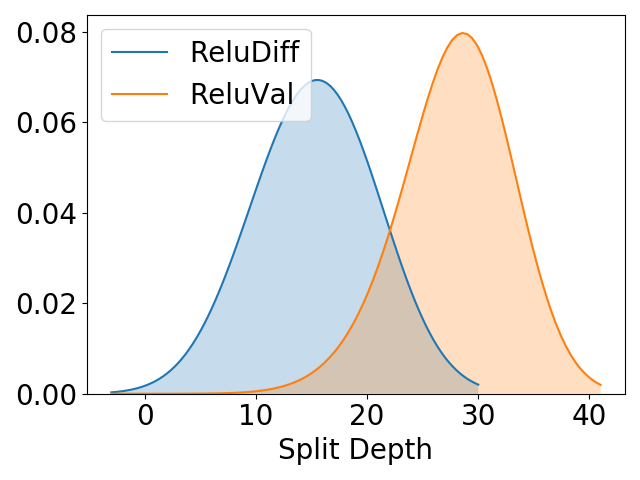
\includegraphics[width=\linewidth]{reludiff/figs/prop4_split_depth.png}
		\caption{$ \phi_4 $ max depth distribution.\label{fig:prop4_depth}}
	\end{minipage}
	\begin{minipage}[t]{0.495\linewidth}
				\captionsetup{width=0.9\textwidth}
			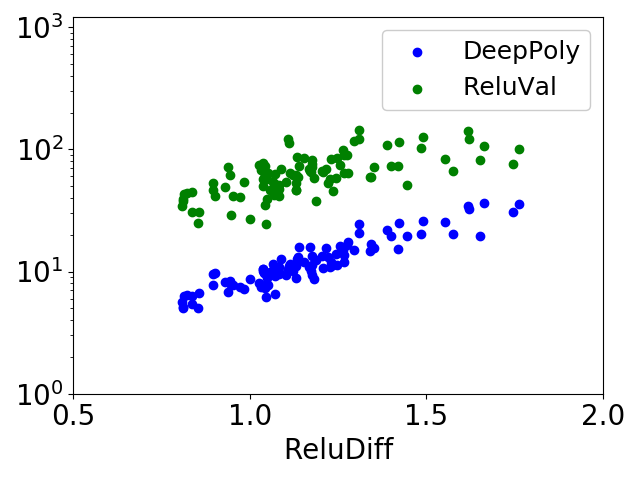
\includegraphics[width=\linewidth]{reludiff/figs/deeppoly_mnist_4_1024_compare.png}
			\caption{$\Delta $-interval on MNIST 4x1024\label{fig:deeppoly_comp}.}
	\end{minipage}%
\end{figure}

\subsubsection{MNIST}

While in ACAS Xu the input region to verify is defined by the
property, for MNIST, we must generate the input region ourselves. We
generate 200 input regions for MNIST using two methods. The first
method is based on global perturbation~\cite{SinghGPV19}. We take 100
test images, and for each one, we allow each of the pixels to be
perturbed by +/-3 gray scale units. The second method is based on
targeted pixel perturbation~\cite{GopinathPWZK19,GopinathKPB18}. We
take the same 100 test images, and for each one, we set the range of 3 random
pixels to $ [0,255] $, while the remaining 781 remain fixed.

\begin{table}
%\caption{Accuracy comparison of \diffNN{}, \ReluVal{} and \DeepPoly{} on MNIST
%networks, where network $f'$ is derived from network $f$ by rounding the weights
%to 3 significant figures, and setting  $\epsilon=2.5$.}
\centering
\caption{Accuracy comparison of the three tools on MNIST.}
\label{tbl:MNIST_accuracy}
\scalebox{1.0}{
\begin{tabular}{|l|c|cc|cc|cc|}\hline
Benchmark & Verif. & \multicolumn{2}{c|}{\diffNN{} (new)}
& \multicolumn{2}{c|}{\ReluVal{}} & \multicolumn{2}{c|}{\DeepPoly} \\
\cline{3-8}
                & problems & proved  & undet. & proved & undet. & proved & undet. \\\hline
\hline

3x100-global     & 100      & 100     &   0    &   47    & 53     & 34    & 66     \\\hline
2x512-global     & 100      & 100     &   0    &   0    & 100     & 0    & 100     \\\hline
4x1024-global    & 100      & 22     &  78    &   0    & 100     & 0   & 100      \\\hline
\hline
3x100-3-pixel     & 100     & 100     &   0    &   100    & 0     & 100    & 0     \\\hline
2x512-3-pixel     & 100     & 100     &   0    &   100    & 0     & 80   & 20     \\\hline
4x1024-3-pixel    & 100     & 100     &  0    &   97    & 3     & 100   & 0      \\\hline


\end{tabular}
}
\end{table}

\begin{table}
%\caption{Efficiency comparison of \diffNN{}, \ReluVal{} and \DeepPoly{} on MNIST
%networks, where network $f'$ is derived from network $f$ by rounding the weights
%to 3 significant figures, and setting  $\epsilon=2.5$.}
\centering
\caption{Efficiency comparison of the three tools on MNIST.}
\label{tbl:MNIST_efficiency}
\scalebox{1.0}{
\begin{tabular}{|l|c|r|r|r|}\hline
Benchmark         & Verif.  & \multicolumn{3}{c|}{ Total Time (s) }\\\cline{3-5}
                  & problems & \diffNN{} (new) & \ReluVal{} & \DeepPoly{} \\\hline
\hline
3x100-global       &     100    &        29.47     &        95458.32          &   118823.09          \\\hline
2x512-global       &     100    &        77.83     &        180000.00          &   180000.0          \\\hline
4x1024-global      &     100    &     141604.53    &        180000.00       &      180000.0     \\\hline
\hline
3x100-3-pixel       &     100   &     23.90    &        32.60            &   163.75         \\\hline
2x512-3-pixel       &     100   &     79.24    &        715.16             &   37674.40         \\\hline
4x1024-3-pixel      &     100   &     296.59       &     92100.10          &    49042.98    \\\hline
\end{tabular}
}
\end{table}


We can again see in Tables~\ref{tbl:MNIST_accuracy}
and \ref{tbl:MNIST_efficiency} that \diffNN{} is significantly more
accurate and efficient than both \ReluVal{} and \DeepPoly{}.
%
Both competing techniques struggle to handle global perturbations even
on the small 3x100 network, let alone the larger 2x512 and 4x1024 networks.
%
On the other hand, \diffNN{} can easily handle both the 3x100 and 2x512 networks,
achieving at least 3 orders of magnitude speedup on these networks.
%
We also see a three orders of magnitude speedup on the two largest networks
for our targeted-pixel perturbation experiments.

Even though \diffNN{} begins to reach its limit in the global perturbation experiment
on the largest 4x1024 network, we point out that \diffNN{} is significantly outperforming
both \DeepPoly{} and \ReluVal{} in the accuracy of their forward passes.
%
Figure~\ref{fig:deeppoly_comp} compares the output bound verified on the
\textit{first, single} forward pass of each technique.
%
The comparison is presented as a scatter plot, where the x-axis is the
bound verified by \diffNN{}, and the y-axis is that of the competing technique.

The graph shows that \diffNN{} is nearly two orders of magnitude more accurate
than \ReluVal{} and one order of magnitude more than \DeepPoly.
%
The improvement over \DeepPoly{} especially emphasizes the promise of \diffNN{}'s
approach. This is because \diffNN{} is already outperforming \DeepPoly{}, yet it
uses a simpler \emph{concretization} approach during the forward pass, whereas
\DeepPoly{} uses a more sophisticated \emph{linear relaxation}.
%
We believe that \diffNN{} can be extended to use more accurate techniques such as
linear relaxation which would further improve the accuracy, however we leave
this as future work.


\subsubsection{HAR}

For HAR, we also created our verification problems using input
perturbation.  We take 100 concrete test inputs, and for each one, we
allow a global perturbation of +/-0.1.
%
The results are summarized in Tables~\ref{tbl:HAR_accuracy} and~\ref{tbl:HAR_efficiency}.
%
%
Again, the experimental comparison shows that \diffNN{} is
significantly more accurate and efficient.



\begin{table}
	\centering
	\caption{Accuracy comparison of the three tools on HAR.}
	\label{tbl:HAR_accuracy}
	\scalebox{1.0}{
		\begin{tabular}{|l|c|cc|cc|cc|}\hline
			Benchmark & Verif. & \multicolumn{2}{c|}{\diffNN{} (new)}
			& \multicolumn{2}{c|}{\ReluVal{}} & \multicolumn{2}{c|}{\DeepPoly} \\
			\cline{3-8}
			& problems & proved  & undet. & proved & undet. & proved & undet. \\\hline
			\hline

			1x500     & 100      & 100     &   0    &   0    &   100   &  0 &  100   \\\hline

		\end{tabular}
	}
\end{table}

\begin{table}
	\centering
	\caption{Efficiency comparison of the three tools on HAR.}
	\label{tbl:HAR_efficiency}
	\scalebox{1.0}{
		\begin{tabular}{|l|c|r|r|r|}\hline
			Benchmark         & Verif.  & \multicolumn{3}{c|}{ Total Time (s) }\\\cline{3-5}
			& problems & \diffNN{} (new) & \ReluVal{} & \DeepPoly{} \\\hline
			\hline
			1x500       &     100    &        28.79     &        180000.00   &   180000.00   \\\hline
		\end{tabular}
	}
\end{table}

\subsection{Threats to Validity}


Our method is designed for verifying neural networks typically found
in control applications, where the number of input signals is not
large. In this context, dividing the input region turns out to be a
very effective way of increasing the accuracy of interval analysis.
However, neural networks in different application domains may have
different characteristics.  Therefore, it remains an open problem
whether bi-section of individual input intervals is always an
effective way of performing refinement.


Our method is designed for feed-forward ReLU networks.  Although there
is no significant technical hurdle for it to be extended to
convolutional neural networks or other activation functions, such as
sigmoid, tanh and max-pool as shown recently by Singh et
al.~\cite{SinghGPV19}, we have not evaluated the effectiveness.
Specifically, linear relaxation can be used to handle these features
when it comes to approximating non-linear behavior.  While we use
concretization in \diffNN{}, extending it with linear relaxation is
possible~\cite{WangPWYJ18nips}. However, we leave these extensions for
future work.


%\section{Related Work}
%\label{sec:related}
%
%While there is a large and growing body of work on detecting
%adversarial examples for neural networks, they are typically based on
%heuristic search or other dynamic analysis techniques such as
%testing~\cite{CarliniW17,PeiCYJ17,TianPJR18,SunWRHKK18,WickerHK18,MaLLZG18}.
%Although they are effective in finding security vulnerabilities and
%violations of other critical properties, we consider them as being
%orthogonal to formal verification.  The reason is because these
%techniques are geared toward finding violations, as opposed to proving
%the absence of violations.
%
%
%Early work on formal verification of deep neural networks relies on
%using SMT solvers~\cite{HuangKWW17,Ehlers17}, or SMT solving
%algorithms~\cite{KatzBDJK17,KatzHIJLLSTWZDK19} designed for
%efficiently reasoning about constraints from the ReLU activation
%function. Along this line, a state-of-the-art tool
%is \Reluplex{}~\cite{KatzBDJK17}.  In theory, these SMT solver based
%techniques can solve the neural network verification problem in a
%sound and complete fashion, i.e., returning a proof if and only if the
%network satisfies the property.  In practice, however, their
%scalability is often limited and they may run out of time for larger
%networks.
%
%
%Another line of work on verification of deep neural networks is based
%on interval analysis, which can be more scalable than
%SMT solver based techniques~\cite{WangPWYJ18}.  They compute
%conservative bounds on the value ranges of the neurons and output
%signals for an input region of interest.  They also exploit the fact
%that neural networks are Lipschitz continuous~\cite{RuanHK18} to
%ensure that the interval analysis results are
%sound.  \ReluVal{}~\cite{WangPWYJ18} and \DeepPoly{}~\cite{SinghGPV19}
%are two representatives, among other similar
%tools~\cite{WangPWYJ18nips,SinghGPV19iclr,MirmanGV18,GehrMDTCV18,FischerBDGZV19}.
%
%
%
%In addition to formal verification, there are techniques for
%evaluating and certifying the robustness of neural
%networks~\cite{BastaniILVNC16,CarliniW17,WengZCSHDBD18,DvijothamSGMK18}
%or certified defense against adversarial
%examples~\cite{RaghunathanSL18,WongK18}.
%%
%However, neither they nor the existing verification techniques
%were designed for \emph{differential verification} of two closely
%related neural networks, which is the focus of this paper.
%%
%%
%As shown by the examples in Section~\ref{sec:motivation} and the
%experimental results in Section~\ref{sec:experiment}, directly
%applying these techniques to differential verification is often
%extremely inefficient.  In contrast, our method is designed
%specifically for solving the differential verification problem efficiently.





At a higher level, our method relies on symbolic interval analysis,
which can be viewed as a specific form of abstract
interpretation~\cite{CousotC77}.  While the abstract interpretation
framework allows approximations to be performed in a more general way,
e.g., using relational abstract domains~\cite{Mine04} such as the
octagon~\cite{Mine01} and polyhedral~\cite{CousotH78} domains, so far,
it has not be adequately explored.  We plan to explore the use of
these abstract domains as part
of the future work.



Finally, the term \textit{differential verification} has been used
in the context of verifying a new version of a program with
respect to a previous version, which is treated as an ``oracle''~\cite{DAC13}.
In a sense, the truncated network is a ``new version'' of the original
network, and the original network can be thought of as an oracle.



\section{Summary}
\label{sec:conclusion}

We have presented a new method, named \diffNN{}, for differential
verification of two closely related neural networks.  It is capable of
formally proving the accuracy of a compressed network with respect to
the original network.  Internally, \diffNN{} relies on symbolic
interval analysis to more accurately compute and propagate differences
in the values of neurons of the two networks from the input to the
output, and then relies on the gradient difference to more accurately
compute the refinement.  Our experimental comparison of \diffNN{} with
state-of-the-art formal verification techniques shows that it can often
achieve two orders of magnitude speedup and produce many more proofs.


\section{Optimization 3 Proofs}
Here we give formal proofs for the un-proven bounds in Section~\ref{sec:opt}.
As in section~\ref{sec:opt}, we rewrite Equations~\ref{eq:1} and~\ref{eq:2} as
\begin{align*}
\deq(n,d) & = \R{n + d} - \R{n}\\
\deq'(n', d) & = \R{n'} - \R{n' - d}.
\end{align*}
where $ n \in \ReluIN{\n}, n' \in \ReluIN{\np}, $ and $ d \in \ReluINdelta{\n} $.

\subsection{Upper Bound of First Case}
Recall this case is $ \LBconcrete{\ReluINdelta{\n}} \geq 0 $.
We derive the bound from Equation~\ref{eq:2} by dividing into two cases, and then combining their result
to get the lower bound.

\subsection*{Case 1: $ n' - d > 0 = n' > d $}
Based on the above constraint, we can simplify $ \deq'(n',d) $ to
\[
	\deq'(n',d) = \R{n'} - (n' - d).
\]
In addition, since we are considering the case where $ \LBconcrete{\ReluINdelta{\n}} \geq 0 $,
we have $ d \geq 0 $. Combining this with our case 1 constraint $ n' > d $,
we have
\[
	n' > d \wedge d \geq 0 \implies n' > 0.
\]
Thus, in case 1, we have that $ \deq'(n',d) $ is just
\[
	\deq'(n',d) = n' - (n' - d) = d.
\]

We also note that $ n' > 0 $ means that
\[
n' > d \iff max(0, n') > d
\]
because $ n' > 0 $ means that $ max(0, n') = n' $. We use this fact when we combine the two cases.

\subsection*{Case 2: $ n' - d \leq 0 = n' \leq d $}
The above constraint allows us to simplify $ \deq'(n',d) $ to
\[
	\deq'(n',d) = \R{n'} - 0 = \R{n'} = max(0, n').
\]
We also note that under our constraints we have
\[
n' \leq d \iff max(0, n') \leq d,
\]
which we will use when we combine the cases. To prove this, first observe that
\[
0 \leq d \wedge n' \leq d \implies max(0, n') \leq d.
\]
That is, if $ d $ is greater-than-or-equal to both 0 and $ n' $, then clearly
it is greater-than-or-equal to the max of the two. And for the other way,
\[
max(0, n') \leq d \implies  n' \leq d.
\]
That is, if $ d $ is greater-than-or-equal to the max of 0 and $ n' $, then clearly
it is greater-than-or-equal to $ n' $.

\subsection*{Combing the Two Cases}
Combining our two cases, we get the function
\[
	\deq'(n',d) = \begin{cases}
	d & n' > d\\
	max(0, n') & n' \leq d
	\end{cases}
\]
and then substituting with the equations we derived at the end of case 1 and 2, we get
\[
\deq'(n',d) = \begin{cases}
d & max(0, n') > d\\
max(0, n') & max(0, n') \leq d
\end{cases} = min(max(0, n'), d)
\]
Since the upper bound of both $ min() $ and $ max() $ occur when we take the upper bounds of their input variables, we get that the upper bound of $ \deq'(n',d) $ is
\begin{align*}
min(max(0, \UBconcrete{\ReluIN{\np}}), \UBconcrete{\ReluINdelta{\n}})\\
= min(\UBconcrete{\ReluIN{\np}}, \UBconcrete{\ReluINdelta{\n}}).
\end{align*}
We can remove the $ max() $ function because $ \np $ is non-linear, so
$ \UBconcrete{\ReluIN{\np}} > 0 $.


\subsection{Lower Bound of Second Case}
Recall this case is $ \UBconcrete{\ReluINdelta{\n}} \leq 0 $. We derive the lower bound from Equation~\ref{eq:1} by dividing into two cases. The proof is symmetric to the previous case.
\subsection*{Case 1: $ n + d > 0 = n > -d = d > -n $}
In this case, we can immediately simplify
\[
	\deq(n,d) = n + d - \R{n}.
\]
Then, since $ \UBconcrete{\ReluINdelta{\n}} \leq 0 $ implies $ d \leq 0 = -d \geq 0 $,
we can use our case 1 constraint $ n > -d $ to derive
\[
	n > -d \wedge -d \geq 0 \implies n > 0.
\]
Thus we can further simplify
\[
	\deq(n,d) = n + d - n = d.
\]

We also note that $ n > 0 = -n < 0 \implies min(0, -n) = -n $, so we also have
\[
	d > -n \iff d > min(0, -n).
\]
We use this fact when combining the two cases.

\subsection*{Case 2: $ n + d \leq 0 = d \leq -n $}
In this case, we can immediately simplify
\[
	\deq(n,d) = 0 - \R{n} = -max(0, n) = min(0, -n).
\]
We also not here that
\[
	d \leq -n \wedge d \leq 0 \iff d \leq min(0, -n).
\]
We use this fact when combining the two cases.

\subsection*{Combining the Cases}
Combing our two cases, we get the function
\[
	\deq(n,d) = \begin{cases}
	d & d > -n\\
	min(0, -n) & d \leq -n
	\end{cases}
\]
and rewriting this equation using the inequalities we derived at the end of case 1 and 2
we get
\[
\deq(n,d) = \begin{cases}
d & d > min(0, -n)\\
min(0, -n) & d \leq min(0, -n)
\end{cases} = max(d, min(0, -n)).
\]
Since the lower bound of both $ min() $ and $ max() $ occur when we minimize their inputs, we get the lower bound of $ \deq(n,d) $ is
\begin{align*}
max(\LBconcrete{\ReluINdelta{\n}}, min(0, -\UBconcrete{\ReluIN{\n}}))\\
= max(\LBconcrete{\ReluINdelta{\n}}, -\UBconcrete{\ReluIN{\n}}).
\end{align*}
We can remove the $ min() $ function because $ \n $ is non-linear so $ -\UBconcrete{\ReluIN{\n}} < 0 $.

\subsection{Lower Bound of Third Case}
Recall this case is $ \LBconcrete{\ReluINdelta{\n}} < 0 < \UBconcrete{\ReluINdelta{\n}} $. We derive the lower bound from Equation~\ref{eq:1}. We divide into two cases and then combine them as done previously.

\subsection*{Case 1: $ n + d > 0 = d > -n $}
$ \deq(n,d) $ simplifies to
\[
	\deq(n,d) = n + d - \R{n}.
\]
We further divide into two sub-cases.

\subsection*{Case 1.1: $ n > 0 $}
$ \deq(n,d) $ further simplifies to
\[
	\deq(n,d) = n + d - n = d.
\]
Since we only care about the lower bound, observe that the lower bound of
case 1.1 occurs when we take the \textit{minimum} value of $ d $, which is \textit{always} less than 0.

\subsection*{Case 1.2: $ n \leq 0 $}
$ \deq(n,d) $ further simplifies to
\[
	\deq(n,d) = n + d - 0 = n + d.
\]
Observe that the lower bound cannot be less than 0 in case 1.2 because of the case 1 constraint.
This means the lower bound \textit{always} occurs in case 1.1, so we can safely ignore case 1.2. (But we emphasize this \textit{only} applies when evaluating $ \deq(n,d) $ for the lower bound).

\subsection*{Case 2: $ n + d \leq 0 = d \leq -n $}
$ \deq(n,d) $ further simplifies to
\[
	\deq(n,d) = 0 - \R{n} = -\R{n}.
\]
We consider the two cases of this function.
\subsection*{Case 2.1: $ n > 0 $}
$ \deq(n,d) $ becomes
\[
	\deq(n,d) = -n.
\]
The minimum value here occurs at the upper bound of $ n $, which is \textit{always} less than 0 because $ \n $ is non-linear.

\subsection*{Case 2.2: $ n \leq 0 $}
$ \deq(n,d) = 0 $ in this case. Since the lower bound of case 2.1 is \textit{always} less than 0, the minimum value will never occur in this case, so we can safely ignore it.


\subsection*{Combining the Cases}
We've shown that the minimum value occurs in either case 1.1 or case 2.1, which gives us the function (however only for the \textit{minimum} value and not the maximum)
\[
\deq(n,d) = \begin{cases}
d & d > -n\\
-n & d \leq -n
\end{cases} = max(-n,d).
\]
Evaluating this function for its lower bounds gives us
\[
 max(-\UBconcrete{\ReluIN{\n}}, \LBconcrete{\ReluINdelta{\n}}).
\]

\subsection{Upper Bound of Third Case}
Recall this case is $ \LBconcrete{\ReluINdelta{\n}} < 0 < \UBconcrete{\ReluINdelta{\n}} $. We derive the upper bound from Equation~\ref{eq:2}. We divide into two cases and then combine them as done previously. This proof mirrors the proof for the lower bound of the third case.

\subsection*{Case 1: $ n' - d > 0 = n' > d $}
$ \deq'(n',d) $ simplifies to
\[
\deq'(n',d) = \R{n'} - n' + d.
\]
We further divide into two sub-cases.

\subsection*{Case 1.1: $ n' > 0 $}
$ \deq'(n',d) $ further simplifies to
\[
\deq'(n',d) = n' - n' + d = d.
\]
Since we only care about the upper bound, observe that the upper bound of
case 1.1 occurs when we take the \textit{maximum} value of $ d $, which is always greater than 0.

\subsection*{Case 1.2: $ n' \leq 0 $}
$ \deq'(n',d) $ further simplifies to
\[
\deq'(n',d) = 0 - n' + d = -n' + d.
\]
Our case 1 constraint $ n' - d > 0 = 0 > -n' + d $ implies the upper bound in case 1.2
can be no greater than 0. This means the upper bound $ \deq'(n',d) $ always occurs in case 1.1, so we
can ignore case 1.2.

\subsection*{Case 2: $ n' - d \leq 0 = n' \leq d $}
$ \deq'(n',d) $ further simplifies to
\[
\deq'(n',d) = \R{n'} - 0 = \R{n'}.
\]
We consider the two cases of this function.
\subsection*{Case 2.1: $ n' > 0 $}
$ \deq'(n',d) $ becomes
\[
	\deq'(n',d) = n',
\]
which has its maximum value at the upper bound of $ n' $.

\subsection*{Case 2.2: $ n' \leq 0 $}
$ \deq(n,d) = 0 $ in this case. Since the upper bound of $ n' $ is greater than 0, the maximum value will never occur in this case, so we can safely ignore it.


\subsection*{Combining the Cases}
We've shown that the maximum value occurs in either case 1.1 or case 2.1, which gives us the function (only for the \textit{maximum} value and not the minimum)
\[
\deq'(n',d) = \begin{cases}
d & n' > d\\
n' & n' \leq d
\end{cases} = min(n',d).
\]
Evaluating this function for its upper bound gives us

\[
	min(\UBconcrete{\ReluIN{\np}}, \UBconcrete{\ReluINdelta{\n}}).
\]





\chapter{Symbolic Approximations for the Difference}
\label{ch:neurodiff}
\declarecommand{\Name}{\textsc{NeuroDiff}}
\declarecommand{\ReluDiffP}{\textsc{ReluDiff+}}
\declarecommand{\ReluDiff}{\textsc{ReluDiff}}

\declarecommand{\ReluVal}{\textsc{ReluVal}}
\declarecommand{\DeepPoly}{\textsc{DeepPoly}}

\declarecommand{\Reluplex}{\textsc{Reluplex}}
\declarecommand{\Neurify}{\textsc{Neurify}}
\declarecommand{\RefineZono}{\textsc{RefineZono}}

\declarecommand{\nj}[0]{n_{k,j}}
\declarecommand{\n}[2]{n_{#1,#2}}
\declarecommand{\np}[2]{n'_{#1,#2}}
\declarecommand{\npj}[0]{n'_{k,j}}
\declarecommand{\nd}[2]{\Delta_{#1,#2}}
\declarecommand{\ndj}{\Delta_{k,j}}
\declarecommand{\W}[3]{W_{#1}[#2,#3]}
\declarecommand{\Wp}[3]{W_{#1}'[#2,#3]}
\declarecommand{\Wk}[1]{W_{#1}}
\declarecommand{\Wd}[3]{W_{#1}^\Delta[#2,#3]}

\declarecommand{\IntIn}[1]{S^{in}(#1)}
\declarecommand{\IntOut}[1]{S(#1)}

\declarecommand{\relu}[1]{ReLU(#1)}

\declarecommand{\UBEq}[1]{\mathsf{UB}(#1)}
\declarecommand{\LBEq}[1]{\mathsf{LB}(#1)}
\declarecommand{\UBU}[1]{\overline{\mathsf{UB}}(#1)}
\declarecommand{\UBL}[1]{\underline{\mathsf{UB}}(#1)}
\declarecommand{\LBL}[1]{\underline{\mathsf{LB}}(#1)}
\declarecommand{\LBU}[1]{\overline{\mathsf{LB}}(#1)}



\theoremstyle{plain}
\newtheorem{thm}{Theorem}
\newtheorem{lemma}{Lemma}

\newtheoremstyle{case}{}{}{}{}{}{:}{ }{}
\theoremstyle{case}
\newtheorem{case}{Case}

%\subsubsection{Need for differential verification}
There is a growing need for rigorous analysis techniques that can
compare the behaviors of two or more neural networks trained for the
same task. For example, such techniques have applications in
better understanding the representations learned by different
networks~\cite{wang2018towards}, and finding inputs where networks
disagree~\cite{xie2019diffchaser}.
%
The need is further motivated by the increasing use of neural network
compression~\cite{HanMD16} -- a technique that alters the network's
parameters to reduce its energy and computational cost -- where
we \textit{expect} the compressed network to be functionally
equivalent to the original network.
%
In safety-critical systems where a single instance of misbehavior can
lead to catastrophe, having \textit{formal guarantees} on the
equivalence of the original and compressed networks is
highly desirable.


%\subsubsection{Limitations of existing methods}
Unfortunately, most work aimed at verifying or testing neural networks
does not provide formal guarantees on their equivalence.  For example,
testing techniques geared toward \emph{refutation} can provide inputs
where a single network misbehaves~\cite{ma2018deepgauge,
xie2019deephunter, SunWRHKK18, TianPJR18, odena2018tensorfuzz} or
multiple networks disagree~\cite{xie2019diffchaser,PeiCYJ17,MaLLZG18},
but they do not guarantee the absence of misbehaviors or disagreements.
%
While techniques geared toward \emph{verification} can prove safety or
robustness properties of a single
network~\cite{HuangKWW17,Ehlers17,KatzHIJLLSTWZDK19,RuanHK18,
WangPWYJ18nips,SinghGPV19iclr,MirmanGV18,GehrMDTCV18,FischerBDGZV19},
they lack crucial information needed to prove the equivalence of
multiple networks.
%
One exception is the \ReluDiff{} tool of Paulsen et
al.~\cite{paulsen2020reludiff}, which computes a sound approximation of the
difference of two neural networks, a problem known as
\textit{differential verification}.  While \ReluDiff{} performs
better than other techniques, the overly conservative approximation it
computes often causes both accuracy and efficiency to suffer.


%\subsubsection{Our main contributions}
To overcome these problems, we propose \Name{}, a new \emph{symbolic}
and \emph{fine-grained} approximation technique that significantly increases the
accuracy of differential verification while achieving many
orders-of-magnitude speedup.
%
\Name{} has two key contributions.  The first contribution is the development
of \emph{convex approximations}, a fine-grained approximation technique
for bounding the output difference of neurons for all possible inputs,
which drastically improves over the
coarse-grained \emph{concretizations} used by \ReluDiff{}.
%
The second contribution is judiciously introducing symbolic variables
to represent neurons in hidden layers whose difference bounds have
accumulated significant approximation error.
%
These two techniques are also complementary, i.e., when combined, the
benefit is significantly greater than the sum of their individual
benefits.



\begin{figure}[t]
	\centering
\scalebox{1.25}{

\tikzset{every picture/.style={line width=0.75pt}} %set default line width to 0.75pt

\begin{tikzpicture}[x=0.75pt,y=0.75pt,yscale=-1,xscale=1]
%uncomment if require: \path (0,300); %set diagram left start at 0, and has height of 300

%Rounded Rect [id:dp4236892252286144]
\draw  [fill={rgb, 255:red, 252; green, 202; blue, 120 }  ,fill opacity=0.5 ] (112,65.85) .. controls (112,62.62) and (114.62,60) .. (117.85,60) -- (164.15,60) .. controls (167.38,60) and (170,62.62) .. (170,65.85) -- (170,171.15) .. controls (170,174.38) and (167.38,177) .. (164.15,177) -- (117.85,177) .. controls (114.62,177) and (112,174.38) .. (112,171.15) -- cycle ;
%Shape: Circle [id:dp7068459723221313]
\draw   (123.61,89.44) .. controls (123.61,85.33) and (126.94,82) .. (131.06,82) .. controls (135.17,82) and (138.5,85.33) .. (138.5,89.44) .. controls (138.5,93.56) and (135.17,96.89) .. (131.06,96.89) .. controls (126.94,96.89) and (123.61,93.56) .. (123.61,89.44) -- cycle ;
%Shape: Circle [id:dp10436586105910262]
\draw   (143.61,89.44) .. controls (143.61,85.33) and (146.94,82) .. (151.06,82) .. controls (155.17,82) and (158.5,85.33) .. (158.5,89.44) .. controls (158.5,93.56) and (155.17,96.89) .. (151.06,96.89) .. controls (146.94,96.89) and (143.61,93.56) .. (143.61,89.44) -- cycle ;
%Shape: Circle [id:dp04586875504356169]
\draw   (113.61,114.56) .. controls (113.61,110.44) and (116.94,107.11) .. (121.06,107.11) .. controls (125.17,107.11) and (128.5,110.44) .. (128.5,114.56) .. controls (128.5,118.67) and (125.17,122) .. (121.06,122) .. controls (116.94,122) and (113.61,118.67) .. (113.61,114.56) -- cycle ;
%Shape: Circle [id:dp23529117657421317]
\draw   (133.61,114.56) .. controls (133.61,110.44) and (136.94,107.11) .. (141.06,107.11) .. controls (145.17,107.11) and (148.5,110.44) .. (148.5,114.56) .. controls (148.5,118.67) and (145.17,122) .. (141.06,122) .. controls (136.94,122) and (133.61,118.67) .. (133.61,114.56) -- cycle ;
%Shape: Circle [id:dp18975621582850755]
\draw   (153.61,114.56) .. controls (153.61,110.44) and (156.94,107.11) .. (161.06,107.11) .. controls (165.17,107.11) and (168.5,110.44) .. (168.5,114.56) .. controls (168.5,118.67) and (165.17,122) .. (161.06,122) .. controls (156.94,122) and (153.61,118.67) .. (153.61,114.56) -- cycle ;
%Straight Lines [id:da39358625060202257]
\draw    (131.06,96.89) -- (121.06,107.11) ;
%Straight Lines [id:da7050149301027024]
\draw    (131.06,96.89) -- (141.06,107.11) ;
%Straight Lines [id:da078846190833607]
\draw    (131.06,96.89) -- (161.06,107.11) ;
%Straight Lines [id:da2611151157782621]
\draw    (151.06,96.89) -- (161.06,107.11) ;
%Straight Lines [id:da854791249594143]
\draw    (151.06,96.89) -- (141.06,107.11) ;
%Straight Lines [id:da003907601781767633]
\draw    (151.06,96.89) -- (121.06,107.11) ;
%Shape: Circle [id:dp5156337693032028]
\draw   (158.5,164.56) .. controls (158.5,168.67) and (155.17,172) .. (151.06,172) .. controls (146.94,172) and (143.61,168.67) .. (143.61,164.56) .. controls (143.61,160.44) and (146.94,157.11) .. (151.06,157.11) .. controls (155.17,157.11) and (158.5,160.44) .. (158.5,164.56) -- cycle ;
%Shape: Circle [id:dp06607101355690326]
\draw   (138.5,164.56) .. controls (138.5,168.67) and (135.17,172) .. (131.06,172) .. controls (126.94,172) and (123.61,168.67) .. (123.61,164.56) .. controls (123.61,160.44) and (126.94,157.11) .. (131.06,157.11) .. controls (135.17,157.11) and (138.5,160.44) .. (138.5,164.56) -- cycle ;
%Shape: Circle [id:dp10601416223357618]
\draw   (168.5,139.44) .. controls (168.5,143.56) and (165.17,146.89) .. (161.06,146.89) .. controls (156.94,146.89) and (153.61,143.56) .. (153.61,139.44) .. controls (153.61,135.33) and (156.94,132) .. (161.06,132) .. controls (165.17,132) and (168.5,135.33) .. (168.5,139.44) -- cycle ;
%Shape: Circle [id:dp25720293065397004]
\draw   (148.5,139.44) .. controls (148.5,143.56) and (145.17,146.89) .. (141.06,146.89) .. controls (136.94,146.89) and (133.61,143.56) .. (133.61,139.44) .. controls (133.61,135.33) and (136.94,132) .. (141.06,132) .. controls (145.17,132) and (148.5,135.33) .. (148.5,139.44) -- cycle ;
%Shape: Circle [id:dp4093542080553124]
\draw   (128.5,139.44) .. controls (128.5,143.56) and (125.17,146.89) .. (121.06,146.89) .. controls (116.94,146.89) and (113.61,143.56) .. (113.61,139.44) .. controls (113.61,135.33) and (116.94,132) .. (121.06,132) .. controls (125.17,132) and (128.5,135.33) .. (128.5,139.44) -- cycle ;
%Straight Lines [id:da8322313642706787]
\draw    (151.06,157.11) -- (161.06,146.89) ;
%Straight Lines [id:da4076421006538775]
\draw    (151.06,157.11) -- (141.06,146.89) ;
%Straight Lines [id:da22036650281611347]
\draw    (151.06,157.11) -- (121.06,146.89) ;
%Straight Lines [id:da5955438584611725]
\draw    (131.06,157.11) -- (121.06,146.89) ;
%Straight Lines [id:da6153976114126399]
\draw    (131.06,157.11) -- (141.06,146.89) ;
%Straight Lines [id:da9953813996835473]
\draw    (131.06,157.11) -- (161.06,146.89) ;

%Straight Lines [id:da23986906826746157]
\draw    (121.06,122) -- (141.06,132) ;
%Straight Lines [id:da2936393327105673]
\draw    (121.06,122) -- (161.06,132) ;
%Straight Lines [id:da5774592223000948]
\draw    (141.06,122) -- (121.06,132) ;
%Straight Lines [id:da027247136169882613]
\draw    (141.06,122) -- (141.06,132) ;
%Straight Lines [id:da2078286476738037]
\draw    (141.06,122) -- (161.06,132) ;
%Straight Lines [id:da07067307391973043]
\draw    (161.06,122) -- (161.06,132) ;
%Straight Lines [id:da5480660909270823]
\draw    (161.06,122) -- (141.06,132) ;
%Straight Lines [id:da6293253437621619]
\draw    (161.06,122) -- (121.06,132) ;
%Straight Lines [id:da7407175241217754]
\draw    (121.06,122) -- (121.06,132) ;

%Rounded Rect [id:dp2355420157466821]
\draw  [fill={rgb, 255:red, 252; green, 202; blue, 120 }  ,fill opacity=0.5 ] (50,182.02) .. controls (50,180.9) and (50.9,180) .. (52.02,180) -- (105.98,180) .. controls (107.1,180) and (108,180.9) .. (108,182.02) -- (108,197.98) .. controls (108,199.1) and (107.1,200) .. (105.98,200) -- (52.02,200) .. controls (50.9,200) and (50,199.1) .. (50,197.98) -- cycle ;
%Rounded Rect [id:dp39333818742980176]
\draw  [fill={rgb, 255:red, 144; green, 195; blue, 255 }  ,fill opacity=0.5 ] (180,74.13) .. controls (180,66.33) and (186.33,60) .. (194.13,60) -- (355.87,60) .. controls (363.67,60) and (370,66.33) .. (370,74.13) -- (370,185.87) .. controls (370,193.67) and (363.67,200) .. (355.87,200) -- (194.13,200) .. controls (186.33,200) and (180,193.67) .. (180,185.87) -- cycle ;
%Rounded Rect [id:dp15859389295109172]
\draw   (246,70.5) .. controls (253.73,70.5) and (260,76.77) .. (260,84.5) -- (260,176) .. controls (260,183.73) and (253.73,190) .. (246,190) -- (204,190) .. controls (196.27,190) and (190,183.73) .. (190,176) -- (190,84.5) .. controls (190,76.77) and (196.27,70.5) .. (204,70.5) -- cycle ;
%Straight Lines [id:da09167228503135971]
\draw    (170,100) -- (187,100) ;
\draw [shift={(190,100)}, rotate = 180] [fill={rgb, 255:red, 0; green, 0; blue, 0 }  ][line width=0.08]  [draw opacity=0] (8.93,-4.29) -- (0,0) -- (8.93,4.29) -- cycle    ;
%Straight Lines [id:da15082942023264767]
\draw    (170,190) -- (189.35,102.93) ;
\draw [shift={(190,100)}, rotate = 462.53] [fill={rgb, 255:red, 0; green, 0; blue, 0 }  ][line width=0.08]  [draw opacity=0] (8.93,-4.29) -- (0,0) -- (8.93,4.29) -- cycle    ;
%Rounded Rect [id:dp19836331083326175]
\draw  [fill={rgb, 255:red, 252; green, 202; blue, 120 }  ,fill opacity=0.5 ] (112,182.02) .. controls (112,180.9) and (112.9,180) .. (114.02,180) -- (167.98,180) .. controls (169.1,180) and (170,180.9) .. (170,182.02) -- (170,197.98) .. controls (170,199.1) and (169.1,200) .. (167.98,200) -- (114.02,200) .. controls (112.9,200) and (112,199.1) .. (112,197.98) -- cycle ;
%Rounded Rect [id:dp3414447171885684]
\draw   (190,163.86) .. controls (190,156.2) and (196.2,150) .. (203.86,150) -- (246.14,150) .. controls (253.8,150) and (260,156.2) .. (260,163.86) -- (260,176.14) .. controls (260,183.8) and (253.8,190) .. (246.14,190) -- (203.86,190) .. controls (196.2,190) and (190,183.8) .. (190,176.14) -- cycle ;
%Rounded Rect [id:dp7331605414728447]
\draw   (190,123.36) .. controls (190,115.7) and (196.2,109.5) .. (203.86,109.5) -- (246.14,109.5) .. controls (253.8,109.5) and (260,115.7) .. (260,123.36) -- (260,135.64) .. controls (260,143.3) and (253.8,149.5) .. (246.14,149.5) -- (203.86,149.5) .. controls (196.2,149.5) and (190,143.3) .. (190,135.64) -- cycle ;
%Rounded Rect [id:dp724286819012004]
\draw   (356,170) .. controls (358.21,170) and (360,171.79) .. (360,174) -- (360,186) .. controls (360,188.21) and (358.21,190) .. (356,190) -- (294,190) .. controls (291.79,190) and (290,188.21) .. (290,186) -- (290,174) .. controls (290,171.79) and (291.79,170) .. (294,170) -- cycle ;
%Rounded Rect [id:dp8526981920637079]
\draw   (355.84,125) .. controls (358.14,125) and (360,126.86) .. (360,129.16) -- (360,141.62) .. controls (360,143.92) and (358.14,145.78) .. (355.84,145.78) -- (294.16,145.78) .. controls (291.86,145.78) and (290,143.92) .. (290,141.62) -- (290,129.16) .. controls (290,126.86) and (291.86,125) .. (294.16,125) -- cycle ;
%Rounded Rect [id:dp6803009958438129]
\draw   (354,70) .. controls (357.31,70) and (360,72.69) .. (360,76) -- (360,94) .. controls (360,97.31) and (357.31,100) .. (354,100) -- (296,100) .. controls (292.69,100) and (290,97.31) .. (290,94) -- (290,76) .. controls (290,72.69) and (292.69,70) .. (296,70) -- cycle ;
%Straight Lines [id:da323377208231176]
\draw    (300,170) -- (300,149) ;
\draw [shift={(300,146)}, rotate = 450] [fill={rgb, 255:red, 0; green, 0; blue, 0 }  ][line width=0.08]  [draw opacity=0] (8.93,-4.29) -- (0,0) -- (8.93,4.29) -- cycle    ;
%Straight Lines [id:da9479303756560082]
\draw    (301,125) -- (301,103) ;
\draw [shift={(301,100)}, rotate = 450] [fill={rgb, 255:red, 0; green, 0; blue, 0 }  ][line width=0.08]  [draw opacity=0] (8.93,-4.29) -- (0,0) -- (8.93,4.29) -- cycle    ;
%Straight Lines [id:da32236695764284484]
\draw    (260,180) -- (287,180) ;
\draw [shift={(290,180)}, rotate = 180] [fill={rgb, 255:red, 0; green, 0; blue, 0 }  ][line width=0.08]  [draw opacity=0] (8.93,-4.29) -- (0,0) -- (8.93,4.29) -- cycle    ;
%Straight Lines [id:da551116351892766]
\draw    (360,135) -- (397,135) ;
\draw [shift={(400,135)}, rotate = 180] [fill={rgb, 255:red, 0; green, 0; blue, 0 }  ][line width=0.08]  [draw opacity=0] (8.93,-4.29) -- (0,0) -- (8.93,4.29) -- cycle    ;
%Rounded Rect [id:dp9869780674255966]
\draw  [fill={rgb, 255:red, 252; green, 202; blue, 120 }  ,fill opacity=0.5 ] (50,65.85) .. controls (50,62.62) and (52.62,60) .. (55.85,60) -- (102.15,60) .. controls (105.38,60) and (108,62.62) .. (108,65.85) -- (108,171.15) .. controls (108,174.38) and (105.38,177) .. (102.15,177) -- (55.85,177) .. controls (52.62,177) and (50,174.38) .. (50,171.15) -- cycle ;
%Shape: Circle [id:dp8539692235458093]
\draw   (61.61,89.44) .. controls (61.61,85.33) and (64.94,82) .. (69.06,82) .. controls (73.17,82) and (76.5,85.33) .. (76.5,89.44) .. controls (76.5,93.56) and (73.17,96.89) .. (69.06,96.89) .. controls (64.94,96.89) and (61.61,93.56) .. (61.61,89.44) -- cycle ;
%Shape: Circle [id:dp1487342990764624]
\draw   (81.61,89.44) .. controls (81.61,85.33) and (84.94,82) .. (89.06,82) .. controls (93.17,82) and (96.5,85.33) .. (96.5,89.44) .. controls (96.5,93.56) and (93.17,96.89) .. (89.06,96.89) .. controls (84.94,96.89) and (81.61,93.56) .. (81.61,89.44) -- cycle ;
%Shape: Circle [id:dp35573619874650775]
\draw   (51.61,114.56) .. controls (51.61,110.44) and (54.94,107.11) .. (59.06,107.11) .. controls (63.17,107.11) and (66.5,110.44) .. (66.5,114.56) .. controls (66.5,118.67) and (63.17,122) .. (59.06,122) .. controls (54.94,122) and (51.61,118.67) .. (51.61,114.56) -- cycle ;
%Shape: Circle [id:dp43998418948198004]
\draw   (71.61,114.56) .. controls (71.61,110.44) and (74.94,107.11) .. (79.06,107.11) .. controls (83.17,107.11) and (86.5,110.44) .. (86.5,114.56) .. controls (86.5,118.67) and (83.17,122) .. (79.06,122) .. controls (74.94,122) and (71.61,118.67) .. (71.61,114.56) -- cycle ;
%Shape: Circle [id:dp11364870191253851]
\draw   (91.61,114.56) .. controls (91.61,110.44) and (94.94,107.11) .. (99.06,107.11) .. controls (103.17,107.11) and (106.5,110.44) .. (106.5,114.56) .. controls (106.5,118.67) and (103.17,122) .. (99.06,122) .. controls (94.94,122) and (91.61,118.67) .. (91.61,114.56) -- cycle ;
%Straight Lines [id:da5311768222051036]
\draw    (69.06,96.89) -- (59.06,107.11) ;
%Straight Lines [id:da8245862905976873]
\draw    (69.06,96.89) -- (79.06,107.11) ;
%Straight Lines [id:da9037048113348528]
\draw    (69.06,96.89) -- (99.06,107.11) ;
%Straight Lines [id:da6775367181725077]
\draw    (89.06,96.89) -- (99.06,107.11) ;
%Straight Lines [id:da20764974600729147]
\draw    (89.06,96.89) -- (79.06,107.11) ;
%Straight Lines [id:da4787036285423938]
\draw    (89.06,96.89) -- (59.06,107.11) ;
%Shape: Circle [id:dp6787178527201608]
\draw   (96.5,164.56) .. controls (96.5,168.67) and (93.17,172) .. (89.06,172) .. controls (84.94,172) and (81.61,168.67) .. (81.61,164.56) .. controls (81.61,160.44) and (84.94,157.11) .. (89.06,157.11) .. controls (93.17,157.11) and (96.5,160.44) .. (96.5,164.56) -- cycle ;
%Shape: Circle [id:dp8189142658483558]
\draw   (76.5,164.56) .. controls (76.5,168.67) and (73.17,172) .. (69.06,172) .. controls (64.94,172) and (61.61,168.67) .. (61.61,164.56) .. controls (61.61,160.44) and (64.94,157.11) .. (69.06,157.11) .. controls (73.17,157.11) and (76.5,160.44) .. (76.5,164.56) -- cycle ;
%Shape: Circle [id:dp21275076334366427]
\draw   (106.5,139.44) .. controls (106.5,143.56) and (103.17,146.89) .. (99.06,146.89) .. controls (94.94,146.89) and (91.61,143.56) .. (91.61,139.44) .. controls (91.61,135.33) and (94.94,132) .. (99.06,132) .. controls (103.17,132) and (106.5,135.33) .. (106.5,139.44) -- cycle ;
%Shape: Circle [id:dp1824568474340943]
\draw   (86.5,139.44) .. controls (86.5,143.56) and (83.17,146.89) .. (79.06,146.89) .. controls (74.94,146.89) and (71.61,143.56) .. (71.61,139.44) .. controls (71.61,135.33) and (74.94,132) .. (79.06,132) .. controls (83.17,132) and (86.5,135.33) .. (86.5,139.44) -- cycle ;
%Shape: Circle [id:dp825767248504503]
\draw   (66.5,139.44) .. controls (66.5,143.56) and (63.17,146.89) .. (59.06,146.89) .. controls (54.94,146.89) and (51.61,143.56) .. (51.61,139.44) .. controls (51.61,135.33) and (54.94,132) .. (59.06,132) .. controls (63.17,132) and (66.5,135.33) .. (66.5,139.44) -- cycle ;
%Straight Lines [id:da6766885451674735]
\draw    (89.06,157.11) -- (99.06,146.89) ;
%Straight Lines [id:da08122409377631135]
\draw    (89.06,157.11) -- (79.06,146.89) ;
%Straight Lines [id:da8441374241505181]
\draw    (89.06,157.11) -- (59.06,146.89) ;
%Straight Lines [id:da7442737845395763]
\draw    (69.06,157.11) -- (59.06,146.89) ;
%Straight Lines [id:da9566636567575862]
\draw    (69.06,157.11) -- (79.06,146.89) ;
%Straight Lines [id:da19409192754236826]
\draw    (69.06,157.11) -- (99.06,146.89) ;

%Straight Lines [id:da39227385116907143]
\draw    (59.06,122) -- (79.06,132) ;
%Straight Lines [id:da16288130182449367]
\draw    (59.06,122) -- (99.06,132) ;
%Straight Lines [id:da19810001689574364]
\draw    (79.06,122) -- (59.06,132) ;
%Straight Lines [id:da24191813694330322]
\draw    (79.06,122) -- (79.06,132) ;
%Straight Lines [id:da1525732415062876]
\draw    (79.06,122) -- (99.06,132) ;
%Straight Lines [id:da22405676573237499]
\draw    (99.06,122) -- (99.06,132) ;
%Straight Lines [id:da9334192766546668]
\draw    (99.06,122) -- (79.06,132) ;
%Straight Lines [id:da3285219924463475]
\draw    (99.06,122) -- (59.06,132) ;
%Straight Lines [id:da28988712234136327]
\draw    (59.06,122) -- (59.06,132) ;

%Straight Lines [id:da08693151331707771]
\draw    (290,80) -- (263,80) ;
\draw [shift={(260,80)}, rotate = 360] [fill={rgb, 255:red, 0; green, 0; blue, 0 }  ][line width=0.08]  [draw opacity=0] (8.93,-4.29) -- (0,0) -- (8.93,4.29) -- cycle    ;
%Straight Lines [id:da3246311983059058]
\draw    (290,90) -- (263,90) ;
\draw [shift={(260,90)}, rotate = 360] [fill={rgb, 255:red, 0; green, 0; blue, 0 }  ][line width=0.08]  [draw opacity=0] (8.93,-4.29) -- (0,0) -- (8.93,4.29) -- cycle    ;

% Text Node
\draw (53,47) node [anchor=north west][inner sep=0.75pt]   [align=left] {\small
Inputs};
% Text Node
\draw (184,48) node [anchor=north west][inner sep=0.75pt]   [align=left] {\small
NeuroDiff};
% Text Node
\draw (196,76.5) node [anchor=north west][inner sep=0.75pt]   [align=left] {\begin{minipage}[lt]{40.70935600000001pt}\setlength\topsep{0pt}
	\begin{center}
	{\small Forward}\\{\small Analysis}
	\end{center}

	\end{minipage}};
% Text Node
\draw (183,114.5) node [anchor=north west][inner sep=0.75pt]   [align=left] {\begin{minipage}[lt]{61.370000000000005pt}\setlength\topsep{0pt}
	\begin{center}
	{\scriptsize Convex}\\{\scriptsize Approximation}
	\end{center}

	\end{minipage}};
% Text Node
\draw (187.5,157) node [anchor=north west][inner sep=0.75pt]   [align=left] {\begin{minipage}[lt]{53.720000000000006pt}\setlength\topsep{0pt}
	\begin{center}
	{\scriptsize Intermediate}\\{\scriptsize Variables}
	\end{center}

	\end{minipage}};
% Text Node
\draw (296,173.5) node [anchor=north west][inner sep=0.75pt]   [align=left] {\begin{minipage}[lt]{39.848000000000006pt}\setlength\topsep{0pt}
	\begin{center}
	Check $\displaystyle \epsilon $
	\end{center}

	\end{minipage}};
% Text Node
\draw (369,125) node [anchor=north west][inner sep=0.75pt]  [font=\footnotesize] [align=left] {\begin{minipage}[lt]{16.025356000000002pt}\setlength\topsep{0pt}
	\begin{center}
	Yes
	\end{center}

	\end{minipage}};
% Text Node
\draw (397,129) node [anchor=north west][inner sep=0.75pt]  [font=\footnotesize] [align=left] {\begin{minipage}[lt]{29.931356pt}\setlength\topsep{0pt}
	\begin{center}
	Verified
	\end{center}

	\end{minipage}};
% Text Node
\draw (296.5,72) node [anchor=north west][inner sep=0.75pt]   [align=left] {\begin{minipage}[lt]{40.154pt}\setlength\topsep{0pt}
	\begin{center}
	{\footnotesize Partition $\displaystyle X$}
	\end{center}

	\end{minipage}};
% Text Node
\draw (307,111) node [anchor=north west][inner sep=0.75pt]  [font=\footnotesize] [align=left] {\begin{minipage}[lt]{13.146644000000002pt}\setlength\topsep{0pt}
	\begin{center}
	No
	\end{center}

	\end{minipage}};
% Text Node
\draw (57.56,65.5) node [anchor=north west][inner sep=0.75pt]   [align=left] {\begin{minipage}[lt]{30.498000000000005pt}\setlength\topsep{0pt}
	\begin{center}
	$ f $
	\end{center}

	\end{minipage}};
% Text Node
\draw (119.56,65.5) node [anchor=north west][inner sep=0.75pt]   [align=left] {\begin{minipage}[lt]{30.498000000000005pt}\setlength\topsep{0pt}
	\begin{center}
	$ f' $
	\end{center}

	\end{minipage}};
% Text Node
\draw (113.06,183.5) node [anchor=north west][inner sep=0.75pt]   [align=left] {\begin{minipage}[lt]{40.63pt}\setlength\topsep{0pt}
	\begin{center}
	$\displaystyle X\subseteq \mathbb{R}^{n}$
	\end{center}

	\end{minipage}};
% Text Node
\draw (73.56,186.5) node [anchor=north west][inner sep=0.75pt]   [align=left] {\begin{minipage}[lt]{8.67pt}\setlength\topsep{0pt}
	\begin{center}
	$\displaystyle \epsilon $
	\end{center}

	\end{minipage}};
% Text Node
\draw (269,67) node [anchor=north west][inner sep=0.75pt]   [align=left] {\begin{minipage}[lt]{16.127356000000002pt}\setlength\topsep{0pt}
	\begin{center}
	$\displaystyle X_{1}$
	\end{center}

	\end{minipage}};
% Text Node
\draw (269,92) node [anchor=north west][inner sep=0.75pt]   [align=left] {\begin{minipage}[lt]{16.127356000000002pt}\setlength\topsep{0pt}
	\begin{center}
	$\displaystyle X_{2}$
	\end{center}

	\end{minipage}};
% Text Node
\draw (296.5,128.83) node [anchor=north west][inner sep=0.75pt]   [align=left] {\begin{minipage}[lt]{40.732pt}\setlength\topsep{0pt}
	\begin{center}
	Proven?
	\end{center}

	\end{minipage}};


\end{tikzpicture}
}
\caption{The overall flow of \Name{}.}
\label{neurodiff:fig:diagram}
\end{figure}


%\subsubsection{Overall flow of our method}
The overall flow of \Name{} is shown in Figure~\ref{neurodiff:fig:diagram},
where it takes as input two neural networks $ f $ and $ f' $, a set of
inputs to the neural networks $ X $ defined by box intervals, and a small
constant $ \epsilon $ that quantifies the tolerance for disagreement. We assume
that $ f $ and $ f' $ have the same network topology and only differ in the
numerical values of their weights. In practice, $ f' $ could be the compressed
version of $ f $, or they could be networks constructed using the same network
topology but slightly different training data. We also note that this
assumption can support compression techniques such as weight
pruning~\cite{HanMD16} (by setting edges' weights to 0) and even neuron
removal~\cite{gokulanathan2019simplifying} (by setting all of a neuron's
incoming edge weights to 0). \Name{} then aims to prove $
\forall
x \in X. |f'(x) - f(x)| < \epsilon $. It can return
(1) \emph{verified} if a proof can be found, or
(2) \emph{undetermined} if a specified timeout is reached.


Internally, \Name{} first performs a forward analysis using symbolic
interval arithmetic to bound both the absolute value ranges of all
neurons, as in single network verification, and the difference between
the neurons of the two networks. \Name{} then checks if the difference
between the output neurons satisfies $ \epsilon $, and if so
returns \emph{verified}. Otherwise,
\Name{} uses a gradient-based refinement to partition $ X
$ into two disjoint sub regions $ X_1 $ and $ X_2 $, and attempts the
analysis again on the individual regions. Since $ X_1 $ and $ X_2 $
form independent sub-problems, we can do these analyses in parallel,
hence gaining significant speedup.
%  (a) interval arithmetic to propagate absolute value ranges
%  (b) interval arithmetic to propagate difference value ranges
%  (c) multi-threading to perform forward interval analysis
%  (d) gradient based refinement to partition input regions


%\subsubsection{Convex approximation: what's new?}
The new convex approximations used in \Name{} are significantly more
accurate than not only the coarse-grained \emph{concretizations}
in \ReluDiff{}~\cite{paulsen2020reludiff} but also the standard convex
approximations in single-network verification tools~\cite{SinghGPV19,
Singh2019krelu, WangPWYJ18nips, zhang2018efficient}.
%
While these (standard) convex approximations aim to bound the absolute
value range of $ y = \relu{x} $, where $x$ is the input of
the \textit{rectified linear unit} (ReLU) activation function, our new
convex approximations aim to bound the difference $ z = \relu{x
+ \Delta} - \relu{x} $, where $x$ and $x+\Delta$ are ReLU inputs of
two corresponding neurons.
%
This is significantly more challenging because it involves the search
of bounding planes in a three-dimensional space (defined by $x$,
$\Delta$ and $z$) as opposed to a two-dimensional space as in the
prior work.


%\subsubsection{Symbolic variables: what's new?}
The symbolic variables we judiciously add to represent values of
neurons in hidden layers should not be confused with the symbolic
inputs used by existing tools either.
%
While the use of symbolic inputs is well understood, e.g., both in
single-network verification~\cite{SinghGPV19, Singh2019krelu,
WangPWYJ18nips, zhang2018efficient} and differential
verification~\cite{paulsen2020reludiff}, this is the first time that symbolic
variables are used to substitute values of hidden neurons during
differential verification.
%
While the impact of symbolic inputs often diminishes after the first
few layers of neurons, the impact of these new symbolic variables,
when judiciously added, can be maintained in any hidden layer.


%\subsubsection{Experiments: does it work?}
We have implemented the proposed \Name{} in a tool and evaluated it on
a large set of differential verification tasks. Our benchmarks
consists of 49 networks, from applications such as aircraft collision
avoidance, image classification, and human activity recognition.  We
have experimentally compared with \ReluDiff{}~\cite{paulsen2020reludiff}, the
state-of-the-art tool which has also been shown to be superior to
\ReluVal{}~\cite{WangPWYJ18} and \DeepPoly{}~\cite{SinghGPV19} for differential
verification.
%
Our results show that \Name{} is up to 1,000X faster and 5X more
accurate.  In addition, \Name{} is able to prove many of the same properties
as \ReluDiff{} while considering much larger input regions.


To summarize, this paper makes the following contributions:
\begin{itemize}
\item
We propose new convex approximations to more accurately bound the
difference between corresponding neurons of two structurally similar
neural networks.
\item
We propose a method for judiciously introducing symbolic variables to
neurons in hidden layers to mitigate the propagation of approximation
error.
\item
We implement and evaluate the proposed technique on a large number of
differential verification tasks and demonstrate its significant speed
and accuracy gains.
\end{itemize}


The remainder of this chapter is organized as follows.  First, we
provide a brief overview of our method in Section~\ref{neurodiff:sec:overview}.
Then, we provide the technical background in
Section~\ref{neurodiff:sec:preliminary}.  Next, we present the detailed
algorithms in Section~\ref{neurodiff:sec:approach} and the experimental results
in Section~\ref{neurodiff:sec:experiment}. Finally, we summarize the contributions
of this chapter in Section~\ref{neurodiff:sec:conclusion}.



\section{Overview}
\label{neurodiff:sec:overview}

In this section, we highlight our main contributions and illustrate
the shortcomings of previous work on a motivating example.


\begin{figure}
	\centering
\scalebox{1.25}{

\tikzset{every picture/.style={line width=0.75pt}} %set default line width to 0.75pt

\begin{tikzpicture}[x=0.75pt,y=0.75pt,yscale=-1,xscale=1]
%uncomment if require: \path (0,395); %set diagram left start at 0, and has height of 395

%Shape: Circle [id:dp29452950296941915]
%\draw   (90,55) .. controls (90,41.19) and (101.19,30) .. (115,30) .. controls (128.81,30) and (140,41.19) .. (140,55) .. controls (140,68.81) and (128.81,80) .. (115,80) .. controls (101.19,80) and (90,68.81) .. (90,55) -- cycle ;
\draw (115,55) +(-25,-20) rectangle +(25,20) ;
%Shape: Circle [id:dp7730288688046164]
%\draw   (90,160) .. controls (90,146.19) and (101.19,135) .. (115,135) .. controls (128.81,135) and (140,146.19) .. (140,160) .. controls (140,173.81) and (128.81,185) .. (115,185) .. controls (101.19,185) and (90,173.81) .. (90,160) -- cycle ;
\draw (115,160) +(-25,-20) rectangle +(25,20) ;
%Shape: Circle [id:dp7848793538270885]
\draw   (190,160) .. controls (190,146.19) and (201.19,135) .. (215,135) .. controls (228.81,135) and (240,146.19) .. (240,160) .. controls (240,173.81) and (228.81,185) .. (215,185) .. controls (201.19,185) and (190,173.81) .. (190,160) -- cycle ;
%Shape: Circle [id:dp2581761932666119]
\draw   (190,55) .. controls (190,41.19) and (201.19,30) .. (215,30) .. controls (228.81,30) and (240,41.19) .. (240,55) .. controls (240,68.81) and (228.81,80) .. (215,80) .. controls (201.19,80) and (190,68.81) .. (190,55) -- cycle ;
%Shape: Circle [id:dp03162623697960232]
\draw   (290,160) .. controls (290,146.19) and (301.19,135) .. (315,135) .. controls (328.81,135) and (340,146.19) .. (340,160) .. controls (340,173.81) and (328.81,185) .. (315,185) .. controls (301.19,185) and (290,173.81) .. (290,160) -- cycle ;
%Shape: Circle [id:dp02546394024001375]
\draw   (290,55) .. controls (290,41.19) and (301.19,30) .. (315,30) .. controls (328.81,30) and (340,41.19) .. (340,55) .. controls (340,68.81) and (328.81,80) .. (315,80) .. controls (301.19,80) and (290,68.81) .. (290,55) -- cycle ;
%Shape: Circle [id:dp12084775666404268]
%\draw   (371,105) .. controls (371,91.19) and (382.19,80) .. (396,80) .. controls (409.81,80) and (421,91.19) .. (421,105) .. controls (421,118.81) and (409.81,130) .. (396,130) .. controls (382.19,130) and (371,118.81) .. (371,105) -- cycle ;
\draw (396,105) +(-25,-20) rectangle +(25,20) ;
%Straight Lines [id:da34998381745971496]
\draw    (140,160) -- (187,160) ;
\draw [shift={(190,160)}, rotate = 180] [fill={rgb, 255:red, 0; green, 0; blue, 0 }  ][line width=0.08]  [draw opacity=0] (10.72,-5.15) -- (0,0) -- (10.72,5.15) -- (7.12,0) -- cycle    ;
%Straight Lines [id:da4638805061238097]
\draw    (140,160) -- (188.71,57.71) ;
\draw [shift={(190,55)}, rotate = 475.46] [fill={rgb, 255:red, 0; green, 0; blue, 0 }  ][line width=0.08]  [draw opacity=0] (10.72,-5.15) -- (0,0) -- (10.72,5.15) -- (7.12,0) -- cycle    ;
%Straight Lines [id:da15742477491714235]
\draw    (140,55) -- (187,55) ;
\draw [shift={(190,55)}, rotate = 180] [fill={rgb, 255:red, 0; green, 0; blue, 0 }  ][line width=0.08]  [draw opacity=0] (10.72,-5.15) -- (0,0) -- (10.72,5.15) -- (7.12,0) -- cycle    ;
%Straight Lines [id:da9054930639679811]
\draw    (140,55) -- (188.71,157.29) ;
\draw [shift={(190,160)}, rotate = 244.54000000000002] [fill={rgb, 255:red, 0; green, 0; blue, 0 }  ][line width=0.08]  [draw opacity=0] (10.72,-5.15) -- (0,0) -- (10.72,5.15) -- (7.12,0) -- cycle    ;
%Straight Lines [id:da0727882271401632]
\draw    (240,160) -- (288.71,57.71) ;
\draw [shift={(290,55)}, rotate = 475.46] [fill={rgb, 255:red, 0; green, 0; blue, 0 }  ][line width=0.08]  [draw opacity=0] (10.72,-5.15) -- (0,0) -- (10.72,5.15) -- (7.12,0) -- cycle    ;
%Straight Lines [id:da02068180741540726]
\draw    (240,55) -- (288.71,157.29) ;
\draw [shift={(290,160)}, rotate = 244.54000000000002] [fill={rgb, 255:red, 0; green, 0; blue, 0 }  ][line width=0.08]  [draw opacity=0] (10.72,-5.15) -- (0,0) -- (10.72,5.15) -- (7.12,0) -- cycle    ;
%Straight Lines [id:da4941096166166473]
\draw    (340,55) -- (369.42,102.45) ;
\draw [shift={(371,105)}, rotate = 238.2] [fill={rgb, 255:red, 0; green, 0; blue, 0 }  ][line width=0.08]  [draw opacity=0] (10.72,-5.15) -- (0,0) -- (10.72,5.15) -- (7.12,0) -- cycle    ;
%Straight Lines [id:da0005753242144755921]
\draw    (340,160) -- (369.53,107.61) ;
\draw [shift={(371,105)}, rotate = 479.41] [fill={rgb, 255:red, 0; green, 0; blue, 0 }  ][line width=0.08]  [draw opacity=0] (10.72,-5.15) -- (0,0) -- (10.72,5.15) -- (7.12,0) -- cycle    ;
%Straight Lines [id:da6663993224468625]
\draw    (240,160) -- (287,160) ;
\draw [shift={(290,160)}, rotate = 180] [fill={rgb, 255:red, 0; green, 0; blue, 0 }  ][line width=0.08]  [draw opacity=0] (10.72,-5.15) -- (0,0) -- (10.72,5.15) -- (7.12,0) -- cycle    ;
%Straight Lines [id:da971612493075633]
\draw    (240,55) -- (287,55) ;
\draw [shift={(290,55)}, rotate = 180] [fill={rgb, 255:red, 0; green, 0; blue, 0 }  ][line width=0.08]  [draw opacity=0] (10.72,-5.15) -- (0,0) -- (10.72,5.15) -- (7.12,0) -- cycle    ;

% Text Node
\draw (165,43) node  [font=\normalsize] [align=left] {1.9};
% Text Node
\draw (140,90) node  [font=\normalsize] [align=left] {1.1};
% Text Node
\draw (140,120) node  [font=\normalsize] [align=left] {\mbox{-}1.9};
% Text Node
\draw (165,172.5) node  [font=\normalsize] [align=left] {1.0};
% Text Node
\draw (265,42.5) node  [font=\normalsize] [align=left] {2.1};
% Text Node
\draw (238,90) node  [font=\normalsize] [align=left] {0.9};
% Text Node
\draw (265,172.5) node  [font=\normalsize] [align=left] {1.1};
% Text Node
\draw (238,120) node  [font=\normalsize] [align=left] {\mbox{-}1.0};
% Text Node
\draw (366.5,69) node  [font=\normalsize] [align=left] {1.0};
% Text Node
\draw (369,141) node  [font=\normalsize] [align=left] {\mbox{-}1.0};
% Text Node
\draw (115,55) node  {$n_{0,1}$};
% Text Node
\draw (115,160) node    {$n_{0,2}$};
% Text Node
\draw (215,160) node    {$n_{1,2}$};
% Text Node
\draw (215,55) node    {$n_{1,1}$};
% Text Node
\draw (315,55) node    {$n_{2,1}$};
% Text Node
\draw (315,160) node    {$n_{2,2}$};
% Text Node
\draw (396,105) node    {$n_{3,1}$};
% Text Node
\draw (52,57) node    {$x_{1} \in [ -2,2]$};
% Text Node
\draw (52,161) node    {$x_{2} \in [ -2,2]$};
% Text Node
\draw (118.5,120) node  [font=\normalsize,color={rgb, 255:red, 74; green, 144; blue, 226 }  ,opacity=1 ] [align=left] {\mbox{-}2.0};
% Text Node
\draw (119.5,90) node  [font=\normalsize,color={rgb, 255:red, 74; green, 144; blue, 226 }  ,opacity=1 ] [align=left] {1.0};
% Text Node
\draw (165,29.5) node  [font=\normalsize,color={rgb, 255:red, 74; green, 144; blue, 226 }  ,opacity=1 ] [align=left] {2.0};
% Text Node
\draw (165,185.5) node  [font=\normalsize,color={rgb, 255:red, 74; green, 144; blue, 226 }  ,opacity=1 ] [align=left] {1.0};
% Text Node
\draw (213.5,120) node  [font=\normalsize,color={rgb, 255:red, 74; green, 144; blue, 226 }  ,opacity=1 ] [align=left] {\mbox{-}1.0};
% Text Node
\draw (213.5,90) node  [font=\normalsize,color={rgb, 255:red, 74; green, 144; blue, 226 }  ,opacity=1 ] [align=left] {1.0};
% Text Node
\draw (265,29.5) node  [font=\normalsize,color={rgb, 255:red, 74; green, 144; blue, 226 }  ,opacity=1 ] [align=left] {2.0};
% Text Node
\draw (265,185.5) node  [font=\normalsize,color={rgb, 255:red, 74; green, 144; blue, 226 }  ,opacity=1 ] [align=left] {1.0};
% Text Node
\draw (366.5,56.5) node  [font=\normalsize,color={rgb, 255:red, 74; green, 144; blue, 226 }  ,opacity=1 ] [align=left] {1.0};
% Text Node
\draw (369,154.5) node  [font=\normalsize,color={rgb, 255:red, 74; green, 144; blue, 226 }  ,opacity=1 ] [align=left] {\mbox{-}1.0};


\end{tikzpicture}
}
\caption{Motivating example.}
\label{neurodiff:fig:motex}
\end{figure}



\subsection{Differential Verification}

We use the neural network in Figure~\ref{neurodiff:fig:motex} as a running
example. The network has two input nodes $ \n{0}{1}, \n{0}{2} $, two
hidden layers with two neurons each ($ \n{1}{1}, \n{1}{2} $ and
$ \n{2}{1}, \n{2}{2}$), and one output node $ \n{3}{1} $.  Each neuron
in the hidden layer performs a summation of their inputs, followed by
a \textit{rectified linear unit} (ReLU) activation function, defined
as $ y = max(0,x) $, where $ x $ is the input to the ReLU activation
function, and $ y $ is the output.

Let this entire network be $ f $, and the value of the output node be
$ \n{3}{1} = f(x_1, x_2) $, where $ x_1$ and $x_2 $ are the values of
input nodes $ \n{0}{1}$ and $\n{0}{2} $, respectively.
%
The network can be evaluated on a specific input by performing a
series matrix multiplications (i.e., affine transformations) followed
by element-wise ReLU transformations. For example, the output of
the neurons of the first hidden layer is
\[
\begin{bmatrix}
\n{1}{1} \\
\n{1}{2}
\end{bmatrix}
=
ReLU\Bigg(
\begin{bmatrix}
1.9 & -1.9 \\
1.0 & 1.1
\end{bmatrix}
\cdot
\begin{bmatrix}
x_1 \\
x_2
\end{bmatrix}
\Bigg)
=
\begin{bmatrix}
ReLU(1.9x_1 - 1.9x_2) \\
ReLU(1.1x_1 + 1.0x_2)
\end{bmatrix}
\]

Differential verification aims to compare $ f $ to another network $
f' $ that is structurally similar. For our example, $f'$ is
obtained by rounding the edge weights of $ f $ to the nearest whole
numbers, a network compression technique known as \textit{weight
quantization}.
%
Thus, $ f' $, $ \np{k}{j} $ and $ \np{3}{1} = f'(x_1, x_2) $ are
counterparts of $ f $, $ \n{k}{j} $ and $ \n{3}{1} = f(x_1, x_2) $ for
$0\leq k\leq 2$ and $1\leq j\leq 2$.
%
Our goal is to prove that $ |f'(x_1, x_2) - f(x_1, x_2)| $ is less
than some reasonably small $ \epsilon $ for all inputs defined by the
intervals $ x_1 \in [-2,2]$ and $x_2 \in [-2,2] $.
%
For ease of understanding, we show the edge weights of $ f $ in black, and
$ f' $ in light blue in Figure~\ref{neurodiff:fig:motex}.


\subsection{Limitations of Existing Methods}

Naively, one could adapt any state-of-the-art, single-network
verification tool for our task,
including \DeepPoly{}~\cite{SinghGPV19}
and \Neurify{}~\cite{WangPWYJ18nips}.
%
\Neurify{}, in particular, takes a neural network and
an input region of the network, and uses interval
arithmetic~\cite{moore2009introduction, WangPWYJ18} to produce sound
symbolic lower and upper bounds for each output node.
Typically, \Neurify{} would then use the computed bounds to certify
the absence of \textit{adversarial
examples}~\cite{szegedy2013intriguing} for the network.

However, for our task, the bounds must be computed for both networks $
f $ and $ f' $.  Then, we subtract them, and concretize to compute
lower and upper bounds on $ f'(x_1, x_2) - f(x_1, x_2) $.
%
In our example, the individual bounds would be (approximately, due to
rounding) $[LB(f),UB(f)] = [-0.94x_1 -0.62x_2 -6.51, $ $ 0.71x_1
-2.35x_2 +7.98] $ and $ [LB(f'),UB(f')] = [-0.94x_1 -0.44x_2 -6.75,$ $
0.75x_1 -2.25x_2 +8.00] $ for nodes $ \n{3}{1} $ and $ \np{3}{1} $,
respectively.  After the subtraction, we would obtain the bounds
$[LB(f')-UB(f), UB(f')-LB(f)] = $ $ [-1.65x_1 + 1.9x_2 - 14.73,
1.68x_1 - 1.63x_2 + 14.5] $.  After concretization, we would obtain
the bounds $ [-21.83, 21.12] $.  Unfortunately, the bounds are far
from being accurate.

The \ReluDiff{} method of Paulsen et al.~\cite{paulsen2020reludiff} showed
that, by directly computing a \textit{difference interval}
layer-by-layer, the accuracy can be greatly improved.  For the running
example, \ReluDiff{} would first compute bounds on the difference
between the neurons $ \n{1}{1} $ and $ \np{1}{1} $, which is $ [0,
1.1] $, and then similarly compute bounds on the difference between
outputs of $ \n{1}{2} $ and $ \np{1}{2} $. Then, the results would be
used to compute difference bounds of the subsequent layer.
%
The reason it is more accurate is because it begins computing part of
the difference bound \emph{before} errors have accumulated, whereas
the naive approach first accumulates significant errors at each
neuron, and \emph{then} computes the difference bound.
%
In our running example, \ReluDiff{}~\cite{paulsen2020reludiff} would
compute the tighter bounds $ [-3.1101, 2.5600] $.


While \ReluDiff{} improves over the naive approach, in many cases,
it uses \emph{concrete} values for the upper and lower bounds.
In practice, this approach can suffer from severe error-explosion.
Specifically,
whenever a neuron of either network is in an \textit{unstable} state --
i.e., when a ReLU's input interval contains the value 0 -- it has to
concretize the symbolic expressions.



\subsection{Our Method}


\begin{figure*}
\centering
%
\begin{minipage}[t]{0.45\linewidth}
\centering
%\captionsetup{width=0.98\textwidth}
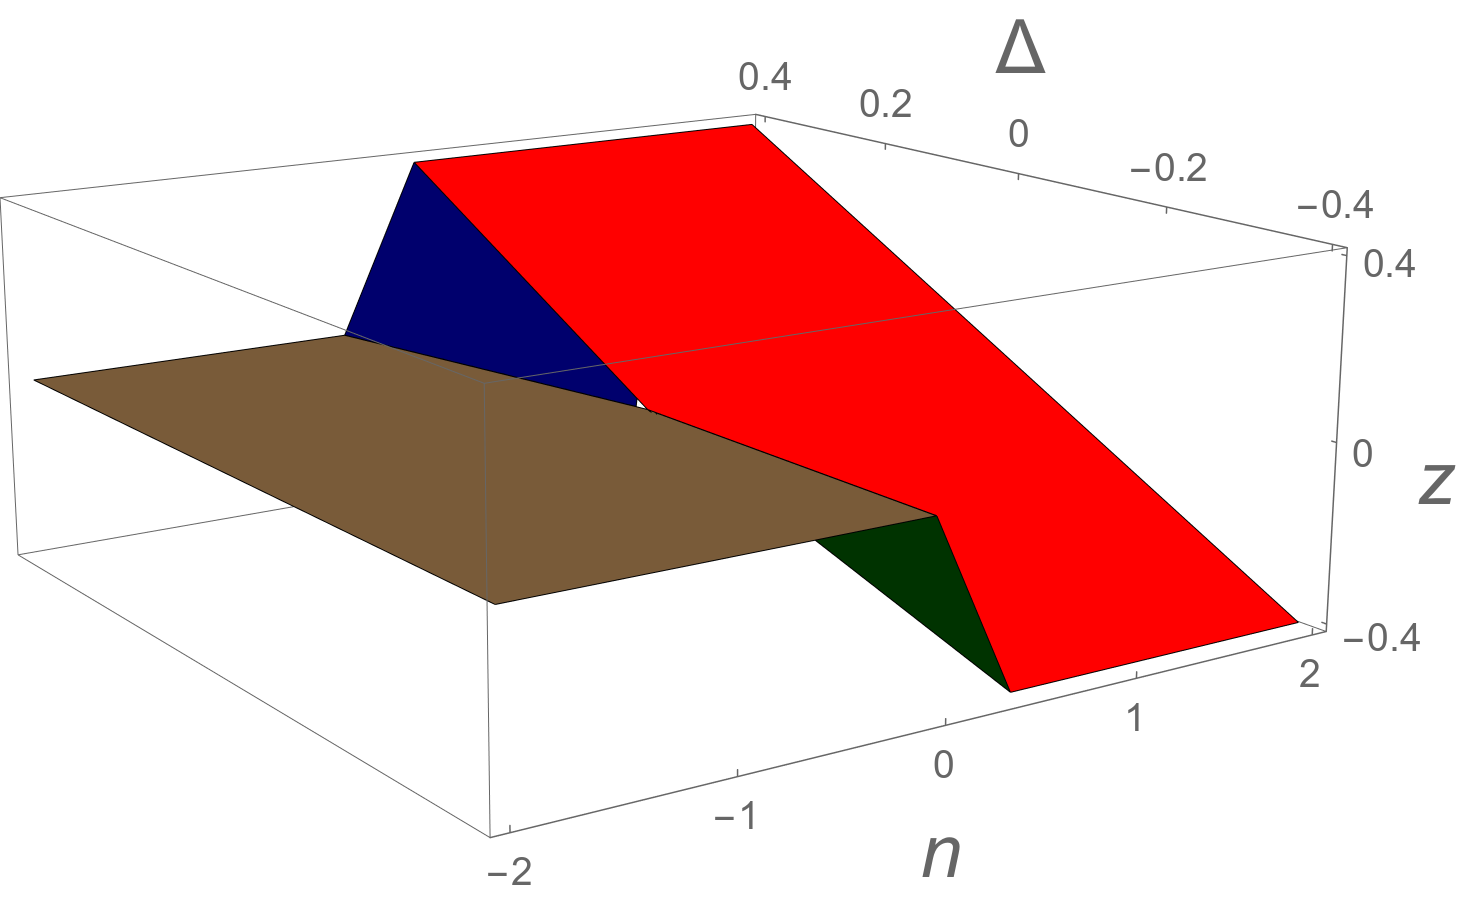
\includegraphics[width=\linewidth]{neurodiff/figs/equation1.png}
\caption{The shape of $ z = ReLU(n + \Delta) - ReLU(n) $.}
\label{neurodiff:fig:equation1}
\end{minipage}%
%
\hspace{0.09\linewidth}
%
\begin{minipage}[t]{0.45\linewidth}
\centering
%\captionsetup{width=0.98\textwidth}
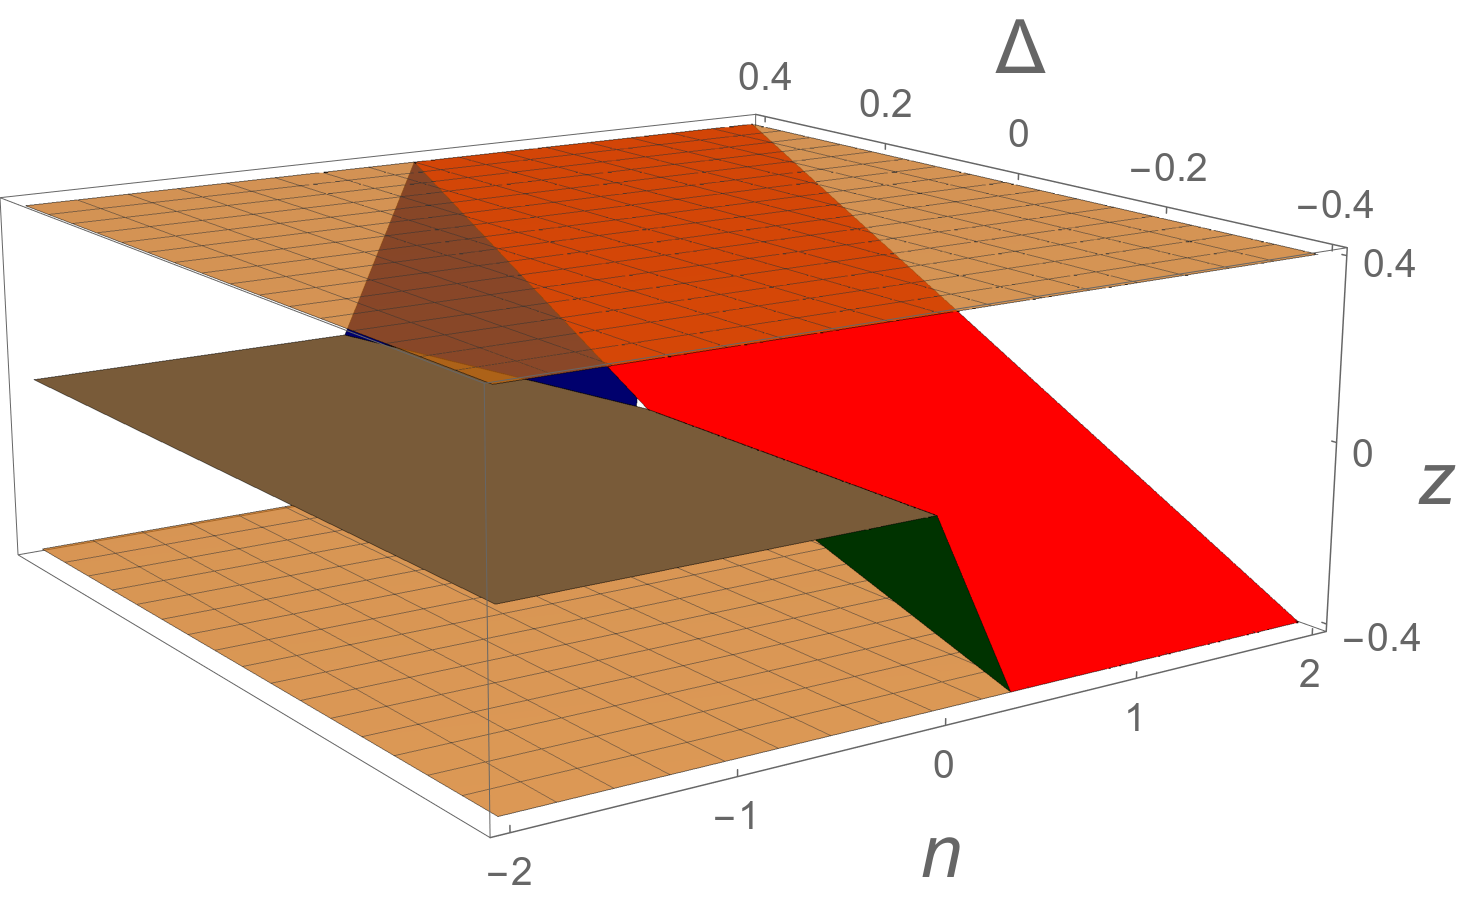
\includegraphics[width=\linewidth]{neurodiff/figs/naiveboundingplanes.png}
\caption{Bounding planes computed by \ReluDiff{}~\cite{paulsen2020reludiff}.}
\label{neurodiff:fig:naiveboundingplanes}
\end{minipage}

\begin{minipage}[t]{0.45\linewidth}
\centering
%\captionsetup{width=0.98\textwidth}
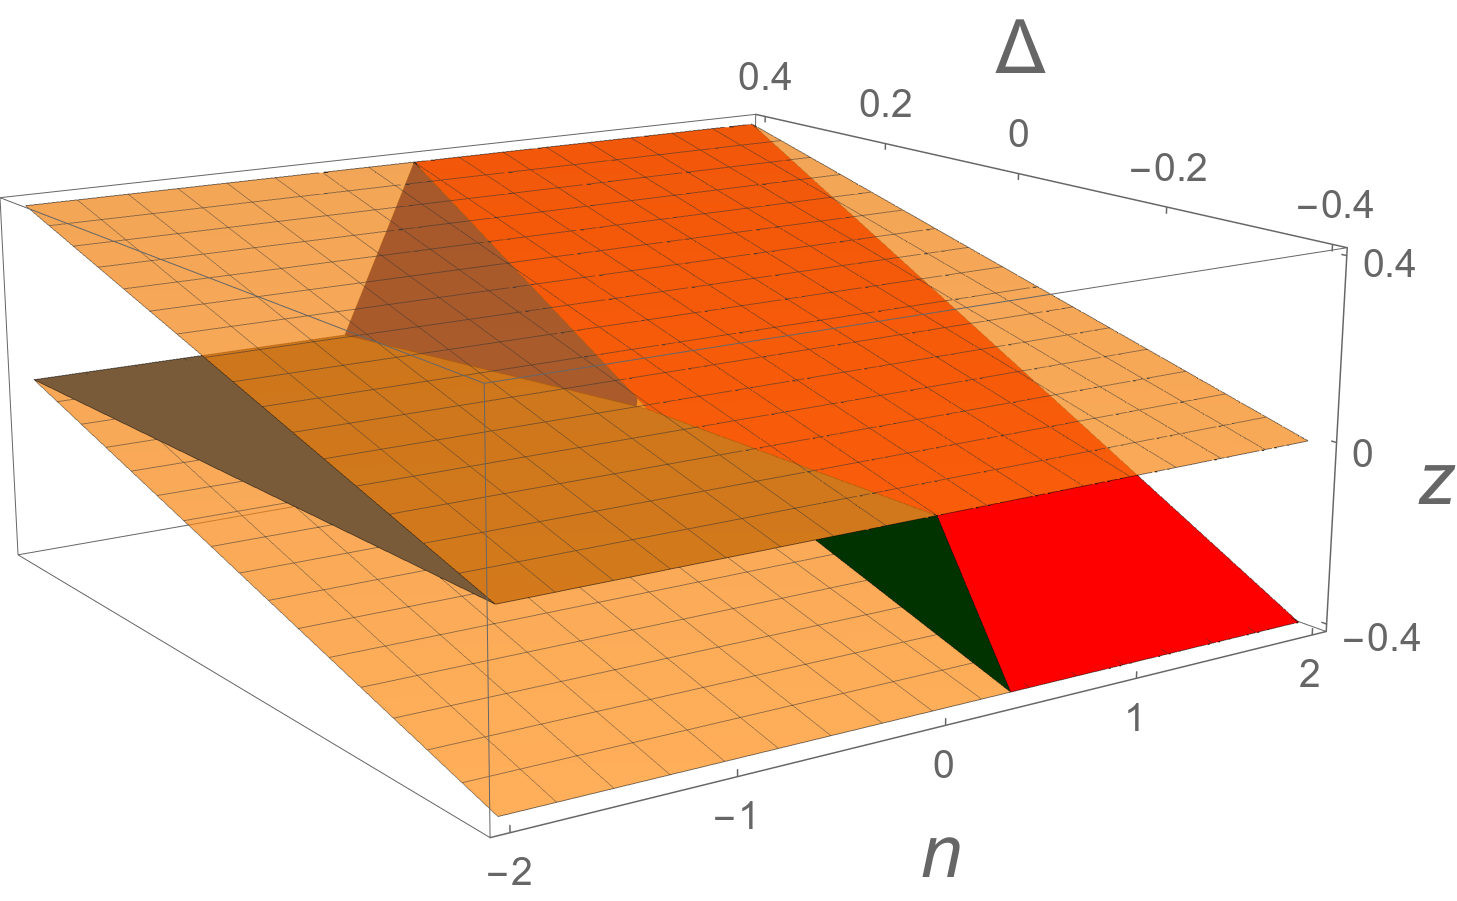
\includegraphics[width=\linewidth]{neurodiff/figs/linearboundingplanes.png}
\caption{Bounding planes computed by our new method.}
\label{neurodiff:fig:linearboundingplanes}
\end{minipage}%
%
\hspace{0.09\linewidth}
%
\begin{minipage}[t]{0.45\linewidth}
\centering
\scalebox{.65}{

\tikzset{every picture/.style={line width=0.75pt}} %set default line width to 0.75pt        

\begin{tikzpicture}[x=0.75pt,y=0.75pt,yscale=-1,xscale=1]
%uncomment if require: \path (0,300); %set diagram left start at 0, and has height of 300

%Straight Lines [id:da5621186100506654] 
\draw [color={rgb, 255:red, 199; green, 199; blue, 199 }  ,draw opacity=1 ]   (102,180) -- (338,180) ;
\draw [shift={(340,180)}, rotate = 180] [color={rgb, 255:red, 199; green, 199; blue, 199 }  ,draw opacity=1 ][line width=0.75]    (10.93,-3.29) .. controls (6.95,-1.4) and (3.31,-0.3) .. (0,0) .. controls (3.31,0.3) and (6.95,1.4) .. (10.93,3.29)   ;
\draw [shift={(100,180)}, rotate = 0] [color={rgb, 255:red, 199; green, 199; blue, 199 }  ,draw opacity=1 ][line width=0.75]    (10.93,-3.29) .. controls (6.95,-1.4) and (3.31,-0.3) .. (0,0) .. controls (3.31,0.3) and (6.95,1.4) .. (10.93,3.29)   ;
%Straight Lines [id:da9708804498380784] 
\draw [color={rgb, 255:red, 199; green, 199; blue, 199 }  ,draw opacity=1 ]   (220,62) -- (220,238) ;
\draw [shift={(220,240)}, rotate = 270] [color={rgb, 255:red, 199; green, 199; blue, 199 }  ,draw opacity=1 ][line width=0.75]    (10.93,-3.29) .. controls (6.95,-1.4) and (3.31,-0.3) .. (0,0) .. controls (3.31,0.3) and (6.95,1.4) .. (10.93,3.29)   ;
\draw [shift={(220,60)}, rotate = 90] [color={rgb, 255:red, 199; green, 199; blue, 199 }  ,draw opacity=1 ][line width=0.75]    (10.93,-3.29) .. controls (6.95,-1.4) and (3.31,-0.3) .. (0,0) .. controls (3.31,0.3) and (6.95,1.4) .. (10.93,3.29)   ;
%Straight Lines [id:da43894388755903013] 
\draw [color={rgb, 255:red, 74; green, 144; blue, 226 }  ,draw opacity=1 ][line width=1.5]    (220,180) -- (340,60) ;
%Straight Lines [id:da1261778605228432] 
\draw [color={rgb, 255:red, 74; green, 144; blue, 226 }  ,draw opacity=1 ][line width=1.5]    (220,180) -- (100,180) ;
%Straight Lines [id:da002818047409691604] 
\draw [color={rgb, 255:red, 0; green, 0; blue, 0 }  ,draw opacity=1 ] [dash pattern={on 4.5pt off 4.5pt}]  (320,80) -- (120,180) ;
%Straight Lines [id:da1715235527986837] 
\draw [color={rgb, 255:red, 0; green, 0; blue, 0 }  ,draw opacity=1 ] [dash pattern={on 4.5pt off 4.5pt}]  (320,130) -- (120,230) ;
%Straight Lines [id:da21391376020902975] 
\draw    (120,175.28) -- (120,180) ;
%Straight Lines [id:da9349071337756625] 
\draw    (120,180) -- (120,184.72) ;
%Straight Lines [id:da2699517570437805] 
\draw    (320,175.28) -- (320,180) ;
%Straight Lines [id:da4265291468096436] 
\draw    (320,180) -- (320,184.72) ;

% Text Node
\draw (117.5,196) node  [font=\Large]  {$\underline{LB}\left( n \right)$};
% Text Node
\draw (337,196) node  [font=\Large]  {$\overline{UB}\left( n \right)$};
% Text Node
\draw (166.5,140.5) node  [font=\Large,rotate=-333.19]  {$UB( ReLU(n) )$};
% Text Node
\draw (300,152.46) node  [font=\Large,rotate=-333.19]  {$LB( ReLU(n) )$};


\end{tikzpicture}
}
\caption{Bounding planes computed by \Neurify{}~\cite{WangPWYJ18nips}.}
\label{neurodiff:fig:wangconvex}
\end{minipage}
\end{figure*}


The key contribution in \Name{}, our new method, is a \emph{symbolic}
and \emph{fine-grained} approximation technique that both reduces the
approximation error introduced when a neuron is in an unstable state,
and mitigates the explosion of such approximation error after it is
introduced.


\subsubsection{Convex Approximation for the Difference Interval}

Our first contribution is developing convex approximations to directly
bound the difference between two neurons after these ReLU activations.
Specifically, for a neuron $ n $ in $ f $ and corresponding neuron $
n' $ in $ f' $, we want to bound the value of $ \relu{n'} - \relu{n}
$. We illustrate the various choices using
Figures~\ref{neurodiff:fig:equation1}, \ref{neurodiff:fig:naiveboundingplanes},
and~\ref{neurodiff:fig:linearboundingplanes}.


The naive way to bound this difference is to first compute
approximations of $ y = \relu{n} $ and $ y' = \relu{n'} $ separately,
and then subtract them.  Since each of these functions has a single
variable, convex approximation is simple and is already used by
single-network verification tools~\cite{SinghGPV19,WangPWYJ18nips,WengZCSHDBD18}.
Figure~\ref{neurodiff:fig:wangconvex} shows the function $y=\relu{n}$ and its
bounding planes (shown as dashed-lines) in a two-dimensional space (details in
Section~\ref{neurodiff:sec:preliminary}).
%
However, as we have already mentioned, approximation errors would be
accumulated in the bounds of $\relu{n}$ and $\relu{n'}$ and then amplified
by the interval subtraction.  This is precisely why the naive approach
performs poorly.


The \ReluDiff{} method of Paulsen et al.~\cite{paulsen2020reludiff} improves
upon the new approximation by computing an interval bound on $ n' - n
$, denoted $ \Delta $, then rewriting $z = \relu{n'} - \relu{n} $ as $
z= \relu{n + \Delta} - \relu{n} $, and finally bounding this new
function instead.
%
Figure~\ref{neurodiff:fig:equation1} shows the shape of $ z = \relu{n
+ \Delta}- \relu{n} $ in a three-dimensional space. Note that it has
four piece-wise linear subregions, defined by values of the input
variables $n$ and $\Delta$.
%
While the bounds computed by \ReluDiff{}~\cite{paulsen2020reludiff}, shown as
the (horizontal) yellow planes in
Figure~\ref{neurodiff:fig:naiveboundingplanes}, are sound, in practice they tend
to be loose because the upper and lower bounds are both concrete
values.  Such eager concretization eliminates symbolic information
that $ \Delta $ contained before applying the ReLU activation.


In contrast, our method computes a convex approximation of $ z $,
shown by the (tilted) yellow planes in
Figure~\ref{neurodiff:fig:linearboundingplanes}.
%
Since these tilted bounding planes are in a three-dimensional space,
they are significantly more challenging to compute than the standard
two-dimensional convex approximations (shown in
Figure~\ref{neurodiff:fig:wangconvex})
used by single network verification tools.
%convex approximation (shown in Figure~\ref{neurodiff:fig:wangconvex}) in a
%two-dimentionsl space, which was used by single-network verification
%tools.
%
Our approximations have the advantage of introducing significantly less
error than the horizontal planes used
in \ReluDiff{}~\cite{paulsen2020reludiff}, while maintaining some of the
symbolic information for $ \Delta $ before applying the ReLU
activation.


We will show through experimental evaluation
(Section~\ref{neurodiff:sec:experiment}) that our convex approximation can
drastically improve the accuracy of the difference bounds, and are
particularly effective when the input region being considered is
large.  Furthermore, the tilted planes shown in
Figure~\ref{neurodiff:fig:linearboundingplanes} are for the general case.  For
certain special cases, we obtain even tighter bounding planes (details
in Section~\ref{neurodiff:sec:approach}).
%
In the running example, using our new convex approximations would
improve the final bounds to $ [-1.97, 1.42] $.


\subsubsection{Symbolic Variables for Hidden Neurons}

Our second contribution is introducing symbolic variables to represent
the output values of some unstable neurons, with the goal of limiting
the propagation of approximation errors after they are introduced.
%
In the running example, since both $ \n{1}{1} $ and $ \np{1}{1} $ are in unstable states,
i.e., the input intervals of the ReLUs contain the value 0, we may introduce a
new
symbol $ x_3 = \relu{\np{1}{1}} - \relu{\n{1}{1}} $.  In all
subsequent layers, whenever the value of $\relu{\np{1}{1}}
- \relu{\n{1}{1}}$ is needed, we use the bounds $[x_3,x_3]$ instead of
the actual bounds.


The reason why using $x_3$ can lead to more accurate results is
because, even though our convex approximations reduce the error
introduced, there is inevitably some error that accumulates. Introducing $
x_3 $ allows this error to partially cancel in the subsequent
layers. In our running example, introducing the new symbolic variable
$x_3$ would be able to improve the final bounds to $ [-1.65, 1.18] $.


While creating $ x_3 $ improved the result
in this case, carelessly introducing new variables for all the unstable
neurons can actually reduce the overall benefit (see
Section~\ref{neurodiff:sec:approach}). In addition, the
computational cost of introducing new variables is not negligible.
%While substituting the values of unstable neurons with new symoblic
%variables may increases the accuracy of interval analysis, it may also
%add computational cost.
Therefore, in practice, we must introduce
these symbolic variables judiciously, to maximize the benefit.
%
Part of our contribution in \Name{} is in developing heuristics to
automatically determine when to create new symbolic variables (details
in Section~\ref{neurodiff:sec:approach}).



\section{Background}
\label{neurodiff:sec:preliminary}

In this section, we review the technical background and then introduce
notations that we use throughout the paper.

\subsection{Neural Networks}

% Define a neural network
% Limit ourselves to FFN ReLU networks
% Weight matrix notation
%	- W_k is the matrix for layer k
%	- W_k[i,j] is the weight of connection from n_k-1,i to n_k,j
We focus on feed-forward neural networks, which we define as a function $ f $ that takes
an $ n $-dimensional vector of real values $x \in \mathbb{X}$, where
$\mathbb{X} \subseteq \mathbb{R}^n $, and maps it to an $ m
$-dimensional vector $ y \in \mathbb{Y}$, where
$\mathbb{Y} \subseteq \mathbb{R}^m $.  We denote this function as $ f
: \mathbb{X} \to \mathbb{Y} $.  Typically, each dimension of $ y $
represents a score, such as a probability, that the input $ x $
belongs to class $ i $, where $ 1 \leq i \leq m $.

A network with $l$ layers has $ l $ weight matrices, each of which is
denoted $ \Wk{k}, $ for $ 1 \leq k \leq l $. For each weight matrix, we
have $ \Wk{k} \in \mathbb{R}^{l_{k-1} \times l_k} $ where $ l_{k-1} $
is the number of neurons in layer $ (k-1) $ and likewise for $ l_k $,
and $ l_0 = n $.
Each element in $ \Wk{k} $ represents the weight of an edge from a
neuron in layer $ (k-1) $ to one in layer $ k $. Let $ \n{k}{j} $
denote the $ j^{th} $ neuron of layer $ k $, and $ \n{k-1}{i} $ denote
the $ i^{th} $ neuron of layer $ (k-1) $.  We use $ \W{k}{i}{j} $ to
denote the edge weight from $ \n{k-1}{i} $ to $ \n{k}{j} $.
%
In our motivating example, we have $ W_1[1,1] = 1.9 $ and $ W_1[1,2] =
1.1 $.

Mathematically, the entire neural network can be represented by $ f(x)
= f_l(\, W_l \cdot \, f_{l-1}( \, W_{l-1} \, \cdot ...f_1(W_1 \cdot
x)...)) $, where $ f_k $ is the activation function of the $
k^{th} $ layer and $1\leq k\leq l$. We focus on neural networks with
ReLU activations because they are the most widely implemented in
practice, but our method can be extended to other activation
functions, such as $sigmoid$ and $tanh$, and other layer types, such
as convolutional and max-pooling. We leave this as future work.

\subsection{Symbolic Intervals}

% Introduce notation for intervals
To compute approximations of the output nodes that are sound for all
input values, we leverage interval
arithmetic~\cite{moore2009introduction}, which can be viewed as an
instance of the abstract interpretation framework~\cite{CousotC77}. It
is well-suited to the verification task because interval arithmetic is
soundly defined for basic operations of the network such as addition,
subtraction, and scaling.

Let $ I = [\LBEq{I}, \UBEq{I}] $ be an interval with lower bound
$ \LBEq{I} $ and upper bound $ \UBEq{I} $. Then, for intervals $ I_1,
I_2 $, we have addition and subtraction defined as $ I_1 + I_2 =
[\LBEq{I_1} + \LBEq{I_2}, \UBEq{I_1} + \UBEq{I_2}] $ and $ I_1 - I_2 =
[\LBEq{I_1} - \UBEq{I_2}, \UBEq{I_1} - \LBEq{I_2}] $, respectively.
For a constant $ c $, scaling is defined as $ c \times I_1 =
[c \times \LBEq{I_1}, c \times \UBEq{I_1} $ when $ c > 0 $, and $
c \times I_1 = [c \times \UBEq{I_1}, c \times \LBEq{I_1}] $ otherwise.

While interval arithmetic is a sound over-approximation, it is not
always accurate.  To illustrate, let $ f(x) = 3x - x $, and say we are
interested in bounding $ f(x) $ when $ x \in [-1, 1] $. One way to
bound $ f $ is by evaluating $ f(I) $ where $ I = [-1, 1] $. Doing so
yields $ 3 \times [-1, 1] - [-1, 1] = [-4, 4] $. Unfortunately, the most
accurate bounds are $ [-2, 2] $.


There are (at least) two ways we can improve the accuracy. First, we can
soundly refine the result by dividing the input intervals into disjoint
partitions, performing the analysis independently on each partition, and then
unioning the resulting output intervals together. Previous work has shown the
result will be \textit{at least} as precise~\cite{WangPWYJ18}, and often
better. For example, if we partition $ x \in [-1, 1] $ into $x\in[-1,0]$ and
$x\in[0,1]$, and perform the analysis for each partition, the
resulting bounds improve to $ [-3, 3] $.

% Introduce symblic interval concept and notation
Second, the dependence between the two intervals are
not leveraged when we subtract them, i.e., that they were both $ x $
terms and hence could partially cancel out.
To capture the dependence, we can use \textit{symbolic} lower and
upper bounds~\cite{WangPWYJ18}, which are expressions in
terms of the input variable, i.e., $ I = [x, x] $.  Evaluating $ f(I)
$ then yields the interval $ I_f = [2x, 2x] $, for $x\in[-1,1]$.  When using
symbolic bounds, eventually, we must concretize the lower and upper
bound equations. We denote concretization of $\LBEq{I_f}=2x$ and
$\UBEq{I_f}=2x$ as $ \LBL{I_f} = -2 $ and $ \UBU{I_f} = 2 $,
respectively.  Compared to the naive solution, $[-4,4]$, this is a
significant improvement.

When approximating the output of a given function $ f
: \mathbb{X} \to \mathbb{Y} $ over an input interval $
X \subseteq \mathbb{X} $, one may prove soundness by showing that the
evaluation of the lower and upper bounds on any input $ x \in X $ are
always greater than and less than, respectively, to the true value of
$ f(x) $.
%
Formally, for an interval $ I $, let $ \LBEq{I}(x) $ be the evaluation
of the lower bound equation on input $ x $, and similarly for
$ \UBEq{I}(x) $. Then, the approximation is considered sound if
$ \forall x \in X$, we have $\LBEq{I}(x) \leq f(x) \leq \UBEq{I}(x) $.

\subsection{Convex Approximations}
While symbolic intervals are exact for linear operations
(i.e. they do not introduce error), this is not the case
for non-linear operations, such as the ReLU activation.
%While using symbolic intervals in linear operations can avoid
%approximation errors, this is no longer possible for non-linear
%operations such as ReLU activation.
This is because, for efficiency
reasons, the symbolic lower and upper bounds must be kept linear.
Thus, developing linear approximations for non-linear activation
functions has become a signifciant area of research for single neural
network
verification~\cite{WangPWYJ18nips,SinghGPV19,WengZCSHDBD18,zhang2018efficient}. We
review the basics below, but caution that they are different from our
new convex approximations in \Name{}.

We denote the input to the ReLU of a neuron $ \nj $ as $ \IntIn{\nj} $
and the output as $ \IntOut{\nj} $. The approach used by existing
single-network verification tools is to apply an affine transformation
to the upper bound of $ \IntIn{\nj} $ such that
$ \UBEq{\IntIn{\nj}}(x) \geq 0 $, where $ x \in X $, and $ X $ is the
input region for the entire network.  For the lower bound, there exist
several possible transformations, including the one used
by \Neurify{}~\cite{WangPWYJ18nips}, shown in
Figure~\ref{neurodiff:fig:wangconvex}, where $n = \IntIn{\nj}$ and the dashed
lines are the upper and lower bounds.

We illustrate the upper bound transformation for $ \n{1}{1} $ of our
motivating example. After computing the upper bound of the ReLU
input $ \UBEq{\IntIn{\n{1}{1}}} = 1.9x_1 - 1.9x_2 $, where
$x_1\in[-2,2]$ and $x_2\in[-2,2]$, it computes the concrete lower and
upper bounds. We denote these as $ \UBL{\IntIn{\n{1}{1}}} = -7.6 $
and $ \UBU{\IntIn{\n{1}{1}}} = 7.6 $. We refer to them as $ l $ and $
u $, respectively, for short hand. Then, it computes the line that
passes through $ (u, u) $ and $ (0, l) $.
%
Letting $ y = \UBEq{\IntIn{\n{1}{1}}} $ be the upper bound equation of the ReLU
input, it computes the upper bound of the ReLU output as
$ \UBEq{\IntOut{\n{1}{1}}} $ $ = \frac{u}{u - l}(y - l) = $ $ 0.95x_1
-0.95x_2 +3.81 $.

When considering a single ReLU of a single network, convex
approximation is simple because there are only three states that the
neuron can be in, namely active, inactive, and unstable. Furthermore,
in only one of these states, convex approximation is needed.
%
In contrast, differential verification has to consider a pair of
neurons, which has up to nine states to consider between the two
ReLUs.  Furthermore, different states may result in different linear
approximations, and some states can even have multiple linear
approximations depending on the difference bound of $ \Delta = n' - n
$. As we will show in Section~\ref{neurodiff:sec:approach}, there are
significantly more considerations in our problem domain.

\ignore{
\subsection{Refinement}
% Interval analysis
Often times, the output interval will not be tight enough to verify the desired property. One way to improve the result is to divide the input interval into disjoint sub-intervals, perform the analysis on each region, and then union the output intervals together. The resulting output interval is guaranteed to be at least as tight the original output interval~\cite{moore2009introduction}. In fact, previous work showed that, for ReLU networks, the analysis result can be made arbitrarily accurate through input partitioning based refinement~\cite{WangPWYJ18}.

The key challenge in this type of refinement is deciding how to partition the
input interval. Previous work~\cite{paulsen2020reludiff, WangPWYJ18,
WangPWYJ18nips} has seen success by computing \textit{smear
values}~\cite{kearfott1990algorithm, kearfott2013rigorous} for each input.
Informally, the smear value is a measure of how much influence a single input
neuron has on the output values.

For example, ....
}



\section{Our Approach}
\label{neurodiff:sec:approach}

We first present our baseline procedure for differential verification
of feed-forward neural networks (Section~\ref{neurodiff:sec:baseline}), and then
present our algorithms for computing convex approximations
(Section~\ref{neurodiff:sec:convex}) and introducing symbolic variables
(Section~\ref{neurodiff:sec:symbolic}).


\subsection{Differential Verification -- Baseline}
\label{neurodiff:sec:baseline}

We build off the work of Paulsen et al.~\cite{paulsen2020reludiff}, so in this
section
we review the relevant pieces. We assume that the input
to \Name{} consists of two networks $ f $ and $ f' $, each with $ l $ layers
of the same size.  Let $ \npj $ in $ f' $ be the neuron paired with
$ \nj $ in $ f $. This implicitly creates a pairing of the edge
weights between the two networks. We first introduce additional notation.
%
\begin{itemize}
\item
We denote the difference between a pair of neurons as $ \ndj = \npj
- \nj $. For example, $ \nd{1}{1} = 0.1 $ under the input $ x_1 = 2, x_2 =
1 $ in our motivating example shown in Figure~\ref{neurodiff:fig:motex}.
\item
We denote the difference in a pair of edge weights as $ \Wd{k}{i}{j}
= \Wp{k}{i}{j} - \W{k}{i}{j} $. For example, $ \Wd{1}{1}{1} = 2.0 -
1.9 = 0.1 $.
\item
We extend the symbolic interval notation to these terms. That is,
$ \IntIn{\ndj} $ denotes the interval that bounds $ \npj - \nj $
before applying ReLU, and $ \IntOut{\ndj} $ denotes the interval after
applying ReLU.
\end{itemize}

Given that we have computed $ \IntOut{\n{k-1}{i}}$,
$\IntOut{\np{k-1}{i}}$, $\IntOut{\nd{k-1}{i}} $ for every neuron in
the layer $ k - 1 $, now, we compute a single $ \IntOut{\nd{k}{j}} $
in the subsequent layer $k$ in two steps (and then repeat for each $ 1 \leq
j \leq l_k $).

%\begin{enumerate}
%\item
First, we compute $ \IntIn{\nd{k}{j}} $ by propagating the output
intervals from the previous layer through the edges connecting to the
target neuron. This is defined as
%
\[
	\IntIn{\nd{k}{j}} = \sum_{i} \bigg( \IntOut{\nd{k-1}{i}} \times \Wp{k}{i}{j} + \IntOut{\n{k-1}{i}} \times \Wd{k-1}{i}{j} \bigg)
\]
%
We illustrate this computation on node $ \nd{1}{1} $ in our
example. First, we initialize $ \IntOut{\nd{0}{1}} $  $ = $  $ [0,0] $ ,
$\IntOut{\nd{0}{2}} = [0,0]$. Then we compute $ \IntIn{\nd{1}{1}} $  $ =
[0, 0] \times 2.0 +$$ [x_1, x_1] \times 0.1 + $$ [0, 0] \times -2.0 +
$ $ [x_2, x_2] \times -0.1 = $ $[0.1x_1 - 0.1x_2,$ $ 0.1x_1 - 0.1x_2]
$.

%\item
For the second step, we apply ReLU to $ \IntIn{\nd{k}{j}} $ to obtain
$ \IntOut{\nd{k}{j}} $. This is where we apply the new convex
approximations (Section~\ref{neurodiff:sec:convex}) to obtain tighter bounds.
Toward this end, we will focus on the following two equations:
%
\begin{align}
z_1 = \relu{{\nj} + {\ndj}} - \relu{{\nj}} \label{neurodiff:eq:1}\\
z_2 = \relu{{\npj}} - \relu{{\npj} - {\ndj}} \label{neurodiff:eq:2}
\end{align}
%
While Paulsen et al.~\cite{paulsen2020reludiff} also compute bounds of these
two equations, they use \emph{concretizations} instead of \emph{linear
approximations}, thus throwing away all the symbolic information.  For
the running example, their method would result in the bounds of
$ \IntOut{\nd{1}{1}} = [-.4, .4] $. In contrast, our method will be
able to maintain some or all of the symbolic information, thus
improving the accuracy.
%\end{enumerate}




\subsection{Two Useful Lemmas}

\begin{figure}[t]
	\centering
	\scalebox{1.0}{

\tikzset{every picture/.style={line width=0.75pt}} %set default line width to 0.75pt        

\begin{tikzpicture}[x=0.75pt,y=0.75pt,yscale=-1,xscale=1]
%uncomment if require: \path (0,300); %set diagram left start at 0, and has height of 300

%Straight Lines [id:da5621186100506654] 
\draw [color={rgb, 255:red, 0; green, 0; blue, 0 }  ,draw opacity=1 ][fill={rgb, 255:red, 0; green, 0; blue, 0 }  ,fill opacity=1 ]   (102,180) -- (338,180) ;
\draw [shift={(340,180)}, rotate = 180] [color={rgb, 255:red, 0; green, 0; blue, 0 }  ,draw opacity=1 ][line width=0.75]    (10.93,-3.29) .. controls (6.95,-1.4) and (3.31,-0.3) .. (0,0) .. controls (3.31,0.3) and (6.95,1.4) .. (10.93,3.29)   ;
\draw [shift={(100,180)}, rotate = 0] [color={rgb, 255:red, 0; green, 0; blue, 0 }  ,draw opacity=1 ][line width=0.75]    (10.93,-3.29) .. controls (6.95,-1.4) and (3.31,-0.3) .. (0,0) .. controls (3.31,0.3) and (6.95,1.4) .. (10.93,3.29)   ;
%Straight Lines [id:da9708804498380784] 
\draw [color={rgb, 255:red, 0; green, 0; blue, 0 }  ,draw opacity=1 ][fill={rgb, 255:red, 0; green, 0; blue, 0 }  ,fill opacity=1 ]   (220,92) -- (220,268) ;
\draw [shift={(220,270)}, rotate = 270] [color={rgb, 255:red, 0; green, 0; blue, 0 }  ,draw opacity=1 ][line width=0.75]    (10.93,-3.29) .. controls (6.95,-1.4) and (3.31,-0.3) .. (0,0) .. controls (3.31,0.3) and (6.95,1.4) .. (10.93,3.29)   ;
\draw [shift={(220,90)}, rotate = 90] [color={rgb, 255:red, 0; green, 0; blue, 0 }  ,draw opacity=1 ][line width=0.75]    (10.93,-3.29) .. controls (6.95,-1.4) and (3.31,-0.3) .. (0,0) .. controls (3.31,0.3) and (6.95,1.4) .. (10.93,3.29)   ;
%Straight Lines [id:da43894388755903013] 
\draw [color={rgb, 255:red, 74; green, 144; blue, 226 }  ,draw opacity=1 ][line width=1.5]    (140,260) -- (300,100) ;
%Straight Lines [id:da002818047409691604] 
\draw [color={rgb, 255:red, 0; green, 0; blue, 0 }  ,draw opacity=1 ] [dash pattern={on 4.5pt off 4.5pt}]  (300,100) -- (140,200) ;
%Straight Lines [id:da1715235527986837] 
\draw [color={rgb, 255:red, 0; green, 0; blue, 0 }  ,draw opacity=1 ] [dash pattern={on 4.5pt off 4.5pt}]  (300,160) -- (140,260) ;
%Straight Lines [id:da5537839721735281] 
\draw    (140,174) -- (140,186) ;
%Straight Lines [id:da6486767585115278] 
\draw    (300,174) -- (300,186) ;

% Text Node
\draw (136,125.4) node [anchor=north west][inner sep=0.75pt]    {$( x-l)\frac{u-l'}{u-l} +l'$};
% Text Node
\draw (223,207.4) node [anchor=north west][inner sep=0.75pt]    {$( x-u)\frac{u'-l}{u-l} +u'$};
% Text Node
\draw (137,160.4) node [anchor=north west][inner sep=0.75pt]    {$l$};
% Text Node
\draw (296,187.4) node [anchor=north west][inner sep=0.75pt]    {$u$};


\end{tikzpicture}
}
	\caption{Illustration of Lemmas~\ref{neurodiff:lemma:1}
	and~\ref{neurodiff:lemma:2}.\label{neurodiff:fig:lemma_fig}}
\end{figure}

Before presenting our new linear approximations, we introduce two
useful lemmas, which will simplify our presentation as well as our
soundness proofs.

\begin{lemma}\label{neurodiff:lemma:1}
	Let $ x $ be a variable such that $ l \leq x \leq u $ for constants $ l \leq 0 $ and $ 0 \leq u $. For a constant $ l' $ such that $ l \leq l' \leq 0 $, we have $ x \leq (x - l) * \frac{u - l'}{u - l} + l' \geq l' $.
\end{lemma}
\begin{lemma}\label{neurodiff:lemma:2}
	Let $ x $ be a variable such that $ l \leq x \leq u $ for constants $ l \leq 0 $ and $ 0 \leq u $. For a constant $ u' $ such that $ 0 \leq u' \leq u $, we have $ u' \geq (x - u) * \frac{u' - l}{u - l} + u' \leq x $.
\end{lemma}

We illustrate these lemmas in Figure~\ref{neurodiff:fig:lemma_fig}. The solid
blue line shows the equation $ y = x $ for the input interval $ l \leq
x \leq u $. The upper dashed line illustrates the transformation of
Lemma~\ref{neurodiff:lemma:1}, and the lower dashed line illustrates
Lemma~\ref{neurodiff:lemma:2}. Specifically, Lemma~\ref{neurodiff:lemma:1} shows a
transformation applied to $ x $ whose result is always greater than
both $ l' $ and $ x $. Similarly, Lemma~\ref{neurodiff:lemma:2} shows a
transformation applied to $ x $ whose result is always less than both
$ u' $ and $ x $. These lemmas will be useful in bounding
Equations~\ref{neurodiff:eq:1}
and~\ref{neurodiff:eq:2}.

\subsection{New Convex Approximations for $ \IntOut{\ndj} $}
\label{neurodiff:sec:convex}

Now, we are ready to present our new approximations, which are
linear symbolic expressions derived from Equations~\ref{neurodiff:eq:1}
and~\ref{neurodiff:eq:2}.


We first assume that $ \nj $ and $ \npj $ could both be unstable,
i.e., they could take values both greater than and less than 0. This
yields bounds for the general case in that they are sound in all
states of $ \nj $ and $ \npj $ (Sections~\ref{neurodiff:sec:upper}
and \ref{neurodiff:sec:lower}).
%
Then, we consider special cases of $ \nj $ and $ \npj $, in
which even tighter upper and lower bounds are derived
(Section~\ref{neurodiff:sec:tighter}).

\declarecommand{\nn}[0]{n}
\declarecommand{\nnp}[0]{n'}
\declarecommand{\nnd}[0]{\Delta}

To simplify notation, we let $ \nn, \nnp,$ and $ \nnd $ stand in for $ \nj,
\npj, $ and $ \ndj $ in the remainder of this section.

\subsubsection{Upper Bound for the General Case}
\label{neurodiff:sec:upper}

Let $ l = \UBL{\IntIn{\nnd}}$ and $ u = \UBU{\IntIn{\nnd}} $. The
upper bound approximation is:
%
\[
\UBEq{\IntOut{\nnd}} = \begin{cases}
\UBEq{\IntIn{\nnd}} & \UBL{\IntIn{\nnd}} \geq 0\\
0 & \UBU{\IntIn{\nnd}} \leq 0 \\
(\UBEq{\IntIn{\nnd}} - l)*\frac{u}{u - l} & otherwise
\end{cases}
\]
%
That is, when the input's (delta) upper bound is greater than 0 for all $
x \in X $, we can use the input's upper bound unchanged.  When the
upper bound is always less than 0, the new output's upper
bound is then 0. Otherwise, we apply a linear transformation to the
upper bound, which results in the upper plane illustrated in
Figure~\ref{neurodiff:fig:linearboundingplanes}. We prove all three cases sound.

\begin{proof}

We consider each case above separately. In the following, we use
Equation~\ref{neurodiff:eq:1} to derive the bounds, but we note a symmetric proof
using
Equation~\ref{neurodiff:eq:2} exists and produces the same bounds.

\paragraph{Case 1: $ \UBL{\IntIn{\nnd}} \geq 0 $.}
We first show that, according to Equation~\ref{neurodiff:eq:1}, when $ 0 \leq
\nnd $ we have $ z_1 \leq \nnd $. This then implies that, if
$ \UBL{\IntIn{\nnd}} \geq 0 $, then $ z_1 \leq \UBEq{\IntIn{\nnd}}(x)
$ for all $ x \in X $, and hence it is a valid upper bound for the output
interval.

Assume $ 0 \leq \nnd $. We consider two cases of $ \nn $. First, consider
$ 0 \leq \nn $. Observe $ 0 \leq \nn \wedge 0 \leq \nnd $ $ \implies $
$ 0 \leq \nn + \nnd $. Thus, the ReLU's of Equation~\ref{neurodiff:eq:1}
simplify to $ z_1 = \nn + \nnd - \nn = \nnd \implies z_1 \leq \nnd
$. When $ \nn < 0 $, Equation~\ref{neurodiff:eq:1} simplifies to $ z_1
= \relu{\nn + \nnd} $. Since $ \nn < 0 $, we have $ \nn
+ \nnd \leq \nnd \wedge 0 \leq \Delta $ $ \implies $ $ \relu{\nn + \nnd}
\leq \nnd$. Thus,
$ z_1 = \relu{\nn + \nnd} \leq \nnd $, so the approximation is
sound.

\paragraph{Case 2: $ \UBU{\IntIn{\nnd}} \leq 0 $.}
This case was previously proven~\cite{paulsen2020reludiff}, but we restate it
here.  $ \UBU{\IntIn{\nnd}} \leq 0 $ $ \iff $ $ \nnp \leq \nn $ $ \implies $
$\relu{\nnp} \leq \relu{\nn} $
$ \iff $ $ \relu{\nnp} - \relu{\nn} \leq 0 $.

\paragraph{Case 3.}
By case 1, any $ \UBEq{\IntOut{\nnd}} $ that satisfies
$ \UBEq{\IntOut{\nnd}}(x) $ $ \geq 0 $ and $ \UBEq{\IntOut{\nnd}}(x) \geq
$ $ \UBEq{\IntIn{\nnd}}(x) $ for all $ x \in X $ is sound. Both
inequalities hold by Lemma~\ref{neurodiff:lemma:1}, with $ x
= \UBEq{\IntIn{\nnd}} $, $l=\UBL{\IntIn{\nnd}}$,
$u=\UBU{\IntIn{\nnd}}$ and $ l' = 0 $.

\end{proof}


We illustrate the upper bound computation on node $ \n{1}{1} $ of our
motivating example. Recall that $ \UBEq{\IntIn{\n{1}{1}}} = 0.1x_1 -
0.1x_2 $. Since $ \UBL{\IntIn{\n{1}{1}}} = -0.4 $ and
$ \UBU{\IntIn{\n{1}{1}}} = 0.4 $, we are in the third case of our
linear approximation above. Thus, we have $ \UBEq{\IntIn{\n{1}{1}}}
= $$ ( 0.1x_1 - 0.1x_2 - (-0.4))*\frac{0.4}{0.4 - (-0.4)} = $$ 0.5x_1
- 0.5x_2 + 0.2 $. This is the upper bounding plane illustrated in
Figure~\ref{neurodiff:fig:linearboundingplanes}. The volume under this plane is
50\% less
than the upper bounding plane of \ReluDiff{} shown in
Figure~\ref{neurodiff:fig:naiveboundingplanes}.



\subsubsection{Lower Bound for the General Case}
\label{neurodiff:sec:lower}

Let $ l = \LBL{\IntIn{\nnd}} $ and $ u = $ $ \LBU{\IntIn{\nnd}} $, the
lower bound approximation  is:
\[
\LBEq{\IntOut{\nnd}} = \begin{cases}
\LBEq{\IntIn{\nnd}} 	& 		\LBU{\IntIn{\nnd}} \leq 0\\
0 				& 		\LBL{\IntIn{\nnd}} \geq 0 \\
(\LBEq{\IntIn{\nnd}} - u)*\frac{-l}{u - l} & otherwise
\end{cases}
\]
That is, when the input lower bound is always less than 0, we can
leave it unchanged. When it is always greater than 0, the new lower
bound is then 0.  Otherwise, we apply a transformation to the lower
bound, which results in the lower plane illustrated in
Figure~\ref{neurodiff:fig:linearboundingplanes}. We prove all three cases sound.


\begin{proof}
We consider each case above separately. In the following, we use
Equation~\ref{neurodiff:eq:1} to derive the bounds, but we note a symmetric proof
using
Equation~\ref{neurodiff:eq:2} exists and produces the same bounds.

\paragraph{Case 1: $ \LBU{\IntIn{\nnd}} \leq 0 $.}
We first show that according to Equation~\ref{neurodiff:eq:1}, when $ \nnd \leq 0
$ we
have $ \nnd \leq z_1 $. This then implies that, if $ \LBU{\IntIn{\nnd}} \leq 0
$, we have $ \LBEq{\IntIn{\nnd}}(x) \leq z_1 $ for all $ x \in X $, and hence
it is a valid lower bound for the output interval.

Assume $ \nnd \leq 0 $. We consider two cases of $ \nn + \nnd
$. First, let $ 0 \leq $ $ \nn + \nnd $. Observe $ 0 \leq $ $ \nn
+ \nnd \wedge \nnd \leq 0 $ $ \implies $ $ 0 \leq \nn $, so we can
simplify Equation~\ref{neurodiff:eq:1} to $ z_1 = \nn + \nnd - \nn
= \nnd \implies \nnd \leq z_1 $. Second, let $ \nn + \nnd <
0 \iff \nnd < -\nn $. Then, Equation~\ref{neurodiff:eq:1} simplifies to $ z_1 =
- \relu{\nn} = -max(0,\nn) = min(0, -\nn) $. Now observe $ \nnd <
-\nn \wedge \nnd < 0 \implies \nnd < min(0, -\nn) = z_1 $.

\paragraph{Case 2: $ \LBL{\IntIn{\nnd}} \geq 0 $.}
This case was previously proven sound \cite{paulsen2020reludiff}, but we
restate it here.
\\
$ \LBL{\IntIn{\nnd}} $  $ \geq 0 $ $ \iff $ $ \nnp \geq \nn $ $
\implies $ $ \relu{\nnp} \geq \relu{\nn} $ $ \iff $ $ \relu{\nnp} - \relu{\nn}
\geq 0 $.

\paragraph{Case 3.}
By case 1, any $ \LBEq{\IntOut{\nnd}} $ that satisfies
$ \LBEq{\IntOut{\nnd}}(x) \leq 0 $ and $ \LBEq{\IntOut{\nnd}}(x) $
$ \leq $ $ \LBEq{\IntIn{\nnd}}(x) $ for all $ x \in X $ will be valid. Both
inequalities hold by Lemma~\ref{neurodiff:lemma:2}, with $ x =
\LBEq{\IntIn{\nnd}}, u'
= 0, l = \LBL{\IntIn{\nnd}}, $ and $ u = \LBU{\IntIn{\nnd}} $.

\end{proof}


We illustrate the lower bound computation on node $ \n{1}{1} $ of our
motivating example. Recall that $ \LBEq{\IntIn{\n{1}{1}}} = 0.1x_1 -
0.1x_2 $. Since $ \LBL{\IntIn{\n{1}{1}}} = -0.4 $ and
$ \LBU{\IntIn{\n{1}{1}}} = 0.4 $, we are in the third case of our
linear approximation. Thus, we have $ \LBEq{\IntOut{\n{1}{1}}} = $ $
(0.1x_1 - 0.1x_2 - (-0.4))*\frac{-(-0.4)}{0.4 - (-0.4)} $$ = 0.05x_1 -
0.05x_2 - 0.2$. This is the lower bounding plane illustrated in
Figure~\ref{neurodiff:fig:linearboundingplanes}. The volume above this plane is
50\% less
than the lower bounding plane of \ReluDiff{} shown in
Figure~\ref{neurodiff:fig:naiveboundingplanes}.


\subsubsection{Tighter Bounds for Special Cases}
\label{neurodiff:sec:tighter}

While the bounds presented so far apply in all states of $ \nn $ and
$ \nnp $, under certain conditions, we are able to tighten these
bounds even further.
%
Toward this end, we restate the following two lemmas proved by Paulsen
et al.~\cite{paulsen2020reludiff}, which will come in handy.  They are related
to properties of Equations~\ref{neurodiff:eq:1} and \ref{neurodiff:eq:2},
respectively.
%
\begin{lemma} \label{neurodiff:lemma:prev1}
	$ \relu{{\nn} + {\nnd}} - \nn \equiv max(-\nn, \nnd)$
\end{lemma}
\begin{lemma} \label{neurodiff:lemma:prev2}
	$ \nnp - \relu{{\nnp} - {\nnd}} \equiv min(\nnp, \nnd)$
\end{lemma}
%
These lemmas provide bounds when $ \nn $ and $ \nnp $ are proved to be
linear based on the absolute bounds that we compute.

\paragraph{Tighter Upper Bound When $ \nnp $ Is Linear.}

In this case, we have $ \UBEq{\IntOut{\nnd}} $ $ = $
$ \UBEq{\IntIn{\nnd}}$, which is an improvement for the second or
third case of our general upper bound.

\begin{proof}
By our case assumption, Equation~\ref{neurodiff:eq:2} simplifies to the one in
Lemma~\ref{neurodiff:lemma:prev2}. Thus, $ z_2 =$ $ min(\nnp, \nnd) $ $\implies
z_2 \leq \nnd $.
\end{proof}

\begin{figure*}
	\centering
	%
	\begin{minipage}[t]{0.45\linewidth}
		\centering
		%\captionsetup{width=0.98\textwidth}
		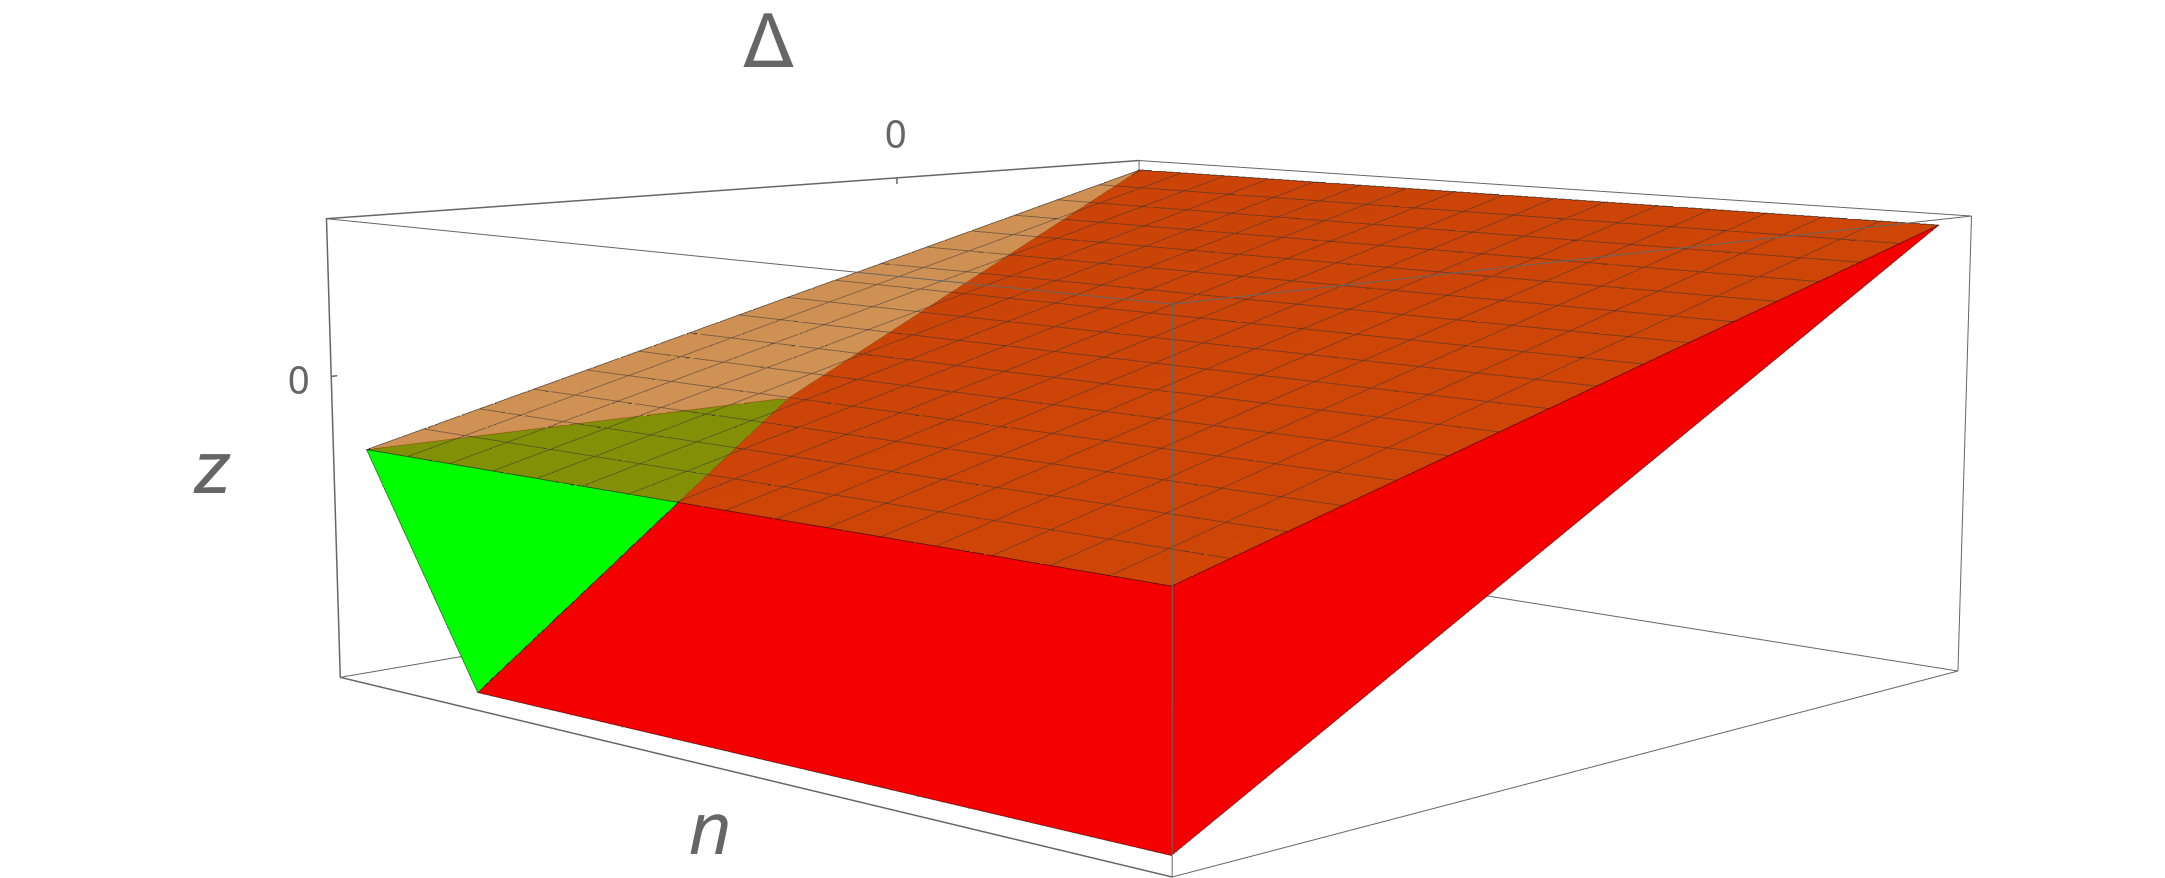
\includegraphics[width=\linewidth]{neurodiff/figs/specialcase1.png}
		\caption{Tighter upper bounding plane.}
		\label{neurodiff:fig:specialcase1}
	\end{minipage}%
	%
	\hspace{0.09\linewidth}
	%
	\begin{minipage}[t]{0.45\linewidth}
		\centering
		%\captionsetup{width=0.98\textwidth}
		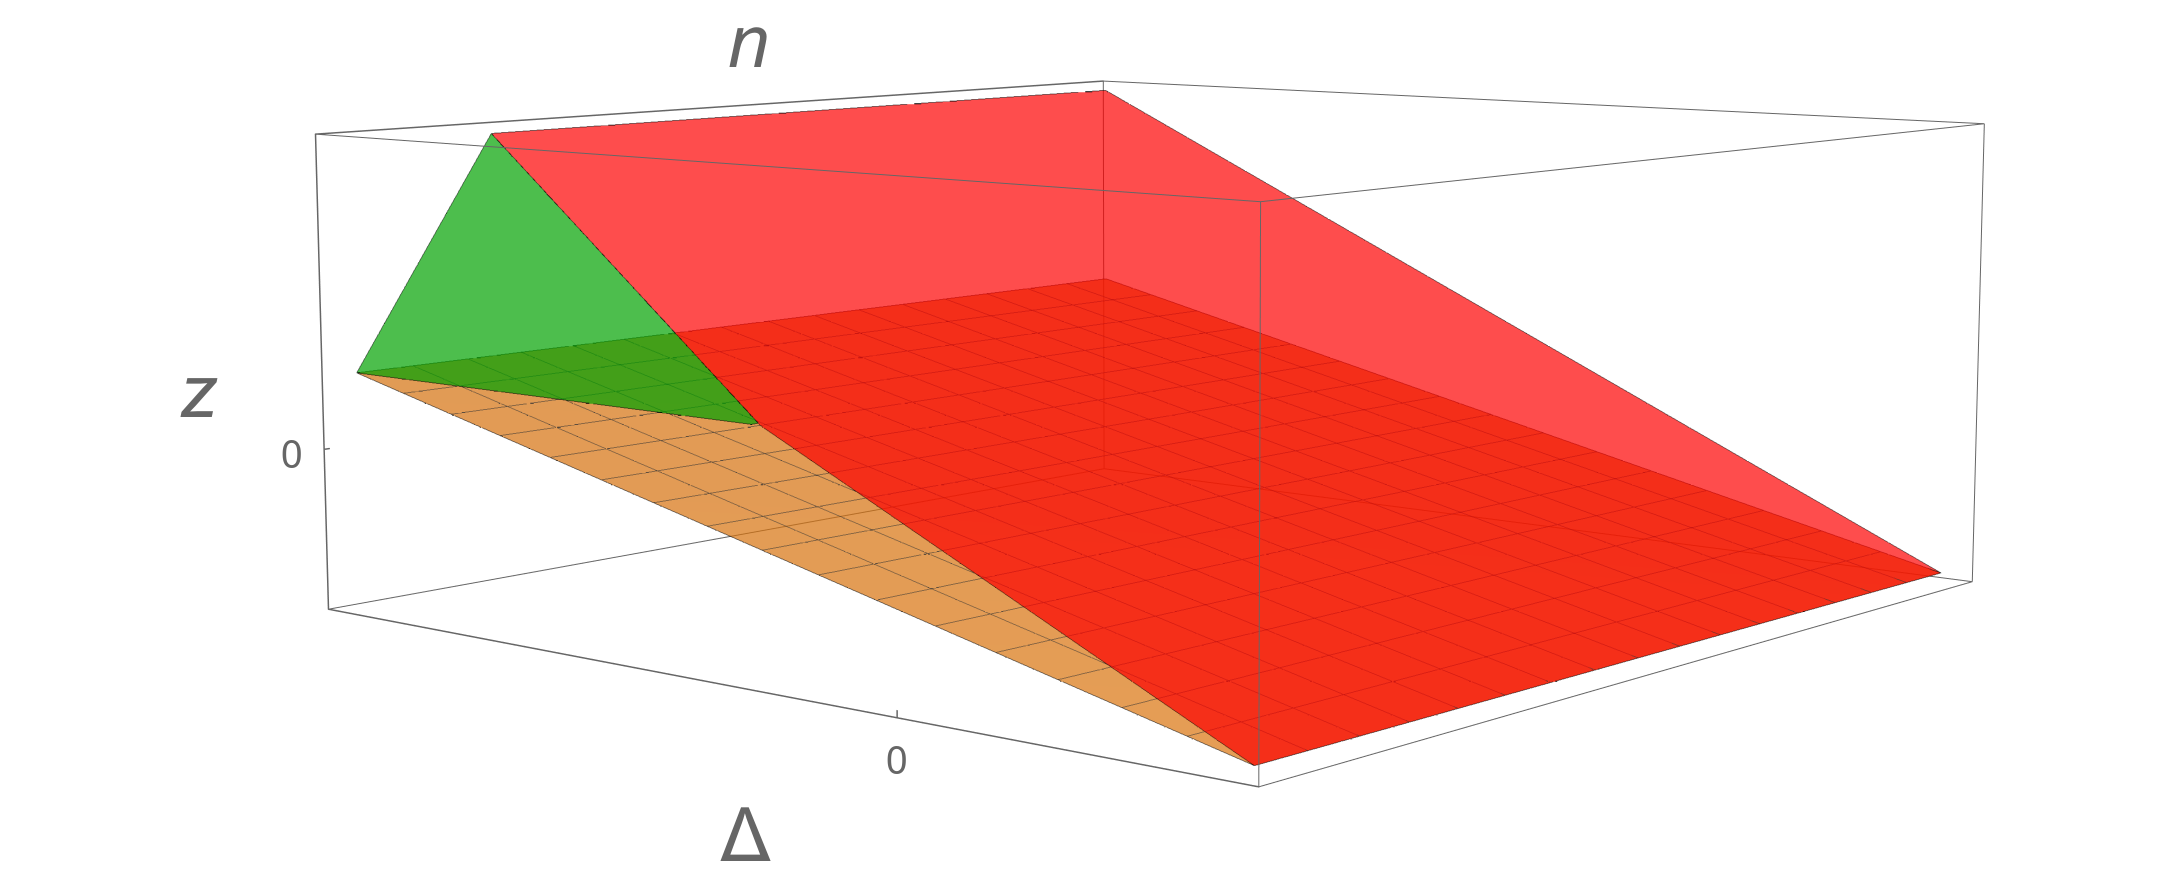
\includegraphics[width=\linewidth]{neurodiff/figs/specialcase2.png}
		\caption{Tighter lower bounding plane.}
		\label{neurodiff:fig:specialcase2}
	\end{minipage}
\end{figure*}
%
%\begin{figure}
%	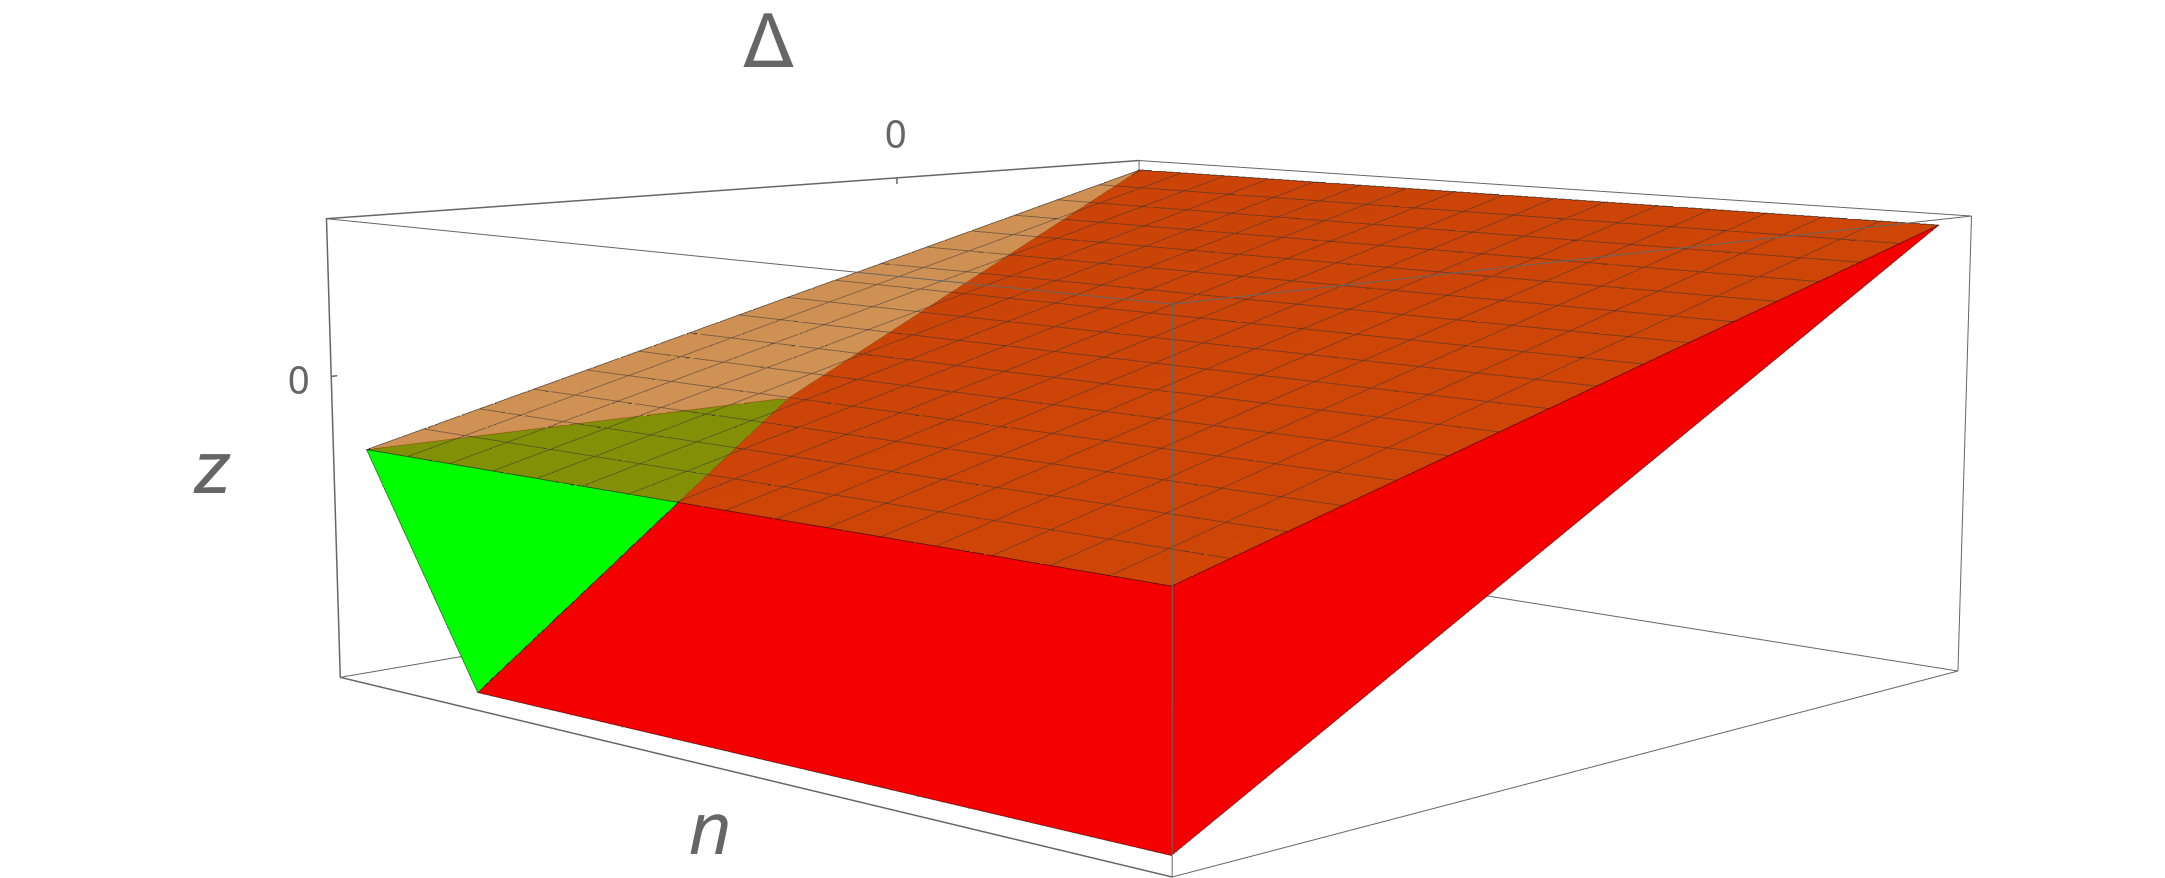
\includegraphics[width=\linewidth]{neurodiff/figs/specialcase1.png}
%	\caption{Tighter upper bounding plane.\label{neurodiff:fig:specialcase1}}
%\end{figure}
%
%\begin{figure}
%	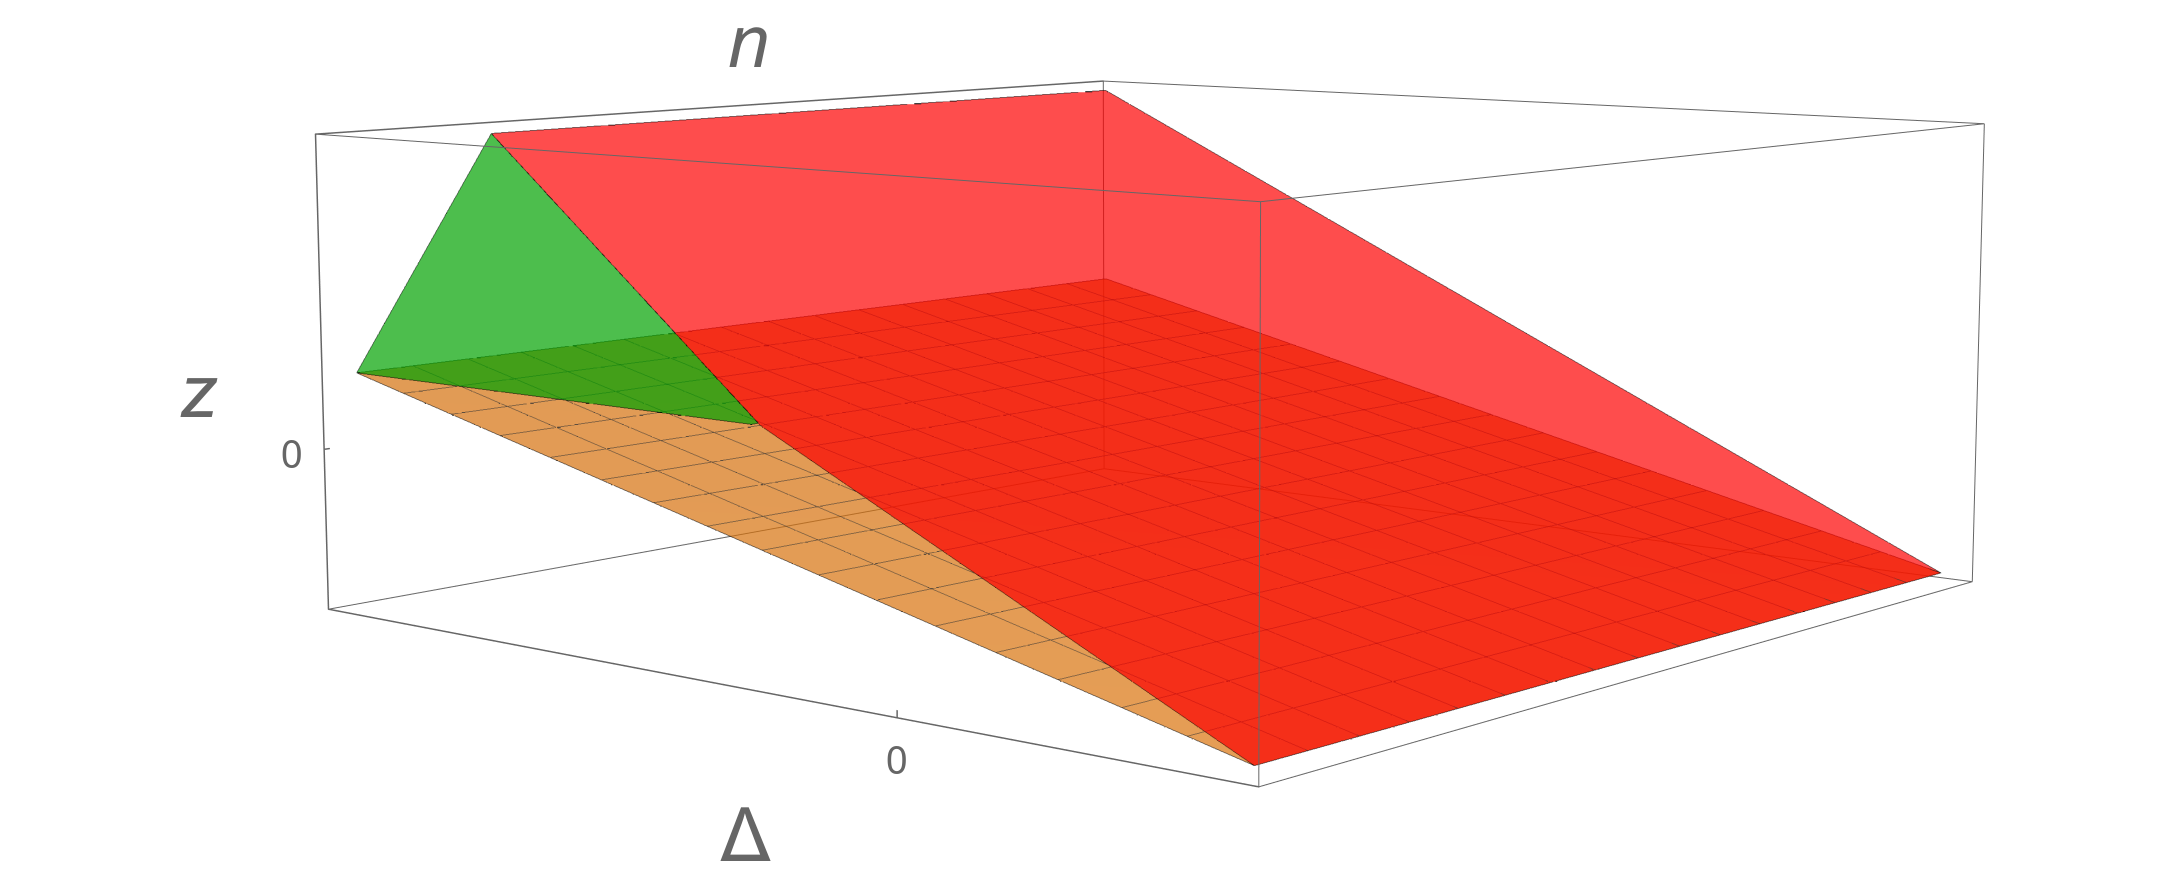
\includegraphics[width=\linewidth]{neurodiff/figs/specialcase2.png}
%	\caption{Tighter lower bounding plane.\label{neurodiff:fig:specialcase2}}
%\end{figure}

\paragraph{Tighter Upper Bound When $ \nn $ Is Linear, $ \UBL{\IntIn{\nnd}}
\leq $  $-\LBL{\IntIn{\nn}} $ $ \leq \UBU{\IntIn{\nnd}} $.}
We illustrate the $ z_1 $ plane under these constraints in
Figure~\ref{neurodiff:fig:specialcase1}.
Let $ l = \UBL{\IntIn{\nnd}} $, and let $ u = \UBU{\IntIn{\nnd}} $, and $ l' =
-\LBL{\IntIn{\nn}} $, we use Lemma~\ref{neurodiff:lemma:1} to derive
$ \UBEq{\IntOut{\nnd}} =$ $ (\UBEq{\IntIn{\nnd}} - l)*\frac{u - l'}{u
- l} + l' $. This results in the upper plane of
Figure~\ref{neurodiff:fig:specialcase1}.
This improves over the third case in our general upper
bound because it allows the lower bound of $ \UBEq{\IntOut{\nnd}} $ to
be less than 0.

\begin{proof}
By our case assumption, Equation~\ref{neurodiff:eq:1} simplifies to the one in
Lemma~\ref{neurodiff:lemma:prev1}. By Lemma~\ref{neurodiff:lemma:1}, we have for
all $ x \in X $,
$ \UBEq{\IntOut{\nnd}}(x) \geq -\LBL{\IntIn{\nn}} $ and
$ \UBEq{\IntOut{\nnd}}(x) \geq \UBEq{\IntIn{\nnd}}(x) $. These two inequalities
imply $ \UBEq{\IntOut{\nnd}} \geq max(-\nn, \nnd) $.
\end{proof}

\paragraph{Tighter Lower Bound When $ \nn $ Is Linear.}

We can use the approximation $ \LBEq{\IntOut{\nnd}}
= \LBEq{\IntIn{\nnd}} $. This improves over the second and third cases
of our general lower bound.

\begin{proof}
By our case assumption, Equation~\ref{neurodiff:eq:1} simplifies to the one in
Lemma~\ref{neurodiff:lemma:prev1}. Thus, $ z_1 = max(-\nn, \nnd) $ $ \implies $
$ z_1 \geq \nnd $.
\end{proof}

\paragraph{Tighter Lower Bound when $ \nnp $ is Linear, $ \LBL{\IntIn{\nnd}}
$ $ \leq \LBL{\IntIn{\nnp}} $ $ \leq \LBU{\IntIn{\nnd}}$.}
We illustrate the $ z_2 $ plane under these constraints in
Figure~\ref{neurodiff:fig:specialcase2}.
Here, letting $ l = \LBL{\IntIn{\nnd}} $, $ u = \LBU{\IntIn{\nnd}} $,
and $ u' = \LBL{\IntIn{\nnp}} $, we can use Lemma~\ref{neurodiff:lemma:2} to
derive the approximation $ \LBEq{\IntOut{\nnd}} $ $ =
(\LBEq{\IntIn{\nnd}} - u)*\frac{u - l'}{u - l} + u' $. This results in the
lower plane of Figure~\ref{neurodiff:fig:specialcase2}. This improves
over the third case, since it allows the upper bound to be greater
than 0.

\begin{proof}
By our case assumption, Equation~\ref{neurodiff:eq:2} simplifies to the one shown
in
Lemma~\ref{neurodiff:lemma:prev2}. By Lemma~\ref{neurodiff:lemma:2}, we have for
all $ x \in X $,
$ \LBEq{\IntOut{\nnd}}(x) \leq \LBEq{\IntIn{\nnd}}(x) $ and
$ \LBEq{\IntOut{\nnd}}(x) \leq \LBL{\IntIn{\nnp}} $. These two inequalities
imply
$ \LBEq{\IntOut{\nnd}}(x)$ $ \leq min(\nnp, \nnd) $.
\end{proof}


\subsection{Intermediate Symbolic Variables for $\IntOut{\nnd}$}
\label{neurodiff:sec:symbolic}


While convex approximations reduce the error introduced by ReLU, even
small errors tend to be amplified significantly after a few layers.
To combat the error explosion, we introduce new symbolic terms to represent the
output values of unstable neurons, which allow their accumulated
errors to cancel out.


We illustrate the impact of symbolic variables on $ \n{1}{1} $ of our
motivating example. Recall we have $ \IntOut{\nd{1}{1}} =$$ [0.05x_1 -
0.05x_2 - 0.2,$ $ 0.05x_1 - 0.05x_2 + 0.2] $. After applying the
convex approximation, we introduce a new variable $ x_3$
such that $ x_3 = $ $ [0.05x_1 - 0.05x_2 - 0.2, $ $
0.05x_1 - 0.05x_2 + 0.2 ]$.
Then we set $ \IntOut{\nd{1}{1}} = [x_3, x_3] $, and
propagate this interval as before. After propagating through
$ \n{2}{1} $ and $ \n{2}{2} $ and combining them at $ \n{3}{1} $, the
$ x_3 $ terms partially cancel out, resulting in the tighter final
output interval $ [-1.65, 1.18] $.

In principle, symbolic variables may be introduced at any unstable
neurons that introduce approximation errors,
however there are efficiency vs. accuracy tradeoffs when
introducing these symbolic variables.  One consideration
is how to deal with intermediate variables referencing other
intermediate variables. For example, if we decide to introduce a
variable $ x_4 $ for $ \n{2}{1} $, then $ x_4 $ will have an $ x_3 $
term in its equation. Then, when we are evaluating a symbolic bound that
contains
an $ x_4 $ term, which will be the case for $ \n{3}{1} $, we will have to
recursively substitute the bounds of the
previous intermediate variables, such as $ x_3 $. This becomes expensive,
especially when it is used together with our bisection-based
refinement~\cite{WangPWYJ18,paulsen2020reludiff}.
%
Thus, in practice, we first remove any back-references to intermediate
variables by substituting in their lower bounds and upper bounds into the
new intermediate variable's lower and upper bounds, respectively.

Given that we do not allow back-references, there are two
additional considerations.
%
First, we must consider that introducing a new intermediate
variable wipes out all the other intermediate variables.  For
example, introducing a new variable at $ \n{2}{1} $ wipes out references
to $ x_3 $, thus preventing any $ x_3 $ terms from canceling at $ \n{3}{1} $.
%
Second, the runtime cost of introducing symbolic variables is not
negligible. The bulk of computation time in \Name{} is spent
multiplying the network's weight matrices by the neuron's symbolic
bound equations, which is implemented using matrix multiplication. Since adding
variables increases the matrix size, this increases the matrix
multiplication cost.

Based on these considerations, we have developed heuristics for adding
new variables judiciously.
%
First, since the errors introduced by unstable neurons in
the \emph{earliest} layers are the most prone to explode, and hence
benefit the most when we create variables for them, we
rank them higher when choosing where to add symbolic variables.
%
Second, we bound the total number of symbolic variables that may be
added, since our experience shows that introducing symbolic variables
for the earliest $ N $ unstable neurons gives drastic improvements in
both run time and accuracy.
%
In practice, $N$ is set to a number proportional
to the weighted sum of unstable neurons in all layers. Formally,
$N=\Sigma_{k=1}^L \gamma^k \times N_k$, where $N_k$ is the number of
unstable neurons in layer $k$ and $\gamma^k = \frac{1}{k}$ is the discount
factor.
%
%\cwnote{Seriously, we have to fix $N$ in our tool, one way or
%another.  The reason is becuase changing $N$ for each benchmark
%arbitrarily sounds really bad!}



\section{Experiments}
\label{neurodiff:sec:experiment}

% Experiments we want to cover
% - ACAS
% 	- eps = 0.05, 0.01
%	- One big table or two small tables
% - MNIST
% 	- 4x1024
%		- increasing perturbation
%		- increasing number of pixels
%		- accuracy on perturb = 8
%	- 6x500
%		- increasing perturbation
%	- Have one line graph for increasing perturbs on both arches
%	- Also do an accuracy comparison for both arches

We have implemented \Name{} and compared it
with \ReluDiff{}~\cite{paulsen2020reludiff}, the state-of-the-art tool for
differential verification of neural networks.
%
\Name{} builds upon the codebase of \ReluDiff{}~\cite{reludiffrepo},
which was also used by single-network verification tools such
as \ReluVal{}~\cite{WangPWYJ18} and \Neurify{}~\cite{WangPWYJ18nips}.
All use OpenBLAS~\cite{ZhangWZ12} to optimize the symbolic
interval arithmetic (namely in applying the weight matrices to the
symbolic intervals).
%
We note that \Name{} uses the algorithm from \Neurify{} to compute
$ \IntOut{\nj} $ and $ \IntOut{\npj} $, whereas \ReluDiff{} uses
the algorithm of \ReluVal{}. Since \Neurify{} is known to compute
tighter bounds than \ReluVal{}~\cite{WangPWYJ18nips},
we compare to both \ReluDiff{}, and an upgraded version of \ReluDiff{}
which uses the bounds from \Neurify{} to ensure
that any performance gain is due to our optimizations and not due to
using \Neurify{}'s bounds. We use the name \ReluDiffP{} to refer
to \ReluDiff{} upgraded with \Neurify{}'s bounds.
%We also
%improved \ReluDiff{} to use a more accurate algorithm for computing
%the absolute values: the original \ReluDiff{} uses the algorithm
%from \ReluVal{}~\cite{WangPWYJ18} to compute $ \IntOut{\nj} $ and
%$ \IntOut{\npj} $, whereas the improved \ReluDiff{} uses the more
%accurate algorithm from \Neurify{}~\cite{WangPWYJ18nips}.
%
%Since our \Name{} also uses the more accurate algorithm
%from \Neurify{}, upgrading \ReluDiff{} to \ReluDiffP{} (the new
%version) allows us to have a more fair experimental comparison.


%To sum up, both \ReluDiff{}/\ReluDiffP{} and \Name{} take two
%structurally similiar networks $ f $ and $ f' $, an input region $ X
%$, and a small $ \epsilon $ value. They then attempt to prove that
%$ \forall x \in X$. $|f'(x) - f(x)| < \epsilon $ for each of the
%network's output nodes.


\subsection{Benchmarks}

Our benchmarks consist of the 49 feed-forward neural networks used by
Paulsen et al.~\cite{paulsen2020reludiff}, taken from three applications:
aircraft collision avoidance, image classification, and human activity
recognition. We briefly describe them here. As in Paulsen et
al.~\cite{paulsen2020reludiff}, the second
network $ f' $ is generated by truncating the edge weights of $f$ from
32 bit to 16 bit floats.

\paragraph{ACAS Xu~\cite{JulianKO18}}
ACAS (aircraft collision avoidance system) Xu is a set of
forty-five neural networks, each with five inputs, six hidden layers of 50 units each, and five outputs,
designed to advise a pilot (the ownship) how to steer an aircraft in the presence of an intruder aircraft.
The inputs describe the position and speed of the intruder relative to the ownship, and the
outputs represent scores for different actions that the ownship should take.
The scores range from $ [-0.5, 0.5] $. We use the input regions defined by the properties of previous
work~\cite{KatzBDJK17, WangPWYJ18}.

\paragraph{MNIST~\cite{LecunBBH98}}
MNIST is a standard image classification task, where the goal is to
correctly classify $ 28 \times 28 $ pixel greyscale images of handwritten
digits. Neural networks trained for this task take 784 inputs (one for
each pixel) each in the range $ [0,255] $, and compute ten outputs -- one
score for each of the ten possible digits. We use three networks of size
3x100 (three hidden layers of 100 neurons each), 2x512, and 4x1024 taken from Weng et al.~\cite{WengZCSHDBD18} and
Wang et al.\cite{WangPWYJ18nips}. All achieve at least 95\% accuracy on
holdout test data.

\paragraph{Human Activity Recognition (HAR)~\cite{AnguitaHAR}}
The goal for this task is to classify
the current activity of human (e.g. walking, sitting, laying down) based
on statistics from a smartphone's gyroscopic sensors. Networks trained
on this task take 561 statistics computed from the sensors and output six
scores for six different activities. We use a 1x500 network.

\subsection{Experimental Setup}

Our experiments aim to answer the following research questions:

\begin{enumerate}
	\item Is \Name{} significantly faster than state-of-the-art?
	\item Is \Name{}'s forward pass significantly more accurate?
	\item Can \Name{} handle significantly larger input regions?
	\item How much does each technique contribute to the overall improvement?
\end{enumerate}

To answer these questions, we run both \Name{}
and \ReluDiff{}/\ReluDiffP{} on all benchmarks and compare their
results.  Both \Name{} and \ReluDiff{}/\ReluDiffP{} can be
parallelized to use multithreading, so we configure a maximum of 12
threads for all experiments.  Our experiments are run on a computer
with an AMD Ryzen Threadripper 2950X 16-core processor, with a
30-minute timeout per differential verification task.


While we could try and adapt a single-network verification tool to our
task as done previously~\cite{paulsen2020reludiff}, we note that \ReluDiff{}
has been shown to significantly outperform (by several orders of
magnitude) this naive approach.



\subsection{Results}

In the remainder of this section, we present our experimental results
in two steps.  First, we present the overall verification results on
all benchmarks. Then, we focus on the detailed verification results on
the more difficult verification tasks.


\subsubsection{Summary of Results on All Benchmarks}


Our experimental results show that, on all benchmarks, the
improved \ReluDiffP{} slightly but consistently outperforms the
original \ReluDiff{} due to its use of the more accurate component
from \Neurify{} instead of \ReluVal{} for bounding the absolute values
of individual neurons.  Thus, to save space, we will only show the
results that compare \Name{} (our method) and \ReluDiffP{}.


\begin{figure}
\centering
\includegraphics[width=0.7\linewidth]{neurodiff/figs/exp_summary.png}
\caption{Comparing the execution times of \Name{} and \ReluDiffP{} on all verification tasks.}
\label{neurodiff:fig:expsummary}
\end{figure}


We summarize the comparison between \Name{} and \ReluDiffP{} using a
scatter plot in Figure~\ref{neurodiff:fig:expsummary}, where each point
represents a differential verification task: the x-axis is the
execution time of \Name{} in seconds, and the y-axis the execution
time of \ReluDiffP{} in seconds.  Thus, points on the diagonal line
are ties, while points above the diagonal line are wins for \Name{}.


The results show that \Name{} outperformed \ReluDiffP{} for most
verification tasks.  Since the execution time is in logrithmic scale
 the speedups of \Name{} are more
than 1000X for many of these verification tasks.
%
While there are cases where \Name{} is slower than \ReluDiffP{}, due
to the overhead of adding symbolic variables, the differences are on the
order of seconds.  Since they are all on the small MNIST networks and the
HAR network that are very easy for both tools, we omit
an in-depth analysis of them.


In the remainder of this section, we present an in-depth analysis of
the more difficult verification tasks.



\subsubsection{Results on ACAS Networks}


\begin{table}
	\centering
\caption{Results for ACAS networks with $ \epsilon = 0.05 $.}
\label{neurodiff:tbl:acas_orig}
		\begin{tabular}{|c|ccc|ccc|c|}\hline
			\multirow{2}{*}{\makecell[c]{Property}} &  \multicolumn{3}{c|}{\Name{} (new)}
			& \multicolumn{3}{c|}{\ReluDiffP{}} & \multirow{2}{*}{Speedup} \\
			\cline{2-7}
			& proved  & undet. & time (s) & proved & undet. & time (s) &  \\\hline
			\hline

        $\varphi_{1}$   & 45    & 0     & 522.6         & 44    & 1     & 4800.6        &   9.2         \\\hline
$\varphi_{3}$   & 42    & 0     &   2.3         & 42    & 0     &   4.1         &   1.8         \\\hline
$\varphi_{4}$   & 42    & 0     &   1.7         & 42    & 0     &   2.8         &   1.7         \\\hline
$\varphi_{5}$   & 1     & 0     &   0.2         & 1     & 0     &   0.2         &   1.4         \\\hline
$\varphi_{6}$  & 2     & 0     &   0.6         & 2     & 0     &   0.4         &   0.7         \\\hline
$\varphi_{7}$   & 1     & 0     & 1404.4        & 0     & 1     & 1800.0        &   1.3         \\\hline
$\varphi_{8}$   & 1     & 0     & 132.2         & 1     & 0     & 361.8         &   2.7         \\\hline
$\varphi_{9}$   & 1     & 0     &   0.6         & 1     & 0     &   2.3         &   3.7         \\\hline
$\varphi_{10}$  & 1     & 0     &   0.9         & 1     & 0     &   0.7         &   0.8         \\\hline
$\varphi_{11}$  & 1     & 0     &   0.2         & 1     & 0     &   0.3         &   1.6         \\\hline
$\varphi_{12}$  & 1     & 0     &   2.8         & 1     & 0     & 360.9         & 129.4         \\\hline
$\varphi_{13}$  & 1     & 0     &   5.8         & 1     & 0     &   5.1         &   0.9         \\\hline
$\varphi_{14}$  & 2     & 0     &   0.5         & 2     & 0     &  95.9         & 196.2         \\\hline
$\varphi_{15}$  & 2     & 0     &   0.6         & 2     & 0     &  65.0         & 113.2         \\\hline

		\end{tabular}
\end{table}

\begin{table}
	\centering
\caption{Results for ACAS networks with $ \epsilon = 0.01 $.}
\label{neurodiff:tbl:acas_new}
		\begin{tabular}{|c|ccc|ccc|c|}\hline
			\multirow{2}{*}{\makecell[c]{Property}} &  \multicolumn{3}{c|}{\Name{} (new)}
			& \multicolumn{3}{c|}{\ReluDiffP{}} & \multirow{2}{*}{Speedup} \\
			\cline{2-7}
			& proved  & undet. & time (s) & proved & undet. & time (s) &  \\\hline
			\hline

        $\varphi_{1}$   & 41    & 4     & 11400.1       & 15    & 30    & 55778.6       &   4.9         \\\hline
$\varphi_{3}$   & 42    & 0     &  14.3         & 35    & 7     & 13642.2       & 957.2         \\\hline
$\varphi_{4}$   & 42    & 0     &   3.8         & 37    & 5     & 9115.0        & 2390.1        \\\hline
$\varphi_{5}$   & 1     & 0     &   0.3         & 0     & 1     & 1800.0        & 5520.5        \\\hline
$\varphi_{16}$  & 2     & 0     &   1.0         & 2     & 0     &   0.8         &   0.8         \\\hline
$\varphi_{7}$   & 0     & 1     & 1800.0        & 0     & 1     & 1800.0        &   1.0         \\\hline
$\varphi_{8}$   & 1     & 0     & 1115.9        & 0     & 1     & 1800.0        &   1.6         \\\hline
$\varphi_{9}$   & 1     & 0     &   2.4         & 0     & 1     & 1800.0        & 738.2         \\\hline
$\varphi_{10}$  & 1     & 0     &   1.6         & 1     & 0     &   1.1         &   0.7         \\\hline
$\varphi_{11}$  & 1     & 0     &   0.3         & 0     & 1     & 1800.0        & 5673.8        \\\hline
$\varphi_{12}$  & 1     & 0     & 132.2         & 0     & 1     & 1800.0        &  13.6         \\\hline
$\varphi_{13}$  & 1     & 0     &  15.9         & 1     & 0     &  14.8         &   0.9         \\\hline
$\varphi_{14}$  & 2     & 0     & 1589.3        & 0     & 2     & 3600.0        &   2.3         \\\hline
$\varphi_{15}$  & 2     & 0     & 579.4         & 0     & 2     & 3600.0        &   6.2         \\\hline

		\end{tabular}
\end{table}


For ACAS networks, we consider two different sets of properties,
namely the original properties from Paulsen et al.~\cite{paulsen2020reludiff}
where $ \epsilon = 0.05 $, and the same properties but with $ \epsilon
= 0.01 $.  We emphasize that, while verifying $ \epsilon = 0.05 $ is
useful, this means that the output value can vary by up to
10\%. Considering $ \epsilon = 0.01 $ means that the output value can
vary by up to 2\%, which is much more useful.
%For all properties, we
%let \Name{} use up to 15 intermediate variables. We tuned the number
%on property $ \varphi_1 $ on the first of the 45 networks
%(i.e. network 1\_1).

Our results are shown in Tables~\ref{neurodiff:tbl:acas_orig}
and~\ref{neurodiff:tbl:acas_new}, where the first column shows the property,
which defines the input space considered. The next three columns show
the results for \Name{}, specifically the number of verified networks
(out of the 45 networks), the number of unverified networks, and the
total run time across all networks. The next three show the same
results, but for \ReluDiffP{}. The final column shows the average
speed up of \Name{}.

The results show that \Name{} makes significant gains in both speed
and accuracy. Specifically, the speedups are up to two and three
orders of magnitude for $ \epsilon = 0.05 $ and $ 0.01 $,
respectively. In addition, at the more accurate $ \epsilon = 0.01 $
level, \Name{} is able to complete 53 more verification tasks, out of
the total 142 verification tasks.


\subsubsection{Results on MNIST Networks}

\begin{figure*}[t]
\centering
	\begin{minipage}[t]{0.498\linewidth}
        \centering
		\captionsetup{width=0.9\textwidth}
		\includegraphics[width=.99\linewidth]{neurodiff/figs/4x1024_comp.png}
		\caption{Percentage of verification tasks completed on the MNIST 4x1024
		network for various perturbations.\label{neurodiff:fig:perturbation_comp}}
	\end{minipage}%
	\begin{minipage}[t]{0.498\linewidth}
        \centering
		\captionsetup{width=0.9\textwidth}
		\includegraphics[width=.99\linewidth]{neurodiff/figs/mnist_4x1024_scatterplot.png}
		\caption{Accuracy comparison for a single forward pass on the MNIST 4x1024
		network with perturbation of 8.\label{neurodiff:fig:accuracy_comp}}
	\end{minipage}%
\end{figure*}

For MNIST, we focus on the 4x1024 network, which is the largest
network considered by Paulsen et al.~\cite{paulsen2020reludiff}.  In contrast,
since the smaller networks, namely 3x100 and 2x512 networks, were
handled easily by both tools, we omit their results.
%
In the MNIST-related verification tasks, the goal is to verify
$ \epsilon = 1 $ for the given input region. We consider the two types
of input regions from the previous work, namely global perturbations
and targeted pixel perturbations, however we use input regions that
are hundreds of orders of magnitude larger.
%For all verification
%tasks, we allow 1,000 intermediate variables for \Name{}. We tuned the
%number on the first of our global perturbation properties.

First, we look at the global perturbation. For these, the input space
is created by taking an input image and then allowing a perturbation
of +/- $ p $ greyscale units to all of its pixels. In the previous
work, the largest perturbation was $ p = 3$.
%
Figure~\ref{neurodiff:fig:perturbation_comp} compares \Name{} and \ReluDiffP{}
on $ p = 3 $ all the way up to 8, where the x-axis is the perturbation
applied, and the y-axis is the percentage of verification tasks (out
of 100) that each can handle.


The results show that \Name{} can handle perturbations up to +/-
6 units, whereas \ReluDiffP{} begins to struggle at 4. While the
difference between 4 and 6, may seem small, the volume of input space
for a perturbation of 6 is $ 6^{784}/4^{784} \approx 1.1 \times
10^{138} $ times larger than 4, or in other words, 138 orders of
magnitude larger.


Next, we show a comparison of the epsilon verified by a single forward pass
for a perturbation of 8 on the MNIST 4x1024 network in
Figure~\ref{neurodiff:fig:accuracy_comp}.
Points above the blue line indicate \Name{} performed
better. Overall, \Name{} is between two and three times more accurate
than \ReluDiffP{}.

Finally, we look at the targeted pixel perturbation properties. For
these, the input space is created by taking an image, randomly
choosing $ n $ pixels, and setting there bounds to $ [0,255] $, i.e.,
allowing arbitrary changes to the chosen pixels. We again use the
4x1024 MNIST network. The results are summarized in
Table~\ref{neurodiff:tbl:MNIST_pix}. The first column shows the number of
randomly perturbed pixels. We can again see very large speedups, and a
significant increase in the size of the input region that \Name{} can
handle.


\begin{table}
	\centering
	\caption{Results of the MNIST 4x1024  pixel experiment.}
	\label{neurodiff:tbl:MNIST_pix}
	\scalebox{1.0}{
		\begin{tabular}{|c|ccc|ccc|c|}\hline
			\multirow{2}{*}{\makecell[c]{Num. \\ Pixels}} &  \multicolumn{3}{c|}{\Name{} (new)}
			& \multicolumn{3}{c|}{\ReluDiffP{}} & \multirow{2}{*}{Speedup} \\
			\cline{2-7}
			& proved  & undet. & time (s) & proved & undet. & time (s) &  \\\hline
			\hline

15      & 100   & 0     & 236.5 & 100   & 0     & 1610.2        &   6.8 \\\hline
18      & 100   & 0     & 540.8 & 88    & 12    & 34505.8       &  63.8 \\\hline
21      & 100   & 0     & 1004.0        & 30    & 70    & 145064.5      & 144.5 \\\hline
24      & 99    & 1     & 7860.1        & 1     & 99    & 179715.9      &  22.9 \\\hline
27      & 83    & 17    & 49824.0       & 0     & 100   & 180000.0      &   3.6 \\\hline


		\end{tabular}
	}
\end{table}


\subsubsection{Contribution of Each Technique}

Here, we analyze the contribution of individual techniques, namely
convex approximations and symbolic variables, to the overall
performance improvement.

%We look at the benefit in two of our experiments: the ACAS
%experiments with $ \epsilon = 0.01 $ presented in
%Table~\ref{neurodiff:tbl:acas_comp} and MNIST with varying degrees of global
%perturbations presented in Table~\ref{neurodiff:tbl:MNIST_comp}.


\begin{comment}
In Table~\ref{neurodiff:tbl:acas_comp}, we compare the performance of \Name{}
with both techniques enabled and \Name{} with only intermediate
variables. The right most column essentially shows the speedup with
the addition convex approximations. Overall we can see that the
speedup is relatively small, and that the intermediate variables do
most of the heavy-lifting in the ACAS experiments.


\begin{table}
	\caption{Comparison of full \Name{} and  \Name{} with only symbolic variables
	on ACAS experiments with $ \epsilon = 0.01 $. \label{neurodiff:tbl:acas_comp}}
	\scalebox{0.75}{
		\begin{tabular}{|c|ccc|ccc|c|}\hline
			\multirow{2}{*}{\makecell[c]{Property}} &  \multicolumn{3}{c|}{\Name{}}
			& \multicolumn{3}{c|}{Int. Vars. Only} & \multirow{2}{*}{Speedup} \\
			\cline{2-7}
			& proved  & undet. & time (s) & proved & undet. & time &  \\\hline
			\hline

			$\varphi_{1}$ 	& 40 	& 5 	& 11930.8 	& 40 	& 5 	& 12102.5 	&   1.0 	\\\hline
			$\varphi_{3}$ 	& 42 	& 0 	&  12.0 	& 42 	& 0 	&  46.8 	&   3.9 	\\\hline
			$\varphi_{4}$ 	& 42 	& 0 	&   3.4 	& 42 	& 0 	&   7.9 	&   2.3 	\\\hline
			$\varphi_{5}$ 	& 1 	& 0 	&   0.2 	& 1 	& 0 	&   0.3 	&   1.3 	\\\hline
			$\varphi_{6}$ 	& 2 	& 0 	&   0.6 	& 2 	& 0 	&   0.6 	&   1.1 	\\\hline
			$\varphi_{7}$ 	& 0 	& 1 	& 1800.0 	& 0 	& 1 	& 1800.0 	&   1.0 	\\\hline
			$\varphi_{8}$ 	& 1 	& 0 	& 756.5 	& 1 	& 0 	& 1154.9 	&   1.5 	\\\hline
			$\varphi_{9}$ 	& 1 	& 0 	&   1.8 	& 1 	& 0 	&   3.2 	&   1.8 	\\\hline
			$\varphi_{10}$ 	& 1 	& 0 	&   1.0 	& 1 	& 0 	&   1.1 	&   1.1 	\\\hline
			$\varphi_{11}$ 	& 1 	& 0 	&   0.2 	& 1 	& 0 	&   0.3 	&   1.3 	\\\hline
			$\varphi_{12}$ 	& 1 	& 0 	& 148.5 	& 1 	& 0 	& 228.3 	&   1.5 	\\\hline
			$\varphi_{13}$ 	& 1 	& 0 	&  10.6 	& 1 	& 0 	&  12.6 	&   1.2 	\\\hline
			$\varphi_{14}$ 	& 2 	& 0 	& 1798.0 	& 2 	& 0 	& 2116.3 	&   1.2 	\\\hline
			$\varphi_{15}$ 	& 2 	& 0 	& 513.3 	& 2 	& 0 	& 690.8 	&   1.3 	\\\hline

		\end{tabular}
	}
\end{table}

\end{comment}



In Table~\ref{neurodiff:tbl:MNIST_comp}, we present the average $ \epsilon $
that was able to be verified after a single forward pass on the
4x1024 MNIST network for each of
the four techniques: \ReluDiffP{} (baseline), \Name{} with only convex
approximations, \Name{} with only intermediate variables, and the
full \Name{}.


Overall, the individual benefits of the two proposed approximation
techniques are obvious.  While convex approximation
(alone) consistently provides benefit as perturbation increases, the
benefit of symbolic variables (alone) tends to decrease.
%
In addition, combining the two provides much greater benefit than the
sum of their individual contributions. With perturbation of 8, for
example, convex approximations alone are 1.59 times more accurate than
\ReluDiffP{}, and intermediate variables alone are 1.01 times more accurate.
However, together they are 2.93 times more accurate.


\begin{table}
	\centering
	\caption{Evaluating the individual contributions of convex approximation and symbolic variables using the  MNIST 4x1024 global perturbation experiment.}
	\label{neurodiff:tbl:MNIST_comp}
	\scalebox{1.0}{
		\begin{tabular}{|c|c|c|c|c|}\hline
			\multirow{2}{*}{Perturb} &  \multicolumn{4}{c|}{Average $ \epsilon $ Verified} \\
			\cline{2-5}
			& \ReluDiffP{} & Conv. Approx. & Int. Vars. & \Name{} \\
			\hline
3 & 0.59 & 0.42 (+1.39x) & 0.43 (+1.38x) & 0.20 (+2.93x) \\\hline
4 & 1.02 & 0.70 (+1.46x) & 0.87 (+1.18x) & 0.36 (+2.85x) \\\hline
5 & 1.60 & 1.06 (+1.52x) & 1.47 (+1.09x) & 0.56 (+2.87x) \\\hline
6 & 2.29 & 1.47 (+1.55x) & 2.19 (+1.04x) & 0.79 (+2.90x) \\\hline
7 & 3.02 & 1.92 (+1.58x) & 2.96 (+1.02x) & 1.04 (+2.91x) \\\hline
8 & 3.80 & 2.39 (+1.59x) & 3.77 (+1.01x) & 1.30 (+2.93x) \\\hline
		\end{tabular}
	}
\end{table}


The results suggest two things.
%
First, intermediate
symbolic variables perform well when a significant portion of the
network is already in the stable state.  We confirm, by manually
inspecting the experimental results, that it is indeed the case when
we use a perturbation of 3 and 8 in the MNIST experiments.
%, and we believe
%this is the case for ACAS as well, once the input space is
%sufficiently partitioned.
Second, the convex approximations provide the most benefit when the
pre-ReLU delta intervals are (1) significantly wide, and (2) still
contain a significant amount of symbolic information. This is also
confirmed by manually inspecting our MNIST results: increasing the
perturbation increases the overall width of the delta intervals.
%In
%addition, this is very likely why we do not see a significant benefit
%from convex approximations in the ACAS results. Since the ACAS
%networks have many fewer parameters than the MNIST network, the total
%amount of change in the network from rounding to 16 bits is relatively
%small. This leads to relatively narrow delta intervals, and hence
%there is little opportunity for benefit.

%\subsection{Threats to Validity}
%We note that the refinement of both \Name{} and \ReluDiff{} typically does not work well with large input spaces. However, the LP solving-based refinement of Wang et al.~\cite{WangPWYJ18nips} has been shown to scale better to higher-dimensional input spaces, and could straightforwardly be integrated into \Name{}.
%
%We also focus on feed-forward ReLU networks. ReLU activations are preferable in safety critical systems because they are the most amenable to verification. Still, much previous work~\cite{SinghGPV19, SinghGPV19iclr, zhang2018efficient} has shown that convex approximations can be extended non-linear activations as well. We believe \Name{} can be extended as such too.


%\section{Related Work}
%\label{neurodiff:sec:related}
%
%
%% Single network verification
%% - complete techniques
%Aside from \ReluDiff{}~\cite{paulsen2020reludiff}, the most closely related to
%our work are those that focus on verifying properties of single
%networks as opposed to two or more networks. These verification
%approaches can be broadly categorized into those that use exact,
%constraint solving-based techniques and those that use approximations.
%
%
%On the constraint solving side, several works have adapted
%off-the-shelf solvers~\cite{CarliniW17, tjeng2019evaluating,
%BastaniILVNC16, Ehlers17, baluta2019quantitative}, or even implemented
%solvers specifically for neural networks~\cite{KatzBDJK17,
%KatzHIJLLSTWZDK19}.
%%
%On the approximation side, many use techniques that fit into the framework of
%abstract interpretation~\cite{CousotC77}. For example, many works have leveraged
%abstract domains such as intervals~\cite{WangPWYJ18, WengZCSHDBD18,
%zhang2018efficient, JulianKO18}, polyhedra~\cite{Singh2019krelu, SinghGPV19}, and
%zonotopes~\cite{SinghGPV19iclr, GehrMDTCV18}.
%
%
%In addition, these verification techniques have also been
%combined~\cite{SinghGPV19iclr, WangPWYJ18nips, HuangKWW17}, or
%entirely different approaches~\cite{RuanHK18, DvijothamSGMK18,
%GopinathKPB18}, such as bounding a network's lipschitz constant, have
%been studied. These verification techniques can also be integrated
%into the training process to produce more robust and easier to verify
%networks~\cite{FischerBDGZV19, MirmanGV18, WongK18,
%balunovic2020adversarial}. These works are orthogonal, though we
%believe their techniques can be adapted to our domain.
%
%
%% Various heuristic based approaches, focus on discovering but not proving the
%%absence of adversarial examples
%A related but tangential line of work focuses on discovering
%interesting behaviors of neural networks, though without any
%guarantees.
%%
%Most closely related to our work are differential testing
%techniques~\cite{xie2019diffchaser, PeiCYJ17, MaLLZG18}, which focus
%on finding disagreements between a set of networks.
%%
%However, these techniques do not attempt to prove the equivalence or
%similarity of multiple networks.
%
%Other works are more geared towards single network testing, and use
%white-box testing techniques~\cite{ma2018deepgauge, xie2019deephunter,
%SunWRHKK18, TianPJR18, odena2018tensorfuzz}, such as neuron coverage
%statistics, to assess how well a network has been tested, and also
%report interesting behaviors. Both of these can be thought of as
%adapting software engineering techniques to machine learning.
%
%
%In addition, many works use machine learning techniques, such as
%gradient optimization, to find interesting behaviors, such as
%adversarial examples\cite{KurakinGB17a, madry2017towards, NguyenYC15,
%XuQE16, Moosavi-Dezfooli16}. These interesting behaviors can then be
%used to retrain the network to improve
%robustness~\cite{GoodfellowSS15, RaghunathanSL18}. Again, these
%techniques do not provide guarantees, though we believe they could be
%integrated into \Name{} to quickly find counterexamples.
%
%Finally, our work draws inspiration from classic software engineering
%techniques, such as regression testing~\cite{rothermel1997safe},
%differential assertion checking~\cite{lahiri2013differential},
%differential fuzzing~\cite{NilizadehNP19}, and incremental symbolic
%execution~\cite{Person11,GuoKW16}, where one version of a program is
%used as an ``oracle'', to more efficiently test or verify a new
%version of the same program.  In our case, $ f $ can be thought of as
%the oracle, while $ f' $ is the new version.


\section{Summary}
\label{neurodiff:sec:conclusion}

We have presented \Name{}, a scalable differential verification
technique for soundly bounding the difference between two feed-forward
neural networks. \Name{} leverages novel convex approximations, which
reduce the overall approximation error, and intermediate symbolic
variables, which control the error explosion, to significantly improve
efficiency and accuracy of the analysis. Our experimental evaluation
shows that \Name{} can achieve up to 1000X speedup and is up to five
times as accurate.




\chapter{Online Synthesis of Linear Approximations}
\label{ch:onlinesyn}
\newcommand\bpnote[1]{\textcolor{blue}{{\textbf{Brandon Says: #1}}}}
\declarecommand\jwnote[1]{\textcolor{purple}{{\textbf{Jingbo Says: #1}}}}
\declarecommand\cwnote[1]{\textcolor{red}{{\textbf{Chao Says: #1}}}}

\declarecommand{\Name}{\textsc{LinSyn}}
\declarecommand{\ReluDiff}{\textsc{ReluDiff}}
\declarecommand{\ReluVal}{\textsc{ReluVal}}
\declarecommand{\DeepPoly}{\textsc{DeepPoly}}
\declarecommand{\Reluplex}{\textsc{Reluplex}}
\declarecommand{\Neurify}{\textsc{Neurify}}
\declarecommand{\Crown}{\textsc{Crown}}
\declarecommand{\Popqorn}{\textsc{Popqorn}}
\declarecommand{\RefineZono}{\textsc{RefineZono}}
\declarecommand{\dReal}{\textsc{dReal}}
\declarecommand{\autolipra}{\textsc{AutoLiRPA}}
\declarecommand{\popqorn}{\textsc{POPQORN}}

\declarecommand{\nj}[0]{n_{k,j}}
\declarecommand{\n}[2]{n_{#1,#2}}
\declarecommand{\np}[2]{n'_{#1,#2}}
\declarecommand{\npj}[0]{n'_{k,j}}
\declarecommand{\nd}[2]{\Delta_{#1,#2}}
\declarecommand{\ndj}{\Delta_{k,j}}
\declarecommand{\W}[3]{W_{#1}[#2,#3]}
\declarecommand{\Wp}[3]{W_{#1}'[#2,#3]}
\declarecommand{\Wk}[1]{W_{#1}}
\declarecommand{\Wd}[3]{W_{#1}^\Delta[#2,#3]}

%\subsubsection{\textcolor{red}{There is a need for verifying the robustness of
%neural network...}}
Prior work has shown that neural networks are vulnerable to various types of
(adversarial) perturbations, such as small $l$-norm bounded
perturbations~\cite{szegedy2013intriguing}, geometric
transformations~\cite{engstrom2019exploring,kanbak2018geometric}, and word
substitutions~\cite{alzantot2018generating}. Such perturbations can often
cause a misclassification for any given input, which may have serious
consequences, especially in safety critical systems.
%
Certifying robustness to these perturbations has become an important problem as
it can show the network does not exhibit these misclassifications, and
furthermore
previous work has shown that a given input feature's
certified robustness can be a useful indicator to determine the feature's
importance in the network's decision~\cite{shi2020robustness,ko2019popqorn}.

%\subsubsection{\textcolor{red}{The most scalable approach relies on computing
%symbolic ranges}}
Indeed, many approaches have been proposed for certifying the
robustness of inputs to these perturbations. Previous work typically
leverages two types of techniques: (1) fast and scalable, but approximate
techniques~\cite{SinghGPV19,GehrMDTCV18,WengZCSHDBD18,shi2020robustness,ko2019popqorn},
 and (2) expensive but exact techniques that leverage some type of
constraint
solver~\cite{KatzBDJK17,KatzHIJLLSTWZDK19,tjeng2019evaluating}. Several works
have also
combined the
two~\cite{SinghGPV19iclr,Singh2019krelu,WangPWYJ18nips,tran2019star}. The
most successful approaches, in terms of scalability in practice, are built on top of the approximate techniques, which
all depend on computing \textit{linear bounds} for the non-linear activation functions.

%\begin{itemize}
%\item don't forget to cite papers such as ReluPlex
%\item don't forget to cite papers such as ReluVal and DeepPoly
%\item cite other important papers as well
%\end{itemize}

%\subsubsection{\textcolor{red}{However, existing techniques for computing the
%linear bounds have limitations}}

However, a key limitation is that the linear bounds must be handcrafted and
proven sound by experts. Not only is this process difficult, but also ensuring
the tightness of the crafted bounds presents an additional challenge.
Unfortunately, prior work has only crafted bounds for the most common
activation functions and architectures, namely ReLU~\cite{WangPWYJ18nips},
sigmoid, tanh~\cite{SinghGPV19,zhang2018efficient,wu2021tightening}, the exp
function~\cite{shi2020robustness}, and some
2-dimensional activations found in LSTM networks~\cite{ko2019popqorn}.
%
As a result, existing tools for neural network verification
cannot handle a large number of activation functions that are
frequently used in practice.  Examples include the \emph{GELU}
function~\cite{hendrycks2016gaussian}, which is currently the activation
function used in OpenAI's GPT~\cite{radford2018improving}, and the \emph{Swish}
function which has been shown to outperform the standard ReLU function in some
applications~\cite{ramachandran2017searching} and, in particular, can reduce
over-fitting in adversarial training~\cite{singla2021low}. In addition, these
recently introduced activation
functions are often significantly more complex than previous activation
functions, e.g., we have $
\mathit{gelu}(x) = 0.5 x ( 1 + \tanh{[ \sqrt{2 / \pi } (x + 0.044715x ^{3} ) ]
} )
$.
%
%In addition, even for activation functions that can be handled by
%existing tools, many of the hand-crafted bounds are suboptimal and/or
%do not come with tightness guarantees.

%\begin{itemize}
%	\item They require linear bounds to be provided by experts
%	\item The bounds can be difficult to craft, e.g. the best known bounds for
%LSTM activations are heuristic
%    \item They are often sub-optimal, i.e., these bounds are not tight enough
%\end{itemize}

%\subsubsection{\textcolor{red}{Problem statement}}



%TODO:
% - change to z = sigma(x)
% - change n to d
In this work, we study the problem of \textit{efficiently} and
\textit{automatically}
synthesizing \textit{sound} and \textit{tight} linear bounds for any
\textit{arbitrary activation function}.
%
By \emph{arbitrary activation function}, we mean \textit{any} (non-linear)
computable function $ z = \sigma(x_1,\dots,x_d) $ used inside a neural network
with $ d $ input variables.
%
By \textit{sound} we mean, given an interval bound on each
variable $ x_1 \in
[l_1, u_1], x_2 \in [l_2, u_2], \dots, x_d \in [l_d, u_d]$, the problem is to \textit{efficiently}
compute lower bound coefficients $ c^l_1, c^l_2, \dots, c^l_{d+1} $, and upper
bound coefficients $ c^u_1, c^u_2, \dots, c^u_{d+1} $ such that the following
holds:
\begin{equation}\label{onlinesyn:eq:intro-sound}
\begin{gathered}
	\forall x_1 \in [l_1, u_1], x_2 \in [l_2, u_2], \dots,  x_d \in [l_d, u_d]\\
	c^l_1x_1 + c^l_2x_2 + \dots + c^l_{d+1}
	\leq \sigma(x_1,\dots,x_d) \leq
	c^u_1x_1 + c^u_2x_2 + \dots + c^u_{d+1}
\end{gathered}
\end{equation}
%
By \textit{automatically}, we mean that the above is done using only the
definition of the activation function itself.
%
Finally, by \textit{tight}, we mean that some formal measure, such as the
volume above/below the linear bound, is minimized/maximized.

\begin{figure}[t]
	%\textcolor{red}{We need to draw a block diagram, to illustrate the three
	%steps
	%of \Name{}.}
	%\vspace{5ex}
	%\textcolor{red}{We also need to show the input to \Name{} (defintion of
	%the
	%activation function, provided \emph{a priori}, and given input region,
	%provide
	%at run time).}
	%\vspace{5ex}
	%\textcolor{red}{Perhaps we can also show how \Name{} fits into a generic
	%verification tool (could be, but doesn't have to be, AutoLiPRA).}
	\centering
	\includegraphics[width=.9\linewidth]{onlinesyn/figs/flow_diagram.pdf}
\caption{The overall flow of~\Name{}.\label{onlinesyn:fig:block-diagram}}
\end{figure}

%\subsubsection{\textcolor{red}{High-level description of our method}}

We have developed a new method, named~\Name{}, that can \emph{automatically}
synthesize tight linear bounds for \emph{any arbitrary} non-linear activation
function $ \sigma(\cdot) $.
%
We illustrate the flow of our method on the left-hand side of
Fig.~\ref{onlinesyn:fig:block-diagram}. As shown,~\Name{} takes two inputs: a
definition of the activation function, and an interval for each of its
inputs.~\Name{} outputs linear coefficients such that
Equation~\ref{onlinesyn:eq:intro-sound} holds.
%
Internally,~\Name{}
uses sampling and an LP (linear programming) solver to synthesize
candidate lower and upper bound coefficients.
Next, it uses an
efficient local minimizer to compute a good estimate of the offset
needed to ensure soundness of the linear bounds.
%
Since the candidate bounding functions constructed in this manner may
still be unsound, finally, we use a highly optimized branch-and-bound
nonlinear SMT solver, named~\dReal{}~\cite{gao2013dreal}, to verify the
soundness of the linear bounds.
%
Even though our new method involves the use of solvers and
optimizers, the entire process typically takes less than 1/100th of a
second per pair of bounds.

Fig.~\ref{onlinesyn:fig:block-diagram} also illustrates how~\Name{} fits in with
existing neural network verification frameworks, such as ERAN~\cite{eran},
and~\autolipra{}~\cite{autolipra}. These tools take as input a neural network,
and a region of the neural networks input space, and compute an
over-approximation of the neural network's outputs. Internally, these
frameworks have modules that compute linear bounds for a specific activation
functions.~\Name{} is a one-size-fits-all drop-in replacement for these modules
that are invoked at runtime whenever a linear bound of a non-linear activation function is needed.
%Furthermore, we propose an optimization that can exploit
%convex/concave regions of $ \sigma $.

% Our approach
% - bound activation without decomposition
% - actually supports any sigma composed of computable mathematical operations
% - comes with (asymptotic) tightness guarantees

% our approach can serve as a useful comparison point for handcrafted linear
%approximations
% it can be used as a bound tightening technique



%\subsubsection{\textcolor{red}{How is it different from the problem solved by
%AutoLipra~\cite{autolipra}?}}

%\begin{wrapfigure}{R}{0.5\textwidth}
%	\centering
%	\vspace{-4ex}
%	\includegraphics[width=0.8\linewidth]{onlinesyn/figs/ours_vs_autolirpa.pdf}
%	\caption{Linear bounds for $ gelu(x) $.\label{onlinesyn:fig:boundcompare}}
%	\vspace{-2ex}
%\end{wrapfigure}

Our method differs from these existing frameworks because a user (usually an
expert in neural network verification) must provide
hand-crafted, sound linear bounds for the activation functions of a
neural network.
%
%However, to date, they only supports common activations
%like ReLU, sigmoid, tanh, and the exp function, and binary operations,
%namely addition, subtraction, multiplication, and division.
%
However, to date, they only support the previously mentioned activation
functions. We note however that the recent framework~\autolipra{} supports
binary operations (namely addition, subtraction, multiplication, and division)
as ``activation functions''. Thus, while it's not explicitly designed to handle
complex
activations, it has the ability to by decomposing, e.g., $ gelu(x) $ into
operations that it supports, and then combining them. In contrast,~\Name{}
bounds the activation function \textit{as a whole}, which we will show produces
much tighter linear bounds.
%
%Specifically, for $ \mathit{gelu}(x) $, it could first decompose $ x + x^3 $
%into $ x + x
%\times x \times x $, then bound $ x \times x $ twice, and then bound an
%addition with $ x $. It would then bound a multiplication, a $ tanh $, an
%addition, and finally two more multiplications.
%%
%We illustrate the effect of such decomposition in
%Fig.~\ref{onlinesyn:fig:boundcompare}
%by
%showing the linear bounds computed by this approach vs.~\Name{}, which does not
%perform decomposition. We can see~\Name{}'s bounds are significantly tighter
%while being fully automatic.

%While decomposing makes these frameworks applicable to a wide
%variety of network architectures and activation functions, decomposing loses
%any tightness guarantees for the activation function as a whole, and we show
%experimentally that it drastically reduces the precision of the analysis.
%This decomposition loses any tightness guarantees for $ \sigma $ as a whole,
%leading to looser bounds, and significantly reducing the precision of the
%analysis.

% lacks support for several operations and activations
% decomposing loses any guarantees on tightness




%\subsubsection{\textcolor{red}{Does it work in practice?}}

We have implemented our method in tool called \Name{}, and evaluated it on
benchmarks in computer vision and natural language processing (NLP).
Our evaluation shows that we can obtain final output bounds often 2-5X
tighter than the most general tool~\cite{autolipra}, thus allowing us to drastically
increase certified robustness.
%
In addition, our tool achieves accuracy equal to or better
than the handcrafted LSTM bounds of \Popqorn{}~\cite{ko2019popqorn}, which is
currently the most accurate tool for analyzing LSTM-based NLP models, at a
comparable runtime.



%\subsubsection{\textcolor{red}{List of the innovative claims}}

To summarize, this paper makes the following contributions:
\begin{itemize}
	\item We propose the first method for automatically synthesizing  tight linear bounds for
	arbitrary activation functions.
	\item We implement our approach in a tool called~\Name{}, and integrate it
	as a bounding module into the~\autolipra{} framework, thus producing a
	neural network verification tool that can theoretically compute tight linear
	bounds for any arbitrary activation function.
	\item We extensively evaluate our approach and show it outperforms
	state-of-the-art tools in terms of accuracy and certified robustness by a
	large margin.
\end{itemize}


The rest of this chapter is organized as follows.  First, we provide the
technical background in Section~\ref{onlinesyn:sec:preliminaries}.  Then, we
present our method for synthesizing the linear bounds in
Section~\ref{onlinesyn:sec:method-1} and our method for verifying the linear
bounds in Section~\ref{onlinesyn:sec:method-2}.  Next, we present the
experimental results in Section~\ref{onlinesyn:sec:experiment}. Finally, we
summarize the contributions of this chapter in
Section~\ref{onlinesyn:sec:conclusion}.



\section{Preliminaries}
\label{onlinesyn:sec:preliminaries}

In this section, we define the neural network verification problem, and
illustrate both how state-of-the-art verification techniques work, and their
limitations.

\subsection{Neural Networks}

%\subsubsection{introduce the canonical problem: given an input region, compute
%	an over-approximation of the output region}
%\subsubsection{this problem formulation allows us to verify all sorts of good
%	properties like robustness to L-norm perturbations}

Following conventional notation, we refer to matrices with capital bold letters
(e.g. $ \mathbf{W} \in \mathbb{R}^{n \times m}$), vectors as lower case bold
letters (e.g. $ \mathbf{x} \in \mathbb{R}^n $), and scalars or variables with
lower case letters (e.g. $ x \in \mathbb{R} $). Slightly deviating from the
convention, we refer to a set of elements with capital letters (e.g. $ X
\subseteq \mathbb{R}^n $).

We consider two types of networks in our work: feed-forward and recurrent. We
consider a feed-forward neural network to be a (highly) non-linear function $f :
\mathbb{X} \to \mathbb{Y} $, where $\mathbb{X} \subseteq \mathbb{R}^n$ and $
\mathbb{Y} \subseteq \mathbb{R}^m $. We focus on neural network
\textit{classifiers}. For an input $ \mathbf{x} \in \mathbb{X} $, each element
in the output $ f(\mathbf{x}) $ represents a score for a particular class, and
the class
associated with the largest element is the chosen class. For example, in image
classification, $ \mathbb{X} $ would be the set of all images, each element of
an input $ \mathbf{x} \in \mathbb{X} $ represents a pixel's value, and each
element in $ \mathbb{Y} $ is associated with a particular object that the image
might contain.
%We refer to each element (or dimension) of $ \mathbb{X} $ with
%the variables $ x_1, ..., x_n $, and each element of $ \mathbb{Y} $ with $
%y_1,
%..., y_m $.


In feed-forward neural networks the output $ f(\mathbf{x}) $ is computed by
performing a
series of affine transformations, i.e., multiplying by a weight matrix, followed
by application of an activation function $ \sigma(\cdot) $. Formally, a neural
network with $ l $ layers has $ l $ two-dimensional weight matrices and $ l $
one-dimensional bias vectors $ \mathbf{W_i}, \mathbf{b_i},$ where $i
\in {1..l}
$, and thus we have $ f(\mathbf{x}) = \mathbf{W_l} \cdot \sigma(\mathbf{W_{l-1}}
\dots \cdot \sigma(\mathbf{W_1} \cdot \mathbf{x} + \mathbf{b_1}) \dots +
\mathbf{b_{l-1}}) + \mathbf{b_l} $, where $ \sigma(
\cdot ) $
is the activation function applied element-wise
to the input vector. The default choice of activation is typically the
sigmoid $ \sigma(x) = 1 / (1 + e^{-x}) $, $ \tanh{} $, or ReLU
function $\sigma(x) = max(0, x) $, however recent
work~\cite{hendrycks2016gaussian,ramachandran2017searching,radford2018improving}
 has shown that functions such as $ gelu(x) $ and $ \mathit{swish}(x) = x
\times \mathit{sigmoid}(x) $ can have better performance and desirable
theoretical properties.

Unlike feed-forward neural networks, recurrent neural networks receive a
sequence of inputs $ [\mathbf{x^{(1)}}, $  $ \dots, $  $ \mathbf{x^{(t)}} ] $, and
the
final
output of $ f $ on $ \mathbf{x_t} $ is used to perform the classification of
the whole sequence. Recurrent neural networks are
\textit{state-ful}, meaning they maintain a state vector
that contains information about inputs previously given to
$ f $, which also gets updated on each call to $ f $.
%
In particular, we focus on \textit{long short-term memory} (LSTM) networks, which
have seen wide adoption in natural language processing (NLP) tasks due to their
sequential nature. For LSTMs trained for NLP tasks, the network receives a
sequence of \textit{word embeddings}. A word embedding is an $ n $-dimensional
vector that is associated with a particular word in a (natural) language. The
distance between word embeddings carries semantic significance -- two word
embeddings that are close to each other in $ \mathbb{R}^n $ typically have
similar meanings or carry a semantic relatedness (e.g. \textit{dog} and
\textit{cat} or \textit{king} and \textit{queen}), whereas unrelated words
typically are farther apart.

LSTM networks further differ from feed-forward networks in
that their internal activation functions are \textit{two}-dimensional.
Specifically, we have the following two activation patterns: $ \sigma_1(x)
\times \sigma_2(y) $ and $ x \times \sigma_1(y) $. The default choices are $
\sigma_1(x) = sigmoid(x) $, and $ \sigma_2(x) = tanh(x) $. However, we can swap
$ \sigma_1 $ with any function with output range bounded by $ [0, 1] $, and
swap $ \sigma_2 $ with any function with output range bounded by $ [-1, 1] $.
Indeed, prior work~\cite{gomes2008complementary} has shown that $ \sigma_1(x) =
1 - e^{e^{-x}} $ can achieve better results in some applications.

%We focus on \textit{long-term
%short-term}  (LSTM) recurrent neural networks, which maintain two state
%vectors, namely a hidden state $ \mathbf{h} $ and a cell state $ \mathbf{c} $.
%A (1-layer) LSTM has four weight matrices and bias vectors $ \mathbf{W_i},
%\mathbf{b_i}, i \in \{1..5\} $. Given the current input $ \mathbf{x_j} $,
%current cell state and hidden state $ \mathbf{c_{j-1}}, \mathbf{h_{j-1}} $, we
%compute the next state vectors $ \mathbf{c_j}, \mathbf{h_j} $ and output $
%f(\mathbf{x_j}) $ as follows:


% keep a hidden state vector based on previous inputs
% typically, used in NLP, so the inputs are word embeddings
% 	- word embeddings are an n-dimensional vector assigned to words, typically
% words that are related will be closer to each other
%

\subsection{Neural Network Verification}

%\begin{figure}[h]
%	\includegraphics[width=0.6\linewidth]{onlinesyn/figs/motex.pdf}
%	\caption{Neural network verification example. \label{onlinesyn:fig:motex}}
%\end{figure}

%A common verification problem for neural networks is to prove that a point $
%x_0 \in \mathbb{X} $ is \textit{robust}, i.e. making small perturbations to $
%x_0 $ does not change the classification. The set of all small perturbations
%is
%represented by an $ l_p $ ball with radius $ \epsilon $ and center $ x_0 $. We
%focus on $ p = \infty $, though core technique of our approach and others
%extends to other $ p $.

A large number of problems in neural network verification can be phrased as the
following:
%The most common verification problem for neural networks is to prove that a
%region of the input space always maps to the correct class.
%Formally,
given an input region $ X \subseteq \mathbb{X} $, compute an
over-approximation $ Y $, such that $ \{ f(\mathbf{x})\;  | \; \mathbf{x} \in X
\} \subseteq Y \subseteq \mathbb{Y} $. Typically $ X $ and $ Y
$ are hyper-boxes represented by an interval for each of their elements.
A common problem is to prove that a point $ \mathbf{x} \in
\mathbb{X} $ is \textit{robust}, meaning that small perturbations will not
cause an incorrect classification. In this case, $ X $
is the set of all perturbed versions of $ \mathbf{x} $, and
to prove robustness, we check that the element of the correct class in $ Y $
has a lower bound that is greater than the upper bound of all other elements.

%Then, given an input region $ X \subseteq \mathbb{X} $, the standard
%verification problem is to compute an over-approximation $ Y $, such that $ \{
%f(x)\;  | \; x \in X \} \subseteq Y \subseteq \mathbb{Y} $. We can then
%analyze
%the region $ Y $ and potentially prove, for example, that the classification
%is
%always the same for all $ x \in X $. In the literature, $ X $ is often an $
%l_\infty $ ball of radius $ \epsilon $ with center point $ x_0 \in \mathbb{X}
%$. For example, $ x_0 $ may be an image, the $ l_\infty $ ball around this
%point represents all possible small perturbations to the image, and computing
%$
%Y $ may allow us to prove that the classification of $ x_0 $ is robust to all
%small perturbations.

We illustrate a simple verification problem on the neural network shown in
Fig.~\ref{onlinesyn:fig:motex}. The network has two inputs, $ x_1, x_2 $, and two
outputs
$ x_7, x_8 $ which represent scores for two different classes. We refer to the
remaining hidden neurons as $ x_i, i \in {3..6} $. Following prior
work~\cite{SinghGPV19}, we break the affine transformation and application of
the activation function into two separate neurons, and the neurons are assumed
to be ordered such that, if $ x_i $ is in a layer before $ x_j $, then $ i < j
$.
For simplicity, in this motivating example, we let $ \sigma(x) = max(0, x) $ (the ReLU function).
We are interested in proving that the region $ x_1 \in [-1, 1], x_2 \in [-1 ,1]
$ always maps to the first class, or in other words, we want to show that the
lower bound of $ x_7 $ is greater than the upper bound $ x_8 $.

\begin{figure}[t]
	\centering
	\begin{minipage}{.63\textwidth}
		\centering
		\includegraphics[width=\linewidth]{onlinesyn/figs/motex.pdf}
		%		\captionof{figure}{A figure}
		\caption{Example of neural network verification.}
		\label{onlinesyn:fig:motex}
	\end{minipage}\hspace{24pt}%
	\begin{minipage}{.27\textwidth}
		\centering
		\includegraphics[width=\linewidth]{onlinesyn/figs/relu_relax.pdf}
		%		\captionof{figure}{Another figure}
		\caption{Linear bounds for ReLU activation.}
		\label{onlinesyn:fig:linearbound}
	\end{minipage}
\end{figure}


\subsection{Existing Methods}

%\subsubsection{SOTA is based on linear bounding and back-substitution,
%sometimes referred to as polyhedral constraints, or symbolic intervals}
% TODO: add references to
The most scalable approaches (to date) for neural network verification are
based on linear bounding and back-substitution~\cite{autolipra}, also referred
to
as abstract interpretation in the polyhedral abstract domain~\cite{SinghGPV19} or symbolic
interval analysis~\cite{WangPWYJ18nips} in prior work.


For each
neuron $ x_j $ in the network, these approaches compute a concrete lower and
upper bound $ l_j, u_j $, and a linear lower and upper bound in terms of the
previous layer's neurons. The linear bounds (regardless of the choice of $
\sigma(\cdot) $) have the following form:
$ \sum_{i=0}^{j-1} x_i \cdot c^l_i + c^l_j \leq x_j \leq \sum_{i=0}^{j-1}
x_i \cdot c^u_i + c^u_j $. The bounds are computed in a forward, layer-by-layer
fashion which guarantees that any referenced neurons will already have a bound
computed when back-substitution is performed.


To obtain the concrete bounds $ l_j, u_j $ for a neuron $ x_j $, the bounds of
any non-input neurons are recursively substituted into the linear bounds of $
x_j $ until only input nodes $ x_1, ..., x_n $ remain. Finally, the concrete
input intervals are substituted into the bound to obtain $ l_j, u_j $.


\paragraph{Example}

%\subsubsection{first we multiply by edge weights, then we apply activation
%function}
We illustrate on the two-layer network in Fig.~\ref{onlinesyn:fig:motex} for the
previously defined property. We trivially have $ l_1 = l_2 = -1 $, $ u_1 = u_2
= 1 $, $ -1 \leq x_1 \leq 1 $, and $ -1 \leq x_2 \leq 1 $. We then compute
linear bounds for $ x_3, x_4 $ in terms of previous layer's neurons $ x_1, x_2
$.
We multiply $ x_1, x_2 $ by the edge weights, obtaining $ -x_1 + x_2 $ as the
lower and upper bound for both of $ x_3 $ and $ x_4 $.
Since this bound is already in terms of the input variables, we substitute the
concrete bounds into this equation and obtain $ l_3 = l_4 = -2 $ and $ u_3 =
u_4 = 2 $.

Next, we need to compute the linear bounds for $ x_5 = \sigma(x_3) $ and $ x_6
= \sigma(x_4) $ after
applying the activation function. Solving this challenge has been the focus of
many prior works. There are two requirements. First, they need to be
\textit{sound}. For example, for $ x_5 $ we need to find coefficients $
c_1^l,c_2^l,c_1^u,c_2^u $ such that
$c_1^l x_3 + c_2^l
\leq \sigma(x_3) \leq c_1^ux_3 + c_2^u $ for all $x_3 \in [l_3, u_3]$, and similarly for $ x_6 $. Second, we
want them to be \textit{tight}. Generally, this means that volume below the
upper bound is minimized, and volume below the lower bound is maximized.


As an example, prior work~\cite{SinghGPV19,zhang2018efficient} has proposed the
following
sound and 	tight bound for $ \sigma(x) $  $ = $  $ max(0, x) $:
\[
	\forall x_i \in [l_i, u_i] ~.~ \frac{u_i}{u_i - l_i}x_i +
	\frac{-l_iu_i}{u_i-l_i} \leq \sigma(x_i)
	\leq \begin{cases}
	0 & -l_i \geq u_i\\
	x_i & -l_i < u_i
	\end{cases}
\]
We illustrate the bound for $ x_5 $ in Fig.~\ref{onlinesyn:fig:linearbound}. After
computing this bound, we recursively substitute variables in the
bounds of $ x_5 $ with the appropriate bound, and compute $ l_5, u_5 $. The
process then repeats for $ x_6 $, followed by $ x_7 $ and $ x_8 $. We then
check $ l_7 > u_8 $ to verify the property, which fails in this case.


\subsection{Limitations of Existing Methods}

Current approaches only support a limited number of activation functions, and
designing linear bounds for new activation functions often requires a
significant amount of effort even for a domain expert.
%Proving that these bounds are indeed sound also requires a
%domain expert.
%
For example, handcrafted sound and
tight linear
bounds for activation functions such as ReLU, sigmoid, and
tanh~\cite{SinghGPV19,WengZCSHDBD18,zhang2018efficient,wu2021tightening,WangPWYJ18,WangPWYJ18nips},
convolution layers and pooling operations~\cite{boopathy2019cnn}, the
two-dimensional activations found in
LSTMs~\cite{ko2019popqorn,ryou2021scalable}, and those
 in transformer networks~\cite{shi2020robustness} are worthy of publication.
%
Furthermore, even bounds that are hand-crafted by experts are not always
tight. For example, a recent
work~\cite{wu2021tightening} was able to nearly triple the precision
of previous state-of-the-art sigmoid and tanh linear bounds simply by
improving tightness.

%\begin{figure}[t]%% chao: we have plenty of space...
%\begin{wrapfigure}{R}{0.5\textwidth}
%	\centering
%	\vspace{-2ex}
%	\includegraphics[width=\linewidth]{onlinesyn/figs/ours_vs_autolirpa2.pdf}
%	\caption{Bounds computed by~\Name{} and~\autolipra{} for $ swish(x),
%	x \in [-1.5, 5.5] $.\label{onlinesyn:fig:boundcompare2}}
%	\vspace{-2ex}
%\end{wrapfigure}
%\end{figure}

To the best of our knowledge,~\autolipra{}~\cite{autolipra} is the only tool
that has the ability to handle more complex activation functions, though it was
not originally designed for this. It
can do so by decomposing them into simpler
operations, and then composing the bounds together. We illustrate with $
swish(x) = x \times sigmoid(x) $, where $ x \in [-1.5, 5.5] $.~\autolipra{}
would first bound $ sigmoid(x) $ over the region $ [-1.5, 5.5] $, resulting in
the bound $ .11x + .35 \leq sigmoid(x) \leq .22x + .51 $.
%
For the left-hand side of the function, we
trivially have $ x \leq x \leq x $.
%
~\autolipra{} would then bound a multiplication $ y \times z $, where
in this case $ y = x $ and $ z = sigmoid(x) $, resulting in the final bound
$ -.15x - .495 \leq x\times sigmoid(x) \leq 0.825x + .96 $. We illustrate this
bound in Fig.~\ref{onlinesyn:fig:boundcompare2}, and we provide bounds computed
by~\Name{} as a comparison point.~\Name{} provides a slightly better upper
bound, and a significantly better lower bound. The reason for the looseness is
because when~\autolipra{} bounds $ sigmoid(x) $, it necessarily accumulates some
approximation error because it is approximating the behavior of a non-linear
function with linear bounds. The approximation error effectively ``loses some
information'' about about its input variable $ x $. Then, when bounding the
multiplication operation, it has partially lost the information that $ y $ and
$ z $ are related (i.e. they are both derived from $ x $).
%
In
contrast,~\Name{} overcomes this issue by considering $ swish(x) $ as a whole.
We explain how in the following sections.
%\textcolor{red}{Please  explain
%%
%(1) how  AutoLiPRA works, and
%%
%(2) why its linear bounding technique can be less accurate.
%%
%It might be good to use \texttt{Swish} as an example.
%%
%Use it to show why AutoLiPRA does not work well (error adds up significantly
%during composition),
%%
%and then give the reason why our method is better (computing bounds for the
%entire function in one shot, thus reducing the error)}



%\subsubsection{Require hand-crafted bounds: requires an expert to prove sound,
%and may not be tight}

\section{Synthesizing the Candidate Linear Bounds}
\label{onlinesyn:sec:method-1}

In this section, we describe our method for synthesizing candidate, possibly
unsound linear bounds.

\subsection{Problem Statement and Challenges}

%\highlight{What are the inputs (given the activation function $\sigma()$ and
%the input region)?}

We assume we are given a $ d $-dimensional activation function $ z =
\sigma(x_1,...,x_d) $, and an input interval $ x_i \in [l_i, u_i] $ for each $ i
\in \{1..d\} $. Our goal is to synthesize linear coefficients $ c^l_i, c^u_i$, where $i
\in \{1..d+1\} $ that are sound, meaning that the following condition holds:
\begin{equation} \label{onlinesyn:eq:generalsound}
\begin{gathered}
\forall x_1 \in [l_1, u_1], x_2 \in [l_2, u_2], \dots, x_d \in [l_d, u_d]\\
c^l_1x_1 + c^l_2x_2 + \dots + c^l_{d+1}
\leq \sigma(x_1, x_2, \dots) \leq
c^u_1x_1 + c^u_2x_2 + \dots + c^u_{d+1}
\end{gathered}
\end{equation}

In addition, we want to ensure that the bounds are \textit{tight}. The ideal
definition of tightness would choose linear bounds that maximize the precision
of the overall analysis, for example minimizing the width of the output
neuron's intervals.
%
Unfortunately, such a measure would involve all of the neurons of the network,
and so is impractical to compute.
Instead, the common practice is to settle for tightness that's local to the specific neuron we are
bounding.

\begin{figure}[t]%% chao: we have plenty of space...
	\centering
	\begin{minipage}{0.48\textwidth}
		\includegraphics[width=0.9\linewidth]{onlinesyn/figs/ours_vs_autolirpa2.pdf}
		\caption{Bounds computed by~\Name{} and~\autolipra{} for $ swish(x)$, $
			x \in [-1.5, 5.5] $.\label{onlinesyn:fig:boundcompare2}}
	\end{minipage}%
	\begin{minipage}{0.48\textwidth}
		\centering
		\scalebox{1.0}{
			\begin{tikzpicture}
    \begin{axis}[
        height = .85\textwidth,
        width = \textwidth,
        axis on top = true,
        axis x line = bottom,
        axis y line = left,
        x axis line style = -,
        y axis line style = -,
        tick align = outside,
        every tick/.append style = {
            black,
            thin,
            font=\tiny
        },
%       grid = major,
        ymin = 0,
        ymax = 1.1,
		xmin=-5,
		xmax=5,
        xlabel = $x_1$,
%        ylabel = $ z $
    ]
    % sigmoid function
        \addplot[
            blue,
            domain = -5:5,
            samples = 100,
			postaction={
        decoration={
          markings,
          mark=between positions 0.38 and .9 step 0.15
               with { \fill circle[radius=1.5pt]; },
        },
        decorate,
      },
        ]
            {1/(1+exp(-x))};

		% upper bound line
       \addplot[
			name path=f,
            dkgreen,
            domain = -1:3.5,
            samples = 200,
        ]
            {0.649906 + 0.104561*x};

		%min shift text
			\node[label={{\textcolor{red}{min shift}}},inner sep=1pt] (source)
			at (axis cs:0.5,.9) {};

		       \node (destination) at (axis
		       cs:2.005,0.881321){};

		% arrow pointing to min shift line
		\draw[->,>=stealth,red](source.south) to [out=270,in=180] (destination);
%        \draw[->](source.south)--(destination);
	    \addplot[
					thick,
            red,
            domain = 2.005:2.08,
            samples = 200,
        ]
            {0.881321 + -(0.02/0.104561)*(x - 2.005)};


		\path[name path=axis] (axis cs:-1,0) -- (axis cs:3.5,0);
		\addplot [
        thick,
        color=blue,
        fill=blue,
        fill opacity=0.05
    ]
	fill between[
        of=f and axis,
        soft clip={domain=-1:3.5},
    ];

		\node at (axis cs:2.0,0.2)
		{$\displaystyle\int_{-1}^{3.5} c_1^ux_1 +
		c_2^u \, dx$};
    \end{axis}
\end{tikzpicture}
		}
		\caption{Candidate plane synthesis.\label{onlinesyn:fig:running_example}}
	\end{minipage}
\end{figure}
Informally, we say a bound is \textit{tight} if the volume below the
upper bound is minimized, and volume below the lower bound is maximized.
%
Prior work~\cite{zhang2018efficient,SinghGPV19,ko2019popqorn} has
found this to be a good heuristic\footnote{We also experimented with minimizing
the volume between the linear bound and the activation function, which gave
almost identical results.}.
%\footnote{Minimizing the volume below
%the upper bound is computationally cheaper, and yet has the effect
%of \emph{indirectly} minimizing the region between the upper bound and
%the activation function, since the volume below the activation
%function is fixed.}.
%
%Formally, the tightness objective for the coefficients of the
%upper bound is:
Formally, volume is defined as the following integral:
%\begin{equation}
$
\int_{l_1}^{u_1} \dots \int_{l_d}^{u_d} \sum_{i=1}^{d}
c^u_ix_i + c^u_{d+1} \; dx_1 \dots dx_d
$
%\end{equation}
which, for the upper bound, should be minimized subject to
Equation~\ref{onlinesyn:eq:generalsound}. This
integral has the following closed-form solution:
\begin{equation} \label{onlinesyn:eq:vol}
\sum_{i=0}^{d} \left[
\frac{1}{2}c_i \times \prod_{j=0}^{d}
\left(
u_i^{1 + \mathbf{1}_{i=j}} - l_i^{1 + \mathbf{1}_{i=j}}
\right)
\right] +
c_{d+1} * \prod_{i=0}^d (u_i - l_i)
\end{equation}
where $ \mathbf{1}_{i=j} $ is the (pseudo Boolean) indicator function that
returns $ 1 $ when its predicate is true.
%
We omit the proof, but note that the above expression can be
derived inductively on $ d $. Also note that, since each $ l_i, u_i $ are
concrete, the above expression is linear in terms of the coefficients, which
will be advantageous in our approach below.

While recent approaches in solving non-linear optimization
problems~\cite{kong2018delta,chabert2009contractor} could directly minimize
Equation~\ref{onlinesyn:eq:vol}
subject to Equation~\ref{onlinesyn:eq:generalsound} in one step, we find the
runtime to
be very slow. Instead, we adopt a two-step approach that
first uses efficient procedures for computing candidate coefficients that are
almost sound (explained in this section), and second, only calls an SMT
solver when necessary to verify Equation~\ref{onlinesyn:eq:generalsound}
(explained in
the next
section).
%In the first step, we compute candidates for the coefficients $ c^l_i, c^u_i $
%by using an efficient sampling based approach. We design this procedure  Since
%these coefficients are generally not sound, we add a second step we estimate a
%\textit{shift} to be added to the bound as a best-effort to make it sound.
%Finally, we add the shift to the bound, and use an SMT solver to verify
%it's soundness, further adjusting if necessary.
We illustrate the approach on a concrete example.


\subsection{Synthesizing Candidate Bounds}

The first step in our approach computes candidate coefficients for the linear
bound. In this step we focus on satisfying the tightness requirement, while
making a best effort for soundness. We draw inspiration from prior
work~\cite{ryou2021scalable,balunovic2019certifying} that leverages sampling to
estimate the curvature of a particular function, and then uses a linear
programming (LP) solver to compute a plane that is sound. However, unlike prior
work which targeted a fixed function, we target arbitrary (activation)
functions, and thus these are special cases of our approach.

%Since the volume is our objective function, we hand-derive the solution to the
%integral in Equation~\ref{onlinesyn:eq:synth}:
%\begin{equation} \label{onlinesyn:eq:vol}
%	\sum_{i=0}^{d} \left[
%		\frac{1}{2}c_i \times \prod_{j=0}^{d}
%		\left(
%			u_i^{1 + \\mathds{1}_{i=j}} - l_i^{1 + \\mathds{1}_{i=j}}
%		\right)
%	\right] +
%	c_{d+1} * \prod_{i=0}^d (u_i - l_i)
%\end{equation}
%where $ \\mathds{1}_{i=j} $ is the (pseudo Boolean) indicator function that
%returns $ 1 $ when
%its predicate is true. We omit the proof, but note that the above expression
%can be
%derived inductively on $ d $. Also note that the above expression is linear in
%terms of the
%coefficients, which are the variables in the linear program, and thus can be
%directly used as the objective for the LP solver.


The constraints of the LP are
determined by a set of sample points $ S \subset \mathbb{R}^d $. For the upper
bound, we
minimize Equation~\ref{onlinesyn:eq:vol}, subject to the constraint that the
linear bound
is above $ \sigma(\cdot) $ at the points in $ S $. Using $ \mathbf{s}_i $ to
refer to the $ i^{th} $ element of the vector $ \mathbf{s} \in S $, the linear
program we solve is:
\begin{equation}\label{onlinesyn:eq:lp}
\begin{gathered}
	\text{minimize}\;\text{Equation}\;(\ref{onlinesyn:eq:vol}) ~~
	\text{subject to} \bigwedge_{\mathbf{s} \in S} c_1\mathbf{s}_1 +
	c_2\mathbf{s}_2  + \dots + c_{d+1} \geq \sigma(\mathbf{s})
\end{gathered}
\end{equation}
We generate $ S $ by sampling uniformly-spaced points over the input intervals.


\paragraph{Example}

We demonstrate our approach on the running example illustrated in
Fig.~\ref{onlinesyn:fig:running_example}. For the example, let
$ \sigma(x_1) = \frac{1}{1 + e^{-x_1}} $ (the sigmoid function, shown as the
blue curve), where $ x_1 \in [-1, 3.5] $. We focus only on the upper bound, but
the lower bound is computed analogously.


Plugging in the variables into
Equation~\ref{onlinesyn:eq:vol}, the objective of the LP that we minimize is:
%\begin{equation}
$
\displaystyle\int_{-1}^{3.5} c_1^ux_1 + c_2^u \,dx_1 = 6.625c_1^u + 4.5c_2^u
$
%\end{equation}
which is shown as the shaded region in Fig.~\ref{onlinesyn:fig:running_example}.

We
sample the points  $ S = \{-1, 0.25, 1.5, 2.75\} $, resulting in the following
four constraints:
$ -c_1 + c_2 \geq \sigma(-1) \wedge 0.25c_1 + c_2 \geq \sigma(0.25) \wedge
1.5c_1 + c_s \geq \sigma(1.5) \wedge 2.75c_1 + c_2 \geq \sigma(2.75) $.	Solving
the LP program results in $ c_1 = 0.104, c_2 = 0.649 $, which is illustrated by the
green line in Fig.~\ref{onlinesyn:fig:running_example}.


%Solving Equation~\ref{onlinesyn:eq:lp} typically produces good estimates for the
%coefficients of the bound, however most often the overall bound will not be
%sound.

%We first define the violation of the upper bound as:
%\begin{equation}
%	v(x_1, x_2,\dots) := c^u_1x_1 + c^u_2x_2 + \dots + c^u_{d+1} + shift -
%\sigma(x_1, x_2, \dots)
%\end{equation}


%We make the bound sound by computing a \textit{minimum shift}, that
%adjusts the bound upward (resp. downward for the lower bound) to make it sound.
%The minimum shift is illustrated by the red line in
%Fig.~\ref{onlinesyn:fig:running_example}. Formally, this shift is:
%\begin{equation}
%	\text{shift} = \text{minimize } c_1x_2 + c_2x_2 + \dots + c_{d+1} -
%	\sigma(x_1, x_2, \dots)
%\end{equation}
%Since failed calls to the SMT solver can be expensive, we first estimate
%a \textit{minimum shift} to make the plane sound.

% sampling
% the volume forumla

%\subsubsection{how to do it}



%\subsubsection{Running Example}

%We demonstrate our approach for synthesizing an upper bound on an example
%where $ \sigma(x) = \frac{1}{1 + e^{-x}} $ (the sigmoid function), where $ x
%\in [-1, 3.5] $. Our goal is then is to synthesize coefficients $ c_1^u, c_2^u
%$
%such that the following holds:
%\begin{equation} \label{onlinesyn:eq:sound_motex}
%\begin{gathered}
%	\forall x_1 \in [l_1, u_1]. \; \sigma(x_1) \leq c_1^ux_1 + c_2^u
%\end{gathered}
%\end{equation}




%\subsection{Computing the Candidate Coefficients}
%The first step is to compute candidate coefficients $ c_1^u, c_2^u $ that
%minimize/maximize some objective function. In our work, the objective function
%is to minimize the volume below the bound. This volume is illustrated by the
%shaded region in Fig.~\ref{onlinesyn:fig:cand_syn}, and the formal definition of
%the
%volume is shown by the integral. We note that, when the integral is evaluated,
%it results in a \textit{linear} equation in terms of $ c_1^u, c_2^u $, and
%hence can be efficiently minimized by an LP solver. Specifically, we have:
%\begin{equation}
%\displaystyle\int_{-1}^{3.5} c_1^ux + c_2^u \,dx = 6.625c_1^u + 4.5c_2^u
%\end{equation}
%
%Additionally, we need to encode the constraint that
%\begin{gather*}
%\forall x_1 \in [l_1, u_1].\; \sigma(x_1) \leq c_1^ux_1 + c_2^u
%\end{gather*}
%Since $ \sigma(x_1) $ is non-linear, we cannot directly encode this constraint
%for an LP-solver. Instead, we estimate the curve of $ \sigma $ by uniformly
%sampling many points on it over $ x_1 \in [-1, 3.5] $, as shown by the dots
%in Fig.~\ref{onlinesyn:fig:cand_syn}, and then encoding the constraint that $
%c_1^ux_1
%+  c_2^u $ should be greater than all of these points. Formally, given $ n $
%sample points $ \{(s_1, \sigma(s_1)), ..., (s_n, \sigma(s_n))\} $, the
%constraint we make is:
%\begin{equation} \label{onlinesyn:eq:sample_constr}
%	\bigwedge_{i \in \{1..n\}} \sigma(s_i) \leq c_1^us_i + c_2^u
%\end{equation}
%Finally, we use an LP solver to minimize Equation~\ref{onlinesyn:eq:vol} subject
%to the
%constraint in~\ref{onlinesyn:eq:sample_constr}.

%\subsection{Estimating the Shift}
%The result of the first step is candidate values for $ c_1^u, c_2^u $. These
%coefficients may not be sound, i.e. Equation~\ref{onlinesyn:eq:sound} does not
%hold,
%since the sampled points do not fully capture the curvature of $ \sigma $. In
%order to make it sound, we need to compute an (upward) shift to make
%Equation~\ref{onlinesyn:eq:sound} hold. Formally, the smallest shift is:
%\[
%\mathrm{shift} = \min \; c_1^ux_1 + c_2^u  - \sigma(x_1)
%\]
%We estimate this minimum using the L-BFGS-B~\cite{byrd1995limited} local
%optimization procedure, which typically produces a minimum value within $
%10^{-8} $ of the true minimum. This quantity is illustrated by the small red
%line in Fig.~\ref{onlinesyn:fig:cand_syn}. We add the value of $ \mathrm{shift} $
%plus
%a small tolerance ($ 10^{-7} $) to $ c_2^u $.

\section{Making the Bound Sound}
\label{onlinesyn:sec:method-2}

In this section, we present our method for obtaining soundness because the
candidate bounds synthesized in the previous section may not be
sound. Here, we focus only on making the upper bound sound, but note the
procedure for the lower bound is similar.

\subsection{Problem Statement and Challenges}
We are given the activation function $ \sigma(\cdot) $, the input intervals $
x_i \in [l_i, u_i] $, and the candidate coefficients $ c_1, c_2,
\dots,c_{d+1} $. The goal is to compute an upward shift, if needed, to make the upper bound sound. First,
we define the violation of the upper bound as:
\begin{equation}
	v(x_1, x_2,\dots,x_d) := c^u_1x_1 + c^u_2x_2 + \dots + c^u_{d+1} -
	\sigma(x_1, x_2, \dots,x_d)
\end{equation}
A negative value indicates the upper bound is not sound. We then need to compute a
lower bound on $ v(\cdot) $, which we term $ v_l $. Then the equation we pass
to the verifier is:
\begin{equation} \label{onlinesyn:eq:makesound}
\begin{gathered}
\forall x_1 \in [l_1, u_1], x_2 \in [l_2, u_2], \dots, x_d\in[l_d, u_d]\\
v(x_1, x_2, \dots, x_d) + (-v_l) \geq 0
\end{gathered}
\end{equation}
Expanding $ v(\cdot) $ with its definition in the above equation results in the
soundness definition of Equation~\ref{onlinesyn:eq:generalsound}. Thus, if the
verifier
proves Equation~\ref{onlinesyn:eq:makesound}, then shifting the upper
bound upward by $ -v_l $ ensures its soundness.
%
For our running example, the quantity $ v_l $ is shown by the red line in
Fig.~\ref{onlinesyn:fig:running_example}.


This problem is non-trivial because finding a solution for $ v_l $ requires a
search for a sound global minimum/maximum of a function involving $
\sigma(\cdot) $, which may be highly non-linear.
State-of-the-art  SMT solvers such as  Z3 do not support all non-linear
operations, and furthermore, since we assume arbitrary $ \sigma(\cdot) $, the
problem may even be (computationally) undecidable.
% z3 doesn't support nonlinear theories
% other solvers
% dreal gets slower with

\subsection{Verifying the Bound}
We first assume we have a candidate (possibly unsound) $ v_l $, and explain our
verification method.
To ensure decidability and tractability, we
leverage the \textit{$ \delta $-decision procedure} implemented
by~\dReal{}~\cite{gao2013dreal}. To the best of our knowledge this is is the only
framework that is decidable for all computable functions.

In this context, instead of verifying Equation~\ref{onlinesyn:eq:makesound}, the
formula
is first negated thus changing it into an existentially quantified one, and
then applying a $ \delta $\textit{-relaxation}. Formally, the formula~\dReal{}
attempts to solve is:
\begin{equation} \label{onlinesyn:eq:relaxed_makesound}
\begin{gathered}
\exists x_1 \in [l_1, u_1], x_2 \in [l_2, u_2], \dots, x_d \in [l_d, u_d]\\
v(x_1, x_2, \dots) + (-v_l) \leq \delta
\end{gathered}
\end{equation}
where $ \delta $ is a small constant (e.g. $ 10^{-5} $), which we explain in a
moment. The
above is formulated such that Equation~\ref{onlinesyn:eq:makesound} holds if (but
not
only if) there does \textit{not} exist a solution to
Equation~\ref{onlinesyn:eq:relaxed_makesound}.

Internally,~\dReal{} performs interval constraint propagation (ICP) on the
left-hand
side of Equation~\ref{onlinesyn:eq:relaxed_makesound} over the
intervals defined by each $ [l_i, u_i] $ to compute an upper bound, and
compares this upper bound with $ \delta $. If the upper bound is less than $
\delta $, then no solution exists (i.e.,
Equation~\ref{onlinesyn:eq:relaxed_makesound} is
unsatisfiable, and we have proven the original
Equation~\ref{onlinesyn:eq:makesound} holds). Otherwise
a solution \textit{may} exist. In this case,~\dReal{} iteratively partitions
the input space defined by the $ [l_i, u_i ] $ and repeats this process on
each partition separately.

\dReal{} stops partitioning either when
it proves all partitions do not have solutions
, or when a partition whose intervals all
have width less than some $ \epsilon $ is found. Here, $ \epsilon $ is
proportional to $
\delta $ (i.e., smaller $ \delta $ means smaller $ \epsilon $). In the latter
case,~\dReal{} returns this partition as a ``solution''.


While Equation~\ref{onlinesyn:eq:makesound} holds if there does not exist a
solution to
Equation~\ref{onlinesyn:eq:relaxed_makesound}, the converse does not hold true both
because of the error inherent in ICP, and because
we ``relaxed'' the right-hand side of
Equation~\ref{onlinesyn:eq:relaxed_makesound}.
This means that $ \delta $ controls the
\textit{precision} of the analysis. $ \delta $ controls both the size of the
false solution space, and determines how many times we will sub-divide the
input space before giving up on proving
Equation~\ref{onlinesyn:eq:relaxed_makesound} to
be unsatisfiable.

Practically, this has two implications for our approach. The first one is that our
approach naturally inherits a degree of looseness in the linear bounds defined
by $ \delta $. Specifically, we must shift our plane upward by $
\delta $ in addition to the true $ v_l $, so that~\dReal{} can verify the
bound. The second is that we have to make a trade-off between computation and precision. While
smaller $ \delta $ will allow us to verify a tighter bound, it generally will
also mean a longer verification time.
In our experiments, we find that $ \delta = 10^{-7} $ gives tight bounds at an
acceptable runtime, though we may be able to achieve a shorter  runtime with a
larger $\delta$.

\subsection{Computing $ v_l $}
Now that we have defined how we can verify a candidate bound, we explain our
approach for computing $ v_l $. The implementation is outlined in
Algorithm~\ref{onlinesyn:alg:viol}. Since failed calls to the verifier can be
expensive, at lines 1-2, we first use a relatively cheap (and unsound) local
optimization procedure to estimate the true $ v_l $.
%
While local optimization may get stuck
in local minima, neural network activation functions typically do not have many
local minima, so neither will $ v(\cdot) $.
%
We use L-BFGS-B~\cite{byrd1995limited}, the bounded version of L-BFGS, to
perform the optimization. At a high-level, L-BFGS-B takes as input $ v(\cdot)
$, the input bounds $ x_i \in [l_i, u_i] $, and an initial guess $ \textbf{g}
\in
\mathbb{R}^d $ at the location of the local minimum.
%
It then uses the
Jacobian matrix (i.e., derivatives) of $ v(\cdot) $ to iteratively move towards
the local minimum (the Jacobian can be estimated using the finite differences
method or provided explicitly -- we use Mathematica~\cite{Mathematica} to
obtain it).
%
We find that sampling points uniformly in $ v(\cdot) $ can usually find a good
$ \textbf{g} $, and thus L-BFGS-B often converges in a small number of
iterations.
L-BFGS-B typically produces an estimate within $ 10^{-8} $ of the true value.
%
To account for estimation error we add an additional $ 10^{-6} $, plus $ 2
\times \delta $ to account for the $ \delta $-relaxation (line 3).
%
Finally, we
iteratively decrease $ v_l $ by a small amount ($ 10^{-6} $)
until~\dReal{} verifies it (lines 4-9).


Going back to our motivating example, we would estimate $ v_l $ with a local
minimizer, and then use \dReal{} to verify the following:
\begin{gather*}
\forall x_1 \in [-1, 3.5] ~. \; \sigma(x_1) \leq c_1^ux_1 + c_2^u + (-v_l) + 2
\times \delta + 10^{-6}
\end{gather*}
If verification fails, we iteratively decrease the value of $ v_l $ by $
10^{-6} $, and call \dReal{} until the bound is verified. The final
value of $ c_1^ux_1 + c_2^u + (-v_l) + 2 \times \delta + 10^{-6} $ is the final
sound upper bound.

\subsection{On the Correctness and Generality of~\Name{}}
The full~\Name{} procedure is shown in Algorithm~\ref{onlinesyn:alg:synth}. The
correctness (i.e. soundness) of the synthesized bounds is guaranteed if the $
v_l $ returned by Algorithm~\ref{onlinesyn:alg:viol} is a true lower bound on $
v(\cdot)
$. Since Algorithm~\ref{onlinesyn:alg:viol} does not return until~\dReal{}
verifies $ v_l
$ at line 6, the correctness is guaranteed.
%In addition, the while loop in
%Algorithm~\ref{onlinesyn:alg:viol} is guaranteed to terminate if $ v(\cdot) $ is
%bounded
%over the input space. This will generally be the case if $ \sigma(\cdot) $ is
%bounded, which should always be the case for neural network activation
%functions.

Both our procedure in Section~\ref{onlinesyn:sec:method-1} and L-BFGS-B require
only
black-box access to $ \sigma(\cdot) $, so the only potential limit to the
arbitrariness of our approach lies in what elementary operations are supported
by~\dReal{}. During our investigation, we did not find activations that use
operations unsupported by~\dReal{}, however if an unsupported operation is
encountered, one would only need to define an \textit{interval
extension}~\cite{moore2009introduction} for the operation, which can be done
for any computable function.

\begin{algorithm}[t]
	\SetAlgoLined
	\KwIn{Activation $ \sigma(x_1, x_2, \dots) $, Candidate Coefficients
	$c_1^u, c_2^u, \dots, c_{d+1}^u$, $ ~~~~ $Input Bounds
		$x_1 \in [l_1, u_1], x_2 \in [l_2, u_2],\dots$, Jacobian $\nabla v$
		(optional)}
	\KwOut{Lower Bound on Violation $v_l$}
	$\textbf{g} \gets $ sample points on $v(x_1,x_2,\dots)$ and take minimum\;
	$v_l \gets \textbf{L-BFGS-B}( v(x_1,x_2,\dots),
	x_1 \in [l_1, u_1], x_2 \in [l_2, u_2], \dots, \textbf{g}, \nabla v )$ \;
	$ v_l \gets v_l - 10^{-6} - 2\delta$\;
	\While{$\textbf{True}$}{
		// Call dReal \\
%		\If{$\forall x_1 \in [l_1, u_1], x_2 \in [l_2, u_2], \dots ~.~
%			v(x_1, x_2, \dots) + (-v_l) \geq 0$}
		\If{$ \text{Equation~\ref{onlinesyn:eq:generalsound} holds} $}
		{
			\Return{} $v_l$;
		}
		$v_l \gets v_l - 10^{-6}$;
	}
	\caption{BoundViolation\label{onlinesyn:alg:viol}}
\end{algorithm}
\begin{algorithm}[t]
	\SetAlgoLined
	\KwIn{Activation $\sigma(x_1, x_2, \dots)$, Input Bounds $x_1 \in [l_1,
	u_1],
		x_2 \in [l_2, u_2], \dots$, Jacobian $\nabla v$ (optional)}
	\KwOut{Sound Coefficients $c_1^u, c_2^u, \dots, c_{d+1}^u$}
	$c_1^u, c_2^u, \dots, c_{d+1}^u \gets  \text{Sampling and LP procedure on }
	\sigma(x) \text{ over Input Bounds}$\;
	$v_l \gets \text{BoundViolation}(c_1^u, c_2^u, \dots, c_{d+1}^u, x_1 \in
	[l_1, u_1], x_2 \in [l_2, u_2], \dots, \nabla v)$\;
	$c_{d+1}^u \gets c_{d+1}^u + (-v_l)$\;
	\Return{} $c_1^u, c_2^u, \dots, c_{d+1}^u $\;
	\caption{SynthesizeUpperBoundCoefficients\label{onlinesyn:alg:synth}}
\end{algorithm}

\section{Evaluation}
\label{onlinesyn:sec:experiment}


We have implemented our method in a module called~\Name{}, and
integrated it into the \autolipra{} neural network verification framework~\cite{autolipra}.
A user instantiates \Name{} with a definition of an activation
function, which results in an executable software module capable of
computing the sound linear lower and upper bounds for the activation
function over a given input region.
%
\Name{} uses Gurobi~\cite{gurobi} to solve the LP problem described in
Section~\ref{onlinesyn:sec:method-1}, and \dReal{}~\cite{gao2013dreal} as the
verifier
described in~\ref{onlinesyn:sec:method-2}.
%
In total, \Name{} is implemented in about 1200 lines of Python
code.


\subsection{Benchmarks}

\paragraph{Neural Networks}
Our benchmarks are nine deep neural networks trained on the three
different datasets shown below. In the following, a neuron is a node in the
neural network where a linear bound must be computed, and thus the neuron counts
indicate the number of calls to~\Name{} that must be made.
\begin{itemize}
\item
\textbf{MNIST:}
MNIST is a dataset of hand-written integers labeled with the
corresponding integer in the image. The images have 28x28 pixels, with
each pixel taking a gray-scale value between 0 to 255. We trained
three variants of a 4-layer CNN (convolutional neural network). Each takes as
input a 28x28 = 784-dimensional input vector and outputs 10 scores, one for
each
class. In total, each network has 2,608 neurons -- 1568, 784, and 256 in
the first, second, and third layers, respectively.

\item
\textbf{CIFAR:}
CIFAR is a dataset of RGB images from 10 different classes. The images
have 32x32 pixels, with each pixel having an R, G, and B value in the
range 0 to 255. We trained three variants of a 5-layer CNN. Each takes a
32x32x3 = 3072-dimensional input vector and outputs 10 scores, one for each
class. In total, each network has 5376 neurons, 2048, 2048, 1024, and 256
neurons in the first, second, third, and fourth layers, respectively.

\item
\textbf{SST-2:}
The Stanford Sentiment Treebank (SST) dataset consists of sentences
taken from movie reviews that are human annotated with either positive
or negative, indicating the sentiment expressed in the sentence. We
trained three different variants of the standard LSTM architecture. These
networks take as input a sequence 64-dimensional word embeddings and
output 2 scores, one for positive and one for negative. Each network has a
hidden size of 64, which works out to 384 neurons per input in the input
sequence.
\end{itemize}

\begin{figure}[h]
	\centering
	\scalebox{0.5}{
	\begin{tikzpicture}
        \begin{axis}[
            xmin = -5, xmax = 3,
            ymin = -1.2, ymax = 2.5,
            xtick distance = 10,
            ytick distance = 10,
            %grid = both,
            %minor tick num = 1,
            %major grid style = {lightgray},
            %minor grid style = {lightgray!25},
            width = \linewidth,
            height = 0.75\linewidth,
            xticklabel=\empty,yticklabel=\empty,
            minor tick num=0,
%            major tick num=0,
%            hide axis,
            axis lines = middle,
            legend cell align = {left},
%            legend pos = north west,
			set layers=standard,
	        legend to name=grouplegend,
	        legend entries={{$ 0.5 x ( 1 + \tanh{( \sqrt{2 / \pi } (x + 0.044715
	        x ^{3} ) )} ) $ \\ (GeLU)},
	        	{$ min(1, max(x, -1)) $ (Hard Tanh)},
	        	{$ 1 - e^{-e^{x}} $ (Log-Log)},
	        	{$ x * \sigma(x) $ (Swish)},},
        	legend style={nodes={scale=1.75, transform shape},font=\scriptsize,
        	draw=none,fill=white,align=left},
        ]
            \addplot[actfunc, cyan] {0.5*x * ( 1 + tanh(sqrt(2/pi) * (x+
            	0.044715 * (x ^3) ) ) )};
            \addplot[actfunc, purple] {min(max(-1, x), 1)};
            \addplot[actfunc, green] {1 - exp(-exp(x))};
            \addplot[actfunc, blue] {x * (1 / (1 + exp(-x)))};

			\coordinate (leg) at (rel axis cs:-0.1,1);

%            \legend{
%             {$ 0.5 x ( 1 + \tanh{ \sqrt{2 / \pi } (x + 0.044715 x ^{3} ) } ) $
%              \\ (GeLU)},
%             {$ min(1, max(x, -1)) $ (Hard Tanh)},
%             $ 1 - e^{-e^{x}} $ (Log-Log),
%    	     $ x * \sigma(x) $ (Swish),
%                }
        \end{axis}
        \node[anchor= north west] at
        (leg){\pgfplotslegendfromname{grouplegend}};
\end{tikzpicture}
}
	\caption{Nonlinear activation functions.\label{onlinesyn:fig:actfuncs}}
\end{figure}

\paragraph{Activation Functions}
We experimented with the four activation functions as shown in
Fig.~\ref{onlinesyn:fig:actfuncs}.
%
\emph{GELU} and \emph{Swish} were recently proposed
alternatives to the standard ReLU
function due to their desirable
theoretical properties~\cite{hendrycks2016gaussian} such as reduced
overfitting~\cite{singla2021low}, and they have seen use in
OpenAI's GPT~\cite{radford2018improving} and very deep feed forward
networks~\cite{ramachandran2017searching}.
%
Similarly, \emph{Hard-Tanh} is an optimized version of the common
$\tanh{}$ function, while the \emph{Log-Log}
function~\cite{gomes2008complementary} is a sigmoid-like function
used in forecasting.

\paragraph{The Verification Problem}
% define certified
The verification problem we consider is to certify that an input is robust to
bounded perturbations of magnitude $ \epsilon $, where $\epsilon$ is a small number. \textit{Certifying} means
proving that the classification result of the neural network does not change in the presence of
perturbations. We focus on $ l_{\infty} $ robustness, where we take an input $
\mathbf{x} \in \mathbb{R}^n $ and allow a bounded perturbation of $ +/-
\epsilon $ to each element in $ \mathbf{x} $. For each network, we take 100
random test inputs, filter out those that are incorrectly classified, apply an
$ \epsilon $ bounded perturbation to the correctly classified inputs, and then
attempt to prove the classification remains correct. We choose $ \epsilon $
values common in prior work. For MNIST networks, in particular, we choose $ \epsilon = 8/255
$. For CIFAR networks, we  choose $ \epsilon = 1/255 $. For SST-2 networks, we
choose $ \epsilon = 0.04 $, and we only apply it to the first word embedding in
the input sequence.
% robustness verification problems
% take an input and allow a bounded perturbation of $\epsilon$
% for each network, take 100 inputs, filter out mis-classifed


\subsection{Experimental Results}


Our experiments were designed to answer the following two questions:
%\begin{enumerate}
%\item
(1) How do~\Name{}'s linear bounds compare with handcrafted bounds?
%\item
(2) How does the runtime of~\Name{} compare to state-of-the-art linear
bounding techniques?
%\end{enumerate}
To answer these questions, we compare the effectiveness of~\Name{}'s
linear bounds with the state-of-the-art linear bounding technique
implemented in~\autolipra{}. To the best of our knowledge this is the only tool
that can handle the activation functions we use in our benchmarks.
As another comparison point, we also compare
with~\popqorn{}, a state-of-the-art linear bounding technique for LSTM
networks.~\popqorn{} tackles the challenge of computing tight linear bounds for
$ sigmoid(x) \times tanh(y) $ and $ x \times sigmoid(y) $ using an expensive
gradient descent based approach, and thus makes a good comparison point for
runtime and accuracy.
%
Our experiments were conducted on a computer with an Intel 2.6 GHz i7-6700
8-core CPU and 32GB RAM.
%
Both~\autolipra{} and~\Name{} are engineered to bound individual neurons in
parallel. We configure each method to use up to 6 threads.

\paragraph{Overall Comparison}

\begin{table}[t]
	\centering
	\caption{Comparing certified accuracy and run time of \Name{} and
	\autolipra{}.}
	\label{onlinesyn:tbl:1}
	\scalebox{0.85}{
		\begin{tabular}{|ll|c|r|c|r|}\hline
			& \multicolumn{1}{c|}{\multirow{2}{*}{Network Architecture}}
			& \multicolumn{2}{l|}{\autolipra{}~\cite{autolipra}}
			& \multicolumn{2}{l|}{Our Method	(new)}          \\ \cline{3-6}
			& \multicolumn{1}{c|}{} & \% certified       & time (s)
			& \multicolumn{1}{l|}{\% certified} & time(s)		\\ \hline\hline

			\multicolumn{1}{|l|}{MNIST} & 4-Layer CNN with Swish   & 0.34
			&    15 & 0.76   &   796   \\ \cline{2-6}
			\multicolumn{1}{|l|}{}      & 4-Layer CNN with Gelu    & 0.01   &
			359 & 0.72   &   814   \\ \cline{2-6}
			\multicolumn{1}{|l|}{}      & 4-Layer CNN with Log Log & 0.00
			&    38 & 0.24   &   867   \\ \hline\hline
			\multicolumn{1}{|l|}{CIFAR} & 5-Layer CNN with Swish   & 0.03
			&    69 & 0.35   & 1,077   \\ \cline{2-6}
			\multicolumn{1}{|l|}{}      & 5-Layer CNN with Gelu    & 0.00   &
			1,217 & 0.31   & 1,163   \\ \cline{2-6}
			\multicolumn{1}{|l|}{}      & 5-Layer CNN with Log Log & 0.59
			&    98 & 0.69   &   717   \\ \hline\hline
			\multicolumn{1}{|l|}{SST-2} & LSTM with sig tanh       & 0.93
			&    37 & 0.91   & 1,074   \\ \cline{2-6}
			\multicolumn{1}{|l|}{}      & LSTM with hard tanh      & -
			& -      & 0.64   &    2300     \\ \cline{2-6}
			\multicolumn{1}{|l|}{}      & LSTM with log  log       & 0.16   &
			1,072 & 0.82   & 2,859   \\ \hline
		\end{tabular}
	}
\end{table}


\begin{table}[t]
	\centering
	\caption{Comparing certified accuracy and run time of~\Name{} and
		\popqorn{}.}
	\label{onlinesyn:tbl:2}
	\scalebox{0.85}{
		\begin{tabular}{|ll|c|r|c|r|}\hline
			& \multicolumn{1}{c|}{\multirow{2}{*}{Network Architecture}}
			& \multicolumn{2}{l|}{\popqorn{}~\cite{ko2019popqorn}}
			& \multicolumn{2}{l|}{Our Method	(new)}          \\ \cline{3-6}
			& \multicolumn{1}{c|}{} & \% certified       & time (s)
			& \multicolumn{1}{l|}{\% certified} & time(s)		\\ \hline\hline

			\multicolumn{1}{|l|}{SST-2} & LSTM with sig tanh       & 0.93
			&    1517 & 0.90   & 1,074  \\ \hline
		\end{tabular}
	}
\end{table}

First, we compare the overall performance of our new method and the
default linear bounding technique in~\autolipra{}.  The results are shown
in Table~\ref{onlinesyn:tbl:1}.  Here, Columns 1 and 2 show the name of the dataset
and the type of neural networks.  Columns 3 and 4 show the results of the
default~\autolipra{}, including the percentage of inputs certified and
the analysis time in seconds.  Similarly, Columns 5 and 6 show the results
of our new method.

The results in Table~\ref{onlinesyn:tbl:1} show that, in terms of the analysis
time,
our method is slower, primarily due to the use of constraint solvers (namely~\dReal{} and
the LP solver) but overall, the analysis speed is
comparable to~\autolipra{}.
%
However, in terms of accuracy, our method significantly
outperforms~\autolipra{}.  In almost all
cases, our method was able to certify a much higher percentage of the inputs.
For example,~\Name{} more than quadruples the certified robustness of the
\emph{LSTM with log log} benchmark, and handles very well the relatively
complex GeLU function.
%
As for \emph{SST-2: LSTM with hard tanh},~\autolipra{} does not support the
general $ max(x, y) $ operation, so a comparison is not possible without
significant engineering work.

The only exception to the improvement is \emph{SST-2: LSTM with sig tanh},
for which the results are similar (.93 versus .91).
%
In this case, there is likely little to be gained over the default, decomposition-based approach of \autolipra{} in terms of tightness because
the inputs to $ sigmoid(x) \times tanh(y) $ and $ x \times sigmoid(y) $ are not
related, i.e., $ x $ and $ y
$ are two separate variables. This is in contrast to, e.g., $ swish(x) = x
\times sigmoid(x) $, where the left-hand side and right-hand side of the
multiplication \textit{are} related.
%

In Table~\ref{onlinesyn:tbl:2}, we show a comparison between~\Name{}
and~\popqorn{}. The
result shows that our approach achieves similar certified robustness and
runtime, even though~\popqorn{} was designed to specifically target this particular type of  LSTM architecture,
while~\Name{} is entirely generic.

\paragraph{Detailed Comparison}

\begin{figure}[t]
	\centering
	\begin{minipage}{.42\textwidth}
		\centering
		\includegraphics[width=\linewidth]{onlinesyn/figs/width_scatter.pdf}
		%
		\caption{Scatter plot comparing the final output interval width of
		\Name{} and~\autolipra{}.}
		\label{onlinesyn:fig:scatter-plot}
	\end{minipage}\hspace{24pt}%
	\begin{minipage}{.5\textwidth}
		\centering
%                \vspace{2ex}
		\includegraphics[width=\linewidth]{onlinesyn/figs/ratio_hist.pdf}
%                \vspace{1ex}

		\caption{Histogram of width ratios between \autolipra{} and \Name{}. Ratio reported as $
		\frac{\autolipra{}}{\Name{}} $.}
		\label{onlinesyn:fig:ratio-hist}
	\end{minipage}
\end{figure}

%\begin{figure}[t]
%	\centering
%	\includegraphics[width=0.5\linewidth]{onlinesyn/figs/width_scatter.pdf}
%	%
%	\caption{Comparing the accuracy of final outputs of \Name{}
%	and~\autolipra{}: each point above the diagonal line is a
%		winning case for our method.}
%	\label{onlinesyn:fig:scatter-plot}
%\end{figure}

Next, we perform a more in depth comparison of accuracy by comparing the widths
of the final output neuron's intervals that are computed by~\autolipra{}
and~\Name{}. The results are shown in the scatter plot in
Fig.~\ref{onlinesyn:fig:scatter-plot} and the histogram in
Fig.~\ref{onlinesyn:fig:ratio-hist}.
Each point in the scatter plot represents a single output neuron $ x_i
$ for a single verification problem. The $ x $-axis is the width of the
interval of the output neuron $ x_i $ (i.e. $ u_i - l_i $) computed by~\Name{},
and the $ y $-axis is the width computed by~\autolipra{}. A point above the
diagonal line
indicates that~\Name{} computed a tighter (smaller) final output interval.
%
In the histogram, we further illustrate the accuracy gain as the width ratio,
measured as $ \frac{\autolipra{}}{\Name{}} $.
%Note
%that, since the
%figure is in logarithmic scale, a slight diviation from the diagonal
%line means a significant win for our method.
%
Overall, the results show that~\Name{} is more accurate in nearly all cases,
and~\Name{} often produces final output bounds 2-5X tighter than~\autolipra{}.

%
%\section{Related Work}
%\label{onlinesyn:sec:related}

%\textit{Linear Bound-based Neural Network Verification}
%There is a large body of work on using linear-bounding
%techniques~\cite{SinghGPV19,zhang2018efficient,shi2020robustness,boopathy2019cnn,WengZCSHDBD18,paulsen2020reludiff,paulsen2020neurodiff,wu2021tightening,mohammadinejad2020diffrnn}
%and other abstract domains such as concrete intervals, symbolic
%intervals~\cite{WangPWYJ18}, and Zonotopes~\cite{GehrMDTCV18},
%for the purpose of neural network verification.
%%
%All of these can be thought of as leveraging restricted versions of the
%polyhedral abstract domain~\cite{CousotH78,CousotC77}.
%%
%%Such approaches can be thought
%%of as leveraging a restricted version of the polyhedral abstract
%%domain~\cite{CousotH78,CousotC77}. In addition, other abstract domains have
%%been leveraged as well, such as concrete intervals, symbolic
%%intervals~\cite{WangPWYJ18}, and Zonotopes~\cite{GehrMDTCV18}. All of these can
%%be thought
%%of as restricted versions of the full polyhedral domain.
%To the best
%of our knowledge, these approaches are the most scalable (in terms of network
%size) due to the use of approximations, but this also means they are less
%accurate than exact approaches. In addition, all these approaches have the
%limitation that they depend on bounds that are hand-crafted by an expert.
%%
%%For
%%example, DeepPoly~\cite{SinghGPV19}, a state-of-the-art tool based on linear
%%bounding, only handles the ReLU, sigmoid, tanh, and leaky ReLU activations.
%
%%There are also neural network verifiers based on over-approximated
%%interval analysis...  They rely on linear bounds to \emph{approximate}
%%the nonlinear activation functions...  Due to the use of
%%approximation, these techniques are often significantly faster than
%%SMT-solver based techniques; at the same time, they are also less
%%accurate.
%%%
%%The main problem is that, unlike our method, all of these existing
%%methods rely on linear bounds hand-crafted by domain experts.  As
%%such, they can only handle a very limited number of activation
%%functions used in the real world. For example, DeepPoly, which is a
%%state-of-the-art verification tool based on interval analysis, can
%%only handle \#\# types of activation functions.
%
%\textit{SMT solver-based Neural Network Verification}
%There is also a large body of work on using exact constraint solving for neural
%network verification. Early works include solvers specifically designed for
%neural networks, such as Reluplex and
%Marabou~\cite{KatzBDJK17,KatzHIJLLSTWZDK19} and others~\cite{DvijothamSGMK18},
%and leveraging existing
%solvers~\cite{Ehlers17,HuangKWW17,BastaniILVNC16,HuangKWW17,baluta2019quantitative,tjeng2019evaluating,hu2020reach}.
% While more accurate, the reliance on an SMT solver typically limits their
% scalability. More recent work
%often uses solvers to refine the bounds computed by linear
%bounding~\cite{Singh2019krelu,SinghGPV19iclr,WangPWYJ18nips,tran2019star,tran2020verification}.
%Since the solvers leveraged in these approaches usually involve linear
%constraint solving techniques, they are usually only applicable to piece-wise
%linear activation functions such as ReLU and Max/Min-pooling.
%To handle
%non-piece-wise linear activations, an expert would likely need to hand-craft
%the constraints.

%This is a large body of work on neural network verification based on the use
%of
%SMT solvers. Examples include ... and ...
%Unfortunately, due to the higher computational complexity, tools based on
%these
%techniques are often significantly slower, and the size of the networks that
%can be verified is signficantly smaller.

%\paragraph{Handling Arbitrary Activation Functions}
%
%To the best of our knowledge,~\autolipra{}~\cite{autolipra} is the only tool
%that attempts to automate the computation of linear
%bounds for arbitrary activation functions.  However, as mentioned
%earlier, its main disadvantage is that it must decompose complex activation
%functions into operations that it supports, which typically results in loose
%bounds. Our method, in contrast, overcomes this limitation and as a result, is
%significantly more accurate.

%\paragraph{Other Papers? or Future Work}
%
%Are there other papers that are closed related to our method?
%%
%If not, perhaps we can say a few words about future work
%on \emph{statically synthesizing the linear bounds}, as opposed to
%invoking the expensive solvers at run time for each given input
%region.



\section{Summary}
\label{onlinesyn:sec:conclusion}

We have presented~\Name{}, a method for synthesizing linear bounds for
arbitrary activation functions.
%
%Internally,~\Name{} relies on sampling and an
%LP solver to synthesize candidate linear bounds, and then
%leverages the SMT solver~\dReal{} to verify the soundness of the bounds,
%adjusting them if necessary.
%
The key advantage of~\Name{} is that it can handle complex
activation functions, such as Swish, GELU, and Log Log as a whole, allowing it
to synthesize much tighter linear bounds than existing tools.
%
Our experimental
results show this increased tightness leads to drastically increased certified
robustness, and tighter final output bounds.





\chapter{Offline Synthesis of Linear Approximations}
\label{ch:offlinesyn}
\declarecommand\bpnote[1]{\textcolor{blue}{{\textbf{Brandon Says: #1}}}}
\declarecommand\jwnote[1]{\textcolor{purple}{{\textbf{Jingbo Says: #1}}}}
\declarecommand\cwnote[1]{\textcolor{red}{{\textbf{Chao Says: #1}}}}

\declarecommand{\Name}{\textsc{LinSyn}}
\declarecommand{\ReluDiff}{\textsc{ReluDiff}}
\declarecommand{\ReluVal}{\textsc{ReluVal}}
\declarecommand{\DeepPoly}{\textsc{DeepPoly}}
\declarecommand{\Reluplex}{\textsc{Reluplex}}
\declarecommand{\Neurify}{\textsc{Neurify}}
\declarecommand{\Crown}{\textsc{Crown}}
\declarecommand{\Popqorn}{\textsc{Popqorn}}
\declarecommand{\RefineZono}{\textsc{RefineZono}}
\declarecommand{\dReal}{\textsc{dReal}}
\declarecommand{\autolipra}{\textsc{AutoLiRPA}}
\declarecommand{\popqorn}{\textsc{POPQORN}}

% NN verification is important due to adversarial behaviors
Neural networks have become a popular model choice in machine learning due to
their performance across a wide variety of tasks ranging from image
classification~\cite{he2016deep}, natural language
processing~\cite{vaswani2017attention}, and
control~\cite{hu2020reach,JulianKO18}. However, they are also
known to misclassify inputs in the presence of both small amounts of input
noise and seemingly insignificant perturbations to the
inputs~\cite{szegedy2013intriguing}. Indeed, many works have shown they are
vulnerable to a variety of seemingly benign input
transformations~\cite{engstrom2019exploring,kanbak2018geometric,alzantot2018generating},
which raises concerns about their deployment in safety-critical systems.
% Linear approximations have a wide range of applications,
% including NN verification
As a result, a large number of works have proposed verification techniques to
prove that a neural network is not vulnerable to these
perturbations~\cite{SinghGPV19,WangPWYJ18,WengZCSHDBD18}, or in
general satisfies some
specification~\cite{KatzBDJK17,KatzHIJLLSTWZDK19,hu2020reach}. Crucial to the
precision and scalability of these verification techniques are \textit{linear
approximations} of the network's activation functions.


% What is actually the problem?

In essence, given some arbitrary activation function $ \sigma(x) $, a linear
approximation is a \textit{coefficient generator function}
$ \mathcal{G}: (l, u) \to \langle a_l, b_l, a_u, b_u \rangle $, where $ l, u
\in \mathbb{R} $ are real values that correspond to the interval $ [l, u] $,
and $ a_l, b_l, a_u, b_u \in \mathbb{R} $ are real-valued coefficients
in the linear lower and upper bounds such that the following condition holds:
\begin{equation}
\begin{gathered}
\forall x \in [l, u]. \;\; a_l \cdot x + b_l \leq \sigma(x) \leq a_u
\cdot x + b_u
\end{gathered}
\end{equation}
Indeed, a key contribution in many seminal works on neural network verification
was a hand-crafted $ \mathcal{G}(l, u)
$~\cite{SinghGPV19,WangPWYJ18,WangPWYJ18nips,balunovic2019certifying,du2021cert,ko2019popqorn,zhang2018efficient,WengZCSHDBD18,wu2021tightening,ryou2021scalable,shi2020robustness}
and follow-up work built off these
hand-crafted
approximations~\cite{KatzHIJLLSTWZDK19,tjeng2019evaluating,SinghGPV19iclr,Singh2019krelu}.
Furthermore, linear approximations have applications beyond neural network
verification, such as rigorous global optimization and
verification~\cite{lebbah2007efficient,trombettoni2011inner}.

However, crafting $ \mathcal{G}(l, u) $ is tedious, error-prone, and requires
an expert. Unfortunately, in the case of neural network activation functions,
experts have only crafted approximations for the most common functions, namely
ReLU, sigmoid, tanh, max-pooling, and those in vanilla LSTMs. As a result,
existing techniques cannot handle new and cutting-edge activation functions,
such as Swish~\cite{ramachandran2017searching},
GELU~\cite{hendrycks2016gaussian}, Mish~\cite{misra2019mish}, and
LiSHT~\cite{roy2019lisht}.

In this work, we consider the problem of automatically synthesizing the coefficient generator function
$\mathcal{G}(l, u) $, which can alternatively be viewed as four individual
functions $\mathcal{G}_{a_l}(l,u)$, $\mathcal{G}_{b_l}(l,u)$,
$\mathcal{G}_{a_u}(l,u)$, and $\mathcal{G}_{b_u}(l,u)$, one
for each
coefficient.
However, synthesizing the generator functions is a challenging task because (1)
the search space for each function is very large (in fact, technically
infinite), (2) the optimal generator functions are highly nonlinear for all
activation functions considered both in our work and prior work, and (3) to
prove soundness of the synthesized generator functions, we must show:
\begin{equation}
\begin{gathered}\label{offlinesyn:eq:intro-sound}
\forall [l, u] \in \mathbb{IR}, x \in [l, u] ~.\\
(\mathcal{G}_{a_l}(l,u) \cdot x + \mathcal{G}_{b_l}(l,u))
\leq \sigma(x) \leq
(\mathcal{G}_{a_u}(l,u) \cdot x + \mathcal{G}_{b_u}(l,u))
\end{gathered}
\end{equation}
where $ \mathbb{IR} = \{[l, u] ~|~ l, u \in \mathbb{R}, l \leq u \} $ is the
set of all real intervals. The above equation has
highly non-linear constraints, which cannot be directly handled by
standard verification tools, such as the Z3~\cite{de2008z3} SMT solver.

%\textcolor{red}{Synthesizing such generator functions is  a challenging task
%for two reasons.
%%
%First, it is difficult to find generator functions that can produce
%tight linear bounds for a wide range of input intervals.
%%
%Second, it is difficult to prove that the generator functions are
%sound.  While the resulting bounds are linear in terms of $x$, the
%generator functions themselves may be highly non-linear in terms of
%$l$ and $u$.  To ensure that the linear bounds are sound for all
%possible ways of instantiating $l$ and $u$, we must prove the
%soundness of the generator functions as follows:
%%
%\begin{equation}
%\begin{gathered}\label{offlinesyn:eq:intro-sound}
%\forall x \in [l, u]  ~.~
%  (\mathcal{G}_{c^l_1}(l,u) \cdot x + \mathcal{G}_{c^l_2}(l,u))
%  \leq \sigma(x) \leq
%  (\mathcal{G}_{c^u_1}(l,u) \cdot x + \mathcal{G}_{c^u_2}(l,u))
%\end{gathered}
%\end{equation}
%%
%However, such non-linear constraints cannot be directly handled by
%standard verification tools, such as the Z3 SMT solver.
%%
%}


To solve the problem, we propose a novel example-guided synthesis and
verification approach, which is applicable to any differentiable,
Lipschitz-continuous activation function $ \sigma(x) $. (We note that
activation functions are typically required to be differentiable and
Lipschitz-continuous in order to be trained by gradient descent, thus our
approach applies to any \textit{practical} activation function).
%
To tackle the potentially infinite search space of $ \mathcal{G}(l, u) $, we
first propose two \textit{templates} for $ \mathcal{G}(l, u) $, which are
inspired by the hand-crafted coefficient functions of prior work.
%
The ``holes'' in each template are filled by a machine learning model, in our
case a small neural network or linear regression model.
%
Then, the first step is to partition the input space of $ \mathcal{G}(l,
u) $, and then assign a single template to each subset in the partition.
%
The second step is to fill in the holes of each template. Our approach
leverages an example-generation procedure to produce a large number of training
examples of the form $((l, u), (a_l, b_l, a_u, b_u)) $, which can then be used
to train the machine learning component in the template.
%
However, a template instantiated with a trained model may still violate
Equation~\ref{offlinesyn:eq:intro-sound}, specifically the lower bound (resp.
upper bound) may be above (resp. below) the activation function over some
interval $ [l, u] $.
%
To ensure soundness, the final step is to bound the
\textit{maximum violation} of a particular template instance using a rigorous
global optimization technique based on interval analysis, which is implemented
by the tool IbexOpt~\cite{chabert2009contractor}.
%
We then use the computed maximum violation to adjust the template to ensure
Equation~\ref{offlinesyn:eq:intro-sound} always holds.

\begin{figure}[t]
\centering
\includegraphics[width=.95\linewidth]{offlinesyn/figs/flow.pdf}
\caption{Overview of our method for synthesizing the \emph{coefficient generator
function}.}
\label{offlinesyn:fig:overview}
\end{figure}

The overall flow of our method is shown in Figure~\ref{offlinesyn:fig:overview}.
%
It takes as input the activation function $ \sigma(x) $, and the set of input
intervals $ I_x \subseteq \mathbb{IR} $ for which $ \mathcal{G}(l, u) $ will be
valid.
%
During \textit{design time}, we follow the previously described approach, which
outputs a set of sound, instantiated templates which make up $ \mathcal{G}(l,
u) $. Then the synthesized $ \mathcal{G}(l, u) $ is integrated into an existing
verification tool such as~\autolipra{}~\cite{autolipra}
or~\DeepPoly{}~\cite{SinghGPV19}.
These tools take as input a neural network and a specification, and output the
verification result (proved, counterexample, or unknown).
%
At \textit{application time} (i.e., when attempting to verify the input
specification), when these tools need a linear approximation for
$ \sigma(x) $ over the interval $ [l, u] $, we lookup the appropriate template
instance, and use it to compute the linear approximation $(a_l, b_l, a_u, b_u)$,
and return it to the tool.

To the best of our knowledge, our method is the first to synthesize a linear
approximation generator function $ \mathcal{G}(l, u) $ for any given activation function $ \sigma(x)
$. Our approach is fundamentally different from the ones used by state-of-the-art neural network verification tools such as~\autolipra{}
and~\DeepPoly{}, which require an expert to hand-craft the approximations. We
note that, while~\autolipra{} can handle activations that it does not
explicitly support by \textit{decomposing} $ \sigma(x) $ into
elementary operations for which it has (hand-crafted) linear approximations,
and then combining them, the resulting bounds are often not tight.
In contrast, our method synthesizes linear approximations for $
\sigma(x) $ as a whole, and we show experimentally that our synthesized
approximations significantly outperform~\autolipra{}.

%We note that our method is fundamentally different from existing approaches
%such as~\DeepPoly{}~\cite{SinghGPV19},~\autolipra{}~\cite{autolipra},
%and~\popqorn{}.
%Our method is fundamentally different from existing approaches adopted
%by tools
%%
%\textcolor{red}{
%%
%such as \DeepPoly{}, \popqorn{} and \autolipra{}.
%%
%Specifically, \DeepPoly{} ...
%%
%\popqorn{}...
%%
%\autolipra{}...
%%
%In contrast, our method synthesizes a \emph{bounds-generating
%function} capable of producing sound and tight linear bounds at run
%time for any concrete interval $[l,u]$.
%%
%}


We have implemented our approach and evaluated it on popular neural
network verification problems (specifically, robustness verification problems in the presence of input perturbations).
Compared against state-of-the-art linear approximation based
verification tools, our synthesized linear approximations can drastically
outperform these existing tools in terms of the number of problems verified on
recently published activation functions such as Swish~\cite{ramachandran2017searching},
GELU~\cite{hendrycks2016gaussian}, Mish~\cite{misra2019mish}, and
LiSHT~\cite{roy2019lisht}.

To summarize, we make the following contributions:
\begin{itemize}
	\item We propose the first method for synthesizing the linear
	approximation generator function $ \mathcal{G}(l, u) $ for any given activation function.
	\item We implement our method, use it to synthesize linear approximations
	for several novel activation functions, and integrate these approximations
	into a state-of-the-art neural network verification tool.
	\item We evaluate our method on a large number of neural network
	verification problems, and
	show that our synthesized approximations significantly outperform
	the state-of-the-art tools.
\end{itemize}



\section{Preliminaries}
\label{offlinesyn:sec:preliminaries}

In this section, we discuss background knowledge necessary to understand our
work. Throughout the paper, we will use the following notations: for variables or scalars we use lower
case letters (e.g., $ x \in \mathbb{R} $), for vectors we use bold lower case
letters (e.g., $ \mathbf{x} \in \mathbb{R}^n $) and for matrices we use bold
upper case letters (e.g., $ \mathbf{W} \in \mathbb{R}^{n \times m} $). In
addition, we use standard interval notation: we let $ [l,u] = \{x \in
\mathbb{R}| l \leq x \leq u \} $ be a real-valued interval, we denote the set
of all real intervals as $
\mathbb{IR} = \{[l,u] | l, u \in \mathbb{R}, l \leq u\} $, and finally we
define the set of $ n $-dimensional intervals as
$ \mathbb{IR}^n = \{
\bigtimes_{i=1}^n [l_i, u_i] \; | \; [l_i, u_i] \in \mathbb{IR} \} $, where $
\bigtimes $ is the Cartesian product.

\subsection{Neural Networks}

We consider a neural network to be a function $ f: \mathbb{X} \subseteq
\mathbb{R}^n \to \mathbb{Y} \subseteq \mathbb{R}^m $, which has $ n $ inputs
and $ m $ outputs.
%
\begin{comment}
$ \mathbb{X} $ may be, for example, the set of all images, and an
input $ \mathbf{x} \in \mathbb{X} $ would be the pixels of an image
flattened into a vector. We focus on neural networks classifiers where
each element in the output vector $ f(\mathbf{x})
\in \mathbb{Y} $ represents a score for one of $ m $ classes, and the highest
score is the predicted class.
\end{comment}
%
For ease of presentation, we focus the discussion
on \textit{feed-forward, fully-connected} neural networks (although
the bounds synthesized by our method apply to all neural
network architectures).
%
For $ \mathbf{x} \in \mathbb{X} $, such networks compute $ f(\mathbf{x}) $ by
performing an alternating
series of matrix multiplications followed by the element-wise
application of an activation function $
\sigma(x) $.


Formally, an $ l $-layer neural network with $ k_i $ neurons in each
layer (and letting $ k_0 = n, k_l = m $) has $ l $ weight matrices
and bias vectors $ \mathbf{W}_i \in \mathbb{R}^{k_{i-1} \times k_i} $
and $ \mathbf{b}_i
\in \mathbb{R}^{k_{i}} $ for $ i \in \{1..l\} $. The input of the network is $
f_0 =
\mathbf{x}^T $, and the output of layer $ i $ is given by the function:
$ f_i = \sigma(f_{i-1} \cdot \mathbf{W}_i + \mathbf{b}_i) $
which can be applied recursively until the output layer of the network is reached.

Initially, common choices for the activation function $ \sigma(x) $ were $ ReLU(x) = max(0, x) $, $
sigmoid(x) = \frac{e^x}{e^x + 1} $, and $ tanh(x) = \frac{e^x - e^{-x}}{e^x +
e^{-x}}  $, however the field has advanced rapidly in recent years and, as a result,
automatically discovering novel activations has become a
research subfield of its own~\cite{ramachandran2017searching}. Many recently proposed activations,
such as Swish and GELU~\cite{ramachandran2017searching,hendrycks2016gaussian},
have been shown to outperform the common choices in important machine learning tasks.


\subsection{Existing Neural Network Verification Techniques and Limitations}

We consider neural network verification problems of the following form: given a neural
network $ f : \mathbb{X} \to \mathbb{Y} $ and an input set $ X \subseteq
\mathbb{X} $, compute an over-approximation $ Y $ such that $ \{f(\mathbf{x}) \mid
\mathbf{x} \in X \} \subseteq Y \subseteq \mathbb{Y} $.
%
The most scalable approaches to neural network verification
(where scale is measured by number of neurons in the network)
 use linear bounding techniques to compute
$ Y $, which require a \textit{linear approximation} of the network's
activation function.
%
This is an extension of \textit{interval
analysis}~\cite{moore2009introduction} (e.g., intervals with linear
lower/upper bounds~\cite{SinghGPV19,autolipra}) to compute $ Y $, and thus
$ X $ and $ Y $ are represented as elements of $
\mathbb{IR}^n $ and $ \mathbb{IR}^m $, respectively.

\begin{comment}
In classification, we are typically interested in showing that for
some set of inputs $ X \subseteq
\mathbb{R} $, $ f $ always produces the same classification. If $ j \in
\{1..m\} $ is the target class, and we
compute $ Y = \bigtimes_{i=1}^m [l_i, u_i] $, then this amounts to checking
that $ l_j > u_i, i \neq j, i \in \{1..m\} $ (i.e., class $ j $'s lower bound is
greater than all other classes upper bound).
\end{comment}

We use Figure~\ref{offlinesyn:fig:motex} to illustrate a typical neural network
verification problem.
The network has input neurons $ x_1, x_2 $,
output neurons $ x_7, x_8 $ and a single hidden layer. We assume the activation
function is $ swish(x) = x \cdot sigmoid(x) $, which is shown by the blue line
in Figure~\ref{offlinesyn:fig:motex-linapprox}. Our input space is $ X = [-1, 1]
\times
[-1, 1] $ (i.e., $ x_1, x_2 \in [-1, 1] $), and we want to prove  $
x_7 > x_8 $, which can be accomplished by first computing the bounds $ x_7 \in [l_7, u_7],
x_8 \in [l_8, u_8] $, and then showing $ l_7 > u_8 $. Following the prior
work~\cite{SinghGPV19} and for simplicity, we split the affine transformation
and application of activation function in the hidden layer into two steps, and we assume the
neurons $ x_i$, where $i \in \{1..8\} $, are ordered such that $ i < j $ implies that $
x_i $ is in either the same layer as $ x_j $, or a layer prior to $ x_j $.

\begin{figure}[t]
\centering
\includegraphics[width=0.9\linewidth]{offlinesyn/figs/motex.pdf}
\caption{An example of linear bounding for neural network verification.
\label{offlinesyn:fig:motex}}
\end{figure}

Linear bounding based neural network verification techniques work as follows.
For each neuron $
x_i $, they compute the concrete lower and upper bounds $ l_i$ and $u_i $,
together with symbolic
lower and upper bounds.  The symbolic lower and upper bounds are linear constraints $
\sum_{j=0}^{i-1} c^l_j \cdot x_j + c^l_i \leq x_i \leq \sum_{j=0}^{i-1} c^u_j
\cdot x_j + c^u_i $, where each of $ c^l_i, c^u_i $ is a constant. Both bounds are
computed in a forward layer-by-layer fashion, using the result of the previous
layers to compute bounds for the current layer.

We illustrate the computation in Figure~\ref{offlinesyn:fig:motex}. In the
beginning, we have $
x_1 \in [-1, 1] $ as the concrete bounds, and $ -1 \leq x_1 \leq 1 $ as the
symbolic  bounds, and similarly for $ x_2 $. To obtain bounds for $ x_3, x_4 $, we
multiply $ x_1, x_2 $ by the edge weights, which for $ x_3 $ gives the linear
bounds $ -x_1 + x_2 \leq x_3 \leq -x_1 + x_2 $ . Then, to compute $ l_3 $ and $
u_3 $, we minimize and maximize the linear lower and upper bounds,
respectively, over $ x_1, x_2 \in [-1, 1] $. Doing so results in $ l_3 = -2,
u_3 = 2 $. We obtain the same result for $ x_4 $.

However, we encounter a key challenge when attempting to bound $ x_5 $, as
we need a linear approximation of $ \sigma(x_3) $ over $ [l_3, u_3] $ when
bounding $ x_5 $, and similarly for $ x_6 $. Here, a linear approximation
for $ x_5 $ can be regarded as a set of coefficients $ a_l, b_l, a_u, b_u $ such that the
following \textit{soundness} condition holds: $ \forall x_3 \in
[l_3, u_3] ~.~ a_l \cdot x_3 + b_l \leq \sigma(x_3) \leq a_u \cdot
x_3 + b_u $.
%
In addition, a sub goal for the bounds is \textit{tightness},
which typically means the volume between the bounds and $ \sigma(x) $ is
minimized.
%
Crafting a function to generate these coefficients has been the
subject of many prior works. Many seminal papers on neural network verification
have focused on solving this problem alone. Broadly speaking, they fall into
the following categories.


\paragraph{Hand-crafted Approximation Techniques} The first category of
techniques use hand-crafted functions for generating $ a_l, b_l, a_u, b_u $.
Hand-crafted functions are generally fast because they are static, and tight
because an expert designed them.
%
Unfortunately, current works in this category are not \textit{general} -- they
only considered the most common activation functions, and thus cannot currently
handle our motivating example or any recent, novel activation functions.
%
For these works to apply to our motivating example, an expert would need to hand-craft an
approximation for the activation function, which is both difficult and error-prone.

\paragraph{Expensive Solver-Aided Techniques}
The second category use expensive solvers and optimization tools to compute
sound and tight bounds in a general way, but at the cost of runtime.
%
Recent works include DiffRNN~\cite{mohammadinejad2020diffrnn} and
POPQORN~\cite{ko2019popqorn}. The former uses (unsound) optimization to
synthesize candidate coefficients and then uses an SMT solver to
verify soundness of the bounds. The latter uses constrained-gradient descent to
compute coefficients. We note that, while these works do not
explicitly target an arbitrary activation function $ \sigma(x) $, their
techniques can be naturally extended.
%
Their high runtime and computational cost are undesirable and, in general, make
them less scalable than the first category.

%\begin{wrapfigure}{R}{0.5\textwidth}
\begin{figure}[t]
	\centering
%	\vspace{-2ex}
	\includegraphics[width=.5\linewidth]{offlinesyn/figs/motex-linapprox.pdf}
	\caption{Approximation of~\autolipra{} (red) and our approach
		(green).\label{offlinesyn:fig:motex-linapprox}}
\end{figure}
%\end{wrapfigure}
\paragraph{Decomposing Based Techniques} The third category combine
hand-crafted approximations with a decomposing based technique to obtain
generality and efficiency, but at the cost of tightness. Interestingly, this is
similar to the approach used by nonlinear SMT solvers and optimizers such as
dReal~\cite{gao2013dreal} and Ibex~\cite{chabert2009contractor}.
%
To the best of our knowledge, only one
work~\autolipra{}~\cite{autolipra} implements this approach for neural network
verification.
%
Illustrating on our example,~\autolipra{} does not have a static linear
approximation for $ \sigma(x_3) = x_3 \cdot sigmoid(x_3) $, but it has
static approximations for $ sigmoid(x_3) $ and $ x_3 \cdot y $.
%
Thus we can
bound $ sigmoid(x_3) $ over $ x_3 \in [-2,2] $, and then, letting $ y =
sigmoid(x_3) $, bound $ x_3 \cdot y $. Doing so results in the approximation
shown as red lines in Figure~\ref{offlinesyn:fig:motex-linapprox}.
%
While useful, they are
suboptimal because they do not minimize the area between the two bounding
lines. This suboptimality occurs due to the decomposing, i.e., the static
approximations used here were not designed for $ swish(x) $ as a whole, but designed
for the individual elementary operations.

\paragraph{Our Work: Synthesizing Static Approximations} Our work overcomes the
limitation of prior work by automatically synthesizing a \textit{static}
function specifically for any given activation function $ \sigma(x) $
\textit{without} decomposing. Since the
synthesis is automatic, and results in a bound generator function, we obtain generality
and efficiency, and since the synthesis targets $ \sigma(x) $ specifically, we
\textit{usually} (demonstrated empirically) obtain tightness.
%
In Figure~\ref{offlinesyn:fig:motex-linapprox}, for example, the bounds computed
by our method are represented by the green lines.
%
The synthesized bound generator function can then be integrated
to state-of-the-art neural network verification tools, including \autolipra{}.

\paragraph{Wrapping Up the Example}
For our running example, using~\autolipra{}'s linear approximation,
we would add the linear bounds for $ x_5 $ shown in
Figure~\ref{offlinesyn:fig:motex}. To
compute $ l_5, u_5 $, we would substitute the linear bounds for $ x_3 $ into $
x_5 $'s linear bounds, resulting in linear bounds with only $ x_1, x_2 $ terms
that can be minimized/maximized for $ l_5, l_6 $ respectively. We do the same
for $ x_6 $, and then we repeat the entire process until the output layer is
reached.

\section{Problem Statement and Challenges}

In this section, we formally define the synthesis problem and then explain the
technical challenges.
%
During the discussion, we focus on synthesizing the generator
functions for the upper bound. We note that we can synthesize lower bound
generator functions analogously.
%

\subsection{The Synthesis Problem}
\label{offlinesyn:sec:synthesis-problem}

Given an activation function $ \sigma(x) $ and an input universe $ x
\in [l_x, u_x] $, we define the set of all intervals over $ x $ in this universe
as $ I_x = \{ \; [l, u] \;|\; [l, u] \in \mathbb{IR}, l, u \in [l_x, u_x] \}$.
(In our experiments, for instance, we use $ l_x = -10$ and $u_x = 10 $).


Our goal is to synthesize a generator function $\mathcal{G}:
(l,u)\to \langle a_u,b_u\rangle$, or equivalently, two generator
functions $\mathcal{G}_{a_u}(l,u)$ and $\mathcal{G}_{b_u}(l,u)$ such that
%
$\forall [l, u] \in I_x, x \in \mathbb{R}$, the condition $
  x \in [l, u] \implies  \sigma(x) \leq \mathcal{G}_{a_u}(l, u) \cdot x
  +\mathcal{G}_{b_u}(l,u)
$ holds.
%
This is the same as requiring that the following condition does
\textbf{not} hold (i.e., the formula is unsatisfiable):
%
\begin{gather*}\label{offlinesyn:eq:sound}
\exists [l, u] \in I_x, x \in \mathbb{R} ~.~ x \in [l, u] \wedge \sigma(x) >
\mathcal{G}_{a_u}(l, u) \cdot x +
\mathcal{G}_{b_u}(l,u)
\end{gather*}
The formula above expresses the search for a counterexample, i.e., an input interval $
[l, u] $ such that $ \mathcal{G}_{a_u}(l, u) \cdot x + \mathcal{G}_{b_u}(l, u)
$ is not a sound upper bound of $\sigma(x) $ over the interval $ [l, u] $.
%
Thus, if the above formula is unsatisfiable, the soundness of the coefficient
functions $ \mathcal{G}_{a_u}, \mathcal{G}_{b_u} $ is proved.
%The first  conjunct ($ l < u $)
%restricts the search space to only valid input intervals. The next two
%conjuncts ($ l \leq x \wedge x \leq u \; $) ensure the validity of the
%counterexample. The last conjunct expresses the unsoundness of the upper bound
%for a given input interval $ [l, u] $ at point $ x $.
%
%Alternatively, we can
%view our goal as finding $ a_u, b_u $ such that the following \textbf{does}
%hold:
%\begin{gather*}
%\forall l \in [l_x, u_x], u \in [l_x, u_x], x \in [l_x, u_x] \\
%l \geq u \vee l > x \vee x > u \; \vee \\
%\sigma(x) \leq a_u(l, u)x + b_u(l, u)
%\end{gather*}

In addition to \textit{soundness}, we want the bound to be \textit{tight},
which in our context has two complementary goals.
%
For a given $ [l, u] \in I_x $ we should have (1) $
\sigma(z) = \mathcal{G}_{a_u}(l, u) \cdot z + \mathcal{G}_{b_u}(l, u) $ for at
least one $ z \in [l, u] $ (i.e., the bound touches $ \sigma(x) $ at
some point $ z $),
%
and (2) the volume below $ \mathcal{G}_{a_u}(l, u) \cdot x +
\mathcal{G}_{b_u}(l, u) $ should be minimized (which we note is equivalent to
minimizing the volume between the upper bound and $\sigma(x)$ since $\sigma(x)$ is fixed).
%
We will illustrate the volume by the shaded green region below the dashed
bounding line in Figure~\ref{offlinesyn:fig:samplelp}.


The first goal is intuitive: if the bound does not touch $
\sigma(x) $, then it can be shifted downward by some constant. The second goal
is a heuristic taken from prior work that has been shown to yield a precise
approximation of the neural network's output set.
%TODO: introduce tightness (in preliminaries?)


\subsection{Challenges and Our Solution}

We face three challenges in searching for the generator functions $
\mathcal{G}_{a_u}$ and $ \mathcal{G}_{b_u} $. First, we must restrict
the search space so that a candidate can be found in a reasonable amount of
time (i.e., the search is tractable). The second challenge, which is at odds
with the first, is that we must have a large enough search space such that it
permits candidates that represent tight bounds.
%If our search space is
%overly-restricted the synthesized $ \mathcal{G}_{a_u}, \mathcal{G}_{b_u} $ may
%be useless.
Finally, the
third challenge, which is at odds with the second, is that we must be able to
formally verify $ \mathcal{G}_{a_u}, \mathcal{G}_{b_u} $ to be sound. While
more complex geneator functions ($ \mathcal{G}_{a_u}, \mathcal{G}_{b_u} $) will
likely
produce tighter bounds, they will be more difficult (if not
impractical) to verify.

%\begin{wrapfigure}{R}{0.5\textwidth}
\begin{figure}[t]
	\centering
%	\vspace{-2ex}
	\includegraphics[width=0.5\linewidth]{offlinesyn/figs/twopt_tanpt.pdf}
	\caption{Illustration of the two-point form bound (upper dashed line) and
	tangent-line form bound (lower dashed line).\label{offlinesyn:fig:twopttanpt}}
%	\vspace{-2ex}
\end{figure}
%\end{wrapfigure}
We tackle these challenges by proposing two templates for $ \mathcal{G}_{a_u},
\mathcal{G}_{b_u} $ and then
developing an approach for selecting the appropriate template.
%
We observe that prior work has always expressed the linear bound for $
\sigma(x) $ over an interval $ x \in [l, u] $
%We observe that
%linear bounds of a 1-D activation function $ \sigma(x) $ over a region $ x \in
%[l, u] $ can usually be expressed
as either the line connecting the points $ (l, \sigma(l)), (u, \sigma(u)) $,
referred to as the \textit{two-point form}, or as the line tangent to $
\sigma(x) $ at a point $ t $, referred to as \textit{tangent-line form}.
%
We illustrate both forms in
Figure~\ref{offlinesyn:fig:twopttanpt}.
Assuming that $ \sigma'(x) $ is the derivative of $ \sigma(x) $,
the two templates for $ \mathcal{G}_{a_u}$ and $\mathcal{G}_{b_u} $ as follows:
\begin{align}
\begin{aligned}
&\mathcal{G}_{a_u}(l, u) = \frac{\sigma(u) - \sigma(l)}{u - l} \\
&\mathcal{G}_{b_u}(l, u) = - \mathcal{G}_{a_u}(l, u) \cdot l + \sigma(l) +
\epsilon
\end{aligned} &\hspace{36pt}
\begin{aligned}
\text{two-point}\\
\text{form template}
\end{aligned}
\label{offlinesyn:eq:template-2pt}\\[2ex]
\begin{aligned}
&\mathcal{G}_{a_u}(l, u) = \sigma'(g(l, u)) \\
&\mathcal{G}_{b_u}(l, u) = -\mathcal{G}_{a_u}(l, u) \cdot g(l, u) +
\sigma(g(l, u)) + \epsilon
\end{aligned} &\hspace{36pt}
\begin{aligned}
\text{tangent-line}\\
\text{form template}
\end{aligned}
\label{offlinesyn:eq:template-tan}
\end{align}
In these templates, there are two \emph{holes} to fill during synthesis:
$ \epsilon $ and $ g(l, u) $. Here, $\epsilon $
is a real-valued constant upward (positive) shift that ensures soundness of the
linear bounds computed by both templates.
%
We compute $ \epsilon $ when we verify the soundness of the template (discussed
in Section~\ref{offlinesyn:sec:soundness}).
%
In addition to $\epsilon$, for the
tangent-line template, we must synthesize a function $ g(l, u) = t$, which
takes the interval $ [l, u] $ as input and returns the tangent point $ t $ as output.
%
%Since the function $g(l,u)$ is different for each activation function
%$\sigma(x)$, it must be synthesized by our method.

These two templates, together, address the previously mentioned three challenges. For the
first challenge, the two-point form actually does not have a search space, and thus can be computed efficiently, and
for the tangent-line form, we only need to synthesize the function $g(l,u)$. In
Section~\ref{offlinesyn:sec:learning}, we will show empirically that $ g(l, u) $
tends to be
much easier to learn than a function that directly predicts the coefficients $
a_u, b_u $.
%
For the second
challenge, if the two-point form is sound, then it is also tight since the
bound touches $ \sigma(x) $ by construction. Similarly, the tangent-line form
touches $ \sigma(x) $ at $ t $.
%
For the third challenge, we will show empirically that these templates can be
verified to be sound in a reasonable amount of time (on the order of an hour).
%Finally, for the third challenge, by
%formulating the templates in this way, we can exploit the convex/concave
%regions of $ \sigma(x) $ to
%%implicitly verify
%prove the soundness of $ \mathcal{G}_{a_u}, \mathcal{G}_{b_u} $ for large
%regions of their input
%space without calling a verifier.

%However, taking this approach requires us to decide which one to use for a
%given input interval $ [l, u] $.
%
At a high level, our approach contains three steps.
The first step is to partition $ I_x $ into subsets, and then for each
subset we assign a fixed template -- either the two-point form template or
tangent-line form template.
%
The advantage of partitioning is two-fold. First, no single template is a
good fit for the entire $ I_x $, and thus partitioning results in overall
tighter bounds.
%
And second, if the final verified template for a particular
subset has a large violation (which results in a large upward shift and thus
less tight bounds) the effect is localized to that subset only.
%We collectively
%refer to the union of all subsets assigned a two-point form template as $
%I_{2pt} $, and the union of all subsets assigned a tangent-point form template
%as $ I_{tan} $. Note that $ I_{2pt} \cup I_{tan} = I_x $ and $ I_{2pt} \cap
%I_{tan} = \emptyset$.
Once we have assigned a template to each subset of $ I_x $, the second step is
to learn a $ g(l, u) $ for each subset that was assigned a tangent-line
template. We use an example-generation procedure to generate training examples,
which are then used to train a machine learning model.
%
After learning each $ g(l, u) $, the third step is to compute $ \epsilon $ for
all of the templates. We phrase the search for a sound $ \epsilon $ as a
nonlinear global optimization problem, and then use the interval-based solver
IbexOpt~\cite{chabert2009contractor} to bound $ \epsilon $.

%Letting $ \sigma'(x) $ be the first derivative of $ \sigma(x) $, we define
%our templates for $ a_u, b_u $ as follows:
%\begin{align}
%	\begin{aligned}
%		&a_u(l, u) = \frac{\sigma(u) - \sigma(l)}{u - l} \\
% 		&b_u(l, u) = - a_u(l, u) \times l + \sigma(l) + \epsilon
%	\end{aligned} &\hspace{36pt}
%	\text{two-point template}
%%	\; \text{if} \; (l, u) \in I_{2pt}
%	\label{offlinesyn:eq:template-2pt}\\[2ex]
%	\begin{aligned}
%		&a_u(l, u) = \sigma'(g(l, u)) \\
%		&b_u(l, u) = -a_u(l, u) \times g(l, u) + \sigma(g(l, u)) + \epsilon
%	\end{aligned} &\hspace{36pt}
%	\text{tangent-point template}
%%	\; \text{if} \; (l, u) \in I_{tan}
%	\label{offlinesyn:eq:template-tan}
%\end{align}
%%
%Here, $\epsilon$ is a small shift (constant value) computed by our
%method at the design time in order to make the overall bound sound.
%%
%Once we have this partition, the next step is to synthesize the
%function $ g(l, u) $ over $ I_{tan} $ that results in tight
%bounds. Then, we verify that the bounds are sound and, if necessary, adjust the
%coefficient functions to ensure soundness.



\section{Our Approach}
\label{offlinesyn:sec:method-1}

In this section, we first present our method for partitioning $ I_x $,
the input interval space, into disjoint subsets and then assigning a
template to each subset. Then, we present the method for synthesizing
the bounds-generating function for a subset in the partition of
$I_x$ (see Section~\ref{offlinesyn:sec:synthesis-problem}).
Next, we present the method for making the bounds-generating
functions sound. Finally, we present the method for efficiently
looking up the appropriate template at runtime.

%\begin{wrapfigure}{R}{0.5\textwidth}
\begin{figure}[t]
	\centering
%	\vspace{-2ex}
	\includegraphics[width=0.4\linewidth]{offlinesyn/figs/partition.pdf}
	\caption{Partition of $ I_x $ for the Swish activation function, where the blue boxes belong
	to $ I_{tan} $, and the green boxes belong to $ I_{2pt} $.
	\label{offlinesyn:fig:partition}}
%	\vspace{-3ex}
\end{figure}
%\end{wrapfigure}

\subsection{Partitioning the Input Interval Space ($I_x$)}

A key consideration when partitioning $ I_x $ is how to represent each disjoint
subset of input intervals. While we could use a highly expressive representation such as polytope
or even use non-linear constraints, for efficiency reasons, we represent each
subset (of input intervals) as a box. Since a subset uses either the two-point
form template or the tangent-line form template, the input interval space can
be divided into
$I_x = I_{2pt}\cup I_{tan}$.
%
Each of $I_{2pt} $ and $ I_{tan} $ is  a set of boxes.


At a high-level, our
approach first partitions $ I_x $ into uniformly sized disjoint boxes, and then
assigns each box to either $ I_{2pt} $ or $ I_{tan} $. In
Figure~\ref{offlinesyn:fig:partition}, we illustrate the partition computed for $
swish(x)
= x \cdot sigmoid(x) $. The $x$-axis and $y$-axis represent the lower bound $ l
$ and
the upper bound $ u $, respectively, and thus a point $ (l, u) $ on this graph
represents the interval $ [l, u] $, and a box on this graph denotes  the set
of intervals represented by the points contained within it. We give details on
computing the partition below.

\paragraph{Defining the Boxes}

We first define a constant parameter $ c_s $, which is the width and height
of each box in the partition of $ I_x $. In Figure~\ref{offlinesyn:fig:partition},
$ c_s =
1 $. The benefits of using a smaller $ c_s $ value is two-fold. First, it allows
us to more accurately choose the proper template (two-point or tangent) for a
given interval $ [l, u] $. Second, as mentioned previously, the negative impact
of a template with a large violation (i.e., large $ \epsilon $) is localized to
a smaller set of input intervals.

Assuming that $ (u_x - l_x) $ can be divided by $c_s$, then we have $
(\frac{u_x -l_x}{c_s})^2 $ disjoint boxes in the partition of $ I_x $, which we
represent by $ I_{i,j} $ where $ i,j \in \{1..\frac{u_x - l_x}{c_s}\} $.
%
$ I_{i,j} $ represents the box whose lower-left corner is located at $ (l_x + i
\cdot c_s, l_x + j \cdot c_s) $, or
%
alternatively we have $ I_{i, j} = \{ [l,u] \mid l\in [l_x + i \cdot c_s, l_x +
i \cdot c_s + c_s], u \in [l_x + j \cdot c_s, l_x + j \cdot c_s + c_s]\}$.


To determine which boxes $ I_{i,j} $ belong to the subset $ I_{2pt} $, we
uniformly sample intervals $ [l, u] \in I_{i,j} $. Then, for each sampled
interval $ [l, u] $, we compute the two-point form for $ [l, u] $, and attempt
to search for a counter-example to the equation $ \sigma(x) \leq
\mathcal{G}_{a_u}(l, u)x + \mathcal{G}_{b_u}(l, u) $ by sampling $ x
\in [l, u] $.
%
If a counter-example is not found for more than half of the
sampled $ [l, u] \in I_{i,j} $, we add the box $ I_{i, j} $ to $ I_{2pt} $,
otherwise we add the box to $ I_{tan} $.

We note that more sophisticated (probably more expensive) strategies for
assigning templates exist. We use this strategy simply because it is efficient.
We also note that some boxes in the partition may contain invalid intervals
(i.e., we have $ [l, u] \in I_{i,j} $ where $ u < l $). These invalid intervals
are filtered out during the final verification step  described in
Section~\ref{offlinesyn:sec:soundness}, and thus do not affect the soundness of our
algorithm.

\subsection{Learning the Function $ g(l, u) $}\label{offlinesyn:sec:learning}

In this step, for each box $ I_{i,j} \in I_{tan} $, we want to learn a
function $ g(l, u) = t $ that returns the tangent point for any given
interval $[l,u] \in I_{i,j}$, where $ t $ will be used to compute the
tangent-line form upper bound as defined in
Equation~\ref{offlinesyn:eq:template-tan}.
%
This process is done for all boxes in $ I_{tan} $,
resulting in a separate $ g(l, u) $ for each box $ I_{i,j} $.
%
A sub-goal when learning $
g(l, u) $ is to maximize the tightness of the resulting upper bound, which in
our case means minimizing the volume below the tangent line.

We leverage machine learning techniques (specifically linear regression
or a small neural network with ReLU activation) to learn $ g(l, u) $, which means we need a
procedure to generate training examples. The examples must have the form $ ((l,
u), t) $. To generate the training examples, we
(uniformly) sample $ [l, u] \in I_{i,j} $, and for each sampled $ [l, u] $, we
attempt to find a tangent point $ t $ whose tangent line represents a tight
upper bound of
$\sigma(x)$. Then, given the training examples, we use standard machine
learning techniques to learn $ g(l, u) $.

The crux of our approach is generating the training examples. To generate a
single example for a fixed $ [l, u] $, we follows two steps: (1) generate
upper bound coefficients $ a_u, b_u $, and then (2) find a tangent point
$ t $ whose tangent line is close to $ a_u, b_u $. In the following paragraphs, we
describe the process for a fixed $ [l, u] $, and then discuss the machine
learning procedure.

%\begin{wrapfigure}{R}{0.5\textwidth}
\begin{figure}[t]
	\centering
	\includegraphics[width=0.5\linewidth]{offlinesyn/figs/sampling-lp.pdf}
	\caption{Illustration of the sampling and linear programming procedure for
	computing an upper bound. Shaded green region illustrates the volume below
	the upper bound.\label{offlinesyn:fig:samplelp}}
\end{figure}
%\end{wrapfigure}

\subsubsection{Generating Example Coefficients $ a_u, b_u $}
Given a fixed $ [l, u] $, we aim to generate upper bound coefficients $ a_u,
b_u $. A good generation procedure has three criteria: (1) the coefficients
should be tight for the input interval $ [l, u] $, (2) the coefficients should
be sound, and (3)
the generation should be fast. The first two criteria are intuitive: good training examples
will result in a good learned model. The third is to ensure that we can
generate a large number of examples in a reasonable amount of time.
Unfortunately, the second and third criteria are at odds, because proving
soundness is inherently expensive. To ensure a reasonable runtime, we relax the
second criteria to \textit{probably} sound. Thus our final goal is to minimize
volume below $ a_u, b_u $ such that $ \sigma(x) \leq a_u\cdot x + b_u $
\textit{probably} holds for $ x \in [l, u] $.

Our approach is inspired by a prior
work~\cite{ryou2021scalable,balunovic2019certifying}, which formulates the goal of a non-linear optimization problem
as a linear program that can be solved efficiently. Our approach samples points
$ (s_i, \sigma(s_i)) $ on the activation function for  $ s_i \in [l, u] $,
which are used to to convert the nonlinear constraint $ \sigma(x) \leq a_u\cdot
x + b_u $ into a linear one, and then uses volume as the objective (which is
linear). For a set $ S $ of sample points $ s_i \in [l, u] $, the
linear program we solve is:
\begin{gather*}
	\mathrm{minimize:} \; \mathrm{volume \;below}\;\; a_u\cdot x + b_u \\
	\mathrm{subj.\; to:} \;\; \bigwedge_{s_i \in S}
	\sigma(s_i) \leq a_u\cdot s_i + b_u
\end{gather*}
We illustrate this in Figure~\ref{offlinesyn:fig:samplelp}.
Solving the above problem results in $ a_u, b_u $, and the prior
work~\cite{ryou2021scalable,balunovic2019certifying} proved that the solution
(theoretically) approaches the optimal and sound $ a_u, b_u $ as the number of
samples goes to infinity. We use Gurobi~\cite{gurobi} to solve the linear
program.

\subsubsection{Converting $ a_u, b_u $ to a Tangent Line}
To use the generated $ a_u, b_u $ in the tangent-line form template,
we must find a point $ t $ whose tangent line is close to $ a_u, b_u $.
That is, we require that the following condition (almost) holds:
\begin{gather*}
	(\sigma'(t) = a_u) \wedge (\sigma'(t)\cdot t + \sigma(t) = b_u)
\end{gather*}
To solve the above problem, we use local optimization techniques (specifically a
modified Powell's method~\cite{powell1964efficient} implemented in
SciPy~\cite{2020SciPy-NMeth}, but most common techniques would work) to find a
solution to $ \sigma'(t) = a_u $.


We then check that the right side of the above formula almost holds
(specifically, we check ($ |(\sigma'(t)\cdot t + \sigma(t)) - b_u
| \leq 0.01 $). If the local optimization does not converge (i.e., it
does not find a $ t $ such that $ \sigma'(t) = a_u $), or the check on
$ b_u $ fails, we throw away the example and do not use it in
training.
\begin{figure}[t]
	\centering
	\begin{minipage}{.48\linewidth}
		\centering
		\includegraphics[width=\linewidth]{offlinesyn/figs/tanplot.pdf}
	\end{minipage}\hspace{12pt}%
	\begin{minipage}{.48\linewidth}
		\centering
		\includegraphics[width=\linewidth]{offlinesyn/figs/aplot.pdf}
	\end{minipage}
	\caption{Plots of the training examples, smoothed with linear
	interpolation. On the left: a plot of $ ((l, u), (t)) $, and on the right:
	a plot of $ ((l, u), (a_u)). $\label{offlinesyn:fig:targetfunc}}
	\label{offlinesyn:fig:funcstolearn}
\end{figure}

One may ask the question: could we simply train a model to directly predict the
coefficients $ a_u $ and $ b_u $, instead of predicting a tangent point and
then converting it to the tangent line? The answer is yes, however this
approach has two caveats. The first caveat is that we will lose the inherent
tightness that we gain with the tangent-line form -- we no longer have a
guarantee that the computed linear bound will touch $ \sigma(x) $ at
any point. The second caveat is  that the relationship between $ l, u $ and $ t $
tends to be close to linear, and thus easier to learn, whereas the relationship
between $ l, u$ and  $a_u $, or between $ l, u$ and $ b_u $,  is highly nonlinear.
We illustrate these
relationships as plots in Figure~\ref{offlinesyn:fig:targetfunc}. The left graph
plots the
generated training examples $ ((l, u), t) $, converted to a smooth function
using linear interpolation. We can see most regions are linear, as shown by the
flat sections. The right plot shows $ ((l, u), a_u) $, where we can see
the center region is highly nonlinear.

\subsubsection{Training on the Examples}
% TODO: Need ALGORITHMS!!!!!
Using the procedure presented so far, we sample $ [l, u] $ uniformly from $
I_{i,j} $ and generate the corresponding $ t $ for each of them. This results
in a training dataset of $ r $ examples $ \mathcal{D}_{train} = \{ ((l_i, u_i),
t_i) ~|~ i \in \{1..r\} \} $. We then choose between one of two models -- a
linear regression model or a 2-layer, 50-hidden-neuron, ReLU network -- to become
the final function $ g(l, u) $. To decide, we train both model types, and choose the one
with the lowest error, where error is measured as the mean absolute error. We give
details below.

A linear regression model is a function $ g(l, u) = c_1 \cdot l +
c_2 \cdot u + c_3 $, where $ c_i \in \mathbb{R} $ are coefficients
learned by minimizing the \textit{squared error}, which formally is:
\begin{equation}\label{offlinesyn:eq:sqerror}
	\sum_{((l_i, u_i), t_i) \in D_{train}} (g(l_i, u_i) - t_i)^2
\end{equation}
Finding the coefficients $ c_i $ that minimize the above constraint has a closed-form
solution, thus convergence is guaranteed and optimal, which is desirable.

However, sometimes the relationship between $ (l, u) $ and $ t $ is nonlinear,
and thus using a linear regression model may result in a poor-performing $ g(l,
u) $, even though the solution is optimal. To capture more complex
relationships, we also consider a 2-layer ReLU network where $
\mathbf{W}_0 \in \mathbb{R}^{2\times50} $, $ \mathbf{W}_1 \in
\mathbb{R}^{50\times1} $, $ \mathbf{b}_0 \in \mathbb{R}^{50} $, $ \mathbf{b}_1
\in \mathbb{R} $, and we have $ g(l, u) = \text{ReLU}(\langle l,u \rangle^T
\cdot \mathbf{W}_0 + \mathbf{b}_0) \cdot \mathbf{W}_1 + \mathbf{b}_1 $. The
weights and biases are initialized randomly, and then we minimize the
squared error (Equation~\ref{offlinesyn:eq:sqerror}) using gradient
descent. While convergence to the optimal weights is not guaranteed in
theory, we find in practice it usually converges.

We choose these two models because they can capture a diverse set of $ g(l , u) $ functions. While
we could use other prediction models, such as polynomial regression, generally, a neural
network will be equally (if not more) expressive. However, we believe exploring
other model types or architectures of neural networks would be an interesting
direction to explore.

%\textcolor{red}{Need to explain, in more detail,  how ``vanilla machine
%learning models'' are actually used.  I am sure people what to know more about
%this -- merely saying vanilla machine learning model is not good enough.  For
%example, was it a linear regression, or a low-degree polynomial regression,
%and
%what does the neural network look like, and what ``small'' really means?}


\subsection{Ensuring Soundness of the Linear
Approximations}\label{offlinesyn:sec:soundness}
For a given $ I_{i, j} $, we must ensure that its corresponding coefficient
generator functions $ \mathcal{G}_{a_u}(l ,u)$ and $ \mathcal{G}_{b_u}(l ,u) $
are sound, or in other
words, that the following condition does \textbf{not} hold:
\begin{gather*}\label{offlinesyn:eq:sound-opt}
\exists [l, u] \in I_{i, j}, \; x \in [l, u] ~.~
\sigma(x) > \mathcal{G}_{a_u}(l, u)\cdot x + \mathcal{G}_{b_u}(l, u)
\end{gather*}
We ensure the above condition does not hold (the formula is unsatisfiable) by bounding the \textit{maximum violation} on
the clause $ \sigma(x) > \mathcal{G}_{a_u}(l, u)\cdot x + \mathcal{G}_{b_u}(l,
u) $,
which we formally define as
$ \Delta(l, u, x) =  \sigma(x) - (\mathcal{G}_{a_u}(l, u)\cdot x +
\mathcal{G}_{b_u}(l, u)) $. $ \Delta $ is
positive when the previous clause holds.  Thus, if we can compute an upper bound
$ \Delta_u $, we can set the $ \epsilon $ term in $ \mathcal{G}_{b_u}(l, u) $
to $ \Delta_u $
to ensure the clause does not hold, thus making the coefficient generator functions sound.

To compute $ \Delta_u $, we solve (i.e., bound) the following optimization
problem:
\begin{gather*}\label{offlinesyn:eq:opt}
\mathrm{for:}\;\; l, u, x \in [l_{i,j}, u_{i,j}] \\
\mathrm{maximize:}\;\; \Delta(l, u, x)\\
\mathrm{subj. \; to:}\;\;
l < u \wedge l \leq x \wedge x \leq u
\end{gather*}
where $ l_{i,j}, u_{i,j} $ are the minimum lower bound and maximum upper bound,
respectively, for any interval in $ I_{i, j} $.
The above problem can be solved using the general framework of interval
analysis~\cite{moore2009introduction} and branch-and-prune
algorithms~\cite{benhamou2006continuous}.

Letting
$ \Delta_{search} = \{(l, u, x) | l, u, x \in [l_{i,j}, u_{i,j}] \} $
be the domain over which we want to bound $ \Delta $,
we can bound $ \Delta $ over $ \Delta_{search} $ using interval analysis.
%
In
addition, we can improve the bound in two ways: \textit{branching} (i.e.,
partitioning $ \Delta_{search} $ and bounding $ \Delta $ on each subset
separately) and \textit{pruning} (i.e., removing from $ \Delta_{search} $
values that violate the constraints $ l < u \wedge l \leq x \wedge x \leq u $).
The tool IbexOpt~\cite{chabert2009contractor} implements such an algorithm, and
we use it solve the above optimization problem.

One practical consideration when solving the above optimization problem is the
presence of division by zero error. In the two-point template, we have
$ \mathcal{G}_{a_u}(l, u) = \frac{\sigma(u) - \sigma(l)}{u - l} $. While we
have the
constraint $ l < u $, from an interval analysis perspective, $
\mathcal{G}_{a_u}(l, u) $ goes
to infinity as $ u - l $ goes to 0, and indeed, if we gave the above problem to
IbexOpt, it would report that $ \Delta $ is unbounded. To account for this, we
enforce a minimum interval width of $ 0.01 $ by changing $ l < u $ to $ 0.01 <
u - l $.

%\begin{figure}[t]
%	\centering
%	\includegraphics[width=0.5\linewidth]{offlinesyn/figs/convex.pdf}
%	\caption{An illustration of the convex (green) and concave (purple) regions
%	of Swish, and two linear upper bounds.\label{offlinesyn:fig:convex}}
%\end{figure}
%\subsubsection{Exploiting Convex and Concave Regions}
%Another advantage of structuring our templates as two-point and tangent-point
%templates is that they allow us to exploit the convex ($ \cup $-shaped) and
%concave ($ \cap $-shaped) regions of $ \sigma(x) $. Formally, we denote by $
%[l_i^\cup, u_i^\cup] $ an interval over which $ \sigma(x) $ is convex (there
%may be several, hence the $ i $), and $ [l_i^\cap, u_i^\cap] $ a concave
%region. We defer discussing how to obtain these intervals until the end of this
%subsection. In Figure~\ref{offlinesyn:fig:convex}, we illustrate the convex and
%concave
%regions of Swish.
%
%For the two-point template, we can exploit the convex regions. For a convex
%interval $ [l_i^\cup, u_i^\cup] $, the two-point form for any interval $ [l, u]
%\subseteq [l_i^\cup, u_i^\cup] $ is guaranteed to be a sound
%upper bound (this follows from the definition of convexity). We illustrate such
%a two-point form bound in Figure~\ref{offlinesyn:fig:convex} in the shaded green
%region.
%We can exploit this to skip verification for some two-point form $ I_{i, j} $.
%Formally, let $ I_\cup = \bigcup_i [l_i^\cup, u_i^\cup] \times [l_i^\cup,
%u_i^\cup] $ be the set of all intervals contained in a convex region. If we
%have $ I_{i, j} \ I_\cup = \emptyset $, then we can skip the verification of $
%I_{i,j} $'s template all together (i.e. set $ \epsilon = 0 $).
%
%In addition, we can exploit concave regions to partially or
%completely verify a tangent-point template. Concave regions have the following
%property: given a concave interval $ [l_i^\cap, u_i^\cap] $,
%a line tangent to $ \sigma(x) $ at point $ t \in [l_i^\cap, u_i^\cap] $ must
%be entirely above $ \sigma(x) $ over the interval $ [l_i^\cap, u_i^\cap] $
%(this follows the from the definition of concavity). We illustrate such a
%tangent line in the shaded purple region in Figure~\ref{offlinesyn:fig:convex}.
%To verify
%soundness of this tangent line, we would only need to look for violations
%outside the purple shaded region.
%
%However, we cannot directly exploit concavity without modifying our
%tangent-point template. In order to exploit it, we must ensure that, for some
%fixed concave region $ [l_i^\cap, u_i^\cap] $, $  g(l, u) \in [l_i^\cap,
%u_i^\cap] $ for all $ [l, u] \in I_{i,j} $. If we can ensure this, then we
%modify the domain of the variable $ x $ in the optimization problem in
%Equation~\ref{offlinesyn:eq:opt} to be $ x \in [l_{i,j}, u_{i,j}] \ [l_i^\cap,
%u_i^\cap] $ because there cannot be any violations of
%Equation~\ref{offlinesyn:eq:sound-opt} for $ x \in [l_i^\cap, u_i^\cap] $. This
%reduction
%in domain greatly speeds up solving Equation~\ref{offlinesyn:eq:opt}.
%
%To choose the appropriate $ [l_i^\cap, u_i^\cap] $ for a given $ I_{i, j} $, we
%use the training examples $ D_{train} $ described in
%Section~\ref{offlinesyn:sec:learning}.
%
%
%\textit{Finding Convex/Concave Intervals}
%We take a very simple sampling approach for finding the convex and concave
%intervals, and we omit a full discussion. At a high-level, we sample points on
%the second derivative $ \sigma''(x) $ to find intervals where it is always
%positive and always negative. We then verify that these intervals are indeed
%convex/concave by using Ibex~\cite{chabert2009contractor} to prove $ \forall x
%\in [l_i^\cup, u_i^\cup] ~.~ \sigma''(x) > 0 $.

%\subsubsection{Verifying the Two-Point Form Bounds}
%
%In this step, we are given $ I_{2pt} $, which is simply a list of $ n_{2pt} $
%boxes that we refer to simply as $ I_{k} $ for $ k \in \{1..n_{2pt}\} $. For
%each $ I_k $, we must verify:
%% TODO: put the proper bound on x
%\begin{gather*}
%\forall x, (l, u) \in I_k \\
%l \geq u \vee l > x \vee x > u \; \vee \\
%\sigma(x) \leq a_u(l, u)x + b_u(l, u)
%\end{gather*}
%
%% removing intervals that are entirely convex in a convex region
%Let $ I_\smile $ be the set of all intervals that are entirely contained in a
%convex region. We only need to verify the portion of $ I_k $ not in $ I_\smile
%$, i.e., $ I_k - I_\smile $.
%
%% optimizing verification of intervals that cross a
%
%\subsubsection{Verifying the Tangent Line Form Bounds}
%
%We restrict $ g(l, u) $ so that it is always in a concave region $ [ l_\frown,
%u_\frown ] $, so we can always prune the concave region from the search space.

\subsection{Efficient Lookup of the Linear Bounds}

Due to partitioning $ I_x $, we must have a procedure for looking up the
appropriate template instance for a given $ [l, u] $ at the application time.
Formally, we need to find the box
$ I_{i, j} $, which we denote $ [l_l, u_l] \times [l_u, u_u] $,
such that $ l \in [l_l, u_l] $ and $ u \in [l_u, u_u] $, and retrieve the
corresponding template. Lookup can actually present a significant runtime overhead if
not done with care. One approach is to use a data structure similar to an interval
tree or a quadtree~\cite{finkel1974quad}, the latter of which has $
\mathcal{O}(log(n)) $ complexity. While the quadtree would be the most
efficient for an arbitrary partition of $ I_x $ into boxes, we can in fact
obtain $ \mathcal{O}(1) $ lookup for our partition strategy.

We first note that each box, $ I_{i, j} $,
can be uniquely identified by $ l_l $ and $ u_u $. The point $ (l_l, u_u) $
corresponds to the top-left corner of a box in
Figure~\ref{offlinesyn:fig:partition}.
%
Thus we build a lookup dictionary keyed by $ (l_l, u_u) $ for each box that
maps to the corresponding linear bound template.
%
To perform lookup, we exploit the structure of the partition: specifically,
each box in the partition is aligned to a multiple of $ c_s $.
%
Thus, to lookup $ I_{i,j} $ for a given $ [l, u] $, we view $ (l, u) $ as a
point on the graph of Figure~\ref{offlinesyn:fig:partition}, and the lookup
corresponds to
moving left-ward and upward from the point $ (l, u) $ to the nearest upper-left
corner of a box.
%
More formally, we perform lookup by rounding $ l $ down to the nearest
multiple of $ c_s $, and $ u $ upward to the nearest multiple of $ c_s $.
The top-left corner can then be used to lookup the appropriate template.


%\begin{itemize}
%	\item min width to ensure efficiency of bounding max viol of two point form
%	(there could be a zero denom if we don't have a min width)
%	\item what if we encounter $ [l, u] $ at runtime that is out of the $ l_x,
%	u_x $ range? we fall back to IBP
%	\item efficient lookup
%\end{itemize}

\section{Evaluation}
\label{offlinesyn:sec:experiment}

We have implemented our approach as a software tool that synthesizes a linear
bound generator function $ \mathcal{G}(l,u) $ for any given activation function
$ \sigma(x) $ in the input universe $ x \in
[l_x, u_x] $. The output is a function that takes as input $ [l, u] $ and
returns
coefficients $ a_l, b_l, a_u, b_u $ as output. For all experiments, we use $ l_x = -10,
u_x = 10 $, $ c_s = 0.25 $, and a minimum interval width of $ 0.01 $.
%
After the generator function is synthesized, we integrate it into
\autolipra{}, a state-of-the-art neural network verification tool, which allows us to analyze neural networks
with $ \sigma(x) $ as activation functions.

\subsection{Benchmarks}


\subsubsection{Neural Networks and Datasets}
Our benchmarks are eight deep neural networks trained on the following two
datasets.

\textit{MNIST}. MNIST~\cite{LecunBBH98} is a set of images of hand-written
digits
each of which are labeled with the corresponding written digit. The images are
28x28 grayscale images with one of ten written digits. We use a convolutional
network architecture with 1568, 784, and 256 neurons in its first, second, and
third layer, respectively. We train a model for each of the activation
functions described below.

\textit{CIFAR}. CIFAR~\cite{krizhevsky2009learning} is a set of images
depicting one of 10
objects (a dog, a truck, etc.), which are hand labeled with the
corresponding object. The images are 32x32 pixel RGB images. We use a
convolutional architecture with 2048, 2048, 1024, and 256 neurons in the first,
second, third, and fourth layers, respectively. We train a model for each of
the activation functions described below.

\subsubsection{Activation Functions}
Our neural networks use one of the activation functions shown
Figure~\ref{offlinesyn:fig:acts} and defined in Table~\ref{offlinesyn:tbl:acts}.
They are
Swish~\cite{hendrycks2016gaussian,ramachandran2017searching},
GELU~\cite{hendrycks2016gaussian}, Mish~\cite{misra2019mish},
LiSHT~\cite{roy2019lisht}, and AtanSq~\cite{ramachandran2017searching}. The
first two are used in language models such as
GPT~\cite{radford2018improving}, and have been shown to achieve
the best performance for some image classification
tasks~\cite{ramachandran2017searching}. The third and fourth two are variants
of the first two, which are shown to have desirable theoretical properties. The
last was discovered using automatic search
techniques~\cite{ramachandran2017searching}, and found to perform on par with
the state-of-the-art. We chose these activations because they are representative of
recent developments in deep learning research.

\begin{figure}[t]
	\centering
	\begin{minipage}{.48\textwidth}
		\centering
		\begin{table}[H]
			\caption{Definitions of activation functions used in our experiments.}
			\scalebox{0.86}{%
				\renewcommand{\arraystretch}{1.2}
				\begin{tabular}{|l|l|}
					\hline
					Name  &
					Definition
					\\
					\hline
					Swish & $x \cdot
					sigmoid(x)$                                              \\
					\hline
					GELU  & $ 0.5 x ( 1 + \tanh{[ \sqrt{2 / \pi } (x + 0.044715x
						^{3} ) ] } )$ \\ \hline
					Mish  & $x \cdot \tanh{[\text{ln}( 1 + e^x
						)]}$                                    \\ \hline
					LiSHT & $x \cdot
					\tanh{(x)}$
					\\
					\hline
					AtanSq & $ (\text{tan}^{-1}(x))^2  - x $ \\ \hline
				\end{tabular}}
			\label{offlinesyn:tbl:acts}
		\end{table}
	\end{minipage}\hspace{12pt}%
	\begin{minipage}{.48\textwidth}
		\centering
		\scalebox{1.1}{
			\begin{tikzpicture}
        \begin{axis}[
            xmin = -5, xmax = 3,
            ymin = -1.2, ymax = 3.5,
            xtick distance = 10,
            ytick distance = 10,
            %grid = both,
            %minor tick num = 1,
            %major grid style = {lightgray},
            %minor grid style = {lightgray!25},
            width = \linewidth,
            height = 0.75\linewidth,
            xticklabel=\empty,yticklabel=\empty,
            minor tick num=0,
%            major tick num=0,
%            hide axis,
            axis lines = middle,
            legend cell align = {left},
%            legend pos = north west,
			set layers=standard,
	        legend to name=grouplegend,
	        legend entries={{Swish},
	        	{LiSHT},
	        	{Mish},
	        	{GELU},
        		{AtanSq},},
        	legend style={nodes={scale=0.9, transform shape},font=\scriptsize,
        	draw=none,fill=white,align=left},
        ]
			\addplot[actfunc, blue] {x * (1 / (1 + exp(-x)))};
            \addplot[actfunc, green,domain=-3:3] {x * tanh(x)};
            \addplot[actfunc, purple] {x * tanh(ln(1+exp(x)))};
            \addplot[actfunc, cyan] {0.5*x * ( 1 + tanh(sqrt(2/pi) * (x+
            0.044715 * (x ^3) ) ) )};
            \addplot[actfunc, purple, domain=-2:2.5] {rad(atan(x))^2 - x};
			\coordinate (leg) at (rel axis cs:-0.15,0.95);

%            \legend{
%             {$ 0.5 x ( 1 + \tanh{ \sqrt{2 / \pi } (x + 0.044715 x ^{3} ) } ) $
%              \\ (GeLU)},
%             {$ min(1, max(x, -1)) $ (Hard Tanh)},
%             $ 1 - e^{-e^{x}} $ (Log-Log),
%    	     $ x * \sigma(x) $ (Swish),
%                }
        \end{axis}
        \node[anchor= north west] at
        (leg){\pgfplotslegendfromname{grouplegend}};
\end{tikzpicture}
}
		\caption{Activation functions used in our experiments.}
		\label{offlinesyn:fig:acts}
	\end{minipage}
\end{figure}

\subsubsection{Robustness Verification}
% TODO: $\epsilon$ is used already!
We evaluate our approach on \textit{robustness} verification problems. Given a
neural network $ f: \mathbb{X} \subseteq \mathbb{R}^n \to \mathbb{Y} \subseteq
\mathbb{R}^m $ and an input $ \mathbf{x} \in \mathbb{X} $, we verify robustness
by proving that making a small $ p $-bounded perturbation ($ p \in \mathbb{R}
$) to $ \mathbf{x} $ does not change the classification. Letting $
\mathbf{x}[i] \in \mathbb{R} $ be the $ i^{th} $ element in $ \mathbf{x} $, we
represent the set of all perturbations as $ X \in \mathbb{IR}^n $, where $ X =
\bigtimes_{i=1}^n [\mathbf{x}[i] - p, \mathbf{x}[i] + p] $. We then compute $ Y
\in \mathbb{IR}^m $ where $ Y = \bigtimes_{i=1}^m [l_i,
u_i] $, and, assuming the target class of $ \mathbf{x} $ is $ j $, where $ j \in
\{1..m\} $, we prove robustness by checking $ (l_j > u_i)$ for all $i \neq j$ and $i \in
\{1..m\} $.

For each network, we take 100 random test images, and following prior
work~\cite{GehrMDTCV18}, we filter out misclassified images. We then take
the remaining images, and create a robustness verification problem for each
one. Again following prior work, we use $ p = 8/255 $ for MNIST networks
and $ p = 1/255 $ for CIFAR networks.

\subsection{Experimental Results}

Our experiments were designed to answer the following question: How do our
synthesized linear approximations compare with other state-of-the-art,
hand-crafted linear approximation techniques on novel activation functions?
%
To the best of our
knowledge,~\autolipra{}~\cite{autolipra} is the only neural network
verification tool capable of handling the activation functions we considered here
using static, hand-crafted approximations.
%
We primarily focus on comparing the number of verification problems solved
%
and we caution against directly comparing the runtime of our approach
against~\autolipra{}, as the latter is highly engineered for parallel computation,
whereas our approach is not currently engineered to take advantage of parallel computation (although it
could be).
%
We conducted all experiments on an 8-core 2.7GHz processor with 32GB of RAM.
\footnotetext[1]{\autolipra{} does not have an approximation for $
	\text{tan}^{-1} $.}
%
%\textcolor{red}{We only have one result able (using synthesized bounds for
%verification). Is it possible to show some statistics about the synthesis
%part?
%For example, during synthesis, what's the percentage boxes in
%$|I_{2pt}|/|I_x|$
%vs.  $|I_{tan}|/|I_x|$? How many boxes use linear regression and how many use
%ReLU network to store the $g(l,u)$? How many boxes failed the soundness
%verification and thus needed to be shifted by $$?  And in general, how
%much time was spent on each step of the synthesis procedure?}


We present results on robustness verification problems in
Table~\ref{offlinesyn:tbl:1}.
The first column shows the dataset and architecture. The next two columns show
the percentage of the total number of verification problems solved (i.e.,
robustness proved) and the total runtime in seconds for~\autolipra{}. The next
two columns show the same statistics for our approach. The final column
compares the
output set sizes of~\autolipra{} and our approach. We first define $ |Y| $ as
the volume of the (hyper)box $ Y $. Then letting $ Y_{auto} $ and $ Y_{ours} $
be the output set computed by~\autolipra{} and our approach, respectively, $
\frac{|Y_{ours}|}{|Y_{auto}|} $ measures the reduction in output set size. In
general, $ |Y_{ours} | < | Y_{auto} | $ indicates our approach is better
because it implies that our approach has more accurately approximated the true
output set, and thus $ \frac{|Y_{ours}|}{|Y_{auto}|} < 1 $ indicates our
approach is more accurate.


\begin{table}[t]
	\centering
	\caption{Comparison of the verification results of our approach and \autolipra{}.}
	\label{offlinesyn:tbl:1}
	\scalebox{0.9}{
		\renewcommand{\arraystretch}{1.15}

		\begin{tabular}{|ll|cr|cr|c|}
			\hline
			& \multicolumn{1}{c|}{\multirow{2}{*}{Network Architecture}} &
			\multicolumn{2}{l|}{AutoLiPRA~\cite{autolipra}}               &
			\multicolumn{2}{l|}{Our Approach }                           &
			\multirow{2}{*}{\ \ $ \frac{|Y_{ours}|}{|Y_{auto}|}$\ \ } \\ \cline{3-6}
			& \multicolumn{1}{c|}{}                                      &
			\multicolumn{1}{c|}{\% certified} & time (s) &
			\multicolumn{1}{l|}{\% certified} & \multicolumn{1}{l|}{time (s)}
			&                                                   \\ \hline \hline
			\multicolumn{1}{|l|}{MNIST} & 4-Layer CNN with
			Swish                                     &
			\multicolumn{1}{c|}{0.34}         & 15       &
			\multicolumn{1}{c|}{0.74}         & 195                           &
			0.59                                              \\ \cline{2-7}
			\multicolumn{1}{|l|}{}      & 4-Layer CNN with
			Gelu                                      &
			\multicolumn{1}{c|}{0.01}         & 359      &
			\multicolumn{1}{c|}{0.70}          & 289                           &
			0.22                                              \\ \cline{2-7}
			\multicolumn{1}{|l|}{}      & 4-Layer CNN with
			Mish                                      &
			\multicolumn{1}{c|}{0.00}         & 50       &
			\multicolumn{1}{c|}{0.28}         & 236                           &
			0.29                                              \\ \cline{2-7}
			\multicolumn{1}{|l|}{}      & 4-Layer CNN with
			LiSHT                                     &
			\multicolumn{1}{c|}{0.00}          & 15       &
			\multicolumn{1}{c|}{0.11}          & 289                           &
			0.32                                              \\ \cline{2-7}
			\multicolumn{1}{|l|}{}      & 4-Layer CNN with
			AtanSq\footnotemark{}                                 &
			\multicolumn{1}{c|}{-}            & -        &
			\multicolumn{1}{c|}{0.16}         & 233                           &
			-                                                 \\ \hline \hline
			\multicolumn{1}{|l|}{CIFAR} & 5-Layer CNN with
			Swish                                     &
			\multicolumn{1}{c|}{0.03}         & 69       &
			\multicolumn{1}{c|}{0.35}         & 300                           &
			0.42                                              \\ \cline{2-7}
			\multicolumn{1}{|l|}{}      & 5-Layer CNN with
			Gelu                                      &
			\multicolumn{1}{c|}{0.00}         & 1,217    &
			\multicolumn{1}{c|}{0.29}          & 419                           &
			0.21                                              \\ \cline{2-7}
			\multicolumn{1}{|l|}{}      & 5-Layer CNN with
			Mish                                      &
			\multicolumn{1}{c|}{0.00}         & 202      &
			\multicolumn{1}{c|}{0.29}         & 363                           &
			0.17                                              \\ \cline{2-7}
			\multicolumn{1}{|l|}{}      & 5-Layer CNN with
			LiSHT                                     &
			\multicolumn{1}{c|}{0.00}         & 68       &
			\multicolumn{1}{c|}{0.00}          & 303                           &
			0.09                                              \\ \cline{2-7}
			\multicolumn{1}{|l|}{}      & 5-Layer CNN with
			AtanSq\footnotemark[1]{}                                    &
			\multicolumn{1}{c|}{-}            & -        &
			\multicolumn{1}{c|}{0.22}          & 347                           &
			-                                                 \\ \hline
		\end{tabular}
	}

\end{table}


We point out three trends in the results. First, our automatically synthesized
linear approximations always result in more verification problems solved. This
is because our approach synthesizes a linear approximation specifically for $
\sigma(x) $, which results in tighter bounds. Second,~\autolipra{} takes longer
on more complex activations such as GELU and Mish, which have more elementary
operations than Swish and LiSHT. This occurs because~\autolipra{} has more
linear approximations to compute (it must compute one for every elementary
operation before composing the results together). On the other hand, our
approach computes the linear approximation in one step, and thus does not have
the additional overhead for the more complex activation functions. Third, our
approach always computes a much smaller output set, in the range of 2-10X
smaller, which again is a reflection of the tighter linear bounds.
%\paragraph{Overall Comparison}

%\textcolor{red}{Need to say a few words about CIFAR -- LiSHT, for which our
%approach proved 0\% -- what's the reason for that?  Furthermore, is it
%possible
%that, although both methods proved 0\%,  our approach is still be better than
%\autolipra{} in some sense?}
\paragraph{Synthesis Results} We also report some key metrics about the
synthesis procedure. Results are shown in Table~\ref{offlinesyn:tbl:synth}. The
first
three columns show the total CPU time for the three steps in our synthesis procedure. We
note that all three steps can be heavily parallelized, thus the wall clock time
is roughly 1/8 the reported times on our 8-core machine. The final column shows
the percentage of boxes in the partition that were assigned a two-point
template (we can take the complement to get the percentage of tangent-line
templates).

%\begin{wrapfigure}{R}{0.5\textwidth}
\begin{table}[t]
	\centering
	\caption{Statistics of the synthesis step in our
	method.\label{offlinesyn:tbl:synth}}
	\scalebox{0.9}{
	\begin{tabular}{|l|r|r|r|c|}
		\hline
		Activation $\sigma(x)$ & \begin{tabular}[c]{@{}l@{}}Partition\ \ \ \\ Time
		(s)\end{tabular} & \begin{tabular}[c]{@{}l@{}}      Learning\ \ \ \ \ \\ Time
		(s)\end{tabular} & \begin{tabular}[c]{@{}l@{}}Verification\\ Time
		(s)\end{tabular} & \ \ \ \ $\frac{|I_{2pt}|}{|I_x|}$\ \ \ \  \\ \hline \hline
		Swish       &
		81                                                           &
		1,762                                                        &
		20,815                                                           &
		0.45                      \\ \hline
		GELU        &
		104                                                          &
		2,113                                                        &
		45,504                                                           &
		0.57                      \\ \hline
		Mish        &
		96                                                           &
		2,052                                                        &
		38,156                                                           &
		0.45                     \\ \hline
		LiSHT       &
		83                                                           &
		1,650                                                        &
		61,910                                                           &
		0.46                      \\ \hline
		AtanSq      &
		85                                                           &
		1,701                                                        &
		18,251                                                           &
		0.38                      \\ \hline
	\end{tabular}
}
\end{table}
%\end{wrapfigure}

\section{Related Work}
\label{offlinesyn:sec:related}

Most closely related to our work are those that leverage
interval-bounding techniques to conduct neural network verification.
Seminal works in this area can
either be thought of as explicit linear bounding, or linear bounding
with some type of restriction (usually for efficiency). Among the explicit
linear bounding techniques are the ones used in
~\DeepPoly{}~\cite{SinghGPV19},~\autolipra{}~\cite{autolipra},
~\Neurify{}~\cite{WangPWYJ18nips}, and
similar
tools~\cite{balunovic2019certifying,du2021cert,ko2019popqorn,zhang2018efficient,WengZCSHDBD18,wu2021tightening,ryou2021scalable,shi2020robustness}.
On the other hand,  techniques using Zonotopes~\cite{GehrMDTCV18,MirmanGV18} and
symbolic intervals~\cite{WangPWYJ18} can be thought of as restricted linear
bounding. Such approaches have an advantage in scalability, although they
may sacrifice completeness and accuracy. In addition, recent work leverages
semi-definite approximations~\cite{hu2020reach}, which allow for more
expressive, nonlinear lower and upper bounds. In addition, linear
approximations are used in nonlinear programming and
optimization~\cite{chabert2009contractor,trombettoni2011inner}.
However, to the best of our
knowledge, none of these prior works attempt to automate the process of crafting
the bound generator function $\mathcal{G}(l, u) $.


Less closely related are neural network verification approaches based
on solving systems of linear
constraints~\cite{KatzBDJK17,KatzHIJLLSTWZDK19,Ehlers17,HuangKWW17,BastaniILVNC16,HuangKWW17,baluta2019quantitative,tjeng2019evaluating}.
Such approaches typically only apply to networks with piece-wise-linear
activations such as ReLU and max pooling, for which there is little need to
automate any part of the verification algorithm's design (at least with respect
to the activation functions). They do not handle novel activation functions such as the ones concerned in our work.  These approaches have the advantage of being
complete, although they tend to be less scalable than interval analysis based
approaches.


Finally, we note that there are many works built off the initial linear approximation
approaches, thus highlighting the importance of designing tight and sound linear
approximations in general~\cite{Singh2019krelu,SinghGPV19iclr,WangPWYJ18nips,tran2019star,tran2020verification}.


%\paragraph{Future Work} An interesting line of future work would be
%to automatically synthesize other types of approximations, such as zonotopes
%or semi-definite
%relaxations. In addition, it is possible that approximations
%synthesized by our approach could be improved further, thus another line of
%future work
%would be \textit{refining} the approximations with additional training
%examples, or using counterexample guided techniques.


\section{Conclusions}
\label{offlinesyn:sec:conclusion}

We have presented the first method for statically
synthesizing a function that can generate tight and sound linear
approximations for neural network activation functions. Our approach
is example-guided, in that we first generate example linear
approximations, and then use these approximations to train a
prediction model for linear approximations at run time. We leverage
nonlinear global optimization techniques to ensure the soundness of
the synthesized approximations. Our evaluation on popular neural
network verification tasks shows that our approach significantly
outperforms state-of-the-art verification tools.

%%% chapter %%%%%%%%%%%%%%%%%%%%%%%%%%%%%%%%%%%%%%%%%%%%%%%%%%%%%%%%%%%%

% if you're "stapling" together papers, it's easy to include your paper
% directory by way of symlinks, or copying the entire paper as a
% subdirectory.
%
% for example, if your paper directory looks like the following:
%
%   foobar/          - top level paper directory
%   foobar/fig/      - where all graphics and figures live
%   foobar/paper.bib - bibliography
%   foobar/paper.tex - monolithic .tex file for paper
%
% then you might use the folloiwng:
%
%   \graphicspath{foobar/fig}
%   \addbibresource{foobar/paper.bib}
%   \documentclass[11pt]{report}
\usepackage[
  dissertation
 ,final
 ,raggedbottom
]{USCthesis}


% Brandon's packages
\usepackage{tikz}
\usepackage{pgfplots}
\pgfplotsset{compat=1.11}
\usepgfplotslibrary{groupplots}
\usetikzlibrary{decorations}
\usetikzlibrary{decorations.markings}
\usepgfplotslibrary{fillbetween}
\pgfplotsset{%
	actfunc/.style = {%
		domain=-5:3,
		samples = 400,
		smooth,
		thick,
		on layer={axis foreground},
	}
}

\usepackage{listings}
%\usepackage{amsmath}
\usepackage{mathtools}
\usepackage{xcolor}

\lstset{ %
	backgroundcolor=\color{white},   % choose the background color
	basicstyle=\footnotesize\ttfamily,        % size of fonts used for the
	%code
	columns=fullflexible,
	breaklines=true,                 % automatic line breaking only at
	%whitespace
	captionpos=b,                    % sets the caption-position to bottom
	tabsize=4,
	commentstyle=\color{mygreen},    % comment style
	escapeinside={\%*}{*)},          % if you want to add LaTeX within your
	%code
	keywordstyle=\color{blue},       % keyword style
	stringstyle=\color{mymauve}\ttfamily,     % string literal style
	frame=single,
	rulesepcolor=\color{red!20!green!20!blue!20},
	% identifierstyle=\color{red},
	language=c++,
	escapechar=!
}

\usepackage{comment}
\usepackage{algorithm2e}
\usepackage{amsthm}
\usepackage{multirow}
\usepackage{makecell}
\usepackage{amsmath}
\usepackage{float}

% Brandon's commands
\newcommand{\declarecommand}[1]{\providecommand{#1}{}\renewcommand{#1}}
\DeclareMathOperator*{\argmin}{argmin}
\DeclareMathOperator*{\argmax}{argmax}
\newcommand*{\argminl}{\argmin\limits}
\newcommand*{\argmaxl}{\argmax\limits}


%\tikzset{\font={\fontsize{8pt}{12}\selectfont}}

% guidelines for manuscript formatting:
%http://graduateschool.usc.edu/wp-content/themes/fictional-university-theme/assets/doc/Manuscript_Formatting_and_Documentation_Styles.pdf

%% our customizations %%%%%%%%%%%%%%%%%%%%%%%%%%%%%%%%%%%%%%%%%%%%%%%%%%
\usepackage[export]{adjustbox} % for frame option in \includegraphics
\usepackage{amssymb}
\usepackage{array}
\usepackage[utf8]{inputenc} % load inputenc before csquotes
\usepackage[english]{babel}
\usepackage[
  backend     = biber,
  doi         = true,
  hyperref    = true,
  maxbibnames = 99,
  sortlocale  = en_US,
  style       = numeric,
]{biblatex}
\usepackage{booktabs}
\usepackage{color, colortbl}
\usepackage{csquotes}
\usepackage{efbox}
\usepackage{enumitem}
\usepackage[shortcuts]{extdash} % use `\-/' to hyphenate words/phrases that have a dash in them
\usepackage[tt=false]{libertine} % libertine's \ttfamily isn't that great
\usepackage[T1]{fontenc} % load fonts before fontenc
\usepackage[symbol]{footmisc}
\usepackage[
  showframe = false,% draw a border around textwidth
  pass      = true, % force 8.5"x11" pagesize
]{geometry}
\usepackage{graphicx}
%\usepackage[notquote]{hanging} % enables negative indents in paragraphs
\usepackage{hyphenat}
\usepackage{ifthen}
\usepackage{lipsum}
\usepackage{multirow}
\usepackage{parnotes}
\usepackage{pdflscape} % rotate some pages in an {landscape} environment
\usepackage{pifont}
\usepackage{ragged2e}
\usepackage{seqsplit}
\usepackage{siunitx}
\usepackage{subcaption}
\usepackage{tabularx}
\usepackage{xcolor}
\usepackage{xspace}
\usepackage{url}

\usepackage[
  breaklinks    = true,
  hypertexnames = false,
  pdfpagelabels = false
]{hyperref} % load hyperref as the last package

% pkg: biblatex
\setlength\bibitemsep{0.5\baselineskip}                 % add a line between entries
\AtEveryBibitem{\iffieldundef{doi}{}{\clearfield{url}}} % if DOI, hide URL

\addbibresource{paper.bib}

% pkg: siunitx
% some guidelines https://physics.nist.gov/cuu/Units/checklist.html
\sisetup{
  tight-spacing  = true
  ,detect-family = true
  ,detect-mode   = true
  ,binary-units  = true    % support for MB, GB, etc.
  ,range-units   = single  % "3% to 5%" -> "3 to 5%"
  ,range-phrase  = --      % "3 to 5%"  -> "3--5%"
}

% pkg: babel, hyperref
\addto\extrasenglish{%
  \renewcommand{\chapterautorefname}{Chapter}
  \renewcommand{\sectionautorefname}{Section}
  \renewcommand{\subsectionautorefname}{Section}
  \renewcommand{\subsubsectionautorefname}{Section}
}

% pkg: url
\renewcommand{\UrlFont}{\footnotesize\tt}

% our custom commands
\renewcommand{\ttdefault}{cmtt} % use computer modern for teletype

%%% draft mode / toggle commands %%%
\usepackage{etoolbox}
\newtoggle{draft}
\settoggle{draft}{false} % change toggle for draft or final versions

\iftoggle{draft}{
  % if 'draft' toggle is true
  \overfullrule=10pt                       % highlight overfull hboxes
}{
  % if 'draft' toggle is false
  \PassOptionsToPackage{final}{showlabels} % hide labels on figures, etc
}

% if you're including existing papers into your thesis, it helps to put
% content behind a toggle (or conditional) so you only have to maintain
% and keep consistency on one copy. see "introduction.tex".
\newtoggle{thesis}
\settoggle{thesis}{true}

\usepackage[inline]{showlabels}
\renewcommand{\showlabelfont}{\sffamily \color{blue}}
\renewcommand{\showlabelsetlabel}[1]{\efbox{\showlabelfont #1}}
%%%%%%%%%%%%%%%%%%%%%%%%%%%%%%%%%%%%%%%%%%%%%%%%%%%%%%%%%%%%%%%%%%%%%%%%

%%% front matter %%%%%%%%%%%%%%%%%%%%%%%%%%%%%%%%%%%%%%%%%%%%%%%%%%%%%%%
\begin{document}


% title should be all caps
\title{Differential Verification of Deep Neural Networks}

% use your full name!
% https://cs.stanford.edu/~knuth/news19.html
% "Let's celebrate everybody's full names"
\author{Brandon Bruce Paulsen}

% major should be all caps
\majorfield{COMPUTER SCIENCE}

% date should be May, August, or December (when degrees are conferred)
\submitdate{August 2022}

%%% preface %%%%%%%%%%%%%%%%%%%%%%%%%%%%%%%%%%%%%%%%%%%%%%%%%%%%%%%%%%%%
\begin{preface}
%  \prefacesection{Dedication}
%  \input{dedication.tex}

  \prefacesection{Acknowledgements}
  Completing a PhD will be one of the most fulfilling moments in my life. Though
there were countless moments that I doubted I would finish, I was able to
persevere because of the support of many colleagues, friends, and family. I will
always be grateful for their support.

I would first like to acknowledge my biggest advocates: my parents. My entire
academic life, from undergrad until now, has been filled with struggles and
achievements, doubts and confidence, lows and highs. From failing my first
semester in university, to my graduation today, my parents have given me
unwavering support, unconditional compassion, and their unbreakable confidence in
me. I could never have persisted until the end of my PhD without the foundation
they provided me. I am forever grateful to them.

During my PhD, I was also incredibly lucky to have a new advocate and family
member entire my life: my wonderful wife Yixue Zhao. Her love and support
compares only to my parent's. No one in my life has more persistently provided me
with words of encouragement, and built my confidence than she. Her passion for
life and positive vibes helped me overcome some of the lowest lows throughout my
PhD. She has taught me many lessons, not only on how to be a better researcher,
but also on how to live a happy and meaningful life.

Next, I would like to acknowledge my advisor Chao Wang's support and many
contributions to this dissertation. Throughout my PhD, Chao taught me many
valuable lessons about both the theory and practice of formal methods, and about
doing research in general. In addition, during my many struggles, especially in
the beginning of my PhD, he struggled with me, and did not give up. My first
project took nearly two years of effort -- far longer than the average project in
our group. Throughout this time, I asked many naive questions, made many
mistakes, and at times I went months without making progress, but Chao was always
there struggling with me. I learned many invaluable lessons working with Chao
that I will carry with me throughout the rest of my career. I would also like to
thank him for the many thought-provoking and productive discussions we had, which
uncovered the interesting problems and solutions that make up the contributions
of this dissertation.

I would also like to thank those who served on my dissertation committee, namely
Jyotirmoy Deshmukh, Murali Annavaram, Nenad Medvidovic, William G.J. Halfond, and
Bhaskar Krishnamachari. I'd like to thank them for their time serving on my
committee, for their thought-provoking questions, and feedback on my
presentations. I'd also like to thank Jyotirmoy for his interesting discussion,
ideas for future work, and for being an excellent collaborator. I hope we can
continue our collaborations in the future.

Next, I would especially like to thank my Master's program advisor, Peter
Peterson. Peter played a pivotal role in getting me into the PhD program at USC.
I have fond memories of his computer security course, the genuine passion that
went into his lectures and course material, and the one-of-a-kind learning
environment he was able to create. This course helped me discover my passion for
academics and learning, which motivated me to apply to a Master's program, and
eventually a PhD program. In addition, during the Master's program, Peter was
extremely supportive of my academic pursuits. He helped me find an interesting
thesis project, connected me with other researchers which lead to a summer
internship, guided me through PhD application, and so much more that I can't name
them all.

I also had many friends who supported my journey into the PhD program. I'd like
to thank Laura Krebs for being a wonderful friend, a role model student, and for
believing in me during my undergrad and Master's program. If it were not for her
pushing me to achieve excellence during my undergrad, I would never have made it
into the Master's or PhD program. I'd also like to thank the many friends I made
during the Master's program for the wonderful memories that made the program
truly special. I remember fondly the many games of Settlers of Catan played with
Jonathan Beaulieu and Xinru Yan, the countless hours spent rock climbing with
Paul ``The Wall'' Vaynshenk, and the horribly cringy ``Saviors of the Servers''
costumes that Ankit Gupta and I concocted one bored Halloween night.

I'd also like to thank the many friends I made during the PhD program who
supported me. My labmates Jingbo Wang, Tianqin Zhao, Chungha Sung, Farmer Daniel
Guo, Meng Wu, Zunchen Huang, Yannan Li, Chenggang Li, and the colleagues from my
neighboring labs Adriana Sejfia, Marc Juarez, Paul Chiou, Nikola Lukic, Daye Nam,
Yinjun Lyu, and Mian Wan helped make my PhD and enjoyable experience.

% Derek and Paul
Finally, I would like to thank those close friends and family who have supported
me both throughout this journey, and my life as a whole. I'd like to thank my
closest friends Derek Paulsen, Paul Vaynshenk, Jonathan Beaulieu, and Xinru Yan.
Your friendship brings invaluable joy to my life.


  {
  \hypersetup{hidelinks} % color all links black in the preface
  \tableofcontents
  \listoftables
  \listoffigures
  }

  \prefacesection{Abstract}
  Neural networks have become an integral component of cyber-physical systems, such
as autonomous vehicles, automated delivery robots, and factory robots, and they
have great potential in many other systems as well.
%
However, flaws in these models are frequently discovered, and thus in high-stakes
applications, ensuring their safety, robustness, and reliability is crucial.
%
While many prior works have been devoted to this problem domain, they are limited
because they primarily focus on a few narrowly defined safety properties, and
they only focus on the most common neural network architectures and activation
functions.

This dissertation addresses these limitations by (1) studying a new class of
safety properties -- \textit{differential} properties -- for neural networks,
%
and (2)  developing \textit{accurate} algorithms for formally proving (or
disproving) them that are applicable to \textit{general} neural network
architectures and
activation functions.
%
We focus on neural network equivalence as the canonical example for a
differential property, however other safety properties concerning input
sensitivity and stability can be cast as differential properties as well.

This dissertation makes four key contributions towards developing
\textit{accurate} and \textit{general} algorithms for proving differential
properties.
%
First, we formalize the equivalence problem for neural networks, and then develop
a novel technique based on interval analysis for proving equivalence of any two
structurally similar feed-forward neural networks with ReLU activations.
%
The key insight in
this technique is in deriving formulas that relate the intermediate computations
of the two neural networks, which allows us to accurately bound the maximum
difference between the two networks over all inputs.
%
Second, we develop a novel symbolic technique that further improves the
analysis' accuracy.
%
We demonstrate the effectiveness of these two techniques in
proving equivalence of compressed neural networks with respect to the original
neural networks.
%
Finally, we propose two novel techniques for automatically synthesizing
linear approximations for arbitrary nonlinear functions, thus allowing our
differential techniques to apply to architectures and activation functions beyond
feed-forward ReLU networks.
%
We demonstrate that our synthesized linear approximations significantly improve
accuracy versus the best alternative techniques.
\end{preface}

%%% introduction %%%%%%%%%%%%%%%%%%%%%%%%%%%%%%%%%%%%%%%%%%%%%%%%%%%%%%%
\chapter{Introduction}
  \label{ch:introduction}

\graphicspath{}
Neural networks are being deployed in high-stakes applications due to their
state-of-the-art performance for important problems such as image
recognition~\cite{he2016deep}, object detection~\cite{redmon2016you}, and other
perception-related tasks. Among the most famous examples are
self-driving~\cite{grigorescu2020survey}, however they are being studied for
aircraft collision avoidance~\cite{JulianKO18}, drone control~\cite{caps2021}, and
even in medical devices~\cite{tan2021toward}.

While highly performant, neural networks are ``black-boxes'' -- they can have
thousands to millions of parameters, which makes it impossible for a human to
understand their behavior. In addition, they are also notoriously brittle. For
example, they are known to be vulnerable to \textit{adversarial
examples}~\cite{szegedy2013intriguing}, and generally can have undesirable
behaviors~\cite{KatzBDJK17}. This black-box nature combined with their brittleness
raise serious concerns about deploying them in safety-critical systems, where
failures could lead to catastrophe. Indeed, we have already seen catastrophic
failures in self-driving cars, some of which were directly due to failures in deep
learning models~\cite{phil_mccausland_2019}.

This motivates the question: can we ensure that a given neural network behaves
safely? In fact, finding appropriate definitions of safety has proven difficult,
and the main safety property considered by prior work is \textit{robustness},
i.e. proving that semantically meaningless transformations (e.g. adding a small
amount of noise, rotation, scaling, etc.) to a neural network's
input do not cause a change in its output. While important, robustness hardly
covers the entire space of safety properties.

In this dissertation, we focus on safety properties that are
\textit{differential} in nature. Informally, a differential safety property
is a property of two (or more) neural networks or two (or more) executions of a
single network. Various important safety
properties are differential in nature, however in this dissertation, we focus on
\textit{equivalence} as the canonical differential property. Informally,
equivalence means showing that two neural networks produce similar outputs given
the same input.

Equivalence is an important property because neural networks are often
\textit{compressed}~\cite{HanMD16} before being deployed. Compression is a
process that modifies the network's parameters to reduce its size (in terms of
bytes), energy consumption, and runtime. Several works have shown that
uncompressed (i.e. ``larger'') neural networks are more robust and generalize
better~\cite{bubeck2021universal,brutzkus2019larger}, thus showing equivalence
between the uncompressed and compressed model is highly desirable.

We define equivalence as follows: given two neural networks $ f : \mathbb{X} \to
\mathbb{Y} $ and $ f' : \mathbb{X} \to \mathbb{Y} $ trained for the same task,
we aim to prove that $ \forall x \in X $. $ |f'(x) - f(x)| < \epsilon $ where $ X
\subseteq \mathbb{X} $ is an input region of interest, and $ \epsilon $ is some
reasonably small constant. In this work, we make the assumption that $ f $ and $
f' $ are structurally similar, differing only in the numerical values of their
weights. This restriction is permissive enough to allow us to analyze
state-of-the-art neural network compression techniques such as quantization and
edge pruning~\cite{HanMD16}.

To show that equivalence holds we can take one of two approaches: (1) heuristic
based (e.g. testing, fuzzing, dynamic analysis), or (2) formal verification
based. Along the first line, many works have been published, both for
equivalence~\cite{xie2019diffchaser,PeiCYJ17,MaLLZG18} and other
properties~\cite{ma2018deepgauge,xie2019deephunter,SunWRHKK18,TianPJR18,
odena2018tensorfuzz} (mostly robustness). While these techniques
may quickly discover a violation of the equivalence property (i.e an $ x $ where
$ |f'(x) - f(x)| > \epsilon $), they cannot guarantee the
absence of violations. The lack of guarantees is undesirable in general, and
dangerous in safety-critical systems.

This motivates us to use verification because it can provide absolute guarantees
about equivalence. While there have been many works in applying verification for
robustness safety properties~\cite{HuangKWW17,Ehlers17,KatzHIJLLSTWZDK19,RuanHK18,
WangPWYJ18nips,SinghGPV19iclr,MirmanGV18,GehrMDTCV18,FischerBDGZV19} (or reachable
set computation~\cite{hu2020reach,everett2021icra}, which can be
formulated as a robustness property), to the best of our knowledge there was no
prior work on proving equivalence.

Before developing our own solution, we first attempted to adapt current
verification tools to the differential setting using
\textit{composition}~\cite{barthe2011secure,terauchi2005secure,barthe2011relational}
 -- a standard trick in program verification to analyze multiple programs or
executions of a single program. Specifically, for showing equivalence, we can
create a combined network $ f''(x) = f'(x) - f(x) $ as shown in Figure~\ref{fig:}
and then show that $ |f''(x)| < \epsilon $ using a single network verification
tool. The most scalable tools use over-approximation techniques, and would
compute an over-approximation $ Y $ such that $ \{f''(x) \; | \; x \in X \}
\subseteq Y $. We could then compare $ Y $ with $ \epsilon $ to check if
equivalence holds.

Unfortunately, this approach has two major limitations. First, it is not
\textit{accurate}. This approach computes an overly-conservative approximation of
$ f''(x) $ because current tools are not designed specifically for proving
equivalence (or any differential property). Practically, this means that this
approach either cannot prove equivalence at all, or it cannot do so in a
reasonable amount of time. Second, this approach is not general because current
verification tools are designed to analyze ``common'' types of neural networks.
Practically, this means that either their implementations do not support many
state-of-the-art neural networks, or, again, they compute overly-conservative
approximations on novel neural networks, and therefore they cannot prove useful
properties.


This dissertation addresses these two limitations by developing \textit{accurate}
and \textit{general} algorithms for proving or disproving differential properties
of neural networks -- a problem we refer to as differential verification.


\section{Limitations of Current Verification Tools}
We first layout in more detail the limitations of current verification tools
because these lead to insights for how to address them. As previously mentioned,
current tools are neither accurate nor general for differential properties. Here,
we highlight \textit{why} this is the case.

Current tools are not accurate proving equivalence because they do not have the
ability to exploit the structural similarities of two closely related
networks when computing their approximations. They work by computing an
over-approximation on the values of each neuron in a neural network in a forward
layer-by-layer fashion. While the approximations computed for the neurons in the
early layers are relatively accurate, the approximations become overly
conservative in the later layers as the neural network's behavior becomes
increasingly complex. Using the composition
approach illustrated in Figure~\ref{fig:}, these tools would compute an
over-approximation of $ f(x) $ and $ f'(x) $  \textit{independently}, and then
subtract them to approximate the difference of the two networks over all inputs.
However, as previously mentioned, these approximations will be overly
conservative for deeper networks, and thus the resulting approximation on the
difference will be too conservative to verify reasonable equivalence properties.
We empirically demonstrate this in Chapter~\ref{sec:reludiff}.

In addition, current tools are not general because they require an expert to
hand-craft a \textit{linear approximation} for the neural network's activation
functions in order to accurately over-approximate the values of a given neuron.
While there exist techniques to compute linear approximations for arbitrary
functions without the need for an expert, such as those used in rigorous global
optimization~\cite{ibex} and nonlinear constraint solving~\cite{gao2013dreal}, we
show that these approaches produce overly-conservative approximations. This
results in poor accuracy, therefore we say that current tools are not general. We
empirically demonstrate this poor accuracy in Chapters~\ref{sec:linsyn}
and~\ref{sec:offlinesyn}.


\section{Hypotheses and Insights}
Based on these limitations, we propose three testable hypotheses to improve the
accuracy and generality of existing tools for differential properties, and we
present insights that inspired these hypotheses. We begin with hypotheses and
insights for improving the accuracy.

\begin{table}[h]
	\centering
	\large
	\begin{tabular}{|p{0.2\linewidth}|p{0.7\linewidth}|} \hline
		\textbf{Hypothesis 1a}      &
		Approximating the difference layer-by-layer can significantly improve
		accuracy versus existing tools for differential properties. \\ \hline
		\textbf{Insight 1a}        &
		This approach begins approximating the difference \textit{before}
		significant approximation errors accumulate. \\ \hline
		\textbf{Hypothesis 1b}        &
		Symbolic approximations can further improve the accuracy of the
		layer-by-layer approximation. \\ \hline
		\textbf{Insight 1b}        &
		Symbols capture dependency information, allowing terms to
		``cancel,'' and thus reducing approximation errors. \\ \hline
	\end{tabular}
\end{table}

Hypothesis 1a suggests a new technique for approximating the difference between
two structurally similar neural networks. Prior work independently computes
approximations for the output neurons, e.g. $ n_{3,1} $ and $ n'_{3,1} $ in
Figure~\ref{fig:}, and then subtracts them to approximate the difference. In our
new technique, we first approximate the difference between the neurons of the
first layers, e.g. we compute an approximation for $ n_{1,1} - n'_{1,1} $ and $
n_{1,2} - n'_{1,2} $. Then we use this result to approximate $ n_{2,1} - n'_{2,1}
$ and $ n_{2,2} - n'_{2,2} $, and repeat until the final output layer. Our
intuition is laid out in Insight 1a.

Hypothesis 1b suggests a technique for improving the accuracy of the technique
laid out by Hypothesis 1a. Our intuition, described in Insight 1b, is inspired by
program verification techniques such as symbolic
execution~\cite{king1976symbolic} and abstract interpretation~\cite{CousotC77},
which use symbols to represent inputs, resulting in more accurate approximations.
%A prerequisite for symbolic approximations are linear approximations of the
%neural network's activation functions, thus we develop novel linear
%approximations for over-approximating the difference between two neurons of two
%different networks (e.g. $ n_{2,1} - n'_{2,1} $).

Our final hypothesis and insight aim to improve the generality of existing tools.
As previously mentioned, the key challenge to obtaining accurate approximations
lies in computing linear approximations for the neural network's activation
functions. Prior to our work, an expert needed to hand-craft these linear
approximations in order to be accurate, which poses significant limitations on
the generality of existing verification tools.

\begin{table}[h]
	\centering
	\large
	\begin{tabular}{|p{0.2\linewidth}|p{0.7\linewidth}|} \hline
		\textbf{Hypothesis 2}      &
		Automatically synthesizing linear approximations for the activation
		functions can significantly improve accuracy for general activation
		functions. \\ \hline
		\textbf{Insight 2}        &
		Both our work and prior work demonstrated significant accuracy
		improvements. \\ \hline
	\end{tabular}
\end{table}

This hypothesis and insight follow naturally based off the results from prior
work, which demonstrated that linear approximations of the neural network's
activation functions are vital for accuracy.
%To test this hypothesis, we propose
%two novel techniques for automatically synthesizing linear approximations
%(without  the need for an expert's input), and compare their accuracy with the
%best alternative technique.

\section{Contributions}
This dissertation tests the above hypotheses by proposing four novel techniques
for \textit{accurate} and \textit{general} differential verification of deep
neural networks. The first two techniques implement the ideas suggested by
Hypotheses 1a and 1b, which aim to improve the accuracy when approximating the
difference between two networks. These techniques focus specifically on
feed-forward ReLU networks. The third and fourth techniques implement the idea
suggested by Hypothesis 2, which aims to improve the accuracy of approximations
for non-standard neural networks. For each technique, we compare with the best
alternative technique to test our hypotheses. Below we summarize the techniques
and results, which make up the core contribution of this dissertation.

\subsection{Approximating the Difference Layer-by-Layer}
The first technique that we propose improves the accuracy when approximating the
difference between two structurally similar neural networks by approximating
their difference layer-by-layer. To implement such a technique, we make two key
intellectual contributions. First, we formally derive equations that relate the
intermediate computations of the two neural networks, thus allowing the
layer-by-layer approximation. We then use \textit{interval analysis} bound these
equations, resulting in an over-approximation on the difference between the two
networks. Second, we develop a novel refinement technique, which can
iteratively improve the accuracy of the computed approximation. We
design the technique for ReLU networks, and we compare with two state-of-the-art
(single network) verification tools. We demonstrate one to two
orders-of-magnitude improvement in both accuracy of the approximations, and
runtime to prove/disprove equivalence properties, thus confirming Hypothesis 1a.

\subsection{Symbolic Approximations for the Difference}
The second technique that we propose further improves the accuracy of the
layer-by-layer approximation by using symbolic approximations. To implement this
technique, we make two more intellectual contributions. First, we develop a novel
linear approximation for the difference between two neurons, which allows us to
maintain symbols in the intervals. Second, we also propose a technique to
judiciously create new symbolic variables that represent the intermediate neurons
of the two networks. We compare this symbolic approach with our first technique
and demonstrate further improvements in both accuracy and runtime, thus
confirming Hypothesis 1b.

\subsection{Online Synthesis of Linear Approximations}
The third technique that we propose improves the accuracy of approximations for
neural networks with non-standard activation functions (thus improving
generality) by automatically synthesizing linear approximations. To implement
this technique, we develop a novel approach that combines efficient heuristics to
synthesize a candidate (possibly unsound) linear approximation with a nonlinear
SMT solver to guarantee soundness. This technique is \textit{online} because we
directly call SMT solvers to synthesize the linear approximations. We compare our
synthesis approach with hand-crafted approximations, and demonstrate significant
improvements in accuracy, thus confirming Hypothesis 2.

\subsection{Offline Synthesis of Linear Approximations}
A key limitation of the third technique is its online nature. The use of solvers
incurs a significant runtime overhead when attempting to prove a given safety
property. The final technique that we propose again improves generality, but
alleviates the runtime overhead by performing the synthesis \textit{offline}.
Whereas the third technique directly uses a solver to compute the linear
approximation, this technique synthesizes a \textit{static imperative program}
that computes linear approximations. Since the synthesized program does not call
expensive solvers, it computes linear approximations several orders of magnitude
faster than the online synthesis technique. While faster, the offline approach is
not nearly as accurate as the online approach. However, the offline approach is
still significantly more accurate than hand-crafted approximations, thus again
confirming Hypothesis 2.

\section{Overview}
This dissertation is organized as follows...


\chapter{Related Work}
\label{ch:background}
In this chapter, we review related work. We begin with the work that is most
closely related to the two key problems studied in our work: proving/disproving
differential properties, and synthesizing linear approximations. We then review
more general related work.

\section{Related Work on Differential Verification}
% Various heuristic based approaches, focus on discovering but not proving the
%absence of adversarial examples
Most closely related to analyzing differential properties of neural networks are
differential \textit{testing} techniques~\cite{xie2019diffchaser, PeiCYJ17,
MaLLZG18, asyrofi2021can}. These works focus on \textit{disproving} a differential
property, but, unlike our work, cannot prove that they hold.

We note that two recent works ~\cite{teuber2021geometric,kleine2020verifying}
propose techniques targeted proving equivalence of two \textit{arbitrary} neural
networks (whereas we target structurally similar networks). This work is
orthogonal to ours -- our technique significantly outperforms theirs when the
weights of the two DNN's are relatively close, whereas their technique does
significantly better when there is no relation between the two neural networks'
weights.

Also closely related are equivalence preserving neural network compression
techniques~\cite{lahav2021pruning,serra2021scaling}, also referred to as ``exact
neural network compression.'' Here, the equivalence verification is implicit (i.e.
there is no equivalence verification routine), however we believe inspiration for
future work could be drawn from these works.


\section{Related Work on Synthesizing Linear Approximations}
To the best of our knowledge, there is no work that directly addresses
automatically synthesizing linear approximations, however computing linear
approximations for arbitrary functions is a core component for rigorous global
optimization~\cite{chabert2009contractor} and SMT solving for nonlinear
theories~\cite{gao2013dreal}. These approaches work by \textit{decomposing} the
target function into its elementary operations, and combining linear
approximations for these elementary operations, to obtain a linear approximation
for the target function as a whole. While this produces a sound approximation, we
show in Chapters~\ref{ch:onlinesyn} and~\ref{ch:offlinesyn} that it is often
overly-conservative, which results in poor accuracy. A recent neural network
verification framework~\cite{autolipra} made it possible to easily apply this
decomposing-based approach, but supporting arbitrary activation functions was not
the original intent.

\section{Related Work on Verification of Neural Networks}
\textit{Approximation-based Neural Network Verification.}
There is a large body of work on using linear approximation
techniques~\cite{SinghGPV19,zhang2018efficient,shi2020robustness,boopathy2019cnn,WengZCSHDBD18,paulsen2020reludiff,paulsen2020neurodiff,wu2021tightening,mohammadinejad2020diffrnn}
and other abstract domains such as concrete intervals, symbolic
intervals~\cite{WangPWYJ18}, and Zonotopes~\cite{GehrMDTCV18},
for the purpose of neural network verification.
%
All of these can be thought of as leveraging restricted versions of the
polyhedral abstract domain~\cite{CousotH78,CousotC77}.
%
To the best
of our knowledge, these approaches are the most scalable (in terms of network
size) due to the use of approximations, but this also means they are less
accurate than exact approaches. In addition, all these approaches have the
limitation that they depend on bounds that are hand-crafted by an expert.
%
In addition, several works used semi-definite
relaxations~\cite{dathathri2020enabling,hu2020reach}, which essentially allow for
quadratic lower and upper bounds, as the approximations. These approximations
allow for more expressive lower and upper bounds, and thus often outperform linear
approximations in terms of accuracy. However, this approach adds a significant
amount of overhead when the lower and upper bounds need to be evaluated, thus they
are significantly less scalable.

\textit{SMT solver-based Neural Network Verification}
There is also a large body of work on using exact constraint solving for neural
network verification. Early works include solvers specifically designed for
neural networks, such as Reluplex and
Marabou~\cite{KatzBDJK17,KatzHIJLLSTWZDK19} and others~\cite{DvijothamSGMK18},
and leveraging existing
solvers~\cite{Ehlers17,HuangKWW17,BastaniILVNC16,HuangKWW17,baluta2019quantitative,tjeng2019evaluating,hu2020reach}.
While more accurate, the reliance on an SMT solver typically limits their
scalability. More recent work
often uses solvers to refine the bounds computed by linear
bounding~\cite{Singh2019krelu,SinghGPV19iclr,WangPWYJ18nips,tran2019star,tran2020verification}.
Since the solvers leveraged in these approaches usually involve linear
constraint solving techniques, they are usually only applicable to piece-wise
linear activation functions such as ReLU and Max/Min-pooling.

\section{Related Work on Testing Neural Networks}
Other works are more geared towards single network testing, and use
white-box testing techniques~\cite{ma2018deepgauge, xie2019deephunter,
	SunWRHKK18, TianPJR18, odena2018tensorfuzz}, such as neuron coverage
statistics, to assess how well a network has been tested, and also
report interesting behaviors. Both of these can be thought of as
adapting software engineering techniques to machine learning. In addition, many
works use machine learning techniques, such as
gradient optimization, to find interesting behaviors, such as
adversarial examples\cite{KurakinGB17a, madry2017towards, NguyenYC15,
	XuQE16, Moosavi-Dezfooli16}. These interesting behaviors can then be
used to retrain the network to improve
robustness~\cite{GoodfellowSS15, RaghunathanSL18}. Again, these
techniques do not provide guarantees, though we believe they could be
integrated into with our techniques to quickly disprove a property.

\chapter{Approximating the Difference Layer-by-Layer}
\label{ch:reludiff}
\newcommand{\diffNN}{\textsc{ReluDiff}}
\newcommand{\ReluVal}{\textsc{ReluVal}}
\newcommand{\DeepPoly}{\textsc{DeepPoly}}

\newcommand{\Reluplex}{\textsc{Reluplex}}
\newcommand{\Neurify}{\textsc{Neurify}}
\newcommand{\RefineZono}{\textsc{RefineZono}}

\newcommand\UB[1]{\mathsf{UB}\big(#1\big)}
\newcommand\LB[1]{\mathsf{LB}\big(#1\big)}

\newcommand\UBconcrete[1]{\overline{\mathsf{UB}}\big(#1\big)}
\newcommand\LBconcrete[1]{\underline{\mathsf{LB}}\big(#1\big)}

\newcommand\ReLU[1]{\proc{ReLU}\left(#1\right)}
\newcommand\ReluOUT[1]{S(#1)}
\newcommand\ReluIN[1]{S^{in}(#1)}
\newcommand\ReluOUTdelta[1]{\delta(#1)}
\newcommand\ReluINdelta[1]{\delta^{in}(#1)}
\newcommand\EdgeOUTdelta[1]{\delta(#1)}

\newcommand\n[0]{n_{k,j}}
\newcommand\np[0]{n'_{k,j}}
\newcommand{\deq}{\Delta}
\newcommand{\deqh}{\hat{\Delta}}

\newcommand{\pluseq}{\mathrel{+}=}


\definecolor{mygreen}{rgb}{0,0.6,0}
\definecolor{mygray}{rgb}{0.5,0.5,0.5}
\definecolor{mymauve}{rgb}{0.58,0,0.82}
\definecolor{dkgreen}{rgb}{0,0.5,0}

\definecolor{lightgray}{rgb}{0.85,0.85,0.85}
\definecolor{lightgreen}{rgb}{0.7,0.9,0.7}
\definecolor{lightblue}{rgb}{0.7,0.7,0.9}
\definecolor{lightred}{rgb}{0.9,0.7,0.7}


\newcommand{\ignore}[1]{}
%\newcommand{\highlight}[1]{\vspace{.15cm}\noindent\textcolor{purple}{{#1}}\\\vspace{5ex}}
\newcommand{\textcode}[1]{\texttt{\footnotesize #1}}
\newcommand{\proc}[1]{\textsc{#1}}

%\newcommand\ReluOUTdelta[1]{.}
%\newcommand\ReluINdelta[1]{.}
%\newcommand\ReluOUT[1]{.}
%\newcommand\ReluIN[1]{.}
%\newcommand\EdgeOUTdelta[1]{.}

As deep neural networks (DNNs) make their way into safety critical
systems such as aircraft collision avoidance~\cite{JulianKO18} and
autonomous driving \cite{bojarski2016end}, where errors may lead to
catastrophes, there is a growing need for formal verification.  The
situation is further exacerbated by \textit{adversarial
examples}~\cite{szegedy2013intriguing,GoodfellowSS15}, which are
security exploits created specifically to cause erroneous
classifications~\cite{NguyenYC15, XuQE16, Moosavi-Dezfooli16,
KurakinGB17a}.
%
There is also a growing need for reducing the size of the neural
networks deployed on energy- and computation-constrained devices.
Consequently, compression techniques~\cite{HanMD16} have emerged to
prune unnecessary edges, quantize the weights of remaining edges, and
retrain the networks, but they do not provide any formal guarantee --
typically the accuracy of a compressed network is only
demonstrated \textit{empirically}.


While empirical evidence or statistical analysis may increase our
confidence that a network behaves as expected for most of the inputs,
they cannot prove that it does so for all inputs.
%
Similarly, while heuristic search and dynamic analysis techniques,
including testing~\cite{PeiCYJ17, TianPJR18, ma2018deepgauge} and
fuzzing~\cite{odena2018tensorfuzz, xie2019deephunter, xie2019diffchaser}, may quickly discover adversarial
examples, they cannot prove the absence of such examples.
%
At the same time, while state-of-the-art verification
techniques~\cite{HuangKWW17,Ehlers17,KatzHIJLLSTWZDK19,RuanHK18,WangPWYJ18nips,SinghGPV19iclr,MirmanGV18,GehrMDTCV18,FischerBDGZV19},
including \Reluplex{}~\cite{KatzBDJK17}, \ReluVal{}~\cite{WangPWYJ18}
and \DeepPoly{}~\cite{SinghGPV19}, can provide formal proofs, they are
designed for analyzing a single network as opposed to the relationship
between two networks.


\begin{figure}
\centering
\scalebox{1.0}{\input{reludiff/figs/subbed_nets.tex}}
\caption{Differential verification of deep neural networks.}
\label{fig:subbed_nnets}
\end{figure}


In this work, we focus on \textit{differential verification} of two
closely related networks.  In this problem domain, we assume that
$ f $ and $ f' $ are two neural networks trained for the same task;
that is, they accept the same input $x$ and are expected to produce
the same output.  They are also structurally the same while differing
only in the numerical values of edge weights (which allows us to
analyze compression techniques such as quantization and edge pruning~\cite{HanMD16}).
%
In this context, differential verification is concerned with proving
 $\forall x \in X $. $ |f'(x) - f(x)| < \epsilon $, where $ X $
is an input region of interest and $ \epsilon $ is some reasonably
small bound.
%
This problem has not received adequate attention and, as we will show
in this work, existing tools are ill-suited for solving this problem.


The key limitation of existing tools is that, since they are designed
to analyze the behavior of a single network, they do not have the
ability to exploit the structural similarities of two closely related
networks.  They also have difficulty handling the constraint that the inputs
to both $ f $ and $ f' $ are identical.
%
Typically, these tools work by computing the conservative value ranges
of all neurons from input to output in a layer-by-layer style. In the
early layers, they may be able to maintain relationships between the
inputs, but as the functions become increasingly non-linear in
subsequent layers, approximations must be made.  This ``eager''
approximation means relationships between the inputs of $ f $ and $ f'
$ are mostly lost, causing extremely large over-approximations in
the output layer.


In fact, state-of-the-art verification tools that we have investigated
(\ReluVal{}~\cite{WangPWYJ18} and \DeepPoly{}~\cite{SinghGPV19})
struggle to verify that \emph{two identical networks are the same}.
%
To carry out this \emph{litmus test} without drastically altering
these tools, we construct a combined network as shown in
Figure~\ref{fig:subbed_nnets}, where $f$ and $f'$ are actually the
same network (i.e. same structure and edge weights).  Since they share the same input
$x$, we expect $f(x)-f(x)$ to be 0 regardless of the input region for
$x$.  While our method can easily prove that $|f(x)-f(x)|< \epsilon$
for an arbitrarily small $\epsilon$ in less than a second,
none of the existing tools are able to do so.  In fact, \DeepPoly{}
cannot verify it no matter how much time is given (it is not a
complete method) and
\ReluVal{} times out after several hours.


\begin{figure}[t]
	\centering
\scalebox{1.0}{\input{reludiff/figs/diagram.tex}}
\caption{The differential verification flow of \diffNN{}.}
\label{fig:diagram}
\end{figure}


Figure~\ref{fig:diagram} shows the overall flow of our method,
\diffNN{}, whose  input consists of the two networks (DNN1 and DNN2),
an input region ($x_1\in X_1$ and $x_2\in X_2$), and a bound
$\epsilon$ on the output difference.
%
There are three possible outcomes: (1) \emph{verified}, meaning that
the output difference is proved to be less than $\epsilon$;
(2) \emph{falsified}, meaning a counterexample is found; or
(3) \emph{unknown}, meaning that verification remains inconclusive due
to bounds on the computing resources.



Internally, \diffNN{} iterates through two steps: a forward pass and a
backward pass.
%
The forward pass computes over-approximated value differences of
corresponding neurons in the two networks, and propagates them layer
by layer from the input to the output.
%
If the output difference is within the region $[-\epsilon, \epsilon]
$, the property is verified.
%
Otherwise, \diffNN{} samples a fixed number of concrete examples from
the input space and tests if they violate the property. If a violation
is found, the property is falsified; otherwise, \diffNN{} enters the
refinement phase.


The goal of refinement is to identify an input region that should be
divided into subregions.  By using these subregions to perform the
forward pass again, some of the forced over-approximations may be
avoided, thus leading to significant accuracy increase.
%
To identify the right input region for refinement, the \emph{backward
pass} computes the difference of the gradients of the two networks and
uses it to find input regions that, once divided into subregions, are
more likely to result in accuracy increase.


While iterative interval analysis has been used in verifying neural
networks before~\cite{WangPWYJ18}, the focus has always been on a single network.  In
this work, we show that, by focusing on both networks simultaneously,
we can be more efficient and accurate compared to analyzing each
network in isolation.
%
Note that, in differential verification, the two networks have
identical structures and similar behaviors; therefore, we can easily
develop a correspondence between neurons in $ f $ and $ f' $, thus
allowing a lock-step style verification.  Lock-step verification
allows us to directly compute the differences in values of neurons and
propagate these differences through edges. It also allows symbolic
intervals to be used to avoid some of the approximations.
%
Since error caused by approximation grows quickly, sometimes
exponentially~\cite{WangPWYJ18nips}, as it is propagated through edges
and neurons, this can significantly increase accuracy.


When approximation must be made, e.g., due to non-linearity of ReLU,
we can handle them better by focusing on the value differences instead
of the absolute values.  For example, in \ReluVal{}~\cite{WangPWYJ18},
if a symbolic expression that represents the ReLU input may be both
positive and negative, the symbolic expression must be replaced by an
interval with concrete upper and lower bounds, which introduces
additional error.  In contrast, we can be more accurate: even if the
input value of a neuron may be both positive and negative, in many
cases we still can avoid introducing error into the difference.



We have implemented \diffNN{} in a tool and evaluated it on a number
of feed-forward neural network benchmarks, including ACAS Xu for
aircraft collision avoidance~\cite{JulianKO18}, MNIST for hand-written
digit recognition~\cite{LecunBBH98}, and HAR for human activity
recognition~\cite{AnguitaHAR}.  We also experimentally
compared \diffNN{} with state-of-the-art tools,
including \ReluVal{}~\cite{WangPWYJ18}
and \DeepPoly{}~\cite{SinghGPV19}.  Our experimental results show
that, in almost all cases, \diffNN{} outperforms these existing tools
in both speed and accuracy.
%
In total, we evaluate on 842 properties over our benchmark
networks. \diffNN{} was often one to two orders-of-magnitude faster,
and was able to prove 745 out of the 842 properties whereas none of
the other tools can prove more than 413 properties.



To summarize, we make the following contributions:
\begin{itemize}
\item
We propose the first iterative symbolic interval analysis for
differential verification of two neural networks.
\item
We develop a forward pass algorithm for more accurately computing the
value differences for corresponding neurons.
\item
We develop a backward pass algorithm, based on gradient difference,
for computing the refinement.
\item
We implement the method and demonstrate its advantages over existing
tools in terms of both speed and accuracy.
\end{itemize}


The remainder of the chapter is organized as follows.  First, we use
examples to motivate our method in Section~\ref{sec:motivation}.
Then, we review the basics of neural networks and interval analysis in
Section~\ref{sec:prelims}.  Next, we present our method for the
forward pass in Section~\ref{sec:forward-pass}, followed by our method
for the backward pass in Section~\ref{sec:backward-pass}.  We present
our experimental results in Section~\ref{sec:experiment}. Finally, we
summarize the contributions of this chapter in Section~\ref{sec:conclusion}.


\section{Background and Overview}
\label{sec:motivation}

We illustrate the problems of existing verification tools using
examples and then highlight our main contributions.


\subsection{Differential Verification}

Figure~\ref{fig:single-network} shows a feed-forward neural network
with one input layer, two hidden layers, and one output layer.
%
The input layer has two nodes $n_{0,1}$ and $n_{0,2}$, corresponding to
the two input variables $x_1$ and $x_2$.
%
Each hidden layer consists of two neurons, $n_{1,1}, n_{1,2}$ in one
layer and $n_{2,1},n_{2,2}$ in the other layer.  Each of these neurons
has two computation steps: the affine transformation and the ReLU
activation.  For example, inside $n_{1,1}$, the affine transformation
is $1.9 x_1 -2.1 x_2$ and the ReLU activation is $max(0, 1.9 x_1 - 2.1
x_2)$.
%
The output layer has one node, representing the value of $y =
f(x_1,x_2)$. In general, $f$ is a non-linear function over $x_1$ and
$x_2$.



\begin{figure}
	\centering
\scalebox{1.0}{\input{reludiff/figs/motex2layer.tex}}
\caption{A neural network with two inputs and one output.}
\label{fig:single-network}
\end{figure}


In differential verification, we are concerned with the relationship
between $f(x_1,x_2)$ and another network $f'(x_1,x_2)$.  For the sake
of example, we focus on a network compression technique
called \textit{quantiziation}~\cite{HanMD16} in which the edge weights
of $f$ are rounded to the nearest whole number to obtain $f'$.
However, we note that our method can be used on \textit{any} two
networks with similar structures, e.g., when $f'$ is created using
other techniques including \emph{edge pruning} and \emph{network
retraining}~\cite{HanMD16,HeLLWLH18,JulianKO18,SehwagWMJ19}.

These techniques, in general, raise the concern on how they affect the
network's behavior.  In particular, we would like to verify that the
new network produces outputs within some bound relative to the
original network.  Formally, let $ f' : \mathbb{X} \to \mathbb{Y} $ be
the second network and $ f : \mathbb{X} \to \mathbb{Y} $ be the first
network. We would like to verify that $ |f'(x) - f(x)| < \epsilon $
for all $ x \in X $, where $ X \subseteq \mathbb{X}$ is some region of
importance in the input domain $\mathbb{X}$.


\subsection{Existing Approaches}


Existing tools for verifying neural networks target only a single
network at a time, and are often geared toward proving the absence
of \textit{adversarial examples}.
%
That is, given an input region of interest, they decide if the output
stays in a desired region.  For the network in
Figure~\ref{fig:single-network}, in particular, the input region may
be $x_1\in[4,6]$ and $x_2\in [1,5]$, and the desired output
may be $f(x_1,x_2) < 15$.
%
However, these tools are not designed for verifying the relationship
between two networks.  While we could try and re-use them for our
purpose, they lack the ability to exploit the similarities of the two
networks.





For example, we could use the existing
tool \ReluVal{}~\cite{WangPWYJ18} on both $ f $ and $ f' $ to compare
the concrete output intervals it computes for an input region of
interest, e.g., $ [f_{low}, f_{up}] $ and $ [f'_{low}, f'_{up}]$.  In
order to conservatively estimate the difference between $ f $ and $ f'
$, we must assume the maximum difference falls in the interval $
[f'_{low} - f_{up}, f'_{up} - f_{low}] $.
%
In Figure~\ref{fig:single-network}, the interval difference would be
$[-25.76, 22.93]$, which is too large to be useful.



Even though \ReluVal{} could tighten the interval by refining the
input intervals, this naive approach cannot even verify that two
identical networks always produce the same output, since the output
intervals do not capture that the corresponding inputs to $ f $ and $
f' $ (i.e., values of $x_1$ and $x_2$) are always the same.


To compensate, we could encode the constraint that values of the
corresponding inputs are always the same by composing $ f $ and $ f' $
into a single feed-forward network equivalent to $ f' - f $, as shown
in Figure~\ref{fig:composed-network}. In theory, a sound and complete
technique would be able to verify, \textit{eventually}, that the
output difference is bounded by an arbitrarily small $\epsilon$, but
with a caveat.


\begin{figure}
\centering
\scalebox{0.8}{\input{reludiff/figs/motex_combined.tex}}
\caption{Naive differential verification of the two networks.}
\label{fig:composed-network}
\end{figure}%



That is, to maintain the relationships between the input variables and
the difference in the outputs of the two networks, each neuron must
remain in a linear state across the entire input region; otherwise,
approximation must be made to maintain the soundness of the interval
analysis.  However, approximation inevitably loses some of the
relationships between the inputs and the outputs.
%
Indeed, we constructed some merged
networks in the same way as in Figure~\ref{fig:composed-network} and
then fed them to existing tools.  Unfortunately, they all exhibit the
``worst-case'' value range blowup in the output.

%To be concrete, consider our attempt to verify that $ f(x_1,x_2) -
%f'(x_1,x_2) < \epsilon $ using \ReluVal{}~\cite{WangPWYJ18}, which
%uses symbolic intervals to represent the value ranges whenever
%possible.  That is, upper and lower bounds of these intervals are
%represented as linear functions of $x_1$ and $x_2$.  However, due to
%the non-linear nature of $f$ and $f'$, approximations have to be made
%during the forward analysis, which result in the maximum absolute
%difference being 21.36.  This is far more than the actual maximum of
%$ \approx 4.945 $.

The key reason is that existing tools such as \ReluVal{} are forced to
approximate ReLU activations by concretizing, which is then followed by
interval subtractions, thus causing error introduced by these approximations
to be quickly amplified.
%
The forward pass over $ f $ computes an output interval of $ [-1.2 x_1
- 1.1 x_2, -1.1 x_1 - x_2 + 19.53] $, and for $ f' $ it computes $
[-x_1 - x_2, -x_1 - x_2 + 20] $.  Although the equations are symbolic,
the difference $[-21.36, 19.13]$, computed conservatively
by \ReluVal{}, is still too large to be useful.



\subsection{Our Method}

Existing tools cannot exploit structural and behavioral similarities
of the two networks in differential verification.  Our insight is to
leverage such similarities to drastically improve both the efficiency
and the accuracy of the verification tool.


Specifically, in this work, we pair neurons and edges of the first
network with those of the second network and then perform
a \emph{lock-step} verification.  This allows us to focus on the value
differences of the corresponding neurons as opposed to their absolute
values. The benefit is that doing so results in both fewer and tighter approximations
and more error reduction due to the use of symbolic intervals.
%
We also perform better refinement by focusing on inputs that have the
greatest influence on the output difference, rather than the
absolute output values.

While focusing on the \emph{difference} as opposed to \emph{absolute
values} \textit{seems} to be a straightforward idea, there are many technical challenges.
For example, there will be significantly more complex ReLU activation
patterns to consider since we have to handle both networks
simultaneously, instead of one network at a time.  Approximating
symbolic intervals when considering the output difference of two ReLU
activations (i.e., ReLU($ x' $) - ReLU($ x $)) has yet to be studied
and is non-trivial.  Furthermore, how to determine which input neuron
to refine when the goal is to reduce error in the output difference
between two networks has not been considered either.


In this work, we develop solutions to overcome these challenges.
During forward interval analysis, we carefully consider the ReLU
activation patterns, and propose a technique for handling each pattern
soundly while minimizing the approximation error.  During the
refinement, we compute the difference between gradients of the two
networks, and use it to identify the input neuron most likely to
increase the accuracy of the differential verification result.


\begin{figure}
\centering
\scalebox{1.0}{\input{reludiff/figs/motex2layer_w_computations.tex}}
\caption{Forward interval analysis of a neural network.}
\label{fig:forward-pass-example}
\end{figure}



As a result, our method can solve the differential verification
problems much more efficiently.  Consider the litmus test of verifying the
equivalence of two identical networks.  Our method can obtain a formal
proof (that $|f'-f|<\epsilon$) after performing the forward interval
analysis once; in contrast, all other existing tools have failed to do
so.
%
For the example in Figure~\ref{fig:forward-pass-example}, we can prove
the output difference $\ReluOUTdelta{n_{3,1}}$ is bounded by $[-0.53,
6.81]$ after only the first pass.
%
It also outperforms existing tools on other verification problems
where $f'$ is obtained from $f$ through quantization; details of the
experimental comparisons are in Section~\ref{sec:experiment}.


\section{Preliminaries}
\label{sec:prelims}

First, we review the basics of interval analysis for neural networks.


\subsection{Neural Networks}

We consider a neural network as a non-linear function that takes some
value in $\mathbb{R}^n$ as input and returns some value in
$\mathbb{R}^m$ as output, where $n$ is the number of input variables
and $m$ is the number of output variables.
%
Let the network $ f $ be denoted $f: \mathbb{X} \to \mathbb{Y}$, where
$\mathbb{X} \subseteq \mathbb{R}^n$ is the input domain and
$ \mathbb{Y} \subseteq \mathbb{R}^m $ is the output domain.
%
In image recognition applications, for instance, $\mathbb{X}$ may be a vector of pixels representing an image and
$\mathbb{Y}$ may be a vector of probabilities for class labels.  In
aircraft collision detection, on the other hand, $\mathbb{X}$ may be
sensor data and $\mathbb{Y}$ may be a set of actions to take.


In this work, we consider fully-connected feed-forward networks with
rectified linear unit (ReLU) activations, which are the most popular
in practical hardware/software implementations.
%
Thus, $y = f(x)$ is a series of affine transformations (e.g., $x \cdot
W_1$ = $\Sigma_i x_i w_{1,i}$) followed by point-wise ReLU (e.g.,
$\ReLU{x\cdot W_1} = max(0, x\cdot W_1)$).
%
Let $W_k$, where $1 \leq k \leq l$, be the weight matrix associated
with the $k$-th layer, and $l$ be the number of layers; the affine
transformation in the $k$-th layer is a standard matrix
multiplication, followed by the point-wise application of ReLU.


Formally, $ f = f_l( f_{l-1} (... f_2( f_1(x \cdot W_1) \cdot W_2 ))
... \cdot W_{l-1}) $, where each $ f_k $, $1\leq k \leq l$, is a
point-wise ReLU.
For the network in Figure~\ref{fig:single-network}, in particular, the
input is a vector $x = \{x_1,x_2\}$, the weight matrix $W_3 = \{ 1.0,
-1.0 \}^T$, and $x \cdot W_1 = \{ 1.9 x_1 -2.1 x_2, 1.1 x_1 + 1.0
x_2 \}$.




For ease of presentation, we denote the weight of the edge from
the $i$-th neuron of layer $ k - 1 $ to the $j$-th neuron of layer $ k
$ as $ W_k[i,j] $. We also denote the $j$-th neuron of layer $ k $ as
$ n_{k,j} $.





\subsection{Interval Analysis}
\label{sec:int_analysis}
To ensure that our analysis is over-approximated, we use interval
analysis~\cite{moore2009introduction}, which can be viewed as a
specific instantiation of the general abstract
interpretation~\cite{CousotC77} framework.
%It is capable of
%approximating the output of a mathematical function over a defined
%input interval region.
Interval analysis is well-suited for analyzing ReLU neural networks as
it has well-defined transformers over addition, subtraction, and
scaling (i.e., multiplication by a constant).

Interval addition as denoted $[a,b] + [c,d] = [a+c, b+d]$
does not lead to loss of accuracy.
%
Scaling as denoted $[a,b] * c = [a*c, b*c]$ when $c\geq 0$, or
$[a,b]*c = [b*c, a*c]$ when $c<0$, does not lead to loss of accuracy either.
%
Interval subtraction as denoted $[a,b] - [c,d] = [a-d, b-c]$, however,
may lead to accuracy loss.


To illustrate, consider $ f(x) = 2.1x $ and $ f'(x) = 2x $, and say we
want to approximate their difference for the input region $ x\in [-1,1] $. Using
interval arithmetic, we would compute $ f([-1,1]) - f'([-1,1]) =
[-2.1,2.1] - [-2,2] = [-4.1, 4.1] $. Clearly this is far from the
exact interval of $f(x) -f'(x) = 2.1x - 2x = 0.1x$ over $x\in[-1,1]$,
which is $ [-0.1, 0.1] $.
%
The reason for such loss of accuracy is that, during interval
arithmetic, the relationship between values of $2.1x$ and $2x$ (i.e.,
they are for the same value of $x$) is lost.


\subsection{Symbolic Interval}

One way to overcome the accuracy loss is using \textit{symbolic
intervals}~\cite{WangPWYJ18}, which can encode the constraint that
inputs to $ f $ and $ f' $ are actually related.  With this technique,
we would use the symbol $ x $ with the constraint $ x \in [-1,1] $ to
initialize the input intervals. Then, the computation becomes $ f([x,
x]) - f'([x,x]) = [2.1x, 2.1x] - [2x, 2x] = [0.1x, 0.1x] $. Finally,
we would compute the upper and lower bounds for $x\in [-1,1]$ and
return the precise interval $ [-0.1, 0.1] $.


Unfortunately, symbolic intervals depend on $ f $ and $ f' $ being
linear in the entire input region in order to be sound.  Indeed, if we
add ReLU to the functions, i.e., $\ReLU{ f(x) } = max(0,2.1x) $
and $\ReLU{ f'(x) } = max(0,2x) $, where $x\in [-1,1]$, then the
lower and upper bounds are no longer precise nor sound.
%
\textcolor{black}{
%
The reason is because $max(0, 2.1x)$ is non-linear in $x\in [-1,1]$.
Thus, we have to approximate using the concrete interval $[0,2.1]$.
Similarly, $max(0,2x)$ is approximated using $[0,2]$.  Thus, $[0, 2.1]
- [0, 2] = [-2, 2.1]$.
%
}


\subsection{Refinement}

To improve the accuracy of the symbolic interval analysis, we need to
divide the input region into subregions.  The intuition is that,
within a smaller subregion, the ReLU is less likely to exhibit
non-linear behavior and force the analyzer to over-approximate.
Consider $\ReLU{2.1x} = max(0, 2.1x)$, where $x\in
[-1,1]$. After the input region is divided into subregions $x\in
[-1,0] \cup [0,1]$, we have $max(0,2.1x) = [0,0]$ for $x\in[-1,0]$ and
$max(0,2.1x) = [2.1x,2.1x]$ for $x\in[0,1]$.  In both cases, the
intervals are precise -- there is no approximation at all.


When we only have one input variable, we do not have a choice on which
variable to refine. However, neural networks have many inputs, and
refining some of them will not always yield benefit. Thus, we have to
identify the right input to split.


Consider $f(x_1,x_2) = \ReLU{5x_1} + \ReLU{2x_2}
- \ReLU{x_2}$, where $x_1\in [1,3]$ and $x_2\in [-1,1]$.
%
The initial analysis is not very accurate due to approximations caused
by the ReLU:
%
$\ReLU{5 * [1,3]} + \ReLU{2* [-1,1]} + \ReLU{ [-1,1] }$
%
$=  \ReLU{[5,15]} + \ReLU{[-2,2]} + \ReLU{[-1,1]}$
%
$=  [5,15] + [0,2] - [0,1]$
%
$=  [4,17]$.


\begin{comment}
To compute the refinement, \ReluVal{} would compute the partial
derivative $\partial f/\partial x_1$, represented as an interval gradient $g_{x_1} =
[5,5]$.  Similarly, $\partial f/\partial x_2$ is an interval gradient $g_{x_2} = [0,2]
- [0,1] = [-1,2]$.  The width of the input ranges are $wd_{x_1} = 3-1
= 2$ and $wd_{x_2} = 1 - (-1) = 2$.  Therefore, the smear values are
computed as follows:
%
$ \UB{g_{x_1}} \times wd_{x_1} =  5 \times 2 = 10$ and
$ \UB{g_{x_2}} \times wd_{x_2} =  2 \times 2 = 8$.
\end{comment}


If we split $x_1 \in [1,3]$ into $x_1\in [1,2] \cup [2,3]$ and
perform interval analysis for both subregions, the output would be
$[4,12]\cup[9,17] = [4,17]$, which does not improve over the initial
result.
%
\begin{comment}
\[\begin{array}{rl}
FwdPass\#2: & \mbox{ splitting variable } x_1 \\
       x\in [1,2]&    \proc{ReLu}(5 * [1,2]]) + \proc{ReLu}(2* [-1,1]) + \proc{ReLu}( [-1,1] ) \\
                 & =  \proc{ReLu}([5,10]) + \proc{ReLu}([-2,2]) + \proc{ReLu}([-1,1]) \\
                 & =  [5,10] + [0,2] - [0,1]\\
                 & =  [5,10] + [-1,2]\\
                 & =  [4,12]\\
       x\in [2,3]&    \proc{ReLu}(5 * [2,3]]) + \proc{ReLu}(2* [-1,1]) + \proc{ReLu}( [-1,1] ) \\
                 & =  \proc{ReLu}([10,15]) + \proc{ReLu}([-2,2]) + \proc{ReLu}([-1,1]) \\
                 & =  [10,15] + [0,2] - [0,1]\\
                 & =  [10,15] + [-1,2]\\
                 & =  [9,17]\\
        combined &  [4,12] \cup [9,17] = [4,17]   \mbox{ no improvement }\\
\end{array}\]
\end{comment}


In contrast, if we split $x_2\in[-1,1]$ into $x_2\in[-1,0] \cup
[0,1]$, the accuracy would improve significantly.
%
\begin{comment}
\[\begin{array}{rl}
FwdPass\#2: & \mbox{ splitting variable } x_2 \\
      y\in [-1,0]&    \proc{ReLu}(5 * [1,3]]) + \proc{ReLu}(2* [-1,0]) + \proc{ReLu}( [-1,0] ) \\
                 & =  \proc{ReLu}([5,15]) + \proc{ReLu}([-2,0]) + \proc{ReLu}([-1,0]) \\
                 & =  [5,15] + [0,0] - [0,0]\\
                 & =  [5,15]\\
       y\in [0,1]&    \proc{ReLu}(5 * [1,3]]) + \proc{ReLu}(2* [0,1]) + \proc{ReLu}( [0,1] ) \\
                 & =  \proc{ReLu}([5,15]) + \proc{ReLu}([0,2]) + \proc{ReLu}([0,1]) \\
                 & =  [5,15] + [2y,2y] - [y,y]\\
                 & =  [5,15] + [y,y]\\
                 & =  [5,16]\\
        combined &  [5,15] \cup [5,16] = [5,16]   \mbox{ improved }\\
\end{array}
\]
\end{comment}
%
Since the ReLU is always activated for $x_2\in[0,1]$,
$\ReLU{2x_2}$ and $\ReLU{x_2}$ can be represented by
$[2x_2,2x_2]$ and $[x_2,x_2]$, respectively, and $\ReLU{2x_2}
- \ReLU{x_2} = [x_2,x_2] = [0,1]$.
%
Since the ReLU is always de-activated for $x_2\in[-1,0]$, we have
$\ReLU{2x_2} - \ReLU{x_2} = [0,0]$.
%
Thus, the combined output $[5,15]\cup[5,16] = [5,16]$ is more accurate
than the initial approximation $[4,17]$.



While how to analyze non-linear activation functions such as ReLU has
been studied in prior work~\cite{WangPWYJ18nips, SinghGPV19, KatzHIJLLSTWZDK19}, none of the existing techniques touch
upon the complex scenarios arising from differential verification of
two closely related networks. Our work fills the gap.  Specifically,
we propose a more accurate forward pass for the interval analysis
(Section~\ref{sec:forward-pass}) and a more accurate backward pass for
the refinement (Section~\ref{sec:backward-pass}).

\begin{comment}%chao: too complex for now...
\begin{figure*}
	\scalebox{1}{
		\input{reludiff/figs/relu_cases.tex}
	}
	\caption{The nine cases for the ReLU transformation.\label{fig:relu_cases}}
\end{figure*}
\end{comment}

\begin{figure}
	\centering
	\scalebox{0.8}{
	\input{reludiff/figs/neuron_weights.tex}
	}
	\caption{Diagram of weight notations.\label{fig:neuron_weights}}
\end{figure}

\section{Forward Interval Analysis}
\label{sec:forward-pass}

In this section, we describe our forward pass for computing the value
differences between neurons in the two networks.
Recall that network $f$ has $l$ layers and weight matrices $W_k$,
$1 \leq k \leq l$, and $n_{k,j}$ is the $j$-th node in the $k$-th
layer. Furthermore, $W_k[i,j]$ is the weight of the edge from
$n_{{k-1},i}$ to $n_{k,j}$. We illustrate these notations in Figure~\ref{fig:neuron_weights}.
%
Similarly, network $f'$ has weight matrices $ W'_k$, nodes $n'_{k,j}$,
and weights $W'_k[i,j]$ .
%
Let $ W^\Delta_k[i,j] $ be the weight difference, i.e $ W^\Delta_k[i,j] = W'_k[i,j]-W_k[i,j] $.


We now define notations for the interval values of neurons.
%
Since each neuron $n_{k,j}$ has an affine transformation (multiplying by the incoming weights)
and a ReLU, we denote the input interval to the neuron (after applying the affine transform) as $\ReluIN{n_{k,j}}$,
%
and we denote the output interval of the neuron (after applying
the ReLU) as $\ReluOUT{n_{k,j}}$.
%
\ignore{Similarly, $\ReluIN{n'_{k,j}}$ is the input of the ReLU
and $\ReluOUT{n'_{k,j}}$ is the ReLU output.}
%
We denote the interval bound on the difference between the inputs to
$ \np $ and $ \n $ as
$\ReluINdelta{n_{k,j}}$, and we denote the interval
difference between the outputs as $\ReluOUTdelta{n_{k,j}}$.
%
Finally, we denote the symbolic upper and lower bound of any value using the notation
$\UB{}$ and $\LB{}$. For example, $ \UB{\ReluOUT{n_{k,j}}} $ and $ \LB{\ReluOUT{n_{k,j}}}$
denote the symbolic upper and lower bound for the output of neuron $ n_{k,j} $.


With this notation, our forward pass is shown in
Algorithms~\ref{alg:fwdpass} and~\ref{alg:relu}.  The input consists of the two networks,
$f$ and $f'$, and the input region of interest $ X $, which defines
an interval for each input neuron.
%
After initializing the input intervals, the algorithm iteratively computes each
$\ReluOUT{n_{k,j}}, \ReluOUT{n'_{k,j}}$, and $ \ReluOUTdelta{n_{k,j}}$ of the
subsequent layer by applying the affine transformation followed by the ReLU
transformation. The algorithm iterates until the output layer is reached.
%
In addition, it computes the \textit{gradient masks} for the neurons of $ f $ and $ f' $, denoted as $ R $ and $ R' $,
which record the state of each neuron in the forward pass ($ [0,0] $ is inactive, $ [1,1] $ is active, and $ [0,1] $ is both).
These are used in the refinement phase (Section~\ref{sec:backward-pass}) to
determine which input neuron to refine.

We omit discussion of computing $ \ReluIN{n_{k,j}} $ and $ \ReluOUT{n_{k,j}} $
because it has been studied in previous work \cite{WangPWYJ18}. We focus on
computing
$ \ReluINdelta{n_{k,j}} $ and $ \ReluOUTdelta{n_{k,j}} $ in the following section.

\begin{algorithm}[t]
\caption{Forward symbolic interval analysis.}
\label{alg:fwdpass}
{\footnotesize
	\SetAlgoLined
	\KwIn{ network $f$, network $f'$, input region $X$}
	\KwResult{ difference $\{ \ReluOUTdelta{n_{l,j}} \}$ for output }

	Initialize $\{ \ReluOUT{n_{0,j}} \}, \{ \ReluOUT{n'_{0,j}} \}$ to input region $X$ and
                   $\{ \ReluOUTdelta{n_{0,j}} \}$ to  $0$\\

	\For{k \textbf{in} 1..$N_{Layer}$}{

		\textcolor{dkgreen}{// Affine transformer} \\
                \For{j \textbf{in} 1..layerSize[k]}{
                   $\ReluIN{ n_{k,j}} \leftarrow \sum_i  \ReluOUT{n_{k-1,i} } \cdot  W_k[i,j]$\\
                   $\ReluIN{n'_{k,j}} \leftarrow \sum_i  \ReluOUT{n'_{k-1,i}} \cdot W'_k[i,j]$\\
  		   		   $ \ReluINdelta{n_{k,j}} \leftarrow  \sum_i ( \ReluOUT{n_{k-1,i}} \cdot W^\Delta_k[i,j]
                                                        +  \ReluOUTdelta{n_{k-1,i}} \cdot W'_k[i,j] )$\\
                   %$\ReluIN{n'_{k,j}} \leftarrow \ReluIN{n_{k,j}} + \ReluINdelta{n_{k,j}}$\\
                }

		\If{k = $N_{Layer}$}{
		    \Return \{$\ReluINdelta{n_{k,j}}$\}
		}

		\textcolor{dkgreen}{// ReLU transformer} \\
                \For{j \textbf{in} 1..layerSize[k]}{
                   $\langle \ReluOUT{n_{k,j}}, \ReluOUT{n'_{k,j}},  \ReluOUTdelta{n_{k,j}} \rangle   \leftarrow$
                   \proc{ReLuTransform}$( \ReluIN{n_{k,j}}, \ReluIN{n'_{k,j}},  \ReluINdelta{n_{k,j}} )$\\
                }
	}
}
\end{algorithm}



\subsection{The Affine Transformer}

Computing $\ReluINdelta{n_{k,j}}$ involves two steps.
First, we compute $\EdgeOUTdelta{W_k[i,j]}$ for each incoming edge to
$n_{k,j}$. Here, $\EdgeOUTdelta{W_k[i,j]}$ is the difference in values produced
by the edges from $n_{k-1,i}$ to $n_{k,j}$ and from $n'_{k-1,i}$ to
$n'_{k,j}$.
%
Second, we sum them to obtain $\ReluINdelta{n_{k,j}}$.



In the first step, there are two components to consider when computing
$\EdgeOUTdelta{W_k[i,j]}$.
%
First, there is the ``new quantity''
introduced by the difference in edge weights, which formally is
$\ReluOUT{n_{k-1,i}} \cdot W^\Delta_k[i,j]$. In English,
this is the interval of neuron $n_{k-1,i}$ in the previous layer multiplied by the edge
weight difference in the current layer.
%
Second, there is the ``old quantity'' accumulated in previous
layers being scaled by the edge weight in the current layer. Formally this is
$\ReluOUTdelta{n_{k-1,i}} \cdot W'_k[i,j]$. Below we write out the formal
derivation:
\begin{align*}
 \EdgeOUTdelta{W_k[i,j]} &= W'_k[i,j] \cdot S(n'_{k-1,i}) - W_k[i,j] \cdot S(n_{k-1, i}) \\
 			&= W'_k[i,j] \cdot S(n'_{k-1,i}) - W_k[i,j] \cdot S(n_{k-1, i}) + \\
			&   (\textcolor{red}{W'_k[i,j] \cdot S(n_{k-1, i})} \textcolor{red}{- W'_k[i,j] \cdot S(n_{k-1, i})}) \\
 			&=  (W'_k[i,j] \cdot S(n'_{k-1,i}) \textcolor{red}{- W'_k[i,j] \cdot S(n_{k-1, i})}) + \\
			&   (\textcolor{red}{W'_k[i,j] \cdot S(n_{k-1, i})} - W_k[i,j] \cdot S(n_{k-1, i})) \\
 			&= \ReluOUTdelta{n_{k-1,i}} \cdot W'_k[i,j] + \ReluOUT{n_{k-1,i}} \cdot W^\Delta_k[i,j]
                            ~.
\end{align*}


In the second step, we sum together each incoming
$\EdgeOUTdelta{W_k[i,j]}$ term to obtain $\ReluINdelta{n_{k,j}}$,
which is the difference of the values $\ReluIN{n_{k,j}}$ and
$\ReluIN{n'_{k,j}}$.  That is,
\[
  \ReluINdelta{n_{k,j}} = \sum_i \EdgeOUTdelta{W_k[i,j]}   ~.
\]


We demonstrate the computation on the example in
Figure~\ref{fig:forward-pass-example}.  First, we compute
$\EdgeOUTdelta{W_1[1,1]} = 0.1 \cdot [4,6] + 2 \cdot [0,0] = [0.4,
0.6] $ and $\EdgeOUTdelta{W_1[2,1]} = 0.1 \cdot [1,5] + 2 \cdot [0,0]
= [0.1,0.5] $.
%
Then, we compute
$\EdgeOUTdelta{W_1[1,2]} = [-0.6, -0.4] $ and
$\EdgeOUTdelta{W_1[2,2]} = [0,0] $.

Next, we compute
$\ReluINdelta{n_{1,1}} = \EdgeOUTdelta{W_1[1,1]} + \EdgeOUTdelta{W_1[2,1]} =$ \\$ [0.5, 1.1] $ and
$\ReluINdelta{n_{1,2}} = \EdgeOUTdelta{W_1[1,2]} + \EdgeOUTdelta{W_1[2,2]} = [-0.6, -0.4] $.


\subsection{The ReLU Transformer}

Next, we apply the ReLU activation to $\ReluINdelta{n_{k,j}}$ to obtain
$\ReluOUTdelta{n_{k,j}}$.
%
We consider  nine cases
based on whether the ReLUs of $n_{k,j}$ and $n'_{k,j}$
are \emph{always activated}, \emph{always deactivated},
or \emph{non-linear}.
%
In the remainder of the section, we discuss how to soundly
over-approximate. Algorithm~\ref{alg:relu} shows the details.

%\newpage
\begin{algorithm}
\caption{Over-approximating ReLU activation function.}
\label{alg:relu}
{\scriptsize

	\SetAlgoLined
	\KwIn{ value $ \ReluIN{n_{k,j}}$, value $\ReluIN{n'_{k,j}}$, difference $\ReluINdelta{n_{k,j}}$ }
	\KwResult{ value $\ReluOUT{n_{k,j}}$, value $\ReluOUT{n'_{k,j}}$, difference $\ReluOUTdelta{n_{k,j}}$ }

        \uIf{$ \UB{\ReluIN{n_{k,j}}} \leq 0$}{

				 $R [k][j] = [0,0]$\\
                 $\ReluOUT{n_{k,j}} = [ 0, 0 ] $

                 \uIf{ $\UB{\ReluIN{n'_{k,j}}} \leq 0$}{
                                $R'[k][j] = [0,0]$\\
                                $\ReluOUT{n'_{k,j}} = [ 0, 0 ] $\\

                                $\ReluOUTdelta{n_{k,j}}  = [0, 0]$
                 } \uElseIf{$\LB{\ReluIN{n'_{k,j}}} >0$} {
                                $R'[k][j] = [1,1]$\\
                                $\ReluOUT{n'_{k,j}} = \ReluIN{n'_{k,j}}$\\

                                $\ReluOUTdelta{n_{k,j}}  =  \ReluIN{n'_{k,j}}$
                 } \uElse {
                                $R'[k][j] = [0,1]$\\
                                $\ReluOUT{n'_{k,j}} = [ 0, \UBconcrete{\ReluIN{n'_{k,j}}} ]$\\

                                $\ReluOUTdelta{n'_{k,j}} = [ 0, \UBconcrete{\ReluIN{n'_{k,j}}} ]$
                 }

        } \uElseIf{$ \LB{\ReluIN{n_{k,j}}} > 0 $}{

                 $R [k][j] = [1,1]$\\
                 $\ReluOUT{n_{k,j}} = \ReluIN{n_{k,j}}$

                 \uIf{ $\UB{\ReluIN{n'_{k,j}}} \leq 0$}{
                                $R'[k][j] = [0,0]$\\
                                $\ReluOUT{n'_{k,j}} = [ 0, 0 ] $\\

                                $\ReluOUTdelta{n_{k,j}} = - \ReluIN{n_{k,j}}$\\
                 } \uElseIf{$\LB{\ReluIN{n'_{k,j}}} >0$} {
                                $R'[k][j] = [1,1]$\\
                                $\ReluOUT{n'_{k,j}} = \ReluIN{n'_{k,j}}$

                                $\ReluOUTdelta{n_{k,j}} = \ReluINdelta{n_{k,j}}$\\
                 } \uElse {
                                $R'[k][j] = [0,1]$\\
                                $\ReluOUT{n'_{k,j}} = [ 0, \UBconcrete{\ReluIN{n'_{k,j}}} ]$\\

                                \textcolor{black}{$\ReluOUTdelta{n_{k,j}} = [-\UB{\ReluIN{n_{k,j}}},
                                                          \UBconcrete{\ReluIN{n'_{k,j}}}- \LB{\ReluIN{n_{k,j}}}]$}\\

\textcolor{dkgreen}{		Opt. 1: \\
                                $\ReluOUTdelta{n_{k,j}} = [
                                      max\big( - \UBconcrete{\ReluIN{n_{k,j}}}, \LBconcrete{\ReluINdelta{n_{k,j}}} \big)$,\\
                                      $\qquad \qquad \;\; max\big( -\LBconcrete{\ReluIN{n_{k,j}}}, \UBconcrete{\ReluINdelta{n_{k,j}}} \big) ]$\\
}
                 }

	} \uElse{

                 $R [k][j] = [0,1]$\\
                 $\ReluOUT{n_{k,j}} = [ 0, \UBconcrete{\ReluIN{n_{k,j}}} ]$

                 \uIf{ $\UB{\ReluIN{n'_{k,j}}} \leq 0$}{
                                $R'[k][j] = [0,0]$\\
                                $\ReluOUT{n'_{k,j}} = [ 0, 0 ] $\\

                                $\ReluOUTdelta{n_{k,j}} = [ - \UBconcrete{\ReluIN{n_{k,j}}},  0 ]$
                 } \uElseIf{$\LB{\ReluIN{n'_{k,j}}} >0$} {
                                $R'[k][j] = [1,1]$\\
                                $\ReluOUT{n'_{k,j}} = \ReluIN{n'_{k,j}}$

                                \textcolor{black}{$\ReluOUTdelta{n_{k,j}} = [ \LB{\ReluIN{n'_{k,j}}}-\UBconcrete{\ReluIN{n_{k,j}}}, \UB{\ReluIN{n'_{k,j}}} ]$}\\
\textcolor{dkgreen}{            Opt. 2: \\
				$\ReluOUTdelta{n_{k,j}} = [ min\big(\LBconcrete{\ReluIN{n'_{k,j}}}, \LBconcrete{\ReluINdelta{n_{k,j}}} \big),$\\
                                           $\qquad \qquad \;\;\; min\big(\UBconcrete{\ReluINdelta{n_{k,j}}}, \UBconcrete{\ReluIN{n'_{k,j}}} \big) ] $\\
                                }

                 } \uElse {
                                $R'[k][j] = [0,1]$\\
                                $\ReluOUT{n'_{k,j}} = [ 0, \UBconcrete{\ReluIN{n'_{k,j}}} ]$\\
\textcolor{black}{
                                $\ReluOUTdelta{n_{k,j}} =  [-\UBconcrete{\ReluIN{n_{k,j}}},
                                                            \UBconcrete{\ReluIN{n'_{k,j}}}]$}\\

\textcolor{dkgreen}{		Opt. 3: \\
                                \uIf{$\LB{\ReluINdelta{n_{k,j}}} \geq 0$}{
                                     $\ReluOUTdelta{n_{k,j}} = [ 0, \UBconcrete{\ReluINdelta{n_{k,j}}} ]$
                                } \uElseIf{$ \UB{\ReluINdelta{n_{k,j}}} \leq 0 $} {
                            		$\ReluOUTdelta{n_{k,j}} = [max\big(\LBconcrete{\ReluINdelta{n_{k,j}}}, -\UBconcrete{\ReluIN{\n}}\big), 0 ]$
                        		} \uElse {
                                    $\ReluOUTdelta{n_{k,j}} = [ max\big(  \LBconcrete{\ReluINdelta{n_{k,j}}},
 								     -\UBconcrete{\ReluIN{n_{k,j}}} \big)$, \\
                                          $ \qquad \qquad \;\;\; \UBconcrete{\ReluIN{n'_{k,j}}} ]$
                                }
                            }
                 }
         }
}

\end{algorithm}


First, we consider the three cases when the ReLU in $\n$ is
\emph{always deactivated}.
%
(1) If the ReLU in $ \np $ is also \emph{always deactivated}, the
outputs of both ReLUs are 0, and the difference is 0.
%
(2) If the ReLU in $ \np $ is \emph{always activated}, the output
difference will be $\ReluIN{\np} - [0,0] = \ReluIN{\np}$.  Note that
we can maintain symbolic equations here.
%
(3) If the ReLU in $ \np $ is \emph{non-linear}, the
difference will be $[0, \UBconcrete{\ReluIN{\np}}] $.
%
While $\UB{\ReluIN{\np}}$ is the symbolic upper bound of
$\ReluIN{\np}$, $\UBconcrete{\ReluIN{\np}}$ is the
concrete upper bound. Note that since $ \np $ is non-linear,
we must concretize to be sound.

Next, we consider the three cases when the ReLU in $\n$ is
\emph{always activated}.
%
(1) If the ReLU in $\np$ is \emph{always deactivated},  the
difference is $[0,0] - \ReluIN{\n}$. Again, we can soundly
maintain symbolic equations.
%
(2) If the ReLU in $\np$ is \emph{always activated}, then the
difference is the same as $\ReluINdelta{\n}$.
%
(3) If the ReLU in $\np$ is \emph{non-linear},  the
difference is $[0, \UBconcrete{\ReluIN{\np}}] -
\ReluIN{\n}$, which is  the same as
$[-\UB{\ReluIN{\n}}, \UBconcrete{\ReluIN{\np}}
- \LB{\ReluIN{\n}}]$. Again, we concretize to ensure
soundness.

Third, we consider the three cases where the ReLU in $\n$
is \emph{non-linear}.
%
(1) If the ReLU in $ \np $ is \emph{always deactivated}, the
difference is $[0,0] - [0, \UBconcrete{\ReluIN{\n}}]$.
%
(2) If the ReLU in $ \np $ is \emph{always activated}, the
difference is $\ReluIN{\np} - [0,
\UBconcrete{\ReluIN{\n}}]$, which is the same as
$[ \LB{\ReluIN{\np}}-\UBconcrete{\ReluIN{\n}}, $  $ \UB{\ReluIN{\np}}
]$.
%
%
(3) If the ReLU in $\np$ is also \emph{non-linear}, then the
difference is $[0, \UBconcrete{\ReluIN{\np}}] - [0,
\UBconcrete{\ReluIN{\n}}]$, which is  $[-\UBconcrete{\ReluIN{\n}},
\UBconcrete{\ReluIN{\np}}]$.



\subsection{Optimization}
\label{sec:opt}
\newcommand{\R}[1]{\proc{ReLU}\big(#1\big)}
The most important optimization we make in the forward pass when computing
$ \ReluOUTdelta{\n} $ is in shifting from bounding the equation
\[
\R{\ReluIN{\np}} - \R{\ReluIN{\n}}
\]
to bounding one the following \textit{equivalent} equations
\begin{align}
\R{\ReluIN{\n} + \ReluINdelta{\n}} - \R{\ReluIN{\n}} \label{eq:1}\\
\R{\ReluIN{\np}} - \R{\ReluIN{\np} - \ReluINdelta{\n}} \label{eq:2}
\end{align}
Equation~\ref{eq:1} says that for any concrete $ \n \in \ReluIN{\n} $
, the most $ \np $ can change is bounded by $ \ReluINdelta{\n} $,
and similarly for Equation~\ref{eq:2}.
As shown in Algorithm~\ref{alg:relu}, we have identified three
optimization opportunities, marked as \emph{Opt.1-3}.\ignore{\footnote{
We note that the bounds from Equations~\ref{eq:1} and~\ref{eq:2} can actually be soundly applied
in all optimization cases. However, at the
time of submission, we had not yet proved this to be sound. This is
why we only apply the bounds from Equation~\ref{eq:1} to opt. 1,
etc...\label{fn:1}.
See our arXiv paper~\cite{arxivPaper} for the most accurate version of the forward pass.}} We note that,
even though we widen the difference
interval in some of these cases, the interval is almost always tighter
than if we subtract the bounds of $ \np $ and $ \n $, even when they
are symbolic. Below, we give formal proofs for most of the bounds,
and the remaining proofs can be found in the appendix
of our arXiv paper~\cite{arxivPaper}.

\subsubsection{Opt. 1: $ \n $ is active, $ \np $ is non-linear.}
\label{sec:opt1}
Using Equation~\ref{eq:1}, we can potentially tighten the
lower bound. To reduce the notation complexity, we rewrite Equation~\ref{eq:1} as the function:
\begin{align}
\deq(n, d) & = \ReLU{n + d} - \ReLU{n} \label{eq:3}\\
        & = \ReLU{n + d} - n \label{eq:4}
\end{align}
where $n \in \ReluIN{\n}$ and $d \in \ReluINdelta{\n}$, and we can simplify
from Equation~\ref{eq:3} to~\ref{eq:4} because $ \n $ is active. Now, computing
$ \ReluOUTdelta{\n} $ amounts to finding the upper and lower bounds on $ \deq(n,d) $.

Observe that if $ n + d \geq 0 $ then $ \deq(n, d) = d $ because $ \proc{ReLU}(n + d)$
simplifies to $ n + d $, and the like terms cancel.
Otherwise $ \deq(n, d) = -n$ because $ \proc{ReLU}(n + d) = 0 $.
Observing that $ n + d \geq 0 = d \geq -n $, this means $ \deq(n,d) $
is equivalent to:
\[
\deq(n, d) = \begin{cases}
d & d \geq -n\\
-n & d < -n
\end{cases} = max(-n, d)
\]

$ max() $ is well-defined for intervals.
Specifically, for two intervals $ [a,b], [c,d] $, we have:
\[
	max([a,b], [c,d]) = [max(a, c), max(b, d)].
\]
Now plugging in the the bounds of $ n $ and $ d $ we get:
\begin{align*}
\deq(n,d) & = max\Big( [-\UBconcrete{\ReluIN{\n}}, -\LBconcrete{\ReluIN{\n}}], \\
& \qquad \quad \;\; [\LBconcrete{\ReluINdelta{\n}}, \UBconcrete{\ReluINdelta{\n}}]\Big)\\
 & = [max\Big(-\UBconcrete{\ReluIN{\n}}, \LBconcrete{\ReluINdelta{\n}} \Big),  \\
& \qquad \quad \;\; max\Big(-\LBconcrete{\ReluIN{\n}}, \UBconcrete{\ReluINdelta{\n}}\Big)]
\end{align*}

\ignore{To illustrate, let $ \ReluIN{\n} = [1,3] $ and $ \ReluINdelta{\n} = [-4,-2] $.
Using the above property, the minimum difference is
$ \ReLU{3 + (-4)} - \ReLU{3} = 0 - 3 = -3 $, so we can tighten the
lower bound to $ -3 $. The maximum difference is
$ \ReLU{1 + (-2)} - \ReLU{1} = 0 - 1 = -1 $, so we must increase the upper
bound.}

\subsubsection{Opt. 2: $ \n $ is non-linear, $ \np $ is active.}
Using Equation~\ref{eq:2}, we can tighten the upper bound.
We first rewrite Equation~\ref{eq:2} as:
\begin{align}
\deq'(n', d) = n' - \ReLU{n' - d}. \label{eq:5}
\end{align}
Just like Equation~\ref{eq:4}, Equation~\ref{eq:5} can be broken into
two cases based on the inequality $ n' - d \geq 0 = n' \geq d $, which
gives us the piece-wise equation:
\[
\deq'(n', d) = \begin{cases}
d & n' \geq d\\
n' & n' < d
\end{cases} = min(n', d)
\]
For two intervals $[a,b],[c,d]$, we have
\[
min([a,b],[c,d]) = [min(a, c), min(b, d)].
\]
Replacing $ n' $ and $ d $ with the proper bounds gives us the
$ min() $ function in Algorithm~\ref{alg:relu}.

\ignore{To illustrate, let $ \ReluIN{\np} = [1, 3] $ and $ \ReluINdelta{\n} = [2, 4] $.
The minimum value is $ \ReLU{1} - \ReLU{1 - 2} = 1 $, and the
max value is $ \ReLU{3} - \ReLU{3-4} = 3 $, so we update the bounds
accordingly.}

\subsubsection{Opt. 3: both $ \n $ and $ \np $ are non-linear.}
We consider three cases.
First, let $ \LBconcrete{\ReluINdelta{\n}} \geq 0 $.
This means that $ \np \geq \n $ before applying $ \proc{ReLU} $, and
then we can derive 0 as a lower bound as follows:
\begin{align*}
\np \geq \n \implies & \R{\np} \geq \R{\n} \\
&= \R{\np} - \R{\n} \geq 0
\end{align*}
In addition, $ \UBconcrete{\ReluINdelta{\n}} $
can be derived as an upper bound
\footnote{
	In fact, the tighter upper bound $ min(\UBconcrete{\ReluINdelta{\n}}, \UBconcrete{\ReluIN{\np}}) $ can
	be derived, however we had not yet proved this at the time of submission.\label{fn:1}}
from Equation~\ref{eq:2}~\cite{arxivPaper}.
This is the case in our motivating
example, so $ \ReluOUTdelta{n_{1,1}} = [0, 1.1] $. Second, we consider
$ \UBconcrete{\ReluINdelta{\n}} \leq 0 $. This means $\np \leq \n$ before $ \proc{ReLU} $, which allows
us to derive an upper bound of 0 in a symmetric manner to the first case. The lower bound shown in Algorithm~\ref{alg:relu}
can be derived from Equation~\ref{eq:1}~\cite{arxivPaper}. In the third case where
$ \LBconcrete{\ReluINdelta{\n}} < 0 < \UBconcrete{\ReluINdelta{\n}} $, the lower bound
and the upper bound shown in Algorithm~\ref{alg:relu} can be derived from Equations~\ref{eq:1} and~\ref{eq:2}, respectively~\cite{arxivPaper} (also see Footnote~\ref{fn:1}).


\subsection{On the Correctness}
The operations of the affine transformation are soundly defined for intervals as
described in Section~\ref{sec:int_analysis}. For the $ \proc{ReLU} $
transformation, we give formal explanations to show that they over-approximate.
Since composing over-approximations also results in an over-approximation,
the forward analysis is itself a sound over-approximation.


\section{Gradient Based Refinement}
\label{sec:backward-pass}

After performing the forward pass, the computed difference may not be
tight enough to prove the desired property. In this section, we
discuss how we can improve the analysis result.

\subsection{Splitting Input Intervals}

As mentioned in Section~\ref{sec:prelims}, a common way to improve the
result of interval analysis is dividing an input interval into
disjoint sub-intervals, and then performing interval analysis on the
sub-intervals.
%
After unioning the output intervals, the result will be \textit{at
least} as good as the original result~\cite{moore2009introduction}.
Prior work~\cite{WangPWYJ18} also shows a nice property of ReLU
networks: after a finite number of such splits, the result of the interval
analysis can be arbitrarily accurate.


However, determining the optimal order of refinement  is difficult and,
so far, the best algorithms are all heuristic based. For example, the
method used in \ReluVal{} chooses to split the input interval that has
\emph{the most influence} on the output value.
The intuition is that splitting such an input interval reduces the
approximation error of the output interval.


However, the approach is not suitable in our case because we focus on
the difference between the two networks: the input interval with the most
influence on the absolute value of the output may not have the most
influence on the output difference.  To account for this difference,
we develop a method for determining which input interval to split.


\subsection{The Refinement Algorithm}


Our idea is to compute the difference of the gradients for the two
networks, denoted $\nabla^\delta$.  Toward this end, we compute the
gradient of the first network ($\nabla$) and the gradient of the
second network ($\nabla'$).  Then, we use them to compute the
difference $\nabla^\delta$.


Formally, $\nabla = \{ \partial f/\partial x_1, \ldots, \partial
f/\partial x_n\}$ is a vector whose $i$-th element, $\nabla_i
= \partial f/\partial x_i$, is the partial derivative of the output
$f$ with respect to the input $x_i$.  Similarly, $\nabla' = \{\partial
f'/\partial x_1,\dots, \partial f'/\partial x_n\}$.
%
The difference is $\nabla^\delta = \{\partial (f'-f)/\partial
x_1, \dots, \partial (f'-f)/\partial x_n\}$ = $\nabla' - \nabla$.
That is, the derivative of a difference of functions is the difference
of their derivatives.


During interval analysis, the accurate gradient is difficult to
compute. Therefore, we compute the approximated gradient, where each
element $\nabla_i$ is represented by a concrete interval.


\begin{algorithm}[t]
\caption{Computing the gradient of a network.}
\label{alg:gradient}
{\footnotesize
	\SetAlgoLined
	\KwIn{network $f$,  mask matrix $R$}
	\KwResult{gradient $\nabla$}
        \textcolor{dkgreen}{// Initialize to edge weights in the output layer}\\
	$ \UB{\nabla_1} = \LB{\nabla_1} = 1 $\\
	\For{$ k = l-1..2 $}{
		$\nabla^{New} = \{ [0,0], \dots, [0,0] \}$\\
		\For{$ j = 1..layerSize[k] $}{
			\textcolor{dkgreen}{// Perform ReLU for node $n_{k,j}$}\\
			\uIf{$ R[k][j] == [0, 0] $} {
				$ \LB{\nabla_j} = \UB{\nabla_j} = 0 $
			} \uElseIf {$ R[k][j] = [0,1] $} {
				$ \LB{\nabla_j} = min(0, \LB{\nabla_j}) $\\
				$ \UB{ \nabla_j} = max(0, \UB{ \nabla_j}) $
			}
			\textcolor{dkgreen}{// Multiply by weights of incoming edges to node $n_{k,j}$}\\
			\For{$ i = 1..layerSize[k-1] $}{
				\uIf{$ W_{k}[i,j] \geq 0$}{
					$ \UB{\nabla^{New}_i}  \pluseq W_k[i,j]*\UB{ \nabla_j} $\\
					$ \LB{\nabla^{New}_i} \pluseq W_k[i,j]*\LB{\nabla_j} $\\
				} \uElse {
					$ \UB{\nabla^{New}_i}  \pluseq W_k[i,j]*\LB{\nabla_j} $\\
					$ \LB{\nabla^{New}_i} \pluseq W_k[i,j]*\UB{ \nabla_j} $\\
				}
			}
		}
		$ \nabla = \nabla^{NEW}$
	}
	\Return{$ \nabla $}
}
\end{algorithm}


Algorithm~\ref{alg:gradient} shows our gradient computation procedure.
In addition to the network, which may be either $f$ or $f'$, it also
takes the mask matrix $R$ as input.  Recall that both $R[k][j]$ and
$R'[k][j]$ have been computed by Algorithm~\ref{alg:relu} during the
forward pass.  $R[k][i]$ may be $[0,0]$, $[1,1]$, or $[0,1]$,
indicating if the ReLU in $n_{k,j}$ is \emph{always
de-activated}, \emph{always activated}, or \emph{non-linear},
respectively.  It can be understood as the gradient interval of the
ReLU.

The gradient computation is performed backwardly beginning at the
output layer and then moving through the previous layers. In each
layer, the computation has two steps. First we apply ReLU to the
current gradient and update the upper and lower bounds of the gradient
if needed. Then, we scale the gradient interval by the weights of the previous
layer.


After computing $\nabla$ and $\nabla'$ by invoking
Algorithm~\ref{alg:gradient} on $f$ and $f'$, respectively, we compute
the gradient difference $\nabla^\delta$.


Then, we use the gradient difference to determine which input has the
most influence on the output difference.  Note that the gradient
itself is not sufficient to act as an indicator of influence.  For
example, while an input's gradient may be large, but the width of
its input interval is small, splitting it will not have much impact on
the output interval.
%
Thus, we split the input interval with the maximum \textit{smear}
value~\cite{kearfott1990algorithm, kearfott2013rigorous}.  The smear value of an input $x_i$ is defined as the width
of its input interval $|\UBconcrete{x_i} - \LBconcrete{x_i}|$ scaled
by the upper bound of its corresponding gradient difference
$\UBconcrete{\nabla^\delta}_i$.



\subsection{An Example}

We now walk through the gradient computation in
Algorithm~\ref{alg:gradient} for the example in
Figure~\ref{fig:refine_ex}, where blue weights are for network $f$,
and green weights are for network $f'$.  We focus on the gradient of
$f$ first.  After performing the forward pass, we know that $n_1$ is
in a linear state, i.e., $ R[1][0] = [1,1] $, and $ n_2 $ is in a
non-linear state, i.e., $ R[1][1] = [0,1] $.


\begin{figure}
	\centering
	\scalebox{1.0}{
	\input{reludiff/figs/refine_motex.tex}
	}
	\caption{Example for backward refinement.\label{fig:refine_ex}}
\end{figure}


We initialize the gradient to the weights of the final layer; that is,
$ \UB{\nabla_1} = \LB{\nabla_1} = 1 $ and $ \UB{\nabla_2}
= \LB{\nabla_2} = -1 $.
%
Next, we apply ReLU. Since $ n_1 $ is in the \emph{always activated}
mode, we leave its gradient unchanged. However, $ n_2 $ is in
the \emph{non-linear} mode, meaning the gradient could be 0, and hence
we must ensure that 0 is in the gradient interval.  We update
$ \LB{\nabla_2} = 0 $.
%
Then, we scale the gradient interval by weights of the incoming edges,
which gives us the gradient intervals for input variables: $ \nabla_1
= [1.1, 1.1] $ for $x_1$ and $ \nabla_2 = [-0.5, 0] $ for $x_2$.


Here, we point out a problem with \ReluVal{}'s refinement method.  It
would compute the smear value of $ x_1 $ and $ x_2 $ to be $ |(1.5
- 0)*1.1| = 1.65 $ and $ |(0.5 - (-0.5))*-0.5| = 0.5 $, respectively,
which means it would split on $ x_1 $.  However, this is not appropriate for
differential verification, since the two networks differ the most in
the weights of the outgoing edge of $x_2$.


Our method, instead, would compute the gradient difference
$\nabla^\delta = \nabla - \nabla'$.  Therefore, we have
$\nabla^\delta_1 = [-0.1, -0.1]$ for $ x_1 $ and $ \nabla^\delta_2 =
[-0.5, 1] $ for $ x_2 $.  Based on the new smear values, we would
choose to split the input interval of $x_2$.



%\clearpage
%\newpage
\section{Experiments}
\label{sec:experiment}

We have implemented \diffNN{} and compared it experimentally with
state-of-the-art neural network verification tools.  Like \ReluVal,
\diffNN{} is written in C using OpenBLAS~\cite{ZhangWZ12} as the
library for matrix multiplications. We also note that we implement outward-rounding to soundly handle floating point arithmetic. Symbolic interval arithmetic is
implemented using matrix multiplication.  \diffNN{} takes two
networks $f$ and $f'$ together with a small $\epsilon$ and input
region $ X $ as input, and then decides whether $\forall
x \in X$. $|f'(x)-f(x)|<\epsilon$ for the target label's value.
%
Since \diffNN{} is the only tool currently available for differential
verification of neural networks, to facilitate the experimental
comparison with existing tools, we developed a tool to
merge $f$ and $f'$ into a combined network $f''$, as shown in
Figure~\ref{fig:composed-network}, before feeding $f''$ to these existing
tools as input.


\subsection{Benchmarks}

Our benchmarks are 49 feed-forward neural networks
from three applications: aircraft collision detection, image
recognition, and human activity recognition. We produce $ f' $ by
truncating each network's weights from 32-bit floats to 16-bit
floats.


\subsubsection{ACAS Xu~\cite{JulianKO18}}

ACAS Xu is a set of 45 neural networks commonly used in evaluating
neural network verification tools. They are designed to be used in an
aircraft to advise the pilot of what action to take in the presence of
an intruder aircraft. They each take five inputs: distance between
self and the intruder, angle of self relative to the intruder, angle
of intruder relative to self, speed of self, and speed of
intruder. They output a score in the range $[-0.5, 0.5]$ for five
different actions: clear-of-conflict, weak left, weak right, strong
left, and strong right. The action with the minimum score is the action
advised.  In addition to the input and output layers, each network has
6 hidden layers of 50 neurons each, for a total of 300 neurons.  For
differential verification, we use the same input ranges as
in \cite{KatzBDJK17, WangPWYJ18} as our regions of interest.

\subsubsection{MNIST~\cite{LecunBBH98}}

MNIST is a data set of labeled images of hand-written digits that are
often used as a benchmark to test image classifiers. The images are
28x28 pixels, and each pixel has a gray-scale value in the range $[0,
255]$. Neural networks trained on this data set take in 784 inputs
(one per pixel) each in the range $[0, 255]$, and output 10
scores, typically in the range of $[-10, 10]$ for our networks, for each of the 10
digits. The digit with the highest score is the chosen classification.
%
We use three neural networks trained on the MNIST data set with
architectures of 3x100, 2x512, and 4x1024; that is, the networks have
3, 2, and 4 hidden layers, with layer size 100, 512, and 1024 neurons, respectively.  Thus,
in addition to the input and output layers, these networks have
300, 1024, and 4096 hidden neurons, respectively.  Empirical
analysis shows that each network has > 95\% accuracy on hold-out test
data.

\subsubsection{Human Activity Recognition (HAR)~\cite{AnguitaHAR}}
HAR is a labeled data set used to train models to recognize specific
human activities based on input from a smartphone's accelerometer and gyroscope.
Input examples in this data set are labeled with one of six activities:
walking, walking upstairs, walking downstairs, sitting,
standing, and laying down. The input data for the model are statistics computed from a smartphone's accelerometer and gyroscope sensor,
such as mean, median, min, max, etc. In total, 561 input statistics are computed from these two
sensors. Inputs to the network are normalized to be in the range of $[-1, 1]$.
We use a network trained on this data set with an architecture of
1x500, meaning there is a hidden layer with 500 neurons. The network
takes the 561 inputs, and produces a score in the range
of $[-20, 20]$ for each of the 6 outputs, one per
activity.  The output with the maximum score is the classification.


Table~\ref{tbl:benchmark} shows the statistics of these benchmarks, including the number
of input neurons, the number of output neurons, the number of hidden
layers, as well as the total number of neurons in these hidden layers. The last two columns list the experimental parameters we used, namely the number of ``regions of interest'' in the verification problems and the output $ \epsilon $ we attempt to verify.


\begin{table}
	\centering
\caption{Statistics of the benchmarks: The total number of verification problems is 842.}
\label{tbl:benchmark}
\scalebox{1.0}{
\begin{tabular}{|l|c|c|c|c|c|c|c|}\hline
Name                      & \#  & \multicolumn{4}{c|}{in  each network}             & \# input    & out \\
\cline{3-6}
                          &   NN's      &  \# in & \# out & \# hidden  & \# neurons      & region  & $\epsilon$ \\
\hline\hline
ACAS-$\phi_1$-$\phi_2$ &   45    &   5    &     5       &      6 * 50   &    300     & 1           & 0.05  \\
ACAS-$\phi_3$          &   42    &   5    &     5       &      6 * 50   &    300     & 1           & 0.05 \\
ACAS-$\phi_4$          &   42    &   5    &     5       &      6 * 50   &    300     & 1           & 0.05 \\
ACAS-$\phi_5$-$\phi_{13} $ &   1 &   5    &     5       &      6 * 50   &    300     & 1  		   & 0.05 \\
ACAS-$\phi_{14}$       &   2    &   5    &     5       &      6 * 50   &    300     & 1           & 0.05 \\
ACAS-$\phi_{15}$       &   2    &   5    &     5       &      6 * 50   &    300     & 1           & 0.05  \\
\hline
MNIST 3x100     &    1    & 784    &     10      &      3 * 100  &    300     & 200           & 1 \\
MNIST 2x512     &    1    & 784    &     10      &      2 * 512  &  1,024     & 200           & 1 \\
MNIST 4x1024    &    1    & 784    &     10      &      4 * 1024 &  4,096     & 200           & 1 \\
\hline
HAR   1x500     &    1    & 561    &     6       &      1 * 500  &    500     & 100          &   0.25 \\
\hline
\end{tabular}
}
\end{table}



\subsection{Experimental Evaluation}

We want to answer the following research questions:
\begin{enumerate}
\item Is \diffNN{} more efficient than existing methods in differential verification of neural networks
		in that it can both verify properties faster and verify more properties in general?
\item Is \diffNN{} more accurate than existing methods in the forward pass?
\end{enumerate}
%
%
Toward this end, we directly compared \diffNN{} to two
state-of-the-art verification tools: \ReluVal{}~\cite{WangPWYJ18}
and \DeepPoly{}~\cite{SinghGPV19}. Both are designed to
formally verify the absence of adversarial examples.
\ignore{Since \diffNN{}
and \ReluVal{} accept the same type of networks as input, we are able
to compare them on all 292 verification problems.  \DeepPoly{}, in
contrast, does not support the input range format for our ACAS Xu and
HAR benchmarks, so we are not able to have a direct comparison;
nevertheless, we are able to compare with \DeepPoly{} on the
MNIST benchmarks.}


A comparison with \Reluplex{}~\cite{KatzBDJK17} was not possible since
it does not support affine hidden layers, which are necessary for
analyzing the combined network $f''(x)$ as shown in Figure~\ref{fig:composed-network}, however we note
that \ReluVal{} previously has been shown to significantly outperform \Reluplex{} on
all ACAS Xu benchmarks~\cite{WangPWYJ18}.
%
\DeepPoly{},  a followup of \textsc{AI2}~\cite{GehrMDTCV18}, has also
been shown to outperform \textsc{AI2}.
%
\ignore{We also attempted to run \RefineZono{}~\cite{SinghGPV19iclr}, however
the tool was crashing on our benchmarks and the authors were actively
fixing the tool at the time of writing.}


We ran all experiments on a Linux server running Ubuntu 16.04, an Intel Xeon CPU E5-2620, and 124 GB memory. Timeout is set at 30 minutes for each verification
problem.  When available, we enable parallelization in all tools and
configure them to allow up to 10 threads at a time.

\begin{comment}
\subsection{Results: Accuracy Comparison}


To evaluate accuracy, we run each method to a specified depth (instead
of stopping when an adversarial example is found or when a property is
satisfied), and we measure the tightness of the bound verified. We run
this experiment with properties $ \varphi_1 - \varphi_4 $ on at least
10 of the ACAS Xu networks, with each network rounded to 1 significant
figure. Plots are shown in Figure~\ref{fig:eval_acc}. The y-axis is
the ratio of the $ \epsilon $ verified between \diffNN~and ReluVal,
and the x-axis is the depth that we ran the tools to. Points above the
line $ y = 10^0 = 1 $ indicate we did $ y $-times better.

\begin{figure}

	\centering
	\begin{subfigure}{0.45\linewidth}
		\centering
		\includegraphics[width=\linewidth]{prelim_res_reludiff/figs/ACAS_p1_sigfig1.png}
		\caption{ACAS property 1 on networks rounded to 1 sig. fig.}
	\end{subfigure}%
	\begin{subfigure}{0.45\linewidth}
		\centering
		\includegraphics[width=\linewidth]{prelim_res_figs/ACAS_p2_sigfig1.png}
		\caption{ACAS property 2 on networks rounded to 1 sig. fig.}
	\end{subfigure}

	\begin{subfigure}{0.45\linewidth}
		\centering
		\includegraphics[width=\linewidth]{prelim_res_figs/ACAS_p3_sigfig1.png}
		\caption{ACAS property 3 on networks rounded to 1 sig. fig.}
	\end{subfigure}%
	\begin{subfigure}{0.45\linewidth}
		\centering
		\includegraphics[width=\linewidth]{prelim_res_figs/ACAS_p4_sigfig1.png}
		\caption{ACAS property 4 on networks rounded to 1 sig. fig.}
	\end{subfigure}

\textcolor{red}{add this figure?}
\caption{Plots comparing the tightness of the $ \epsilon $ verified for \diffNN{} and ReluVal to arbitrary depths. The y-axis is the ratio between \diffNN{} and ReluVal. A point at $ y = 10^0 = 1$ indicates \diffNN{} and ReluVal performed equally well. Points above this line indicate \diffNN{} did y-times better than ReluVal.
\label{fig:eval_acc}}
\end{figure}


We also run a similar experiment on a fully-connected feed-forward
network trained on the MNIST data set. This network has 784 inputs, 3
hidden layers of 1024 nodes each, and an output layer of 10
neurons. The $ \epsilon $ verified at each depth decreases much slower
than in the ACAS networks due to it's high-dimensionality, so instead
we only report the $ \epsilon $ verified at depth 8. We round the
network to 3 significant figures, and generate 29 properties to verify
by taking a test image (image of a digit) and allowing a perturbation
of $ L_\infty = 3 $. A scatter-plot is shown in
Figure~\ref{fig:eval_acc_mnist}. Lines above the line $ y = x $
indicate \diffNN~outperforms ReluVal.


\begin{figure}
\includegraphics[width=\linewidth]{prelim_res_figs/MNIST_4_1024_p422_sigfig3.png}
\caption{Comparison between \diffNN{} and ReluVal on a 4x1024 FNN MNIST network. Network rounded to 3 sig. figs. Each test image is allowed a perturbation of 3.}
\label{fig:eval_acc_mnist}
\end{figure}

\end{comment}


\subsection{Results}


To evaluate efficiency and accuracy, we truncate each network's weights from 32-bit floats to 16-bit floats, and attempt to verify the $ \epsilon $ shown in Table~\ref{tbl:benchmark}. We measure the number of properties verified and the execution time to verify each property.

\begin{table}
%
% for a table, the caption should be at the top
% for a figure, the caption should be at the bottom
%
%\caption{Accuracy comparison of \diffNN{} and \ReluVal{} on ACAS networks, where
%network $f'$ is network $f$ rounded to 2 significant figures, and $\epsilon=0.1$.
%}
\centering
\caption{Accuracy of comparison of the three tools on ACAS.}
\label{tbl:ACAS_accuracy}
\scalebox{1.0}{
\begin{tabular}{|l|c|cc|cc|cc|}\hline
Benchmark              & Verif.       & \multicolumn{2}{c|}{\diffNN{} (new)} & \multicolumn{2}{c|}{\ReluVal{}} & \multicolumn{2}{c|}{\DeepPoly} \\
\cline{3-8}
                       & problems     & proved  & undet. & proved & undet. & proved & undet. \\\hline
\hline
ACAS $\phi_1$-$\phi_2$  & 45	&   28    &  17     &    7   &   38     &  0  &   45              \\\hline
ACAS $\phi_3$           & 42	&   42    &   0     &   24   &   18     &  6  &   36              \\\hline
ACAS $\phi_4$	        & 42	&	42    &   0     &   34   &   8     &   2  &   40              \\\hline
ACAS $\phi_5$           &  1	&	1    &   0     &    0   &    1     &   0  &   1           \\\hline
ACAS $\phi_6$           &  1	&	1    &   0     &    1   &    0     &   0  &   1     \\\hline
ACAS $\phi_7$           &  1	&	0    &   1     &    0   &    1     &   0  &   1      \\\hline
ACAS $\phi_8$           &  1	&	0    &   1     &    0   &    1     &   0  &   1      \\\hline
ACAS $\phi_9$           &  1	&	1    &   0     &    0   &    1     &   0  &   1       \\\hline
ACAS $\phi_{10}$        &  1	&	1    &   0     &    1   &    0     &   0  &   1       \\\hline
ACAS $\phi_{11}$        &  1	&	1    &   0     &    0   &    1     &   0  &   1      \\\hline
ACAS $\phi_{12}$        &  1	&	0    &   1     &    0   &    1     &   0  &   1      \\\hline
ACAS $\phi_{13}$        &  1	&	1    &   0     &    1   &    0     &   0  &   1      \\\hline
ACAS $\phi_{14}$        &  2	&	2    &   0     &    0   &    2     &   0  &   2      \\\hline
ACAS $\phi_{15}$        &  2	&	2    &   0     &    0   &    2     &   0  &   2      \\\hline
\hline
Total                   & 142         &    123   &  19     &   69   &    73    & 8  & 134 \\\hline
\end{tabular}
}
\end{table}





\begin{table}
%
% for a table, the caption should be at the top
% for a figure, the caption should be at the bottom
%
%\caption{Efficiency comparison of \diffNN{} and \ReluVal{} on ACAS networks,
%where network $f'$ is network $f$ rounded to 2 significant figures, and
%$\epsilon=0.1$. }
\centering
\caption{Efficiency of \diffNN{} vs. \ReluVal{} on ACAS Xu. }
\label{tbl:ACAS_efficiency}
\scalebox{1.0}{
\begin{tabular}{|l|c|r|r|r|}\hline
Benchmark         & Verif.      & \multicolumn{3}{c|}{ Total Time (s) }\\\cline{3-5}
                  & problems    & \diffNN{} (new)     & \ReluVal{}        &  Avg. Speedup \\\hline
\hline
ACAS $\phi_{1--2}$ 	&	45	&	40595.6	&	69167.5		&	$ 1.7 $			\\\hline
ACAS $\phi_{3}$    	&	42	&	175.4	&	38414.2		&	$ \geq 219 $	\\\hline
ACAS $\phi_{4}$   	&	42	&	46.8	&	22159.2		&	$ \geq 473.4 $	\\\hline
ACAS $\phi_{5}$   	&   1	&	9.6		&	1800.0		&	$ \geq 187.5 $	\\\hline
ACAS $\phi_{6}$   	&   1	&	11.0	&	50.8		&	$ 4.6 $			\\\hline
ACAS $\phi_{7}$   	&   1	&	1800.0	&	1800.0		&	$ 1.00$			\\\hline
ACAS $\phi_{8}$   	&   1	&	1800.0	&	1800.0		&	$ 1.00$			\\\hline
ACAS $\phi_{9}$   	&   1	&	52.3	&	1800.0		&	$ \geq 34.4 $	\\\hline
ACAS $\phi_{10}$  	&   1	&	31.0	&	53.3		&	$ 1.6 $			\\\hline
ACAS $\phi_{11}$  	&   1	&	10.2	&	1800.0		&	$ \geq 177.3 $	\\\hline
ACAS $\phi_{12}$  	&   1	&	1800.0	&	1800.0		&	$ 1.0 $			\\\hline
ACAS $\phi_{13}$  	&   1	&	157.9	&	999.2		&	$ 6.3 $			\\\hline
ACAS $\phi_{14}$  	&   2	&	859.0	&	3600.0		&	$ \geq 4.2 $	\\\hline
ACAS $\phi_{15}$  	&   2	&	453.8	&	3600.0		&	$ \geq 7.9  $	\\\hline
\end{tabular}
}
\end{table}



\subsubsection{ACAS Xu}
The results for ACAS Xu are shown in Tables~\ref{tbl:ACAS_accuracy} and~\ref{tbl:ACAS_efficiency}.
%
In Table~\ref{tbl:ACAS_accuracy}, columns 1 and 2 show the input property
used, and the number of networks we verified the property on, which are taken from~\cite{KatzBDJK17, WangPWYJ18}.
%
Columns 3-5 show the number of neural networks for which the
property was verified and undetermined for each tool.
%
Undetermined means that either the tool reported it could not verify the problem (due to over-approximation),
or the timeout of 30 minutes was reached.

In Table~\ref{tbl:ACAS_efficiency}, Columns 3-4 show the time taken
by \diffNN{} and \ReluVal{} for all problems verified. The last column
shows the time of \ReluVal{} divided by the time of \diffNN{}.  For
timeouts, we add 30 minutes to the total, which is why we display that the
speedup is \textit{greater than or equal to }$ X $ for some
properties. We omit the timing data for \DeepPoly{} since it cannot
verify most properties.

These results emphasize the improvement that \diffNN{} can obtain in both
speed and accuracy. It achieves orders of magnitude speedups over \ReluVal. For
example, \diffNN~finishes the 42 networks for $ \phi_4 $ in 48.6
seconds, whereas \ReluVal~ takes \textit{at least} more than 6
hours. Overall \diffNN~ verifies 54 more problems for
which \ReluVal~times out, and 115 more problems for which \DeepPoly{}
is too inaccurate to verify.


To understand why \diffNN{} performs better, we plot the distribution
of the depth at which each sub-interval was finally able to be
verified for $ \phi_4 $, shown in Figure~\ref{fig:prop4_depth}. We
can see that \diffNN{} consistently verifies sub-intervals at much
shallower split depths. We point out that the number of sub problems grows
exponentially as the split depth increases. Indeed, even though the
difference between the average depths does not seem large (about 14
for \diffNN{} and 29 for \ReluVal{}), \ReluVal{} had to verify > 66 million
sub-intervals for $ \phi_4 $, whereas \diffNN{} only had to verify
66K.

\begin{figure}[t]
	\begin{minipage}[t]{0.49\linewidth}
		\captionsetup{width=0.8\textwidth}
		\includegraphics[width=\linewidth]{reludiff/figs/prop4_split_depth.png}
		\caption{$ \phi_4 $ max depth distribution.\label{fig:prop4_depth}}
	\end{minipage}
	\begin{minipage}[t]{0.495\linewidth}
				\captionsetup{width=0.9\textwidth}
			\includegraphics[width=\linewidth]{reludiff/figs/deeppoly_mnist_4_1024_compare.png}
			\caption{$\Delta $-interval on MNIST 4x1024\label{fig:deeppoly_comp}.}
	\end{minipage}%
\end{figure}

\subsubsection{MNIST}

While in ACAS Xu the input region to verify is defined by the
property, for MNIST, we must generate the input region ourselves. We
generate 200 input regions for MNIST using two methods. The first
method is based on global perturbation~\cite{SinghGPV19}. We take 100
test images, and for each one, we allow each of the pixels to be
perturbed by +/-3 gray scale units. The second method is based on
targeted pixel perturbation~\cite{GopinathPWZK19,GopinathKPB18}. We
take the same 100 test images, and for each one, we set the range of 3 random
pixels to $ [0,255] $, while the remaining 781 remain fixed.

\begin{table}
%\caption{Accuracy comparison of \diffNN{}, \ReluVal{} and \DeepPoly{} on MNIST
%networks, where network $f'$ is derived from network $f$ by rounding the weights
%to 3 significant figures, and setting  $\epsilon=2.5$.}
\centering
\caption{Accuracy comparison of the three tools on MNIST.}
\label{tbl:MNIST_accuracy}
\scalebox{1.0}{
\begin{tabular}{|l|c|cc|cc|cc|}\hline
Benchmark & Verif. & \multicolumn{2}{c|}{\diffNN{} (new)}
& \multicolumn{2}{c|}{\ReluVal{}} & \multicolumn{2}{c|}{\DeepPoly} \\
\cline{3-8}
                & problems & proved  & undet. & proved & undet. & proved & undet. \\\hline
\hline

3x100-global     & 100      & 100     &   0    &   47    & 53     & 34    & 66     \\\hline
2x512-global     & 100      & 100     &   0    &   0    & 100     & 0    & 100     \\\hline
4x1024-global    & 100      & 22     &  78    &   0    & 100     & 0   & 100      \\\hline
\hline
3x100-3-pixel     & 100     & 100     &   0    &   100    & 0     & 100    & 0     \\\hline
2x512-3-pixel     & 100     & 100     &   0    &   100    & 0     & 80   & 20     \\\hline
4x1024-3-pixel    & 100     & 100     &  0    &   97    & 3     & 100   & 0      \\\hline


\end{tabular}
}
\end{table}

\begin{table}
%\caption{Efficiency comparison of \diffNN{}, \ReluVal{} and \DeepPoly{} on MNIST
%networks, where network $f'$ is derived from network $f$ by rounding the weights
%to 3 significant figures, and setting  $\epsilon=2.5$.}
\centering
\caption{Efficiency comparison of the three tools on MNIST.}
\label{tbl:MNIST_efficiency}
\scalebox{1.0}{
\begin{tabular}{|l|c|r|r|r|}\hline
Benchmark         & Verif.  & \multicolumn{3}{c|}{ Total Time (s) }\\\cline{3-5}
                  & problems & \diffNN{} (new) & \ReluVal{} & \DeepPoly{} \\\hline
\hline
3x100-global       &     100    &        29.47     &        95458.32          &   118823.09          \\\hline
2x512-global       &     100    &        77.83     &        180000.00          &   180000.0          \\\hline
4x1024-global      &     100    &     141604.53    &        180000.00       &      180000.0     \\\hline
\hline
3x100-3-pixel       &     100   &     23.90    &        32.60            &   163.75         \\\hline
2x512-3-pixel       &     100   &     79.24    &        715.16             &   37674.40         \\\hline
4x1024-3-pixel      &     100   &     296.59       &     92100.10          &    49042.98    \\\hline
\end{tabular}
}
\end{table}


We can again see in Tables~\ref{tbl:MNIST_accuracy}
and \ref{tbl:MNIST_efficiency} that \diffNN{} is significantly more
accurate and efficient than both \ReluVal{} and \DeepPoly{}.
%
Both competing techniques struggle to handle global perturbations even
on the small 3x100 network, let alone the larger 2x512 and 4x1024 networks.
%
On the other hand, \diffNN{} can easily handle both the 3x100 and 2x512 networks,
achieving at least 3 orders of magnitude speedup on these networks.
%
We also see a three orders of magnitude speedup on the two largest networks
for our targeted-pixel perturbation experiments.

Even though \diffNN{} begins to reach its limit in the global perturbation experiment
on the largest 4x1024 network, we point out that \diffNN{} is significantly outperforming
both \DeepPoly{} and \ReluVal{} in the accuracy of their forward passes.
%
Figure~\ref{fig:deeppoly_comp} compares the output bound verified on the
\textit{first, single} forward pass of each technique.
%
The comparison is presented as a scatter plot, where the x-axis is the
bound verified by \diffNN{}, and the y-axis is that of the competing technique.

The graph shows that \diffNN{} is nearly two orders of magnitude more accurate
than \ReluVal{} and one order of magnitude more than \DeepPoly.
%
The improvement over \DeepPoly{} especially emphasizes the promise of \diffNN{}'s
approach. This is because \diffNN{} is already outperforming \DeepPoly{}, yet it
uses a simpler \emph{concretization} approach during the forward pass, whereas
\DeepPoly{} uses a more sophisticated \emph{linear relaxation}.
%
We believe that \diffNN{} can be extended to use more accurate techniques such as
linear relaxation which would further improve the accuracy, however we leave
this as future work.


\subsubsection{HAR}

For HAR, we also created our verification problems using input
perturbation.  We take 100 concrete test inputs, and for each one, we
allow a global perturbation of +/-0.1.
%
The results are summarized in Tables~\ref{tbl:HAR_accuracy} and~\ref{tbl:HAR_efficiency}.
%
%
Again, the experimental comparison shows that \diffNN{} is
significantly more accurate and efficient.



\begin{table}
	\centering
	\caption{Accuracy comparison of the three tools on HAR.}
	\label{tbl:HAR_accuracy}
	\scalebox{1.0}{
		\begin{tabular}{|l|c|cc|cc|cc|}\hline
			Benchmark & Verif. & \multicolumn{2}{c|}{\diffNN{} (new)}
			& \multicolumn{2}{c|}{\ReluVal{}} & \multicolumn{2}{c|}{\DeepPoly} \\
			\cline{3-8}
			& problems & proved  & undet. & proved & undet. & proved & undet. \\\hline
			\hline

			1x500     & 100      & 100     &   0    &   0    &   100   &  0 &  100   \\\hline

		\end{tabular}
	}
\end{table}

\begin{table}
	\centering
	\caption{Efficiency comparison of the three tools on HAR.}
	\label{tbl:HAR_efficiency}
	\scalebox{1.0}{
		\begin{tabular}{|l|c|r|r|r|}\hline
			Benchmark         & Verif.  & \multicolumn{3}{c|}{ Total Time (s) }\\\cline{3-5}
			& problems & \diffNN{} (new) & \ReluVal{} & \DeepPoly{} \\\hline
			\hline
			1x500       &     100    &        28.79     &        180000.00   &   180000.00   \\\hline
		\end{tabular}
	}
\end{table}

\subsection{Threats to Validity}


Our method is designed for verifying neural networks typically found
in control applications, where the number of input signals is not
large. In this context, dividing the input region turns out to be a
very effective way of increasing the accuracy of interval analysis.
However, neural networks in different application domains may have
different characteristics.  Therefore, it remains an open problem
whether bi-section of individual input intervals is always an
effective way of performing refinement.


Our method is designed for feed-forward ReLU networks.  Although there
is no significant technical hurdle for it to be extended to
convolutional neural networks or other activation functions, such as
sigmoid, tanh and max-pool as shown recently by Singh et
al.~\cite{SinghGPV19}, we have not evaluated the effectiveness.
Specifically, linear relaxation can be used to handle these features
when it comes to approximating non-linear behavior.  While we use
concretization in \diffNN{}, extending it with linear relaxation is
possible~\cite{WangPWYJ18nips}. However, we leave these extensions for
future work.


%\section{Related Work}
%\label{sec:related}
%
%While there is a large and growing body of work on detecting
%adversarial examples for neural networks, they are typically based on
%heuristic search or other dynamic analysis techniques such as
%testing~\cite{CarliniW17,PeiCYJ17,TianPJR18,SunWRHKK18,WickerHK18,MaLLZG18}.
%Although they are effective in finding security vulnerabilities and
%violations of other critical properties, we consider them as being
%orthogonal to formal verification.  The reason is because these
%techniques are geared toward finding violations, as opposed to proving
%the absence of violations.
%
%
%Early work on formal verification of deep neural networks relies on
%using SMT solvers~\cite{HuangKWW17,Ehlers17}, or SMT solving
%algorithms~\cite{KatzBDJK17,KatzHIJLLSTWZDK19} designed for
%efficiently reasoning about constraints from the ReLU activation
%function. Along this line, a state-of-the-art tool
%is \Reluplex{}~\cite{KatzBDJK17}.  In theory, these SMT solver based
%techniques can solve the neural network verification problem in a
%sound and complete fashion, i.e., returning a proof if and only if the
%network satisfies the property.  In practice, however, their
%scalability is often limited and they may run out of time for larger
%networks.
%
%
%Another line of work on verification of deep neural networks is based
%on interval analysis, which can be more scalable than
%SMT solver based techniques~\cite{WangPWYJ18}.  They compute
%conservative bounds on the value ranges of the neurons and output
%signals for an input region of interest.  They also exploit the fact
%that neural networks are Lipschitz continuous~\cite{RuanHK18} to
%ensure that the interval analysis results are
%sound.  \ReluVal{}~\cite{WangPWYJ18} and \DeepPoly{}~\cite{SinghGPV19}
%are two representatives, among other similar
%tools~\cite{WangPWYJ18nips,SinghGPV19iclr,MirmanGV18,GehrMDTCV18,FischerBDGZV19}.
%
%
%
%In addition to formal verification, there are techniques for
%evaluating and certifying the robustness of neural
%networks~\cite{BastaniILVNC16,CarliniW17,WengZCSHDBD18,DvijothamSGMK18}
%or certified defense against adversarial
%examples~\cite{RaghunathanSL18,WongK18}.
%%
%However, neither they nor the existing verification techniques
%were designed for \emph{differential verification} of two closely
%related neural networks, which is the focus of this paper.
%%
%%
%As shown by the examples in Section~\ref{sec:motivation} and the
%experimental results in Section~\ref{sec:experiment}, directly
%applying these techniques to differential verification is often
%extremely inefficient.  In contrast, our method is designed
%specifically for solving the differential verification problem efficiently.





At a higher level, our method relies on symbolic interval analysis,
which can be viewed as a specific form of abstract
interpretation~\cite{CousotC77}.  While the abstract interpretation
framework allows approximations to be performed in a more general way,
e.g., using relational abstract domains~\cite{Mine04} such as the
octagon~\cite{Mine01} and polyhedral~\cite{CousotH78} domains, so far,
it has not be adequately explored.  We plan to explore the use of
these abstract domains as part
of the future work.



Finally, the term \textit{differential verification} has been used
in the context of verifying a new version of a program with
respect to a previous version, which is treated as an ``oracle''~\cite{DAC13}.
In a sense, the truncated network is a ``new version'' of the original
network, and the original network can be thought of as an oracle.



\section{Summary}
\label{sec:conclusion}

We have presented a new method, named \diffNN{}, for differential
verification of two closely related neural networks.  It is capable of
formally proving the accuracy of a compressed network with respect to
the original network.  Internally, \diffNN{} relies on symbolic
interval analysis to more accurately compute and propagate differences
in the values of neurons of the two networks from the input to the
output, and then relies on the gradient difference to more accurately
compute the refinement.  Our experimental comparison of \diffNN{} with
state-of-the-art formal verification techniques shows that it can often
achieve two orders of magnitude speedup and produce many more proofs.


\section{Optimization 3 Proofs}
Here we give formal proofs for the un-proven bounds in Section~\ref{sec:opt}.
As in section~\ref{sec:opt}, we rewrite Equations~\ref{eq:1} and~\ref{eq:2} as
\begin{align*}
\deq(n,d) & = \R{n + d} - \R{n}\\
\deq'(n', d) & = \R{n'} - \R{n' - d}.
\end{align*}
where $ n \in \ReluIN{\n}, n' \in \ReluIN{\np}, $ and $ d \in \ReluINdelta{\n} $.

\subsection{Upper Bound of First Case}
Recall this case is $ \LBconcrete{\ReluINdelta{\n}} \geq 0 $.
We derive the bound from Equation~\ref{eq:2} by dividing into two cases, and then combining their result
to get the lower bound.

\subsection*{Case 1: $ n' - d > 0 = n' > d $}
Based on the above constraint, we can simplify $ \deq'(n',d) $ to
\[
	\deq'(n',d) = \R{n'} - (n' - d).
\]
In addition, since we are considering the case where $ \LBconcrete{\ReluINdelta{\n}} \geq 0 $,
we have $ d \geq 0 $. Combining this with our case 1 constraint $ n' > d $,
we have
\[
	n' > d \wedge d \geq 0 \implies n' > 0.
\]
Thus, in case 1, we have that $ \deq'(n',d) $ is just
\[
	\deq'(n',d) = n' - (n' - d) = d.
\]

We also note that $ n' > 0 $ means that
\[
n' > d \iff max(0, n') > d
\]
because $ n' > 0 $ means that $ max(0, n') = n' $. We use this fact when we combine the two cases.

\subsection*{Case 2: $ n' - d \leq 0 = n' \leq d $}
The above constraint allows us to simplify $ \deq'(n',d) $ to
\[
	\deq'(n',d) = \R{n'} - 0 = \R{n'} = max(0, n').
\]
We also note that under our constraints we have
\[
n' \leq d \iff max(0, n') \leq d,
\]
which we will use when we combine the cases. To prove this, first observe that
\[
0 \leq d \wedge n' \leq d \implies max(0, n') \leq d.
\]
That is, if $ d $ is greater-than-or-equal to both 0 and $ n' $, then clearly
it is greater-than-or-equal to the max of the two. And for the other way,
\[
max(0, n') \leq d \implies  n' \leq d.
\]
That is, if $ d $ is greater-than-or-equal to the max of 0 and $ n' $, then clearly
it is greater-than-or-equal to $ n' $.

\subsection*{Combing the Two Cases}
Combining our two cases, we get the function
\[
	\deq'(n',d) = \begin{cases}
	d & n' > d\\
	max(0, n') & n' \leq d
	\end{cases}
\]
and then substituting with the equations we derived at the end of case 1 and 2, we get
\[
\deq'(n',d) = \begin{cases}
d & max(0, n') > d\\
max(0, n') & max(0, n') \leq d
\end{cases} = min(max(0, n'), d)
\]
Since the upper bound of both $ min() $ and $ max() $ occur when we take the upper bounds of their input variables, we get that the upper bound of $ \deq'(n',d) $ is
\begin{align*}
min(max(0, \UBconcrete{\ReluIN{\np}}), \UBconcrete{\ReluINdelta{\n}})\\
= min(\UBconcrete{\ReluIN{\np}}, \UBconcrete{\ReluINdelta{\n}}).
\end{align*}
We can remove the $ max() $ function because $ \np $ is non-linear, so
$ \UBconcrete{\ReluIN{\np}} > 0 $.


\subsection{Lower Bound of Second Case}
Recall this case is $ \UBconcrete{\ReluINdelta{\n}} \leq 0 $. We derive the lower bound from Equation~\ref{eq:1} by dividing into two cases. The proof is symmetric to the previous case.
\subsection*{Case 1: $ n + d > 0 = n > -d = d > -n $}
In this case, we can immediately simplify
\[
	\deq(n,d) = n + d - \R{n}.
\]
Then, since $ \UBconcrete{\ReluINdelta{\n}} \leq 0 $ implies $ d \leq 0 = -d \geq 0 $,
we can use our case 1 constraint $ n > -d $ to derive
\[
	n > -d \wedge -d \geq 0 \implies n > 0.
\]
Thus we can further simplify
\[
	\deq(n,d) = n + d - n = d.
\]

We also note that $ n > 0 = -n < 0 \implies min(0, -n) = -n $, so we also have
\[
	d > -n \iff d > min(0, -n).
\]
We use this fact when combining the two cases.

\subsection*{Case 2: $ n + d \leq 0 = d \leq -n $}
In this case, we can immediately simplify
\[
	\deq(n,d) = 0 - \R{n} = -max(0, n) = min(0, -n).
\]
We also not here that
\[
	d \leq -n \wedge d \leq 0 \iff d \leq min(0, -n).
\]
We use this fact when combining the two cases.

\subsection*{Combining the Cases}
Combing our two cases, we get the function
\[
	\deq(n,d) = \begin{cases}
	d & d > -n\\
	min(0, -n) & d \leq -n
	\end{cases}
\]
and rewriting this equation using the inequalities we derived at the end of case 1 and 2
we get
\[
\deq(n,d) = \begin{cases}
d & d > min(0, -n)\\
min(0, -n) & d \leq min(0, -n)
\end{cases} = max(d, min(0, -n)).
\]
Since the lower bound of both $ min() $ and $ max() $ occur when we minimize their inputs, we get the lower bound of $ \deq(n,d) $ is
\begin{align*}
max(\LBconcrete{\ReluINdelta{\n}}, min(0, -\UBconcrete{\ReluIN{\n}}))\\
= max(\LBconcrete{\ReluINdelta{\n}}, -\UBconcrete{\ReluIN{\n}}).
\end{align*}
We can remove the $ min() $ function because $ \n $ is non-linear so $ -\UBconcrete{\ReluIN{\n}} < 0 $.

\subsection{Lower Bound of Third Case}
Recall this case is $ \LBconcrete{\ReluINdelta{\n}} < 0 < \UBconcrete{\ReluINdelta{\n}} $. We derive the lower bound from Equation~\ref{eq:1}. We divide into two cases and then combine them as done previously.

\subsection*{Case 1: $ n + d > 0 = d > -n $}
$ \deq(n,d) $ simplifies to
\[
	\deq(n,d) = n + d - \R{n}.
\]
We further divide into two sub-cases.

\subsection*{Case 1.1: $ n > 0 $}
$ \deq(n,d) $ further simplifies to
\[
	\deq(n,d) = n + d - n = d.
\]
Since we only care about the lower bound, observe that the lower bound of
case 1.1 occurs when we take the \textit{minimum} value of $ d $, which is \textit{always} less than 0.

\subsection*{Case 1.2: $ n \leq 0 $}
$ \deq(n,d) $ further simplifies to
\[
	\deq(n,d) = n + d - 0 = n + d.
\]
Observe that the lower bound cannot be less than 0 in case 1.2 because of the case 1 constraint.
This means the lower bound \textit{always} occurs in case 1.1, so we can safely ignore case 1.2. (But we emphasize this \textit{only} applies when evaluating $ \deq(n,d) $ for the lower bound).

\subsection*{Case 2: $ n + d \leq 0 = d \leq -n $}
$ \deq(n,d) $ further simplifies to
\[
	\deq(n,d) = 0 - \R{n} = -\R{n}.
\]
We consider the two cases of this function.
\subsection*{Case 2.1: $ n > 0 $}
$ \deq(n,d) $ becomes
\[
	\deq(n,d) = -n.
\]
The minimum value here occurs at the upper bound of $ n $, which is \textit{always} less than 0 because $ \n $ is non-linear.

\subsection*{Case 2.2: $ n \leq 0 $}
$ \deq(n,d) = 0 $ in this case. Since the lower bound of case 2.1 is \textit{always} less than 0, the minimum value will never occur in this case, so we can safely ignore it.


\subsection*{Combining the Cases}
We've shown that the minimum value occurs in either case 1.1 or case 2.1, which gives us the function (however only for the \textit{minimum} value and not the maximum)
\[
\deq(n,d) = \begin{cases}
d & d > -n\\
-n & d \leq -n
\end{cases} = max(-n,d).
\]
Evaluating this function for its lower bounds gives us
\[
 max(-\UBconcrete{\ReluIN{\n}}, \LBconcrete{\ReluINdelta{\n}}).
\]

\subsection{Upper Bound of Third Case}
Recall this case is $ \LBconcrete{\ReluINdelta{\n}} < 0 < \UBconcrete{\ReluINdelta{\n}} $. We derive the upper bound from Equation~\ref{eq:2}. We divide into two cases and then combine them as done previously. This proof mirrors the proof for the lower bound of the third case.

\subsection*{Case 1: $ n' - d > 0 = n' > d $}
$ \deq'(n',d) $ simplifies to
\[
\deq'(n',d) = \R{n'} - n' + d.
\]
We further divide into two sub-cases.

\subsection*{Case 1.1: $ n' > 0 $}
$ \deq'(n',d) $ further simplifies to
\[
\deq'(n',d) = n' - n' + d = d.
\]
Since we only care about the upper bound, observe that the upper bound of
case 1.1 occurs when we take the \textit{maximum} value of $ d $, which is always greater than 0.

\subsection*{Case 1.2: $ n' \leq 0 $}
$ \deq'(n',d) $ further simplifies to
\[
\deq'(n',d) = 0 - n' + d = -n' + d.
\]
Our case 1 constraint $ n' - d > 0 = 0 > -n' + d $ implies the upper bound in case 1.2
can be no greater than 0. This means the upper bound $ \deq'(n',d) $ always occurs in case 1.1, so we
can ignore case 1.2.

\subsection*{Case 2: $ n' - d \leq 0 = n' \leq d $}
$ \deq'(n',d) $ further simplifies to
\[
\deq'(n',d) = \R{n'} - 0 = \R{n'}.
\]
We consider the two cases of this function.
\subsection*{Case 2.1: $ n' > 0 $}
$ \deq'(n',d) $ becomes
\[
	\deq'(n',d) = n',
\]
which has its maximum value at the upper bound of $ n' $.

\subsection*{Case 2.2: $ n' \leq 0 $}
$ \deq(n,d) = 0 $ in this case. Since the upper bound of $ n' $ is greater than 0, the maximum value will never occur in this case, so we can safely ignore it.


\subsection*{Combining the Cases}
We've shown that the maximum value occurs in either case 1.1 or case 2.1, which gives us the function (only for the \textit{maximum} value and not the minimum)
\[
\deq'(n',d) = \begin{cases}
d & n' > d\\
n' & n' \leq d
\end{cases} = min(n',d).
\]
Evaluating this function for its upper bound gives us

\[
	min(\UBconcrete{\ReluIN{\np}}, \UBconcrete{\ReluINdelta{\n}}).
\]





\chapter{Symbolic Approximations for the Difference}
\label{ch:neurodiff}
\declarecommand{\Name}{\textsc{NeuroDiff}}
\declarecommand{\ReluDiffP}{\textsc{ReluDiff+}}
\declarecommand{\ReluDiff}{\textsc{ReluDiff}}

\declarecommand{\ReluVal}{\textsc{ReluVal}}
\declarecommand{\DeepPoly}{\textsc{DeepPoly}}

\declarecommand{\Reluplex}{\textsc{Reluplex}}
\declarecommand{\Neurify}{\textsc{Neurify}}
\declarecommand{\RefineZono}{\textsc{RefineZono}}

\declarecommand{\nj}[0]{n_{k,j}}
\declarecommand{\n}[2]{n_{#1,#2}}
\declarecommand{\np}[2]{n'_{#1,#2}}
\declarecommand{\npj}[0]{n'_{k,j}}
\declarecommand{\nd}[2]{\Delta_{#1,#2}}
\declarecommand{\ndj}{\Delta_{k,j}}
\declarecommand{\W}[3]{W_{#1}[#2,#3]}
\declarecommand{\Wp}[3]{W_{#1}'[#2,#3]}
\declarecommand{\Wk}[1]{W_{#1}}
\declarecommand{\Wd}[3]{W_{#1}^\Delta[#2,#3]}

\declarecommand{\IntIn}[1]{S^{in}(#1)}
\declarecommand{\IntOut}[1]{S(#1)}

\declarecommand{\relu}[1]{ReLU(#1)}

\declarecommand{\UBEq}[1]{\mathsf{UB}(#1)}
\declarecommand{\LBEq}[1]{\mathsf{LB}(#1)}
\declarecommand{\UBU}[1]{\overline{\mathsf{UB}}(#1)}
\declarecommand{\UBL}[1]{\underline{\mathsf{UB}}(#1)}
\declarecommand{\LBL}[1]{\underline{\mathsf{LB}}(#1)}
\declarecommand{\LBU}[1]{\overline{\mathsf{LB}}(#1)}



\theoremstyle{plain}
\newtheorem{thm}{Theorem}
\newtheorem{lemma}{Lemma}

\newtheoremstyle{case}{}{}{}{}{}{:}{ }{}
\theoremstyle{case}
\newtheorem{case}{Case}

%\subsubsection{Need for differential verification}
There is a growing need for rigorous analysis techniques that can
compare the behaviors of two or more neural networks trained for the
same task. For example, such techniques have applications in
better understanding the representations learned by different
networks~\cite{wang2018towards}, and finding inputs where networks
disagree~\cite{xie2019diffchaser}.
%
The need is further motivated by the increasing use of neural network
compression~\cite{HanMD16} -- a technique that alters the network's
parameters to reduce its energy and computational cost -- where
we \textit{expect} the compressed network to be functionally
equivalent to the original network.
%
In safety-critical systems where a single instance of misbehavior can
lead to catastrophe, having \textit{formal guarantees} on the
equivalence of the original and compressed networks is
highly desirable.


%\subsubsection{Limitations of existing methods}
Unfortunately, most work aimed at verifying or testing neural networks
does not provide formal guarantees on their equivalence.  For example,
testing techniques geared toward \emph{refutation} can provide inputs
where a single network misbehaves~\cite{ma2018deepgauge,
xie2019deephunter, SunWRHKK18, TianPJR18, odena2018tensorfuzz} or
multiple networks disagree~\cite{xie2019diffchaser,PeiCYJ17,MaLLZG18},
but they do not guarantee the absence of misbehaviors or disagreements.
%
While techniques geared toward \emph{verification} can prove safety or
robustness properties of a single
network~\cite{HuangKWW17,Ehlers17,KatzHIJLLSTWZDK19,RuanHK18,
WangPWYJ18nips,SinghGPV19iclr,MirmanGV18,GehrMDTCV18,FischerBDGZV19},
they lack crucial information needed to prove the equivalence of
multiple networks.
%
One exception is the \ReluDiff{} tool of Paulsen et
al.~\cite{paulsen2020reludiff}, which computes a sound approximation of the
difference of two neural networks, a problem known as
\textit{differential verification}.  While \ReluDiff{} performs
better than other techniques, the overly conservative approximation it
computes often causes both accuracy and efficiency to suffer.


%\subsubsection{Our main contributions}
To overcome these problems, we propose \Name{}, a new \emph{symbolic}
and \emph{fine-grained} approximation technique that significantly increases the
accuracy of differential verification while achieving many
orders-of-magnitude speedup.
%
\Name{} has two key contributions.  The first contribution is the development
of \emph{convex approximations}, a fine-grained approximation technique
for bounding the output difference of neurons for all possible inputs,
which drastically improves over the
coarse-grained \emph{concretizations} used by \ReluDiff{}.
%
The second contribution is judiciously introducing symbolic variables
to represent neurons in hidden layers whose difference bounds have
accumulated significant approximation error.
%
These two techniques are also complementary, i.e., when combined, the
benefit is significantly greater than the sum of their individual
benefits.



\begin{figure}[t]
	\centering
\scalebox{1.25}{\input{neurodiff/figs/diagram.tex}}
\caption{The overall flow of \Name{}.}
\label{neurodiff:fig:diagram}
\end{figure}


%\subsubsection{Overall flow of our method}
The overall flow of \Name{} is shown in Figure~\ref{neurodiff:fig:diagram},
where it takes as input two neural networks $ f $ and $ f' $, a set of
inputs to the neural networks $ X $ defined by box intervals, and a small
constant $ \epsilon $ that quantifies the tolerance for disagreement. We assume
that $ f $ and $ f' $ have the same network topology and only differ in the
numerical values of their weights. In practice, $ f' $ could be the compressed
version of $ f $, or they could be networks constructed using the same network
topology but slightly different training data. We also note that this
assumption can support compression techniques such as weight
pruning~\cite{HanMD16} (by setting edges' weights to 0) and even neuron
removal~\cite{gokulanathan2019simplifying} (by setting all of a neuron's
incoming edge weights to 0). \Name{} then aims to prove $
\forall
x \in X. |f'(x) - f(x)| < \epsilon $. It can return
(1) \emph{verified} if a proof can be found, or
(2) \emph{undetermined} if a specified timeout is reached.


Internally, \Name{} first performs a forward analysis using symbolic
interval arithmetic to bound both the absolute value ranges of all
neurons, as in single network verification, and the difference between
the neurons of the two networks. \Name{} then checks if the difference
between the output neurons satisfies $ \epsilon $, and if so
returns \emph{verified}. Otherwise,
\Name{} uses a gradient-based refinement to partition $ X
$ into two disjoint sub regions $ X_1 $ and $ X_2 $, and attempts the
analysis again on the individual regions. Since $ X_1 $ and $ X_2 $
form independent sub-problems, we can do these analyses in parallel,
hence gaining significant speedup.
%  (a) interval arithmetic to propagate absolute value ranges
%  (b) interval arithmetic to propagate difference value ranges
%  (c) multi-threading to perform forward interval analysis
%  (d) gradient based refinement to partition input regions


%\subsubsection{Convex approximation: what's new?}
The new convex approximations used in \Name{} are significantly more
accurate than not only the coarse-grained \emph{concretizations}
in \ReluDiff{}~\cite{paulsen2020reludiff} but also the standard convex
approximations in single-network verification tools~\cite{SinghGPV19,
Singh2019krelu, WangPWYJ18nips, zhang2018efficient}.
%
While these (standard) convex approximations aim to bound the absolute
value range of $ y = \relu{x} $, where $x$ is the input of
the \textit{rectified linear unit} (ReLU) activation function, our new
convex approximations aim to bound the difference $ z = \relu{x
+ \Delta} - \relu{x} $, where $x$ and $x+\Delta$ are ReLU inputs of
two corresponding neurons.
%
This is significantly more challenging because it involves the search
of bounding planes in a three-dimensional space (defined by $x$,
$\Delta$ and $z$) as opposed to a two-dimensional space as in the
prior work.


%\subsubsection{Symbolic variables: what's new?}
The symbolic variables we judiciously add to represent values of
neurons in hidden layers should not be confused with the symbolic
inputs used by existing tools either.
%
While the use of symbolic inputs is well understood, e.g., both in
single-network verification~\cite{SinghGPV19, Singh2019krelu,
WangPWYJ18nips, zhang2018efficient} and differential
verification~\cite{paulsen2020reludiff}, this is the first time that symbolic
variables are used to substitute values of hidden neurons during
differential verification.
%
While the impact of symbolic inputs often diminishes after the first
few layers of neurons, the impact of these new symbolic variables,
when judiciously added, can be maintained in any hidden layer.


%\subsubsection{Experiments: does it work?}
We have implemented the proposed \Name{} in a tool and evaluated it on
a large set of differential verification tasks. Our benchmarks
consists of 49 networks, from applications such as aircraft collision
avoidance, image classification, and human activity recognition.  We
have experimentally compared with \ReluDiff{}~\cite{paulsen2020reludiff}, the
state-of-the-art tool which has also been shown to be superior to
\ReluVal{}~\cite{WangPWYJ18} and \DeepPoly{}~\cite{SinghGPV19} for differential
verification.
%
Our results show that \Name{} is up to 1,000X faster and 5X more
accurate.  In addition, \Name{} is able to prove many of the same properties
as \ReluDiff{} while considering much larger input regions.


To summarize, this paper makes the following contributions:
\begin{itemize}
\item
We propose new convex approximations to more accurately bound the
difference between corresponding neurons of two structurally similar
neural networks.
\item
We propose a method for judiciously introducing symbolic variables to
neurons in hidden layers to mitigate the propagation of approximation
error.
\item
We implement and evaluate the proposed technique on a large number of
differential verification tasks and demonstrate its significant speed
and accuracy gains.
\end{itemize}


The remainder of this chapter is organized as follows.  First, we
provide a brief overview of our method in Section~\ref{neurodiff:sec:overview}.
Then, we provide the technical background in
Section~\ref{neurodiff:sec:preliminary}.  Next, we present the detailed
algorithms in Section~\ref{neurodiff:sec:approach} and the experimental results
in Section~\ref{neurodiff:sec:experiment}. Finally, we summarize the contributions
of this chapter in Section~\ref{neurodiff:sec:conclusion}.



\section{Overview}
\label{neurodiff:sec:overview}

In this section, we highlight our main contributions and illustrate
the shortcomings of previous work on a motivating example.


\begin{figure}
	\centering
\scalebox{1.25}{\input{neurodiff/figs/motex2layer_w_computations.tex}}
\caption{Motivating example.}
\label{neurodiff:fig:motex}
\end{figure}



\subsection{Differential Verification}

We use the neural network in Figure~\ref{neurodiff:fig:motex} as a running
example. The network has two input nodes $ \n{0}{1}, \n{0}{2} $, two
hidden layers with two neurons each ($ \n{1}{1}, \n{1}{2} $ and
$ \n{2}{1}, \n{2}{2}$), and one output node $ \n{3}{1} $.  Each neuron
in the hidden layer performs a summation of their inputs, followed by
a \textit{rectified linear unit} (ReLU) activation function, defined
as $ y = max(0,x) $, where $ x $ is the input to the ReLU activation
function, and $ y $ is the output.

Let this entire network be $ f $, and the value of the output node be
$ \n{3}{1} = f(x_1, x_2) $, where $ x_1$ and $x_2 $ are the values of
input nodes $ \n{0}{1}$ and $\n{0}{2} $, respectively.
%
The network can be evaluated on a specific input by performing a
series matrix multiplications (i.e., affine transformations) followed
by element-wise ReLU transformations. For example, the output of
the neurons of the first hidden layer is
\[
\begin{bmatrix}
\n{1}{1} \\
\n{1}{2}
\end{bmatrix}
=
ReLU\Bigg(
\begin{bmatrix}
1.9 & -1.9 \\
1.0 & 1.1
\end{bmatrix}
\cdot
\begin{bmatrix}
x_1 \\
x_2
\end{bmatrix}
\Bigg)
=
\begin{bmatrix}
ReLU(1.9x_1 - 1.9x_2) \\
ReLU(1.1x_1 + 1.0x_2)
\end{bmatrix}
\]

Differential verification aims to compare $ f $ to another network $
f' $ that is structurally similar. For our example, $f'$ is
obtained by rounding the edge weights of $ f $ to the nearest whole
numbers, a network compression technique known as \textit{weight
quantization}.
%
Thus, $ f' $, $ \np{k}{j} $ and $ \np{3}{1} = f'(x_1, x_2) $ are
counterparts of $ f $, $ \n{k}{j} $ and $ \n{3}{1} = f(x_1, x_2) $ for
$0\leq k\leq 2$ and $1\leq j\leq 2$.
%
Our goal is to prove that $ |f'(x_1, x_2) - f(x_1, x_2)| $ is less
than some reasonably small $ \epsilon $ for all inputs defined by the
intervals $ x_1 \in [-2,2]$ and $x_2 \in [-2,2] $.
%
For ease of understanding, we show the edge weights of $ f $ in black, and
$ f' $ in light blue in Figure~\ref{neurodiff:fig:motex}.


\subsection{Limitations of Existing Methods}

Naively, one could adapt any state-of-the-art, single-network
verification tool for our task,
including \DeepPoly{}~\cite{SinghGPV19}
and \Neurify{}~\cite{WangPWYJ18nips}.
%
\Neurify{}, in particular, takes a neural network and
an input region of the network, and uses interval
arithmetic~\cite{moore2009introduction, WangPWYJ18} to produce sound
symbolic lower and upper bounds for each output node.
Typically, \Neurify{} would then use the computed bounds to certify
the absence of \textit{adversarial
examples}~\cite{szegedy2013intriguing} for the network.

However, for our task, the bounds must be computed for both networks $
f $ and $ f' $.  Then, we subtract them, and concretize to compute
lower and upper bounds on $ f'(x_1, x_2) - f(x_1, x_2) $.
%
In our example, the individual bounds would be (approximately, due to
rounding) $[LB(f),UB(f)] = [-0.94x_1 -0.62x_2 -6.51, $ $ 0.71x_1
-2.35x_2 +7.98] $ and $ [LB(f'),UB(f')] = [-0.94x_1 -0.44x_2 -6.75,$ $
0.75x_1 -2.25x_2 +8.00] $ for nodes $ \n{3}{1} $ and $ \np{3}{1} $,
respectively.  After the subtraction, we would obtain the bounds
$[LB(f')-UB(f), UB(f')-LB(f)] = $ $ [-1.65x_1 + 1.9x_2 - 14.73,
1.68x_1 - 1.63x_2 + 14.5] $.  After concretization, we would obtain
the bounds $ [-21.83, 21.12] $.  Unfortunately, the bounds are far
from being accurate.

The \ReluDiff{} method of Paulsen et al.~\cite{paulsen2020reludiff} showed
that, by directly computing a \textit{difference interval}
layer-by-layer, the accuracy can be greatly improved.  For the running
example, \ReluDiff{} would first compute bounds on the difference
between the neurons $ \n{1}{1} $ and $ \np{1}{1} $, which is $ [0,
1.1] $, and then similarly compute bounds on the difference between
outputs of $ \n{1}{2} $ and $ \np{1}{2} $. Then, the results would be
used to compute difference bounds of the subsequent layer.
%
The reason it is more accurate is because it begins computing part of
the difference bound \emph{before} errors have accumulated, whereas
the naive approach first accumulates significant errors at each
neuron, and \emph{then} computes the difference bound.
%
In our running example, \ReluDiff{}~\cite{paulsen2020reludiff} would
compute the tighter bounds $ [-3.1101, 2.5600] $.


While \ReluDiff{} improves over the naive approach, in many cases,
it uses \emph{concrete} values for the upper and lower bounds.
In practice, this approach can suffer from severe error-explosion.
Specifically,
whenever a neuron of either network is in an \textit{unstable} state --
i.e., when a ReLU's input interval contains the value 0 -- it has to
concretize the symbolic expressions.



\subsection{Our Method}


\begin{figure*}
\centering
%
\begin{minipage}[t]{0.45\linewidth}
\centering
%\captionsetup{width=0.98\textwidth}
\includegraphics[width=\linewidth]{neurodiff/figs/equation1.png}
\caption{The shape of $ z = ReLU(n + \Delta) - ReLU(n) $.}
\label{neurodiff:fig:equation1}
\end{minipage}%
%
\hspace{0.09\linewidth}
%
\begin{minipage}[t]{0.45\linewidth}
\centering
%\captionsetup{width=0.98\textwidth}
\includegraphics[width=\linewidth]{neurodiff/figs/naiveboundingplanes.png}
\caption{Bounding planes computed by \ReluDiff{}~\cite{paulsen2020reludiff}.}
\label{neurodiff:fig:naiveboundingplanes}
\end{minipage}

\begin{minipage}[t]{0.45\linewidth}
\centering
%\captionsetup{width=0.98\textwidth}
\includegraphics[width=\linewidth]{neurodiff/figs/linearboundingplanes.png}
\caption{Bounding planes computed by our new method.}
\label{neurodiff:fig:linearboundingplanes}
\end{minipage}%
%
\hspace{0.09\linewidth}
%
\begin{minipage}[t]{0.45\linewidth}
\centering
\scalebox{.65}{\input{neurodiff/figs/linear_relax.tex}}
\caption{Bounding planes computed by \Neurify{}~\cite{WangPWYJ18nips}.}
\label{neurodiff:fig:wangconvex}
\end{minipage}
\end{figure*}


The key contribution in \Name{}, our new method, is a \emph{symbolic}
and \emph{fine-grained} approximation technique that both reduces the
approximation error introduced when a neuron is in an unstable state,
and mitigates the explosion of such approximation error after it is
introduced.


\subsubsection{Convex Approximation for the Difference Interval}

Our first contribution is developing convex approximations to directly
bound the difference between two neurons after these ReLU activations.
Specifically, for a neuron $ n $ in $ f $ and corresponding neuron $
n' $ in $ f' $, we want to bound the value of $ \relu{n'} - \relu{n}
$. We illustrate the various choices using
Figures~\ref{neurodiff:fig:equation1}, \ref{neurodiff:fig:naiveboundingplanes},
and~\ref{neurodiff:fig:linearboundingplanes}.


The naive way to bound this difference is to first compute
approximations of $ y = \relu{n} $ and $ y' = \relu{n'} $ separately,
and then subtract them.  Since each of these functions has a single
variable, convex approximation is simple and is already used by
single-network verification tools~\cite{SinghGPV19,WangPWYJ18nips,WengZCSHDBD18}.
Figure~\ref{neurodiff:fig:wangconvex} shows the function $y=\relu{n}$ and its
bounding planes (shown as dashed-lines) in a two-dimensional space (details in
Section~\ref{neurodiff:sec:preliminary}).
%
However, as we have already mentioned, approximation errors would be
accumulated in the bounds of $\relu{n}$ and $\relu{n'}$ and then amplified
by the interval subtraction.  This is precisely why the naive approach
performs poorly.


The \ReluDiff{} method of Paulsen et al.~\cite{paulsen2020reludiff} improves
upon the new approximation by computing an interval bound on $ n' - n
$, denoted $ \Delta $, then rewriting $z = \relu{n'} - \relu{n} $ as $
z= \relu{n + \Delta} - \relu{n} $, and finally bounding this new
function instead.
%
Figure~\ref{neurodiff:fig:equation1} shows the shape of $ z = \relu{n
+ \Delta}- \relu{n} $ in a three-dimensional space. Note that it has
four piece-wise linear subregions, defined by values of the input
variables $n$ and $\Delta$.
%
While the bounds computed by \ReluDiff{}~\cite{paulsen2020reludiff}, shown as
the (horizontal) yellow planes in
Figure~\ref{neurodiff:fig:naiveboundingplanes}, are sound, in practice they tend
to be loose because the upper and lower bounds are both concrete
values.  Such eager concretization eliminates symbolic information
that $ \Delta $ contained before applying the ReLU activation.


In contrast, our method computes a convex approximation of $ z $,
shown by the (tilted) yellow planes in
Figure~\ref{neurodiff:fig:linearboundingplanes}.
%
Since these tilted bounding planes are in a three-dimensional space,
they are significantly more challenging to compute than the standard
two-dimensional convex approximations (shown in
Figure~\ref{neurodiff:fig:wangconvex})
used by single network verification tools.
%convex approximation (shown in Figure~\ref{neurodiff:fig:wangconvex}) in a
%two-dimentionsl space, which was used by single-network verification
%tools.
%
Our approximations have the advantage of introducing significantly less
error than the horizontal planes used
in \ReluDiff{}~\cite{paulsen2020reludiff}, while maintaining some of the
symbolic information for $ \Delta $ before applying the ReLU
activation.


We will show through experimental evaluation
(Section~\ref{neurodiff:sec:experiment}) that our convex approximation can
drastically improve the accuracy of the difference bounds, and are
particularly effective when the input region being considered is
large.  Furthermore, the tilted planes shown in
Figure~\ref{neurodiff:fig:linearboundingplanes} are for the general case.  For
certain special cases, we obtain even tighter bounding planes (details
in Section~\ref{neurodiff:sec:approach}).
%
In the running example, using our new convex approximations would
improve the final bounds to $ [-1.97, 1.42] $.


\subsubsection{Symbolic Variables for Hidden Neurons}

Our second contribution is introducing symbolic variables to represent
the output values of some unstable neurons, with the goal of limiting
the propagation of approximation errors after they are introduced.
%
In the running example, since both $ \n{1}{1} $ and $ \np{1}{1} $ are in unstable states,
i.e., the input intervals of the ReLUs contain the value 0, we may introduce a
new
symbol $ x_3 = \relu{\np{1}{1}} - \relu{\n{1}{1}} $.  In all
subsequent layers, whenever the value of $\relu{\np{1}{1}}
- \relu{\n{1}{1}}$ is needed, we use the bounds $[x_3,x_3]$ instead of
the actual bounds.


The reason why using $x_3$ can lead to more accurate results is
because, even though our convex approximations reduce the error
introduced, there is inevitably some error that accumulates. Introducing $
x_3 $ allows this error to partially cancel in the subsequent
layers. In our running example, introducing the new symbolic variable
$x_3$ would be able to improve the final bounds to $ [-1.65, 1.18] $.


While creating $ x_3 $ improved the result
in this case, carelessly introducing new variables for all the unstable
neurons can actually reduce the overall benefit (see
Section~\ref{neurodiff:sec:approach}). In addition, the
computational cost of introducing new variables is not negligible.
%While substituting the values of unstable neurons with new symoblic
%variables may increases the accuracy of interval analysis, it may also
%add computational cost.
Therefore, in practice, we must introduce
these symbolic variables judiciously, to maximize the benefit.
%
Part of our contribution in \Name{} is in developing heuristics to
automatically determine when to create new symbolic variables (details
in Section~\ref{neurodiff:sec:approach}).



\section{Background}
\label{neurodiff:sec:preliminary}

In this section, we review the technical background and then introduce
notations that we use throughout the paper.

\subsection{Neural Networks}

% Define a neural network
% Limit ourselves to FFN ReLU networks
% Weight matrix notation
%	- W_k is the matrix for layer k
%	- W_k[i,j] is the weight of connection from n_k-1,i to n_k,j
We focus on feed-forward neural networks, which we define as a function $ f $ that takes
an $ n $-dimensional vector of real values $x \in \mathbb{X}$, where
$\mathbb{X} \subseteq \mathbb{R}^n $, and maps it to an $ m
$-dimensional vector $ y \in \mathbb{Y}$, where
$\mathbb{Y} \subseteq \mathbb{R}^m $.  We denote this function as $ f
: \mathbb{X} \to \mathbb{Y} $.  Typically, each dimension of $ y $
represents a score, such as a probability, that the input $ x $
belongs to class $ i $, where $ 1 \leq i \leq m $.

A network with $l$ layers has $ l $ weight matrices, each of which is
denoted $ \Wk{k}, $ for $ 1 \leq k \leq l $. For each weight matrix, we
have $ \Wk{k} \in \mathbb{R}^{l_{k-1} \times l_k} $ where $ l_{k-1} $
is the number of neurons in layer $ (k-1) $ and likewise for $ l_k $,
and $ l_0 = n $.
Each element in $ \Wk{k} $ represents the weight of an edge from a
neuron in layer $ (k-1) $ to one in layer $ k $. Let $ \n{k}{j} $
denote the $ j^{th} $ neuron of layer $ k $, and $ \n{k-1}{i} $ denote
the $ i^{th} $ neuron of layer $ (k-1) $.  We use $ \W{k}{i}{j} $ to
denote the edge weight from $ \n{k-1}{i} $ to $ \n{k}{j} $.
%
In our motivating example, we have $ W_1[1,1] = 1.9 $ and $ W_1[1,2] =
1.1 $.

Mathematically, the entire neural network can be represented by $ f(x)
= f_l(\, W_l \cdot \, f_{l-1}( \, W_{l-1} \, \cdot ...f_1(W_1 \cdot
x)...)) $, where $ f_k $ is the activation function of the $
k^{th} $ layer and $1\leq k\leq l$. We focus on neural networks with
ReLU activations because they are the most widely implemented in
practice, but our method can be extended to other activation
functions, such as $sigmoid$ and $tanh$, and other layer types, such
as convolutional and max-pooling. We leave this as future work.

\subsection{Symbolic Intervals}

% Introduce notation for intervals
To compute approximations of the output nodes that are sound for all
input values, we leverage interval
arithmetic~\cite{moore2009introduction}, which can be viewed as an
instance of the abstract interpretation framework~\cite{CousotC77}. It
is well-suited to the verification task because interval arithmetic is
soundly defined for basic operations of the network such as addition,
subtraction, and scaling.

Let $ I = [\LBEq{I}, \UBEq{I}] $ be an interval with lower bound
$ \LBEq{I} $ and upper bound $ \UBEq{I} $. Then, for intervals $ I_1,
I_2 $, we have addition and subtraction defined as $ I_1 + I_2 =
[\LBEq{I_1} + \LBEq{I_2}, \UBEq{I_1} + \UBEq{I_2}] $ and $ I_1 - I_2 =
[\LBEq{I_1} - \UBEq{I_2}, \UBEq{I_1} - \LBEq{I_2}] $, respectively.
For a constant $ c $, scaling is defined as $ c \times I_1 =
[c \times \LBEq{I_1}, c \times \UBEq{I_1} $ when $ c > 0 $, and $
c \times I_1 = [c \times \UBEq{I_1}, c \times \LBEq{I_1}] $ otherwise.

While interval arithmetic is a sound over-approximation, it is not
always accurate.  To illustrate, let $ f(x) = 3x - x $, and say we are
interested in bounding $ f(x) $ when $ x \in [-1, 1] $. One way to
bound $ f $ is by evaluating $ f(I) $ where $ I = [-1, 1] $. Doing so
yields $ 3 \times [-1, 1] - [-1, 1] = [-4, 4] $. Unfortunately, the most
accurate bounds are $ [-2, 2] $.


There are (at least) two ways we can improve the accuracy. First, we can
soundly refine the result by dividing the input intervals into disjoint
partitions, performing the analysis independently on each partition, and then
unioning the resulting output intervals together. Previous work has shown the
result will be \textit{at least} as precise~\cite{WangPWYJ18}, and often
better. For example, if we partition $ x \in [-1, 1] $ into $x\in[-1,0]$ and
$x\in[0,1]$, and perform the analysis for each partition, the
resulting bounds improve to $ [-3, 3] $.

% Introduce symblic interval concept and notation
Second, the dependence between the two intervals are
not leveraged when we subtract them, i.e., that they were both $ x $
terms and hence could partially cancel out.
To capture the dependence, we can use \textit{symbolic} lower and
upper bounds~\cite{WangPWYJ18}, which are expressions in
terms of the input variable, i.e., $ I = [x, x] $.  Evaluating $ f(I)
$ then yields the interval $ I_f = [2x, 2x] $, for $x\in[-1,1]$.  When using
symbolic bounds, eventually, we must concretize the lower and upper
bound equations. We denote concretization of $\LBEq{I_f}=2x$ and
$\UBEq{I_f}=2x$ as $ \LBL{I_f} = -2 $ and $ \UBU{I_f} = 2 $,
respectively.  Compared to the naive solution, $[-4,4]$, this is a
significant improvement.

When approximating the output of a given function $ f
: \mathbb{X} \to \mathbb{Y} $ over an input interval $
X \subseteq \mathbb{X} $, one may prove soundness by showing that the
evaluation of the lower and upper bounds on any input $ x \in X $ are
always greater than and less than, respectively, to the true value of
$ f(x) $.
%
Formally, for an interval $ I $, let $ \LBEq{I}(x) $ be the evaluation
of the lower bound equation on input $ x $, and similarly for
$ \UBEq{I}(x) $. Then, the approximation is considered sound if
$ \forall x \in X$, we have $\LBEq{I}(x) \leq f(x) \leq \UBEq{I}(x) $.

\subsection{Convex Approximations}
While symbolic intervals are exact for linear operations
(i.e. they do not introduce error), this is not the case
for non-linear operations, such as the ReLU activation.
%While using symbolic intervals in linear operations can avoid
%approximation errors, this is no longer possible for non-linear
%operations such as ReLU activation.
This is because, for efficiency
reasons, the symbolic lower and upper bounds must be kept linear.
Thus, developing linear approximations for non-linear activation
functions has become a signifciant area of research for single neural
network
verification~\cite{WangPWYJ18nips,SinghGPV19,WengZCSHDBD18,zhang2018efficient}. We
review the basics below, but caution that they are different from our
new convex approximations in \Name{}.

We denote the input to the ReLU of a neuron $ \nj $ as $ \IntIn{\nj} $
and the output as $ \IntOut{\nj} $. The approach used by existing
single-network verification tools is to apply an affine transformation
to the upper bound of $ \IntIn{\nj} $ such that
$ \UBEq{\IntIn{\nj}}(x) \geq 0 $, where $ x \in X $, and $ X $ is the
input region for the entire network.  For the lower bound, there exist
several possible transformations, including the one used
by \Neurify{}~\cite{WangPWYJ18nips}, shown in
Figure~\ref{neurodiff:fig:wangconvex}, where $n = \IntIn{\nj}$ and the dashed
lines are the upper and lower bounds.

We illustrate the upper bound transformation for $ \n{1}{1} $ of our
motivating example. After computing the upper bound of the ReLU
input $ \UBEq{\IntIn{\n{1}{1}}} = 1.9x_1 - 1.9x_2 $, where
$x_1\in[-2,2]$ and $x_2\in[-2,2]$, it computes the concrete lower and
upper bounds. We denote these as $ \UBL{\IntIn{\n{1}{1}}} = -7.6 $
and $ \UBU{\IntIn{\n{1}{1}}} = 7.6 $. We refer to them as $ l $ and $
u $, respectively, for short hand. Then, it computes the line that
passes through $ (u, u) $ and $ (0, l) $.
%
Letting $ y = \UBEq{\IntIn{\n{1}{1}}} $ be the upper bound equation of the ReLU
input, it computes the upper bound of the ReLU output as
$ \UBEq{\IntOut{\n{1}{1}}} $ $ = \frac{u}{u - l}(y - l) = $ $ 0.95x_1
-0.95x_2 +3.81 $.

When considering a single ReLU of a single network, convex
approximation is simple because there are only three states that the
neuron can be in, namely active, inactive, and unstable. Furthermore,
in only one of these states, convex approximation is needed.
%
In contrast, differential verification has to consider a pair of
neurons, which has up to nine states to consider between the two
ReLUs.  Furthermore, different states may result in different linear
approximations, and some states can even have multiple linear
approximations depending on the difference bound of $ \Delta = n' - n
$. As we will show in Section~\ref{neurodiff:sec:approach}, there are
significantly more considerations in our problem domain.

\ignore{
\subsection{Refinement}
% Interval analysis
Often times, the output interval will not be tight enough to verify the desired property. One way to improve the result is to divide the input interval into disjoint sub-intervals, perform the analysis on each region, and then union the output intervals together. The resulting output interval is guaranteed to be at least as tight the original output interval~\cite{moore2009introduction}. In fact, previous work showed that, for ReLU networks, the analysis result can be made arbitrarily accurate through input partitioning based refinement~\cite{WangPWYJ18}.

The key challenge in this type of refinement is deciding how to partition the
input interval. Previous work~\cite{paulsen2020reludiff, WangPWYJ18,
WangPWYJ18nips} has seen success by computing \textit{smear
values}~\cite{kearfott1990algorithm, kearfott2013rigorous} for each input.
Informally, the smear value is a measure of how much influence a single input
neuron has on the output values.

For example, ....
}



\section{Our Approach}
\label{neurodiff:sec:approach}

We first present our baseline procedure for differential verification
of feed-forward neural networks (Section~\ref{neurodiff:sec:baseline}), and then
present our algorithms for computing convex approximations
(Section~\ref{neurodiff:sec:convex}) and introducing symbolic variables
(Section~\ref{neurodiff:sec:symbolic}).


\subsection{Differential Verification -- Baseline}
\label{neurodiff:sec:baseline}

We build off the work of Paulsen et al.~\cite{paulsen2020reludiff}, so in this
section
we review the relevant pieces. We assume that the input
to \Name{} consists of two networks $ f $ and $ f' $, each with $ l $ layers
of the same size.  Let $ \npj $ in $ f' $ be the neuron paired with
$ \nj $ in $ f $. This implicitly creates a pairing of the edge
weights between the two networks. We first introduce additional notation.
%
\begin{itemize}
\item
We denote the difference between a pair of neurons as $ \ndj = \npj
- \nj $. For example, $ \nd{1}{1} = 0.1 $ under the input $ x_1 = 2, x_2 =
1 $ in our motivating example shown in Figure~\ref{neurodiff:fig:motex}.
\item
We denote the difference in a pair of edge weights as $ \Wd{k}{i}{j}
= \Wp{k}{i}{j} - \W{k}{i}{j} $. For example, $ \Wd{1}{1}{1} = 2.0 -
1.9 = 0.1 $.
\item
We extend the symbolic interval notation to these terms. That is,
$ \IntIn{\ndj} $ denotes the interval that bounds $ \npj - \nj $
before applying ReLU, and $ \IntOut{\ndj} $ denotes the interval after
applying ReLU.
\end{itemize}

Given that we have computed $ \IntOut{\n{k-1}{i}}$,
$\IntOut{\np{k-1}{i}}$, $\IntOut{\nd{k-1}{i}} $ for every neuron in
the layer $ k - 1 $, now, we compute a single $ \IntOut{\nd{k}{j}} $
in the subsequent layer $k$ in two steps (and then repeat for each $ 1 \leq
j \leq l_k $).

%\begin{enumerate}
%\item
First, we compute $ \IntIn{\nd{k}{j}} $ by propagating the output
intervals from the previous layer through the edges connecting to the
target neuron. This is defined as
%
\[
	\IntIn{\nd{k}{j}} = \sum_{i} \bigg( \IntOut{\nd{k-1}{i}} \times \Wp{k}{i}{j} + \IntOut{\n{k-1}{i}} \times \Wd{k-1}{i}{j} \bigg)
\]
%
We illustrate this computation on node $ \nd{1}{1} $ in our
example. First, we initialize $ \IntOut{\nd{0}{1}} $  $ = $  $ [0,0] $ ,
$\IntOut{\nd{0}{2}} = [0,0]$. Then we compute $ \IntIn{\nd{1}{1}} $  $ =
[0, 0] \times 2.0 +$$ [x_1, x_1] \times 0.1 + $$ [0, 0] \times -2.0 +
$ $ [x_2, x_2] \times -0.1 = $ $[0.1x_1 - 0.1x_2,$ $ 0.1x_1 - 0.1x_2]
$.

%\item
For the second step, we apply ReLU to $ \IntIn{\nd{k}{j}} $ to obtain
$ \IntOut{\nd{k}{j}} $. This is where we apply the new convex
approximations (Section~\ref{neurodiff:sec:convex}) to obtain tighter bounds.
Toward this end, we will focus on the following two equations:
%
\begin{align}
z_1 = \relu{{\nj} + {\ndj}} - \relu{{\nj}} \label{neurodiff:eq:1}\\
z_2 = \relu{{\npj}} - \relu{{\npj} - {\ndj}} \label{neurodiff:eq:2}
\end{align}
%
While Paulsen et al.~\cite{paulsen2020reludiff} also compute bounds of these
two equations, they use \emph{concretizations} instead of \emph{linear
approximations}, thus throwing away all the symbolic information.  For
the running example, their method would result in the bounds of
$ \IntOut{\nd{1}{1}} = [-.4, .4] $. In contrast, our method will be
able to maintain some or all of the symbolic information, thus
improving the accuracy.
%\end{enumerate}




\subsection{Two Useful Lemmas}

\begin{figure}[t]
	\centering
	\scalebox{1.0}{\input{neurodiff/figs/lemma_fig.tex}}
	\caption{Illustration of Lemmas~\ref{neurodiff:lemma:1}
	and~\ref{neurodiff:lemma:2}.\label{neurodiff:fig:lemma_fig}}
\end{figure}

Before presenting our new linear approximations, we introduce two
useful lemmas, which will simplify our presentation as well as our
soundness proofs.

\begin{lemma}\label{neurodiff:lemma:1}
	Let $ x $ be a variable such that $ l \leq x \leq u $ for constants $ l \leq 0 $ and $ 0 \leq u $. For a constant $ l' $ such that $ l \leq l' \leq 0 $, we have $ x \leq (x - l) * \frac{u - l'}{u - l} + l' \geq l' $.
\end{lemma}
\begin{lemma}\label{neurodiff:lemma:2}
	Let $ x $ be a variable such that $ l \leq x \leq u $ for constants $ l \leq 0 $ and $ 0 \leq u $. For a constant $ u' $ such that $ 0 \leq u' \leq u $, we have $ u' \geq (x - u) * \frac{u' - l}{u - l} + u' \leq x $.
\end{lemma}

We illustrate these lemmas in Figure~\ref{neurodiff:fig:lemma_fig}. The solid
blue line shows the equation $ y = x $ for the input interval $ l \leq
x \leq u $. The upper dashed line illustrates the transformation of
Lemma~\ref{neurodiff:lemma:1}, and the lower dashed line illustrates
Lemma~\ref{neurodiff:lemma:2}. Specifically, Lemma~\ref{neurodiff:lemma:1} shows a
transformation applied to $ x $ whose result is always greater than
both $ l' $ and $ x $. Similarly, Lemma~\ref{neurodiff:lemma:2} shows a
transformation applied to $ x $ whose result is always less than both
$ u' $ and $ x $. These lemmas will be useful in bounding
Equations~\ref{neurodiff:eq:1}
and~\ref{neurodiff:eq:2}.

\subsection{New Convex Approximations for $ \IntOut{\ndj} $}
\label{neurodiff:sec:convex}

Now, we are ready to present our new approximations, which are
linear symbolic expressions derived from Equations~\ref{neurodiff:eq:1}
and~\ref{neurodiff:eq:2}.


We first assume that $ \nj $ and $ \npj $ could both be unstable,
i.e., they could take values both greater than and less than 0. This
yields bounds for the general case in that they are sound in all
states of $ \nj $ and $ \npj $ (Sections~\ref{neurodiff:sec:upper}
and \ref{neurodiff:sec:lower}).
%
Then, we consider special cases of $ \nj $ and $ \npj $, in
which even tighter upper and lower bounds are derived
(Section~\ref{neurodiff:sec:tighter}).

\declarecommand{\nn}[0]{n}
\declarecommand{\nnp}[0]{n'}
\declarecommand{\nnd}[0]{\Delta}

To simplify notation, we let $ \nn, \nnp,$ and $ \nnd $ stand in for $ \nj,
\npj, $ and $ \ndj $ in the remainder of this section.

\subsubsection{Upper Bound for the General Case}
\label{neurodiff:sec:upper}

Let $ l = \UBL{\IntIn{\nnd}}$ and $ u = \UBU{\IntIn{\nnd}} $. The
upper bound approximation is:
%
\[
\UBEq{\IntOut{\nnd}} = \begin{cases}
\UBEq{\IntIn{\nnd}} & \UBL{\IntIn{\nnd}} \geq 0\\
0 & \UBU{\IntIn{\nnd}} \leq 0 \\
(\UBEq{\IntIn{\nnd}} - l)*\frac{u}{u - l} & otherwise
\end{cases}
\]
%
That is, when the input's (delta) upper bound is greater than 0 for all $
x \in X $, we can use the input's upper bound unchanged.  When the
upper bound is always less than 0, the new output's upper
bound is then 0. Otherwise, we apply a linear transformation to the
upper bound, which results in the upper plane illustrated in
Figure~\ref{neurodiff:fig:linearboundingplanes}. We prove all three cases sound.

\begin{proof}

We consider each case above separately. In the following, we use
Equation~\ref{neurodiff:eq:1} to derive the bounds, but we note a symmetric proof
using
Equation~\ref{neurodiff:eq:2} exists and produces the same bounds.

\paragraph{Case 1: $ \UBL{\IntIn{\nnd}} \geq 0 $.}
We first show that, according to Equation~\ref{neurodiff:eq:1}, when $ 0 \leq
\nnd $ we have $ z_1 \leq \nnd $. This then implies that, if
$ \UBL{\IntIn{\nnd}} \geq 0 $, then $ z_1 \leq \UBEq{\IntIn{\nnd}}(x)
$ for all $ x \in X $, and hence it is a valid upper bound for the output
interval.

Assume $ 0 \leq \nnd $. We consider two cases of $ \nn $. First, consider
$ 0 \leq \nn $. Observe $ 0 \leq \nn \wedge 0 \leq \nnd $ $ \implies $
$ 0 \leq \nn + \nnd $. Thus, the ReLU's of Equation~\ref{neurodiff:eq:1}
simplify to $ z_1 = \nn + \nnd - \nn = \nnd \implies z_1 \leq \nnd
$. When $ \nn < 0 $, Equation~\ref{neurodiff:eq:1} simplifies to $ z_1
= \relu{\nn + \nnd} $. Since $ \nn < 0 $, we have $ \nn
+ \nnd \leq \nnd \wedge 0 \leq \Delta $ $ \implies $ $ \relu{\nn + \nnd}
\leq \nnd$. Thus,
$ z_1 = \relu{\nn + \nnd} \leq \nnd $, so the approximation is
sound.

\paragraph{Case 2: $ \UBU{\IntIn{\nnd}} \leq 0 $.}
This case was previously proven~\cite{paulsen2020reludiff}, but we restate it
here.  $ \UBU{\IntIn{\nnd}} \leq 0 $ $ \iff $ $ \nnp \leq \nn $ $ \implies $
$\relu{\nnp} \leq \relu{\nn} $
$ \iff $ $ \relu{\nnp} - \relu{\nn} \leq 0 $.

\paragraph{Case 3.}
By case 1, any $ \UBEq{\IntOut{\nnd}} $ that satisfies
$ \UBEq{\IntOut{\nnd}}(x) $ $ \geq 0 $ and $ \UBEq{\IntOut{\nnd}}(x) \geq
$ $ \UBEq{\IntIn{\nnd}}(x) $ for all $ x \in X $ is sound. Both
inequalities hold by Lemma~\ref{neurodiff:lemma:1}, with $ x
= \UBEq{\IntIn{\nnd}} $, $l=\UBL{\IntIn{\nnd}}$,
$u=\UBU{\IntIn{\nnd}}$ and $ l' = 0 $.

\end{proof}


We illustrate the upper bound computation on node $ \n{1}{1} $ of our
motivating example. Recall that $ \UBEq{\IntIn{\n{1}{1}}} = 0.1x_1 -
0.1x_2 $. Since $ \UBL{\IntIn{\n{1}{1}}} = -0.4 $ and
$ \UBU{\IntIn{\n{1}{1}}} = 0.4 $, we are in the third case of our
linear approximation above. Thus, we have $ \UBEq{\IntIn{\n{1}{1}}}
= $$ ( 0.1x_1 - 0.1x_2 - (-0.4))*\frac{0.4}{0.4 - (-0.4)} = $$ 0.5x_1
- 0.5x_2 + 0.2 $. This is the upper bounding plane illustrated in
Figure~\ref{neurodiff:fig:linearboundingplanes}. The volume under this plane is
50\% less
than the upper bounding plane of \ReluDiff{} shown in
Figure~\ref{neurodiff:fig:naiveboundingplanes}.



\subsubsection{Lower Bound for the General Case}
\label{neurodiff:sec:lower}

Let $ l = \LBL{\IntIn{\nnd}} $ and $ u = $ $ \LBU{\IntIn{\nnd}} $, the
lower bound approximation  is:
\[
\LBEq{\IntOut{\nnd}} = \begin{cases}
\LBEq{\IntIn{\nnd}} 	& 		\LBU{\IntIn{\nnd}} \leq 0\\
0 				& 		\LBL{\IntIn{\nnd}} \geq 0 \\
(\LBEq{\IntIn{\nnd}} - u)*\frac{-l}{u - l} & otherwise
\end{cases}
\]
That is, when the input lower bound is always less than 0, we can
leave it unchanged. When it is always greater than 0, the new lower
bound is then 0.  Otherwise, we apply a transformation to the lower
bound, which results in the lower plane illustrated in
Figure~\ref{neurodiff:fig:linearboundingplanes}. We prove all three cases sound.


\begin{proof}
We consider each case above separately. In the following, we use
Equation~\ref{neurodiff:eq:1} to derive the bounds, but we note a symmetric proof
using
Equation~\ref{neurodiff:eq:2} exists and produces the same bounds.

\paragraph{Case 1: $ \LBU{\IntIn{\nnd}} \leq 0 $.}
We first show that according to Equation~\ref{neurodiff:eq:1}, when $ \nnd \leq 0
$ we
have $ \nnd \leq z_1 $. This then implies that, if $ \LBU{\IntIn{\nnd}} \leq 0
$, we have $ \LBEq{\IntIn{\nnd}}(x) \leq z_1 $ for all $ x \in X $, and hence
it is a valid lower bound for the output interval.

Assume $ \nnd \leq 0 $. We consider two cases of $ \nn + \nnd
$. First, let $ 0 \leq $ $ \nn + \nnd $. Observe $ 0 \leq $ $ \nn
+ \nnd \wedge \nnd \leq 0 $ $ \implies $ $ 0 \leq \nn $, so we can
simplify Equation~\ref{neurodiff:eq:1} to $ z_1 = \nn + \nnd - \nn
= \nnd \implies \nnd \leq z_1 $. Second, let $ \nn + \nnd <
0 \iff \nnd < -\nn $. Then, Equation~\ref{neurodiff:eq:1} simplifies to $ z_1 =
- \relu{\nn} = -max(0,\nn) = min(0, -\nn) $. Now observe $ \nnd <
-\nn \wedge \nnd < 0 \implies \nnd < min(0, -\nn) = z_1 $.

\paragraph{Case 2: $ \LBL{\IntIn{\nnd}} \geq 0 $.}
This case was previously proven sound \cite{paulsen2020reludiff}, but we
restate it here.
\\
$ \LBL{\IntIn{\nnd}} $  $ \geq 0 $ $ \iff $ $ \nnp \geq \nn $ $
\implies $ $ \relu{\nnp} \geq \relu{\nn} $ $ \iff $ $ \relu{\nnp} - \relu{\nn}
\geq 0 $.

\paragraph{Case 3.}
By case 1, any $ \LBEq{\IntOut{\nnd}} $ that satisfies
$ \LBEq{\IntOut{\nnd}}(x) \leq 0 $ and $ \LBEq{\IntOut{\nnd}}(x) $
$ \leq $ $ \LBEq{\IntIn{\nnd}}(x) $ for all $ x \in X $ will be valid. Both
inequalities hold by Lemma~\ref{neurodiff:lemma:2}, with $ x =
\LBEq{\IntIn{\nnd}}, u'
= 0, l = \LBL{\IntIn{\nnd}}, $ and $ u = \LBU{\IntIn{\nnd}} $.

\end{proof}


We illustrate the lower bound computation on node $ \n{1}{1} $ of our
motivating example. Recall that $ \LBEq{\IntIn{\n{1}{1}}} = 0.1x_1 -
0.1x_2 $. Since $ \LBL{\IntIn{\n{1}{1}}} = -0.4 $ and
$ \LBU{\IntIn{\n{1}{1}}} = 0.4 $, we are in the third case of our
linear approximation. Thus, we have $ \LBEq{\IntOut{\n{1}{1}}} = $ $
(0.1x_1 - 0.1x_2 - (-0.4))*\frac{-(-0.4)}{0.4 - (-0.4)} $$ = 0.05x_1 -
0.05x_2 - 0.2$. This is the lower bounding plane illustrated in
Figure~\ref{neurodiff:fig:linearboundingplanes}. The volume above this plane is
50\% less
than the lower bounding plane of \ReluDiff{} shown in
Figure~\ref{neurodiff:fig:naiveboundingplanes}.


\subsubsection{Tighter Bounds for Special Cases}
\label{neurodiff:sec:tighter}

While the bounds presented so far apply in all states of $ \nn $ and
$ \nnp $, under certain conditions, we are able to tighten these
bounds even further.
%
Toward this end, we restate the following two lemmas proved by Paulsen
et al.~\cite{paulsen2020reludiff}, which will come in handy.  They are related
to properties of Equations~\ref{neurodiff:eq:1} and \ref{neurodiff:eq:2},
respectively.
%
\begin{lemma} \label{neurodiff:lemma:prev1}
	$ \relu{{\nn} + {\nnd}} - \nn \equiv max(-\nn, \nnd)$
\end{lemma}
\begin{lemma} \label{neurodiff:lemma:prev2}
	$ \nnp - \relu{{\nnp} - {\nnd}} \equiv min(\nnp, \nnd)$
\end{lemma}
%
These lemmas provide bounds when $ \nn $ and $ \nnp $ are proved to be
linear based on the absolute bounds that we compute.

\paragraph{Tighter Upper Bound When $ \nnp $ Is Linear.}

In this case, we have $ \UBEq{\IntOut{\nnd}} $ $ = $
$ \UBEq{\IntIn{\nnd}}$, which is an improvement for the second or
third case of our general upper bound.

\begin{proof}
By our case assumption, Equation~\ref{neurodiff:eq:2} simplifies to the one in
Lemma~\ref{neurodiff:lemma:prev2}. Thus, $ z_2 =$ $ min(\nnp, \nnd) $ $\implies
z_2 \leq \nnd $.
\end{proof}

\begin{figure*}
	\centering
	%
	\begin{minipage}[t]{0.45\linewidth}
		\centering
		%\captionsetup{width=0.98\textwidth}
		\includegraphics[width=\linewidth]{neurodiff/figs/specialcase1.png}
		\caption{Tighter upper bounding plane.}
		\label{neurodiff:fig:specialcase1}
	\end{minipage}%
	%
	\hspace{0.09\linewidth}
	%
	\begin{minipage}[t]{0.45\linewidth}
		\centering
		%\captionsetup{width=0.98\textwidth}
		\includegraphics[width=\linewidth]{neurodiff/figs/specialcase2.png}
		\caption{Tighter lower bounding plane.}
		\label{neurodiff:fig:specialcase2}
	\end{minipage}
\end{figure*}
%
%\begin{figure}
%	\includegraphics[width=\linewidth]{neurodiff/figs/specialcase1.png}
%	\caption{Tighter upper bounding plane.\label{neurodiff:fig:specialcase1}}
%\end{figure}
%
%\begin{figure}
%	\includegraphics[width=\linewidth]{neurodiff/figs/specialcase2.png}
%	\caption{Tighter lower bounding plane.\label{neurodiff:fig:specialcase2}}
%\end{figure}

\paragraph{Tighter Upper Bound When $ \nn $ Is Linear, $ \UBL{\IntIn{\nnd}}
\leq $  $-\LBL{\IntIn{\nn}} $ $ \leq \UBU{\IntIn{\nnd}} $.}
We illustrate the $ z_1 $ plane under these constraints in
Figure~\ref{neurodiff:fig:specialcase1}.
Let $ l = \UBL{\IntIn{\nnd}} $, and let $ u = \UBU{\IntIn{\nnd}} $, and $ l' =
-\LBL{\IntIn{\nn}} $, we use Lemma~\ref{neurodiff:lemma:1} to derive
$ \UBEq{\IntOut{\nnd}} =$ $ (\UBEq{\IntIn{\nnd}} - l)*\frac{u - l'}{u
- l} + l' $. This results in the upper plane of
Figure~\ref{neurodiff:fig:specialcase1}.
This improves over the third case in our general upper
bound because it allows the lower bound of $ \UBEq{\IntOut{\nnd}} $ to
be less than 0.

\begin{proof}
By our case assumption, Equation~\ref{neurodiff:eq:1} simplifies to the one in
Lemma~\ref{neurodiff:lemma:prev1}. By Lemma~\ref{neurodiff:lemma:1}, we have for
all $ x \in X $,
$ \UBEq{\IntOut{\nnd}}(x) \geq -\LBL{\IntIn{\nn}} $ and
$ \UBEq{\IntOut{\nnd}}(x) \geq \UBEq{\IntIn{\nnd}}(x) $. These two inequalities
imply $ \UBEq{\IntOut{\nnd}} \geq max(-\nn, \nnd) $.
\end{proof}

\paragraph{Tighter Lower Bound When $ \nn $ Is Linear.}

We can use the approximation $ \LBEq{\IntOut{\nnd}}
= \LBEq{\IntIn{\nnd}} $. This improves over the second and third cases
of our general lower bound.

\begin{proof}
By our case assumption, Equation~\ref{neurodiff:eq:1} simplifies to the one in
Lemma~\ref{neurodiff:lemma:prev1}. Thus, $ z_1 = max(-\nn, \nnd) $ $ \implies $
$ z_1 \geq \nnd $.
\end{proof}

\paragraph{Tighter Lower Bound when $ \nnp $ is Linear, $ \LBL{\IntIn{\nnd}}
$ $ \leq \LBL{\IntIn{\nnp}} $ $ \leq \LBU{\IntIn{\nnd}}$.}
We illustrate the $ z_2 $ plane under these constraints in
Figure~\ref{neurodiff:fig:specialcase2}.
Here, letting $ l = \LBL{\IntIn{\nnd}} $, $ u = \LBU{\IntIn{\nnd}} $,
and $ u' = \LBL{\IntIn{\nnp}} $, we can use Lemma~\ref{neurodiff:lemma:2} to
derive the approximation $ \LBEq{\IntOut{\nnd}} $ $ =
(\LBEq{\IntIn{\nnd}} - u)*\frac{u - l'}{u - l} + u' $. This results in the
lower plane of Figure~\ref{neurodiff:fig:specialcase2}. This improves
over the third case, since it allows the upper bound to be greater
than 0.

\begin{proof}
By our case assumption, Equation~\ref{neurodiff:eq:2} simplifies to the one shown
in
Lemma~\ref{neurodiff:lemma:prev2}. By Lemma~\ref{neurodiff:lemma:2}, we have for
all $ x \in X $,
$ \LBEq{\IntOut{\nnd}}(x) \leq \LBEq{\IntIn{\nnd}}(x) $ and
$ \LBEq{\IntOut{\nnd}}(x) \leq \LBL{\IntIn{\nnp}} $. These two inequalities
imply
$ \LBEq{\IntOut{\nnd}}(x)$ $ \leq min(\nnp, \nnd) $.
\end{proof}


\subsection{Intermediate Symbolic Variables for $\IntOut{\nnd}$}
\label{neurodiff:sec:symbolic}


While convex approximations reduce the error introduced by ReLU, even
small errors tend to be amplified significantly after a few layers.
To combat the error explosion, we introduce new symbolic terms to represent the
output values of unstable neurons, which allow their accumulated
errors to cancel out.


We illustrate the impact of symbolic variables on $ \n{1}{1} $ of our
motivating example. Recall we have $ \IntOut{\nd{1}{1}} =$$ [0.05x_1 -
0.05x_2 - 0.2,$ $ 0.05x_1 - 0.05x_2 + 0.2] $. After applying the
convex approximation, we introduce a new variable $ x_3$
such that $ x_3 = $ $ [0.05x_1 - 0.05x_2 - 0.2, $ $
0.05x_1 - 0.05x_2 + 0.2 ]$.
Then we set $ \IntOut{\nd{1}{1}} = [x_3, x_3] $, and
propagate this interval as before. After propagating through
$ \n{2}{1} $ and $ \n{2}{2} $ and combining them at $ \n{3}{1} $, the
$ x_3 $ terms partially cancel out, resulting in the tighter final
output interval $ [-1.65, 1.18] $.

In principle, symbolic variables may be introduced at any unstable
neurons that introduce approximation errors,
however there are efficiency vs. accuracy tradeoffs when
introducing these symbolic variables.  One consideration
is how to deal with intermediate variables referencing other
intermediate variables. For example, if we decide to introduce a
variable $ x_4 $ for $ \n{2}{1} $, then $ x_4 $ will have an $ x_3 $
term in its equation. Then, when we are evaluating a symbolic bound that
contains
an $ x_4 $ term, which will be the case for $ \n{3}{1} $, we will have to
recursively substitute the bounds of the
previous intermediate variables, such as $ x_3 $. This becomes expensive,
especially when it is used together with our bisection-based
refinement~\cite{WangPWYJ18,paulsen2020reludiff}.
%
Thus, in practice, we first remove any back-references to intermediate
variables by substituting in their lower bounds and upper bounds into the
new intermediate variable's lower and upper bounds, respectively.

Given that we do not allow back-references, there are two
additional considerations.
%
First, we must consider that introducing a new intermediate
variable wipes out all the other intermediate variables.  For
example, introducing a new variable at $ \n{2}{1} $ wipes out references
to $ x_3 $, thus preventing any $ x_3 $ terms from canceling at $ \n{3}{1} $.
%
Second, the runtime cost of introducing symbolic variables is not
negligible. The bulk of computation time in \Name{} is spent
multiplying the network's weight matrices by the neuron's symbolic
bound equations, which is implemented using matrix multiplication. Since adding
variables increases the matrix size, this increases the matrix
multiplication cost.

Based on these considerations, we have developed heuristics for adding
new variables judiciously.
%
First, since the errors introduced by unstable neurons in
the \emph{earliest} layers are the most prone to explode, and hence
benefit the most when we create variables for them, we
rank them higher when choosing where to add symbolic variables.
%
Second, we bound the total number of symbolic variables that may be
added, since our experience shows that introducing symbolic variables
for the earliest $ N $ unstable neurons gives drastic improvements in
both run time and accuracy.
%
In practice, $N$ is set to a number proportional
to the weighted sum of unstable neurons in all layers. Formally,
$N=\Sigma_{k=1}^L \gamma^k \times N_k$, where $N_k$ is the number of
unstable neurons in layer $k$ and $\gamma^k = \frac{1}{k}$ is the discount
factor.
%
%\cwnote{Seriously, we have to fix $N$ in our tool, one way or
%another.  The reason is becuase changing $N$ for each benchmark
%arbitrarily sounds really bad!}



\section{Experiments}
\label{neurodiff:sec:experiment}

% Experiments we want to cover
% - ACAS
% 	- eps = 0.05, 0.01
%	- One big table or two small tables
% - MNIST
% 	- 4x1024
%		- increasing perturbation
%		- increasing number of pixels
%		- accuracy on perturb = 8
%	- 6x500
%		- increasing perturbation
%	- Have one line graph for increasing perturbs on both arches
%	- Also do an accuracy comparison for both arches

We have implemented \Name{} and compared it
with \ReluDiff{}~\cite{paulsen2020reludiff}, the state-of-the-art tool for
differential verification of neural networks.
%
\Name{} builds upon the codebase of \ReluDiff{}~\cite{reludiffrepo},
which was also used by single-network verification tools such
as \ReluVal{}~\cite{WangPWYJ18} and \Neurify{}~\cite{WangPWYJ18nips}.
All use OpenBLAS~\cite{ZhangWZ12} to optimize the symbolic
interval arithmetic (namely in applying the weight matrices to the
symbolic intervals).
%
We note that \Name{} uses the algorithm from \Neurify{} to compute
$ \IntOut{\nj} $ and $ \IntOut{\npj} $, whereas \ReluDiff{} uses
the algorithm of \ReluVal{}. Since \Neurify{} is known to compute
tighter bounds than \ReluVal{}~\cite{WangPWYJ18nips},
we compare to both \ReluDiff{}, and an upgraded version of \ReluDiff{}
which uses the bounds from \Neurify{} to ensure
that any performance gain is due to our optimizations and not due to
using \Neurify{}'s bounds. We use the name \ReluDiffP{} to refer
to \ReluDiff{} upgraded with \Neurify{}'s bounds.
%We also
%improved \ReluDiff{} to use a more accurate algorithm for computing
%the absolute values: the original \ReluDiff{} uses the algorithm
%from \ReluVal{}~\cite{WangPWYJ18} to compute $ \IntOut{\nj} $ and
%$ \IntOut{\npj} $, whereas the improved \ReluDiff{} uses the more
%accurate algorithm from \Neurify{}~\cite{WangPWYJ18nips}.
%
%Since our \Name{} also uses the more accurate algorithm
%from \Neurify{}, upgrading \ReluDiff{} to \ReluDiffP{} (the new
%version) allows us to have a more fair experimental comparison.


%To sum up, both \ReluDiff{}/\ReluDiffP{} and \Name{} take two
%structurally similiar networks $ f $ and $ f' $, an input region $ X
%$, and a small $ \epsilon $ value. They then attempt to prove that
%$ \forall x \in X$. $|f'(x) - f(x)| < \epsilon $ for each of the
%network's output nodes.


\subsection{Benchmarks}

Our benchmarks consist of the 49 feed-forward neural networks used by
Paulsen et al.~\cite{paulsen2020reludiff}, taken from three applications:
aircraft collision avoidance, image classification, and human activity
recognition. We briefly describe them here. As in Paulsen et
al.~\cite{paulsen2020reludiff}, the second
network $ f' $ is generated by truncating the edge weights of $f$ from
32 bit to 16 bit floats.

\paragraph{ACAS Xu~\cite{JulianKO18}}
ACAS (aircraft collision avoidance system) Xu is a set of
forty-five neural networks, each with five inputs, six hidden layers of 50 units each, and five outputs,
designed to advise a pilot (the ownship) how to steer an aircraft in the presence of an intruder aircraft.
The inputs describe the position and speed of the intruder relative to the ownship, and the
outputs represent scores for different actions that the ownship should take.
The scores range from $ [-0.5, 0.5] $. We use the input regions defined by the properties of previous
work~\cite{KatzBDJK17, WangPWYJ18}.

\paragraph{MNIST~\cite{LecunBBH98}}
MNIST is a standard image classification task, where the goal is to
correctly classify $ 28 \times 28 $ pixel greyscale images of handwritten
digits. Neural networks trained for this task take 784 inputs (one for
each pixel) each in the range $ [0,255] $, and compute ten outputs -- one
score for each of the ten possible digits. We use three networks of size
3x100 (three hidden layers of 100 neurons each), 2x512, and 4x1024 taken from Weng et al.~\cite{WengZCSHDBD18} and
Wang et al.\cite{WangPWYJ18nips}. All achieve at least 95\% accuracy on
holdout test data.

\paragraph{Human Activity Recognition (HAR)~\cite{AnguitaHAR}}
The goal for this task is to classify
the current activity of human (e.g. walking, sitting, laying down) based
on statistics from a smartphone's gyroscopic sensors. Networks trained
on this task take 561 statistics computed from the sensors and output six
scores for six different activities. We use a 1x500 network.

\subsection{Experimental Setup}

Our experiments aim to answer the following research questions:

\begin{enumerate}
	\item Is \Name{} significantly faster than state-of-the-art?
	\item Is \Name{}'s forward pass significantly more accurate?
	\item Can \Name{} handle significantly larger input regions?
	\item How much does each technique contribute to the overall improvement?
\end{enumerate}

To answer these questions, we run both \Name{}
and \ReluDiff{}/\ReluDiffP{} on all benchmarks and compare their
results.  Both \Name{} and \ReluDiff{}/\ReluDiffP{} can be
parallelized to use multithreading, so we configure a maximum of 12
threads for all experiments.  Our experiments are run on a computer
with an AMD Ryzen Threadripper 2950X 16-core processor, with a
30-minute timeout per differential verification task.


While we could try and adapt a single-network verification tool to our
task as done previously~\cite{paulsen2020reludiff}, we note that \ReluDiff{}
has been shown to significantly outperform (by several orders of
magnitude) this naive approach.



\subsection{Results}

In the remainder of this section, we present our experimental results
in two steps.  First, we present the overall verification results on
all benchmarks. Then, we focus on the detailed verification results on
the more difficult verification tasks.


\subsubsection{Summary of Results on All Benchmarks}


Our experimental results show that, on all benchmarks, the
improved \ReluDiffP{} slightly but consistently outperforms the
original \ReluDiff{} due to its use of the more accurate component
from \Neurify{} instead of \ReluVal{} for bounding the absolute values
of individual neurons.  Thus, to save space, we will only show the
results that compare \Name{} (our method) and \ReluDiffP{}.


\begin{figure}
\centering
\includegraphics[width=0.7\linewidth]{neurodiff/figs/exp_summary.png}
\caption{Comparing the execution times of \Name{} and \ReluDiffP{} on all verification tasks.}
\label{neurodiff:fig:expsummary}
\end{figure}


We summarize the comparison between \Name{} and \ReluDiffP{} using a
scatter plot in Figure~\ref{neurodiff:fig:expsummary}, where each point
represents a differential verification task: the x-axis is the
execution time of \Name{} in seconds, and the y-axis the execution
time of \ReluDiffP{} in seconds.  Thus, points on the diagonal line
are ties, while points above the diagonal line are wins for \Name{}.


The results show that \Name{} outperformed \ReluDiffP{} for most
verification tasks.  Since the execution time is in logrithmic scale
 the speedups of \Name{} are more
than 1000X for many of these verification tasks.
%
While there are cases where \Name{} is slower than \ReluDiffP{}, due
to the overhead of adding symbolic variables, the differences are on the
order of seconds.  Since they are all on the small MNIST networks and the
HAR network that are very easy for both tools, we omit
an in-depth analysis of them.


In the remainder of this section, we present an in-depth analysis of
the more difficult verification tasks.



\subsubsection{Results on ACAS Networks}


\begin{table}
	\centering
\caption{Results for ACAS networks with $ \epsilon = 0.05 $.}
\label{neurodiff:tbl:acas_orig}
		\begin{tabular}{|c|ccc|ccc|c|}\hline
			\multirow{2}{*}{\makecell[c]{Property}} &  \multicolumn{3}{c|}{\Name{} (new)}
			& \multicolumn{3}{c|}{\ReluDiffP{}} & \multirow{2}{*}{Speedup} \\
			\cline{2-7}
			& proved  & undet. & time (s) & proved & undet. & time (s) &  \\\hline
			\hline

        $\varphi_{1}$   & 45    & 0     & 522.6         & 44    & 1     & 4800.6        &   9.2         \\\hline
$\varphi_{3}$   & 42    & 0     &   2.3         & 42    & 0     &   4.1         &   1.8         \\\hline
$\varphi_{4}$   & 42    & 0     &   1.7         & 42    & 0     &   2.8         &   1.7         \\\hline
$\varphi_{5}$   & 1     & 0     &   0.2         & 1     & 0     &   0.2         &   1.4         \\\hline
$\varphi_{6}$  & 2     & 0     &   0.6         & 2     & 0     &   0.4         &   0.7         \\\hline
$\varphi_{7}$   & 1     & 0     & 1404.4        & 0     & 1     & 1800.0        &   1.3         \\\hline
$\varphi_{8}$   & 1     & 0     & 132.2         & 1     & 0     & 361.8         &   2.7         \\\hline
$\varphi_{9}$   & 1     & 0     &   0.6         & 1     & 0     &   2.3         &   3.7         \\\hline
$\varphi_{10}$  & 1     & 0     &   0.9         & 1     & 0     &   0.7         &   0.8         \\\hline
$\varphi_{11}$  & 1     & 0     &   0.2         & 1     & 0     &   0.3         &   1.6         \\\hline
$\varphi_{12}$  & 1     & 0     &   2.8         & 1     & 0     & 360.9         & 129.4         \\\hline
$\varphi_{13}$  & 1     & 0     &   5.8         & 1     & 0     &   5.1         &   0.9         \\\hline
$\varphi_{14}$  & 2     & 0     &   0.5         & 2     & 0     &  95.9         & 196.2         \\\hline
$\varphi_{15}$  & 2     & 0     &   0.6         & 2     & 0     &  65.0         & 113.2         \\\hline

		\end{tabular}
\end{table}

\begin{table}
	\centering
\caption{Results for ACAS networks with $ \epsilon = 0.01 $.}
\label{neurodiff:tbl:acas_new}
		\begin{tabular}{|c|ccc|ccc|c|}\hline
			\multirow{2}{*}{\makecell[c]{Property}} &  \multicolumn{3}{c|}{\Name{} (new)}
			& \multicolumn{3}{c|}{\ReluDiffP{}} & \multirow{2}{*}{Speedup} \\
			\cline{2-7}
			& proved  & undet. & time (s) & proved & undet. & time (s) &  \\\hline
			\hline

        $\varphi_{1}$   & 41    & 4     & 11400.1       & 15    & 30    & 55778.6       &   4.9         \\\hline
$\varphi_{3}$   & 42    & 0     &  14.3         & 35    & 7     & 13642.2       & 957.2         \\\hline
$\varphi_{4}$   & 42    & 0     &   3.8         & 37    & 5     & 9115.0        & 2390.1        \\\hline
$\varphi_{5}$   & 1     & 0     &   0.3         & 0     & 1     & 1800.0        & 5520.5        \\\hline
$\varphi_{16}$  & 2     & 0     &   1.0         & 2     & 0     &   0.8         &   0.8         \\\hline
$\varphi_{7}$   & 0     & 1     & 1800.0        & 0     & 1     & 1800.0        &   1.0         \\\hline
$\varphi_{8}$   & 1     & 0     & 1115.9        & 0     & 1     & 1800.0        &   1.6         \\\hline
$\varphi_{9}$   & 1     & 0     &   2.4         & 0     & 1     & 1800.0        & 738.2         \\\hline
$\varphi_{10}$  & 1     & 0     &   1.6         & 1     & 0     &   1.1         &   0.7         \\\hline
$\varphi_{11}$  & 1     & 0     &   0.3         & 0     & 1     & 1800.0        & 5673.8        \\\hline
$\varphi_{12}$  & 1     & 0     & 132.2         & 0     & 1     & 1800.0        &  13.6         \\\hline
$\varphi_{13}$  & 1     & 0     &  15.9         & 1     & 0     &  14.8         &   0.9         \\\hline
$\varphi_{14}$  & 2     & 0     & 1589.3        & 0     & 2     & 3600.0        &   2.3         \\\hline
$\varphi_{15}$  & 2     & 0     & 579.4         & 0     & 2     & 3600.0        &   6.2         \\\hline

		\end{tabular}
\end{table}


For ACAS networks, we consider two different sets of properties,
namely the original properties from Paulsen et al.~\cite{paulsen2020reludiff}
where $ \epsilon = 0.05 $, and the same properties but with $ \epsilon
= 0.01 $.  We emphasize that, while verifying $ \epsilon = 0.05 $ is
useful, this means that the output value can vary by up to
10\%. Considering $ \epsilon = 0.01 $ means that the output value can
vary by up to 2\%, which is much more useful.
%For all properties, we
%let \Name{} use up to 15 intermediate variables. We tuned the number
%on property $ \varphi_1 $ on the first of the 45 networks
%(i.e. network 1\_1).

Our results are shown in Tables~\ref{neurodiff:tbl:acas_orig}
and~\ref{neurodiff:tbl:acas_new}, where the first column shows the property,
which defines the input space considered. The next three columns show
the results for \Name{}, specifically the number of verified networks
(out of the 45 networks), the number of unverified networks, and the
total run time across all networks. The next three show the same
results, but for \ReluDiffP{}. The final column shows the average
speed up of \Name{}.

The results show that \Name{} makes significant gains in both speed
and accuracy. Specifically, the speedups are up to two and three
orders of magnitude for $ \epsilon = 0.05 $ and $ 0.01 $,
respectively. In addition, at the more accurate $ \epsilon = 0.01 $
level, \Name{} is able to complete 53 more verification tasks, out of
the total 142 verification tasks.


\subsubsection{Results on MNIST Networks}

\begin{figure*}[t]
\centering
	\begin{minipage}[t]{0.498\linewidth}
        \centering
		\captionsetup{width=0.9\textwidth}
		\includegraphics[width=.99\linewidth]{neurodiff/figs/4x1024_comp.png}
		\caption{Percentage of verification tasks completed on the MNIST 4x1024
		network for various perturbations.\label{neurodiff:fig:perturbation_comp}}
	\end{minipage}%
	\begin{minipage}[t]{0.498\linewidth}
        \centering
		\captionsetup{width=0.9\textwidth}
		\includegraphics[width=.99\linewidth]{neurodiff/figs/mnist_4x1024_scatterplot.png}
		\caption{Accuracy comparison for a single forward pass on the MNIST 4x1024
		network with perturbation of 8.\label{neurodiff:fig:accuracy_comp}}
	\end{minipage}%
\end{figure*}

For MNIST, we focus on the 4x1024 network, which is the largest
network considered by Paulsen et al.~\cite{paulsen2020reludiff}.  In contrast,
since the smaller networks, namely 3x100 and 2x512 networks, were
handled easily by both tools, we omit their results.
%
In the MNIST-related verification tasks, the goal is to verify
$ \epsilon = 1 $ for the given input region. We consider the two types
of input regions from the previous work, namely global perturbations
and targeted pixel perturbations, however we use input regions that
are hundreds of orders of magnitude larger.
%For all verification
%tasks, we allow 1,000 intermediate variables for \Name{}. We tuned the
%number on the first of our global perturbation properties.

First, we look at the global perturbation. For these, the input space
is created by taking an input image and then allowing a perturbation
of +/- $ p $ greyscale units to all of its pixels. In the previous
work, the largest perturbation was $ p = 3$.
%
Figure~\ref{neurodiff:fig:perturbation_comp} compares \Name{} and \ReluDiffP{}
on $ p = 3 $ all the way up to 8, where the x-axis is the perturbation
applied, and the y-axis is the percentage of verification tasks (out
of 100) that each can handle.


The results show that \Name{} can handle perturbations up to +/-
6 units, whereas \ReluDiffP{} begins to struggle at 4. While the
difference between 4 and 6, may seem small, the volume of input space
for a perturbation of 6 is $ 6^{784}/4^{784} \approx 1.1 \times
10^{138} $ times larger than 4, or in other words, 138 orders of
magnitude larger.


Next, we show a comparison of the epsilon verified by a single forward pass
for a perturbation of 8 on the MNIST 4x1024 network in
Figure~\ref{neurodiff:fig:accuracy_comp}.
Points above the blue line indicate \Name{} performed
better. Overall, \Name{} is between two and three times more accurate
than \ReluDiffP{}.

Finally, we look at the targeted pixel perturbation properties. For
these, the input space is created by taking an image, randomly
choosing $ n $ pixels, and setting there bounds to $ [0,255] $, i.e.,
allowing arbitrary changes to the chosen pixels. We again use the
4x1024 MNIST network. The results are summarized in
Table~\ref{neurodiff:tbl:MNIST_pix}. The first column shows the number of
randomly perturbed pixels. We can again see very large speedups, and a
significant increase in the size of the input region that \Name{} can
handle.


\begin{table}
	\centering
	\caption{Results of the MNIST 4x1024  pixel experiment.}
	\label{neurodiff:tbl:MNIST_pix}
	\scalebox{1.0}{
		\begin{tabular}{|c|ccc|ccc|c|}\hline
			\multirow{2}{*}{\makecell[c]{Num. \\ Pixels}} &  \multicolumn{3}{c|}{\Name{} (new)}
			& \multicolumn{3}{c|}{\ReluDiffP{}} & \multirow{2}{*}{Speedup} \\
			\cline{2-7}
			& proved  & undet. & time (s) & proved & undet. & time (s) &  \\\hline
			\hline

15      & 100   & 0     & 236.5 & 100   & 0     & 1610.2        &   6.8 \\\hline
18      & 100   & 0     & 540.8 & 88    & 12    & 34505.8       &  63.8 \\\hline
21      & 100   & 0     & 1004.0        & 30    & 70    & 145064.5      & 144.5 \\\hline
24      & 99    & 1     & 7860.1        & 1     & 99    & 179715.9      &  22.9 \\\hline
27      & 83    & 17    & 49824.0       & 0     & 100   & 180000.0      &   3.6 \\\hline


		\end{tabular}
	}
\end{table}


\subsubsection{Contribution of Each Technique}

Here, we analyze the contribution of individual techniques, namely
convex approximations and symbolic variables, to the overall
performance improvement.

%We look at the benefit in two of our experiments: the ACAS
%experiments with $ \epsilon = 0.01 $ presented in
%Table~\ref{neurodiff:tbl:acas_comp} and MNIST with varying degrees of global
%perturbations presented in Table~\ref{neurodiff:tbl:MNIST_comp}.


\begin{comment}
In Table~\ref{neurodiff:tbl:acas_comp}, we compare the performance of \Name{}
with both techniques enabled and \Name{} with only intermediate
variables. The right most column essentially shows the speedup with
the addition convex approximations. Overall we can see that the
speedup is relatively small, and that the intermediate variables do
most of the heavy-lifting in the ACAS experiments.


\begin{table}
	\caption{Comparison of full \Name{} and  \Name{} with only symbolic variables
	on ACAS experiments with $ \epsilon = 0.01 $. \label{neurodiff:tbl:acas_comp}}
	\scalebox{0.75}{
		\begin{tabular}{|c|ccc|ccc|c|}\hline
			\multirow{2}{*}{\makecell[c]{Property}} &  \multicolumn{3}{c|}{\Name{}}
			& \multicolumn{3}{c|}{Int. Vars. Only} & \multirow{2}{*}{Speedup} \\
			\cline{2-7}
			& proved  & undet. & time (s) & proved & undet. & time &  \\\hline
			\hline

			$\varphi_{1}$ 	& 40 	& 5 	& 11930.8 	& 40 	& 5 	& 12102.5 	&   1.0 	\\\hline
			$\varphi_{3}$ 	& 42 	& 0 	&  12.0 	& 42 	& 0 	&  46.8 	&   3.9 	\\\hline
			$\varphi_{4}$ 	& 42 	& 0 	&   3.4 	& 42 	& 0 	&   7.9 	&   2.3 	\\\hline
			$\varphi_{5}$ 	& 1 	& 0 	&   0.2 	& 1 	& 0 	&   0.3 	&   1.3 	\\\hline
			$\varphi_{6}$ 	& 2 	& 0 	&   0.6 	& 2 	& 0 	&   0.6 	&   1.1 	\\\hline
			$\varphi_{7}$ 	& 0 	& 1 	& 1800.0 	& 0 	& 1 	& 1800.0 	&   1.0 	\\\hline
			$\varphi_{8}$ 	& 1 	& 0 	& 756.5 	& 1 	& 0 	& 1154.9 	&   1.5 	\\\hline
			$\varphi_{9}$ 	& 1 	& 0 	&   1.8 	& 1 	& 0 	&   3.2 	&   1.8 	\\\hline
			$\varphi_{10}$ 	& 1 	& 0 	&   1.0 	& 1 	& 0 	&   1.1 	&   1.1 	\\\hline
			$\varphi_{11}$ 	& 1 	& 0 	&   0.2 	& 1 	& 0 	&   0.3 	&   1.3 	\\\hline
			$\varphi_{12}$ 	& 1 	& 0 	& 148.5 	& 1 	& 0 	& 228.3 	&   1.5 	\\\hline
			$\varphi_{13}$ 	& 1 	& 0 	&  10.6 	& 1 	& 0 	&  12.6 	&   1.2 	\\\hline
			$\varphi_{14}$ 	& 2 	& 0 	& 1798.0 	& 2 	& 0 	& 2116.3 	&   1.2 	\\\hline
			$\varphi_{15}$ 	& 2 	& 0 	& 513.3 	& 2 	& 0 	& 690.8 	&   1.3 	\\\hline

		\end{tabular}
	}
\end{table}

\end{comment}



In Table~\ref{neurodiff:tbl:MNIST_comp}, we present the average $ \epsilon $
that was able to be verified after a single forward pass on the
4x1024 MNIST network for each of
the four techniques: \ReluDiffP{} (baseline), \Name{} with only convex
approximations, \Name{} with only intermediate variables, and the
full \Name{}.


Overall, the individual benefits of the two proposed approximation
techniques are obvious.  While convex approximation
(alone) consistently provides benefit as perturbation increases, the
benefit of symbolic variables (alone) tends to decrease.
%
In addition, combining the two provides much greater benefit than the
sum of their individual contributions. With perturbation of 8, for
example, convex approximations alone are 1.59 times more accurate than
\ReluDiffP{}, and intermediate variables alone are 1.01 times more accurate.
However, together they are 2.93 times more accurate.


\begin{table}
	\centering
	\caption{Evaluating the individual contributions of convex approximation and symbolic variables using the  MNIST 4x1024 global perturbation experiment.}
	\label{neurodiff:tbl:MNIST_comp}
	\scalebox{1.0}{
		\begin{tabular}{|c|c|c|c|c|}\hline
			\multirow{2}{*}{Perturb} &  \multicolumn{4}{c|}{Average $ \epsilon $ Verified} \\
			\cline{2-5}
			& \ReluDiffP{} & Conv. Approx. & Int. Vars. & \Name{} \\
			\hline
3 & 0.59 & 0.42 (+1.39x) & 0.43 (+1.38x) & 0.20 (+2.93x) \\\hline
4 & 1.02 & 0.70 (+1.46x) & 0.87 (+1.18x) & 0.36 (+2.85x) \\\hline
5 & 1.60 & 1.06 (+1.52x) & 1.47 (+1.09x) & 0.56 (+2.87x) \\\hline
6 & 2.29 & 1.47 (+1.55x) & 2.19 (+1.04x) & 0.79 (+2.90x) \\\hline
7 & 3.02 & 1.92 (+1.58x) & 2.96 (+1.02x) & 1.04 (+2.91x) \\\hline
8 & 3.80 & 2.39 (+1.59x) & 3.77 (+1.01x) & 1.30 (+2.93x) \\\hline
		\end{tabular}
	}
\end{table}


The results suggest two things.
%
First, intermediate
symbolic variables perform well when a significant portion of the
network is already in the stable state.  We confirm, by manually
inspecting the experimental results, that it is indeed the case when
we use a perturbation of 3 and 8 in the MNIST experiments.
%, and we believe
%this is the case for ACAS as well, once the input space is
%sufficiently partitioned.
Second, the convex approximations provide the most benefit when the
pre-ReLU delta intervals are (1) significantly wide, and (2) still
contain a significant amount of symbolic information. This is also
confirmed by manually inspecting our MNIST results: increasing the
perturbation increases the overall width of the delta intervals.
%In
%addition, this is very likely why we do not see a significant benefit
%from convex approximations in the ACAS results. Since the ACAS
%networks have many fewer parameters than the MNIST network, the total
%amount of change in the network from rounding to 16 bits is relatively
%small. This leads to relatively narrow delta intervals, and hence
%there is little opportunity for benefit.

%\subsection{Threats to Validity}
%We note that the refinement of both \Name{} and \ReluDiff{} typically does not work well with large input spaces. However, the LP solving-based refinement of Wang et al.~\cite{WangPWYJ18nips} has been shown to scale better to higher-dimensional input spaces, and could straightforwardly be integrated into \Name{}.
%
%We also focus on feed-forward ReLU networks. ReLU activations are preferable in safety critical systems because they are the most amenable to verification. Still, much previous work~\cite{SinghGPV19, SinghGPV19iclr, zhang2018efficient} has shown that convex approximations can be extended non-linear activations as well. We believe \Name{} can be extended as such too.


%\section{Related Work}
%\label{neurodiff:sec:related}
%
%
%% Single network verification
%% - complete techniques
%Aside from \ReluDiff{}~\cite{paulsen2020reludiff}, the most closely related to
%our work are those that focus on verifying properties of single
%networks as opposed to two or more networks. These verification
%approaches can be broadly categorized into those that use exact,
%constraint solving-based techniques and those that use approximations.
%
%
%On the constraint solving side, several works have adapted
%off-the-shelf solvers~\cite{CarliniW17, tjeng2019evaluating,
%BastaniILVNC16, Ehlers17, baluta2019quantitative}, or even implemented
%solvers specifically for neural networks~\cite{KatzBDJK17,
%KatzHIJLLSTWZDK19}.
%%
%On the approximation side, many use techniques that fit into the framework of
%abstract interpretation~\cite{CousotC77}. For example, many works have leveraged
%abstract domains such as intervals~\cite{WangPWYJ18, WengZCSHDBD18,
%zhang2018efficient, JulianKO18}, polyhedra~\cite{Singh2019krelu, SinghGPV19}, and
%zonotopes~\cite{SinghGPV19iclr, GehrMDTCV18}.
%
%
%In addition, these verification techniques have also been
%combined~\cite{SinghGPV19iclr, WangPWYJ18nips, HuangKWW17}, or
%entirely different approaches~\cite{RuanHK18, DvijothamSGMK18,
%GopinathKPB18}, such as bounding a network's lipschitz constant, have
%been studied. These verification techniques can also be integrated
%into the training process to produce more robust and easier to verify
%networks~\cite{FischerBDGZV19, MirmanGV18, WongK18,
%balunovic2020adversarial}. These works are orthogonal, though we
%believe their techniques can be adapted to our domain.
%
%
%% Various heuristic based approaches, focus on discovering but not proving the
%%absence of adversarial examples
%A related but tangential line of work focuses on discovering
%interesting behaviors of neural networks, though without any
%guarantees.
%%
%Most closely related to our work are differential testing
%techniques~\cite{xie2019diffchaser, PeiCYJ17, MaLLZG18}, which focus
%on finding disagreements between a set of networks.
%%
%However, these techniques do not attempt to prove the equivalence or
%similarity of multiple networks.
%
%Other works are more geared towards single network testing, and use
%white-box testing techniques~\cite{ma2018deepgauge, xie2019deephunter,
%SunWRHKK18, TianPJR18, odena2018tensorfuzz}, such as neuron coverage
%statistics, to assess how well a network has been tested, and also
%report interesting behaviors. Both of these can be thought of as
%adapting software engineering techniques to machine learning.
%
%
%In addition, many works use machine learning techniques, such as
%gradient optimization, to find interesting behaviors, such as
%adversarial examples\cite{KurakinGB17a, madry2017towards, NguyenYC15,
%XuQE16, Moosavi-Dezfooli16}. These interesting behaviors can then be
%used to retrain the network to improve
%robustness~\cite{GoodfellowSS15, RaghunathanSL18}. Again, these
%techniques do not provide guarantees, though we believe they could be
%integrated into \Name{} to quickly find counterexamples.
%
%Finally, our work draws inspiration from classic software engineering
%techniques, such as regression testing~\cite{rothermel1997safe},
%differential assertion checking~\cite{lahiri2013differential},
%differential fuzzing~\cite{NilizadehNP19}, and incremental symbolic
%execution~\cite{Person11,GuoKW16}, where one version of a program is
%used as an ``oracle'', to more efficiently test or verify a new
%version of the same program.  In our case, $ f $ can be thought of as
%the oracle, while $ f' $ is the new version.


\section{Summary}
\label{neurodiff:sec:conclusion}

We have presented \Name{}, a scalable differential verification
technique for soundly bounding the difference between two feed-forward
neural networks. \Name{} leverages novel convex approximations, which
reduce the overall approximation error, and intermediate symbolic
variables, which control the error explosion, to significantly improve
efficiency and accuracy of the analysis. Our experimental evaluation
shows that \Name{} can achieve up to 1000X speedup and is up to five
times as accurate.




\chapter{Online Synthesis of Linear Approximations}
\label{ch:onlinesyn}
\newcommand\bpnote[1]{\textcolor{blue}{{\textbf{Brandon Says: #1}}}}
\declarecommand\jwnote[1]{\textcolor{purple}{{\textbf{Jingbo Says: #1}}}}
\declarecommand\cwnote[1]{\textcolor{red}{{\textbf{Chao Says: #1}}}}

\declarecommand{\Name}{\textsc{LinSyn}}
\declarecommand{\ReluDiff}{\textsc{ReluDiff}}
\declarecommand{\ReluVal}{\textsc{ReluVal}}
\declarecommand{\DeepPoly}{\textsc{DeepPoly}}
\declarecommand{\Reluplex}{\textsc{Reluplex}}
\declarecommand{\Neurify}{\textsc{Neurify}}
\declarecommand{\Crown}{\textsc{Crown}}
\declarecommand{\Popqorn}{\textsc{Popqorn}}
\declarecommand{\RefineZono}{\textsc{RefineZono}}
\declarecommand{\dReal}{\textsc{dReal}}
\declarecommand{\autolipra}{\textsc{AutoLiRPA}}
\declarecommand{\popqorn}{\textsc{POPQORN}}

\declarecommand{\nj}[0]{n_{k,j}}
\declarecommand{\n}[2]{n_{#1,#2}}
\declarecommand{\np}[2]{n'_{#1,#2}}
\declarecommand{\npj}[0]{n'_{k,j}}
\declarecommand{\nd}[2]{\Delta_{#1,#2}}
\declarecommand{\ndj}{\Delta_{k,j}}
\declarecommand{\W}[3]{W_{#1}[#2,#3]}
\declarecommand{\Wp}[3]{W_{#1}'[#2,#3]}
\declarecommand{\Wk}[1]{W_{#1}}
\declarecommand{\Wd}[3]{W_{#1}^\Delta[#2,#3]}

%\subsubsection{\textcolor{red}{There is a need for verifying the robustness of
%neural network...}}
Prior work has shown that neural networks are vulnerable to various types of
(adversarial) perturbations, such as small $l$-norm bounded
perturbations~\cite{szegedy2013intriguing}, geometric
transformations~\cite{engstrom2019exploring,kanbak2018geometric}, and word
substitutions~\cite{alzantot2018generating}. Such perturbations can often
cause a misclassification for any given input, which may have serious
consequences, especially in safety critical systems.
%
Certifying robustness to these perturbations has become an important problem as
it can show the network does not exhibit these misclassifications, and
furthermore
previous work has shown that a given input feature's
certified robustness can be a useful indicator to determine the feature's
importance in the network's decision~\cite{shi2020robustness,ko2019popqorn}.

%\subsubsection{\textcolor{red}{The most scalable approach relies on computing
%symbolic ranges}}
Indeed, many approaches have been proposed for certifying the
robustness of inputs to these perturbations. Previous work typically
leverages two types of techniques: (1) fast and scalable, but approximate
techniques~\cite{SinghGPV19,GehrMDTCV18,WengZCSHDBD18,shi2020robustness,ko2019popqorn},
 and (2) expensive but exact techniques that leverage some type of
constraint
solver~\cite{KatzBDJK17,KatzHIJLLSTWZDK19,tjeng2019evaluating}. Several works
have also
combined the
two~\cite{SinghGPV19iclr,Singh2019krelu,WangPWYJ18nips,tran2019star}. The
most successful approaches, in terms of scalability in practice, are built on top of the approximate techniques, which
all depend on computing \textit{linear bounds} for the non-linear activation functions.

%\begin{itemize}
%\item don't forget to cite papers such as ReluPlex
%\item don't forget to cite papers such as ReluVal and DeepPoly
%\item cite other important papers as well
%\end{itemize}

%\subsubsection{\textcolor{red}{However, existing techniques for computing the
%linear bounds have limitations}}

However, a key limitation is that the linear bounds must be handcrafted and
proven sound by experts. Not only is this process difficult, but also ensuring
the tightness of the crafted bounds presents an additional challenge.
Unfortunately, prior work has only crafted bounds for the most common
activation functions and architectures, namely ReLU~\cite{WangPWYJ18nips},
sigmoid, tanh~\cite{SinghGPV19,zhang2018efficient,wu2021tightening}, the exp
function~\cite{shi2020robustness}, and some
2-dimensional activations found in LSTM networks~\cite{ko2019popqorn}.
%
As a result, existing tools for neural network verification
cannot handle a large number of activation functions that are
frequently used in practice.  Examples include the \emph{GELU}
function~\cite{hendrycks2016gaussian}, which is currently the activation
function used in OpenAI's GPT~\cite{radford2018improving}, and the \emph{Swish}
function which has been shown to outperform the standard ReLU function in some
applications~\cite{ramachandran2017searching} and, in particular, can reduce
over-fitting in adversarial training~\cite{singla2021low}. In addition, these
recently introduced activation
functions are often significantly more complex than previous activation
functions, e.g., we have $
\mathit{gelu}(x) = 0.5 x ( 1 + \tanh{[ \sqrt{2 / \pi } (x + 0.044715x ^{3} ) ]
} )
$.
%
%In addition, even for activation functions that can be handled by
%existing tools, many of the hand-crafted bounds are suboptimal and/or
%do not come with tightness guarantees.

%\begin{itemize}
%	\item They require linear bounds to be provided by experts
%	\item The bounds can be difficult to craft, e.g. the best known bounds for
%LSTM activations are heuristic
%    \item They are often sub-optimal, i.e., these bounds are not tight enough
%\end{itemize}

%\subsubsection{\textcolor{red}{Problem statement}}



%TODO:
% - change to z = sigma(x)
% - change n to d
In this work, we study the problem of \textit{efficiently} and
\textit{automatically}
synthesizing \textit{sound} and \textit{tight} linear bounds for any
\textit{arbitrary activation function}.
%
By \emph{arbitrary activation function}, we mean \textit{any} (non-linear)
computable function $ z = \sigma(x_1,\dots,x_d) $ used inside a neural network
with $ d $ input variables.
%
By \textit{sound} we mean, given an interval bound on each
variable $ x_1 \in
[l_1, u_1], x_2 \in [l_2, u_2], \dots, x_d \in [l_d, u_d]$, the problem is to \textit{efficiently}
compute lower bound coefficients $ c^l_1, c^l_2, \dots, c^l_{d+1} $, and upper
bound coefficients $ c^u_1, c^u_2, \dots, c^u_{d+1} $ such that the following
holds:
\begin{equation}\label{onlinesyn:eq:intro-sound}
\begin{gathered}
	\forall x_1 \in [l_1, u_1], x_2 \in [l_2, u_2], \dots,  x_d \in [l_d, u_d]\\
	c^l_1x_1 + c^l_2x_2 + \dots + c^l_{d+1}
	\leq \sigma(x_1,\dots,x_d) \leq
	c^u_1x_1 + c^u_2x_2 + \dots + c^u_{d+1}
\end{gathered}
\end{equation}
%
By \textit{automatically}, we mean that the above is done using only the
definition of the activation function itself.
%
Finally, by \textit{tight}, we mean that some formal measure, such as the
volume above/below the linear bound, is minimized/maximized.

\begin{figure}[t]
	%\textcolor{red}{We need to draw a block diagram, to illustrate the three
	%steps
	%of \Name{}.}
	%\vspace{5ex}
	%\textcolor{red}{We also need to show the input to \Name{} (defintion of
	%the
	%activation function, provided \emph{a priori}, and given input region,
	%provide
	%at run time).}
	%\vspace{5ex}
	%\textcolor{red}{Perhaps we can also show how \Name{} fits into a generic
	%verification tool (could be, but doesn't have to be, AutoLiPRA).}
	\centering
	\includegraphics[width=.9\linewidth]{onlinesyn/figs/flow_diagram.pdf}
\caption{The overall flow of~\Name{}.\label{onlinesyn:fig:block-diagram}}
\end{figure}

%\subsubsection{\textcolor{red}{High-level description of our method}}

We have developed a new method, named~\Name{}, that can \emph{automatically}
synthesize tight linear bounds for \emph{any arbitrary} non-linear activation
function $ \sigma(\cdot) $.
%
We illustrate the flow of our method on the left-hand side of
Fig.~\ref{onlinesyn:fig:block-diagram}. As shown,~\Name{} takes two inputs: a
definition of the activation function, and an interval for each of its
inputs.~\Name{} outputs linear coefficients such that
Equation~\ref{onlinesyn:eq:intro-sound} holds.
%
Internally,~\Name{}
uses sampling and an LP (linear programming) solver to synthesize
candidate lower and upper bound coefficients.
Next, it uses an
efficient local minimizer to compute a good estimate of the offset
needed to ensure soundness of the linear bounds.
%
Since the candidate bounding functions constructed in this manner may
still be unsound, finally, we use a highly optimized branch-and-bound
nonlinear SMT solver, named~\dReal{}~\cite{gao2013dreal}, to verify the
soundness of the linear bounds.
%
Even though our new method involves the use of solvers and
optimizers, the entire process typically takes less than 1/100th of a
second per pair of bounds.

Fig.~\ref{onlinesyn:fig:block-diagram} also illustrates how~\Name{} fits in with
existing neural network verification frameworks, such as ERAN~\cite{eran},
and~\autolipra{}~\cite{autolipra}. These tools take as input a neural network,
and a region of the neural networks input space, and compute an
over-approximation of the neural network's outputs. Internally, these
frameworks have modules that compute linear bounds for a specific activation
functions.~\Name{} is a one-size-fits-all drop-in replacement for these modules
that are invoked at runtime whenever a linear bound of a non-linear activation function is needed.
%Furthermore, we propose an optimization that can exploit
%convex/concave regions of $ \sigma $.

% Our approach
% - bound activation without decomposition
% - actually supports any sigma composed of computable mathematical operations
% - comes with (asymptotic) tightness guarantees

% our approach can serve as a useful comparison point for handcrafted linear
%approximations
% it can be used as a bound tightening technique



%\subsubsection{\textcolor{red}{How is it different from the problem solved by
%AutoLipra~\cite{autolipra}?}}

%\begin{wrapfigure}{R}{0.5\textwidth}
%	\centering
%	\vspace{-4ex}
%	\includegraphics[width=0.8\linewidth]{onlinesyn/figs/ours_vs_autolirpa.pdf}
%	\caption{Linear bounds for $ gelu(x) $.\label{onlinesyn:fig:boundcompare}}
%	\vspace{-2ex}
%\end{wrapfigure}

Our method differs from these existing frameworks because a user (usually an
expert in neural network verification) must provide
hand-crafted, sound linear bounds for the activation functions of a
neural network.
%
%However, to date, they only supports common activations
%like ReLU, sigmoid, tanh, and the exp function, and binary operations,
%namely addition, subtraction, multiplication, and division.
%
However, to date, they only support the previously mentioned activation
functions. We note however that the recent framework~\autolipra{} supports
binary operations (namely addition, subtraction, multiplication, and division)
as ``activation functions''. Thus, while it's not explicitly designed to handle
complex
activations, it has the ability to by decomposing, e.g., $ gelu(x) $ into
operations that it supports, and then combining them. In contrast,~\Name{}
bounds the activation function \textit{as a whole}, which we will show produces
much tighter linear bounds.
%
%Specifically, for $ \mathit{gelu}(x) $, it could first decompose $ x + x^3 $
%into $ x + x
%\times x \times x $, then bound $ x \times x $ twice, and then bound an
%addition with $ x $. It would then bound a multiplication, a $ tanh $, an
%addition, and finally two more multiplications.
%%
%We illustrate the effect of such decomposition in
%Fig.~\ref{onlinesyn:fig:boundcompare}
%by
%showing the linear bounds computed by this approach vs.~\Name{}, which does not
%perform decomposition. We can see~\Name{}'s bounds are significantly tighter
%while being fully automatic.

%While decomposing makes these frameworks applicable to a wide
%variety of network architectures and activation functions, decomposing loses
%any tightness guarantees for the activation function as a whole, and we show
%experimentally that it drastically reduces the precision of the analysis.
%This decomposition loses any tightness guarantees for $ \sigma $ as a whole,
%leading to looser bounds, and significantly reducing the precision of the
%analysis.

% lacks support for several operations and activations
% decomposing loses any guarantees on tightness




%\subsubsection{\textcolor{red}{Does it work in practice?}}

We have implemented our method in tool called \Name{}, and evaluated it on
benchmarks in computer vision and natural language processing (NLP).
Our evaluation shows that we can obtain final output bounds often 2-5X
tighter than the most general tool~\cite{autolipra}, thus allowing us to drastically
increase certified robustness.
%
In addition, our tool achieves accuracy equal to or better
than the handcrafted LSTM bounds of \Popqorn{}~\cite{ko2019popqorn}, which is
currently the most accurate tool for analyzing LSTM-based NLP models, at a
comparable runtime.



%\subsubsection{\textcolor{red}{List of the innovative claims}}

To summarize, this paper makes the following contributions:
\begin{itemize}
	\item We propose the first method for automatically synthesizing  tight linear bounds for
	arbitrary activation functions.
	\item We implement our approach in a tool called~\Name{}, and integrate it
	as a bounding module into the~\autolipra{} framework, thus producing a
	neural network verification tool that can theoretically compute tight linear
	bounds for any arbitrary activation function.
	\item We extensively evaluate our approach and show it outperforms
	state-of-the-art tools in terms of accuracy and certified robustness by a
	large margin.
\end{itemize}


The rest of this chapter is organized as follows.  First, we provide the
technical background in Section~\ref{onlinesyn:sec:preliminaries}.  Then, we
present our method for synthesizing the linear bounds in
Section~\ref{onlinesyn:sec:method-1} and our method for verifying the linear
bounds in Section~\ref{onlinesyn:sec:method-2}.  Next, we present the
experimental results in Section~\ref{onlinesyn:sec:experiment}. Finally, we
summarize the contributions of this chapter in
Section~\ref{onlinesyn:sec:conclusion}.



\section{Preliminaries}
\label{onlinesyn:sec:preliminaries}

In this section, we define the neural network verification problem, and
illustrate both how state-of-the-art verification techniques work, and their
limitations.

\subsection{Neural Networks}

%\subsubsection{introduce the canonical problem: given an input region, compute
%	an over-approximation of the output region}
%\subsubsection{this problem formulation allows us to verify all sorts of good
%	properties like robustness to L-norm perturbations}

Following conventional notation, we refer to matrices with capital bold letters
(e.g. $ \mathbf{W} \in \mathbb{R}^{n \times m}$), vectors as lower case bold
letters (e.g. $ \mathbf{x} \in \mathbb{R}^n $), and scalars or variables with
lower case letters (e.g. $ x \in \mathbb{R} $). Slightly deviating from the
convention, we refer to a set of elements with capital letters (e.g. $ X
\subseteq \mathbb{R}^n $).

We consider two types of networks in our work: feed-forward and recurrent. We
consider a feed-forward neural network to be a (highly) non-linear function $f :
\mathbb{X} \to \mathbb{Y} $, where $\mathbb{X} \subseteq \mathbb{R}^n$ and $
\mathbb{Y} \subseteq \mathbb{R}^m $. We focus on neural network
\textit{classifiers}. For an input $ \mathbf{x} \in \mathbb{X} $, each element
in the output $ f(\mathbf{x}) $ represents a score for a particular class, and
the class
associated with the largest element is the chosen class. For example, in image
classification, $ \mathbb{X} $ would be the set of all images, each element of
an input $ \mathbf{x} \in \mathbb{X} $ represents a pixel's value, and each
element in $ \mathbb{Y} $ is associated with a particular object that the image
might contain.
%We refer to each element (or dimension) of $ \mathbb{X} $ with
%the variables $ x_1, ..., x_n $, and each element of $ \mathbb{Y} $ with $
%y_1,
%..., y_m $.


In feed-forward neural networks the output $ f(\mathbf{x}) $ is computed by
performing a
series of affine transformations, i.e., multiplying by a weight matrix, followed
by application of an activation function $ \sigma(\cdot) $. Formally, a neural
network with $ l $ layers has $ l $ two-dimensional weight matrices and $ l $
one-dimensional bias vectors $ \mathbf{W_i}, \mathbf{b_i},$ where $i
\in {1..l}
$, and thus we have $ f(\mathbf{x}) = \mathbf{W_l} \cdot \sigma(\mathbf{W_{l-1}}
\dots \cdot \sigma(\mathbf{W_1} \cdot \mathbf{x} + \mathbf{b_1}) \dots +
\mathbf{b_{l-1}}) + \mathbf{b_l} $, where $ \sigma(
\cdot ) $
is the activation function applied element-wise
to the input vector. The default choice of activation is typically the
sigmoid $ \sigma(x) = 1 / (1 + e^{-x}) $, $ \tanh{} $, or ReLU
function $\sigma(x) = max(0, x) $, however recent
work~\cite{hendrycks2016gaussian,ramachandran2017searching,radford2018improving}
 has shown that functions such as $ gelu(x) $ and $ \mathit{swish}(x) = x
\times \mathit{sigmoid}(x) $ can have better performance and desirable
theoretical properties.

Unlike feed-forward neural networks, recurrent neural networks receive a
sequence of inputs $ [\mathbf{x^{(1)}}, $  $ \dots, $  $ \mathbf{x^{(t)}} ] $, and
the
final
output of $ f $ on $ \mathbf{x_t} $ is used to perform the classification of
the whole sequence. Recurrent neural networks are
\textit{state-ful}, meaning they maintain a state vector
that contains information about inputs previously given to
$ f $, which also gets updated on each call to $ f $.
%
In particular, we focus on \textit{long short-term memory} (LSTM) networks, which
have seen wide adoption in natural language processing (NLP) tasks due to their
sequential nature. For LSTMs trained for NLP tasks, the network receives a
sequence of \textit{word embeddings}. A word embedding is an $ n $-dimensional
vector that is associated with a particular word in a (natural) language. The
distance between word embeddings carries semantic significance -- two word
embeddings that are close to each other in $ \mathbb{R}^n $ typically have
similar meanings or carry a semantic relatedness (e.g. \textit{dog} and
\textit{cat} or \textit{king} and \textit{queen}), whereas unrelated words
typically are farther apart.

LSTM networks further differ from feed-forward networks in
that their internal activation functions are \textit{two}-dimensional.
Specifically, we have the following two activation patterns: $ \sigma_1(x)
\times \sigma_2(y) $ and $ x \times \sigma_1(y) $. The default choices are $
\sigma_1(x) = sigmoid(x) $, and $ \sigma_2(x) = tanh(x) $. However, we can swap
$ \sigma_1 $ with any function with output range bounded by $ [0, 1] $, and
swap $ \sigma_2 $ with any function with output range bounded by $ [-1, 1] $.
Indeed, prior work~\cite{gomes2008complementary} has shown that $ \sigma_1(x) =
1 - e^{e^{-x}} $ can achieve better results in some applications.

%We focus on \textit{long-term
%short-term}  (LSTM) recurrent neural networks, which maintain two state
%vectors, namely a hidden state $ \mathbf{h} $ and a cell state $ \mathbf{c} $.
%A (1-layer) LSTM has four weight matrices and bias vectors $ \mathbf{W_i},
%\mathbf{b_i}, i \in \{1..5\} $. Given the current input $ \mathbf{x_j} $,
%current cell state and hidden state $ \mathbf{c_{j-1}}, \mathbf{h_{j-1}} $, we
%compute the next state vectors $ \mathbf{c_j}, \mathbf{h_j} $ and output $
%f(\mathbf{x_j}) $ as follows:


% keep a hidden state vector based on previous inputs
% typically, used in NLP, so the inputs are word embeddings
% 	- word embeddings are an n-dimensional vector assigned to words, typically
% words that are related will be closer to each other
%

\subsection{Neural Network Verification}

%\begin{figure}[h]
%	\includegraphics[width=0.6\linewidth]{onlinesyn/figs/motex.pdf}
%	\caption{Neural network verification example. \label{onlinesyn:fig:motex}}
%\end{figure}

%A common verification problem for neural networks is to prove that a point $
%x_0 \in \mathbb{X} $ is \textit{robust}, i.e. making small perturbations to $
%x_0 $ does not change the classification. The set of all small perturbations
%is
%represented by an $ l_p $ ball with radius $ \epsilon $ and center $ x_0 $. We
%focus on $ p = \infty $, though core technique of our approach and others
%extends to other $ p $.

A large number of problems in neural network verification can be phrased as the
following:
%The most common verification problem for neural networks is to prove that a
%region of the input space always maps to the correct class.
%Formally,
given an input region $ X \subseteq \mathbb{X} $, compute an
over-approximation $ Y $, such that $ \{ f(\mathbf{x})\;  | \; \mathbf{x} \in X
\} \subseteq Y \subseteq \mathbb{Y} $. Typically $ X $ and $ Y
$ are hyper-boxes represented by an interval for each of their elements.
A common problem is to prove that a point $ \mathbf{x} \in
\mathbb{X} $ is \textit{robust}, meaning that small perturbations will not
cause an incorrect classification. In this case, $ X $
is the set of all perturbed versions of $ \mathbf{x} $, and
to prove robustness, we check that the element of the correct class in $ Y $
has a lower bound that is greater than the upper bound of all other elements.

%Then, given an input region $ X \subseteq \mathbb{X} $, the standard
%verification problem is to compute an over-approximation $ Y $, such that $ \{
%f(x)\;  | \; x \in X \} \subseteq Y \subseteq \mathbb{Y} $. We can then
%analyze
%the region $ Y $ and potentially prove, for example, that the classification
%is
%always the same for all $ x \in X $. In the literature, $ X $ is often an $
%l_\infty $ ball of radius $ \epsilon $ with center point $ x_0 \in \mathbb{X}
%$. For example, $ x_0 $ may be an image, the $ l_\infty $ ball around this
%point represents all possible small perturbations to the image, and computing
%$
%Y $ may allow us to prove that the classification of $ x_0 $ is robust to all
%small perturbations.

We illustrate a simple verification problem on the neural network shown in
Fig.~\ref{onlinesyn:fig:motex}. The network has two inputs, $ x_1, x_2 $, and two
outputs
$ x_7, x_8 $ which represent scores for two different classes. We refer to the
remaining hidden neurons as $ x_i, i \in {3..6} $. Following prior
work~\cite{SinghGPV19}, we break the affine transformation and application of
the activation function into two separate neurons, and the neurons are assumed
to be ordered such that, if $ x_i $ is in a layer before $ x_j $, then $ i < j
$.
For simplicity, in this motivating example, we let $ \sigma(x) = max(0, x) $ (the ReLU function).
We are interested in proving that the region $ x_1 \in [-1, 1], x_2 \in [-1 ,1]
$ always maps to the first class, or in other words, we want to show that the
lower bound of $ x_7 $ is greater than the upper bound $ x_8 $.

\begin{figure}[t]
	\centering
	\begin{minipage}{.63\textwidth}
		\centering
		\includegraphics[width=\linewidth]{onlinesyn/figs/motex.pdf}
		%		\captionof{figure}{A figure}
		\caption{Example of neural network verification.}
		\label{onlinesyn:fig:motex}
	\end{minipage}\hspace{24pt}%
	\begin{minipage}{.27\textwidth}
		\centering
		\includegraphics[width=\linewidth]{onlinesyn/figs/relu_relax.pdf}
		%		\captionof{figure}{Another figure}
		\caption{Linear bounds for ReLU activation.}
		\label{onlinesyn:fig:linearbound}
	\end{minipage}
\end{figure}


\subsection{Existing Methods}

%\subsubsection{SOTA is based on linear bounding and back-substitution,
%sometimes referred to as polyhedral constraints, or symbolic intervals}
% TODO: add references to
The most scalable approaches (to date) for neural network verification are
based on linear bounding and back-substitution~\cite{autolipra}, also referred
to
as abstract interpretation in the polyhedral abstract domain~\cite{SinghGPV19} or symbolic
interval analysis~\cite{WangPWYJ18nips} in prior work.


For each
neuron $ x_j $ in the network, these approaches compute a concrete lower and
upper bound $ l_j, u_j $, and a linear lower and upper bound in terms of the
previous layer's neurons. The linear bounds (regardless of the choice of $
\sigma(\cdot) $) have the following form:
$ \sum_{i=0}^{j-1} x_i \cdot c^l_i + c^l_j \leq x_j \leq \sum_{i=0}^{j-1}
x_i \cdot c^u_i + c^u_j $. The bounds are computed in a forward, layer-by-layer
fashion which guarantees that any referenced neurons will already have a bound
computed when back-substitution is performed.


To obtain the concrete bounds $ l_j, u_j $ for a neuron $ x_j $, the bounds of
any non-input neurons are recursively substituted into the linear bounds of $
x_j $ until only input nodes $ x_1, ..., x_n $ remain. Finally, the concrete
input intervals are substituted into the bound to obtain $ l_j, u_j $.


\paragraph{Example}

%\subsubsection{first we multiply by edge weights, then we apply activation
%function}
We illustrate on the two-layer network in Fig.~\ref{onlinesyn:fig:motex} for the
previously defined property. We trivially have $ l_1 = l_2 = -1 $, $ u_1 = u_2
= 1 $, $ -1 \leq x_1 \leq 1 $, and $ -1 \leq x_2 \leq 1 $. We then compute
linear bounds for $ x_3, x_4 $ in terms of previous layer's neurons $ x_1, x_2
$.
We multiply $ x_1, x_2 $ by the edge weights, obtaining $ -x_1 + x_2 $ as the
lower and upper bound for both of $ x_3 $ and $ x_4 $.
Since this bound is already in terms of the input variables, we substitute the
concrete bounds into this equation and obtain $ l_3 = l_4 = -2 $ and $ u_3 =
u_4 = 2 $.

Next, we need to compute the linear bounds for $ x_5 = \sigma(x_3) $ and $ x_6
= \sigma(x_4) $ after
applying the activation function. Solving this challenge has been the focus of
many prior works. There are two requirements. First, they need to be
\textit{sound}. For example, for $ x_5 $ we need to find coefficients $
c_1^l,c_2^l,c_1^u,c_2^u $ such that
$c_1^l x_3 + c_2^l
\leq \sigma(x_3) \leq c_1^ux_3 + c_2^u $ for all $x_3 \in [l_3, u_3]$, and similarly for $ x_6 $. Second, we
want them to be \textit{tight}. Generally, this means that volume below the
upper bound is minimized, and volume below the lower bound is maximized.


As an example, prior work~\cite{SinghGPV19,zhang2018efficient} has proposed the
following
sound and 	tight bound for $ \sigma(x) $  $ = $  $ max(0, x) $:
\[
	\forall x_i \in [l_i, u_i] ~.~ \frac{u_i}{u_i - l_i}x_i +
	\frac{-l_iu_i}{u_i-l_i} \leq \sigma(x_i)
	\leq \begin{cases}
	0 & -l_i \geq u_i\\
	x_i & -l_i < u_i
	\end{cases}
\]
We illustrate the bound for $ x_5 $ in Fig.~\ref{onlinesyn:fig:linearbound}. After
computing this bound, we recursively substitute variables in the
bounds of $ x_5 $ with the appropriate bound, and compute $ l_5, u_5 $. The
process then repeats for $ x_6 $, followed by $ x_7 $ and $ x_8 $. We then
check $ l_7 > u_8 $ to verify the property, which fails in this case.


\subsection{Limitations of Existing Methods}

Current approaches only support a limited number of activation functions, and
designing linear bounds for new activation functions often requires a
significant amount of effort even for a domain expert.
%Proving that these bounds are indeed sound also requires a
%domain expert.
%
For example, handcrafted sound and
tight linear
bounds for activation functions such as ReLU, sigmoid, and
tanh~\cite{SinghGPV19,WengZCSHDBD18,zhang2018efficient,wu2021tightening,WangPWYJ18,WangPWYJ18nips},
convolution layers and pooling operations~\cite{boopathy2019cnn}, the
two-dimensional activations found in
LSTMs~\cite{ko2019popqorn,ryou2021scalable}, and those
 in transformer networks~\cite{shi2020robustness} are worthy of publication.
%
Furthermore, even bounds that are hand-crafted by experts are not always
tight. For example, a recent
work~\cite{wu2021tightening} was able to nearly triple the precision
of previous state-of-the-art sigmoid and tanh linear bounds simply by
improving tightness.

%\begin{figure}[t]%% chao: we have plenty of space...
%\begin{wrapfigure}{R}{0.5\textwidth}
%	\centering
%	\vspace{-2ex}
%	\includegraphics[width=\linewidth]{onlinesyn/figs/ours_vs_autolirpa2.pdf}
%	\caption{Bounds computed by~\Name{} and~\autolipra{} for $ swish(x),
%	x \in [-1.5, 5.5] $.\label{onlinesyn:fig:boundcompare2}}
%	\vspace{-2ex}
%\end{wrapfigure}
%\end{figure}

To the best of our knowledge,~\autolipra{}~\cite{autolipra} is the only tool
that has the ability to handle more complex activation functions, though it was
not originally designed for this. It
can do so by decomposing them into simpler
operations, and then composing the bounds together. We illustrate with $
swish(x) = x \times sigmoid(x) $, where $ x \in [-1.5, 5.5] $.~\autolipra{}
would first bound $ sigmoid(x) $ over the region $ [-1.5, 5.5] $, resulting in
the bound $ .11x + .35 \leq sigmoid(x) \leq .22x + .51 $.
%
For the left-hand side of the function, we
trivially have $ x \leq x \leq x $.
%
~\autolipra{} would then bound a multiplication $ y \times z $, where
in this case $ y = x $ and $ z = sigmoid(x) $, resulting in the final bound
$ -.15x - .495 \leq x\times sigmoid(x) \leq 0.825x + .96 $. We illustrate this
bound in Fig.~\ref{onlinesyn:fig:boundcompare2}, and we provide bounds computed
by~\Name{} as a comparison point.~\Name{} provides a slightly better upper
bound, and a significantly better lower bound. The reason for the looseness is
because when~\autolipra{} bounds $ sigmoid(x) $, it necessarily accumulates some
approximation error because it is approximating the behavior of a non-linear
function with linear bounds. The approximation error effectively ``loses some
information'' about about its input variable $ x $. Then, when bounding the
multiplication operation, it has partially lost the information that $ y $ and
$ z $ are related (i.e. they are both derived from $ x $).
%
In
contrast,~\Name{} overcomes this issue by considering $ swish(x) $ as a whole.
We explain how in the following sections.
%\textcolor{red}{Please  explain
%%
%(1) how  AutoLiPRA works, and
%%
%(2) why its linear bounding technique can be less accurate.
%%
%It might be good to use \texttt{Swish} as an example.
%%
%Use it to show why AutoLiPRA does not work well (error adds up significantly
%during composition),
%%
%and then give the reason why our method is better (computing bounds for the
%entire function in one shot, thus reducing the error)}



%\subsubsection{Require hand-crafted bounds: requires an expert to prove sound,
%and may not be tight}

\section{Synthesizing the Candidate Linear Bounds}
\label{onlinesyn:sec:method-1}

In this section, we describe our method for synthesizing candidate, possibly
unsound linear bounds.

\subsection{Problem Statement and Challenges}

%\highlight{What are the inputs (given the activation function $\sigma()$ and
%the input region)?}

We assume we are given a $ d $-dimensional activation function $ z =
\sigma(x_1,...,x_d) $, and an input interval $ x_i \in [l_i, u_i] $ for each $ i
\in \{1..d\} $. Our goal is to synthesize linear coefficients $ c^l_i, c^u_i$, where $i
\in \{1..d+1\} $ that are sound, meaning that the following condition holds:
\begin{equation} \label{onlinesyn:eq:generalsound}
\begin{gathered}
\forall x_1 \in [l_1, u_1], x_2 \in [l_2, u_2], \dots, x_d \in [l_d, u_d]\\
c^l_1x_1 + c^l_2x_2 + \dots + c^l_{d+1}
\leq \sigma(x_1, x_2, \dots) \leq
c^u_1x_1 + c^u_2x_2 + \dots + c^u_{d+1}
\end{gathered}
\end{equation}

In addition, we want to ensure that the bounds are \textit{tight}. The ideal
definition of tightness would choose linear bounds that maximize the precision
of the overall analysis, for example minimizing the width of the output
neuron's intervals.
%
Unfortunately, such a measure would involve all of the neurons of the network,
and so is impractical to compute.
Instead, the common practice is to settle for tightness that's local to the specific neuron we are
bounding.

\begin{figure}[t]%% chao: we have plenty of space...
	\centering
	\begin{minipage}{0.48\textwidth}
		\includegraphics[width=0.9\linewidth]{onlinesyn/figs/ours_vs_autolirpa2.pdf}
		\caption{Bounds computed by~\Name{} and~\autolipra{} for $ swish(x)$, $
			x \in [-1.5, 5.5] $.\label{onlinesyn:fig:boundcompare2}}
	\end{minipage}%
	\begin{minipage}{0.48\textwidth}
		\centering
		\scalebox{1.0}{
			\input{onlinesyn/figs/step1.tex}
		}
		\caption{Candidate plane synthesis.\label{onlinesyn:fig:running_example}}
	\end{minipage}
\end{figure}
Informally, we say a bound is \textit{tight} if the volume below the
upper bound is minimized, and volume below the lower bound is maximized.
%
Prior work~\cite{zhang2018efficient,SinghGPV19,ko2019popqorn} has
found this to be a good heuristic\footnote{We also experimented with minimizing
the volume between the linear bound and the activation function, which gave
almost identical results.}.
%\footnote{Minimizing the volume below
%the upper bound is computationally cheaper, and yet has the effect
%of \emph{indirectly} minimizing the region between the upper bound and
%the activation function, since the volume below the activation
%function is fixed.}.
%
%Formally, the tightness objective for the coefficients of the
%upper bound is:
Formally, volume is defined as the following integral:
%\begin{equation}
$
\int_{l_1}^{u_1} \dots \int_{l_d}^{u_d} \sum_{i=1}^{d}
c^u_ix_i + c^u_{d+1} \; dx_1 \dots dx_d
$
%\end{equation}
which, for the upper bound, should be minimized subject to
Equation~\ref{onlinesyn:eq:generalsound}. This
integral has the following closed-form solution:
\begin{equation} \label{onlinesyn:eq:vol}
\sum_{i=0}^{d} \left[
\frac{1}{2}c_i \times \prod_{j=0}^{d}
\left(
u_i^{1 + \mathbf{1}_{i=j}} - l_i^{1 + \mathbf{1}_{i=j}}
\right)
\right] +
c_{d+1} * \prod_{i=0}^d (u_i - l_i)
\end{equation}
where $ \mathbf{1}_{i=j} $ is the (pseudo Boolean) indicator function that
returns $ 1 $ when its predicate is true.
%
We omit the proof, but note that the above expression can be
derived inductively on $ d $. Also note that, since each $ l_i, u_i $ are
concrete, the above expression is linear in terms of the coefficients, which
will be advantageous in our approach below.

While recent approaches in solving non-linear optimization
problems~\cite{kong2018delta,chabert2009contractor} could directly minimize
Equation~\ref{onlinesyn:eq:vol}
subject to Equation~\ref{onlinesyn:eq:generalsound} in one step, we find the
runtime to
be very slow. Instead, we adopt a two-step approach that
first uses efficient procedures for computing candidate coefficients that are
almost sound (explained in this section), and second, only calls an SMT
solver when necessary to verify Equation~\ref{onlinesyn:eq:generalsound}
(explained in
the next
section).
%In the first step, we compute candidates for the coefficients $ c^l_i, c^u_i $
%by using an efficient sampling based approach. We design this procedure  Since
%these coefficients are generally not sound, we add a second step we estimate a
%\textit{shift} to be added to the bound as a best-effort to make it sound.
%Finally, we add the shift to the bound, and use an SMT solver to verify
%it's soundness, further adjusting if necessary.
We illustrate the approach on a concrete example.


\subsection{Synthesizing Candidate Bounds}

The first step in our approach computes candidate coefficients for the linear
bound. In this step we focus on satisfying the tightness requirement, while
making a best effort for soundness. We draw inspiration from prior
work~\cite{ryou2021scalable,balunovic2019certifying} that leverages sampling to
estimate the curvature of a particular function, and then uses a linear
programming (LP) solver to compute a plane that is sound. However, unlike prior
work which targeted a fixed function, we target arbitrary (activation)
functions, and thus these are special cases of our approach.

%Since the volume is our objective function, we hand-derive the solution to the
%integral in Equation~\ref{onlinesyn:eq:synth}:
%\begin{equation} \label{onlinesyn:eq:vol}
%	\sum_{i=0}^{d} \left[
%		\frac{1}{2}c_i \times \prod_{j=0}^{d}
%		\left(
%			u_i^{1 + \\mathds{1}_{i=j}} - l_i^{1 + \\mathds{1}_{i=j}}
%		\right)
%	\right] +
%	c_{d+1} * \prod_{i=0}^d (u_i - l_i)
%\end{equation}
%where $ \\mathds{1}_{i=j} $ is the (pseudo Boolean) indicator function that
%returns $ 1 $ when
%its predicate is true. We omit the proof, but note that the above expression
%can be
%derived inductively on $ d $. Also note that the above expression is linear in
%terms of the
%coefficients, which are the variables in the linear program, and thus can be
%directly used as the objective for the LP solver.


The constraints of the LP are
determined by a set of sample points $ S \subset \mathbb{R}^d $. For the upper
bound, we
minimize Equation~\ref{onlinesyn:eq:vol}, subject to the constraint that the
linear bound
is above $ \sigma(\cdot) $ at the points in $ S $. Using $ \mathbf{s}_i $ to
refer to the $ i^{th} $ element of the vector $ \mathbf{s} \in S $, the linear
program we solve is:
\begin{equation}\label{onlinesyn:eq:lp}
\begin{gathered}
	\text{minimize}\;\text{Equation}\;(\ref{onlinesyn:eq:vol}) ~~
	\text{subject to} \bigwedge_{\mathbf{s} \in S} c_1\mathbf{s}_1 +
	c_2\mathbf{s}_2  + \dots + c_{d+1} \geq \sigma(\mathbf{s})
\end{gathered}
\end{equation}
We generate $ S $ by sampling uniformly-spaced points over the input intervals.


\paragraph{Example}

We demonstrate our approach on the running example illustrated in
Fig.~\ref{onlinesyn:fig:running_example}. For the example, let
$ \sigma(x_1) = \frac{1}{1 + e^{-x_1}} $ (the sigmoid function, shown as the
blue curve), where $ x_1 \in [-1, 3.5] $. We focus only on the upper bound, but
the lower bound is computed analogously.


Plugging in the variables into
Equation~\ref{onlinesyn:eq:vol}, the objective of the LP that we minimize is:
%\begin{equation}
$
\displaystyle\int_{-1}^{3.5} c_1^ux_1 + c_2^u \,dx_1 = 6.625c_1^u + 4.5c_2^u
$
%\end{equation}
which is shown as the shaded region in Fig.~\ref{onlinesyn:fig:running_example}.

We
sample the points  $ S = \{-1, 0.25, 1.5, 2.75\} $, resulting in the following
four constraints:
$ -c_1 + c_2 \geq \sigma(-1) \wedge 0.25c_1 + c_2 \geq \sigma(0.25) \wedge
1.5c_1 + c_s \geq \sigma(1.5) \wedge 2.75c_1 + c_2 \geq \sigma(2.75) $.	Solving
the LP program results in $ c_1 = 0.104, c_2 = 0.649 $, which is illustrated by the
green line in Fig.~\ref{onlinesyn:fig:running_example}.


%Solving Equation~\ref{onlinesyn:eq:lp} typically produces good estimates for the
%coefficients of the bound, however most often the overall bound will not be
%sound.

%We first define the violation of the upper bound as:
%\begin{equation}
%	v(x_1, x_2,\dots) := c^u_1x_1 + c^u_2x_2 + \dots + c^u_{d+1} + shift -
%\sigma(x_1, x_2, \dots)
%\end{equation}


%We make the bound sound by computing a \textit{minimum shift}, that
%adjusts the bound upward (resp. downward for the lower bound) to make it sound.
%The minimum shift is illustrated by the red line in
%Fig.~\ref{onlinesyn:fig:running_example}. Formally, this shift is:
%\begin{equation}
%	\text{shift} = \text{minimize } c_1x_2 + c_2x_2 + \dots + c_{d+1} -
%	\sigma(x_1, x_2, \dots)
%\end{equation}
%Since failed calls to the SMT solver can be expensive, we first estimate
%a \textit{minimum shift} to make the plane sound.

% sampling
% the volume forumla

%\subsubsection{how to do it}



%\subsubsection{Running Example}

%We demonstrate our approach for synthesizing an upper bound on an example
%where $ \sigma(x) = \frac{1}{1 + e^{-x}} $ (the sigmoid function), where $ x
%\in [-1, 3.5] $. Our goal is then is to synthesize coefficients $ c_1^u, c_2^u
%$
%such that the following holds:
%\begin{equation} \label{onlinesyn:eq:sound_motex}
%\begin{gathered}
%	\forall x_1 \in [l_1, u_1]. \; \sigma(x_1) \leq c_1^ux_1 + c_2^u
%\end{gathered}
%\end{equation}




%\subsection{Computing the Candidate Coefficients}
%The first step is to compute candidate coefficients $ c_1^u, c_2^u $ that
%minimize/maximize some objective function. In our work, the objective function
%is to minimize the volume below the bound. This volume is illustrated by the
%shaded region in Fig.~\ref{onlinesyn:fig:cand_syn}, and the formal definition of
%the
%volume is shown by the integral. We note that, when the integral is evaluated,
%it results in a \textit{linear} equation in terms of $ c_1^u, c_2^u $, and
%hence can be efficiently minimized by an LP solver. Specifically, we have:
%\begin{equation}
%\displaystyle\int_{-1}^{3.5} c_1^ux + c_2^u \,dx = 6.625c_1^u + 4.5c_2^u
%\end{equation}
%
%Additionally, we need to encode the constraint that
%\begin{gather*}
%\forall x_1 \in [l_1, u_1].\; \sigma(x_1) \leq c_1^ux_1 + c_2^u
%\end{gather*}
%Since $ \sigma(x_1) $ is non-linear, we cannot directly encode this constraint
%for an LP-solver. Instead, we estimate the curve of $ \sigma $ by uniformly
%sampling many points on it over $ x_1 \in [-1, 3.5] $, as shown by the dots
%in Fig.~\ref{onlinesyn:fig:cand_syn}, and then encoding the constraint that $
%c_1^ux_1
%+  c_2^u $ should be greater than all of these points. Formally, given $ n $
%sample points $ \{(s_1, \sigma(s_1)), ..., (s_n, \sigma(s_n))\} $, the
%constraint we make is:
%\begin{equation} \label{onlinesyn:eq:sample_constr}
%	\bigwedge_{i \in \{1..n\}} \sigma(s_i) \leq c_1^us_i + c_2^u
%\end{equation}
%Finally, we use an LP solver to minimize Equation~\ref{onlinesyn:eq:vol} subject
%to the
%constraint in~\ref{onlinesyn:eq:sample_constr}.

%\subsection{Estimating the Shift}
%The result of the first step is candidate values for $ c_1^u, c_2^u $. These
%coefficients may not be sound, i.e. Equation~\ref{onlinesyn:eq:sound} does not
%hold,
%since the sampled points do not fully capture the curvature of $ \sigma $. In
%order to make it sound, we need to compute an (upward) shift to make
%Equation~\ref{onlinesyn:eq:sound} hold. Formally, the smallest shift is:
%\[
%\mathrm{shift} = \min \; c_1^ux_1 + c_2^u  - \sigma(x_1)
%\]
%We estimate this minimum using the L-BFGS-B~\cite{byrd1995limited} local
%optimization procedure, which typically produces a minimum value within $
%10^{-8} $ of the true minimum. This quantity is illustrated by the small red
%line in Fig.~\ref{onlinesyn:fig:cand_syn}. We add the value of $ \mathrm{shift} $
%plus
%a small tolerance ($ 10^{-7} $) to $ c_2^u $.

\section{Making the Bound Sound}
\label{onlinesyn:sec:method-2}

In this section, we present our method for obtaining soundness because the
candidate bounds synthesized in the previous section may not be
sound. Here, we focus only on making the upper bound sound, but note the
procedure for the lower bound is similar.

\subsection{Problem Statement and Challenges}
We are given the activation function $ \sigma(\cdot) $, the input intervals $
x_i \in [l_i, u_i] $, and the candidate coefficients $ c_1, c_2,
\dots,c_{d+1} $. The goal is to compute an upward shift, if needed, to make the upper bound sound. First,
we define the violation of the upper bound as:
\begin{equation}
	v(x_1, x_2,\dots,x_d) := c^u_1x_1 + c^u_2x_2 + \dots + c^u_{d+1} -
	\sigma(x_1, x_2, \dots,x_d)
\end{equation}
A negative value indicates the upper bound is not sound. We then need to compute a
lower bound on $ v(\cdot) $, which we term $ v_l $. Then the equation we pass
to the verifier is:
\begin{equation} \label{onlinesyn:eq:makesound}
\begin{gathered}
\forall x_1 \in [l_1, u_1], x_2 \in [l_2, u_2], \dots, x_d\in[l_d, u_d]\\
v(x_1, x_2, \dots, x_d) + (-v_l) \geq 0
\end{gathered}
\end{equation}
Expanding $ v(\cdot) $ with its definition in the above equation results in the
soundness definition of Equation~\ref{onlinesyn:eq:generalsound}. Thus, if the
verifier
proves Equation~\ref{onlinesyn:eq:makesound}, then shifting the upper
bound upward by $ -v_l $ ensures its soundness.
%
For our running example, the quantity $ v_l $ is shown by the red line in
Fig.~\ref{onlinesyn:fig:running_example}.


This problem is non-trivial because finding a solution for $ v_l $ requires a
search for a sound global minimum/maximum of a function involving $
\sigma(\cdot) $, which may be highly non-linear.
State-of-the-art  SMT solvers such as  Z3 do not support all non-linear
operations, and furthermore, since we assume arbitrary $ \sigma(\cdot) $, the
problem may even be (computationally) undecidable.
% z3 doesn't support nonlinear theories
% other solvers
% dreal gets slower with

\subsection{Verifying the Bound}
We first assume we have a candidate (possibly unsound) $ v_l $, and explain our
verification method.
To ensure decidability and tractability, we
leverage the \textit{$ \delta $-decision procedure} implemented
by~\dReal{}~\cite{gao2013dreal}. To the best of our knowledge this is is the only
framework that is decidable for all computable functions.

In this context, instead of verifying Equation~\ref{onlinesyn:eq:makesound}, the
formula
is first negated thus changing it into an existentially quantified one, and
then applying a $ \delta $\textit{-relaxation}. Formally, the formula~\dReal{}
attempts to solve is:
\begin{equation} \label{onlinesyn:eq:relaxed_makesound}
\begin{gathered}
\exists x_1 \in [l_1, u_1], x_2 \in [l_2, u_2], \dots, x_d \in [l_d, u_d]\\
v(x_1, x_2, \dots) + (-v_l) \leq \delta
\end{gathered}
\end{equation}
where $ \delta $ is a small constant (e.g. $ 10^{-5} $), which we explain in a
moment. The
above is formulated such that Equation~\ref{onlinesyn:eq:makesound} holds if (but
not
only if) there does \textit{not} exist a solution to
Equation~\ref{onlinesyn:eq:relaxed_makesound}.

Internally,~\dReal{} performs interval constraint propagation (ICP) on the
left-hand
side of Equation~\ref{onlinesyn:eq:relaxed_makesound} over the
intervals defined by each $ [l_i, u_i] $ to compute an upper bound, and
compares this upper bound with $ \delta $. If the upper bound is less than $
\delta $, then no solution exists (i.e.,
Equation~\ref{onlinesyn:eq:relaxed_makesound} is
unsatisfiable, and we have proven the original
Equation~\ref{onlinesyn:eq:makesound} holds). Otherwise
a solution \textit{may} exist. In this case,~\dReal{} iteratively partitions
the input space defined by the $ [l_i, u_i ] $ and repeats this process on
each partition separately.

\dReal{} stops partitioning either when
it proves all partitions do not have solutions
, or when a partition whose intervals all
have width less than some $ \epsilon $ is found. Here, $ \epsilon $ is
proportional to $
\delta $ (i.e., smaller $ \delta $ means smaller $ \epsilon $). In the latter
case,~\dReal{} returns this partition as a ``solution''.


While Equation~\ref{onlinesyn:eq:makesound} holds if there does not exist a
solution to
Equation~\ref{onlinesyn:eq:relaxed_makesound}, the converse does not hold true both
because of the error inherent in ICP, and because
we ``relaxed'' the right-hand side of
Equation~\ref{onlinesyn:eq:relaxed_makesound}.
This means that $ \delta $ controls the
\textit{precision} of the analysis. $ \delta $ controls both the size of the
false solution space, and determines how many times we will sub-divide the
input space before giving up on proving
Equation~\ref{onlinesyn:eq:relaxed_makesound} to
be unsatisfiable.

Practically, this has two implications for our approach. The first one is that our
approach naturally inherits a degree of looseness in the linear bounds defined
by $ \delta $. Specifically, we must shift our plane upward by $
\delta $ in addition to the true $ v_l $, so that~\dReal{} can verify the
bound. The second is that we have to make a trade-off between computation and precision. While
smaller $ \delta $ will allow us to verify a tighter bound, it generally will
also mean a longer verification time.
In our experiments, we find that $ \delta = 10^{-7} $ gives tight bounds at an
acceptable runtime, though we may be able to achieve a shorter  runtime with a
larger $\delta$.

\subsection{Computing $ v_l $}
Now that we have defined how we can verify a candidate bound, we explain our
approach for computing $ v_l $. The implementation is outlined in
Algorithm~\ref{onlinesyn:alg:viol}. Since failed calls to the verifier can be
expensive, at lines 1-2, we first use a relatively cheap (and unsound) local
optimization procedure to estimate the true $ v_l $.
%
While local optimization may get stuck
in local minima, neural network activation functions typically do not have many
local minima, so neither will $ v(\cdot) $.
%
We use L-BFGS-B~\cite{byrd1995limited}, the bounded version of L-BFGS, to
perform the optimization. At a high-level, L-BFGS-B takes as input $ v(\cdot)
$, the input bounds $ x_i \in [l_i, u_i] $, and an initial guess $ \textbf{g}
\in
\mathbb{R}^d $ at the location of the local minimum.
%
It then uses the
Jacobian matrix (i.e., derivatives) of $ v(\cdot) $ to iteratively move towards
the local minimum (the Jacobian can be estimated using the finite differences
method or provided explicitly -- we use Mathematica~\cite{Mathematica} to
obtain it).
%
We find that sampling points uniformly in $ v(\cdot) $ can usually find a good
$ \textbf{g} $, and thus L-BFGS-B often converges in a small number of
iterations.
L-BFGS-B typically produces an estimate within $ 10^{-8} $ of the true value.
%
To account for estimation error we add an additional $ 10^{-6} $, plus $ 2
\times \delta $ to account for the $ \delta $-relaxation (line 3).
%
Finally, we
iteratively decrease $ v_l $ by a small amount ($ 10^{-6} $)
until~\dReal{} verifies it (lines 4-9).


Going back to our motivating example, we would estimate $ v_l $ with a local
minimizer, and then use \dReal{} to verify the following:
\begin{gather*}
\forall x_1 \in [-1, 3.5] ~. \; \sigma(x_1) \leq c_1^ux_1 + c_2^u + (-v_l) + 2
\times \delta + 10^{-6}
\end{gather*}
If verification fails, we iteratively decrease the value of $ v_l $ by $
10^{-6} $, and call \dReal{} until the bound is verified. The final
value of $ c_1^ux_1 + c_2^u + (-v_l) + 2 \times \delta + 10^{-6} $ is the final
sound upper bound.

\subsection{On the Correctness and Generality of~\Name{}}
The full~\Name{} procedure is shown in Algorithm~\ref{onlinesyn:alg:synth}. The
correctness (i.e. soundness) of the synthesized bounds is guaranteed if the $
v_l $ returned by Algorithm~\ref{onlinesyn:alg:viol} is a true lower bound on $
v(\cdot)
$. Since Algorithm~\ref{onlinesyn:alg:viol} does not return until~\dReal{}
verifies $ v_l
$ at line 6, the correctness is guaranteed.
%In addition, the while loop in
%Algorithm~\ref{onlinesyn:alg:viol} is guaranteed to terminate if $ v(\cdot) $ is
%bounded
%over the input space. This will generally be the case if $ \sigma(\cdot) $ is
%bounded, which should always be the case for neural network activation
%functions.

Both our procedure in Section~\ref{onlinesyn:sec:method-1} and L-BFGS-B require
only
black-box access to $ \sigma(\cdot) $, so the only potential limit to the
arbitrariness of our approach lies in what elementary operations are supported
by~\dReal{}. During our investigation, we did not find activations that use
operations unsupported by~\dReal{}, however if an unsupported operation is
encountered, one would only need to define an \textit{interval
extension}~\cite{moore2009introduction} for the operation, which can be done
for any computable function.

\begin{algorithm}[t]
	\SetAlgoLined
	\KwIn{Activation $ \sigma(x_1, x_2, \dots) $, Candidate Coefficients
	$c_1^u, c_2^u, \dots, c_{d+1}^u$, $ ~~~~ $Input Bounds
		$x_1 \in [l_1, u_1], x_2 \in [l_2, u_2],\dots$, Jacobian $\nabla v$
		(optional)}
	\KwOut{Lower Bound on Violation $v_l$}
	$\textbf{g} \gets $ sample points on $v(x_1,x_2,\dots)$ and take minimum\;
	$v_l \gets \textbf{L-BFGS-B}( v(x_1,x_2,\dots),
	x_1 \in [l_1, u_1], x_2 \in [l_2, u_2], \dots, \textbf{g}, \nabla v )$ \;
	$ v_l \gets v_l - 10^{-6} - 2\delta$\;
	\While{$\textbf{True}$}{
		// Call dReal \\
%		\If{$\forall x_1 \in [l_1, u_1], x_2 \in [l_2, u_2], \dots ~.~
%			v(x_1, x_2, \dots) + (-v_l) \geq 0$}
		\If{$ \text{Equation~\ref{onlinesyn:eq:generalsound} holds} $}
		{
			\Return{} $v_l$;
		}
		$v_l \gets v_l - 10^{-6}$;
	}
	\caption{BoundViolation\label{onlinesyn:alg:viol}}
\end{algorithm}
\begin{algorithm}[t]
	\SetAlgoLined
	\KwIn{Activation $\sigma(x_1, x_2, \dots)$, Input Bounds $x_1 \in [l_1,
	u_1],
		x_2 \in [l_2, u_2], \dots$, Jacobian $\nabla v$ (optional)}
	\KwOut{Sound Coefficients $c_1^u, c_2^u, \dots, c_{d+1}^u$}
	$c_1^u, c_2^u, \dots, c_{d+1}^u \gets  \text{Sampling and LP procedure on }
	\sigma(x) \text{ over Input Bounds}$\;
	$v_l \gets \text{BoundViolation}(c_1^u, c_2^u, \dots, c_{d+1}^u, x_1 \in
	[l_1, u_1], x_2 \in [l_2, u_2], \dots, \nabla v)$\;
	$c_{d+1}^u \gets c_{d+1}^u + (-v_l)$\;
	\Return{} $c_1^u, c_2^u, \dots, c_{d+1}^u $\;
	\caption{SynthesizeUpperBoundCoefficients\label{onlinesyn:alg:synth}}
\end{algorithm}

\section{Evaluation}
\label{onlinesyn:sec:experiment}


We have implemented our method in a module called~\Name{}, and
integrated it into the \autolipra{} neural network verification framework~\cite{autolipra}.
A user instantiates \Name{} with a definition of an activation
function, which results in an executable software module capable of
computing the sound linear lower and upper bounds for the activation
function over a given input region.
%
\Name{} uses Gurobi~\cite{gurobi} to solve the LP problem described in
Section~\ref{onlinesyn:sec:method-1}, and \dReal{}~\cite{gao2013dreal} as the
verifier
described in~\ref{onlinesyn:sec:method-2}.
%
In total, \Name{} is implemented in about 1200 lines of Python
code.


\subsection{Benchmarks}

\paragraph{Neural Networks}
Our benchmarks are nine deep neural networks trained on the three
different datasets shown below. In the following, a neuron is a node in the
neural network where a linear bound must be computed, and thus the neuron counts
indicate the number of calls to~\Name{} that must be made.
\begin{itemize}
\item
\textbf{MNIST:}
MNIST is a dataset of hand-written integers labeled with the
corresponding integer in the image. The images have 28x28 pixels, with
each pixel taking a gray-scale value between 0 to 255. We trained
three variants of a 4-layer CNN (convolutional neural network). Each takes as
input a 28x28 = 784-dimensional input vector and outputs 10 scores, one for
each
class. In total, each network has 2,608 neurons -- 1568, 784, and 256 in
the first, second, and third layers, respectively.

\item
\textbf{CIFAR:}
CIFAR is a dataset of RGB images from 10 different classes. The images
have 32x32 pixels, with each pixel having an R, G, and B value in the
range 0 to 255. We trained three variants of a 5-layer CNN. Each takes a
32x32x3 = 3072-dimensional input vector and outputs 10 scores, one for each
class. In total, each network has 5376 neurons, 2048, 2048, 1024, and 256
neurons in the first, second, third, and fourth layers, respectively.

\item
\textbf{SST-2:}
The Stanford Sentiment Treebank (SST) dataset consists of sentences
taken from movie reviews that are human annotated with either positive
or negative, indicating the sentiment expressed in the sentence. We
trained three different variants of the standard LSTM architecture. These
networks take as input a sequence 64-dimensional word embeddings and
output 2 scores, one for positive and one for negative. Each network has a
hidden size of 64, which works out to 384 neurons per input in the input
sequence.
\end{itemize}

\begin{figure}[h]
	\centering
	\scalebox{0.5}{
	\input{onlinesyn/figs/actfuncs.tex}}
	\caption{Nonlinear activation functions.\label{onlinesyn:fig:actfuncs}}
\end{figure}

\paragraph{Activation Functions}
We experimented with the four activation functions as shown in
Fig.~\ref{onlinesyn:fig:actfuncs}.
%
\emph{GELU} and \emph{Swish} were recently proposed
alternatives to the standard ReLU
function due to their desirable
theoretical properties~\cite{hendrycks2016gaussian} such as reduced
overfitting~\cite{singla2021low}, and they have seen use in
OpenAI's GPT~\cite{radford2018improving} and very deep feed forward
networks~\cite{ramachandran2017searching}.
%
Similarly, \emph{Hard-Tanh} is an optimized version of the common
$\tanh{}$ function, while the \emph{Log-Log}
function~\cite{gomes2008complementary} is a sigmoid-like function
used in forecasting.

\paragraph{The Verification Problem}
% define certified
The verification problem we consider is to certify that an input is robust to
bounded perturbations of magnitude $ \epsilon $, where $\epsilon$ is a small number. \textit{Certifying} means
proving that the classification result of the neural network does not change in the presence of
perturbations. We focus on $ l_{\infty} $ robustness, where we take an input $
\mathbf{x} \in \mathbb{R}^n $ and allow a bounded perturbation of $ +/-
\epsilon $ to each element in $ \mathbf{x} $. For each network, we take 100
random test inputs, filter out those that are incorrectly classified, apply an
$ \epsilon $ bounded perturbation to the correctly classified inputs, and then
attempt to prove the classification remains correct. We choose $ \epsilon $
values common in prior work. For MNIST networks, in particular, we choose $ \epsilon = 8/255
$. For CIFAR networks, we  choose $ \epsilon = 1/255 $. For SST-2 networks, we
choose $ \epsilon = 0.04 $, and we only apply it to the first word embedding in
the input sequence.
% robustness verification problems
% take an input and allow a bounded perturbation of $\epsilon$
% for each network, take 100 inputs, filter out mis-classifed


\subsection{Experimental Results}


Our experiments were designed to answer the following two questions:
%\begin{enumerate}
%\item
(1) How do~\Name{}'s linear bounds compare with handcrafted bounds?
%\item
(2) How does the runtime of~\Name{} compare to state-of-the-art linear
bounding techniques?
%\end{enumerate}
To answer these questions, we compare the effectiveness of~\Name{}'s
linear bounds with the state-of-the-art linear bounding technique
implemented in~\autolipra{}. To the best of our knowledge this is the only tool
that can handle the activation functions we use in our benchmarks.
As another comparison point, we also compare
with~\popqorn{}, a state-of-the-art linear bounding technique for LSTM
networks.~\popqorn{} tackles the challenge of computing tight linear bounds for
$ sigmoid(x) \times tanh(y) $ and $ x \times sigmoid(y) $ using an expensive
gradient descent based approach, and thus makes a good comparison point for
runtime and accuracy.
%
Our experiments were conducted on a computer with an Intel 2.6 GHz i7-6700
8-core CPU and 32GB RAM.
%
Both~\autolipra{} and~\Name{} are engineered to bound individual neurons in
parallel. We configure each method to use up to 6 threads.

\paragraph{Overall Comparison}

\begin{table}[t]
	\centering
	\caption{Comparing certified accuracy and run time of \Name{} and
	\autolipra{}.}
	\label{onlinesyn:tbl:1}
	\scalebox{0.85}{
		\begin{tabular}{|ll|c|r|c|r|}\hline
			& \multicolumn{1}{c|}{\multirow{2}{*}{Network Architecture}}
			& \multicolumn{2}{l|}{\autolipra{}~\cite{autolipra}}
			& \multicolumn{2}{l|}{Our Method	(new)}          \\ \cline{3-6}
			& \multicolumn{1}{c|}{} & \% certified       & time (s)
			& \multicolumn{1}{l|}{\% certified} & time(s)		\\ \hline\hline

			\multicolumn{1}{|l|}{MNIST} & 4-Layer CNN with Swish   & 0.34
			&    15 & 0.76   &   796   \\ \cline{2-6}
			\multicolumn{1}{|l|}{}      & 4-Layer CNN with Gelu    & 0.01   &
			359 & 0.72   &   814   \\ \cline{2-6}
			\multicolumn{1}{|l|}{}      & 4-Layer CNN with Log Log & 0.00
			&    38 & 0.24   &   867   \\ \hline\hline
			\multicolumn{1}{|l|}{CIFAR} & 5-Layer CNN with Swish   & 0.03
			&    69 & 0.35   & 1,077   \\ \cline{2-6}
			\multicolumn{1}{|l|}{}      & 5-Layer CNN with Gelu    & 0.00   &
			1,217 & 0.31   & 1,163   \\ \cline{2-6}
			\multicolumn{1}{|l|}{}      & 5-Layer CNN with Log Log & 0.59
			&    98 & 0.69   &   717   \\ \hline\hline
			\multicolumn{1}{|l|}{SST-2} & LSTM with sig tanh       & 0.93
			&    37 & 0.91   & 1,074   \\ \cline{2-6}
			\multicolumn{1}{|l|}{}      & LSTM with hard tanh      & -
			& -      & 0.64   &    2300     \\ \cline{2-6}
			\multicolumn{1}{|l|}{}      & LSTM with log  log       & 0.16   &
			1,072 & 0.82   & 2,859   \\ \hline
		\end{tabular}
	}
\end{table}


\begin{table}[t]
	\centering
	\caption{Comparing certified accuracy and run time of~\Name{} and
		\popqorn{}.}
	\label{onlinesyn:tbl:2}
	\scalebox{0.85}{
		\begin{tabular}{|ll|c|r|c|r|}\hline
			& \multicolumn{1}{c|}{\multirow{2}{*}{Network Architecture}}
			& \multicolumn{2}{l|}{\popqorn{}~\cite{ko2019popqorn}}
			& \multicolumn{2}{l|}{Our Method	(new)}          \\ \cline{3-6}
			& \multicolumn{1}{c|}{} & \% certified       & time (s)
			& \multicolumn{1}{l|}{\% certified} & time(s)		\\ \hline\hline

			\multicolumn{1}{|l|}{SST-2} & LSTM with sig tanh       & 0.93
			&    1517 & 0.90   & 1,074  \\ \hline
		\end{tabular}
	}
\end{table}

First, we compare the overall performance of our new method and the
default linear bounding technique in~\autolipra{}.  The results are shown
in Table~\ref{onlinesyn:tbl:1}.  Here, Columns 1 and 2 show the name of the dataset
and the type of neural networks.  Columns 3 and 4 show the results of the
default~\autolipra{}, including the percentage of inputs certified and
the analysis time in seconds.  Similarly, Columns 5 and 6 show the results
of our new method.

The results in Table~\ref{onlinesyn:tbl:1} show that, in terms of the analysis
time,
our method is slower, primarily due to the use of constraint solvers (namely~\dReal{} and
the LP solver) but overall, the analysis speed is
comparable to~\autolipra{}.
%
However, in terms of accuracy, our method significantly
outperforms~\autolipra{}.  In almost all
cases, our method was able to certify a much higher percentage of the inputs.
For example,~\Name{} more than quadruples the certified robustness of the
\emph{LSTM with log log} benchmark, and handles very well the relatively
complex GeLU function.
%
As for \emph{SST-2: LSTM with hard tanh},~\autolipra{} does not support the
general $ max(x, y) $ operation, so a comparison is not possible without
significant engineering work.

The only exception to the improvement is \emph{SST-2: LSTM with sig tanh},
for which the results are similar (.93 versus .91).
%
In this case, there is likely little to be gained over the default, decomposition-based approach of \autolipra{} in terms of tightness because
the inputs to $ sigmoid(x) \times tanh(y) $ and $ x \times sigmoid(y) $ are not
related, i.e., $ x $ and $ y
$ are two separate variables. This is in contrast to, e.g., $ swish(x) = x
\times sigmoid(x) $, where the left-hand side and right-hand side of the
multiplication \textit{are} related.
%

In Table~\ref{onlinesyn:tbl:2}, we show a comparison between~\Name{}
and~\popqorn{}. The
result shows that our approach achieves similar certified robustness and
runtime, even though~\popqorn{} was designed to specifically target this particular type of  LSTM architecture,
while~\Name{} is entirely generic.

\paragraph{Detailed Comparison}

\begin{figure}[t]
	\centering
	\begin{minipage}{.42\textwidth}
		\centering
		\includegraphics[width=\linewidth]{onlinesyn/figs/width_scatter.pdf}
		%
		\caption{Scatter plot comparing the final output interval width of
		\Name{} and~\autolipra{}.}
		\label{onlinesyn:fig:scatter-plot}
	\end{minipage}\hspace{24pt}%
	\begin{minipage}{.5\textwidth}
		\centering
%                \vspace{2ex}
		\includegraphics[width=\linewidth]{onlinesyn/figs/ratio_hist.pdf}
%                \vspace{1ex}

		\caption{Histogram of width ratios between \autolipra{} and \Name{}. Ratio reported as $
		\frac{\autolipra{}}{\Name{}} $.}
		\label{onlinesyn:fig:ratio-hist}
	\end{minipage}
\end{figure}

%\begin{figure}[t]
%	\centering
%	\includegraphics[width=0.5\linewidth]{onlinesyn/figs/width_scatter.pdf}
%	%
%	\caption{Comparing the accuracy of final outputs of \Name{}
%	and~\autolipra{}: each point above the diagonal line is a
%		winning case for our method.}
%	\label{onlinesyn:fig:scatter-plot}
%\end{figure}

Next, we perform a more in depth comparison of accuracy by comparing the widths
of the final output neuron's intervals that are computed by~\autolipra{}
and~\Name{}. The results are shown in the scatter plot in
Fig.~\ref{onlinesyn:fig:scatter-plot} and the histogram in
Fig.~\ref{onlinesyn:fig:ratio-hist}.
Each point in the scatter plot represents a single output neuron $ x_i
$ for a single verification problem. The $ x $-axis is the width of the
interval of the output neuron $ x_i $ (i.e. $ u_i - l_i $) computed by~\Name{},
and the $ y $-axis is the width computed by~\autolipra{}. A point above the
diagonal line
indicates that~\Name{} computed a tighter (smaller) final output interval.
%
In the histogram, we further illustrate the accuracy gain as the width ratio,
measured as $ \frac{\autolipra{}}{\Name{}} $.
%Note
%that, since the
%figure is in logarithmic scale, a slight diviation from the diagonal
%line means a significant win for our method.
%
Overall, the results show that~\Name{} is more accurate in nearly all cases,
and~\Name{} often produces final output bounds 2-5X tighter than~\autolipra{}.

%
%\section{Related Work}
%\label{onlinesyn:sec:related}

%\textit{Linear Bound-based Neural Network Verification}
%There is a large body of work on using linear-bounding
%techniques~\cite{SinghGPV19,zhang2018efficient,shi2020robustness,boopathy2019cnn,WengZCSHDBD18,paulsen2020reludiff,paulsen2020neurodiff,wu2021tightening,mohammadinejad2020diffrnn}
%and other abstract domains such as concrete intervals, symbolic
%intervals~\cite{WangPWYJ18}, and Zonotopes~\cite{GehrMDTCV18},
%for the purpose of neural network verification.
%%
%All of these can be thought of as leveraging restricted versions of the
%polyhedral abstract domain~\cite{CousotH78,CousotC77}.
%%
%%Such approaches can be thought
%%of as leveraging a restricted version of the polyhedral abstract
%%domain~\cite{CousotH78,CousotC77}. In addition, other abstract domains have
%%been leveraged as well, such as concrete intervals, symbolic
%%intervals~\cite{WangPWYJ18}, and Zonotopes~\cite{GehrMDTCV18}. All of these can
%%be thought
%%of as restricted versions of the full polyhedral domain.
%To the best
%of our knowledge, these approaches are the most scalable (in terms of network
%size) due to the use of approximations, but this also means they are less
%accurate than exact approaches. In addition, all these approaches have the
%limitation that they depend on bounds that are hand-crafted by an expert.
%%
%%For
%%example, DeepPoly~\cite{SinghGPV19}, a state-of-the-art tool based on linear
%%bounding, only handles the ReLU, sigmoid, tanh, and leaky ReLU activations.
%
%%There are also neural network verifiers based on over-approximated
%%interval analysis...  They rely on linear bounds to \emph{approximate}
%%the nonlinear activation functions...  Due to the use of
%%approximation, these techniques are often significantly faster than
%%SMT-solver based techniques; at the same time, they are also less
%%accurate.
%%%
%%The main problem is that, unlike our method, all of these existing
%%methods rely on linear bounds hand-crafted by domain experts.  As
%%such, they can only handle a very limited number of activation
%%functions used in the real world. For example, DeepPoly, which is a
%%state-of-the-art verification tool based on interval analysis, can
%%only handle \#\# types of activation functions.
%
%\textit{SMT solver-based Neural Network Verification}
%There is also a large body of work on using exact constraint solving for neural
%network verification. Early works include solvers specifically designed for
%neural networks, such as Reluplex and
%Marabou~\cite{KatzBDJK17,KatzHIJLLSTWZDK19} and others~\cite{DvijothamSGMK18},
%and leveraging existing
%solvers~\cite{Ehlers17,HuangKWW17,BastaniILVNC16,HuangKWW17,baluta2019quantitative,tjeng2019evaluating,hu2020reach}.
% While more accurate, the reliance on an SMT solver typically limits their
% scalability. More recent work
%often uses solvers to refine the bounds computed by linear
%bounding~\cite{Singh2019krelu,SinghGPV19iclr,WangPWYJ18nips,tran2019star,tran2020verification}.
%Since the solvers leveraged in these approaches usually involve linear
%constraint solving techniques, they are usually only applicable to piece-wise
%linear activation functions such as ReLU and Max/Min-pooling.
%To handle
%non-piece-wise linear activations, an expert would likely need to hand-craft
%the constraints.

%This is a large body of work on neural network verification based on the use
%of
%SMT solvers. Examples include ... and ...
%Unfortunately, due to the higher computational complexity, tools based on
%these
%techniques are often significantly slower, and the size of the networks that
%can be verified is signficantly smaller.

%\paragraph{Handling Arbitrary Activation Functions}
%
%To the best of our knowledge,~\autolipra{}~\cite{autolipra} is the only tool
%that attempts to automate the computation of linear
%bounds for arbitrary activation functions.  However, as mentioned
%earlier, its main disadvantage is that it must decompose complex activation
%functions into operations that it supports, which typically results in loose
%bounds. Our method, in contrast, overcomes this limitation and as a result, is
%significantly more accurate.

%\paragraph{Other Papers? or Future Work}
%
%Are there other papers that are closed related to our method?
%%
%If not, perhaps we can say a few words about future work
%on \emph{statically synthesizing the linear bounds}, as opposed to
%invoking the expensive solvers at run time for each given input
%region.



\section{Summary}
\label{onlinesyn:sec:conclusion}

We have presented~\Name{}, a method for synthesizing linear bounds for
arbitrary activation functions.
%
%Internally,~\Name{} relies on sampling and an
%LP solver to synthesize candidate linear bounds, and then
%leverages the SMT solver~\dReal{} to verify the soundness of the bounds,
%adjusting them if necessary.
%
The key advantage of~\Name{} is that it can handle complex
activation functions, such as Swish, GELU, and Log Log as a whole, allowing it
to synthesize much tighter linear bounds than existing tools.
%
Our experimental
results show this increased tightness leads to drastically increased certified
robustness, and tighter final output bounds.





\chapter{Offline Synthesis of Linear Approximations}
\label{ch:offlinesyn}
\declarecommand\bpnote[1]{\textcolor{blue}{{\textbf{Brandon Says: #1}}}}
\declarecommand\jwnote[1]{\textcolor{purple}{{\textbf{Jingbo Says: #1}}}}
\declarecommand\cwnote[1]{\textcolor{red}{{\textbf{Chao Says: #1}}}}

\declarecommand{\Name}{\textsc{LinSyn}}
\declarecommand{\ReluDiff}{\textsc{ReluDiff}}
\declarecommand{\ReluVal}{\textsc{ReluVal}}
\declarecommand{\DeepPoly}{\textsc{DeepPoly}}
\declarecommand{\Reluplex}{\textsc{Reluplex}}
\declarecommand{\Neurify}{\textsc{Neurify}}
\declarecommand{\Crown}{\textsc{Crown}}
\declarecommand{\Popqorn}{\textsc{Popqorn}}
\declarecommand{\RefineZono}{\textsc{RefineZono}}
\declarecommand{\dReal}{\textsc{dReal}}
\declarecommand{\autolipra}{\textsc{AutoLiRPA}}
\declarecommand{\popqorn}{\textsc{POPQORN}}

% NN verification is important due to adversarial behaviors
Neural networks have become a popular model choice in machine learning due to
their performance across a wide variety of tasks ranging from image
classification~\cite{he2016deep}, natural language
processing~\cite{vaswani2017attention}, and
control~\cite{hu2020reach,JulianKO18}. However, they are also
known to misclassify inputs in the presence of both small amounts of input
noise and seemingly insignificant perturbations to the
inputs~\cite{szegedy2013intriguing}. Indeed, many works have shown they are
vulnerable to a variety of seemingly benign input
transformations~\cite{engstrom2019exploring,kanbak2018geometric,alzantot2018generating},
which raises concerns about their deployment in safety-critical systems.
% Linear approximations have a wide range of applications,
% including NN verification
As a result, a large number of works have proposed verification techniques to
prove that a neural network is not vulnerable to these
perturbations~\cite{SinghGPV19,WangPWYJ18,WengZCSHDBD18}, or in
general satisfies some
specification~\cite{KatzBDJK17,KatzHIJLLSTWZDK19,hu2020reach}. Crucial to the
precision and scalability of these verification techniques are \textit{linear
approximations} of the network's activation functions.


% What is actually the problem?

In essence, given some arbitrary activation function $ \sigma(x) $, a linear
approximation is a \textit{coefficient generator function}
$ \mathcal{G}: (l, u) \to \langle a_l, b_l, a_u, b_u \rangle $, where $ l, u
\in \mathbb{R} $ are real values that correspond to the interval $ [l, u] $,
and $ a_l, b_l, a_u, b_u \in \mathbb{R} $ are real-valued coefficients
in the linear lower and upper bounds such that the following condition holds:
\begin{equation}
\begin{gathered}
\forall x \in [l, u]. \;\; a_l \cdot x + b_l \leq \sigma(x) \leq a_u
\cdot x + b_u
\end{gathered}
\end{equation}
Indeed, a key contribution in many seminal works on neural network verification
was a hand-crafted $ \mathcal{G}(l, u)
$~\cite{SinghGPV19,WangPWYJ18,WangPWYJ18nips,balunovic2019certifying,du2021cert,ko2019popqorn,zhang2018efficient,WengZCSHDBD18,wu2021tightening,ryou2021scalable,shi2020robustness}
and follow-up work built off these
hand-crafted
approximations~\cite{KatzHIJLLSTWZDK19,tjeng2019evaluating,SinghGPV19iclr,Singh2019krelu}.
Furthermore, linear approximations have applications beyond neural network
verification, such as rigorous global optimization and
verification~\cite{lebbah2007efficient,trombettoni2011inner}.

However, crafting $ \mathcal{G}(l, u) $ is tedious, error-prone, and requires
an expert. Unfortunately, in the case of neural network activation functions,
experts have only crafted approximations for the most common functions, namely
ReLU, sigmoid, tanh, max-pooling, and those in vanilla LSTMs. As a result,
existing techniques cannot handle new and cutting-edge activation functions,
such as Swish~\cite{ramachandran2017searching},
GELU~\cite{hendrycks2016gaussian}, Mish~\cite{misra2019mish}, and
LiSHT~\cite{roy2019lisht}.

In this work, we consider the problem of automatically synthesizing the coefficient generator function
$\mathcal{G}(l, u) $, which can alternatively be viewed as four individual
functions $\mathcal{G}_{a_l}(l,u)$, $\mathcal{G}_{b_l}(l,u)$,
$\mathcal{G}_{a_u}(l,u)$, and $\mathcal{G}_{b_u}(l,u)$, one
for each
coefficient.
However, synthesizing the generator functions is a challenging task because (1)
the search space for each function is very large (in fact, technically
infinite), (2) the optimal generator functions are highly nonlinear for all
activation functions considered both in our work and prior work, and (3) to
prove soundness of the synthesized generator functions, we must show:
\begin{equation}
\begin{gathered}\label{offlinesyn:eq:intro-sound}
\forall [l, u] \in \mathbb{IR}, x \in [l, u] ~.\\
(\mathcal{G}_{a_l}(l,u) \cdot x + \mathcal{G}_{b_l}(l,u))
\leq \sigma(x) \leq
(\mathcal{G}_{a_u}(l,u) \cdot x + \mathcal{G}_{b_u}(l,u))
\end{gathered}
\end{equation}
where $ \mathbb{IR} = \{[l, u] ~|~ l, u \in \mathbb{R}, l \leq u \} $ is the
set of all real intervals. The above equation has
highly non-linear constraints, which cannot be directly handled by
standard verification tools, such as the Z3~\cite{de2008z3} SMT solver.

%\textcolor{red}{Synthesizing such generator functions is  a challenging task
%for two reasons.
%%
%First, it is difficult to find generator functions that can produce
%tight linear bounds for a wide range of input intervals.
%%
%Second, it is difficult to prove that the generator functions are
%sound.  While the resulting bounds are linear in terms of $x$, the
%generator functions themselves may be highly non-linear in terms of
%$l$ and $u$.  To ensure that the linear bounds are sound for all
%possible ways of instantiating $l$ and $u$, we must prove the
%soundness of the generator functions as follows:
%%
%\begin{equation}
%\begin{gathered}\label{offlinesyn:eq:intro-sound}
%\forall x \in [l, u]  ~.~
%  (\mathcal{G}_{c^l_1}(l,u) \cdot x + \mathcal{G}_{c^l_2}(l,u))
%  \leq \sigma(x) \leq
%  (\mathcal{G}_{c^u_1}(l,u) \cdot x + \mathcal{G}_{c^u_2}(l,u))
%\end{gathered}
%\end{equation}
%%
%However, such non-linear constraints cannot be directly handled by
%standard verification tools, such as the Z3 SMT solver.
%%
%}


To solve the problem, we propose a novel example-guided synthesis and
verification approach, which is applicable to any differentiable,
Lipschitz-continuous activation function $ \sigma(x) $. (We note that
activation functions are typically required to be differentiable and
Lipschitz-continuous in order to be trained by gradient descent, thus our
approach applies to any \textit{practical} activation function).
%
To tackle the potentially infinite search space of $ \mathcal{G}(l, u) $, we
first propose two \textit{templates} for $ \mathcal{G}(l, u) $, which are
inspired by the hand-crafted coefficient functions of prior work.
%
The ``holes'' in each template are filled by a machine learning model, in our
case a small neural network or linear regression model.
%
Then, the first step is to partition the input space of $ \mathcal{G}(l,
u) $, and then assign a single template to each subset in the partition.
%
The second step is to fill in the holes of each template. Our approach
leverages an example-generation procedure to produce a large number of training
examples of the form $((l, u), (a_l, b_l, a_u, b_u)) $, which can then be used
to train the machine learning component in the template.
%
However, a template instantiated with a trained model may still violate
Equation~\ref{offlinesyn:eq:intro-sound}, specifically the lower bound (resp.
upper bound) may be above (resp. below) the activation function over some
interval $ [l, u] $.
%
To ensure soundness, the final step is to bound the
\textit{maximum violation} of a particular template instance using a rigorous
global optimization technique based on interval analysis, which is implemented
by the tool IbexOpt~\cite{chabert2009contractor}.
%
We then use the computed maximum violation to adjust the template to ensure
Equation~\ref{offlinesyn:eq:intro-sound} always holds.

\begin{figure}[t]
\centering
\includegraphics[width=.95\linewidth]{offlinesyn/figs/flow.pdf}
\caption{Overview of our method for synthesizing the \emph{coefficient generator
function}.}
\label{offlinesyn:fig:overview}
\end{figure}

The overall flow of our method is shown in Figure~\ref{offlinesyn:fig:overview}.
%
It takes as input the activation function $ \sigma(x) $, and the set of input
intervals $ I_x \subseteq \mathbb{IR} $ for which $ \mathcal{G}(l, u) $ will be
valid.
%
During \textit{design time}, we follow the previously described approach, which
outputs a set of sound, instantiated templates which make up $ \mathcal{G}(l,
u) $. Then the synthesized $ \mathcal{G}(l, u) $ is integrated into an existing
verification tool such as~\autolipra{}~\cite{autolipra}
or~\DeepPoly{}~\cite{SinghGPV19}.
These tools take as input a neural network and a specification, and output the
verification result (proved, counterexample, or unknown).
%
At \textit{application time} (i.e., when attempting to verify the input
specification), when these tools need a linear approximation for
$ \sigma(x) $ over the interval $ [l, u] $, we lookup the appropriate template
instance, and use it to compute the linear approximation $(a_l, b_l, a_u, b_u)$,
and return it to the tool.

To the best of our knowledge, our method is the first to synthesize a linear
approximation generator function $ \mathcal{G}(l, u) $ for any given activation function $ \sigma(x)
$. Our approach is fundamentally different from the ones used by state-of-the-art neural network verification tools such as~\autolipra{}
and~\DeepPoly{}, which require an expert to hand-craft the approximations. We
note that, while~\autolipra{} can handle activations that it does not
explicitly support by \textit{decomposing} $ \sigma(x) $ into
elementary operations for which it has (hand-crafted) linear approximations,
and then combining them, the resulting bounds are often not tight.
In contrast, our method synthesizes linear approximations for $
\sigma(x) $ as a whole, and we show experimentally that our synthesized
approximations significantly outperform~\autolipra{}.

%We note that our method is fundamentally different from existing approaches
%such as~\DeepPoly{}~\cite{SinghGPV19},~\autolipra{}~\cite{autolipra},
%and~\popqorn{}.
%Our method is fundamentally different from existing approaches adopted
%by tools
%%
%\textcolor{red}{
%%
%such as \DeepPoly{}, \popqorn{} and \autolipra{}.
%%
%Specifically, \DeepPoly{} ...
%%
%\popqorn{}...
%%
%\autolipra{}...
%%
%In contrast, our method synthesizes a \emph{bounds-generating
%function} capable of producing sound and tight linear bounds at run
%time for any concrete interval $[l,u]$.
%%
%}


We have implemented our approach and evaluated it on popular neural
network verification problems (specifically, robustness verification problems in the presence of input perturbations).
Compared against state-of-the-art linear approximation based
verification tools, our synthesized linear approximations can drastically
outperform these existing tools in terms of the number of problems verified on
recently published activation functions such as Swish~\cite{ramachandran2017searching},
GELU~\cite{hendrycks2016gaussian}, Mish~\cite{misra2019mish}, and
LiSHT~\cite{roy2019lisht}.

To summarize, we make the following contributions:
\begin{itemize}
	\item We propose the first method for synthesizing the linear
	approximation generator function $ \mathcal{G}(l, u) $ for any given activation function.
	\item We implement our method, use it to synthesize linear approximations
	for several novel activation functions, and integrate these approximations
	into a state-of-the-art neural network verification tool.
	\item We evaluate our method on a large number of neural network
	verification problems, and
	show that our synthesized approximations significantly outperform
	the state-of-the-art tools.
\end{itemize}



\section{Preliminaries}
\label{offlinesyn:sec:preliminaries}

In this section, we discuss background knowledge necessary to understand our
work. Throughout the paper, we will use the following notations: for variables or scalars we use lower
case letters (e.g., $ x \in \mathbb{R} $), for vectors we use bold lower case
letters (e.g., $ \mathbf{x} \in \mathbb{R}^n $) and for matrices we use bold
upper case letters (e.g., $ \mathbf{W} \in \mathbb{R}^{n \times m} $). In
addition, we use standard interval notation: we let $ [l,u] = \{x \in
\mathbb{R}| l \leq x \leq u \} $ be a real-valued interval, we denote the set
of all real intervals as $
\mathbb{IR} = \{[l,u] | l, u \in \mathbb{R}, l \leq u\} $, and finally we
define the set of $ n $-dimensional intervals as
$ \mathbb{IR}^n = \{
\bigtimes_{i=1}^n [l_i, u_i] \; | \; [l_i, u_i] \in \mathbb{IR} \} $, where $
\bigtimes $ is the Cartesian product.

\subsection{Neural Networks}

We consider a neural network to be a function $ f: \mathbb{X} \subseteq
\mathbb{R}^n \to \mathbb{Y} \subseteq \mathbb{R}^m $, which has $ n $ inputs
and $ m $ outputs.
%
\begin{comment}
$ \mathbb{X} $ may be, for example, the set of all images, and an
input $ \mathbf{x} \in \mathbb{X} $ would be the pixels of an image
flattened into a vector. We focus on neural networks classifiers where
each element in the output vector $ f(\mathbf{x})
\in \mathbb{Y} $ represents a score for one of $ m $ classes, and the highest
score is the predicted class.
\end{comment}
%
For ease of presentation, we focus the discussion
on \textit{feed-forward, fully-connected} neural networks (although
the bounds synthesized by our method apply to all neural
network architectures).
%
For $ \mathbf{x} \in \mathbb{X} $, such networks compute $ f(\mathbf{x}) $ by
performing an alternating
series of matrix multiplications followed by the element-wise
application of an activation function $
\sigma(x) $.


Formally, an $ l $-layer neural network with $ k_i $ neurons in each
layer (and letting $ k_0 = n, k_l = m $) has $ l $ weight matrices
and bias vectors $ \mathbf{W}_i \in \mathbb{R}^{k_{i-1} \times k_i} $
and $ \mathbf{b}_i
\in \mathbb{R}^{k_{i}} $ for $ i \in \{1..l\} $. The input of the network is $
f_0 =
\mathbf{x}^T $, and the output of layer $ i $ is given by the function:
$ f_i = \sigma(f_{i-1} \cdot \mathbf{W}_i + \mathbf{b}_i) $
which can be applied recursively until the output layer of the network is reached.

Initially, common choices for the activation function $ \sigma(x) $ were $ ReLU(x) = max(0, x) $, $
sigmoid(x) = \frac{e^x}{e^x + 1} $, and $ tanh(x) = \frac{e^x - e^{-x}}{e^x +
e^{-x}}  $, however the field has advanced rapidly in recent years and, as a result,
automatically discovering novel activations has become a
research subfield of its own~\cite{ramachandran2017searching}. Many recently proposed activations,
such as Swish and GELU~\cite{ramachandran2017searching,hendrycks2016gaussian},
have been shown to outperform the common choices in important machine learning tasks.


\subsection{Existing Neural Network Verification Techniques and Limitations}

We consider neural network verification problems of the following form: given a neural
network $ f : \mathbb{X} \to \mathbb{Y} $ and an input set $ X \subseteq
\mathbb{X} $, compute an over-approximation $ Y $ such that $ \{f(\mathbf{x}) \mid
\mathbf{x} \in X \} \subseteq Y \subseteq \mathbb{Y} $.
%
The most scalable approaches to neural network verification
(where scale is measured by number of neurons in the network)
 use linear bounding techniques to compute
$ Y $, which require a \textit{linear approximation} of the network's
activation function.
%
This is an extension of \textit{interval
analysis}~\cite{moore2009introduction} (e.g., intervals with linear
lower/upper bounds~\cite{SinghGPV19,autolipra}) to compute $ Y $, and thus
$ X $ and $ Y $ are represented as elements of $
\mathbb{IR}^n $ and $ \mathbb{IR}^m $, respectively.

\begin{comment}
In classification, we are typically interested in showing that for
some set of inputs $ X \subseteq
\mathbb{R} $, $ f $ always produces the same classification. If $ j \in
\{1..m\} $ is the target class, and we
compute $ Y = \bigtimes_{i=1}^m [l_i, u_i] $, then this amounts to checking
that $ l_j > u_i, i \neq j, i \in \{1..m\} $ (i.e., class $ j $'s lower bound is
greater than all other classes upper bound).
\end{comment}

We use Figure~\ref{offlinesyn:fig:motex} to illustrate a typical neural network
verification problem.
The network has input neurons $ x_1, x_2 $,
output neurons $ x_7, x_8 $ and a single hidden layer. We assume the activation
function is $ swish(x) = x \cdot sigmoid(x) $, which is shown by the blue line
in Figure~\ref{offlinesyn:fig:motex-linapprox}. Our input space is $ X = [-1, 1]
\times
[-1, 1] $ (i.e., $ x_1, x_2 \in [-1, 1] $), and we want to prove  $
x_7 > x_8 $, which can be accomplished by first computing the bounds $ x_7 \in [l_7, u_7],
x_8 \in [l_8, u_8] $, and then showing $ l_7 > u_8 $. Following the prior
work~\cite{SinghGPV19} and for simplicity, we split the affine transformation
and application of activation function in the hidden layer into two steps, and we assume the
neurons $ x_i$, where $i \in \{1..8\} $, are ordered such that $ i < j $ implies that $
x_i $ is in either the same layer as $ x_j $, or a layer prior to $ x_j $.

\begin{figure}[t]
\centering
\includegraphics[width=0.9\linewidth]{offlinesyn/figs/motex.pdf}
\caption{An example of linear bounding for neural network verification.
\label{offlinesyn:fig:motex}}
\end{figure}

Linear bounding based neural network verification techniques work as follows.
For each neuron $
x_i $, they compute the concrete lower and upper bounds $ l_i$ and $u_i $,
together with symbolic
lower and upper bounds.  The symbolic lower and upper bounds are linear constraints $
\sum_{j=0}^{i-1} c^l_j \cdot x_j + c^l_i \leq x_i \leq \sum_{j=0}^{i-1} c^u_j
\cdot x_j + c^u_i $, where each of $ c^l_i, c^u_i $ is a constant. Both bounds are
computed in a forward layer-by-layer fashion, using the result of the previous
layers to compute bounds for the current layer.

We illustrate the computation in Figure~\ref{offlinesyn:fig:motex}. In the
beginning, we have $
x_1 \in [-1, 1] $ as the concrete bounds, and $ -1 \leq x_1 \leq 1 $ as the
symbolic  bounds, and similarly for $ x_2 $. To obtain bounds for $ x_3, x_4 $, we
multiply $ x_1, x_2 $ by the edge weights, which for $ x_3 $ gives the linear
bounds $ -x_1 + x_2 \leq x_3 \leq -x_1 + x_2 $ . Then, to compute $ l_3 $ and $
u_3 $, we minimize and maximize the linear lower and upper bounds,
respectively, over $ x_1, x_2 \in [-1, 1] $. Doing so results in $ l_3 = -2,
u_3 = 2 $. We obtain the same result for $ x_4 $.

However, we encounter a key challenge when attempting to bound $ x_5 $, as
we need a linear approximation of $ \sigma(x_3) $ over $ [l_3, u_3] $ when
bounding $ x_5 $, and similarly for $ x_6 $. Here, a linear approximation
for $ x_5 $ can be regarded as a set of coefficients $ a_l, b_l, a_u, b_u $ such that the
following \textit{soundness} condition holds: $ \forall x_3 \in
[l_3, u_3] ~.~ a_l \cdot x_3 + b_l \leq \sigma(x_3) \leq a_u \cdot
x_3 + b_u $.
%
In addition, a sub goal for the bounds is \textit{tightness},
which typically means the volume between the bounds and $ \sigma(x) $ is
minimized.
%
Crafting a function to generate these coefficients has been the
subject of many prior works. Many seminal papers on neural network verification
have focused on solving this problem alone. Broadly speaking, they fall into
the following categories.


\paragraph{Hand-crafted Approximation Techniques} The first category of
techniques use hand-crafted functions for generating $ a_l, b_l, a_u, b_u $.
Hand-crafted functions are generally fast because they are static, and tight
because an expert designed them.
%
Unfortunately, current works in this category are not \textit{general} -- they
only considered the most common activation functions, and thus cannot currently
handle our motivating example or any recent, novel activation functions.
%
For these works to apply to our motivating example, an expert would need to hand-craft an
approximation for the activation function, which is both difficult and error-prone.

\paragraph{Expensive Solver-Aided Techniques}
The second category use expensive solvers and optimization tools to compute
sound and tight bounds in a general way, but at the cost of runtime.
%
Recent works include DiffRNN~\cite{mohammadinejad2020diffrnn} and
POPQORN~\cite{ko2019popqorn}. The former uses (unsound) optimization to
synthesize candidate coefficients and then uses an SMT solver to
verify soundness of the bounds. The latter uses constrained-gradient descent to
compute coefficients. We note that, while these works do not
explicitly target an arbitrary activation function $ \sigma(x) $, their
techniques can be naturally extended.
%
Their high runtime and computational cost are undesirable and, in general, make
them less scalable than the first category.

%\begin{wrapfigure}{R}{0.5\textwidth}
\begin{figure}[t]
	\centering
%	\vspace{-2ex}
	\includegraphics[width=.5\linewidth]{offlinesyn/figs/motex-linapprox.pdf}
	\caption{Approximation of~\autolipra{} (red) and our approach
		(green).\label{offlinesyn:fig:motex-linapprox}}
\end{figure}
%\end{wrapfigure}
\paragraph{Decomposing Based Techniques} The third category combine
hand-crafted approximations with a decomposing based technique to obtain
generality and efficiency, but at the cost of tightness. Interestingly, this is
similar to the approach used by nonlinear SMT solvers and optimizers such as
dReal~\cite{gao2013dreal} and Ibex~\cite{chabert2009contractor}.
%
To the best of our knowledge, only one
work~\autolipra{}~\cite{autolipra} implements this approach for neural network
verification.
%
Illustrating on our example,~\autolipra{} does not have a static linear
approximation for $ \sigma(x_3) = x_3 \cdot sigmoid(x_3) $, but it has
static approximations for $ sigmoid(x_3) $ and $ x_3 \cdot y $.
%
Thus we can
bound $ sigmoid(x_3) $ over $ x_3 \in [-2,2] $, and then, letting $ y =
sigmoid(x_3) $, bound $ x_3 \cdot y $. Doing so results in the approximation
shown as red lines in Figure~\ref{offlinesyn:fig:motex-linapprox}.
%
While useful, they are
suboptimal because they do not minimize the area between the two bounding
lines. This suboptimality occurs due to the decomposing, i.e., the static
approximations used here were not designed for $ swish(x) $ as a whole, but designed
for the individual elementary operations.

\paragraph{Our Work: Synthesizing Static Approximations} Our work overcomes the
limitation of prior work by automatically synthesizing a \textit{static}
function specifically for any given activation function $ \sigma(x) $
\textit{without} decomposing. Since the
synthesis is automatic, and results in a bound generator function, we obtain generality
and efficiency, and since the synthesis targets $ \sigma(x) $ specifically, we
\textit{usually} (demonstrated empirically) obtain tightness.
%
In Figure~\ref{offlinesyn:fig:motex-linapprox}, for example, the bounds computed
by our method are represented by the green lines.
%
The synthesized bound generator function can then be integrated
to state-of-the-art neural network verification tools, including \autolipra{}.

\paragraph{Wrapping Up the Example}
For our running example, using~\autolipra{}'s linear approximation,
we would add the linear bounds for $ x_5 $ shown in
Figure~\ref{offlinesyn:fig:motex}. To
compute $ l_5, u_5 $, we would substitute the linear bounds for $ x_3 $ into $
x_5 $'s linear bounds, resulting in linear bounds with only $ x_1, x_2 $ terms
that can be minimized/maximized for $ l_5, l_6 $ respectively. We do the same
for $ x_6 $, and then we repeat the entire process until the output layer is
reached.

\section{Problem Statement and Challenges}

In this section, we formally define the synthesis problem and then explain the
technical challenges.
%
During the discussion, we focus on synthesizing the generator
functions for the upper bound. We note that we can synthesize lower bound
generator functions analogously.
%

\subsection{The Synthesis Problem}
\label{offlinesyn:sec:synthesis-problem}

Given an activation function $ \sigma(x) $ and an input universe $ x
\in [l_x, u_x] $, we define the set of all intervals over $ x $ in this universe
as $ I_x = \{ \; [l, u] \;|\; [l, u] \in \mathbb{IR}, l, u \in [l_x, u_x] \}$.
(In our experiments, for instance, we use $ l_x = -10$ and $u_x = 10 $).


Our goal is to synthesize a generator function $\mathcal{G}:
(l,u)\to \langle a_u,b_u\rangle$, or equivalently, two generator
functions $\mathcal{G}_{a_u}(l,u)$ and $\mathcal{G}_{b_u}(l,u)$ such that
%
$\forall [l, u] \in I_x, x \in \mathbb{R}$, the condition $
  x \in [l, u] \implies  \sigma(x) \leq \mathcal{G}_{a_u}(l, u) \cdot x
  +\mathcal{G}_{b_u}(l,u)
$ holds.
%
This is the same as requiring that the following condition does
\textbf{not} hold (i.e., the formula is unsatisfiable):
%
\begin{gather*}\label{offlinesyn:eq:sound}
\exists [l, u] \in I_x, x \in \mathbb{R} ~.~ x \in [l, u] \wedge \sigma(x) >
\mathcal{G}_{a_u}(l, u) \cdot x +
\mathcal{G}_{b_u}(l,u)
\end{gather*}
The formula above expresses the search for a counterexample, i.e., an input interval $
[l, u] $ such that $ \mathcal{G}_{a_u}(l, u) \cdot x + \mathcal{G}_{b_u}(l, u)
$ is not a sound upper bound of $\sigma(x) $ over the interval $ [l, u] $.
%
Thus, if the above formula is unsatisfiable, the soundness of the coefficient
functions $ \mathcal{G}_{a_u}, \mathcal{G}_{b_u} $ is proved.
%The first  conjunct ($ l < u $)
%restricts the search space to only valid input intervals. The next two
%conjuncts ($ l \leq x \wedge x \leq u \; $) ensure the validity of the
%counterexample. The last conjunct expresses the unsoundness of the upper bound
%for a given input interval $ [l, u] $ at point $ x $.
%
%Alternatively, we can
%view our goal as finding $ a_u, b_u $ such that the following \textbf{does}
%hold:
%\begin{gather*}
%\forall l \in [l_x, u_x], u \in [l_x, u_x], x \in [l_x, u_x] \\
%l \geq u \vee l > x \vee x > u \; \vee \\
%\sigma(x) \leq a_u(l, u)x + b_u(l, u)
%\end{gather*}

In addition to \textit{soundness}, we want the bound to be \textit{tight},
which in our context has two complementary goals.
%
For a given $ [l, u] \in I_x $ we should have (1) $
\sigma(z) = \mathcal{G}_{a_u}(l, u) \cdot z + \mathcal{G}_{b_u}(l, u) $ for at
least one $ z \in [l, u] $ (i.e., the bound touches $ \sigma(x) $ at
some point $ z $),
%
and (2) the volume below $ \mathcal{G}_{a_u}(l, u) \cdot x +
\mathcal{G}_{b_u}(l, u) $ should be minimized (which we note is equivalent to
minimizing the volume between the upper bound and $\sigma(x)$ since $\sigma(x)$ is fixed).
%
We will illustrate the volume by the shaded green region below the dashed
bounding line in Figure~\ref{offlinesyn:fig:samplelp}.


The first goal is intuitive: if the bound does not touch $
\sigma(x) $, then it can be shifted downward by some constant. The second goal
is a heuristic taken from prior work that has been shown to yield a precise
approximation of the neural network's output set.
%TODO: introduce tightness (in preliminaries?)


\subsection{Challenges and Our Solution}

We face three challenges in searching for the generator functions $
\mathcal{G}_{a_u}$ and $ \mathcal{G}_{b_u} $. First, we must restrict
the search space so that a candidate can be found in a reasonable amount of
time (i.e., the search is tractable). The second challenge, which is at odds
with the first, is that we must have a large enough search space such that it
permits candidates that represent tight bounds.
%If our search space is
%overly-restricted the synthesized $ \mathcal{G}_{a_u}, \mathcal{G}_{b_u} $ may
%be useless.
Finally, the
third challenge, which is at odds with the second, is that we must be able to
formally verify $ \mathcal{G}_{a_u}, \mathcal{G}_{b_u} $ to be sound. While
more complex geneator functions ($ \mathcal{G}_{a_u}, \mathcal{G}_{b_u} $) will
likely
produce tighter bounds, they will be more difficult (if not
impractical) to verify.

%\begin{wrapfigure}{R}{0.5\textwidth}
\begin{figure}[t]
	\centering
%	\vspace{-2ex}
	\includegraphics[width=0.5\linewidth]{offlinesyn/figs/twopt_tanpt.pdf}
	\caption{Illustration of the two-point form bound (upper dashed line) and
	tangent-line form bound (lower dashed line).\label{offlinesyn:fig:twopttanpt}}
%	\vspace{-2ex}
\end{figure}
%\end{wrapfigure}
We tackle these challenges by proposing two templates for $ \mathcal{G}_{a_u},
\mathcal{G}_{b_u} $ and then
developing an approach for selecting the appropriate template.
%
We observe that prior work has always expressed the linear bound for $
\sigma(x) $ over an interval $ x \in [l, u] $
%We observe that
%linear bounds of a 1-D activation function $ \sigma(x) $ over a region $ x \in
%[l, u] $ can usually be expressed
as either the line connecting the points $ (l, \sigma(l)), (u, \sigma(u)) $,
referred to as the \textit{two-point form}, or as the line tangent to $
\sigma(x) $ at a point $ t $, referred to as \textit{tangent-line form}.
%
We illustrate both forms in
Figure~\ref{offlinesyn:fig:twopttanpt}.
Assuming that $ \sigma'(x) $ is the derivative of $ \sigma(x) $,
the two templates for $ \mathcal{G}_{a_u}$ and $\mathcal{G}_{b_u} $ as follows:
\begin{align}
\begin{aligned}
&\mathcal{G}_{a_u}(l, u) = \frac{\sigma(u) - \sigma(l)}{u - l} \\
&\mathcal{G}_{b_u}(l, u) = - \mathcal{G}_{a_u}(l, u) \cdot l + \sigma(l) +
\epsilon
\end{aligned} &\hspace{36pt}
\begin{aligned}
\text{two-point}\\
\text{form template}
\end{aligned}
\label{offlinesyn:eq:template-2pt}\\[2ex]
\begin{aligned}
&\mathcal{G}_{a_u}(l, u) = \sigma'(g(l, u)) \\
&\mathcal{G}_{b_u}(l, u) = -\mathcal{G}_{a_u}(l, u) \cdot g(l, u) +
\sigma(g(l, u)) + \epsilon
\end{aligned} &\hspace{36pt}
\begin{aligned}
\text{tangent-line}\\
\text{form template}
\end{aligned}
\label{offlinesyn:eq:template-tan}
\end{align}
In these templates, there are two \emph{holes} to fill during synthesis:
$ \epsilon $ and $ g(l, u) $. Here, $\epsilon $
is a real-valued constant upward (positive) shift that ensures soundness of the
linear bounds computed by both templates.
%
We compute $ \epsilon $ when we verify the soundness of the template (discussed
in Section~\ref{offlinesyn:sec:soundness}).
%
In addition to $\epsilon$, for the
tangent-line template, we must synthesize a function $ g(l, u) = t$, which
takes the interval $ [l, u] $ as input and returns the tangent point $ t $ as output.
%
%Since the function $g(l,u)$ is different for each activation function
%$\sigma(x)$, it must be synthesized by our method.

These two templates, together, address the previously mentioned three challenges. For the
first challenge, the two-point form actually does not have a search space, and thus can be computed efficiently, and
for the tangent-line form, we only need to synthesize the function $g(l,u)$. In
Section~\ref{offlinesyn:sec:learning}, we will show empirically that $ g(l, u) $
tends to be
much easier to learn than a function that directly predicts the coefficients $
a_u, b_u $.
%
For the second
challenge, if the two-point form is sound, then it is also tight since the
bound touches $ \sigma(x) $ by construction. Similarly, the tangent-line form
touches $ \sigma(x) $ at $ t $.
%
For the third challenge, we will show empirically that these templates can be
verified to be sound in a reasonable amount of time (on the order of an hour).
%Finally, for the third challenge, by
%formulating the templates in this way, we can exploit the convex/concave
%regions of $ \sigma(x) $ to
%%implicitly verify
%prove the soundness of $ \mathcal{G}_{a_u}, \mathcal{G}_{b_u} $ for large
%regions of their input
%space without calling a verifier.

%However, taking this approach requires us to decide which one to use for a
%given input interval $ [l, u] $.
%
At a high level, our approach contains three steps.
The first step is to partition $ I_x $ into subsets, and then for each
subset we assign a fixed template -- either the two-point form template or
tangent-line form template.
%
The advantage of partitioning is two-fold. First, no single template is a
good fit for the entire $ I_x $, and thus partitioning results in overall
tighter bounds.
%
And second, if the final verified template for a particular
subset has a large violation (which results in a large upward shift and thus
less tight bounds) the effect is localized to that subset only.
%We collectively
%refer to the union of all subsets assigned a two-point form template as $
%I_{2pt} $, and the union of all subsets assigned a tangent-point form template
%as $ I_{tan} $. Note that $ I_{2pt} \cup I_{tan} = I_x $ and $ I_{2pt} \cap
%I_{tan} = \emptyset$.
Once we have assigned a template to each subset of $ I_x $, the second step is
to learn a $ g(l, u) $ for each subset that was assigned a tangent-line
template. We use an example-generation procedure to generate training examples,
which are then used to train a machine learning model.
%
After learning each $ g(l, u) $, the third step is to compute $ \epsilon $ for
all of the templates. We phrase the search for a sound $ \epsilon $ as a
nonlinear global optimization problem, and then use the interval-based solver
IbexOpt~\cite{chabert2009contractor} to bound $ \epsilon $.

%Letting $ \sigma'(x) $ be the first derivative of $ \sigma(x) $, we define
%our templates for $ a_u, b_u $ as follows:
%\begin{align}
%	\begin{aligned}
%		&a_u(l, u) = \frac{\sigma(u) - \sigma(l)}{u - l} \\
% 		&b_u(l, u) = - a_u(l, u) \times l + \sigma(l) + \epsilon
%	\end{aligned} &\hspace{36pt}
%	\text{two-point template}
%%	\; \text{if} \; (l, u) \in I_{2pt}
%	\label{offlinesyn:eq:template-2pt}\\[2ex]
%	\begin{aligned}
%		&a_u(l, u) = \sigma'(g(l, u)) \\
%		&b_u(l, u) = -a_u(l, u) \times g(l, u) + \sigma(g(l, u)) + \epsilon
%	\end{aligned} &\hspace{36pt}
%	\text{tangent-point template}
%%	\; \text{if} \; (l, u) \in I_{tan}
%	\label{offlinesyn:eq:template-tan}
%\end{align}
%%
%Here, $\epsilon$ is a small shift (constant value) computed by our
%method at the design time in order to make the overall bound sound.
%%
%Once we have this partition, the next step is to synthesize the
%function $ g(l, u) $ over $ I_{tan} $ that results in tight
%bounds. Then, we verify that the bounds are sound and, if necessary, adjust the
%coefficient functions to ensure soundness.



\section{Our Approach}
\label{offlinesyn:sec:method-1}

In this section, we first present our method for partitioning $ I_x $,
the input interval space, into disjoint subsets and then assigning a
template to each subset. Then, we present the method for synthesizing
the bounds-generating function for a subset in the partition of
$I_x$ (see Section~\ref{offlinesyn:sec:synthesis-problem}).
Next, we present the method for making the bounds-generating
functions sound. Finally, we present the method for efficiently
looking up the appropriate template at runtime.

%\begin{wrapfigure}{R}{0.5\textwidth}
\begin{figure}[t]
	\centering
%	\vspace{-2ex}
	\includegraphics[width=0.4\linewidth]{offlinesyn/figs/partition.pdf}
	\caption{Partition of $ I_x $ for the Swish activation function, where the blue boxes belong
	to $ I_{tan} $, and the green boxes belong to $ I_{2pt} $.
	\label{offlinesyn:fig:partition}}
%	\vspace{-3ex}
\end{figure}
%\end{wrapfigure}

\subsection{Partitioning the Input Interval Space ($I_x$)}

A key consideration when partitioning $ I_x $ is how to represent each disjoint
subset of input intervals. While we could use a highly expressive representation such as polytope
or even use non-linear constraints, for efficiency reasons, we represent each
subset (of input intervals) as a box. Since a subset uses either the two-point
form template or the tangent-line form template, the input interval space can
be divided into
$I_x = I_{2pt}\cup I_{tan}$.
%
Each of $I_{2pt} $ and $ I_{tan} $ is  a set of boxes.


At a high-level, our
approach first partitions $ I_x $ into uniformly sized disjoint boxes, and then
assigns each box to either $ I_{2pt} $ or $ I_{tan} $. In
Figure~\ref{offlinesyn:fig:partition}, we illustrate the partition computed for $
swish(x)
= x \cdot sigmoid(x) $. The $x$-axis and $y$-axis represent the lower bound $ l
$ and
the upper bound $ u $, respectively, and thus a point $ (l, u) $ on this graph
represents the interval $ [l, u] $, and a box on this graph denotes  the set
of intervals represented by the points contained within it. We give details on
computing the partition below.

\paragraph{Defining the Boxes}

We first define a constant parameter $ c_s $, which is the width and height
of each box in the partition of $ I_x $. In Figure~\ref{offlinesyn:fig:partition},
$ c_s =
1 $. The benefits of using a smaller $ c_s $ value is two-fold. First, it allows
us to more accurately choose the proper template (two-point or tangent) for a
given interval $ [l, u] $. Second, as mentioned previously, the negative impact
of a template with a large violation (i.e., large $ \epsilon $) is localized to
a smaller set of input intervals.

Assuming that $ (u_x - l_x) $ can be divided by $c_s$, then we have $
(\frac{u_x -l_x}{c_s})^2 $ disjoint boxes in the partition of $ I_x $, which we
represent by $ I_{i,j} $ where $ i,j \in \{1..\frac{u_x - l_x}{c_s}\} $.
%
$ I_{i,j} $ represents the box whose lower-left corner is located at $ (l_x + i
\cdot c_s, l_x + j \cdot c_s) $, or
%
alternatively we have $ I_{i, j} = \{ [l,u] \mid l\in [l_x + i \cdot c_s, l_x +
i \cdot c_s + c_s], u \in [l_x + j \cdot c_s, l_x + j \cdot c_s + c_s]\}$.


To determine which boxes $ I_{i,j} $ belong to the subset $ I_{2pt} $, we
uniformly sample intervals $ [l, u] \in I_{i,j} $. Then, for each sampled
interval $ [l, u] $, we compute the two-point form for $ [l, u] $, and attempt
to search for a counter-example to the equation $ \sigma(x) \leq
\mathcal{G}_{a_u}(l, u)x + \mathcal{G}_{b_u}(l, u) $ by sampling $ x
\in [l, u] $.
%
If a counter-example is not found for more than half of the
sampled $ [l, u] \in I_{i,j} $, we add the box $ I_{i, j} $ to $ I_{2pt} $,
otherwise we add the box to $ I_{tan} $.

We note that more sophisticated (probably more expensive) strategies for
assigning templates exist. We use this strategy simply because it is efficient.
We also note that some boxes in the partition may contain invalid intervals
(i.e., we have $ [l, u] \in I_{i,j} $ where $ u < l $). These invalid intervals
are filtered out during the final verification step  described in
Section~\ref{offlinesyn:sec:soundness}, and thus do not affect the soundness of our
algorithm.

\subsection{Learning the Function $ g(l, u) $}\label{offlinesyn:sec:learning}

In this step, for each box $ I_{i,j} \in I_{tan} $, we want to learn a
function $ g(l, u) = t $ that returns the tangent point for any given
interval $[l,u] \in I_{i,j}$, where $ t $ will be used to compute the
tangent-line form upper bound as defined in
Equation~\ref{offlinesyn:eq:template-tan}.
%
This process is done for all boxes in $ I_{tan} $,
resulting in a separate $ g(l, u) $ for each box $ I_{i,j} $.
%
A sub-goal when learning $
g(l, u) $ is to maximize the tightness of the resulting upper bound, which in
our case means minimizing the volume below the tangent line.

We leverage machine learning techniques (specifically linear regression
or a small neural network with ReLU activation) to learn $ g(l, u) $, which means we need a
procedure to generate training examples. The examples must have the form $ ((l,
u), t) $. To generate the training examples, we
(uniformly) sample $ [l, u] \in I_{i,j} $, and for each sampled $ [l, u] $, we
attempt to find a tangent point $ t $ whose tangent line represents a tight
upper bound of
$\sigma(x)$. Then, given the training examples, we use standard machine
learning techniques to learn $ g(l, u) $.

The crux of our approach is generating the training examples. To generate a
single example for a fixed $ [l, u] $, we follows two steps: (1) generate
upper bound coefficients $ a_u, b_u $, and then (2) find a tangent point
$ t $ whose tangent line is close to $ a_u, b_u $. In the following paragraphs, we
describe the process for a fixed $ [l, u] $, and then discuss the machine
learning procedure.

%\begin{wrapfigure}{R}{0.5\textwidth}
\begin{figure}[t]
	\centering
	\includegraphics[width=0.5\linewidth]{offlinesyn/figs/sampling-lp.pdf}
	\caption{Illustration of the sampling and linear programming procedure for
	computing an upper bound. Shaded green region illustrates the volume below
	the upper bound.\label{offlinesyn:fig:samplelp}}
\end{figure}
%\end{wrapfigure}

\subsubsection{Generating Example Coefficients $ a_u, b_u $}
Given a fixed $ [l, u] $, we aim to generate upper bound coefficients $ a_u,
b_u $. A good generation procedure has three criteria: (1) the coefficients
should be tight for the input interval $ [l, u] $, (2) the coefficients should
be sound, and (3)
the generation should be fast. The first two criteria are intuitive: good training examples
will result in a good learned model. The third is to ensure that we can
generate a large number of examples in a reasonable amount of time.
Unfortunately, the second and third criteria are at odds, because proving
soundness is inherently expensive. To ensure a reasonable runtime, we relax the
second criteria to \textit{probably} sound. Thus our final goal is to minimize
volume below $ a_u, b_u $ such that $ \sigma(x) \leq a_u\cdot x + b_u $
\textit{probably} holds for $ x \in [l, u] $.

Our approach is inspired by a prior
work~\cite{ryou2021scalable,balunovic2019certifying}, which formulates the goal of a non-linear optimization problem
as a linear program that can be solved efficiently. Our approach samples points
$ (s_i, \sigma(s_i)) $ on the activation function for  $ s_i \in [l, u] $,
which are used to to convert the nonlinear constraint $ \sigma(x) \leq a_u\cdot
x + b_u $ into a linear one, and then uses volume as the objective (which is
linear). For a set $ S $ of sample points $ s_i \in [l, u] $, the
linear program we solve is:
\begin{gather*}
	\mathrm{minimize:} \; \mathrm{volume \;below}\;\; a_u\cdot x + b_u \\
	\mathrm{subj.\; to:} \;\; \bigwedge_{s_i \in S}
	\sigma(s_i) \leq a_u\cdot s_i + b_u
\end{gather*}
We illustrate this in Figure~\ref{offlinesyn:fig:samplelp}.
Solving the above problem results in $ a_u, b_u $, and the prior
work~\cite{ryou2021scalable,balunovic2019certifying} proved that the solution
(theoretically) approaches the optimal and sound $ a_u, b_u $ as the number of
samples goes to infinity. We use Gurobi~\cite{gurobi} to solve the linear
program.

\subsubsection{Converting $ a_u, b_u $ to a Tangent Line}
To use the generated $ a_u, b_u $ in the tangent-line form template,
we must find a point $ t $ whose tangent line is close to $ a_u, b_u $.
That is, we require that the following condition (almost) holds:
\begin{gather*}
	(\sigma'(t) = a_u) \wedge (\sigma'(t)\cdot t + \sigma(t) = b_u)
\end{gather*}
To solve the above problem, we use local optimization techniques (specifically a
modified Powell's method~\cite{powell1964efficient} implemented in
SciPy~\cite{2020SciPy-NMeth}, but most common techniques would work) to find a
solution to $ \sigma'(t) = a_u $.


We then check that the right side of the above formula almost holds
(specifically, we check ($ |(\sigma'(t)\cdot t + \sigma(t)) - b_u
| \leq 0.01 $). If the local optimization does not converge (i.e., it
does not find a $ t $ such that $ \sigma'(t) = a_u $), or the check on
$ b_u $ fails, we throw away the example and do not use it in
training.
\begin{figure}[t]
	\centering
	\begin{minipage}{.48\linewidth}
		\centering
		\includegraphics[width=\linewidth]{offlinesyn/figs/tanplot.pdf}
	\end{minipage}\hspace{12pt}%
	\begin{minipage}{.48\linewidth}
		\centering
		\includegraphics[width=\linewidth]{offlinesyn/figs/aplot.pdf}
	\end{minipage}
	\caption{Plots of the training examples, smoothed with linear
	interpolation. On the left: a plot of $ ((l, u), (t)) $, and on the right:
	a plot of $ ((l, u), (a_u)). $\label{offlinesyn:fig:targetfunc}}
	\label{offlinesyn:fig:funcstolearn}
\end{figure}

One may ask the question: could we simply train a model to directly predict the
coefficients $ a_u $ and $ b_u $, instead of predicting a tangent point and
then converting it to the tangent line? The answer is yes, however this
approach has two caveats. The first caveat is that we will lose the inherent
tightness that we gain with the tangent-line form -- we no longer have a
guarantee that the computed linear bound will touch $ \sigma(x) $ at
any point. The second caveat is  that the relationship between $ l, u $ and $ t $
tends to be close to linear, and thus easier to learn, whereas the relationship
between $ l, u$ and  $a_u $, or between $ l, u$ and $ b_u $,  is highly nonlinear.
We illustrate these
relationships as plots in Figure~\ref{offlinesyn:fig:targetfunc}. The left graph
plots the
generated training examples $ ((l, u), t) $, converted to a smooth function
using linear interpolation. We can see most regions are linear, as shown by the
flat sections. The right plot shows $ ((l, u), a_u) $, where we can see
the center region is highly nonlinear.

\subsubsection{Training on the Examples}
% TODO: Need ALGORITHMS!!!!!
Using the procedure presented so far, we sample $ [l, u] $ uniformly from $
I_{i,j} $ and generate the corresponding $ t $ for each of them. This results
in a training dataset of $ r $ examples $ \mathcal{D}_{train} = \{ ((l_i, u_i),
t_i) ~|~ i \in \{1..r\} \} $. We then choose between one of two models -- a
linear regression model or a 2-layer, 50-hidden-neuron, ReLU network -- to become
the final function $ g(l, u) $. To decide, we train both model types, and choose the one
with the lowest error, where error is measured as the mean absolute error. We give
details below.

A linear regression model is a function $ g(l, u) = c_1 \cdot l +
c_2 \cdot u + c_3 $, where $ c_i \in \mathbb{R} $ are coefficients
learned by minimizing the \textit{squared error}, which formally is:
\begin{equation}\label{offlinesyn:eq:sqerror}
	\sum_{((l_i, u_i), t_i) \in D_{train}} (g(l_i, u_i) - t_i)^2
\end{equation}
Finding the coefficients $ c_i $ that minimize the above constraint has a closed-form
solution, thus convergence is guaranteed and optimal, which is desirable.

However, sometimes the relationship between $ (l, u) $ and $ t $ is nonlinear,
and thus using a linear regression model may result in a poor-performing $ g(l,
u) $, even though the solution is optimal. To capture more complex
relationships, we also consider a 2-layer ReLU network where $
\mathbf{W}_0 \in \mathbb{R}^{2\times50} $, $ \mathbf{W}_1 \in
\mathbb{R}^{50\times1} $, $ \mathbf{b}_0 \in \mathbb{R}^{50} $, $ \mathbf{b}_1
\in \mathbb{R} $, and we have $ g(l, u) = \text{ReLU}(\langle l,u \rangle^T
\cdot \mathbf{W}_0 + \mathbf{b}_0) \cdot \mathbf{W}_1 + \mathbf{b}_1 $. The
weights and biases are initialized randomly, and then we minimize the
squared error (Equation~\ref{offlinesyn:eq:sqerror}) using gradient
descent. While convergence to the optimal weights is not guaranteed in
theory, we find in practice it usually converges.

We choose these two models because they can capture a diverse set of $ g(l , u) $ functions. While
we could use other prediction models, such as polynomial regression, generally, a neural
network will be equally (if not more) expressive. However, we believe exploring
other model types or architectures of neural networks would be an interesting
direction to explore.

%\textcolor{red}{Need to explain, in more detail,  how ``vanilla machine
%learning models'' are actually used.  I am sure people what to know more about
%this -- merely saying vanilla machine learning model is not good enough.  For
%example, was it a linear regression, or a low-degree polynomial regression,
%and
%what does the neural network look like, and what ``small'' really means?}


\subsection{Ensuring Soundness of the Linear
Approximations}\label{offlinesyn:sec:soundness}
For a given $ I_{i, j} $, we must ensure that its corresponding coefficient
generator functions $ \mathcal{G}_{a_u}(l ,u)$ and $ \mathcal{G}_{b_u}(l ,u) $
are sound, or in other
words, that the following condition does \textbf{not} hold:
\begin{gather*}\label{offlinesyn:eq:sound-opt}
\exists [l, u] \in I_{i, j}, \; x \in [l, u] ~.~
\sigma(x) > \mathcal{G}_{a_u}(l, u)\cdot x + \mathcal{G}_{b_u}(l, u)
\end{gather*}
We ensure the above condition does not hold (the formula is unsatisfiable) by bounding the \textit{maximum violation} on
the clause $ \sigma(x) > \mathcal{G}_{a_u}(l, u)\cdot x + \mathcal{G}_{b_u}(l,
u) $,
which we formally define as
$ \Delta(l, u, x) =  \sigma(x) - (\mathcal{G}_{a_u}(l, u)\cdot x +
\mathcal{G}_{b_u}(l, u)) $. $ \Delta $ is
positive when the previous clause holds.  Thus, if we can compute an upper bound
$ \Delta_u $, we can set the $ \epsilon $ term in $ \mathcal{G}_{b_u}(l, u) $
to $ \Delta_u $
to ensure the clause does not hold, thus making the coefficient generator functions sound.

To compute $ \Delta_u $, we solve (i.e., bound) the following optimization
problem:
\begin{gather*}\label{offlinesyn:eq:opt}
\mathrm{for:}\;\; l, u, x \in [l_{i,j}, u_{i,j}] \\
\mathrm{maximize:}\;\; \Delta(l, u, x)\\
\mathrm{subj. \; to:}\;\;
l < u \wedge l \leq x \wedge x \leq u
\end{gather*}
where $ l_{i,j}, u_{i,j} $ are the minimum lower bound and maximum upper bound,
respectively, for any interval in $ I_{i, j} $.
The above problem can be solved using the general framework of interval
analysis~\cite{moore2009introduction} and branch-and-prune
algorithms~\cite{benhamou2006continuous}.

Letting
$ \Delta_{search} = \{(l, u, x) | l, u, x \in [l_{i,j}, u_{i,j}] \} $
be the domain over which we want to bound $ \Delta $,
we can bound $ \Delta $ over $ \Delta_{search} $ using interval analysis.
%
In
addition, we can improve the bound in two ways: \textit{branching} (i.e.,
partitioning $ \Delta_{search} $ and bounding $ \Delta $ on each subset
separately) and \textit{pruning} (i.e., removing from $ \Delta_{search} $
values that violate the constraints $ l < u \wedge l \leq x \wedge x \leq u $).
The tool IbexOpt~\cite{chabert2009contractor} implements such an algorithm, and
we use it solve the above optimization problem.

One practical consideration when solving the above optimization problem is the
presence of division by zero error. In the two-point template, we have
$ \mathcal{G}_{a_u}(l, u) = \frac{\sigma(u) - \sigma(l)}{u - l} $. While we
have the
constraint $ l < u $, from an interval analysis perspective, $
\mathcal{G}_{a_u}(l, u) $ goes
to infinity as $ u - l $ goes to 0, and indeed, if we gave the above problem to
IbexOpt, it would report that $ \Delta $ is unbounded. To account for this, we
enforce a minimum interval width of $ 0.01 $ by changing $ l < u $ to $ 0.01 <
u - l $.

%\begin{figure}[t]
%	\centering
%	\includegraphics[width=0.5\linewidth]{offlinesyn/figs/convex.pdf}
%	\caption{An illustration of the convex (green) and concave (purple) regions
%	of Swish, and two linear upper bounds.\label{offlinesyn:fig:convex}}
%\end{figure}
%\subsubsection{Exploiting Convex and Concave Regions}
%Another advantage of structuring our templates as two-point and tangent-point
%templates is that they allow us to exploit the convex ($ \cup $-shaped) and
%concave ($ \cap $-shaped) regions of $ \sigma(x) $. Formally, we denote by $
%[l_i^\cup, u_i^\cup] $ an interval over which $ \sigma(x) $ is convex (there
%may be several, hence the $ i $), and $ [l_i^\cap, u_i^\cap] $ a concave
%region. We defer discussing how to obtain these intervals until the end of this
%subsection. In Figure~\ref{offlinesyn:fig:convex}, we illustrate the convex and
%concave
%regions of Swish.
%
%For the two-point template, we can exploit the convex regions. For a convex
%interval $ [l_i^\cup, u_i^\cup] $, the two-point form for any interval $ [l, u]
%\subseteq [l_i^\cup, u_i^\cup] $ is guaranteed to be a sound
%upper bound (this follows from the definition of convexity). We illustrate such
%a two-point form bound in Figure~\ref{offlinesyn:fig:convex} in the shaded green
%region.
%We can exploit this to skip verification for some two-point form $ I_{i, j} $.
%Formally, let $ I_\cup = \bigcup_i [l_i^\cup, u_i^\cup] \times [l_i^\cup,
%u_i^\cup] $ be the set of all intervals contained in a convex region. If we
%have $ I_{i, j} \ I_\cup = \emptyset $, then we can skip the verification of $
%I_{i,j} $'s template all together (i.e. set $ \epsilon = 0 $).
%
%In addition, we can exploit concave regions to partially or
%completely verify a tangent-point template. Concave regions have the following
%property: given a concave interval $ [l_i^\cap, u_i^\cap] $,
%a line tangent to $ \sigma(x) $ at point $ t \in [l_i^\cap, u_i^\cap] $ must
%be entirely above $ \sigma(x) $ over the interval $ [l_i^\cap, u_i^\cap] $
%(this follows the from the definition of concavity). We illustrate such a
%tangent line in the shaded purple region in Figure~\ref{offlinesyn:fig:convex}.
%To verify
%soundness of this tangent line, we would only need to look for violations
%outside the purple shaded region.
%
%However, we cannot directly exploit concavity without modifying our
%tangent-point template. In order to exploit it, we must ensure that, for some
%fixed concave region $ [l_i^\cap, u_i^\cap] $, $  g(l, u) \in [l_i^\cap,
%u_i^\cap] $ for all $ [l, u] \in I_{i,j} $. If we can ensure this, then we
%modify the domain of the variable $ x $ in the optimization problem in
%Equation~\ref{offlinesyn:eq:opt} to be $ x \in [l_{i,j}, u_{i,j}] \ [l_i^\cap,
%u_i^\cap] $ because there cannot be any violations of
%Equation~\ref{offlinesyn:eq:sound-opt} for $ x \in [l_i^\cap, u_i^\cap] $. This
%reduction
%in domain greatly speeds up solving Equation~\ref{offlinesyn:eq:opt}.
%
%To choose the appropriate $ [l_i^\cap, u_i^\cap] $ for a given $ I_{i, j} $, we
%use the training examples $ D_{train} $ described in
%Section~\ref{offlinesyn:sec:learning}.
%
%
%\textit{Finding Convex/Concave Intervals}
%We take a very simple sampling approach for finding the convex and concave
%intervals, and we omit a full discussion. At a high-level, we sample points on
%the second derivative $ \sigma''(x) $ to find intervals where it is always
%positive and always negative. We then verify that these intervals are indeed
%convex/concave by using Ibex~\cite{chabert2009contractor} to prove $ \forall x
%\in [l_i^\cup, u_i^\cup] ~.~ \sigma''(x) > 0 $.

%\subsubsection{Verifying the Two-Point Form Bounds}
%
%In this step, we are given $ I_{2pt} $, which is simply a list of $ n_{2pt} $
%boxes that we refer to simply as $ I_{k} $ for $ k \in \{1..n_{2pt}\} $. For
%each $ I_k $, we must verify:
%% TODO: put the proper bound on x
%\begin{gather*}
%\forall x, (l, u) \in I_k \\
%l \geq u \vee l > x \vee x > u \; \vee \\
%\sigma(x) \leq a_u(l, u)x + b_u(l, u)
%\end{gather*}
%
%% removing intervals that are entirely convex in a convex region
%Let $ I_\smile $ be the set of all intervals that are entirely contained in a
%convex region. We only need to verify the portion of $ I_k $ not in $ I_\smile
%$, i.e., $ I_k - I_\smile $.
%
%% optimizing verification of intervals that cross a
%
%\subsubsection{Verifying the Tangent Line Form Bounds}
%
%We restrict $ g(l, u) $ so that it is always in a concave region $ [ l_\frown,
%u_\frown ] $, so we can always prune the concave region from the search space.

\subsection{Efficient Lookup of the Linear Bounds}

Due to partitioning $ I_x $, we must have a procedure for looking up the
appropriate template instance for a given $ [l, u] $ at the application time.
Formally, we need to find the box
$ I_{i, j} $, which we denote $ [l_l, u_l] \times [l_u, u_u] $,
such that $ l \in [l_l, u_l] $ and $ u \in [l_u, u_u] $, and retrieve the
corresponding template. Lookup can actually present a significant runtime overhead if
not done with care. One approach is to use a data structure similar to an interval
tree or a quadtree~\cite{finkel1974quad}, the latter of which has $
\mathcal{O}(log(n)) $ complexity. While the quadtree would be the most
efficient for an arbitrary partition of $ I_x $ into boxes, we can in fact
obtain $ \mathcal{O}(1) $ lookup for our partition strategy.

We first note that each box, $ I_{i, j} $,
can be uniquely identified by $ l_l $ and $ u_u $. The point $ (l_l, u_u) $
corresponds to the top-left corner of a box in
Figure~\ref{offlinesyn:fig:partition}.
%
Thus we build a lookup dictionary keyed by $ (l_l, u_u) $ for each box that
maps to the corresponding linear bound template.
%
To perform lookup, we exploit the structure of the partition: specifically,
each box in the partition is aligned to a multiple of $ c_s $.
%
Thus, to lookup $ I_{i,j} $ for a given $ [l, u] $, we view $ (l, u) $ as a
point on the graph of Figure~\ref{offlinesyn:fig:partition}, and the lookup
corresponds to
moving left-ward and upward from the point $ (l, u) $ to the nearest upper-left
corner of a box.
%
More formally, we perform lookup by rounding $ l $ down to the nearest
multiple of $ c_s $, and $ u $ upward to the nearest multiple of $ c_s $.
The top-left corner can then be used to lookup the appropriate template.


%\begin{itemize}
%	\item min width to ensure efficiency of bounding max viol of two point form
%	(there could be a zero denom if we don't have a min width)
%	\item what if we encounter $ [l, u] $ at runtime that is out of the $ l_x,
%	u_x $ range? we fall back to IBP
%	\item efficient lookup
%\end{itemize}

\section{Evaluation}
\label{offlinesyn:sec:experiment}

We have implemented our approach as a software tool that synthesizes a linear
bound generator function $ \mathcal{G}(l,u) $ for any given activation function
$ \sigma(x) $ in the input universe $ x \in
[l_x, u_x] $. The output is a function that takes as input $ [l, u] $ and
returns
coefficients $ a_l, b_l, a_u, b_u $ as output. For all experiments, we use $ l_x = -10,
u_x = 10 $, $ c_s = 0.25 $, and a minimum interval width of $ 0.01 $.
%
After the generator function is synthesized, we integrate it into
\autolipra{}, a state-of-the-art neural network verification tool, which allows us to analyze neural networks
with $ \sigma(x) $ as activation functions.

\subsection{Benchmarks}


\subsubsection{Neural Networks and Datasets}
Our benchmarks are eight deep neural networks trained on the following two
datasets.

\textit{MNIST}. MNIST~\cite{LecunBBH98} is a set of images of hand-written
digits
each of which are labeled with the corresponding written digit. The images are
28x28 grayscale images with one of ten written digits. We use a convolutional
network architecture with 1568, 784, and 256 neurons in its first, second, and
third layer, respectively. We train a model for each of the activation
functions described below.

\textit{CIFAR}. CIFAR~\cite{krizhevsky2009learning} is a set of images
depicting one of 10
objects (a dog, a truck, etc.), which are hand labeled with the
corresponding object. The images are 32x32 pixel RGB images. We use a
convolutional architecture with 2048, 2048, 1024, and 256 neurons in the first,
second, third, and fourth layers, respectively. We train a model for each of
the activation functions described below.

\subsubsection{Activation Functions}
Our neural networks use one of the activation functions shown
Figure~\ref{offlinesyn:fig:acts} and defined in Table~\ref{offlinesyn:tbl:acts}.
They are
Swish~\cite{hendrycks2016gaussian,ramachandran2017searching},
GELU~\cite{hendrycks2016gaussian}, Mish~\cite{misra2019mish},
LiSHT~\cite{roy2019lisht}, and AtanSq~\cite{ramachandran2017searching}. The
first two are used in language models such as
GPT~\cite{radford2018improving}, and have been shown to achieve
the best performance for some image classification
tasks~\cite{ramachandran2017searching}. The third and fourth two are variants
of the first two, which are shown to have desirable theoretical properties. The
last was discovered using automatic search
techniques~\cite{ramachandran2017searching}, and found to perform on par with
the state-of-the-art. We chose these activations because they are representative of
recent developments in deep learning research.

\begin{figure}[t]
	\centering
	\begin{minipage}{.48\textwidth}
		\centering
		\begin{table}[H]
			\caption{Definitions of activation functions used in our experiments.}
			\scalebox{0.86}{%
				\renewcommand{\arraystretch}{1.2}
				\begin{tabular}{|l|l|}
					\hline
					Name  &
					Definition
					\\
					\hline
					Swish & $x \cdot
					sigmoid(x)$                                              \\
					\hline
					GELU  & $ 0.5 x ( 1 + \tanh{[ \sqrt{2 / \pi } (x + 0.044715x
						^{3} ) ] } )$ \\ \hline
					Mish  & $x \cdot \tanh{[\text{ln}( 1 + e^x
						)]}$                                    \\ \hline
					LiSHT & $x \cdot
					\tanh{(x)}$
					\\
					\hline
					AtanSq & $ (\text{tan}^{-1}(x))^2  - x $ \\ \hline
				\end{tabular}}
			\label{offlinesyn:tbl:acts}
		\end{table}
	\end{minipage}\hspace{12pt}%
	\begin{minipage}{.48\textwidth}
		\centering
		\scalebox{1.1}{
			\input{offlinesyn/figs/actfuncs.tex}}
		\caption{Activation functions used in our experiments.}
		\label{offlinesyn:fig:acts}
	\end{minipage}
\end{figure}

\subsubsection{Robustness Verification}
% TODO: $\epsilon$ is used already!
We evaluate our approach on \textit{robustness} verification problems. Given a
neural network $ f: \mathbb{X} \subseteq \mathbb{R}^n \to \mathbb{Y} \subseteq
\mathbb{R}^m $ and an input $ \mathbf{x} \in \mathbb{X} $, we verify robustness
by proving that making a small $ p $-bounded perturbation ($ p \in \mathbb{R}
$) to $ \mathbf{x} $ does not change the classification. Letting $
\mathbf{x}[i] \in \mathbb{R} $ be the $ i^{th} $ element in $ \mathbf{x} $, we
represent the set of all perturbations as $ X \in \mathbb{IR}^n $, where $ X =
\bigtimes_{i=1}^n [\mathbf{x}[i] - p, \mathbf{x}[i] + p] $. We then compute $ Y
\in \mathbb{IR}^m $ where $ Y = \bigtimes_{i=1}^m [l_i,
u_i] $, and, assuming the target class of $ \mathbf{x} $ is $ j $, where $ j \in
\{1..m\} $, we prove robustness by checking $ (l_j > u_i)$ for all $i \neq j$ and $i \in
\{1..m\} $.

For each network, we take 100 random test images, and following prior
work~\cite{GehrMDTCV18}, we filter out misclassified images. We then take
the remaining images, and create a robustness verification problem for each
one. Again following prior work, we use $ p = 8/255 $ for MNIST networks
and $ p = 1/255 $ for CIFAR networks.

\subsection{Experimental Results}

Our experiments were designed to answer the following question: How do our
synthesized linear approximations compare with other state-of-the-art,
hand-crafted linear approximation techniques on novel activation functions?
%
To the best of our
knowledge,~\autolipra{}~\cite{autolipra} is the only neural network
verification tool capable of handling the activation functions we considered here
using static, hand-crafted approximations.
%
We primarily focus on comparing the number of verification problems solved
%
and we caution against directly comparing the runtime of our approach
against~\autolipra{}, as the latter is highly engineered for parallel computation,
whereas our approach is not currently engineered to take advantage of parallel computation (although it
could be).
%
We conducted all experiments on an 8-core 2.7GHz processor with 32GB of RAM.
\footnotetext[1]{\autolipra{} does not have an approximation for $
	\text{tan}^{-1} $.}
%
%\textcolor{red}{We only have one result able (using synthesized bounds for
%verification). Is it possible to show some statistics about the synthesis
%part?
%For example, during synthesis, what's the percentage boxes in
%$|I_{2pt}|/|I_x|$
%vs.  $|I_{tan}|/|I_x|$? How many boxes use linear regression and how many use
%ReLU network to store the $g(l,u)$? How many boxes failed the soundness
%verification and thus needed to be shifted by $$?  And in general, how
%much time was spent on each step of the synthesis procedure?}


We present results on robustness verification problems in
Table~\ref{offlinesyn:tbl:1}.
The first column shows the dataset and architecture. The next two columns show
the percentage of the total number of verification problems solved (i.e.,
robustness proved) and the total runtime in seconds for~\autolipra{}. The next
two columns show the same statistics for our approach. The final column
compares the
output set sizes of~\autolipra{} and our approach. We first define $ |Y| $ as
the volume of the (hyper)box $ Y $. Then letting $ Y_{auto} $ and $ Y_{ours} $
be the output set computed by~\autolipra{} and our approach, respectively, $
\frac{|Y_{ours}|}{|Y_{auto}|} $ measures the reduction in output set size. In
general, $ |Y_{ours} | < | Y_{auto} | $ indicates our approach is better
because it implies that our approach has more accurately approximated the true
output set, and thus $ \frac{|Y_{ours}|}{|Y_{auto}|} < 1 $ indicates our
approach is more accurate.


\begin{table}[t]
	\centering
	\caption{Comparison of the verification results of our approach and \autolipra{}.}
	\label{offlinesyn:tbl:1}
	\scalebox{0.9}{
		\renewcommand{\arraystretch}{1.15}

		\begin{tabular}{|ll|cr|cr|c|}
			\hline
			& \multicolumn{1}{c|}{\multirow{2}{*}{Network Architecture}} &
			\multicolumn{2}{l|}{AutoLiPRA~\cite{autolipra}}               &
			\multicolumn{2}{l|}{Our Approach }                           &
			\multirow{2}{*}{\ \ $ \frac{|Y_{ours}|}{|Y_{auto}|}$\ \ } \\ \cline{3-6}
			& \multicolumn{1}{c|}{}                                      &
			\multicolumn{1}{c|}{\% certified} & time (s) &
			\multicolumn{1}{l|}{\% certified} & \multicolumn{1}{l|}{time (s)}
			&                                                   \\ \hline \hline
			\multicolumn{1}{|l|}{MNIST} & 4-Layer CNN with
			Swish                                     &
			\multicolumn{1}{c|}{0.34}         & 15       &
			\multicolumn{1}{c|}{0.74}         & 195                           &
			0.59                                              \\ \cline{2-7}
			\multicolumn{1}{|l|}{}      & 4-Layer CNN with
			Gelu                                      &
			\multicolumn{1}{c|}{0.01}         & 359      &
			\multicolumn{1}{c|}{0.70}          & 289                           &
			0.22                                              \\ \cline{2-7}
			\multicolumn{1}{|l|}{}      & 4-Layer CNN with
			Mish                                      &
			\multicolumn{1}{c|}{0.00}         & 50       &
			\multicolumn{1}{c|}{0.28}         & 236                           &
			0.29                                              \\ \cline{2-7}
			\multicolumn{1}{|l|}{}      & 4-Layer CNN with
			LiSHT                                     &
			\multicolumn{1}{c|}{0.00}          & 15       &
			\multicolumn{1}{c|}{0.11}          & 289                           &
			0.32                                              \\ \cline{2-7}
			\multicolumn{1}{|l|}{}      & 4-Layer CNN with
			AtanSq\footnotemark{}                                 &
			\multicolumn{1}{c|}{-}            & -        &
			\multicolumn{1}{c|}{0.16}         & 233                           &
			-                                                 \\ \hline \hline
			\multicolumn{1}{|l|}{CIFAR} & 5-Layer CNN with
			Swish                                     &
			\multicolumn{1}{c|}{0.03}         & 69       &
			\multicolumn{1}{c|}{0.35}         & 300                           &
			0.42                                              \\ \cline{2-7}
			\multicolumn{1}{|l|}{}      & 5-Layer CNN with
			Gelu                                      &
			\multicolumn{1}{c|}{0.00}         & 1,217    &
			\multicolumn{1}{c|}{0.29}          & 419                           &
			0.21                                              \\ \cline{2-7}
			\multicolumn{1}{|l|}{}      & 5-Layer CNN with
			Mish                                      &
			\multicolumn{1}{c|}{0.00}         & 202      &
			\multicolumn{1}{c|}{0.29}         & 363                           &
			0.17                                              \\ \cline{2-7}
			\multicolumn{1}{|l|}{}      & 5-Layer CNN with
			LiSHT                                     &
			\multicolumn{1}{c|}{0.00}         & 68       &
			\multicolumn{1}{c|}{0.00}          & 303                           &
			0.09                                              \\ \cline{2-7}
			\multicolumn{1}{|l|}{}      & 5-Layer CNN with
			AtanSq\footnotemark[1]{}                                    &
			\multicolumn{1}{c|}{-}            & -        &
			\multicolumn{1}{c|}{0.22}          & 347                           &
			-                                                 \\ \hline
		\end{tabular}
	}

\end{table}


We point out three trends in the results. First, our automatically synthesized
linear approximations always result in more verification problems solved. This
is because our approach synthesizes a linear approximation specifically for $
\sigma(x) $, which results in tighter bounds. Second,~\autolipra{} takes longer
on more complex activations such as GELU and Mish, which have more elementary
operations than Swish and LiSHT. This occurs because~\autolipra{} has more
linear approximations to compute (it must compute one for every elementary
operation before composing the results together). On the other hand, our
approach computes the linear approximation in one step, and thus does not have
the additional overhead for the more complex activation functions. Third, our
approach always computes a much smaller output set, in the range of 2-10X
smaller, which again is a reflection of the tighter linear bounds.
%\paragraph{Overall Comparison}

%\textcolor{red}{Need to say a few words about CIFAR -- LiSHT, for which our
%approach proved 0\% -- what's the reason for that?  Furthermore, is it
%possible
%that, although both methods proved 0\%,  our approach is still be better than
%\autolipra{} in some sense?}
\paragraph{Synthesis Results} We also report some key metrics about the
synthesis procedure. Results are shown in Table~\ref{offlinesyn:tbl:synth}. The
first
three columns show the total CPU time for the three steps in our synthesis procedure. We
note that all three steps can be heavily parallelized, thus the wall clock time
is roughly 1/8 the reported times on our 8-core machine. The final column shows
the percentage of boxes in the partition that were assigned a two-point
template (we can take the complement to get the percentage of tangent-line
templates).

%\begin{wrapfigure}{R}{0.5\textwidth}
\begin{table}[t]
	\centering
	\caption{Statistics of the synthesis step in our
	method.\label{offlinesyn:tbl:synth}}
	\scalebox{0.9}{
	\begin{tabular}{|l|r|r|r|c|}
		\hline
		Activation $\sigma(x)$ & \begin{tabular}[c]{@{}l@{}}Partition\ \ \ \\ Time
		(s)\end{tabular} & \begin{tabular}[c]{@{}l@{}}      Learning\ \ \ \ \ \\ Time
		(s)\end{tabular} & \begin{tabular}[c]{@{}l@{}}Verification\\ Time
		(s)\end{tabular} & \ \ \ \ $\frac{|I_{2pt}|}{|I_x|}$\ \ \ \  \\ \hline \hline
		Swish       &
		81                                                           &
		1,762                                                        &
		20,815                                                           &
		0.45                      \\ \hline
		GELU        &
		104                                                          &
		2,113                                                        &
		45,504                                                           &
		0.57                      \\ \hline
		Mish        &
		96                                                           &
		2,052                                                        &
		38,156                                                           &
		0.45                     \\ \hline
		LiSHT       &
		83                                                           &
		1,650                                                        &
		61,910                                                           &
		0.46                      \\ \hline
		AtanSq      &
		85                                                           &
		1,701                                                        &
		18,251                                                           &
		0.38                      \\ \hline
	\end{tabular}
}
\end{table}
%\end{wrapfigure}

\section{Related Work}
\label{offlinesyn:sec:related}

Most closely related to our work are those that leverage
interval-bounding techniques to conduct neural network verification.
Seminal works in this area can
either be thought of as explicit linear bounding, or linear bounding
with some type of restriction (usually for efficiency). Among the explicit
linear bounding techniques are the ones used in
~\DeepPoly{}~\cite{SinghGPV19},~\autolipra{}~\cite{autolipra},
~\Neurify{}~\cite{WangPWYJ18nips}, and
similar
tools~\cite{balunovic2019certifying,du2021cert,ko2019popqorn,zhang2018efficient,WengZCSHDBD18,wu2021tightening,ryou2021scalable,shi2020robustness}.
On the other hand,  techniques using Zonotopes~\cite{GehrMDTCV18,MirmanGV18} and
symbolic intervals~\cite{WangPWYJ18} can be thought of as restricted linear
bounding. Such approaches have an advantage in scalability, although they
may sacrifice completeness and accuracy. In addition, recent work leverages
semi-definite approximations~\cite{hu2020reach}, which allow for more
expressive, nonlinear lower and upper bounds. In addition, linear
approximations are used in nonlinear programming and
optimization~\cite{chabert2009contractor,trombettoni2011inner}.
However, to the best of our
knowledge, none of these prior works attempt to automate the process of crafting
the bound generator function $\mathcal{G}(l, u) $.


Less closely related are neural network verification approaches based
on solving systems of linear
constraints~\cite{KatzBDJK17,KatzHIJLLSTWZDK19,Ehlers17,HuangKWW17,BastaniILVNC16,HuangKWW17,baluta2019quantitative,tjeng2019evaluating}.
Such approaches typically only apply to networks with piece-wise-linear
activations such as ReLU and max pooling, for which there is little need to
automate any part of the verification algorithm's design (at least with respect
to the activation functions). They do not handle novel activation functions such as the ones concerned in our work.  These approaches have the advantage of being
complete, although they tend to be less scalable than interval analysis based
approaches.


Finally, we note that there are many works built off the initial linear approximation
approaches, thus highlighting the importance of designing tight and sound linear
approximations in general~\cite{Singh2019krelu,SinghGPV19iclr,WangPWYJ18nips,tran2019star,tran2020verification}.


%\paragraph{Future Work} An interesting line of future work would be
%to automatically synthesize other types of approximations, such as zonotopes
%or semi-definite
%relaxations. In addition, it is possible that approximations
%synthesized by our approach could be improved further, thus another line of
%future work
%would be \textit{refining} the approximations with additional training
%examples, or using counterexample guided techniques.


\section{Conclusions}
\label{offlinesyn:sec:conclusion}

We have presented the first method for statically
synthesizing a function that can generate tight and sound linear
approximations for neural network activation functions. Our approach
is example-guided, in that we first generate example linear
approximations, and then use these approximations to train a
prediction model for linear approximations at run time. We leverage
nonlinear global optimization techniques to ensure the soundness of
the synthesized approximations. Our evaluation on popular neural
network verification tasks shows that our approach significantly
outperforms state-of-the-art verification tools.

%%% chapter %%%%%%%%%%%%%%%%%%%%%%%%%%%%%%%%%%%%%%%%%%%%%%%%%%%%%%%%%%%%

% if you're "stapling" together papers, it's easy to include your paper
% directory by way of symlinks, or copying the entire paper as a
% subdirectory.
%
% for example, if your paper directory looks like the following:
%
%   foobar/          - top level paper directory
%   foobar/fig/      - where all graphics and figures live
%   foobar/paper.bib - bibliography
%   foobar/paper.tex - monolithic .tex file for paper
%
% then you might use the folloiwng:
%
%   \graphicspath{foobar/fig}
%   \addbibresource{foobar/paper.bib}
%   \documentclass[11pt]{report}
\usepackage[
  dissertation
 ,final
 ,raggedbottom
]{USCthesis}


% Brandon's packages
\usepackage{tikz}
\usepackage{pgfplots}
\pgfplotsset{compat=1.11}
\usepgfplotslibrary{groupplots}
\usetikzlibrary{decorations}
\usetikzlibrary{decorations.markings}
\usepgfplotslibrary{fillbetween}
\pgfplotsset{%
	actfunc/.style = {%
		domain=-5:3,
		samples = 400,
		smooth,
		thick,
		on layer={axis foreground},
	}
}

\usepackage{listings}
%\usepackage{amsmath}
\usepackage{mathtools}
\usepackage{xcolor}

\lstset{ %
	backgroundcolor=\color{white},   % choose the background color
	basicstyle=\footnotesize\ttfamily,        % size of fonts used for the
	%code
	columns=fullflexible,
	breaklines=true,                 % automatic line breaking only at
	%whitespace
	captionpos=b,                    % sets the caption-position to bottom
	tabsize=4,
	commentstyle=\color{mygreen},    % comment style
	escapeinside={\%*}{*)},          % if you want to add LaTeX within your
	%code
	keywordstyle=\color{blue},       % keyword style
	stringstyle=\color{mymauve}\ttfamily,     % string literal style
	frame=single,
	rulesepcolor=\color{red!20!green!20!blue!20},
	% identifierstyle=\color{red},
	language=c++,
	escapechar=!
}

\usepackage{comment}
\usepackage{algorithm2e}
\usepackage{amsthm}
\usepackage{multirow}
\usepackage{makecell}
\usepackage{amsmath}
\usepackage{float}

% Brandon's commands
\newcommand{\declarecommand}[1]{\providecommand{#1}{}\renewcommand{#1}}
\DeclareMathOperator*{\argmin}{argmin}
\DeclareMathOperator*{\argmax}{argmax}
\newcommand*{\argminl}{\argmin\limits}
\newcommand*{\argmaxl}{\argmax\limits}


%\tikzset{\font={\fontsize{8pt}{12}\selectfont}}

% guidelines for manuscript formatting:
%http://graduateschool.usc.edu/wp-content/themes/fictional-university-theme/assets/doc/Manuscript_Formatting_and_Documentation_Styles.pdf

%% our customizations %%%%%%%%%%%%%%%%%%%%%%%%%%%%%%%%%%%%%%%%%%%%%%%%%%
\usepackage[export]{adjustbox} % for frame option in \includegraphics
\usepackage{amssymb}
\usepackage{array}
\usepackage[utf8]{inputenc} % load inputenc before csquotes
\usepackage[english]{babel}
\usepackage[
  backend     = biber,
  doi         = true,
  hyperref    = true,
  maxbibnames = 99,
  sortlocale  = en_US,
  style       = numeric,
]{biblatex}
\usepackage{booktabs}
\usepackage{color, colortbl}
\usepackage{csquotes}
\usepackage{efbox}
\usepackage{enumitem}
\usepackage[shortcuts]{extdash} % use `\-/' to hyphenate words/phrases that have a dash in them
\usepackage[tt=false]{libertine} % libertine's \ttfamily isn't that great
\usepackage[T1]{fontenc} % load fonts before fontenc
\usepackage[symbol]{footmisc}
\usepackage[
  showframe = false,% draw a border around textwidth
  pass      = true, % force 8.5"x11" pagesize
]{geometry}
\usepackage{graphicx}
%\usepackage[notquote]{hanging} % enables negative indents in paragraphs
\usepackage{hyphenat}
\usepackage{ifthen}
\usepackage{lipsum}
\usepackage{multirow}
\usepackage{parnotes}
\usepackage{pdflscape} % rotate some pages in an {landscape} environment
\usepackage{pifont}
\usepackage{ragged2e}
\usepackage{seqsplit}
\usepackage{siunitx}
\usepackage{subcaption}
\usepackage{tabularx}
\usepackage{xcolor}
\usepackage{xspace}
\usepackage{url}

\usepackage[
  breaklinks    = true,
  hypertexnames = false,
  pdfpagelabels = false
]{hyperref} % load hyperref as the last package

% pkg: biblatex
\setlength\bibitemsep{0.5\baselineskip}                 % add a line between entries
\AtEveryBibitem{\iffieldundef{doi}{}{\clearfield{url}}} % if DOI, hide URL

\addbibresource{paper.bib}

% pkg: siunitx
% some guidelines https://physics.nist.gov/cuu/Units/checklist.html
\sisetup{
  tight-spacing  = true
  ,detect-family = true
  ,detect-mode   = true
  ,binary-units  = true    % support for MB, GB, etc.
  ,range-units   = single  % "3% to 5%" -> "3 to 5%"
  ,range-phrase  = --      % "3 to 5%"  -> "3--5%"
}

% pkg: babel, hyperref
\addto\extrasenglish{%
  \renewcommand{\chapterautorefname}{Chapter}
  \renewcommand{\sectionautorefname}{Section}
  \renewcommand{\subsectionautorefname}{Section}
  \renewcommand{\subsubsectionautorefname}{Section}
}

% pkg: url
\renewcommand{\UrlFont}{\footnotesize\tt}

% our custom commands
\renewcommand{\ttdefault}{cmtt} % use computer modern for teletype

%%% draft mode / toggle commands %%%
\usepackage{etoolbox}
\newtoggle{draft}
\settoggle{draft}{false} % change toggle for draft or final versions

\iftoggle{draft}{
  % if 'draft' toggle is true
  \overfullrule=10pt                       % highlight overfull hboxes
}{
  % if 'draft' toggle is false
  \PassOptionsToPackage{final}{showlabels} % hide labels on figures, etc
}

% if you're including existing papers into your thesis, it helps to put
% content behind a toggle (or conditional) so you only have to maintain
% and keep consistency on one copy. see "introduction.tex".
\newtoggle{thesis}
\settoggle{thesis}{true}

\usepackage[inline]{showlabels}
\renewcommand{\showlabelfont}{\sffamily \color{blue}}
\renewcommand{\showlabelsetlabel}[1]{\efbox{\showlabelfont #1}}
%%%%%%%%%%%%%%%%%%%%%%%%%%%%%%%%%%%%%%%%%%%%%%%%%%%%%%%%%%%%%%%%%%%%%%%%

%%% front matter %%%%%%%%%%%%%%%%%%%%%%%%%%%%%%%%%%%%%%%%%%%%%%%%%%%%%%%
\begin{document}


% title should be all caps
\title{Differential Verification of Deep Neural Networks}

% use your full name!
% https://cs.stanford.edu/~knuth/news19.html
% "Let's celebrate everybody's full names"
\author{Brandon Bruce Paulsen}

% major should be all caps
\majorfield{COMPUTER SCIENCE}

% date should be May, August, or December (when degrees are conferred)
\submitdate{August 2022}

%%% preface %%%%%%%%%%%%%%%%%%%%%%%%%%%%%%%%%%%%%%%%%%%%%%%%%%%%%%%%%%%%
\begin{preface}
%  \prefacesection{Dedication}
%  \input{dedication.tex}

  \prefacesection{Acknowledgements}
  \input{acknowledgements.tex}

  {
  \hypersetup{hidelinks} % color all links black in the preface
  \tableofcontents
  \listoftables
  \listoffigures
  }

  \prefacesection{Abstract}
  \input{abstract.tex}
\end{preface}

%%% introduction %%%%%%%%%%%%%%%%%%%%%%%%%%%%%%%%%%%%%%%%%%%%%%%%%%%%%%%
\chapter{Introduction}
  \label{ch:introduction}

\graphicspath{}
\input{introduction.tex}

\chapter{Related Work}
\label{ch:background}
\input{background.tex}

\chapter{Approximating the Difference Layer-by-Layer}
\label{ch:reludiff}
\input{reludiff/diffNN.tex}


\chapter{Symbolic Approximations for the Difference}
\label{ch:neurodiff}
\input{neurodiff/main.tex}

\chapter{Online Synthesis of Linear Approximations}
\label{ch:onlinesyn}
\input{onlinesyn/convexsyn.tex}

\chapter{Offline Synthesis of Linear Approximations}
\label{ch:offlinesyn}
\input{offlinesyn/main.tex}

%%% chapter %%%%%%%%%%%%%%%%%%%%%%%%%%%%%%%%%%%%%%%%%%%%%%%%%%%%%%%%%%%%

% if you're "stapling" together papers, it's easy to include your paper
% directory by way of symlinks, or copying the entire paper as a
% subdirectory.
%
% for example, if your paper directory looks like the following:
%
%   foobar/          - top level paper directory
%   foobar/fig/      - where all graphics and figures live
%   foobar/paper.bib - bibliography
%   foobar/paper.tex - monolithic .tex file for paper
%
% then you might use the folloiwng:
%
%   \graphicspath{foobar/fig}
%   \addbibresource{foobar/paper.bib}
%   \input{foobar/paper.tex}
%
% note that you'll have to modify the input file to make sure that the
% preamble (\documentclass, etc.) isn't included. to make your life
% easier, you could use some TeX conditionals to make it seamless.
%
% this requires some planning, but enables you to edit the individual
% paper and thesis chapter without tracking and porting changes between
% multiple directories and repositories:
%
% for example, at the beginning of foobar/paper.tex (before
% \documentclass):
%
%   \newif\ifdissertation
%   \dissertationtrue      % (or \dissertationfalse for the standalone)
%
%   \ifdissertation
%   \else
%   \documentclass...
%   \fi
%
%   \ifdissertation
%   \else
%   \begin{document}
%   \fi
%
%   [...paper content here...]
%
%   \ifdissertation
%   \else
%   \end{document}
%   \fi

%%% conclusions %%%%%%%%%%%%%%%%%%%%%%%%%%%%%%%%%%%%%%%%%%%%%%%%%%%%%%%%
\chapter{Conclusion and Future Work}
  \label{ch:conclusions}

\graphicspath{}
\input{conclusions}

%%% bibliography %%%%%%%%%%%%%%%%%%%%%%%%%%%%%%%%%%%%%%%%%%%%%%%%%%%%%%%
%
%  \printbibliography in biblatex is great, but doesn't allow for the
%  greatest customization, so we'll use the package biblatex + biber
%  backend to meet some requirements:
%
%  * bibliography should be an un-numbered chapter, and still have a
%    pdfbookmark and a line in the table of contents
%
%  * bibliography contents should be singlespace, and optionally a smaller
%    font
%
%  * first line of this "chapter" should be in the same spot as the first
%    line of preface sections (e.g., acknowledgement)
%
%  * we use \raggedright so things like URLs and DOIs aren't stretched out.
%
\clearpage
\chapter*{Bibliography}
\addcontentsline{toc}{chapter}{Bibliography}

\begin{singlespace}
  % increase penalty such that we don't break entries over pages
  % source: https://tex.stackexchange.com/a/43275
  \patchcmd{\bibsetup}{\interlinepenalty=5000}{\interlinepenalty=10000}{}{}

  % reduce spacing between each bibentry
  \setlength\bibitemsep{0.9\baselineskip}

  % don't justify-align entries: this prevents stretching out each line
  \raggedright
  \printbibliography[
    heading = none
  ]
\end{singlespace}

\end{document}

%
% note that you'll have to modify the input file to make sure that the
% preamble (\documentclass, etc.) isn't included. to make your life
% easier, you could use some TeX conditionals to make it seamless.
%
% this requires some planning, but enables you to edit the individual
% paper and thesis chapter without tracking and porting changes between
% multiple directories and repositories:
%
% for example, at the beginning of foobar/paper.tex (before
% \documentclass):
%
%   \newif\ifdissertation
%   \dissertationtrue      % (or \dissertationfalse for the standalone)
%
%   \ifdissertation
%   \else
%   \documentclass...
%   \fi
%
%   \ifdissertation
%   \else
%   \begin{document}
%   \fi
%
%   [...paper content here...]
%
%   \ifdissertation
%   \else
%   \end{document}
%   \fi

%%% conclusions %%%%%%%%%%%%%%%%%%%%%%%%%%%%%%%%%%%%%%%%%%%%%%%%%%%%%%%%
\chapter{Conclusion and Future Work}
  \label{ch:conclusions}

\graphicspath{}
In this chapter, we summarize the main contributions of this dissertation,
and discuss potentially fruitful directions for future work.

\section{Summary}
As neural networks make their way into safety-critical systems, providing
formal guarantees about their safety has become paramount. This
dissertation focuses on \textit{differential} safety properties, such as
neural network equivalence, and it proposes \textit{accurate} and
\textit{general} algorithms for proving or disproving them. We proposed
four novel techniques towards this end.

In Chapter~\ref{ch:reludiff}, we proposed a novel technique for
over-approximating the difference between two structurally similar neural
networks. Our technique approximates the difference between the two
networks layer-by-layer, as opposed to existing techniques, which analyze
the two networks independently. To implement this technique, we formally
derived equations that relate the intermediate computations of the two
networks, and then used interval analysis to bound the difference. In
addition, we proposed an approach to iteratively refine the approximation.
We demonstrated that this new technique significantly improves both the
accuracy of the approximations and runtime to prove equivalence.

In Chapter~\ref{ch:neurodiff}, we extended the layer-by-layer approximation
technique with novel symbolic approximations. To implement this technique,
we proposed novel linear approximations for the difference between two
(ReLU) neurons, and an approach to introducing new symbolic variables to
represent the intermediate neurons of the two networks. We demonstrated
that this new symbolic technique further improves both the accuracy and
runtime for proving equivalence.

In Chapter~\ref{ch:onlinesyn}, we solved in a key challenge in making
differential verification general, by proposing a technique for
automatically synthesizing linear approximations for arbitrary functions.
To implement this technique, we designed an efficient synthesis algorithm
that combines inexpensive heuristic techniques with an SMT solver. We
demonstrated that our synthesized linear approximations are more accurate
than the best alternative approach that uses hand-crafted approximations.

In Chapter~\ref{ch:offlinesyn}, we proposed an offline technique for
synthesizing linear approximations to eliminate the overhead incurred by
the use of solvers in the online technique. This approach synthesizes a
static imperative program (that does not call solvers) that computes the
linear approximation, thus eliminating the overhead from expensive solvers.
We demonstrate that this approach again improves the accuracy over
hand-crafted approximations, though it trades accuracy for efficiency
compared to the online synthesis technique.

\section{Future Work}
Here we lay out potential extensions of our work.

\subsection{Safety Properties Beyond Equivalence}
\textit{Bounding Input Sensitivity.} Another important differential safety
property is to prove a bound on the sensitivity of a neural network's
inputs. Informally, this means proving that ``small changes to the inputs
only cause small changes to the outputs''. Formally, for a neural network $
f(x) $, an input space $ X $, a sensitivity bound $ \epsilon $, and a
perturbation $ r $, we would aim to prove $ |f(x) - f(x + r)| \leq \epsilon
$ for all $ x \in X $.

\textit{Hyperproperties.} Related to differential properties are
\textit{hyperproperties}. Here we give an example of a hyperproperty, which
we believe has not been considered by prior work in the context of neural
network verification. Informally, say we have a neural network that sensor
inputs from an autonomous vehicle, and outputs a steering direction. A
property we may be interested in proving is: ``given that in the previous
time-step, the neural network output a right turn, in the current
time-step, the neural network should continue to output a right turn or
continue straight''.


Formally, let $ f(x) $ be the neural network controller that outputs a
steering angle for an autonomous vehicle. Here, $ x \in \mathbb{R}^n $ is a
real-valued vector of sensor inputs, and assume $ f(x) \in [-30, 30] $ is
the rotation of the steering wheel, so that $ f(x) < 0 $ is a left turn, $
f(x) > 0 $ is a right turn, and $ f(x) = 0 $ goes straight. Furthermore,
let $ x_t $ be the input given to the neural network at time-step $ t $.
The property we wish to prove is that $ f(x_t) > 0 \implies f(x_{t+1}) \geq
0) $. Here, $ x_{t+1} $ would be defined by $ x_t $ and the system
dynamics. See e.g.~\cite{hu2020reach} for an example.

\subsection{Synthesizing Other Types of Approximations}
Many types approximations beyond linear approximation have been used in
neural network verification. Automatically synthesizing these
approximations would be interesting as well. We highlight some of these
below.

\textit{Zonotopes.} Zonotopes~\cite{ziegler2012lectures} have been used
extensively in neural network
verification~\cite{singh2018fast,bonaert2021fast,muller2021effective} are
very similar to linear approximations, with the main difference being that
the slopes of
the lower and upper bound must be the same. Zonotopes could be synthesized
both online and offline. For online synthesis, one would only need to
devise a suitable linear program for synthesizing the candidate zonotope,
as in Section~\ref{onlinesyn:sec:method-1}. Verifying that the zonotope is
a sound approximation is straightforward. After devising an online
approach, this procedure could then be used to generate examples for
offline synthesis. A key challenge for offline synthesis is that the
templates developed in Chapter~\ref{ch:offlinesyn} would likely not be
applicable to zonotopes. One would either need to train a neural network to
directly predict the zonotope's parameters, or devise new templates.

\textit{Multi-Neuron Approximations.} A recent fruitful direction for
improving accuracy of approximations in the context of neural network
verification has been \textit{multi-neuron}
approximations~\cite{Singh2019krelu,muller2021prima}. Whereas our online
and offline synthesis techniques consider only a single neuron in
isolation, prior work has shown computing approximations for multiple
neurons jointly can significantly improve accuracy. However, these
approximations are hand-crafted by experts, and thus could benefit from
synthesis.

\textit{Semi-Definite Relaxations.} Similar to linear approximations are
semi-definite relaxations, which permit \textit{quadratic} lower and upper
bounds. The added expressiveness of quadratic bounds versus linear bounds
has been shown to result in significantly more accurate
approximations~\cite{dathathri2020enabling}, though at the cost of
additional runtime because a quadratic program must be solved as opposed to
a linear program. Again, these techniques currently require and expert to
handcraft the approximation, and thus could benefit from synthesis.


\subsection{Improvements to Offline Synthesis}
As previously mentioned, the offline synthesis technique trades accuracy
for efficiency, however we believe we can achieve a better trade-off. In
Section~\ref{offlinesyn:sec:soundness}, we solve
Equation~\ref{offlinesyn:eq:opt} to compute the maximum violation, and
adjust all linear approximations by this amount. In many cases, we found
that this adjustment is relatively large, which means that often the
computed linear approximations will be looser than necessary.

A potential improvement would be to use \textit{counter-examples} to refine
the synthesized approximation when the maximum violation is above some
threshold. The underlying solver returns an input that maximizes
Equation~\ref{offlinesyn:eq:opt} (i.e. a counter-example), which provides a
hint at the inputs that are causing the violation to be large. We could
then take this counter-example and attempt to reduce the violation for this
input (and nearby inputs), either by retraining the neural network, or
re-partitioning the input interval space. This could be done repeatedly
until the maximum violation is reduced.

%%% bibliography %%%%%%%%%%%%%%%%%%%%%%%%%%%%%%%%%%%%%%%%%%%%%%%%%%%%%%%
%
%  \printbibliography in biblatex is great, but doesn't allow for the
%  greatest customization, so we'll use the package biblatex + biber
%  backend to meet some requirements:
%
%  * bibliography should be an un-numbered chapter, and still have a
%    pdfbookmark and a line in the table of contents
%
%  * bibliography contents should be singlespace, and optionally a smaller
%    font
%
%  * first line of this "chapter" should be in the same spot as the first
%    line of preface sections (e.g., acknowledgement)
%
%  * we use \raggedright so things like URLs and DOIs aren't stretched out.
%
\clearpage
\chapter*{Bibliography}
\addcontentsline{toc}{chapter}{Bibliography}

\begin{singlespace}
  % increase penalty such that we don't break entries over pages
  % source: https://tex.stackexchange.com/a/43275
  \patchcmd{\bibsetup}{\interlinepenalty=5000}{\interlinepenalty=10000}{}{}

  % reduce spacing between each bibentry
  \setlength\bibitemsep{0.9\baselineskip}

  % don't justify-align entries: this prevents stretching out each line
  \raggedright
  \printbibliography[
    heading = none
  ]
\end{singlespace}

\end{document}

%
% note that you'll have to modify the input file to make sure that the
% preamble (\documentclass, etc.) isn't included. to make your life
% easier, you could use some TeX conditionals to make it seamless.
%
% this requires some planning, but enables you to edit the individual
% paper and thesis chapter without tracking and porting changes between
% multiple directories and repositories:
%
% for example, at the beginning of foobar/paper.tex (before
% \documentclass):
%
%   \newif\ifdissertation
%   \dissertationtrue      % (or \dissertationfalse for the standalone)
%
%   \ifdissertation
%   \else
%   \documentclass...
%   \fi
%
%   \ifdissertation
%   \else
%   \begin{document}
%   \fi
%
%   [...paper content here...]
%
%   \ifdissertation
%   \else
%   \end{document}
%   \fi

%%% conclusions %%%%%%%%%%%%%%%%%%%%%%%%%%%%%%%%%%%%%%%%%%%%%%%%%%%%%%%%
\chapter{Conclusion and Future Work}
  \label{ch:conclusions}

\graphicspath{}
In this chapter, we summarize the main contributions of this dissertation,
and discuss potentially fruitful directions for future work.

\section{Summary}
As neural networks make their way into safety-critical systems, providing
formal guarantees about their safety has become paramount. This
dissertation focuses on \textit{differential} safety properties, such as
neural network equivalence, and it proposes \textit{accurate} and
\textit{general} algorithms for proving or disproving them. We proposed
four novel techniques towards this end.

In Chapter~\ref{ch:reludiff}, we proposed a novel technique for
over-approximating the difference between two structurally similar neural
networks. Our technique approximates the difference between the two
networks layer-by-layer, as opposed to existing techniques, which analyze
the two networks independently. To implement this technique, we formally
derived equations that relate the intermediate computations of the two
networks, and then used interval analysis to bound the difference. In
addition, we proposed an approach to iteratively refine the approximation.
We demonstrated that this new technique significantly improves both the
accuracy of the approximations and runtime to prove equivalence.

In Chapter~\ref{ch:neurodiff}, we extended the layer-by-layer approximation
technique with novel symbolic approximations. To implement this technique,
we proposed novel linear approximations for the difference between two
(ReLU) neurons, and an approach to introducing new symbolic variables to
represent the intermediate neurons of the two networks. We demonstrated
that this new symbolic technique further improves both the accuracy and
runtime for proving equivalence.

In Chapter~\ref{ch:onlinesyn}, we solved in a key challenge in making
differential verification general, by proposing a technique for
automatically synthesizing linear approximations for arbitrary functions.
To implement this technique, we designed an efficient synthesis algorithm
that combines inexpensive heuristic techniques with an SMT solver. We
demonstrated that our synthesized linear approximations are more accurate
than the best alternative approach that uses hand-crafted approximations.

In Chapter~\ref{ch:offlinesyn}, we proposed an offline technique for
synthesizing linear approximations to eliminate the overhead incurred by
the use of solvers in the online technique. This approach synthesizes a
static imperative program (that does not call solvers) that computes the
linear approximation, thus eliminating the overhead from expensive solvers.
We demonstrate that this approach again improves the accuracy over
hand-crafted approximations, though it trades accuracy for efficiency
compared to the online synthesis technique.

\section{Future Work}
Here we lay out potential extensions of our work.

\subsection{Safety Properties Beyond Equivalence}
\textit{Bounding Input Sensitivity.} Another important differential safety
property is to prove a bound on the sensitivity of a neural network's
inputs. Informally, this means proving that ``small changes to the inputs
only cause small changes to the outputs''. Formally, for a neural network $
f(x) $, an input space $ X $, a sensitivity bound $ \epsilon $, and a
perturbation $ r $, we would aim to prove $ |f(x) - f(x + r)| \leq \epsilon
$ for all $ x \in X $.

\textit{Hyperproperties.} Related to differential properties are
\textit{hyperproperties}. Here we give an example of a hyperproperty, which
we believe has not been considered by prior work in the context of neural
network verification. Informally, say we have a neural network that sensor
inputs from an autonomous vehicle, and outputs a steering direction. A
property we may be interested in proving is: ``given that in the previous
time-step, the neural network output a right turn, in the current
time-step, the neural network should continue to output a right turn or
continue straight''.


Formally, let $ f(x) $ be the neural network controller that outputs a
steering angle for an autonomous vehicle. Here, $ x \in \mathbb{R}^n $ is a
real-valued vector of sensor inputs, and assume $ f(x) \in [-30, 30] $ is
the rotation of the steering wheel, so that $ f(x) < 0 $ is a left turn, $
f(x) > 0 $ is a right turn, and $ f(x) = 0 $ goes straight. Furthermore,
let $ x_t $ be the input given to the neural network at time-step $ t $.
The property we wish to prove is that $ f(x_t) > 0 \implies f(x_{t+1}) \geq
0) $. Here, $ x_{t+1} $ would be defined by $ x_t $ and the system
dynamics. See e.g.~\cite{hu2020reach} for an example.

\subsection{Synthesizing Other Types of Approximations}
Many types approximations beyond linear approximation have been used in
neural network verification. Automatically synthesizing these
approximations would be interesting as well. We highlight some of these
below.

\textit{Zonotopes.} Zonotopes~\cite{ziegler2012lectures} have been used
extensively in neural network
verification~\cite{singh2018fast,bonaert2021fast,muller2021effective} are
very similar to linear approximations, with the main difference being that
the slopes of
the lower and upper bound must be the same. Zonotopes could be synthesized
both online and offline. For online synthesis, one would only need to
devise a suitable linear program for synthesizing the candidate zonotope,
as in Section~\ref{onlinesyn:sec:method-1}. Verifying that the zonotope is
a sound approximation is straightforward. After devising an online
approach, this procedure could then be used to generate examples for
offline synthesis. A key challenge for offline synthesis is that the
templates developed in Chapter~\ref{ch:offlinesyn} would likely not be
applicable to zonotopes. One would either need to train a neural network to
directly predict the zonotope's parameters, or devise new templates.

\textit{Multi-Neuron Approximations.} A recent fruitful direction for
improving accuracy of approximations in the context of neural network
verification has been \textit{multi-neuron}
approximations~\cite{Singh2019krelu,muller2021prima}. Whereas our online
and offline synthesis techniques consider only a single neuron in
isolation, prior work has shown computing approximations for multiple
neurons jointly can significantly improve accuracy. However, these
approximations are hand-crafted by experts, and thus could benefit from
synthesis.

\textit{Semi-Definite Relaxations.} Similar to linear approximations are
semi-definite relaxations, which permit \textit{quadratic} lower and upper
bounds. The added expressiveness of quadratic bounds versus linear bounds
has been shown to result in significantly more accurate
approximations~\cite{dathathri2020enabling}, though at the cost of
additional runtime because a quadratic program must be solved as opposed to
a linear program. Again, these techniques currently require and expert to
handcraft the approximation, and thus could benefit from synthesis.


\subsection{Improvements to Offline Synthesis}
As previously mentioned, the offline synthesis technique trades accuracy
for efficiency, however we believe we can achieve a better trade-off. In
Section~\ref{offlinesyn:sec:soundness}, we solve
Equation~\ref{offlinesyn:eq:opt} to compute the maximum violation, and
adjust all linear approximations by this amount. In many cases, we found
that this adjustment is relatively large, which means that often the
computed linear approximations will be looser than necessary.

A potential improvement would be to use \textit{counter-examples} to refine
the synthesized approximation when the maximum violation is above some
threshold. The underlying solver returns an input that maximizes
Equation~\ref{offlinesyn:eq:opt} (i.e. a counter-example), which provides a
hint at the inputs that are causing the violation to be large. We could
then take this counter-example and attempt to reduce the violation for this
input (and nearby inputs), either by retraining the neural network, or
re-partitioning the input interval space. This could be done repeatedly
until the maximum violation is reduced.

%%% bibliography %%%%%%%%%%%%%%%%%%%%%%%%%%%%%%%%%%%%%%%%%%%%%%%%%%%%%%%
%
%  \printbibliography in biblatex is great, but doesn't allow for the
%  greatest customization, so we'll use the package biblatex + biber
%  backend to meet some requirements:
%
%  * bibliography should be an un-numbered chapter, and still have a
%    pdfbookmark and a line in the table of contents
%
%  * bibliography contents should be singlespace, and optionally a smaller
%    font
%
%  * first line of this "chapter" should be in the same spot as the first
%    line of preface sections (e.g., acknowledgement)
%
%  * we use \raggedright so things like URLs and DOIs aren't stretched out.
%
\clearpage
\chapter*{Bibliography}
\addcontentsline{toc}{chapter}{Bibliography}

\begin{singlespace}
  % increase penalty such that we don't break entries over pages
  % source: https://tex.stackexchange.com/a/43275
  \patchcmd{\bibsetup}{\interlinepenalty=5000}{\interlinepenalty=10000}{}{}

  % reduce spacing between each bibentry
  \setlength\bibitemsep{0.9\baselineskip}

  % don't justify-align entries: this prevents stretching out each line
  \raggedright
  \printbibliography[
    heading = none
  ]
\end{singlespace}

\end{document}

%
% note that you'll have to modify the input file to make sure that the
% preamble (\documentclass, etc.) isn't included. to make your life
% easier, you could use some TeX conditionals to make it seamless.
%
% this requires some planning, but enables you to edit the individual
% paper and thesis chapter without tracking and porting changes between
% multiple directories and repositories:
%
% for example, at the beginning of foobar/paper.tex (before
% \documentclass):
%
%   \newif\ifdissertation
%   \dissertationtrue      % (or \dissertationfalse for the standalone)
%
%   \ifdissertation
%   \else
%   \documentclass...
%   \fi
%
%   \ifdissertation
%   \else
%   \begin{document}
%   \fi
%
%   [...paper content here...]
%
%   \ifdissertation
%   \else
%   \end{document}
%   \fi

%%% conclusions %%%%%%%%%%%%%%%%%%%%%%%%%%%%%%%%%%%%%%%%%%%%%%%%%%%%%%%%
\chapter{Conclusion and Future Work}
  \label{ch:conclusions}

\graphicspath{}
In this chapter, we summarize the main contributions of this dissertation,
and discuss potentially fruitful directions for future work.

\section{Summary}
As neural networks make their way into safety-critical systems, providing
formal guarantees about their safety has become paramount. This
dissertation focuses on \textit{differential} safety properties, such as
neural network equivalence, and it proposes \textit{accurate} and
\textit{general} algorithms for proving or disproving them. We proposed
four novel techniques towards this end.

In Chapter~\ref{ch:reludiff}, we proposed a novel technique for
over-approximating the difference between two structurally similar neural
networks. Our technique approximates the difference between the two
networks layer-by-layer, as opposed to existing techniques, which analyze
the two networks independently. To implement this technique, we formally
derived equations that relate the intermediate computations of the two
networks, and then used interval analysis to bound the difference. In
addition, we proposed an approach to iteratively refine the approximation.
We demonstrated that this new technique significantly improves both the
accuracy of the approximations and runtime to prove equivalence.

In Chapter~\ref{ch:neurodiff}, we extended the layer-by-layer approximation
technique with novel symbolic approximations. To implement this technique,
we proposed novel linear approximations for the difference between two
(ReLU) neurons, and an approach to introducing new symbolic variables to
represent the intermediate neurons of the two networks. We demonstrated
that this new symbolic technique further improves both the accuracy and
runtime for proving equivalence.

In Chapter~\ref{ch:onlinesyn}, we solved in a key challenge in making
differential verification general, by proposing a technique for
automatically synthesizing linear approximations for arbitrary functions.
To implement this technique, we designed an efficient synthesis algorithm
that combines inexpensive heuristic techniques with an SMT solver. We
demonstrated that our synthesized linear approximations are more accurate
than the best alternative approach that uses hand-crafted approximations.

In Chapter~\ref{ch:offlinesyn}, we proposed an offline technique for
synthesizing linear approximations to eliminate the overhead incurred by
the use of solvers in the online technique. This approach synthesizes a
static imperative program (that does not call solvers) that computes the
linear approximation, thus eliminating the overhead from expensive solvers.
We demonstrate that this approach again improves the accuracy over
hand-crafted approximations, though it trades accuracy for efficiency
compared to the online synthesis technique.

\section{Future Work}
Here we lay out potential extensions of our work.

\subsection{Safety Properties Beyond Equivalence}
\textit{Bounding Input Sensitivity.} Another important differential safety
property is to prove a bound on the sensitivity of a neural network's
inputs. Informally, this means proving that ``small changes to the inputs
only cause small changes to the outputs''. Formally, for a neural network $
f(x) $, an input space $ X $, a sensitivity bound $ \epsilon $, and a
perturbation $ r $, we would aim to prove $ |f(x) - f(x + r)| \leq \epsilon
$ for all $ x \in X $.

\textit{Hyperproperties.} Related to differential properties are
\textit{hyperproperties}. Here we give an example of a hyperproperty, which
we believe has not been considered by prior work in the context of neural
network verification. Informally, say we have a neural network that sensor
inputs from an autonomous vehicle, and outputs a steering direction. A
property we may be interested in proving is: ``given that in the previous
time-step, the neural network output a right turn, in the current
time-step, the neural network should continue to output a right turn or
continue straight''.


Formally, let $ f(x) $ be the neural network controller that outputs a
steering angle for an autonomous vehicle. Here, $ x \in \mathbb{R}^n $ is a
real-valued vector of sensor inputs, and assume $ f(x) \in [-30, 30] $ is
the rotation of the steering wheel, so that $ f(x) < 0 $ is a left turn, $
f(x) > 0 $ is a right turn, and $ f(x) = 0 $ goes straight. Furthermore,
let $ x_t $ be the input given to the neural network at time-step $ t $.
The property we wish to prove is that $ f(x_t) > 0 \implies f(x_{t+1}) \geq
0) $. Here, $ x_{t+1} $ would be defined by $ x_t $ and the system
dynamics. See e.g.~\cite{hu2020reach} for an example.

\subsection{Synthesizing Other Types of Approximations}
Many types approximations beyond linear approximation have been used in
neural network verification. Automatically synthesizing these
approximations would be interesting as well. We highlight some of these
below.

\textit{Zonotopes.} Zonotopes~\cite{ziegler2012lectures} have been used
extensively in neural network
verification~\cite{singh2018fast,bonaert2021fast,muller2021effective} are
very similar to linear approximations, with the main difference being that
the slopes of
the lower and upper bound must be the same. Zonotopes could be synthesized
both online and offline. For online synthesis, one would only need to
devise a suitable linear program for synthesizing the candidate zonotope,
as in Section~\ref{onlinesyn:sec:method-1}. Verifying that the zonotope is
a sound approximation is straightforward. After devising an online
approach, this procedure could then be used to generate examples for
offline synthesis. A key challenge for offline synthesis is that the
templates developed in Chapter~\ref{ch:offlinesyn} would likely not be
applicable to zonotopes. One would either need to train a neural network to
directly predict the zonotope's parameters, or devise new templates.

\textit{Multi-Neuron Approximations.} A recent fruitful direction for
improving accuracy of approximations in the context of neural network
verification has been \textit{multi-neuron}
approximations~\cite{Singh2019krelu,muller2021prima}. Whereas our online
and offline synthesis techniques consider only a single neuron in
isolation, prior work has shown computing approximations for multiple
neurons jointly can significantly improve accuracy. However, these
approximations are hand-crafted by experts, and thus could benefit from
synthesis.

\textit{Semi-Definite Relaxations.} Similar to linear approximations are
semi-definite relaxations, which permit \textit{quadratic} lower and upper
bounds. The added expressiveness of quadratic bounds versus linear bounds
has been shown to result in significantly more accurate
approximations~\cite{dathathri2020enabling}, though at the cost of
additional runtime because a quadratic program must be solved as opposed to
a linear program. Again, these techniques currently require and expert to
handcraft the approximation, and thus could benefit from synthesis.


\subsection{Improvements to Offline Synthesis}
As previously mentioned, the offline synthesis technique trades accuracy
for efficiency, however we believe we can achieve a better trade-off. In
Section~\ref{offlinesyn:sec:soundness}, we solve
Equation~\ref{offlinesyn:eq:opt} to compute the maximum violation, and
adjust all linear approximations by this amount. In many cases, we found
that this adjustment is relatively large, which means that often the
computed linear approximations will be looser than necessary.

A potential improvement would be to use \textit{counter-examples} to refine
the synthesized approximation when the maximum violation is above some
threshold. The underlying solver returns an input that maximizes
Equation~\ref{offlinesyn:eq:opt} (i.e. a counter-example), which provides a
hint at the inputs that are causing the violation to be large. We could
then take this counter-example and attempt to reduce the violation for this
input (and nearby inputs), either by retraining the neural network, or
re-partitioning the input interval space. This could be done repeatedly
until the maximum violation is reduced.

%%% bibliography %%%%%%%%%%%%%%%%%%%%%%%%%%%%%%%%%%%%%%%%%%%%%%%%%%%%%%%
%
%  \printbibliography in biblatex is great, but doesn't allow for the
%  greatest customization, so we'll use the package biblatex + biber
%  backend to meet some requirements:
%
%  * bibliography should be an un-numbered chapter, and still have a
%    pdfbookmark and a line in the table of contents
%
%  * bibliography contents should be singlespace, and optionally a smaller
%    font
%
%  * first line of this "chapter" should be in the same spot as the first
%    line of preface sections (e.g., acknowledgement)
%
%  * we use \raggedright so things like URLs and DOIs aren't stretched out.
%
\clearpage
\chapter*{Bibliography}
\addcontentsline{toc}{chapter}{Bibliography}

\begin{singlespace}
  % increase penalty such that we don't break entries over pages
  % source: https://tex.stackexchange.com/a/43275
  \patchcmd{\bibsetup}{\interlinepenalty=5000}{\interlinepenalty=10000}{}{}

  % reduce spacing between each bibentry
  \setlength\bibitemsep{0.9\baselineskip}

  % don't justify-align entries: this prevents stretching out each line
  \raggedright
  \printbibliography[
    heading = none
  ]
\end{singlespace}

\end{document}
